\documentclass{mcs}

\begin{document}

\begin{center}
\begin{minipage}{4.5in}
\begin{center}
\rule{0in}{2in}
{\huge Mathematics for Computer Science}

\insolutions{{\huge Problem Solutions}}

\vspace{0.5in}
%{\huge First Edition}

\Stamp

\vspace{1in}
{\LARGE Prof. Albert R Meyer}

{\large Massachussets Institute of Technology}

\end{center}

\end{minipage}
\end{center}
\coursecopyright

\tableofcontents

\endinput


\tableofcontents



% % Start document if it's a stand alone, otherwise,
% increase the documentdepth counter by one
\ifnum\value{page}=1
  \documentclass[11pt,twoside]{article}
  \newcounter{documentdepth}
  \usepackage{latex-macros/book}
  \handouttrue
  \begin{document}
\else
  \setcounter{documentdepth}{\value{documentdepth}+1}
\fi

% \inhandout{
%  \lecturenotes{1}{Proofs}
% }
%%%%%%%%%%%%%%%%%%%%%%%%%%%%%%%%%%%%%%%%%%%%%%%%%%%%%%%%%%%%%%%%%%%%%
% Problems begin here
%%%%%%%%%%%%%%%%%%%%%%%%%%%%%%%%%%%%%%%%%%%%%%%%%%%%%%%%%%%%%%%%%%%%%

\chapter{What is a Proof?}

%\newtheorem{method}{Method}
\newcommand{\posints}{\integers^+}

A proof is a method of establishing truth.  What constitutes a proof
differs among fields.

\begin{itemize}

\item \emph{Legal} truth is decided by a jury based on
allowable evidence presented at trial.

\item \emph{Authoritative} truth is specified by a trusted person or
organization.

\item \emph{Scientific} truth\footnote{Actually, only scientific
\emph{falsehood} can be demonstrated by an experiment ---when the experiment
fails to behave as predicted.  But no amount of experiment can confirm
that the \emph{next} experiment won't fail.  For this reason, scientists
rarely speak of truth, but rather of \emph{theories} that accurately
predict past, and anticipated future, experiments.} is confirmed by
experiment.

\item \emph{Probable} truth is established by statistical analysis of
sample data.

\item \emph{Philosophical} proof involves careful exposition and
  persuasion typically based on a series of small, plausible arguments.
  The best example begins with ``Cogito ergo sum,'' a Latin sentence that
  translates as ``I think, therefore I am.''  It comes from the beginning
  of a 17th century essay by the Mathematician/Philospher, Ren\'e
  Descartes, and it is one of the most famous quotes in the world: do a
  web search on the phrase and you will be flooded with hits.

  Deducing your existence from the fact that you're thinking about your
  existence is a pretty cool and persuasive-sounding first axiom.
  However, with just a few more lines of argument in this vein, Descartes
  \href{http://www.btinternet.com/~glynhughes/squashed/descartes.htm}{goes
    on} to conclude that there is an infinitely beneficent God.  Whether
  or not you believe in a beneficent God, you'll probably agree that any
  very short proof of God's existence is bound to be far-fetched.  So even
  in masterful hands, this approach is not reliable.
\end{itemize}

Mathematics also has a specific notion of ``proof.''

\begin{definition*}
A \emph{formal proof} of a \emph{proposition} is a chain of \emph{logical
deductions} leading to the proposition from a base set of \emph{axioms}.
\end{definition*}

The three key ideas in this definition are highlighted: proposition,
logical deduction, and axiom.  In the next sections, we'll discuss these
three ideas along with some basic ways of organizing proofs.

\iffalse The last section contains some examples of complete proofs.\fi

\section{Propositions}

\begin{definition*}
A {\em proposition} is a statement that is either true or false.

\end{definition*}

This definition sounds very general, but it does exclude sentences
such as, ``Wherefore art thou Romeo?'' and ``Give me an A!''.
But not all propositions are mathematical.  For example, ``Albert's wife's
name is `Irene'~'' happens to be true, and could be proved with legal
documents and testimony of their children, but it's not a mathematical
statement.

Mathematically meaningful propositions must be about well-defined
mathematical objects like numbers, sets, functions, relations, \etc, and
they must be stated using mathematically precise language.  We can
illustrate this with a few examples.

\begin{proposition}
2 + 3 = 5.
\end{proposition}
%
This proposition is true.

A {\em prime} is an integer greater than one that is not divisible by any
integer greater than 1 besides itself, for example, 2, 3, 5, 7, 11, \dots.
\begin{proposition}\label{41}
For every nonnegative integer, $n$, the value of $n^2 + n + 41$ is prime.
\end{proposition}

Let's try some numerical experimentation to check this proposition.
Let
\begin{equation}\label{pn41}
p(n) \eqdef  n^2 + n + 41.
\end{equation}\hyperdef{proofs}{eqdef}{
\footnote{The symbol $\eqdef$ means
 ``equal by definition.''  It's always ok to simply write ``='' instead of
 $\eqdef$, but reminding the reader that an equality holds by definition
 can be helpful.}}
We begin with $p(0) = 41$ which is prime.  $p(1) = 43$ which is prime.  $p(2) = 47$
which is prime.  $p(3)=53$ which is prime. \dots $p(20) = 461$ which is
prime.  Hmmm, starts to look like a plausible claim.  In fact we can keep
checking through $n=39$ and confirm that $p(39)=1601$ is prime.

But $p(40) = 40^2 + 40 + 41 = 41 \cdot 41$, which is not prime.  So it's
not true that the expression is prime {\em for all} nonnegative integers.
In fact, it's not hard to show that \emph{no} nonconstant polynomial with
integer coefficients can map all natural numbers into prime numbers.  The
point is that in general you can't check a claim about an infinite set by
checking a finite set of its elements, no matter how large the finite set.

The point is that in general you can't check a claim about an infinite set
by checking a finite set of its elements, no matter how large the finite
set.

By the way, propositions like this about \emph{all} numbers or other
things are so common that there is a special notation for it.  With this notation,
Proposition~\ref{41} would be
\begin{equation}\label{pn}
\forall n \in \naturals.\; p(n) \text{ is prime}.
\end{equation}
Here the symbol $\forall$ is read ``for all''.  The symbol $\naturals$
stands for the set of {\em nonnegative integers}, namely, 0, 1, 2, 3,
\dots (ask your TA for the complete list).  The symbol ``$\in$'' is read
as ``is a member of'' or simply as ``is in''.  The period after the
$\naturals$ is just a separator between phrases.

\iffalse
x\begin{notesproblem}
Show that no nonconstant polynomial can map all nonnegative integers into
prime numbers.  (This can be proved using elementary algebra, but it's a
little tricky.  It will be easier to show after we study modular
arithmetic later in the term.)
\end{notesproblem}
\fi


Here are two even more extreme examples:
\begin{proposition}\label{a4}
$a^4 + b^4 + c^4 = d^4$ has no solution when $a, b, c, d$ are positive
integers.
\end{proposition}
Euler (pronounced ``oiler'') conjectured this in 1769.  But the proposition
was proven false 218 years later by Noam Elkies at a liberal arts school
up Mass Ave.  The solution he found was $a = 95800, b = 217519, c = 414560, d
= 422481$.

In logical notation, Proposition~\ref{a4} could be written,
\[
\forall a \in \posints\, \forall b \in \posints\, \forall c \in \posints\, \forall
d \in \posints.\; a^4 + b^4 + c^4 \neq d^4.
\]
Here, $\posints$ is a symbol for the positive integers.
Strings of $\forall$'s like this are usually abbreviated for easier reading:
\[
\forall a, b, c, d \in \posints.\; a^4 + b^4 + c^4 \neq d^4.
\]


\begin{proposition}
$313 (x^3 + y^3) = z^3$ has no solution when $x, y, z\in\posints$.
\end{proposition}

This proposition is also false, but the smallest counterexample has
more than 1000 digits!

\begin{proposition}
\hyperdef{map}{color}{Every map can be colored with 4 colors} so that
adjacent\footnote{Two regions are adjacent only when they share a boundary
segment of positive length.  They are not considered to be adjacent if
their boundaries meet only at a few points.} regions have different
colors.
\end{proposition}

This proposition is true and is known as the ``Four-Color Theorem''.
However, there have been many incorrect proofs, including one that stood
for 10 years in the late 19th century before the mistake was found.  An
extremely laborious proof was finally found in 1976 by mathematicians
Appel and Haken, who used a complex computer program to categorize the
four-colorable maps; the program left a couple of thousand maps
uncategorized, and these were checked by hand by Haken and his
assistants---including his 15-year-old daughter.  There was a lot of
debate about whether this was a legitimate proof: the proof was too big to
be checked without a computer, and no one could guarantee that the
computer calculated correctly, nor did anyone have the energy to recheck
the four-colorings of thousands of maps that were done by hand.  Finally,
about five years ago, a mostly intelligible proof of the Four-Color
Theorem was found, though a computer is still needed to check colorability
of several hundred special maps (see

\href{http://www.math.gatech.edu/~thomas/FC/fourcolor.html}
{\texttt{http://www.math.gatech.edu/\~{}thomas/FC/fourcolor.html}}).
\footnote{The story of the Four-Color Proof is told in a well-reviewed
  popular (non-technical) book: ``Four Colors Suffice.  How the Map
  Problem was Solved.'' \emph{Robin Wilson}.  Princeton Univ. Press, 2003,
  276pp. ISBN 0-691-11533-8.}

\begin{proposition}[Goldbach]
Every even integer greater than 2 is the sum of two primes.
\end{proposition}

No one knows whether this proposition is true or false.  This is the
``Goldbach Conjecture,'' which dates back to 1742.

For a Computer Scientist, some of the most important things to prove are
the ``correctness'' programs and systems ---whether a program or system
does what it's supposed to.  Programs are notoriously buggy, and there's a
growing community of researchers and practitioners trying to find ways to
prove program correctness.  These efforts have been successful enough in
the case of CPU chips that they are now routinely used by leading chip
manufacturers to prove chip correctness and avoid mistakes like the
notorious Intel division bug in the 1990's.

Developing mathematical methods to verify programs and systems remains an
active research area.  We'll consider some of these methods later in the
course.

\hyperdef{preds}{preds}{\section{Predicates}}

A \term{predicate} is a proposition whose truth depends on the value of
one or more variables.  Most of the propostions above were defined in
terms of predicates.  For example,
%
\begin{center}
``$n$ is a perfect square''
\end{center}
%
is a predicate whose truth depends on the value of $n$.  The predicate is
true for $n = 4$ since four is a perfect square, but false for $n = 5$
since five is not a perfect square.  

Like other propositions, predicates are often named with a letter.
Furthermore, a function-like notation is used to denote a predicate
supplied with specific variable values.  For example, we might name
our earlier predicate $P$:
%
\[
P(n) \eqdef \text{``$n$ is a perfect square''}
\]
%
Now $P(4)$ is true, and $P(5)$ is false.

This notation for predicates is confusingly similar to ordinary function
notation.  If $P$ is a predicate, then $P(n)$ is either \textit{true} or
\textit{false}, depending on the value of $n$.  On the other hand, if $p$
is an ordinary function, like $n^2 + 1$, then $p(n)$ is a
\textit{numerical quantity}.  \textbf{Don't confuse these two!}

\section{The Axiomatic Method}

The standard procedure for establishing truth in mathematics was invented
by Euclid, a mathematician working in Alexandria, Egypt around 300 BC.
His idea was to begin with five \textit{assumptions} about geometry, which
seemed undeniable based on direct experience.  (For example, ``There is a
straight line segment between every pair of points.)  Propositions like
these that are simply accepted as true are called \term{axioms}.

Starting from these axioms, Euclid established the truth of many
additional propositions by providing ``proofs''.  A \term{proof} is a
sequence of logical deductions from axioms and previously-proved
statements that concludes with the proposition in question.  You
probably wrote many proofs in high school geometry class, and you'll
see a lot more in this course.

There are several common terms for a proposition that has been proved.
The different terms hint at the role of the proposition within a
larger body of work.
%
\begin{itemize}
\item Important propositions are called \term{theorems}.
\item A \term{lemma} is a preliminary proposition useful for proving
later propositions.
\item A \term{corollary} is a proposition that follows
in just a few logical steps from a theorem.  
\end{itemize}
%
The definitions are not precise.  In fact, sometimes a good lemma
turns out to be far more important than the theorem it was originally
used to prove.

Euclid's axiom-and-proof approach, now called the \term{axiomatic method},
is the foundation for mathematics today.  In fact, just a
handful of axioms, called the axioms Zermelo-Frankel with Choice (ZFC),
together with a few logical deduction rules, appear to be
sufficient to derive essentially all of mathematics.  We'll examine these
in Chapter{sets}.


%%%%%%%%%%%%%%%%%%%%%%%%%%%%%%%%%%%%%%%%%%%%%%%%%%%%%%%%%%%%%%%%%%%%%%%%%%%%%%%

\section{Our Axioms}

The ZFC axioms are important in studying and justifying the foundations of
Mathematics, but for practical purposes, they are much too primitive.
Proving theorems in ZFC is a little like writing programs in byte code
instead of a full-fledged programming language ---by one reckoning, a
formal proof in ZFC that $2 + 2 = 4$ requires more than 20,000 steps!  So
instead of starting with ZFC, we're going to take a \textit{huge} set of
axioms as our foundation: we'll accept all familiar facts from high school
math!

This will give us a quick launch, but you may find this imprecise
specification of the axioms troubling at times.  For example, in the midst
of a proof, you may find yourself wondering, ``Must I prove this little
fact or can I take it as an axiom?''  Feel free to ask for guidance, but
really there is no absolute answer.  Just be up front about what you're
assuming, and don't try to evade homework and exam problems by declaring
everything an axiom!

\subsection{Logical Deductions }

Logical deductions or \emph{inference rules} are used to prove new
propositions using previously proved ones.

A fundamental inference rule is \emph{modus ponens}.  This rule says that
a proof of $P$ together with a proof that $P \QIMPLIES Q$ is a proof of
$Q$.

Inference rules are sometimes written in a funny notation.  For example,
\emph{modus ponens} is written:
\begin{rul*}
\Rule{P, \quad P \QIMPLIES Q}{Q}
\end{rul*}

When the statements above the line, called the \emph{antecedents}, are
proved, then we can consider the statement below the line, called the
\emph{conclusion} or \emph{consequent}, to also be proved.

A key requirement of an inference rule is that it must be \emph{sound}: any
assignment of truth values that makes all the antecedents true must also
make the consequent true.  So if we start off with true axioms and apply
sound inference rules, everything we prove will also be true.

There are many other natural, sound inference rules, for example:
\begin{rul*}
  \Rule{P \QIMPLIES Q, \quad Q \QIMPLIES R}{P \QIMPLIES R}
\end{rul*}

\iffalse
\begin{rul*}
\Rule{(\QNOT P) \QIMPLIES Q, \quad \QNOT(Q)}{P}
\end{rul*}
\fi

\begin{rul*}
  \Rule{\QNOT(P) \implies \QNOT{Q}}{Q \QIMPLIES P}
\end{rul*}

On the other hand,
\begin{rul*}
\Rule{\QNOT(P) \QIMPLIES \QNOT(Q)}{P \QIMPLIES Q}
\end{rul*}
\noindent is not sound: if $P$ is assigned $\true$ and $Q$ is assigned
$\false$, then the antecedent is true and the consequent is not.

\begin{notesproblem}
Prove that a propositional inference rule is sound iff the conjunction
(AND) of all its antecedents implies its consequent.
\end{notesproblem}

As with axioms, we will not be too formal about the set of legal inference
rules.  Each step in a proof should be clear and ``logical''; in
particular, you should state what previously proved facts are used to
derive each new conclusion.

\subsection{Patterns of Proof}

In principle, a proof can be \textit{any} sequence of logical
deductions from axioms and previously proved statements that concludes
with the proposition in question.  This freedom in constructing a
proof can seem overwhelming at first.  How do you even \textit{start}
a proof?

Here's the good news: many proofs follow one of a handful of standard
templates.  Each proof has it own details, of course, but these
templates at least provide you with an outline to fill in.  We'll go
through several of these standard patterns, pointing out the basic
idea and common pitfalls and giving some examples.  Many of these
templates fit together; one may give you a top-level outline while
others help you at the next level of detail.  And we'll show you
other, more sophisticated proof techniques later on.

The recipes below are very specific at times, telling you exactly
which words to write down on your piece of paper.  You're certainly
free to say things your own way instead; we're just giving you
something you \textit{could} say so that you're never at a complete
loss.

%%%%%%%%%%%%%%%%%%%%%%%%%%%%%%%%%%%%%%%%%%%%%%%%%%%%%%%%%%%%%%%%%%%%%%%%%%%%%%%

\section{Proving an Implication}
\label{sec:prove_implies}

Propositions of the form ``If $P$, then $Q$'' are called
\term{implications}.  This implication is often rephrased as ``$P
\QIMPLIES Q$.''

Here are some examples:
%
\begin{itemize}

\item (Quadratic Formula) If $a x^2 + b x + c = 0$ and $a \neq 0$,
then
\[
x = \paren{- b \pm \sqrt{b^2 - 4 a c}} / 2a.
\]

\item (Goldbach's Conjecture) If $n$ is an even integer greater than
$2$, then $n$ is a sum of two primes.

\item If $0 \leq x \leq 2$, then $-x^3 + 4x + 1 > 0$.

\end{itemize}
%
There are a couple of standard methods for proving an implication.

\subsection{Method \#1}

In order to prove that $P \QIMPLIES Q$:
%
\begin{enumerate}
\item Write, ``Assume $P$.''
\item Show that $Q$ logically follows.
\end{enumerate}

\subsection*{Example}

\begin{theorem}
If $0 \leq x \leq 2$, then $-x^3 + 4x + 1 > 0$.
\end{theorem}

Before we write a proof of this theorem, we have to do some
scratchwork to figure out why it is true.

The inequality certainly holds for $x = 0$; then the left side is
equal to 1 and $1 > 0$.  As $x$ grows, the $4x$ term (which is
positive) initially seems to have greater magnitude than $-x^3$ (which
is negative).  For example, when $x = 1$, we have $4x = 4$, but $-x^3
= -1$ only.  In fact, it looks like $-x^3$ doesn't begin to dominate
until $x > 2$.  So it seems the $-x^3 + 4x$ part should be nonnegative
for all $x$ between 0 and 2, which would imply that $-x^3 + 4x + 1$ is
positive.

So far, so good.  But we still have to replace all those ``seems
like'' phrases with solid, logical arguments.  We can get a better
handle on the critical $-x^3 + 4x$ part by factoring it, which is not
too hard:
%
\[
-x^3 + 4x = x (2 - x)(2 + x)
\]
%
Aha!  For $x$ between 0 and 2, all of the terms on the right side are
nonnegative.  And a product of nonnegative terms is also nonnegative.
Let's organize this blizzard of observations into a clean proof.

\begin{proof}
Assume $0 \leq x \leq 2$.  Then $x$, $2 - x$, and $2 + x$ are all
nonnegative.  Therefore, the product of these terms is also
nonnegative.  Adding 1 to this product gives a positive number, so:
%
\[
x (2 - x)(2 + x) + 1 > 0
\]
%
Multiplying out on the left side proves that
%
\[
-x^3 + 4x + 1 > 0
\]
%
as claimed.
\end{proof}

There are a couple points here that apply to all proofs:
%
\begin{itemize}

\item You'll often need to do some scratchwork while you're trying to
figure out the logical steps of a proof.  Your scratchwork can be as
disorganized as you like--- full of dead-ends, strange diagrams,
obscene words, whatever.  But keep your scratchwork separate from your
final proof, which should be clear and concise.

\item Proofs typically begin with the word ``Proof'' and end with some
sort of doohickey like $\Box$ or ``q.e.d''.  The only purpose for
these conventions is to clarify where proofs begin and end.

\end{itemize}

\subsection{Method \#2 - Prove the Contrapositive}

An implication (``$P \QIMPLIES Q$'') is logically equivalent to its
\emph{contrapositive} ``$(\QNOT Q) \QIMPLIES (\QNOT P)$''; proving one is
as good as proving the other, and proving the contrapositive is sometimes
easier than proving the original statement.  If so, then you can proceed
as follows:
%
\begin{enumerate}
\item Write, ``We prove the contrapositive:'' and then state the
contrapositive.
\item Proceed as in Method \#1.
\end{enumerate}

\subsection*{Example}

\begin{theorem}
If $r$ is irrational, then $\sqrt{r}$ is also irrational.
\end{theorem}

Recall that rational numbers are equal to a ratio of integers and
irrational numbers are not.  So we must show that if $r$ is \textit{not} a
ratio of integers, then $\sqrt{r}$ is also \textit{not} a ratio of
integers.  That's pretty convoluted!  We can eliminate both \emph{not}'s
and make the proof straightforward by considering the contrapositive
instead.

\begin{proof}
We prove the contrapositive: if $\sqrt{r}$ is rational, then $r$ is
rational.

Assume that $\sqrt{r}$ is rational.  Then there exist integers $a$ and $b$
such that:
%
\[
\sqrt{r} = \frac{a}{b}
\]
%
Squaring both sides gives:
%
\[
r  = \frac{a^2}{b^2}
\]
%
Since $a^2$ and $b^2$ are integers, $r$ is also rational.
\end{proof}


\section{Proving an ``If and Only If''}
\label{sec:prove_iff}

Many mathematical theorems assert that two statements are logically
equivalent; that is, one holds if and only if the other does.  Here is an
example that has been known for several thousand years:
\begin{quote}
Two triangles have the same side lengths if and only if two
side lengths and the angle between those sides are the same.
\end{quote}

The phrase ``if and only if'' comes up so often that it is often
abbreviated ``iff''.

\subsection{Method \#1:  Prove Each Statement Implies the Other}

The statement ``$P \QIFF Q$'' is equivalent to the two statements ``$P
\QIMPLIES Q$'' and ``$Q \QIMPLIES P$''.  So you can prove an ``iff'' by
proving \textit{two} implications:
%
\begin{enumerate}
\item Write, ``We prove $P$ implies $Q$ and vice-versa.''
\item Write, ``First, we show $P$ implies $Q$.'' Do this by one
of the methods in Section~\ref{sec:prove_implies}.
\item Write, ``Now, we show $Q$ implies $P$.''  Again, do this by
one of the methods in Section~\ref{sec:prove_implies}.
\end{enumerate}

\subsection{Method \#2:  Construct a Chain of Iffs}
In order to prove that $P$ is true iff $Q$ is true:
%
\begin{enumerate}
\item Write, ``We construct a chain of if-and-only-if implications.''
\item Prove $P$ is equivalent to a second statement which is
equivalent to a third statement and so forth until you reach $Q$.
\end{enumerate}
%
This method sometimes requires more ingenuity than the first, but the
result can be a short, elegant proof.

\subsection*{Example}

The \textit{standard deviation} of a sequence of values $x_1, x_2,
\dots, x_n$ is defined to be:
%
\begin{eqnarray}\label{sd}
\sqrt{\frac{(x_1 - \mu)^2 + (x_2 - \mu)^2 + \cdots + (x_n - \mu)^2}{n}}
\end{eqnarray}
%
where $\mu$ is the \emph{mean} of the values:
%
\[
\mu \eqdef \frac{x_1 + x_2 + \cdots + x_n}{n}
\]

\begin{theorem}
The standard deviation of a sequence of values $x_1, \dots, x_n$ is
zero iff all the values are equal to the mean.
\end{theorem}

For example, the standard deviation of test scores is zero if and only
if everyone scored exactly the class average.

\begin{proof}
We construct a chain of ``iff'' implications, starting with the
statement that the standard deviation~\eqref{sd} is zero:
%
\begin{eqnarray}\label{sqrtis0}
\sqrt{\frac{(x_1 - \mu)^2 + (x_2 - \mu)^2 + \cdots + (x_n - \mu)^2}{n}} = 0.
\end{eqnarray}
%
Now since zero is the only number whose square root is zero,
equation~\eqref{sqrtis0} holds iff
\begin{eqnarray}\label{is0}
(x_1 - \mu)^2 + (x_2 - \mu)^2 + \cdots + (x_n - \mu)^2 = 0.
\end{eqnarray}
Now squares of real numbers are always nonnegative, so every term on the
left hand side of equation~\eqref{is0} is nonnegative.  This means
that~\eqref{is0} holds iff
\begin{equation}\label{every}
\text{Every term on the left hand side of~\eqref{is0} is zero.}
\end{equation}
But a term $(x_i - \mu)^2$ is zero iff $x_i=\mu$, so~\eqref{every} is true
iff
\[
\text{Every $x_i$ equals the mean.}
\]

\end{proof}

\iffalse

\begin{notesproblem}
Reformulate the proof of the Distributive Law for Sets as a chain of
if-and-only-if implications.
\end{notesproblem}
\fi

%\section{More Proof Techniques}


\hyperdef{proof}{cases}{\section{Proof by Cases}}
Breaking a complicated proof into cases and proving each case separately
is a useful, common proof strategy.  Here's an amusing example.

Let's agree that given any two people, either they have met or not.  If
every pair of people in a group has met, we'll call the group a
\term{club}.  If every pair of people in a group has not met, we'll call
it a group of \term{strangers}.

\begin{theorem*}
Every collection of 6 people includes a club of 3 people or a group of 3
strangers.
\end{theorem*}

\begin{proof}
The proof is by case analysis\footnote{Describing your approach at the
outset helps orient the reader.}.  Let $x$ denote one of the six
people.  There are two cases:

\begin{enumerate}
\item\label{3met} Among 5 other people besides $x$, at least 3 have met
  $x$.

\item \label{3notmet} Among the 5 other people, at least 3 have not met
  $x$.
\end{enumerate}

Now we have to be sure that at least one of these two cases must
hold,\footnote{Part of a case analysis argument is showing that you've
  covered all the cases.  Often this is obvious, because the two cases are
  of the form ``$P$'' and ``not $P$''.  However, the situation above is
  not stated quite so simply.} but that's easy: we've split the 5 people
into two groups, those who have shaken hands with $x$ and those who have
not, so one the groups must have at least half the people.

\iffalse
Namely, let $m$ be the number of the 5 other people that have met $x$; so
$5-m$ of these people have not met $x$.  Now possibility is that $m \geq
3$, in which case~\ref{3met} holds.  The other possibility is that $m <
3$, so $5-m > 5-3$, which implies that $5-m \ge 3$, which means
case~\ref{3notmet} holds.  So at least one of the cases~\ref{3met}
and~\ref{3notmet} must hold.
\fi

\textbf{Case 1:}  Suppose that at least 3 people did meet $x$.

This case splits into two subcases:
\begin{quote}

\textbf{Case 1.1:} No pair among those people met each other.  Then these
people are a group of at least 3 strangers.  So the Theorem holds in this
subcase.

\textbf{Case 1.2:} Some pair among those people have met each other.
Then that pair, together with $x$, form a club of 3 people.  So the
Theorem holds in this subcase.

\end{quote}
This implies that the Theorem holds in Case 1.

\textbf{Case 2:} Suppose that at least 3 people did not meet $x$.

This case also splits into two subcases:
\begin{quote}

\textbf{Case 2.1}: Every pair among those people met each other.  Then these
people are a club of at least 3 people.   So the Theorem holds in this subcase.

\textbf{Case 2.2:} Some pair among those people have not met each other.
Then that pair, together with $x$, form a group of at least 3 strangers.
So the Theorem holds in this subcase.

\end{quote}
This implies that the Theorem also holds in Case 2, and therefore holds in
all cases.
\end{proof}

\hyperdef{proof}{contradiction}{\section{Proof by Contradiction}}

In a \term{proof by contradiction} or \term{indirect proof}, you show that
if a proposition were false, then some false fact would be true.  Since a
false fact can't be true, the proposition had better not be false.  That
is, the proposition really must be true.  \iffalse So proof by
contradiction would be described by the inference rule
\begin{rul*}
\Rule{\neg P \implies \false}{P}
\end{rul*}
\fi

Proof by contradiction is \textit{always} a viable approach.  However, as
the name suggests, indirect proofs can be a little convoluted.  So direct
proofs are generally preferable as a matter of clarity.

\textbf{Method}: In order to prove a proposition $P$ by contradiction:

\begin{enumerate}

\item Write, ``We use proof by contradiction.''

\item Write, ``Suppose $P$ is false.''

\item Deduce something known to be false (a logical contradiction).

\item Write, ``This is a contradiction.  Therefore, $P$ must be
true.''

\end{enumerate}

\subsection*{Example}

Remember that a number is \textit{rational} if it is equal to a ratio
of integers.  For example, $3.5 = 7/2$ and $0.1111\dots = 1/9$ are
rational numbers.  On the other hand, we'll prove by contradiction
that $\sqrt{2}$ is irrational.

\begin{theorem}
$\sqrt{2}$ is irrational.
\end{theorem}

\begin{proof}
We use proof by contradiction.  Suppose the claim is false; that is,
$\sqrt{2}$ is rational.  Then we can write $\sqrt{2}$ as a fraction
$a/b$ in \textit{lowest terms}.

Squaring both sides gives $2 = a^2 / b^2$ and so $2 b^2 = a^2$.  This
implies that $a$ is even; that is, $a$ is a multiple of $2$.
Therefore, $a^2$ must be a multiple of 4.  Because of the equality $2
b^2 = a^2$, we know $2 b^2$ must also be a multiple of 4.  This
implies that $b^2$ is even and so $b$ must be even.  But since $a$ and
$b$ are both even, the fraction $a/b$ is not in lowest terms.

This is a contradiction.  Therefore, $\sqrt{2}$ must be irrational.
\end{proof}

\iffalse
\subsection{Potential Pitfall}

Often students use an indirect proof when a direct proof would be
simpler.  Such proofs aren't wrong; they just aren't excellent.  Let's
look at an example.  A function $f$ is \textit{strictly increasing} if
$f(x) > f(y)$ for all real $x$ and $y$ such that $x > y$.

\begin{theorem}
If $f$ and $g$ are strictly increasing functions, then $f + g$ is a
strictly increasing function.
\end{theorem}

Let's first look at a simple, direct proof.

\begin{proof}
Let $x$ and $y$ be arbitrary real numbers such that $x > y$.  Then:
%
\begin{align*}
f(x) & > f(y) \qquad \text{(since $f$ is strictly increasing)} \\
g(x) & > g(y) \qquad \text{(since $g$ is strictly increasing)} \\
\intertext{Adding these inequalities gives:}
f(x) + g(x) & > f(y) + g(y)
\end{align*}
%
Thus, $f + g$ is strictly increasing as well.
\end{proof}

Now we \textit{could} prove the same theorem by contradiction, but
this makes the argument needlessly convoluted.

\begin{proof}
We use proof by contradiction.  Suppose that $f + g$ is not strictly
increasing.  Then there must exist real numbers $x$ and $y$ such that
$x > y$, but
%
\[
f(x) + g(x) \leq f(y) + g(y)
\]
%
This inequality can only hold if either $f(x) \leq f(y)$ or $g(x) \leq
g(y)$.  Either way, we have a contradiction because both $f$ and $g$
were defined to be strictly increasing.  Therefore, $f + g$ must
actually be strictly increasing.
\end{proof}

\fi

\section{\textit{Good} Proofs in Practice}

One purpose of a proof is to establish the truth of an assertion with
absolute certainty.  Mechanically checkable proofs of enormous length or
complexity can accomplish this.  But humanly intelligible proofs are the
only ones that help someone understand the subject.  Mathematicians
generally agree that important mathematical results can't be fully
understood until their proofs are understood.  That is why proofs are an
important part of the curriculum.

To be understandable and helpful, more is required of a proof than just
logical correctness: a good proof must also be clear.  Correctness and
clarity usually go together; a well-written proof is more likely to be a
correct proof, since mistakes are harder to hide.

In practice, the notion of proof is a moving target.  Proofs in a
professional research journal are generally unintelligible to all but a
few experts who know all the terminology and prior results used in the
proof.  Conversely, proofs in the first weeks of a beginning course like
6.042 would be regarded as tediously long-winded by a professional
mathematician.  In fact, what we accept as a good proof later in the term
will be different from what we consider good proofs in the first couple of
weeks of 6.042.  But even so, we can offer some general tips on writing
good proofs:

\begin{description}

\item[State your game plan.]  A good proof begins by explaining the
  general line of reasoning, for example, ``We use case analysis'' or ``We
  argue by contradiction.''

\item[Keep a linear flow.]  Sometimes proofs are written like mathematical
  mosaics, with juicy tidbits of independent reasoning sprinkled
  throughout.  This is not good.  The steps of an argument should follow
  one another in an intelligble order.

\item[A proof is an essay, not a calculation.]  Many students initially
  write proofs the way they compute integrals.  The result is a long
  sequence of expressions without explanation, making it very hard to
  follow.  This is bad.  A good proof usually looks like an essay with
  some equations thrown in.  Use complete sentences.

\item[Avoid excessive symbolism.]  Your reader is probably good at
understanding words, but much less skilled at reading arcane
mathematical symbols.  So use words where you reasonably can.

\item[Revise and simplify.]  Your readers will be grateful.

\item[Introduce notation thoughtfully.]  Sometimes an argument can be
greatly simplified by introducing a variable, devising a special
notation, or defining a new term.  But do this sparingly since you're
requiring the reader to remember all that new stuff.  And remember to
actually \textit{define} the meanings of new variables, terms, or
notations; don't just start using them!

\item[Structure long proofs.]  Long programs are usually broken into a
hierarchy of smaller procedures.  Long proofs are much the same.
Facts needed in your proof that are easily stated, but not readily
proved are best pulled out and proved in preliminary lemmas.  Also, if
you are repeating essentially the same argument over and over, try to
capture that argument in a general lemma, which you can cite
repeatedly instead.

\item[Be wary of the ``obvious''.]  When familiar or truly obvious facts
  are needed in a proof, it's OK to label them as such and to not prove
  them.  But remember that what's obvious to you, may not be ---and
  typically is not ---obvious to your reader.

  Most especially, don't use phrases like ``clearly'' or ``obviously'' in
  an attempt to bully the reader into accepting something you're having
  trouble proving.  Also, go on the alert whenever you see one of these
  phrases in someone else's proof.

\item[Finish.]  At some point in a proof, you'll have established all the
essential facts you need.  Resist the temptation to quit and leave the
reader to draw the ``obvious'' conclusion.  Instead, tie everything
together yourself and explain why the original claim follows.

\end{description}

The analogy between good proofs and good programs extends beyond
structure.  The same rigorous thinking needed for proofs is essential in
the design of critical computer systems.  When algorithms and protocols
only ``mostly work'' due to reliance on hand-waving arguments, the results
can range from problematic to catastrophic.  An early example was the
Therac 25, a machine that provided radiation therapy to cancer victims,
but occasionally killed them with massive overdoses due to a software race
condition.  A more recent (August 2004) example involved a single faulty
command to a computer system used by United and American Airlines that
grounded the entire fleet of both companies--- and all their passengers!

It is a certainty that we'll all one day be at the mercy of critical
computer systems designed by you and your classmates.  So we really
hope that you'll develop the ability to formulate rock-solid logical
arguments that a system actually does what you think it does!


%%%%%%%%%%%%%%%%%%%%%%%%%%%%%%%%%%%%%%%%%%%%%%%%%%%%%%%%%%%%%%%%%%%%%
% Problems end here
%%%%%%%%%%%%%%%%%%%%%%%%%%%%%%%%%%%%%%%%%%%%%%%%%%%%%%%%%%%%%%%%%%%%%

\endinput
  %proofs about high school stuff: numbers, geometry, ...

\chapter{The Well Ordering Principle}

\textbox{
\centerline{Every \emph{nonempty} set of \emph{nonnegative integers} has a
\emph{smallest} element.}
}

This statement is known as \term{The Well Ordering Principle}.  Do you
believe it?  Seems sort of obvious, right?  But notice how tight it is: it
requires a \emph{nonempty} set ---it's false for the empty set which has
\emph{no} smallest element because it has no elements at all!  And it
requires a set of \emph{nonnegative} integers ---it's false for the set of
\emph{negative} integers and also false for some sets of nonnegative
\emph{rationals} ---for example, the set of positive rationals.  So, the
Well Ordering Principle captures something special about the nonnegative
integers.

\hyperdef{well}{ordering}{\section{Well Ordering Proofs}}

While the Well Ordering Principle may seem obvious, \iffalse it looks
nothing like the induction axiom, and\fi it's hard to see offhand why it
is useful.  But in fact, it provides one of the most important proof rules
in discrete Mathematics.  \iffalse We'll explain this after we introduce a
template for well ordering principle proofs resembling the template in
Section~\ref{templ-induct-proofs} for a proof by strong induction.\fi

In fact, looking back, we took the Well Ordering Principle for granted in
proving that $\sqrt{2}$ is irrational.  That proof assumed that for any
positive integers $m$ and $n$, the fraction $m/n$ can be written in
\textit{lowest terms}, that is, in the form $m'/n'$ where $m'$ and $n'$
are positive integers with no common factors.  How do we know this is
always possible?

Suppose to the contrary that there were $m,n \in \integers^+$ such that the
fraction $m/n$ cannot be written in lowest terms.  Now let $C$ be the set
of positive integers that are numerators of such fractions.  Then $m \in
C$, so $C$ is nonempty.  Therefore, by Well Ordering, there must be a
smallest integer, $m_0 \in C$.  So by definition of $C$, there is an
integer $n_0 > 0$ such that
\[
\text{the fraction } \frac{m_0}{n_0} \text{ cannot be written in lowest
terms.}
\]
This means that $m_0$ and $n_0$ must have a common factor, $p>1$.  But
\[
\frac{m_0/p}{n_0/p} = \frac{m_0}{n_0},
\]
so any way of expressing the left hand fraction in lowest terms would also
work for $m_0/n_0$, which implies
\[
\text{the fraction } \frac{m_0/p}{n_0/p} \text{ cannot be in written in
lowest terms either.}
\]
So by definition of $C$, the numerator, $m_0/p$, is in $C$.  But $m_0/p <
m_0$, which contradicts the fact that $m_0$ is the smallest element of $C$.

Since the assumption that $C$ is nonempty leads to a contradiction, it
follows that $C$ must be empty.  That is, that there are no numerators of
fractions that can't be written in lowest terms, and hence there are no
such fractions at all.

We've been using the Well Ordering Principle on the sly from early on!

%\begin{problems}
%\practiceproblems
%\pinput{}
%\classproblems
%\pinput{}
%\homeworkproblems
%\pinput{}
%\end{problems}

\section{Template for Well Ordering Proofs}

More generally, there is a standard way to use Well Ordering to prove that
some property, $P(n)$ holds for every nonnegative integer, $n$.  Here is a
standard way to organize such a well ordering proof:

\textbox{To prove that ``$P(n)$ is true for all $n\in \naturals$'' using
the Well Ordering Principle:
\begin{itemize}

\item Define the set, $C$, of \emph{counterexamples} to $P$ being true.
Namely, define
\[
C \eqdef \set{n\in\naturals \suchthat P(n) \text{ is false}}.
\]

\item Assume for proof by contradiction that $C$ is nonempty.

\item By the Well Ordering Principle, there will be a smallest
      element, $n$, in $C$.

\item Reach a contradiction (somehow) ---often by showing how to use $n$
to find another member of $C$ that is smaller than $n$.  (This is the
open-ended part of the proof task.)

\item Conclude that $C$ must be empty, that is, no counterexamples exist.
QED

\end{itemize}
}

\iffalse
Now we can explain why the Well Ordering Principle is as powerful a proof
method as Strong Induction.  In fact, we will explain how to take any
proof by Strong Induction and reformat it into a Well Ordering proof.

Here's how: suppose that we have a proof Strong Induction with induction
hypothesis $P(n)$.  Then we start a Well Ordering proof by defining the
set of counterexamples to $P$, and then assuming there is a smallest
counterexample, $s$.  This means that $P(s)$ is false, but also $P(0),
P(1),\dots, P(s-1)$ are all true.  At this point we reuse the proof of the
inductive step in the Strong Induction proof, which shows that since
$P(0), P(1),\dots, P(s-1)$ are all true, then $P(s)$ is also true.  This
contradicts the assumption that $P(s)$ is false, so we have the
contradiction needed to complete the Well Ordering Proof that $\forall
n.\, P(n)$.

\begin{notesproblem}
Use strong induction to prove the Well Ordering Principle. \hint Prove
that if a set of nonnegative integers contains an integer, $n$, then it
has a smallest element.
\end{notesproblem}
\fi

\begin{problems}
%\practiceproblems
%\pinput{}
\classproblems
\pinput{CP_6_and_15_cent_stamps}
\pinput{PS_Lehmans_equation}
\homeworkproblems
\pinput{PS_postage_by_WOP}
\end{problems}

\section{Summing the Integers}
 Let's use this this template to prove %Theorem~\ref{th:sum-to-n}. 

\begin{theorem*}\label{sum-to-n}
\begin{equation}\label{sum=}
1 + 2 + 3 + \cdots + n = n(n+1)/2
\end{equation}
for all nonnegative integers, $n$.
\end{theorem*}

\begin{proof}
By contradiction.  Assume that the theorem is
\emph{false}.  Then, some nonnegative integers serve as
\emph{counterexamples} to it. Let's collect them in a set: 
\[
C \eqdef \set{n\in\naturals \suchthat 
        1 + 2 + 3 + \cdots + n \neq \frac{n(n+1)}{2}}.
\]
By our assumption that the theorem admits counterexamples, $C$ is a
nonempty set of nonnegative integers.  So, by the Well Ordering Principle,
$C$ has a minimum element, call it~$c$.  That is, $c$ is the
\emph{smallest counterexample} to the theorem.

Since $c$ is the smallest counterexample, we know that~\eqref{sum=} is
false for $n=c$ but true for all nonnegative integers $n<c$.
But~\eqref{sum=} is true for $n=0$, so $c > 0$.  This means $c-1$ is a
nonnegative integer, and since it is less than $c$, equation~\eqref{sum=}
is true for $c-1$.  That is,
\[
        1 + 2 + 3 + \cdots + (c-1) = \frac{(c-1)c}{2}.
\]
But then, adding $c$ to both sides we get
\[
1 + 2 + 3 + \cdots + (c-1) + c 
        = \frac{(c-1)c}{2} + c
        = \frac{c^2 - c + 2c}{2} 
        = \frac{c(c+1)}{2},
\]
which means that~\eqref{sum=} does hold for $c$, after all!  This is a
contradiction, and we are done.
\end{proof}

\begin{problems}
%\practiceproblems
%\pinput{}
\classproblems
\pinput{CP_sum_of_squares}
%\homeworkproblems
%\pinput{}
\end{problems}

\section{Factoring into Primes}

We've previously taken for granted the Prime Factorization Theorem that
every integer greater than one has a unique\footnote{\dots unique up to the
  order in which the prime factors appear} expression as a product of
prime numbers.  This is another of those familiar mathematical facts which
are not really obvious.  We'll prove the uniqueness of prime factorization
in a later chapter, but well ordering gives an easy proof that every
integer greater than one can be expressed as \emph{some} product of
primes.

\begin{theorem}
Every natural number can be factored as a product of primes.
\end{theorem}
\begin{proof}
The proof is by Well Ordering.

Let $C$ be the set of all integers greater than one that cannot be
factored as a product of primes.  We assume $C$ is not empty and derive a
contradiction.

If $C$ is not empty, there is a least element, $n \in C$, by Well
Ordering.  The $n$ can't be prime, because a prime by itself is considered
a (length one) product of primes and no such products are in $C$.

So $n$ must be a product of two integers $a$ and $b$ where $1<a,b<n$.
Since $a$ and $b$ are smaller than the smallest element in $C$, we know
that $a,b \notin C$.  In other words, $a$ can be written as a product of
primes $p_1p_2\cdots p_k$ and $b$ as a product of primes $q_1\cdots q_l$.
Therefore, $n=p_1\cdots p_k q_1 \cdots q_l$ can be written as a product of
primes, contradicting the claim that $n \in C$.  Our assumption that $C
\neq \emptyset$ must therefore false.
\end{proof}

\iffalse

Here's a fallacious argument: every number can be factored uniquely
into primes.  Apply the same proof as before, adding ``uniquely'' to
the inductive hypothesis.  The problem is that even if $n=ab$ and
$a,b$ have unique factorizations, it is still possible that $n=cd$ for
different $c$ and $d$, producing a different factorization of $n$.

The argument is false, but the claim is true and is known as the
fundamental theorem of arithmetic.
\fi


\iffalse
Mathematicians commonly use the Well Ordering Principle because it can
lead to shorter proofs than induction.  On the other hand, well ordering
proofs typically involve proof by contradiction, so using it is not always
the best approach.  The choice of method is really a matter of style---but
style does matter.
\fi

%\begin{problems}
%\practiceproblems
%\pinput{}
%\classproblems
%\pinput{}
%\homeworkproblems
%\pinput{}
%\end{problems}

\endinput
 %on nonnegative integers only, backref
% to reduced fractions, aritmetic sum formula, prime factors problems

\hyperdef{propform}{english}{\chapter{Propositional Formulas}}

It is amazing that people manage to cope with all the ambiguities in the
English language.  Here are some sentences that illustrate the issue:
%
\begin{enumerate}
\item ``You may have cake, or you may have ice cream.''
\item ``If pigs can fly, then you can understand the Chebyshev bound.''
\item ``If you can solve any problem we come up with, then you get an
  \emph{A} for the course.''
\item ``Every American has a dream.''
\end{enumerate}
%
What \textit{precisely} do these sentences mean?  Can you have both cake
and ice cream or must you choose just one dessert?  If the second sentence
is true, then is the Chebyshev bound incomprehensible?  If you can solve
some problems we come up with but not all, then do you get an \emph{A} for
the course?  And can you still get an \emph{A} even if you can't solve any
of the problems?  Does the last sentence imply that all Americans have the
same dream or might some of them have different dreams?

Some uncertainty is tolerable in normal conversation.  But when we need to
formulate ideas precisely ---as in mathematics and programming ---the
ambiguities inherent in everyday language can be a real problem.  We can't
hope to make an exact argument if we're not sure exactly what the
statements mean.  So before we start into mathematics, we need to
investigate the problem of how to talk about mathematics.

To get around the ambiguity of English, mathematicians have devised a
special mini-language for talking about logical relationships.  This
language mostly uses ordinary English words and phrases such as ``or'',
``implies'', and ``for all''.  But mathematicians endow these words with
definitions more precise than those found in an ordinary dictionary.
Without knowing these definitions, you might sometimes get the gist of
statements in this language, but you would regularly get misled about what
they really meant.

Surprisingly, in the midst of learning the language of logic, we'll
come across the most important open problem in computer science ---a
problem whose solution could change the world.

\section{Propositions from Propositions}

In English, we can modify, combine, and relate propositions with words
such as ``not'', ``and'', ``or'', ``implies'', and ``if-then''.
For example, we can combine three propositions into one like this:
%
\begin{center}
\textbf{If} all humans are mortal \textbf{and} all Greeks are human,
\textbf{then} all Greeks are mortal.
\end{center}

For the next while, we won't be much concerned with the internals of
propositions ---whether they involve mathematics or Greek mortality ---but
rather with how propositions are combined and related.  So we'll
frequently use variables such as $P$ and $Q$ in place of specific
propositions such as ``All humans are mortal'' and ``$2 + 3 = 5$''.  The
understanding is that these variables, like propositions, can take on only
the values \true ~(true) and \false ~(false).  Such true/false variables are
sometimes called \term{Boolean variables} after their inventor, George
---you guessed it ---Boole.

\subsection{``Not'', ``And'', and ``Or''}

We can precisely define these special words using \term{truth tables}.
For example, if $P$ denotes an arbitrary proposition, then the
truth of the proposition ``$\QNOT P$'' is defined by the following
truth table:
%
\[
\begin{array}{c|c}
P & \QNOT P \\ \hline
\true & \false \\
\false & \true \\
\end{array}
\]
%
The first row of the table indicates that when proposition $P$ is true,
the proposition ``$\QNOT P$'' is false.  The second line indicates that
when $P$ is false, ``$\QNOT P$'' is true.  This is probably what you would
expect.

In general, a truth table indicates the true/false value of a proposition
for each possible setting of the variables.  For example, the truth table
for the proposition ``$P \QAND Q$'' has four lines, since the two
variables can be set in four different ways:
%
\[
\begin{array}{cc|c}
P & Q & P \QAND Q \\ \hline
\true & \true & \true \\
\true & \false & \false \\
\false & \true & \false \\
\false & \false & \false
\end{array}
\]
%
According to this table, the proposition ``$P \QAND Q$'' is true only when
$P$ and $Q$ are both true.  This is probably the way you think about the
word ``and.''

There is a subtlety in the truth table for ``$P \QOR Q$'':
%
\[
\begin{array}{cc|c}
P & Q & P \QOR Q \\ \hline
\true & \true & \true \\
\true & \false & \true \\
\false & \true & \true \\
\false & \false & \false
\end{array}
\]
%
The third row of this table says that ``$P \QOR Q$'' is true when even if
\textit{both} $P$ and $Q$ are true.  This isn't always the intended
meaning of ``or'' in everyday speech, but this is the standard definition
in mathematical writing.  So if a mathematician says, ``You may have cake,
or you may have ice cream,'' he means that you \textit{could} have both.

If you want to exclude the possibility of having both having and eating, you should use
``exclusive-or'' ($\QXOR$):
%
\[\begin{array}{cc|c}
P & Q & P \QXOR Q \\ \hline
\true & \true & \false \\
\true & \false & \true \\
\false & \true & \true \\
\false & \false & \false
\end{array}
\]
%

\subsection{``Implies''}

The least intuitive connecting word is ``implies.''  Here is its truth
table, with the lines labeled so we can refer to them later.
%
\[
\begin{array}{cc|cr}
    P  &   Q    & \parbox[b]{13ex}{$P \QIMPLIES Q$} \\ \hline
\true  & \true  & \true & \text{(tt)}\\
\true  & \false & \false  & \text{(tf)}\\
\false & \true  & \true  & \text{(ft)}\\
\false & \false & \true  & \text{(ff)}
\end{array}
\]

Let's experiment with this definition.  For example, is the following
proposition true or false?
%
\begin{center}
``If Goldbach's Conjecture is true, then $x^2 \geq 0$ for every real
number $x$.''
\end{center}
%
Now, we told you before that no one knows whether Goldbach's Conjecture is
true or false.  But that doesn't prevent you from answering the question!
This proposition has the form $P \implies Q$ where the \term{hypothesis},
$P$, is ``Goldbach's Conjecture is true'' and the \term{conclusion}, $Q$.
is ``$x^2 \geq 0$ for every real number $x$''.  Since the conclusion is
definitely true, we're on either line~(tt) or line~(ft) of the truth
table.  Either way, the proposition as a whole is \textit{true}!

One of our original examples demonstrates an even stranger side of
implications.
%
\begin{center}
``If pigs fly, then you can understand the Chebyshev bound.''
\end{center}
%
Don't take this as an insult; we just need to figure out whether this
proposition is true or false.  Curiously, the answer has \textit{nothing}
to do with whether or not you can understand the Chebyshev bound.  Pigs do
not fly, so we're on either line (ft) or line (ff) of the truth table.  In
both cases, the proposition is \textit{true}!

In contrast, here's an example of a false implication:
%
\begin{center}
``If the moon shines white, then the moon is made of white cheddar.''
\end{center}
%
Yes, the moon shines white.  But, no, the moon is not made of white
cheddar cheese.  So we're on line (tf) of the truth table, and the
proposition is false.

The truth table for implications can be summarized in words as
follows:
%
\begin{center}
\textit{An implication is true exactly when the if-part is false or the
then-part is true.}
\end{center}
%
This sentence is worth remembering; a large fraction of all
mathematical statements are of the if-then form!

\subsection{``If and Only If''}

Mathematicians commonly join propositions in one additional way that
doesn't arise in ordinary speech.  The proposition ``$P$ if and only
if $Q$'' asserts that $P$ and $Q$ are logically equivalent; that is,
either both are true or both are false.
%
\[
\begin{array}{cc|c}
P & Q & P \QIFF Q \\ \hline
\true & \true & \true \\
\true & \false & \false \\
\false & \true & \false \\
\false & \false & \true
\end{array}
\]
%
The following if-and-only-if statement is true for every real number
$x$:
%
\begin{center}
$x^2 - 4 \geq 0 \qiff |x| \geq 2$
\end{center}
%
For some values of $x$, \textit{both} inequalities are true.  For
other values of $x$, \textit{neither} inequality is true .  In every
case, however, the proposition as a whole is true.

\section{Propositional Logic in Computer Programs}

Propositions and logical connectives arise all the time in computer
programs.  For example, consider the following snippet, which could be
either C, C++, or Java:
%
\begin{tabbing}
\hspace{1in} \= \quad\quad \= \quad\quad \= \quad\quad \= \kill
\> \texttt{if ( x > 0 || (x <= 0 \&\& y > 100) )} \\
\> \> \vdots\\
\> \textit{(further instructions)}
\end{tabbing}
%
The symbol \texttt{||} denotes ``or'', and the symbol \texttt{\&\&}
denotes ``and''.  The \textit{further instructions} are carried out
only if the proposition following the word \texttt{if} is true.  On
closer inspection, this big expression is built from two simpler
propositions.  Let $A$ be the proposition that \texttt{x > 0}, and let
$B$ be the proposition that \texttt{y > 100}.  Then we can rewrite the
condition this way:
%
\hyperdef{AAB}{snippet}{
\begin{equation}\label{ANAB}
A \text{ or } ((\text{not } A) \text{ and } B)
\end{equation}}
%
A truth table reveals that this complicated expression is logically
equivalent to 
\begin{equation}\label{AOB}
A \text{ or } B.
\end{equation}
%
\[
\begin{array}{cc|c|c}
A & B &
    A \text{ or } ((\text{not } A) \text{ and } B) &
    A \text{ or } B \\ \hline
\true & \true & \true & \true \\
\true & \false & \true & \true \\
\false & \true & \true & \true \\
\false & \false & \false & \false
\end{array}
\]
%
This means that we can simplify the code snippet without changing the
program's behavior:
%
\begin{tabbing}
\hspace{1in} \= \quad\quad \= \quad\quad \= \quad\quad \= \kill
\> \texttt{if ( x > 0 || y > 100 )} \\
\> \> \vdots\\
\> \textit{(further instructions)}
\end{tabbing}

The equivalence of~\eqref{ANAB} and~\eqref{AOB} can also be confirmed
reasoning by cases:
\begin{itemize}
\item[$A$ is \true.]  Then an expression of the form $(A \text{ or }
  \text{anything})$ will have truth value \true.  Since both expressions
  are of this form, both have the same truth value in this case, namely,
  \true.

\item[$A$ is \false.]  Then $(A \text{ or } P)$ will have the same truth
  value as $P$ for any proposition, $P$.  So~\eqref{AOB} has the same
  truth value as $B$.  Similarly,~\eqref{ANAB} has the same truth value as
  $((\text{not } \false) \text{ and } B)$, which also has the same value
  as $B$.  So in this case, both expressions will have the same truth
  value, namely, the value of $B$.
\end{itemize}

Rewriting a logical expression involving many variables in the
simplest form is both difficult and important.  Simplifying
expressions in software might slightly increase the speed of your
program.  But, more significantly, chip designers face essentially the
same challenge.  However, instead of minimizing \texttt{\&\&} and
\texttt{||} symbols in a program, their job is to minimize the number
of analogous physical devices on a chip.  The payoff is potentially
enormous: a chip with fewer devices is smaller, consumes less power,
has a lower defect rate, and is cheaper to manufacture.

\subsection{Cryptic Notation}

Programming languages use symbols like $\&\&$ and $!$ in place of
words like ``and'' and ``not''.  Mathematicians have devised their own
cryptic symbols to represent these words, which are summarized in the
table below.
%
\begin{center}
\begin{tabular}{ll}
\textbf{English} & \textbf{Cryptic Notation} \\[1ex]
not $P$ & $\neg P$ \quad (alternatively, $\bar{P}$) \\
$P$ and $Q$ & $P \wedge Q$ \\
$P$ or $Q$ & $P \vee Q$ \\
$P$ implies $Q$ & $P \implies Q$ \\
if $P$ then $Q$ & $P \implies Q$ \\
$P \qiff Q$ & $P \iff Q$
\end{tabular}
\end{center}
%
For example, using this notation, ``If $P$ and not $Q$, then $R$''
would be written:
%
\[
(P \wedge \bar{Q}) \implies R
\]

This symbolic language is helpful for writing complicated logical
expressions compactly.  But words such as ``$\QOR$a'' and ``$\QIMPLIES$,''
generally serve just as well as the cryptic symbols $\vee$ and $\implies$,
and their meaning is easy to remember.  So we'll use the cryptic notation
sparingly, and we advise you to do the same.

\subsection{Logically Equivalent Implications}

Do these two sentences say the same thing?
%
\begin{center}
If I am hungry, then I am grumpy. \\
If I am not grumpy, then I am not hungry.
\end{center}
%
We can settle the issue by recasting both sentences in terms of
propositional logic.  Let $P$ be the proposition ``I am hungry'', and
let $Q$ be ``I am grumpy''.  The first sentence says ``$P$ implies
$Q$'' and the second says ``(not $Q$) implies (not $P$)''.  We can
compare these two statements in a truth table:
%
\[
\begin{array}{c|c|c|c}
P & Q &
    P \QIMPLIES Q &
    \bar{Q} \QIMPLIES \bar{P} \\ \hline
\true & \true & \true & \true \\
\true & \false & \false & \false \\
\false & \true & \true & \true \\
\false & \false & \true & \true
\end{array}
\]
%
Sure enough, the columns of truth values under these two statements are
the same, which precisely means they are equivalent.  In general,
``($\QNOT Q) \QIMPLIES (\QNOT P)$'' is called the \term{contrapositive} of
the implication ``$P \QIMPLIES Q$.''  And, as we've just shown, the two
are just different ways of saying the same thing.

In contrast, the \term{converse} of ``$P \QIMPLIES Q$'' is the statement
``$Q \QIMPLIES P$''.  In terms of our example, the converse is:
%
\begin{center}
If I am grumpy, then I am hungry.
\end{center}
%
This sounds like a rather different contention, and a truth table
confirms this suspicion:
%
\[
\begin{array}{c|c|c|c}
P & Q &
    P \QIMPLIES Q &
    Q \QIMPLIES P \\ \hline
\true & \true & \true & \true \\
\true & \false & \false & \true \\
\false & \true & \true & \false \\
\false & \false & \true & \true
\end{array}
\]
%
Thus, an implication \textit{is} logically equivalent to its
contrapositive but is \textit{not} equivalent to its converse.

One final relationship: an implication and its converse together are
equivalent to an iff statement, specifically, to these two statements
together.  For example,
%
\begin{center}
If I am grumpy, then I am hungry. \\
If I am hungry, then I am grumpy.
\end{center}
%
are equivalent to the single statement:
%
\begin{center}
I am grumpy iff I am hungry.
\end{center}
%
Once again, we can verify this with a truth table:
%
\[
\begin{array}{c|c|rclcrcl|rcl}
P & Q &
    (P &\QIMPLIES& Q) &\underline{\QAND}&  (Q &\QIMPLIES& P) & Q &\underline{\QIFF}& P \\
\hline
\true  &  \true  & &\true & &\true & &\true & & &\true & \\
\true  &  \false & &\false& &\false& &\true & & &\false& \\
\false &  \true  & &\true & &\false& &\false& & &\false& \\
\false &  \false & &\true & &\true & &\true & & &\true &
\end{array}
\]
The underlined operators have the same column of truth values, proving
that the corresponding formulas are equivalent.

%%%%%%%%%%%%%%%%%%%%%%%%%%%%%%%%%%%%%%%%%%%%%%%%%%%%%%%%%%%%%%%%%%%%%%%%%%%%%%%

\floatingtextbox{
\textboxtitle{SAT}

A proposition is \textbf{satisfiable} if some setting of the variables
makes the proposition true.  For example, $P \QAND \bar{Q}$ is
satisfiable because the expression is true when $P$ is true and $Q$ is
false.  On the other hand, $P \QAND \bar{P}$ is not satisfiable because
the expression as a whole is false for both settings of $P$.  But
determining whether or not a more complicated proposition is satisfiable
is not so easy.  How about this one?
%
\[
(P \QOR Q \QOR R) \QAND (\bar P \QOR \bar Q)
                  \QAND (\bar P \QOR \bar R)
                  \QAND (\bar R \QOR \bar Q)
\]

The general problem of deciding whether a proposition is satisfiable
is called \term{SAT}.  One approach to SAT is to construct a truth
table and check whether or not a $\true$ ever appears.  But this
approach is not very efficient; a proposition with $n$ variables has a
truth table with $2^n$ lines.  For a proposition with just 30
variables, that's already over a billion!

Is there an \textit{efficient} solution to SAT?  In other words, is there
some, possibly very ingenious, procedure that \textit{quickly} determines
whether any given proposition is satifiable or not?  No one knows.  And an
awful lot hangs on the answer.  An efficient solution to SAT would
immediately imply efficient solutions to many, many other important
problems involving packing, scheduling, routing, and circuit verification,
among other things.  This would be wonderful, but there would also be
worldwide chaos.  Decrypting coded messages would also become an easy task
(for most codes).  Online financial transactions would be insecure and
secret communications could be read by everyone.

At present, though, researchers are completely stuck.  No one has a good
idea how to either solve SAT more efficiently or to prove that no
efficient solution exists.  This is the outstanding unanswered question in
theoretical Computer Science.}
  %propositional logic & SAT

\hyperdef{sets}{informal}{\chapter{Mathematical Data Types}}

\section{Sets}

We've been assuming that the concepts of sets, sequences, and functions are
already familiar ones, and we've mentioned them repeatedly.  Now we'll do a
quick review of the definitions.

\iffalse

Propositions of the sort we've considered so far are good for
reasoning about individual statements, but not so good for reasoning
about a collection of objects.  Let's first review a couple
mathematical tools for grouping objects and then extend our logical
language to cope with such collections.
\fi

Informally, a \term{set} is a bunch of objects, which are called the
\term{elements} of the set.  The elements of a set can be just about
anything: numbers, points in space, or even other sets.  The conventional
way to write down a set is to list the elements inside curly-braces.  For
example, here are some sets:
%
\[
\begin{array}{rcll}
%\naturals & = & \set{0, 1, 2, 3, \ldots} & \text{the} \text{nonnegative integers} \\
A & = & \set{\text{Alex}, \text{Tippy}, \text{Shells}, \text{Shadow}} & \text{dead pets} \\
B & = & \set{\text{red}, \text{blue}, \text{yellow}} & \text{primary colors} \\
C & = & \set{ \set{a, b}, \set{a, c}, \set{b, c}} & \text{a set of sets}
\end{array}
\]
This works fine for small finite sets.  Other sets might be defined by
indicating how to generate a list of them:
\begin{align*}
D & =  \set{1,2,4,8,16,\dots} & \text{the powers of 2}
\end{align*}

The order of elements is not significant, so $\set{x, y}$ and $\set{y, x}$
are the same set written two different ways.  Also, any object is, or is
not, an element of a given set ---there is no notion of an element
appearing more than once in a set.\footnote{It's not hard to develop a
notion of \term{multisets} in which elements can occur more than once, but
multisets are not ordinary sets.}  So writing $\set{x,x}$ is just
indicating the same thing twice, namely, that $x$ is in the set.  In
particular, $\set{x,x} = \set{x}$.

The expression $e \in S$ asserts that $e$ is an element of set $S$.  For
example, $32 \in D$ and $\text{blue} \in B$, but $\text{Tailspin}
\not\in A$ ---yet.

Sets are simple, flexible, and everywhere.  You'll find at least one
set mentioned on almost every page in these notes.

\subsection{Some Popular Sets}

Mathematicians have devised special symbols to represent some common
sets.

\begin{center}
\begin{tabular}{lll}
\textbf{symbol} & \textbf{set} & \textbf{elements} \\
$\emptyset$ & the empty set & \text{none}\\
$\naturals$ & nonnegative integers & $\set{0, 1, 2, 3, \ldots}$ \\
$\mathbb{Z}$ & integers & $\set{\ldots, -3, -2, -1, 0, 1, 2, 3, \ldots}$ \\
$\mathbb{Q}$ & rational numbers & $\frac{1}{2},\ -\frac{5}{3},\ 16,\ \text{etc.}$ \\
$\reals$ & real numbers & $\pi,\ e,\ -9,\ \sqrt{2},\ \text{etc.}$ \\
$\complexes$ & complex numbers & $i,\ \frac{19}{2},\ \sqrt{2} - 2i,\ \text{etc.}$
\end{tabular}
\end{center}
%
A superscript ``$^+$'' restricts a set to its positive elements; for
example, $\reals^+$ denotes the set of positive real numbers.  Similarly,
$\reals^-$ denotes the set of negative reals.

\subsection{Comparing and Combining Sets}

The expression $S \subseteq T$ indicates that set $S$ is a \term{subset}
of set $T$, which means that every element of $S$ is also an element of
$T$ (it could be that $S=T$).  For example, $\naturals \subseteq
\mathbb{Z}$ and $\mathbb{Q} \subseteq
\reals$ (every rational number is a real number), but $\complexes
\not\subseteq \mathbb{Z}$ (not every complex number is an integer).

As a memory trick, notice that the $\subseteq$ points to the smaller set,
just like a $\leq$ sign points to the smaller number.  Actually, this
connection goes a little further: there is a symbol $\subset$ analogous to
$<$.  Thus, $S \subset T$ means that $S$ is a subset of $T$, but the two
are \emph{not} equal.  So $A \subseteq A$, but $A \not\subset A$, for
every set $A$.

There are several ways to combine sets.  Let's define a couple of sets for
use in examples:
%
\begin{align*}
X & \eqdef \set{1, 2, 3} \\
Y & \eqdef \set{2, 3, 4}
\end{align*}
%
\begin{itemize}

\item The \textbf{union} of sets $X$ and $Y$ (denoted $X \cup Y$)
contains all elements appearing in $X$ or $Y$ or both.  Thus, $X \cup
Y = \set{1, 2, 3, 4}$.

\item The \textbf{intersection} of $X$ and $Y$ (denoted $X \cap Y$)
consists of all elements that appear in \textit{both} $X$ and $Y$.  So
$X \cap Y = \set{2, 3}$.

\item The \textbf{difference} of $X$ and $Y$ (denoted $X - Y$)
consists of all elements that are in $X$, but not in $Y$.  Therefore,
$X - Y = \set{1}$ and $Y - X = \set{4}$.

\end{itemize}

\subsection{Complement of a Set}

Sometimes we are focused on a particular domain, $D$.  Then for any
subset, $A$, of $D$, we define $\overline{A}$ to be the set of all
elements of $D$ \textit{not} in $A$.  That is, $\overline{A} \eqdef D-A$.
The set $\overline{A}$ is called the \term{complement} of $A$.

For example, when the domain we're working with is the real numbers,
the complement of the positive real numbers is the set of negative real
numbers together with zero.  That is,
\[
\overline{\reals^+} = \reals^- \union \set{0}.
\]

It can be helpful to rephrase properties of sets using complements.  For
example, two sets, $A$ and $B$, are aid to be \emph{disjoint} iff they
have no elements in common, that is, $A \intersect B = \emptyset$.  This
is the same as saying that $A$ is a subset of the complement of $B$, that
is, $A \subseteq \overline{B}$.

\subsection{Power Set}

The set of all the subsets of a set, $A$, is called the \term{power set},
$\power(A)$, of $A$.  So $B \in \power(A)$ iff $B \subseteq A$.  For
example, the elements of $\power( \set{1, 2})$ are $\emptyset, \set{1},
\set{2}$ and $\set{1, 2}$.

More generally, if $A$ has $n$ elements, then there are $2^n$ sets in
$\power(A)$.  For this reason, some authors use the notation $2^A$ instead
of $\power(A)$.


\subsection{Set Builder Notation}

One specialized, but important use of predicates is in \term{set
builder notation}.  We'll often want to talk about sets that cannot
be described very well by listing the elements explicitly or by taking
unions, intersections, etc. of easily-described sets.  Set builder
notation often comes to the rescue.  The idea is to define a
\textit{set} using a \textit{predicate}; in particular, the set
consists of all values that make the predicate true.  Here are some
examples of set builder notation:
%
\begin{align*}
A & \eqdef \set{n \in \naturals \suchthat \text{$n$ is a prime and $n =
    4k+1$ for some integer $k$}} \\
B & \eqdef \set{x \in \reals \suchthat x^3 - 3 x + 1 > 0} \\
C & \eqdef \set{a + b i \in \complexes \suchthat a^2 + 2 b^2 \leq 1}
\end{align*}
%
The set $A$ consists of all nonnegative integers $n$ for which the
predicate
%
\begin{center}
``$n$ is a prime and $n = 4k+1$ for some integer $k$''
\end{center}
%
is true.  Thus, the smallest elements of $A$ are:
%
\[
5, 13, 17, 29, 37, 41, 53, 57, 61, 73, \ldots.
\]
%
Trying to indicate the set $A$ by listing these first few elements
wouldn't work very well; even after ten terms, the pattern is not
obvious!  Similarly, the set $B$ consists of all real numbers $x$ for
which the predicate
%
\[
x^3 - 3x + 1 > 0
\]
%
is true.  In this case, an explicit description of the set $B$ in
terms of intervals would require solving a cubic equation.  Finally,
set $C$ consists of all complex numbers $a + b i$ such that:
%
\[
a^2 + 2 b^2 \leq 1
\]
%
This is an oval-shaped region around the origin in the complex plane.



\section{Sequences}

Sets provide one way to group a collection of objects.  Another way is
in a \term{sequence}, which is a list of objects called \term{terms}
or \term{components}.  Short sequences are commonly described by
listing the elements between parentheses; for example, $(a, b, c)$ is
a sequence with three terms.

While both sets and sequences perform a gathering role, there are
several differences.
%
\begin{itemize}

\item The elements of a set are required to be distinct, but terms in a
sequence can be the same.  Thus, $(a, b, a)$ is a valid sequence of length
three, but $\set{a, b, a}$ is a set with two elements ---not three.

\item The terms in a sequence have a specified order, but the elements
of a set do not.  For example, $(a, b, c)$ and $(a, c, b)$ are
different sequences, but $\set{a, b, c}$ and $\set{a, c, b}$ are the
same set.

\item The empty set is usually denoted $\emptyset$.  Texts differ on
  notation for the empty sequence; in 6.042, we use $\lambda$ for the
  empty sequence.
\end{itemize}

The product operation is one link between sets and sequences.  A
\term{product} of sets, $S_1 \times S_2 \times \cdots \times S_n$, is a
new set consisting of all sequences where the first component is drawn
from $S_1$, the second from $S_2$, and so forth.  For example, $\naturals
\times \set{a,b}$ is the set of all pairs whose first element is a
nonnegative integer and whose second element is an $a$ or a $b$:
%
\[
\naturals \times \set{a,b}
    = \set{(0,a), (0,b), (1,a), (1,b), (2,a), (2, b), \dots}
\]
%
A product of $n$ copies of a set $S$ is denoted $S^n$.  For example,
$\set{0, 1}^3$ is the set of all $3$-bit sequences:
%
\[
\set{0, 1}^3 = \set{ (0,0,0), (0,0,1), (0,1,0), (0,1,1),
                     (1,0,0), (1,0,1), (1,1,0), (1,1,1) }
\]


\section{Functions}\label{funcsubsec}

A \term{function} assigns an element of
one set, called the \term{domain}, to elements of another set, called
the \term{codomain}.  The notation
\[
f: A \to B
\]
indicates that $f$ is a function with domain, $A$, and codomain, $B$.  The
familiar notation ``$f(a) = b$'' indicates that $f$ assigns the element $b
\in B$ to $a$.  Here $b$ would be called the \emph{value} of $f$ at
\emph{argument} $a$.

Functions are often defined by formulas as in:
\[
f_1(x) \eqdef \frac{1}{x^2}
\]
where $x$ is a real-valued variable, or
\[
f_2(y,z) \eqdef y\mathtt{10}yz
\]
where $y$ and $z$ range over binary strings, or
\[
f_3(x, n) \eqdef \text{ the pair } (n, x)
\]
where $n$ ranges over the nonnegative integers.

A function with a finite domain could be specified by a table that shows
the value of the function at each element of the domain.  For example, a function
$f_4(P,Q)$ where $P$ and $Q$ are propositional variables is specified by:
\[\begin{array}{|cc|c|}
\hline
P & Q & f_4(P,Q)\\
\hline \true & \true & \true\\
\hline \true & \false & \false\\
\hline \false & \true & \true\\
\hline \false & \false & \true\\
\hline
\end{array}\]
Notice that $f_4$ could also have been described by a formula: $f_4(P,Q) =
[P \QIMPLIES Q]$.

A function might also be defined by a procedure for computing its value at
any element of its domain, or by some other kind of specification.  For
example, define $f_5(y)$ to be the length of a left to right search of the
bits in the binary string $y$ until a \texttt{1} appears, so
\begin{eqnarray*}
f_5(0010) & = &  3,\\
f_5(100)  & = & 1,\\
f_5(0000) & \text{is} & \text{undefined}.
\end{eqnarray*}

The example $f_5$ also illustrates an important fact of functions, they
need not assign a value to every element in the domain.  Another example
is the real-valued function $1/x$ which is undefined when $x=0$.  So in
general, functions may be \term{partial}, meaning that there may be domain
elements for which the function is not defined.  If a function is defined
on every element of its domain, it is called a \term{total} function.

It's often useful to find the set of values a function takes when applied
to the elements in \emph{a set} of arguments.  So if $f:A \to B$, and $S$
is a subset of $A$, we define $f(S)$ to be the set of all the values that
$f$ takes when it is applied to elements of $S$.  That is,
\[
f(S) \eqdef \set{b \in B \suchthat f(s) = b \text{ for some } s
  \in S}.
\]
For example, if we let $[r,s]$ denote the interval from $r$ to $s$ on the
real line, then $f_1([1,2]) = [1/4,1]$.

For another example, let's take the ``search for a \texttt{1}''
function, $f_5$.  If we let $X$ be the set of binary words which
start with an even number of \texttt{0}'s followed by a
\texttt{1}, then $f_5(X)$ would be the odd nonnegative integers.

Applying $f$ to a set, $S$, of arguments is referred to as
\hyperdef{mapping}{pointwise}{``applying $f$ pointwise to $S$''}
\footnote{There is a picky distinction between the function $f$ which
  applies to elements of $A$ and the function which applies $f$ pointwise
  to subsets of $A$, because the domain of $f$ is $A$, while the domain of
  pointwise-$f$ is $\power(A)$.  It is usually clear from context whether
  $f$ or pointwise-$f$ is meant, so there is no harm in overloading the
  symbol $f$ in this way.}, and the set $f(S)$ is referred to as the
\term{image} of $A'$ under $f$.  The set of values that arise from
applying $f$ to all possible arguments is called the \emph{range} of $f$.
That is
\[
\range{f} \eqdef f(\domain{f}).
\]
Some authors refer to the codomain as the range of a function, but they
shouldn't.  The distinction between the range and codomain will be
important in a later section when we relate sizes of sets to properties of
functions between them. %ref to mapping lemma?

\iffalse
Operations include function inverse and composition ($f \circ g(x) =
f(g(x))$).
\fi

\newpage
\section{Glossary of Symbols}
\begin{center}
\begin{tabular}{ll}
symbol &  meaning\\
\hline
\iffalse
$\eqdef$ & is defined to be\\
$\land$ & and\\
$\lor$ & or\\
$\implies$ & implies\\
$\neg$    & not\\
$\neg{P}$ & not $P$\\
$\bar{P}$ & not $P$\\
$\iff$    & iff\\
$\iff$    & equivalent\\
$\oplus$   & xor\\
$\exists$ & exists\\
$\forall$ & for all\\
\fi
$\in$   &  is a member of\\
$\subseteq$ & is a subset of\\
$\subset$ & is a proper subset of\\
$\union$  & set union\\
$\intersect$ & set intersection\\
$\bar{A}$ & complement of a set, $A$\\
$\power(A)$ & powerset of a set, $A$\\
$\emptyset$ & the empty set, $\set{}$\\
$\naturals$ & nonnegative integers \\
$\integers$ & integers\\
$\integers^+$ & positive integers\\
$\integers^-$ & negative integers\\
$\rationals$ & rational numbers\\
$\reals$ & real numbers\\
$\complexes$ & complex numbers\\
$\emptystring$ & the empty string/list
\end{tabular}
\
end{center}

\endinput
    % math data types: sets, functions, sequences
                  %binary relations, mapping lemma, 
                  %TBA: boolean matrices, properties: symmetry, reflexive,...  *Albert

%\documentclass[twoside,11pt]{article}
\usepackage{light}

\newcommand{\QAND}{\wedge}
\newcommand{\QOR}{\vee}
\newcommand{\QIMP}{\,\, \Rightarrow \,\,}
\newcommand{\QIMPLIES}{\,\, \Rightarrow \,\,}
\newcommand{\diredge}[2]{#1 \to #2}

\begin{document}

\generic{Properties of relations}{October 18, 2016}

\subsection*{Properties of a relation on $A$:}
\begin{description}


\item[Reflexivity]

$R$ is \term{reflexive} if

$\forall x \in A. \; x R x.$

``Everyone likes themselves.''

Every node in~$G$ has a loop.

\item[Irreflexivity]

$R$ is \term{irreflexive} if

$ \neg \exists x \in A. \; x R x.$

``No one likes themselves.''

There are no loops in~$G$.

\item[Symmetry]

$R$ is \term{symmetric} if

$ \forall x, y \in A. \; x R y \QIMP y R x.$

``If $x$ likes~$y$, then $y$ likes~$x$.''

If there is an edge from $x$ to~$y$ in~$G$, then there is an edge from
$y$ to~$x$ in~$G$ as well.

\item[Antisymmetry]

$R$ is \term{antisymmetric} if

$ \forall x, y \in A.\; (x R y \QAND y R x) \QIMPLIES x = y.$

``No pair of distinct people like each other.''

There is at most one directed edge between any pair of distinct nodes.

\item[Transitivity]

$R$ is \term{transitive} if

$ \forall x, y, z \in A. \; (x R y \QAND y R z) \QIMPLIES x R z.$

``If $x$ likes~$y$ and $y$ likes~$z$, then $x$ likes~$z$ too.''

For any walk $v_0, v_1, \dots, v_k$ in~$G$ where $k \ge 2$,
\ $\diredge{v_0}{v_k}$ is in~$G$ (and, hence, $\diredge{v_i}{v_j}$ is
also in~$G$ for all $i < j$).

\end{description}

\end{document}
 %binary relations, mapping lemma, 

\chapter{First-Order Logic}

\newcommand{\solves}{\text{Solves}}
\newcommand{\probs}{\text{Probs}}
\newcommand{\even}{\text{Evens}}
\newcommand{\primes}{\text{Primes}}

\section{Quantifiers}

There are a couple of assertions commonly made about a predicate: that it
is \textit{sometimes} true and that it is \textit{always} true.  For
example, the predicate
%
\[
\text{``$x^2 \geq 0$''}
\]
%
is always true when $x$ is a real number.  On the other hand, the
predicate
%
\[
\text{``$5x^2 - 7 = 0$''}
\]
%
is only sometimes true; specifically, when $x = \pm \sqrt{7/5}$.

There are several ways to express the notions of ``always true'' and
``sometimes true'' in English.  The table below gives some general
formats on the left and specific examples using those formats on the
right.  You can expect to see such phrases hundreds of times in
mathematical writing!
%
\begin{center}
\begin{tabular}{ll}
\multicolumn{2}{c}{\textbf{Always True}} \\[1ex]
For all $n$, $P(n)$ is true. & For all $x$, $x^2 \geq 0$. \\
$P(n)$ is true for every $n$. & $x^2 \geq 0$ for every $x$. \\[2ex]
\multicolumn{2}{c}{\textbf{Sometimes True}} \\[1ex]
There exists an $n$ such that $P(n)$ is true. & There exists an $x$ such that $5x^2 - 7 = 0$.\\
$P(n)$ is true for some $n$. & $5x^2 - 7 = 0$ for some $x$.\\
$P(n)$ is true for at least one $n$. & $5x^2-7=0$ for at least one $x$.
\end{tabular}
\end{center}

All these sentences quantify how often the predicate is true.
Specifically, an assertion that a predicate is always true is called a
\term{universal} quantification, and an assertion that a predicate is
sometimes true is an \term{existential} quantification.  Sometimes the
English sentences are unclear with respect to quantification:
%
\begin{center}
  ``If you can solve any problem we come up with, then you get an \emph{A}
  for the course.''
\end{center}
%
The phrase ``you can solve any problem we can come up with'' could
reasonably be interpreted as either a universal or existential
quantification:
%
\begin{quote}
``you can solve \textit{every} problem we come up with,''
\end{quote}
or maybe
\begin{quote}
``you can solve \textit{at least one} problem we come up with.''
\end{quote}
%
In any case, notice that this quantified phrase appears inside a
larger if-then statement.  This is quite normal; quantified statements
are themselves propositions and can be combined with and, or, implies,
etc., just like any other proposition.

\subsection{More Cryptic Notation}

There are symbols to represent universal and existential
quantification, just as there are symbols for ``and'' ($\wedge$),
``implies'' ($\implies$), and so forth.  In particular, to say that a
predicate, $P$, is true for all values of $x$ in some set, $D$, one
writes:
%
\[
\forall x \in D.\; P(x)
\]
%
The symbol $\forall$ is read ``for all'', so this whole expression is
read ``for all $x$ in $D$, $P(x)$ is true''.  To say that a predicate
$P(x)$ is true for at least one value of $x$ in $D$, one writes:
%
\[
\exists x \in D.\; P(x)
\]
%
The backward-E is read ``there exists''.  So this expression would be
read, ``There exists an $x$ in $D$ such that $P(x)$ is true.''  The
symbols $\forall$ and $\exists$ are always followed by a variable
---usually with an indication of the set the variable ranges over ---and
then a predicate, as in the two examples above.

As an example, let $\probs$ be the set of problems we come up with,
$\solves(x)$ be the predicate ``You can solve problem $x$'', and $G$ be
the proposition, ``You get an \emph{A} for the course.''  Then the two
different interpretations of
%
\begin{quote}
``If you can solve any problem we come up with, then you get an \emph{A} for the course.''
\end{quote}
%
can be written as follows:
%
\[
(\forall x \in \probs.\; \solves(x)) \QIMP G,
\]
or maybe
\[
(\exists x \in \probs.\; \solves(x)) \QIMP G.
\]

\subsection{Mixing Quantifiers}

Many mathematical statements involve several quantifiers.  For
example, Goldbach's Conjecture states:
%
\begin{center}
``Every even integer greater than 2 is the sum of two primes.''
\end{center}
%
Let's write this more verbosely to make the use of quantification
clearer:
%
\begin{quote}
For every even integer $n$ greater than 2,
there exist primes $p$ and $q$ such that $n = p + q$.
\end{quote}
%
Let $\even$ be the set of even integers greater than 2, and let $\primes$ be the
set of primes.  Then we can write Goldbach's Conjecture in logic
notation as follows:
%
\[
\underbrace{\forall n \in \even}_{\substack
    {\text{for every even} \\
     \text{integer $n > 2$}}}
\
\underbrace{\exists p \in \primes\ \exists q \in \primes.}_{\substack
    {\text{there exist primes} \\
     \text{$p$ and $q$ such that}}}
\ n = p + q.
\]

\subsection{Order of Quantifiers}

Swapping the order of different kinds of quantifiers (existential or
universal) usually changes the meaning of a proposition.  For example,
let's return to one of our initial, confusing statements:
\begin{center}
``Every American has a dream.''
\end{center}

This sentence is ambiguous because the order of quantifiers is
unclear.  Let $A$ be the set of Americans, let $D$ be the set of
dreams, and define the predicate $H(a, d)$ to be ``American $a$ has
dream $d$.''.  Now the sentence could mean there is a single dream
that every American shares:
\[
\exists\, d \in D\; \forall a \in A.\; H(a, d)
\]
For example, it might be that every American shares the dream of owning
their own home.

Or it could mean that every American has a personal dream:
\[
\forall a \in A\; \exists\, d \in D.\; H(a, d)
\]
For example, some Americans may dream of a peaceful retirement, while
others dream of continuing practicing their profession as long as they
live, and still others may dream of being so rich they needn't think at
all about work.

Swapping quantifiers in Goldbach's Conjecture creates a patently false
statement that every even number $\geq 2$ is the sum of \emph{the same}
two primes:
\[
\underbrace{\exists\, p \in \primes\ \exists\, q \in \primes}_{\substack
    {\text{there exist primes} \\
     \text{$p$ and $q$ such that}}}
\
\underbrace{\forall n \in \even.}_{\substack
    {\text{for every even} \\
     \text{integer $n > 2$}}}
\ n = p + q.
\]

\subsubsection{Variables over One Domain}
When all the variables in a formula are understood to take values from the
same nonempty set, $D$, it's conventional to omit mention of $D$.  For
example, instead of $\forall x \in D\; \exists y \in D.\; Q(x,y)$ we'd write
$\forall x \exists y.\; Q(x,y)$.  The unnamed nonempty set that $x$ and
$y$ range over is called the \term{domain} of the formula.

It's easy to arrange for all the variables to range over one domain.  For
example, Goldbach's Conjecture could be expressed with all variables
ranging over the domain $\naturals$ as
\[
\forall n.\; n \in \even \QIMP (\exists\, p \exists\, q.\; p \in \primes \land
q \in \primes \land n = p + q).
\]

\subsection{Negating Quantifiers}

There is a simple relationship between the two kinds of quantifiers.  The
following two sentences mean the same thing:
%
\begin{quote}

It is not the case that everyone likes to snowboard.

There exists someone who does not like to snowboard.

\end{quote}
%
In terms of logic notation, this follows from a general property of
predicate formulas:
%
\[
\QNOT \forall x.\; P(x)
\hspace{0.1in} \text{is equivalent to} \hspace{0.1in}
\exists x.\; \QNOT P(x).
\]
%
Similarly, these sentences mean the same thing:
%
\begin{quote}
There does not exist anyone who likes skiing over magma.

Everyone dislikes skiing over magma.
\end{quote}
%
We can express the equivalence in logic notation this way:
%
\begin{equation}\label{nE}
(\QNOT \exists x.\; P(x))  \QIFF  \forall x.\; \QNOT P(x).
\end{equation}
%
The general principle is that \textit{moving a ``not'' across a
quantifier changes the kind of quantifier.}

\iffalse Logicians have worked very hard to define strict rules for the
use of logic notation so that ideas can be expressed with absolute rigor.
It's all quite charming and clever.  However, the sad irony is that
applied mathematicans usually use their beloved notation as a crude
shorthand, breaking the rules and abusing the notation willy-nilly ---sort
of like pounding nails with fine china.  \fi

\subsection{Validity}

A propositional formula is called \term{valid} when it evaluates to \true\
no matter what truth values are assigned to the individual propositional
variables.  For example, the propositional version of the Distributive Law
is that $P \QAND (Q \QOR R)$ is equivalent to $(P \QAND Q) \QOR (P \QAND
R)$.  This is the same as saying that
\[
[P \QAND (Q \QOR R)] \QIFF [(P \QAND Q) \QOR (P \QAND R)]
\]
is valid.

The same idea extends to predicate formulas, but to be valid, a
formula now must evaluate to true no matter what values its variables
may take over any unspecified domain, and no matter what
interpretation a predicate variable may be given.  For example, we
already observed that the rule for negating a quantifier is captured
by the valid assertion~\eqref{nE}.

Another useful example of a valid assertion is
\[
\exists x \forall y.\; P(x,y) \QIMP \forall y \exists x.\; P(x,y).
\]
We could prove this as follows:
\begin{proof}
Let $D$ be the domain for the variables and $P_0$ be some
binary predicate\footnote{That is, a predicate that depends on two variables.}
on $D$.  We need to show that if $\exists x \in D\; \forall y \in D.\;
P_0(x,y)$ holds under this interpretation, then so does $\forall y \in D\;
\exists x \in D.\; P_0(x,y)$.

So suppose $\exists x \in D\; \forall y \in D.\; P_0(x,y)$.  Then some
element $x_0 \in D$ has the property that $P_0(x_0, y)$ is true for all $y
\in D$.  So for every $y \in D$, there is some $x \in D$, namely $x_0$,
such that $P_0(x,y)$ is true.  That is, $\forall y \in D\exists x \in D.\;
P_0(x,y)$ holds; that is, $\forall y\; \exists x.\; P(x,y)$ holds under this
interpretation, as required.
\end{proof}

On the other hand,
\[
\forall y \exists x.\; P(x,y) \QIMP \exists x \forall y.\; P(x,y).
\]
is \emph{not} valid.  We can prove this simply by describing an
interpretation where the hypothesis, $\forall y \exists x.\; P(x,y)$, is
true but the conclusion, $\exists x \forall y.\; P(x,y)$, is not true.
For example, let the domain be the integers and $P(x,y)$ mean $x > y$.
Then the hypothesis would be true because, given a value, $n$, for $y$ we
could choose the value of $x$ to be $n+1$, for example.  But under this
interpretation the conclusion asserts that there is an integer that is
bigger than all integers, which is certainly false.  An interpretation like
this which falsifies an assertion is called a \emph{counter model} to the
assertion.

\begin{problems}
%\practiceproblems
%\pinput{}
\classproblems
\pinput{CP_logic_news_network}
\pinput{CP_assertions_about_binary_strings}
\pinput{CP_domain_of_discourse}
\pinput{CP_valid_vs_satisfiable}
\pinput{CP_counter_model}
\homeworkproblems
\pinput{PS_express_in_predicate_form}
\pinput{PS_emailed_exactly_2_others}
\end{problems}

\section{The Logic of Sets}

\subsection{Russell's Paradox}

Reasoning naively about sets turns out to be risky.  In fact, one of the
earliest attempts to come up with precise axiom for sets by a late
nineteenth century logican named Gotlob Frege was shot down by a three
line argument known as \emph{Russell's Paradox}:\footnote{Bertrand Russell
  was a Mathematician/Logician at Cambridge University at the turn of the
  Twentieth Century.  He reported that when he felt too old to do
  Mathematics, he began to study and write about Philosophy, and when he
  was no longer smart enough to do Philosophy, he began writing about
  Politics.  He was jailed as a conscientious objector during World War I.
  For his extensive philosophical and political writing, he won a Nobel
  Prize for Literature.}  This was an astonishing blow to efforts to
provide an axiomatic foundation for Mathematics.

\textbox{
\begin{quote}
Let $S$ be a variable ranging over all sets, and define
\[W \eqdef \set{S \suchthat S \not\in S}.\]
So by definition,
\[S \in W  \mbox{  iff  } S \not\in S,\]
for every set $S$.  In particular, we can let $S$ be $W$, and obtain
the contradictory result that
\[W \in W  \mbox{  iff  } W \not\in W.\]
\end{quote}}

A way out of the paradox was clear to Russell and others at the time:
\emph{it's unjustified to assume that $W$ is a set}.  So the step in the
proof where we let $S$ be $W$ has no justification, because $S$ ranges
over sets, and $W$ may not be a set.  In fact, the paradox implies that
$W$ had better not be a set!

But denying that $W$ is a set means we must \emph{reject} the very natural
axiom that every mathematically well-defined collection of elements is
actually a set.  So the problem faced by Frege, Russell and their
colleagues was how to specify \emph{which} well-defined collections are
sets.  Russell and his fellow Cambridge University colleague Whitehead
immediately went to work on this problem.  They spent a dozen years
developing a huge new axiom system in an even huger monograph called
\emph{Principia Mathematica}.


\subsection{The ZFC Axioms for Sets}
It's generally agreed that, using some simple logical deduction rules,
essentially all of Mathematics can be derived from some axioms about sets
called the Axioms of Zermelo-Frankel Set Theory with Choice (ZFC).

We're \textit{not} going to be working with these axioms in this course,
but we thought you might like to see them --and while you're at it, get
some practice reading quantified formulas:
%

\begin{description}

\item[Extensionality.] Two sets are equal if they have the same members.
In formal logical notation, this would be stated as:
\[
(\forall z.\; (z \in x \QIFF z \in y)) \QIMPLIES x = y.
\]


\item[Pairing.] For any two sets $x$ and $y$, there is a set,
     $\set{x,y}$, with $x$ and $y$ as its only elements:
\[
\forall x,y.\; \exists u.\; \forall z.\;
[z \in u \QIFF (z = x \QOR z = y)]
\]

\item[Union.] The union of a collection of sets is also a set:
\[
\exists u \forall x.\; (\exists y.\; x \in y \QAND y \in z) \QIFF x \in u.
\]

\item[Infinity.]  There is an infinite set.  Specifically, there is a
  nonempty set, $x$, such that for any set $y \in x$, the set $\set{y}$ is
  also a member of $x$.

\item[Subset.] Given any set, $x$, and any proposition $P(y)$, there is a
  set containing precisely those elements $y \in x$ for which $P(y)$ holds.

\item[Power Set.]  All the subsets of a set form another set:
\[
\forall x.\; \exists p.\; \forall u.\: u \subseteq x \QIFF u \in p.
\]

\item[Replacement.]  The image of a set under a function is a set:
\[
\forall w \exists y \forall z (\phi(w,z) \QIMPLIES z = y)
        \QIMPLIES \exists y \forall z (
            z \in y \QIFF \exists w (w \in x \QAND \phi(w,z)))
\]

\item[Foundation.] 
There cannot be an infinite sequence
\[
\cdots \in x_n \in \cdots \in x_1 \in x_0
\]
of sets each of which is a member of the previous one.

\iffalse  %USE FOR WELL-FOUNDED POSETS
For every non-empty set, $x$, there is a set $y \in x$
  such that $x$ and $y$ have no elements in common.  
\fi

\item[Choice.]  We can choose one element from each set in a collection of
  nonempty sets.  More precisely, if $c$ is a set, and every element
  of $c$ is itself a set that is nonempty, then there is a ``choice''
  function, $g$, such that $g(y) \in y$ for every $y \in c$:
\[\begin{array}{rlll}
\exists y \forall z \forall w & ( (z \in w \QAND w \in x) \QIMPLIES\\
                              &\quad \exists v \exists u (\exists t
                                           ((u \in w \QAND & w \in t)
                                                              & \QAND (u \in t \QAND t \in y))\\
                                                            &&& \QIFF u = v))
\end{array}\]

\end{description}


\subsection{Avoiding Russell's Paradox}

These modern ZFC axioms for set theory are much simpler than the system
Russell and Whitehead first came up with to avoid paradox.  In fact, the
ZFC axioms are as simple and intuitive as Frege's original axioms, with
one technical addition: the Foundation axiom.  Foundation captures the
intuitive idea that sets must be built up from ``simpler'' sets in certain
standard ways.  And in particular, Foundation implies that no set is ever
a member of itself.  So the modern resolution of Russell's paradox goes as
follows: since $S \not \in S$ for all sets $S$, it follows that $W$,
defined above, contains every set.  This means $W$ can't be a set ---or it
would be a member of itself.

\subsection{Power sets are strictly bigger}

It turns out that the ideas behind Russell's Paradox, which caused so much
trouble for the early efforts to formulate Set Theory, lead to a correct
and astonishing fact about infinite sets: they are \emph{not all the same
  size}.

In particular,
\begin{theorem}\label{powbig}
For any set, $A$, the power set, $\power(A)$, is strictly bigger than $A$.
\end{theorem}
\begin{proof}
  First of all, $\power(A)$ is as big as $A$: for example, the partial
  function $f:\power(A) \to A$, where $f(\set{a}) \eqdef a$ for $a \in A$
  and $f$ is only defined on one-element sets, is a surjection.

  To show that $\power(A)$ is strictly bigger than $A$, we have to show
  that if $g$ is a function from $A$ to $\power(A)$, then $g$ is not a
  surjection.  So, mimicking Russell's Paradox, define
  \[
  A_g \eqdef \set{a \in A \suchthat a \notin g(a)}.
  \]
  Now $A_g$ is a well-defined subset of $A$, which means it is a member of
  $\power(A)$.  But $A_g$ can't be in the range of $g$, because if it
  were, we would have
\[
A_g = g(a_0)
\]
for some $a_0 \in A$, so by definition of $A_g$,
\[
a \in g(a_0) \qiff a \in A_g \qiff a \notin g(a)
\]
for all $a \in A$.  Now letting $a = a_0$ yields the contradiction
\[
a_0 \in g(a_0) \qiff a_0 \notin g(a_0).
\]
So $g$ is not a surjection, because there is an element in the power set
of $A$, namely the set $A_g$, that is not in the range of $g$.
\end{proof}

\subsubsection{Larger Infinities}

There are lots of different sizes of infinite sets.  For example, starting
with the infinite set, $\naturals$, of nonnegative integers, we can build
the infinite sequence of sets
\[
\naturals,\ \power(\naturals),\ \power(\power(\naturals)),\
\power(\power(\power(\naturals))),\ \dots.
\]
By Theorem~\ref{powbig}, each of these sets is strictly bigger than all
the preceding ones.  But that's not all: the union of all the sets in the
sequence is strictly bigger than each set in the sequence.  In this way
you can keep going, building still bigger infinities.

\begin{notesproblem}{}
  Prove that the union of this sequence of sets is strictly bigger than
  each of the sets in the sequence.
\end{notesproblem}

So there is an endless variety of different size infinities.

\subsection{Does All This Really Work?}

So this is where mainstream mathematics stands today: there is a handful
of ZFC axioms from which virtually everything else in mathematics can be
logically derived.  This sounds like a rosy situation, but there are
several dark clouds, suggesting that the essence of truth in mathematics
is not completely resolved.

%
\begin{itemize}

\item The ZFC axioms weren't etched in stone by God.  Instead, they were
  mostly made up by some guy named Zermelo.  Probably some days he forgot
  his house keys.

  So maybe Zermelo, just like Frege, didn't get his axioms right and will
  be shot by some successor to Russell who will use his axioms to prove a
  proposition $P$ and its negation $\QNOT P$.  Then Math would be broken.
  This sounds crazy, but after all, it has happened before.

  In fact, while there is broad agreement that the ZFC axioms are capable
  of proving all of standard Mathematics, the axioms have some further
  consequences that sound paradoxical.  For example, the Banach-Tarski
  Theorem says that, as a consequence of the Axiom of Choice, a solid ball
  can be divided into six pieces and then the pieces can be rigidly
  rearranged to give \textit{two} solid balls, each the same size as the
  original!

\item Georg Cantor was a contemporary for Frege and Russell who first
  developed the theory of infinite sizes (because he thought he needed it
  in his study of Fourier series).  Cantor raised the question whether
  there is a set whose size is strictly between $\naturals$ and
  $\power(\naturals)$; he guessed not:

\textbf{Cantor's Continuum Hypothesis}: There is no set, $A$, such that
$\power(\naturals)$ is strictly bigger than $A$ and $A$ is strictly bigger
than $\naturals$.

The Continuum Hypothesis remains an open problem a century later.  Its
difficulty arises from one of the deepest results in modern Set Theory
---discovered in part by G\"odel in the 1930's and Paul Cohen in the
1960's ---namely, the ZFC axioms are not sufficient to settle the
Continuum Hypothesis: there are two collections of sets, each obeying the
laws of ZFC, and in one collection the Continuum Hypothesis is true, and
in the other it is false.  So settling the Continuum Hypothesis requires a
new understanding of what Sets should be to arrive at persuasive new
axioms that extend ZFC and are strong enough to determine the truth of the
Continuum Hypothesis one way or the other.

\item But even if we use more or different axioms about sets, there are
  some unavoidable problems.  In the 1930's, G\"{o}del proved that,
  assuming that an axiom system like ZFC is consistent ---meaning you
  can't prove both $P$ and $\QNOT P$ for any proposition, $P$ ---then the
  very proposition that the system is consistent (which is not too hard to
  express as a logical formula) cannot be proved in the system.  In other
  words, no consistent system is strong enough to verify itself.
  
\end{itemize}

\subsection{Large Infinities in Computer Science}

If the romance of different size infinities and continuum hypotheses
doesn't appeal to you, not knowing about them is not going to lower your
professional abilities as a Computer Scientist.  These abstract issues
about infinite sets rarely come up in mainstream Mathematics, and they
don't come up at all in Computer Science, where the focus is generally on
``countable,'' and often just finite, sets.  In practice, only Logicians
and Set Theorists have to worry about collections that are too big to be
sets.  In fact, at the end of the 19th century, the general Mathematical
community doubted the relevance of what they called ``Cantor's paradise''
of unfamiliar sets of arbitrary infinite size.

But the proof that power sets are bigger gives the simplest form of what
is known as a ``diagonal argument.''  Diagonal arguments are used to prove
many fundamental results about the limitations of computation, such as the
undecidability of the Halting Problem for programs
\iffalse
%INSERT BACK IF PS2 USES THIS PROBLEM
(a variation of which is given in
\href{http://courses.csail.mit.edu/6.042/spring09/ps2.pdf#unrecognizable.set}
{Pset 2, prob 5})
\fi
and the inherent, unavoidable, inefficiency (exponential
time or worse) of procedures for other computational problems.  So
Computer Scientists do need to study diagonal arguments in order to
understand the logical limits of computation.

\begin{problems}
%\practiceproblems
%\pinput{}
\classproblems
\pinput{CP_undescribable_language}
%\homeworkproblems
%\pinput{PS_Russells_and_cardinality}  ---subsumed by text
\end{problems}

\newpage
\section{Glossary of Symbols}
\begin{center}
\begin{tabular}{ll}
symbol &  meaning\\
\hline
$\eqdef$ & is defined to be\\
$\land$ & and\\
$\lor$ & or\\
$\implies$ & implies\\
$\neg$    & not\\
$\neg{P}$ & not $P$\\
$\bar{P}$ & not $P$\\
$\iff$    & iff\\
$\iff$    & equivalent\\
$\oplus$   & xor\\
$\exists$ & exists\\
$\forall$ & for all\\
$\in$   &  is a member of\\

\iffalse

$\subseteq$ & is a subset of\\
$\subset$ & is a proper subset of\\
$\union$  & set union\\
$\intersect$ & set intersection\\
$\bar{A}$ & complement of a set, $A$\\
$\power(A)$ & powerset of a set, $A$\\
$\emptyset$ & the empty set, $\set{}$\\
$\naturals$ & nonnegative integers \\
$\integers$ & integers\\
$\integers^+$ & positive integers\\
$\integers^-$ & negative integers\\
$\rationals$ & rational numbers\\
$\reals$ & real numbers\\
$\complexes$ & complex numbers\\
$\emptystring$ & the empty string/list
\fi

\end{tabular}
\end{center}

\endinput
   % predicates, quantifiers, axioms, ZF Russell powersets  *Albert

\iffalse
\hyperdef{in}{duction}{\chapter{Induction}}
%\coursecopyright

%% Introduction %%%%%%%%%%%%%%%%%%%%%%%%%%%%%%%%%%%%%%%%%%%%%%%%%%%%%%%%%%%%%%%
Induction is by far the most powerful and commonly-used proof technique in
Discrete Mathematics and Computer Science.  In fact, the use of induction
is a defining characteristic of \emph{discrete} ---as opposed to
\emph{continuous} ---Mathematics.
%
To understand how it works, suppose there is a professor who brings
to class a bottomless bag of assorted miniature candy bars.  She offers to
share the candy in the following way.  First, she lines the students up in
order.  Now she states two rules:

\begin{enumerate}
\item The student at the beginning of the line gets a candy bar.
\item If a student gets candy bar, then the following student in line
  also gets a candy bars.
\end{enumerate}
%
Let's number the students by their order in line, starting the count with
0, as usual in Computer Science.  Now we can understand the second rule as
a short description of a whole sequence of statements:
%
\begin{itemize}
\item If student 0 gets a candy bar, then student 1 also gets one.
\item If student 1 gets a candy bar, then student 2 also gets one.
\item If student 2 gets a candy bar, then student 3 also gets one.

\hspace{1.2in} \vdots
\end{itemize}
%
Of course this sequence has a more concise mathematical description:
\begin{quote}
  If student $n$ gets a candy bar, then student $n+1$ gets a
  candy bar, for all nonnegative integers $n$.
\end{quote}
So suppose you are student 17.  By these rules, are you entitled to a
miniature candy bar?  Well, student 0 gets a candy bar by the first rule.
Therefore, by the second rule, student 1 also gets one, which means
student 2 gets one, which means student 3 gets one as well, and so on.  By
17 applications of the professor's second rule, you get your candy bar!
Of course the rules actually guarantee a candy bar to \emph{every}
student, no matter how far back in line they may be.


%% Ordinary Induction %%%%%%%%%%%%%%%%%%%%%%%%%%%%%%%%%%%%%%%%%%%%%%%%%%%%%%%%%
\section{Ordinary Induction}

The reasoning that led us to conclude every student gets a candy bar is 
essentially all there is to induction.
\textbox{ 
\noindent \textbf{The Principle of Induction.}

\noindent Let $P(n)$ be a predicate.  If
%
\noindent \begin{itemize}
\item $P(0)$ is true, and
\item $P(n) \QIMPLIES P(n+1)$ for all nonnegative integers, $n$,
\end{itemize}
%
\noindent then
\noindent \begin{itemize}
\item $P(m)$ is true for all nonnegative integers, $m$.
\end{itemize}
}
\iffalse
So our claim that all the Professor's students get a candy bar was simply
an application of the Induction Rule with $P(n)$ defined to be the
predicate, ``student $n$ gets a candy bar.''
\fi

Since we're going to consider several useful variants of induction in
later sections, we'll refer to the induction method described above as
\term{ordinary induction} when we need to distinguish it.  Formulated as 
a proof rule, this would be
\begin{rul*} \textbf{Induction Rule}
\Rule{P(0), \quad \forall n \in \naturals\, [P(n) \QIMPLIES P(n+1)]}
{\forall m \in \naturals.\, P(m)}
\end{rul*}

This general induction rule works for the same intuitive reason that all
the students get candy bars, and we hope the explanation using candy bars
makes it clear why the soundness of the ordinary induction can be taken
for granted.  In fact, the rule is so obvious that it's hard to see what
more basic principle could be used to justify it.\footnote{But see
section~\ref{versusWO}.}  What's not so obvious is how much mileage 
we get by using it.

\subsection{Using Ordinary Induction}

Ordinary induction often works directly in proving that some statement
about nonnegative integers holds for all of them.  For example, here is
the formula for the sum of the nonnegative integer we already proved
(equation~\eqref{sum=}) using the Well Ordering Principle:

\begin{theorem}
\label{C0301:sum-to-n}
For all $n \in \naturals$,
\begin{equation}\label{C0301:hyp}
1 + 2 + 3 + \cdots + n = \frac{n(n+1)}{2}
\end{equation}
\end{theorem}

This time, let's use the Induction Principle to
prove~\ref{C0301:sum-to-n}.

Suppose that we define predicate $P(n)$ to be
``$1 + 2 + 3 + \cdots + n = n(n+1)/2$''.  Recast in terms of this
predicate, the theorem claims that $P(n)$ is true for all $n \in
\naturals$.  This is great, because the induction principle lets us reach
precisely that conclusion, provided we establish two simpler facts:
%
\begin{itemize}
\item $P(0)$ is true.
\item For all $n \in \naturals$, $P(n) \QIMPLIES P(n+1)$.
\end{itemize}

So now our job is reduced to proving these two statements.  The first
is true because $P(0)$ asserts that a sum of zero terms is equal to
$0(0+1)/2 = 0$, which is true by definition.
%
The second statement is more complicated.  But remember the basic plan
for proving the validity of any implication: \textit{assume} the
statement on the left and then \textit{prove} the statement on the
right.  In this case, we assume $P(n)$:
\begin{equation}\label{C0301:Pn}
1 + 2 + 3 + \cdots + n  = \frac{n(n+1)}{2}
\end{equation}
in order to prove $P(n+1)$:
\begin{equation}\label{C0301:Pn1}
1 + 2 + 3 + \cdots + n + (n+1) = \frac{(n+1)(n+2)}{2}
\end{equation}
These two equations are quite similar; in fact, adding $(n+1)$ to both
sides of equation~\eqref{C0301:Pn} and simplifying the right side 
gives the equation~\eqref{C0301:Pn1}:
\begin{align*}
1 + 2 + 3 + \cdots + n + (n+1)
    & = \frac{n(n+1)}{2} + (n+1) \\
    & = \frac{(n+2)(n+1)}{2}
\end{align*}
Thus, if $P(n)$ is true, then so is $P(n+1)$.  This argument is valid
for every nonnegative integer $n$, so this establishes the second fact
required by the induction principle.  Therefore, the induction principle
says that the predicate $P(n)$ is true for all nonnegative $n$, so the 
theorem is proved.

\iffalse
In effect, we've just proved
that $P(0)$ implies $P(1)$, $P(1)$ implies $P(2)$, $P(2)$ implies
$P(3)$, etc., all in one fell swoop.
\fi

\iffalse
\begin{notesproblem}
Prove by induction on $n$ that
\hyperdef{geometric}{sum}{\begin{equation}\label{geometric-n}
1+r+r^2+\cdots+r^n = \frac{r^{n+1}-1}{r-1}
\end{equation}}
for all $n \in \naturals$ and numbers $r\neq 1$.
\end{notesproblem}
\fi

\subsection{A Template for Induction Proofs}
\label{C0301:templ-induct-proofs}

The proof of Theorem~\ref{C0301:sum-to-n} was relatively simple, but even
the most complicated induction proof follows exactly the same
template.  There are five components:

\begin{enumerate}

\item \textbf{State that the proof uses induction.}  This immediately
conveys the overall structure of the proof, which helps the reader
understand your argument.

\item \textbf{Define an appropriate predicate $P(n)$.}  The eventual
conclusion of the induction argument will be that $P(n)$ is true for all
nonnegative $n$.  Thus, you should define the predicate $P(n)$ so that your
theorem is equivalent to (or follows from) this conclusion.  Often the
predicate can be lifted straight from the claim, as in the example above.
The predicate $P(n)$ is called the ``induction hypothesis''.  Sometimes
the induction hypothesis will involve several variables, in which case you
should indicate which variable serves as $n$.

\item \textbf{Prove that $P(0)$ is true.}  This is usually easy, as in the
example above.  This part of the proof is called the ``base case'' or
``basis step''.  (Sometimes the base case will be $n=1$ or even some
larger number, in which case the starting value of $n$ also should be
stated.)

\item \textbf{Prove that $P(n)$ implies $P(n+1)$ for every nonnegative
integer $n$.}  This is called the ``inductive step'' or ``induction step''.
The basic plan is always the same: assume that $P(n)$ is true and then use
this assumption to prove that $P(n+1)$ is true.  These two statements
should be fairly similar, but bridging the gap may require some ingenuity.
Whatever argument you give must be valid for every nonnegative integer $n$,
since the goal is to prove the implications $P(0) \rightarrow P(1)$, $P(1)
\rightarrow P(2)$, $P(2) \rightarrow P(3)$, etc. all at once.

\item \textbf{Invoke induction.}  Given these facts, the induction
  principle allows you to conclude that $P(n)$ is true for all nonnegative
  $n$.  This is the logical capstone to the whole argument, but many
  writers leave this step implicit.

\end{enumerate}
%
Explicitly labeling the \textit{base case} and \textit{inductive step} may
make your proofs clearer.

\subsection{A Clean Writeup}

The proof of Theorem~\ref{C0301:sum-to-n} given above is perfectly valid;
however, it contains a lot of extraneous explanation that you won't
usually see in induction proofs.  The writeup below is closer to what
you might see in print and should be prepared to produce yourself.

\begin{proof}
We use induction.  The induction hypothesis, $P(n)$, will be
equation~\eqref{C0301:hyp}.

\textbf{Base case:} $P(0)$ is true, because both sides of
equation~\eqref{C0301:hyp} equal zero when $n=0$.

\textbf{Inductive step:} Assume that $P(n)$ is true, where
$n$ is any nonnegative integer.  Then
\begin{align*}
1 + 2 + 3 + \cdots + n + (n+1)
    & = \frac{n(n+1)}{2} + (n+1) & \text{(by induction hypothesis)}\\
    & = \frac{(n+1)(n+2)}{2}  & \text{(by simple algebra)}
\end{align*}
which proves $P(n+1)$.

So it follows by induction that $P(n)$ is true for all nonnegative $n$.
\end{proof}

Induction was helpful for \textit{proving the correctness} of this
summation formula, but not helpful for \textit{discovering} it in the
first place.  We'll show you some tricks for finding such formulas in a
few weeks.

\iffalse
\subsection{Powers of Odd Numbers}

\begin{fact*}
The $n$th power of an odd number is odd, for all nonnegative integers, $n$.
\end{fact*}
The proof in Chapter~\ref{C01} that $\sqrt[n]{2}$ is irrational used this 
``obvious'' fact.  Instead of taking it for granted, we can prove this fact
by induction.
The proof will require a simple Lemma.
\begin{lemma*}
The product of two odd numbers is odd.
\end{lemma*}
To prove the Lemma, note that the odd numbers are, by definition, the
numbers of the form $2k+1$ where $k$ is an integer.  But
\[
(2k+1)(2k'+1) = 2(2kk' + k + k')+1,
\]
so the product of two odd numbers also has the form of an odd number,
which proves the Lemma.

Now we will prove the Fact using the induction hypothesis
\[
P(n) \eqdef \text{if $a$ is an odd integer, then so is $a^{n}$}.
\]

The base case $P(0)$ holds because $a^{0} =1$, and 1 is odd.

For the inductive step, suppose $n\geq 0$, $a$ is an odd number and $P(n)$
holds.  So $a^n$ is an odd number.  Therefore, $a^{n+1} = a^{n}a$ is a
product of odd numbers, and by the Lemma $a^{n+1}$ is also odd.  This
proves $P(n+1)$, and we conclude by induction that $P(n)$ holds for
nonnegative integers $n$.
\fi

\iffalse
An alternative proof of Lemma~\ref{finmin} that every partial order on a
nonempty finite set has a minimal element can be based on induction.  This
time there is no $n$ mentioned, so we better find one.

We'll use the induction hypothesis
\[
P(n) \eqdef \text{a strict partial order on a set of size $n$ has a minimal
  element}.
\]

As a base case, we'll use $n=1$.  Now $P(1)$ holds because in a
one-element partial order, the element is minimal (and maximal) by
definition.

For the inductive step, assume $P(n)$ holds and consider a strict partial
order, $R$, on a set, $A$, of size $n+1$ for $n \geq 1$.  We will prove
that $A$ has a minimal element.

Now $A$ has 2 or more elements, so pick one and call it $a_0$.  If $a_0$
is a minimal element, then we are done.  Otherwise, let $A'$ be the set $A
- \set{a_0}$ and $R'$ be the relation $R$ restricted to $A'$.

Now it's easy to check that $R'$ is a strict partial order on set $A'$
whose size is $n$.  So by induction, there is an $R'$-minimal element, $m
\in A'$.  We claim that $m$ is also a minimal element of $A$.

Now there is no element $a' \in A'$ such that $a'\,R\,m$, so to prove
$m$ is minimal in $A$,  as long as it is not true that $a_0\,R\, m$

This element $m$ will also be minimal in $A$ unless

Since $a_0$ is not minimal, there is an element $a_1 \in A'$ such that
$a_1\,R\,a_0$.

\fi

\subsection{Courtyard Tiling}

During the development of MIT's famous Stata Center, costs rose further
and further over budget, and there were some radical fundraising ideas.
One rumored plan was to install a big courtyard with dimensions $2^n
\times 2^n$:

\begin{center}
\begin{picture}(100,100)(-20,-20)
\put(40,-10){\makebox(0,0){$2^n$}}
\put(-10,40){\makebox(0,0){$2^n$}}
\put(0,0){\line(1,0){80}}
\put(0,10){\line(1,0){80}}
\put(0,20){\line(1,0){80}}
\put(0,30){\line(1,0){80}}
\put(0,40){\line(1,0){80}}
\put(0,50){\line(1,0){80}}
\put(0,60){\line(1,0){80}}
\put(0,70){\line(1,0){80}}
\put(0,80){\line(1,0){80}}
\put(0,0){\line(0,1){80}}
\put(10,0){\line(0,1){80}}
\put(20,0){\line(0,1){80}}
\put(30,0){\line(0,1){80}}
\put(40,0){\line(0,1){80}}
\put(50,0){\line(0,1){80}}
\put(60,0){\line(0,1){80}}
\put(70,0){\line(0,1){80}}
\put(80,0){\line(0,1){80}}
\end{picture}
\end{center}

One of the central squares would be occupied by a statue of a wealthy
potential donor.  Let's call him ``Bill''.  (In the special case $n = 0$,
the whole courtyard consists of a single central square; otherwise, there
are four central squares.)  A complication was that the building's
unconventional architect, Frank Gehry, was alleged to require that only
special L-shaped tiles be used:

\begin{center}
\thicklines
\begin{picture}(50,50)
\put(0,0){\line(1,0){50}}
\put(50,0){\line(0,1){50}}
\put(50,50){\line(-1,0){25}}
\put(25,50){\line(0,-1){25}}
\put(25,25){\line(-1,0){25}}
\put(0,25){\line(0,-1){25}}
\thinlines
\put(25,25){\line(1,0){25}}
\put(25,25){\line(0,-1){25}}
\end{picture}
\end{center}

A courtyard meeting these constraints exists, at least for $n = 2$:

\begin{center}
\begin{picture}(100,100)
\thicklines
\put(0,0){\line(1,0){100}}
\put(25,25){\line(1,0){50}}
\put(25,75){\line(1,0){50}}
\put(0,100){\line(1,0){100}}
\put(0,50){\line(1,0){25}}
\put(75,50){\line(1,0){25}}
\put(0,0){\line(0,1){100}}
\put(25,25){\line(0,1){50}}
\put(75,25){\line(0,1){50}}
\put(100,0){\line(0,1){100}}
\put(50,50){\line(0,1){25}}
\put(50,50){\line(1,0){25}}
\put(50,0,){\line(0,1){25}}
\put(50,75){\line(0,1){25}}
\put(62.5,62.5){\makebox(0,0){\textbf{B}}}
\end{picture}
\end{center}

For larger values of $n$, is there a way to tile a $2^n \times 2^n$
courtyard with L-shaped tiles and a statue in the center?  Let's try to
prove that this is so.

\begin{theorem}\label{bill}
For all $n \geq 0$ there exists a tiling of a $2^n \times 2^n$
courtyard with Bill in a central square.
\end{theorem}

\begin{proof}
{\em (doomed attempt)} The proof is by induction.  Let $P(n)$ be the
proposition that there exists a tiling of a $2^n \times 2^n$ courtyard
with Bill in the center.

\textbf{Base case:} $P(0)$ is true because Bill fills the whole courtyard.

\textbf{Inductive step:} Assume that there is a tiling of a
$2^n \times 2^n$ courtyard with Bill in the center for some $n \geq
0$.  We must prove that there is a way to tile a $2^{n+1} \times
2^{n+1}$ courtyard with Bill in the center \dots.
\end{proof}

Now we're in trouble!  The ability to tile a smaller courtyard with Bill
in the center isn't much help in tiling a larger courtyard with Bill in
the center.  We haven't figured out how to bridge the gap between $P(n)$
and $P(n+1)$.

So if we're going to prove Theorem~\ref{bill} by induction, we're going to
need some \emph{other} induction hypothesis than simply the statement
about $n$ that we're trying to prove.

%Hide after lecture:

%We'll describe some hypotheses that do work in class this week.

%end hide

%\iffalse  %Unhide after lecture:

When this happens, your first fallback should be to look for a
\textit{stronger} induction hypothesis; that is, one which implies
your previous hypothesis.  For example, we could make $P(n)$ the
proposition that for \textit{every} location of Bill in a $2^n \times
2^n$ courtyard, there exists a tiling of the remainder.

This advice may sound bizarre: ``If you can't prove something, try to
prove something grander!''  But for induction arguments, this makes sense.
In the inductive step, where you have to prove $P(n) \implies P(n+1)$,
you're in better shape because you can {\em assume} $P(n)$, which is now a
more powerful statement.  Let's see how this plays out in the case of
courtyard tiling.

\begin{proof}
{\em (successful attempt)} The proof is by induction.  Let $P(n)$ be
the proposition that for every location of Bill in a $2^n \times 2^n$
courtyard, there exists a tiling of the remainder.

\textbf{Base case:} $P(0)$ is true because Bill fills the
whole courtyard.

\textbf{Inductive step:} Assume that $P(n)$ is true for some
$n \geq 0$; that is, for every location of Bill in a $2^n \times 2^n$
courtyard, there exists a tiling of the remainder.  Divide the
$2^{n+1} \times 2^{n+1}$ courtyard into four quadrants, each $2^n
\times 2^n$.  One quadrant contains Bill (\textbf{B} in the diagram
below).  Place a temporary Bill (\textbf{X} in the diagram) in each of
the three central squares lying outside this quadrant:

\begin{center}
\begin{picture}(148,148)(-20,-20)
\thinlines
\put(0,0){\line(1,0){128}}
\put(0,0){\line(0,1){128}}
\put(128,128){\line(-1,0){128}}
\put(128,128){\line(0,-1){128}}
\put(64,0){\line(0,1){128}}
\put(0,64){\line(1,0){128}}
\put(56,72){\makebox(0,0){\textbf{X}}}
\put(56,56){\makebox(0,0){\textbf{X}}}
\put(72,56){\makebox(0,0){\textbf{X}}}
\put(48,80){\line(1,0){16}}
\put(48,48){\line(1,0){32}}
\put(80,48){\line(0,1){16}}
\put(48,48){\line(0,1){32}}
\put(96,96){\framebox(16,16){\textbf{B}}}
\put(32,-10){\makebox(0,0){$2^n$}}
\put(96,-10){\makebox(0,0){$2^n$}}
\put(-10,32){\makebox(0,0){$2^n$}}
\put(-10,96){\makebox(0,0){$2^n$}}
\end{picture}
\end{center}

Now we can tile each of the four quadrants by the induction
assumption.  Replacing the three temporary Bills with a single
L-shaped tile completes the job.  This proves that $P(n)$ implies
$P(n+1)$ for all $n \geq 0$.  The theorem follows as a special case.
\end{proof}

This proof has two nice properties.  First, not only does the argument
guarantee that a tiling exists, but also it gives an algorithm for
finding such a tiling.  Second, we have a stronger result: if Bill
wanted a statue on the edge of the courtyard, away from the pigeons,
we could accommodate him!

Strengthening the induction hypothesis is often a good move when an
induction proof won't go through.  But keep in mind that the stronger
assertion must actually be \textit{true}; otherwise, there isn't much hope
of constructing a valid proof!  Sometimes finding just the right induction
hypothesis requires trial, error, and insight.  For example,
mathematicians spent almost twenty years trying to prove or disprove the
conjecture that ``Every planar graph is
5-choosable''\footnote{5-choosability is a slight generalization of
  5-colorability.  Although every planar graph is 4-colorable and
  therefore 5-colorable, not every planar graph is 4-choosable.  If this
  all sounds like nonsense, don't panic.  We'll discuss graphs, planarity,
  and coloring in a later chapter.}.  Then, in 1994, Carsten Thomassen
gave an induction proof simple enough to explain on a napkin.  The key
turned out to be finding an extremely clever induction hypothesis; with
that in hand, completing the argument is easy!

%\fi  %end UnHide after lecture

\subsection{A Faulty Induction Proof}

\begin{falsethm*}
All horses are the same color.
\end{falsethm*}

Notice that no $n$ is mentioned in this assertion, so we're going to have
to reformulate it in a way that makes an $n$ explicit.  In particular,
we'll (falsely) prove that

\begin{falsethm}\label{horses}
In every set of $n \geq 1$ horses, all are the same color.
\end{falsethm}

This a statement about all integers $n \geq 1$ rather $\geq 0$, so it's
natural to use a slight variation on induction: prove $P(1)$ in the base
case and then prove that $P(n)$ implies $P(n+1)$ for all $n \geq 1$ in the
inductive step.  This is a perfectly valid variant of induction and is
{\em not} the problem with the proof below.

\begin{falseproof}

The proof is by induction on $n$.  The induction hypothesis, $P(n)$, will be
\begin{equation}\label{horsehyp}
\text{In every set of $n$ horses, all are the same color.}
\end{equation}

\textbf{Base case:} ($n=1$).  $P(1)$ is true, because in a set of horses
of size 1, there's only one horse, and this horse is definitely the same
color as itself.

\textbf{Inductive step:} Assume that $P(n)$ is true for some $n \geq 1$.
that is, assume that in every set of $n$ horses, all are the same color.
Now consider a set of $n+1$ horses:
%
\[
h_1,\ h_2,\ \dots,\ h_n,\ h_{n+1}
\]
%
By our assumption, the first $n$ horses are the same color:
%
\[
\underbrace{h_1,\ h_2,\ \dots,\ h_n,}_{\text{same color}}\ h_{n+1}
\]
%
Also by our assumption, the last $n$ horses are the same color:
%
\[
h_1,\ \underbrace{h_2,\ \dots,\ h_n,\ h_{n+1}}_{\text{same color}}
\]
%
So $h_1$ is the same color as the remaining horses besides $h_{n+1}$, and
likewise $h_{n+1}$ is the same color as the remaining horses besides
$h_1$.  So $h_1$ and $h_{n+1}$ are the same color.  That is, horses $h_1,
h_2, \dots, h_{n+1}$ must all be the same color, and so $P(n+1)$ is true.
Thus, $P(n)$ implies $P(n+1)$.

By the principle of induction, $P(n)$ is true for all $n \geq 1$.
\end{falseproof}
We've proved something false!  Is Math broken?  Should we all become
poets?  No, this proof has a mistake.
%hide after lecture:
See if you can figure it before we take it up in class.
%end hide

\iffalse %UNHIDE after lecture

The error in this argument is in the sentence that begins, ``So $h_1$ and
$h_{n+1}$ are the same color.''  The ``$\dots$'' notation creates the
impression that there are some remaining horses besides $h_1$ and
$h_{n+1}$.  However, this is not true when $n = 1$.  In that case, the
first set is just $h_1$ and the second is $h_2$, and there are no
remaining horses besides them.  So $h_1$ and $h_2$ need not be the same
color!

This mistake knocks a critical link out of our induction argument.  We
proved $P(1)$ and we \emph{correctly} proved $P(2) \implies P(3)$, $P(3)
\implies P(4)$, etc.  But we failed to prove $P(1) \implies P(2)$, and so
everything falls apart: we can not conclude that $P(2)$, $P(3)$, etc., are
true.  And, of course, these propositions are all false; there are horses
of a different color.

\fi %end unhide

Students sometimes claim that the mistake in the proof is because $P(n)$
is false for $n \geq 2$, and the proof assumes something false, namely,
$P(n)$, in order to prove $P(n+1)$.  You should think about how to explain
to such a student why this claim would get no credit on a 6.042 exam.

%% Ordinary Induction Problems %%%%%%%%%%%%%%%%%%%%%%%%%%%%%%%%%%%%%%%%%%%%%%%%
\begin{problems}
%\practiceproblems
\classproblems
\pinput{CP_cubic_series}
%\pinput{CP_courtyard_tiling}
\pinput{CP_false_geometric_series_proof}
%\homeworkproblems
%\pinput{}
\end{problems}


%% Strong Induction %%%%%%%%%%%%%%%%%%%%%%%%%%%%%%%%%%%%%%%%%%%%%%%%%%%%%%%%%%%
\hyperdef{strong}{induction}{\section{Strong Induction}}

%\subsection*{The Strong Induction Principle}

A useful variant of induction is called {\em strong induction}.  Strong
Induction and Ordinary Induction are used for exactly the same thing:
proving that a predicate $P(n)$ is true for all $n \in \naturals$.

\textbox{
\textbf{Principle of Strong Induction. }  Let $P(n)$ be a predicate.  If

\begin{itemize}
\item $P(0)$ is true, and
\item for all $n \in \naturals$, $P(0)$, $P(1)$, \dots, $P(n)$
\emph{together} imply $P(n+1)$,
\end{itemize}

then $P(n)$ is true for all $n \in \naturals$.
}

The only change from the ordinary induction principle is that strong
induction allows you to assume more stuff in the inductive step of your
proof!  In an ordinary induction argument, you assume that $P(n)$ is true
and try to prove that $P(n+1)$ is also true.  In a strong induction
argument, you may assume that $P(0)$, $P(1)$, \dots, and $P(n)$ are
\textit{all} true when you go to prove $P(n+1)$.  These extra assumptions
can only make your job easier.

\subsection{Products of Primes}

As a first example, we'll use strong induction to re-prove
Theorem~\ref{factor_into_primes} which we previously proved using Well
Ordering.

\begin{lemma}\label{prim}
Every integer greater than 1 is a product of primes.
\end{lemma}

\begin{proof}

We will prove Lemma~\ref{prim} by strong induction, letting the induction
hypothesis, $P(n)$, be
\[
n \text{ is a product of primes}.
\]
So Lemma~\ref{prim} will follow if we prove that $P(n)$ holds for all $n
\geq 2$.

\textbf{Base Case:} ($n=2$) $P(2)$ is true because $2$ is prime, and so it is
a length one product of primes by convention.

\textbf{Inductive step:} Suppose that $n \geq 2$ and that $i$ is a product
of primes for every integer $i$ where $2 \leq i < n+1$.  We must show that
$P(n+1)$ holds, namely, that $n+1$ is also a product of primes.  We argue
by cases:

If $n+1$ is itself prime, then it is a length one product of primes by
convention, so $P(n+1)$ holds in this case.

Otherwise, $n + 1$ is not prime, which by definition means $n+1 = km$ for
some integers $k,m$ such that $2 \leq k,m < n+1$.  Now by strong induction
hypothesis, we know that $k$ is a product of primes.  Likewise,
$m$ is a product of primes.  it follows immediately that $km = n$ is
also a product of primes.  Therefore, $P(n+1)$ holds in this case as well.

So $P(n+1)$ holds in any case, which completes the proof by strong
induction that $P(n)$ holds for all nonnegative integers, $n$.

\end{proof}

\iffalse

Here's a fallacious argument: every number can be factored uniquely
into primes.  Apply the same proof as before, adding ``uniquely'' to
the inductive hypothesis.  The problem is that even if $n=ab$ and
$a,b$ have unique factorizations, it is still possible that $n=cd$ for
different $c$ and $d$, producing a different factorization of $n$.

The argument is false, but the claim is true and is known as the
fundamental theorem of arithmetic.
\fi

\subsection{Making Change}

The country Inductia, whose unit of currency is the Strong, has coins
worth 3\sg\ (3 Strongs) and 5\sg.  Although the Inductians have some
trouble making small change like 4\sg\ or 7\sg, it turns out that they can
collect coins to make change for any number at least 8 Strongs.

Strong induction makes this easy to prove for $n+1 \ge 11$, because then
$(n+1)-3 \ge 8$, so by strong induction the Inductians can make change for
exactly $(n+1)-3$ Strongs, and then they can add a 3\sg\ coin to get
$(n+1)\sg)$.  So the only thing to do is check that they can make change
for all the amounts from 8 to 10\sg, which is not too hard to do.

Here's a detailed writeup using the official format:

\begin{proof}

  We prove by strong induction that the Inductians can make change for any
  amount of at least 8\sg.  The induction hypothesis, $P(n)$ will be:
\begin{quote}
If $n \geq 8$, then there is a collection of coins whose value is $n$
Strongs.
\end{quote}

Notice that $P(n)$ is an implication.  When the hypothesis of an
implication is false, we know the whole implication is true.  In this
situation, the implication is said to be \emph{vacuously} true.  So $P(n)$
will be vacuously true whenever $n < 8$.\footnote{Another approach that
avoids these vacuous cases is to define
\[
P'(n) \eqdef \text{there is a collection of coins whose value is $n+8$
Strongs}
\]
and prove that $P'(n)$ holds for all $n \geq 0$.
\iffalse
The solution to
\href{http://courses.csail.mit.edu/6.042/spring06/solutions/cp3fsol.pdf}
{Class Problem 1 from Spring '06, Friday, Feb. 24} uses this approach.\fi
}

We now proceed with the induction proof:

\textbf{Base case:} $P(0)$ is vacuously true.

\textbf{Inductive step:}  We assume $P(i)$ holds for all $i \leq n$, and
prove that $P(n+1)$ holds.  We argue by cases:

\textbf{Case} ($n+1 < 8$): $P(n+1)$ is vacuously true in this case.

\textbf{Case} ($n+1$ = 8): $P(8)$ holds because the Inductians can use one
3\sg\ coin and one 5\sg\ coins.

\textbf{Case} ($n+1$ = 9): Use a three 3\sg\ coins.

\textbf{Case} ($n+1$ = 10): Use two 5\sg\ coins.

\textbf{Case} ($n+1 \geq 11$): Then $n \geq (n+1) -3 \geq 8$, so by the
strong induction hypothesis, the Inductians can make change for $(n+1)-3$
Strong.  Now by adding a 3\sg\ coin, they can make change for $(n+1)\sg$.

So in any case, $P(n+1)$ is true, and we conclude by strong induction that
for all $n \geq 8$, the Inductians can make change for $n$ Strong.

\end{proof}


\subsection{Unstacking}

Here is another exciting 6.042 game that's surely about to sweep the
nation!

\hyperdef{stack}{game}{You} begin with a stack of $n$ boxes.  Then you
make a sequence of moves.  In each move, you divide one stack of boxes
into two nonempty stacks.  The game ends when you have $n$ stacks, each
containing a single box.  You earn points for each move; in particular, if
you divide one stack of height $a + b$ into two stacks with heights $a$
and $b$, then you score $ab$ points for that move.  Your overall score is
the sum of the points that you earn for each move.  What strategy should
you use to maximize your total score?

As an example, suppose that we begin with a stack of $n = 10$ boxes.
Then the game might proceed as follows:
%
\[
\begin{array}{cccccccccccl}
\multicolumn{10}{c}{\textbf{Stack Heights}} & \quad & \textbf{Score} \\
\underline{10}&&&&&&&&& && \\
5&\underline{5}&&&&&&&& && 25 \text{ points} \\
\underline{5}&3&2&&&&&&& && 6 \\
\underline{4}&3&2&1&&&&&& && 4 \\
2&\underline{3}&2&1&2&&&&& && 4 \\
\underline{2}&2&2&1&2&1&&&& && 2 \\
1&\underline{2}&2&1&2&1&1&&& && 1 \\
1&1&\underline{2}&1&2&1&1&1&& && 1 \\
1&1&1&1&\underline{2}&1&1&1&1& && 1 \\
1&1&1&1&1&1&1&1&1&1 && 1 \\ \hline
\multicolumn{10}{r}{\textbf{Total Score}} & = & 45 \text{ points}
\end{array}
\]
%
On each line, the underlined stack is divided in the next step.  Can
you find a better strategy?

\subsubsection{Analyzing the Game}

%Hide in full version
%You will see in class how to use strong induction to analyze this game of
%blocks.
%end Hide

%\iffalse  %unHide after Friday lecture:

Let's use strong induction to analyze the unstacking game.  We'll prove
that your score is determined entirely by the number of boxes ---your
strategy is irrelevant!

\begin{theorem}\label{stacking}
Every way of unstacking $n$ blocks gives a score of $n(n-1)/2$ points.
\end{theorem}

There are a couple technical points to notice in the proof:

\begin{itemize}

\item The template for a strong induction proof is exactly the same as
for ordinary induction.

\item As with ordinary induction, we have some freedom to adjust indices.
In this case, we prove $P(1)$ in the base case and prove that $P(1),
\dots, P(n)$ imply $P(n+1)$ for all $n \geq 1$ in the inductive step.

\end{itemize}

\begin{proof}
The proof is by strong induction.  Let $P(n)$ be the proposition that
every way of unstacking $n$ blocks gives a score of $n(n-1)/2$.

\textbf{Base case:} If $n = 1$, then there is only one
block.  No moves are possible, and so the total score for the game is
$1(1 - 1)/2 = 0$.  Therefore, $P(1)$ is true.

\textbf{Inductive step:} Now we must show that $P(1)$, \dots, $P(n)$ imply
$P(n+1)$ for all $n \geq 1$.  So assume that $P(1)$, \dots, $P(n)$ are all
true and that we have a stack of $n+1$ blocks.  The first move must split
this stack into substacks with positive sizes $a$ and $b$ where $a+b =
n+1$ and $0<a,b\leq n$.  Now the total score for the game is the sum of
points for this first move plus points obtained by unstacking the two
resulting substacks:
%
\begin{align*}
\text{total score}
    & = \text{(score for 1st move)} \\
    & \quad + \text{(score for unstacking $a$ blocks)} \\
    & \quad + \text{(score for unstacking $b$ blocks)} \\
    & = ab + \frac{a(a-1)}{2} + \frac{b(b-1)}{2} & \text{by $P(a)$ and $P(b)$}\\
    & = \frac{(a+b)^2-(a+b)}{2} = \frac{(a+b)((a+b)-1)}{2}\\
    & = \frac{(n+1)n}{2}
\end{align*}
%
This shows that $P(1)$, $P(2)$, \dots, $P(n)$ imply $P(n+1)$.

Therefore, the claim is true by strong induction.
\end{proof}
%\fi  %end unHide

Despite the name, strong induction is technically no more powerful than
ordinary induction, though it makes some proofs easier to follow.  But any
theorem that can be proved with strong induction could also be proved with
ordinary induction (using a slightly more complicated induction
hypothesis).  On the other hand, announcing that a proof uses ordinary
rather than strong induction highlights the fact that $P(n+1)$ follows
directly from $P(n)$, which is generally good to know.

%% Strong Induction Problems %%%%%%%%%%%%%%%%%%%%%%%%%%%%%%%%%%%%%%%%%%%%%%%%%%
%\practiceproblems
%\pinput{}
\begin{problems}
\classproblems
\pinput{CP_box_unstacking} %not strong induction, but depends on stacking
                           %game
\end{problems}
%\homeworkproblems
%\pinput{}


%% Induction versus Well Ordering %%%%%%%%%%%%%%%%%%%%%%%%%%%%%%%%%%%%%%%%%%%%%
\section{Induction versus Well Ordering}\label{versusWO}

The induction axiom looks nothing like the Well Ordering Principle, but
these two proof methods are closely related.  In fact, as the examples
above suggest, we can take any Well Ordering proof and reformat it into an
Induction proof.  Conversely, it's equally easy to take any Induction
proof and reformat it into a Well Ordering proof.

\iffalse Here's how to reformat an induction proof and into a Well
Ordering proof : suppose that we have a proof by induction with
hypothesis $P(n)$.  Then we start a Well Ordering proof by assuming the
set of counterexamples to $P$ is nonempty.  Then by Well Ordering there is
a smallest counterexample, $s$, that is, a smallest $s$ such that $P(s)$
is false.

Now we use the proof of $P(0)$ that was part of the Induction proof to
conclude that $s$ must be greater than 0.  Also since $s$ is the smallest
counterexample, we can conclude that $P(s-1)$ must be true.  At this point
we reuse the proof of the inductive step in the Induction proof, which
shows that since $P(s-1)$ true, then $P(s)$ is also true.  This
contradicts the assumption that $P(s)$ is false, so we have the
contradiction needed to complete the Well Ordering Proof that $P(n)$ holds
for all $n \in \naturals$.
\fi

\iffalse

\begin{notesproblem}
  Use Strong Induction to prove the Well Ordering Principle.
  \hint Prove that if a set of nonnegative integers contains an integer,
  $n$, then it has a smallest element.
\end{notesproblem}
\fi

So what's the difference?  Well, sometimes induction proofs are clearer
because they resemble recursive procedures that reduce handling an input
of size $n+1$ to handling one of size $n$.  On the other hand, Well
Ordering proofs sometimes seem more natural, and also come out slightly
shorter.  The choice of method is really a matter of style---but style
does matter.

%% Induction versus Well Ordering Problems %%%%%%%%%%%%%%%%%%%%%%%%%%%%%%%%%%%%


\endinput
 %ordinary & strong, (Peano axioms?)  *Albert
%%% Jay: put in existing notes on ordinary/strong induction

% cp3r, cp4m

\chapter{Partial Orders}

In this chapter we'll focus on \emph{partial orders}, which are a class of
binary relations of particular importance in Computer Science, with direct
applications that include task scheduling, database concurrency control,
and proving that computations terminate.

The idea of an ordering relation is already familiar to you -- the 
``less-than'' relation on the integers captures the idea of precedence 
required to order the set from smallest to largest.  Here we will 
generalize this notion to analyze orderings on more complicated sets.


%% Axioms for Partial Orders %%%%%%%%%%%%%%%%%%%%%%%%%%%%%%%%%%%%%%%%%%%%%%%%%%
\section{Axioms for Partial Orders}

The prerequisite structure among MIT subjects provides a nice illustration
of partial orders.  Here is a table indicating some of the prerequisites of
subjects in the the Course 6 program of Spring '07:
\begin{center}
\begin{tabular}{|l|l|}
\hline
Direct Prerequisites & Subject\\ \hline
18.01 & 6.042\\ \hline
 18.01 & 18.02\\ \hline
 18.01 & 18.03\\ \hline
 8.01 & 8.02\\ \hline
 6.001 & 6.034\\ \hline
 6.042 & 6.046\\ \hline
 18.03, 8.02 & 6.002\\ \hline
 6.001, 6.002 & 6.004\\ \hline
 6.001, 6.002 & 6.003\\ \hline
 6.004 & 6.033\\ \hline
 6.033 & 6.857\\ \hline
 6.046 & 6.840\\ \hline
\end{tabular}
\end{center}

Since 18.01 is a direct prerequisite for 6.042, a student must take 18.01
before 6.042.  Also, 6.042 is a direct prerequisite for 6.046, so in fact,
a student has to take \emph{both} 18.01 and 6.042 before taking 6.046.  So
18.01 is also really a prerequisite for 6.046, though an implicit or
indirect one; we'll indicate this by writing
\[
18.01 \prq 6.046.
\]

This prerequisite relation has a basic property known as
\term{transitivity}: if subject $a$ is an indirect prerequisite of subject
$b$, and $b$ is an indirect prerequisite of subject $c$, then $a$ is also
an indirect prerequisite of $c$.

In this table, a longest sequence of prerequisites is
\[
18.01 \prq 18.03 \prq 6.002 \prq 6.004 \prq 6.033 \prq 6.857
\]
so a student would need at least six terms to work through this sequence
of subjects.  But it would take a lot longer to complete a Course 6 major
if the direct prerequisites led to a situation\footnote{MIT's Committee on
Curricula has the responsibility of watching out for such bugs that might
creep into departmental requirements.} where two subjects turned out to be
prerequisites of \emph{each other}!  So another crucial property of the
prerequisite relation is that if $a \prq b$, then it is not the case that
$b \prq a$.  This property is called \term{asymmetry}.

Another basic example of a partial order is the subset relation,
$\subseteq$, on sets.  In fact, we'll see that every partial order can be
represented by the subset relation.

\begin{definition}
A binary relation, $R$, on a set $A$ is:
\begin{itemize}

\item \emph{transitive} \qiff 
$[a \mrel{R}  b \text{ and } b \mrel{R}  c]\ \QIMPLIES\  a \mrel{R}  c$
\quad for every $a,b,c\in A$,

\item \emph{asymmetric} \qiff
$a \mrel{R}  b\  \QIMPLIES\  \QNOT(b \mrel{R}  a)$
\quad for all $a,b\in A$,

\item a \emph{strict partial order} iff it is transitive and asymmetric.
\end{itemize}

\end{definition}

So the prerequisite relation, $\prq$, on subjects in the MIT catalogue is
a strict partial order.  More familiar examples of strict partial orders
are the relation, $<$, on real numbers, and the proper subset relation,
$\subset$, on sets.

The subset relation, $\subseteq$, on sets and $\leq$ relation on numbers
are examples of \emph{reflexive} relations in which each element is
related to itself.  Reflexive partial orders are called \emph{weak}
partial orders.  Since asymmetry is incompatible with reflexivity, the
asymmetry property in weak partial orders is relaxed so it applies only to
two different elements.  This relaxation of the asymmetry is called
antisymmetry:

\begin{definition}
A binary relation, $R$, on a set $A$, is
\begin{itemize}

\item \emph{reflexive} \qiff $a \mrel{R}  a$ \quad for all $a \in A$,

\item \emph{antisymmetric}\label{antis} \qiff
$a \mrel{R}  b\ \QIMPLIES\ \QNOT(b \mrel{R}  a)$
\quad for all $a \neq b \in A$,

\item a \emph{weak partial order} iff it is transitive, reflexive and
antisymmetric.

\end{itemize}
\end{definition}
%
Some authors define partial orders to be what we call weak partial orders,
but we'll use the phrase ``partial order'' to mean either a weak or strict
one.

For weak partial orders in general, we often write an ordering-style
symbol like $\preceq$ or $\sqsubseteq$ instead of a letter symbol like
$R$.  (General relations are usually denoted by a letter like $R$ instead
of a cryptic squiggly symbol, so $\preceq$ is kind of like the musical
performer/composer Prince, who redefined the spelling of his name to be
his own squiggly symbol.  A few years ago he gave up and went back to the
spelling ``Prince,'' presumably because of the confusion caused by using
just his symbol.)  Likewise, we generally use $\prec$ or $\sqsubset$ to
indicate a strict partial order.  \iffalse We also write $b \succeq a$ to
mean $a \preceq b$ and $b \succ a$ to mean $a \prec b$.\fi

Two more examples of partial orders are worth mentioning:

\begin{example}\label{supset}
Let $A$ be some family of sets and define $a \mrel{R} b$ iff $a
\supset b$.  Then $R$ is a strict partial order.
\end{example}

For integers, $m,n$ we write $m \divides n$ to mean that $m$
\emph{divides} $n$, namely, there is an integer, $k$, such that $n=km$.

\begin{example}\label{divides}
The divides relation is a weak partial order on the nonnegative integers.
\end{example}

%% Axioms for Partial Orders Problems %%%%%%%%%%%%%%%%%%%%%%%%%%%%%%%%%%%%%%%%%
%\startclassproblems
\pinput{CP_prerequisite_relation}
\pinput{CP_transitive_irreflexive_implies_SPO}
\pinput{CP_binary_relations_on_01}


%% Representing Partial Orders by Set Containment %%%%%%%%%%%%%%%%%%%%%%%%%%%%%
\section{Representing Partial Orders by Set Containment}

When a class of objects are defined by axioms, like the axioms for partial
orders, it can help to have a way to ``represent'' them explicitly by
known objects.  Partial orders can be represented by the subset relation
on a collection of sets.  Namely, if $R$ is a weak partial order on a set,
$A$, we can let each element $a \in A$ correspond to the set $R\set{a}$.

\TBA{INSERT EXAMPLE}

In this way we have completely captured the weak partial
order $R$ by the subset relation on the corresponding sets.  Formally, we
have
\begin{lemma}\label{rgb}
\begin{enumerate}
\item the mapping from $a$ to $R\set{a}$ is an injection
\item $a \mrel{R} b  \qiff  R\set{a} \subseteq R\set{b}$
for all $a,b \in A$.
\end{enumerate}
\end{lemma}
A similar
correspondence shows that strict partial orders can be represented by the
proper subset relation, $\subset$.


\TBA{move to pset probs}

\begin{notesproblem}
Prove the Lemma~\ref{rgb}.
\end{notesproblem}

\begin{notesproblem}
Verify that the relations in Examples~\ref{supset} and~\ref{divides} are
partial orders.
\end{notesproblem}

\begin{definition}
  A relation, $R$, on a set, $A$, is \emph{irreflexive} iff $\QNOT(a
  \mrel{R} a)$ for all $a \in A$.
\end{definition}

\TBA{create quickie environment}
\textbf{Quick exercise:}  Why doesn't divisibility define a partial order
on the integers rather than the nonnegative integers?
\medskip

%% Representing Partial Orders by Set Containment Problems %%%%%%%%%%%%%%%%%%%%
%\startclassproblems
%\pinput{CP_}


%% Total Orders %%%%%%%%%%%%%%%%%%%%%%%%%%%%%%%%%%%%%%%%%%%%%%%%%%%%%%%%%%%%%%%
\section{Total Orders}

The familiar order relations on numbers have an important additional
property: given two different numbers, one will be bigger than the other.
Partial orders with this property are said to be
\emph{total}\footnote{``Total'' is an overloaded term when talking about
  partial orders: being a total order is a much stronger condition than
  being a partial order that is a total relation.  For example, any weak
  partial order such as $\subseteq$ is a total relation.} \emph{orders}.

\begin{definition}
Let $R$ be a binary relation on a set, $A$, and let $a, b$ be elements of
$A$.  Then $a$ and $b$ are \emph{comparable} with respect to $R$ iff $[a
  \mrel{R} b\ \QOR\ b \mrel{R} a]$.  A partial order for which every two
different elements are comparable is called a \emph{total order}.
\end{definition}

So $<$ and $\le$ are total orders on $\reals$.  On the other hand, the
subset relation is \emph{not} total, since, for example, any two different
finite sets of the same size will be incomparable under $\subseteq$.  The
prerequisite relation on Course 6 required subjects is also not total
because, for example, neither 8.01 nor 6.001 is a prerequisite of the
other.

%% Total Orders Problems %%%%%%%%%%%%%%%%%%%%%%%%%%%%%%%%%%%%%%%%%%%%%%%%%%%%%%
%\startclassproblems
%\pinput{CP_}


%% Product Orders %%%%%%%%%%%%%%%%%%%%%%%%%%%%%%%%%%%%%%%%%%%%%%%%%%%%%%%%%%%%%
\section{Product Orders}\label{prodsec}

Taking the product of two relations is a useful way to construct new
relations from old ones.

\begin{definition}\label{productrel}
\hyperdef{def}{productrel}{The product}, $R_1 \cross R_2$, of relations
$R_1$ and $R_2$ is defined to be the relation with
\begin{eqnarray*}
\domain{R_1 \cross R_2} &\eqdef& \domain{R_1} \cross \domain{R_2},\\
\codomain{R_1 \cross R_2} &\eqdef& \codomain{R_1} \cross \codomain{R_2},\\
(a_1,a_2)\, (R_1 \cross R_2)\, (b_1,b_2) &\text{iff}& [a_1\, R_1\, b_1
\text{ and } a_2\, R_2\, b_2].
\end{eqnarray*}

\end{definition}

\begin{example}\label{Y}
Define a relation, $Y$, on age-height pairs of being younger \emph{and}
shorter.  This is the relation on the set of pairs $(y,h)$ where $y$ is a
nonnegative integer $\le 2400$ which we interpret as an age in months, and $h$
is a nonnegative integer $\le 120$ describing height in inches.  We define $Y$
by the rule
\[
(y_1,h_1)\, Y\, (y_2,h_2) \qiff y_1 \le y_2\ \QAND\ h_1 \le h_2.
\]
That is, $Y$ is the product of the $\le$-relation on ages and the
$\le$-relation on heights.
\end{example}

Products preserve several of the relational properties we have considered.
Namely, it's not hard to verify that if $R_1$ and $R_2$ are both
transitive, then so is $R_1 \cross R_2$.  The same holds for reflexivity,
irreflexivity, and antisymmetry.  This implies that if $R_1$ and $R_2$ are
both partial orders, then so is $R_1 \cross R_2$.

\iffalse
\textbf{Quick Exercise:} Verify that if \emph{either} of $R_1$ or $R_2$ is
irreflexive, then so is $R_1 \cross R_2$.
\medskip
\fi

On the other hand, the property of being a total order is not preserved.
For example, the age-height relation $Y$ is the product of two total
orders, but it is not total: the age 240 months, height 68 inches pair,
(240,68), and the pair (228,72) are incomparable under $Y$.

%% Product Orders Problems %%%%%%%%%%%%%%%%%%%%%%%%%%%%%%%%%%%%%%%%%%%%%%%%%%%%
%\startclassproblems
%\pinput{CP_}


%% Scheduling %%%%%%%%%%%%%%%%%%%%%%%%%%%%%%%%%%%%%%%%%%%%%%%%%%%%%%%%%%%%%%%%%
\section{Scheduling}

Scheduling problems are a common source of partial orders: there is a set,
$A$, of tasks and a set of constraints specifying that starting a certain
task depends on other tasks being completed beforehand.  We can picture
the constraints by drawing labelled boxes corresponding to different
tasks, with an arrow from one box to another if the first box corresponds
to a task that must be completed before starting the second one.

\begin{samepage}
\begin{example}\label{cloth}
Here is a drawing describing the order in which you could put on clothes.
The tasks are the clothes to be put on, and the arrows indicate what should be
put on directly before what.
\begin{center}\includegraphics{figures/clothes.mps}\end{center}
\end{example}
\end{samepage}

When we have a partial order of tasks to be performed, it can be useful to
have an order in which to perform all the tasks, one at a time, while
respecting the dependency constraints.  This amounts to finding a total
order that is consistent with the partial order.  This task of finding a
total ordering that is consistent with a partial order is known as
\emph{topological sorting}. \iffalse probably because the sort is based
only on the topology (shape) of the poset and not on the actual values.\fi

\begin{definition}
A \term{topological sort} of a partial order, $\prec$, on a set, $A$, is
a total ordering, $\sqsubset$, on $A$ such that
\[
a \prec b\ \QIMPLIES\  a \sqsubset b.
\]
\end{definition}

For example,
\[
\text{shirt} \sqsubset \text{sweater} \sqsubset \text{underwear} \sqsubset \text{leftsock}
\sqsubset \text{rightsock} \sqsubset \text{pants} \sqsubset \text{leftshoe} \sqsubset
\text{rightshoe} \sqsubset \text{belt} \sqsubset \text{jacket},
\]
is one topological sort of the partial order of dressing tasks given by
Example~\ref{cloth}; there are several other possible sorts as well.

Topological sorts for partial orders on finite sets are easy to construct
by starting from \term{minimal} elements:

\begin{definition}
Let $\preceq$ be a partial order on a set, $A$.  An element $a_0 \in A$ is
\term{minim\underline{um}} iff it is $\preceq$ every other element
of $A$, that is, $a_0 \preceq b$ for all $b \neq a_0$.

The element $a$ is \term{minim\underline{al}} iff no other element
is $\preceq a$, that is, $\QNOT(b \preceq a_0)$ for all $b \neq a_0$.
\end{definition}

In a total order, minimum and minimal elements are the same thing.  But a
partial order may have no minimum element but lots of minimal elements.
There are four minimal elements in the clothes example: leftsock,
rightsock, underwear, and shirt.

To construct a total ordering for getting dressed, we pick one of these
minimal elements, say shirt.  Next we pick a minimal element among the
remaining ones.  For example, once we have removed shirt, sweater becomes
minimal.  We continue in this way removing successive minimal elements
until all elements have been picked.  The sequence of elements in the
order they were picked will be a topological sort.  This is how the
topological sort above for getting dressed was constructed.

For this method of topological sorting to work, we need to be sure there
is always a minimal element.  This is sort of obvious, but noting that an
infinite partially ordered set might have no minimal element ---consider
$<$ on the $\integers$ ---it would be good to prove that minimal
elements exist.

\begin{lemma}\label{finmin}
  \hyperdef{rule}{mine1}{Every} partial order on a nonempty finite set has
  a minimal element.

\begin{proof}
Let $R$ be a strict partial order on a set, $A$.  Define the \emph{weight}
of an element $a \in A$ to be $\card{R\set{a}}$ ---the number of elements
in the set $R\set{a}$.  Since $A$ is finite, the weights of all elements
in $A$ are nonnegative integers, so there must be an $a_0 \in A$ with the
smallest weight.

Now suppose $\card{R\set{a_0}} \neq 0$.  Then there is an element $a_1 \in
R\set{a_0}$, which implies (by transitivity of $R$) that $R\set{a_1}
\subseteq R\set{a_0}$, and hence $\card{R\set{a_1}} \leq
\card{R\set{a_0}}$.  But since $R$ is strict, $a_1 \in R\set{a_0} -
R\set{a_1}$, so in fact $\card{R\set{a_1}} < \card{R\set{a_0}}$,
contradicting the fact the $a_0$ has the smallest weight.

This contradiction implies that $\card{R\set{a_0}} = 0$, which means that
no element is related by $R$ to $a_0$, that is, $a_0$ is minimal.

A similar argument works in the case that $R$ is a weak partial order.

\end{proof}
\end{lemma}

So our construction shows:

\begin{theorem}\label{thm:topological}
Every partial order on a finite set has a topological sort.
\end{theorem}

In fact, the domain of the partial order need not be finite: we won't 
prove it, but \emph{all} partial orders, even infinite ones, have 
topological sorts.

There are many other ways of constructing topological sorts.  For example,
instead of starting ``from the bottom'' with minimal elements, we could
start ``from the top'' by picking \term{maximal} elements:

\begin{definition}
Let $\preceq$ be a partial order on a set, $A$.  An element $a \in A$ is
\term{maximum} iff every other element of $A$ is $\preceq a$.  The element
$a$ is \term{maximal} iff $a$ is not $\preceq$ to other element.
\end{definition}


\TBA{Move this to a CP...}

\begin{notesproblem}

\bparts

\ppart
Prove that there is at most one minim\emph{um} element in any partial
order.

\ppart Give an example of a partial order with exactly one minimal
element, but no minimum element.  \hint It will have to be infinite.

\eparts
\end{notesproblem}


\subsection{Parallel Task Scheduling}

For a partial order of task dependencies, topological sorting provides a
way to execute tasks sequentially without violating the dependencies.  But
what if we have the ability to execute more than one task at the same
time?  For example, say tasks are programs, the partial order indicates
data dependence, and we have a parallel machine with lots of processors
instead of a sequential machine with only one.  How should we schedule the
tasks?  Our goal should be to minimize the total \emph{time} to complete
all the tasks.  For simplicity, let's say all the tasks take the same
amount of time and all the processors are identical.

So, given a finite partially ordered set of tasks, how long does it take
to do them all, in an optimal parallel schedule?  We can also use partial
order concepts to analyze this problem.

In the clothes example, we could do all the minimal elements first
(leftsock, rightsock, underwear, shirt), remove them and repeat.  We'd need
lots of hands, or maybe dressing servants.  We can do pants and sweater
next, and then leftshoe, rightshoe, and belt, and finally jacket.

We can't do any better, because the sequence underwear, pants, belt,
jacket must be done in that order.  A set of tasks that must be done in
sequence like this is called a \emph{chain}.

\begin{definition}
A \term{chain} in a partial order is a set of elements such that any two
different elements in the set are comparable.
\end{definition}

In other words, a chain is a totally ordered subset of the elements in a
partial order.  Clearly, the parallel time must be at least the size of
any chain.  For if we used less time, then two tasks in the chain would
have to be done at the same time, violating the dependency constraints.

A largest chain is also known as a \term{critical path}.  So we need at
least $t$ steps, where $t$ is the size of a largest chain.  Fortunately,
it is always possible to use only $t$ parallel steps.  The idea is to let
$B_1$ be all the minimal elements and schedule them first.  Then remove
all the elements in $B_1$, let $B_2$ be the elements that now become
minimal, and schedule them next, and so on.  For getting dressed, here is
a picture of the schedule obtained in this way:

\begin{center}\includegraphics{figures/clothesparallel.mps}\end{center}

\begin{theorem}\label{thm:parallel}
Let $R$ be strict partial order on a set, $A$.  If the longest chain in
$A$ is of size $t$, then there is a partition\footnote{Partitioning a set,
$A$, means ``cutting it up'' into non-overlapping, nonempty pieces.  The
pieces are called the blocks of the partition.  More precisely, a
\emph{partition} of $A$ is a set $\mathcal{B}$ whose elements are nonempty
subsets of $A$ such that
\begin{itemize}
\item if $B,B' \in \mathcal{B}$ are different sets, then $B \intersect B' =
 \emptyset$, and
\item $\lgunion_{B\in \mathcal{B}} B = A$.
\end{itemize}}
of $A$ into $t$ blocks,
$B_1, B_2, \dots, B_t$, such that for each block, $B_i$, all tasks that
have to precede tasks in $B_i$ are in smaller-numbered groups.  That is,
\begin{eqnarray}
RB_1 & = & \emptyset,\text{ and}\label{RA1}\\
RB_i & \subseteq & B_1 \cup B_2 \cup \cdots \cup B_{i-1},\label{RAi}
\end{eqnarray}
for $1<i\le t$.
\end{theorem}

\begin{corollary}
For $R$ and $t$ as above, it is possible to schedule all tasks in $t$
steps.
\end{corollary}

\begin{proof}
Schedule all the elements of $B_i$ at time $i$.  This satisfies the
dependency requirements, because all the tasks that any task depends on
are scheduled at preceding times.
\end{proof}

\begin{corollary}
Parallel time = Size of largest chain.
\end{corollary}

So it remains to prove Theorem~\ref{thm:parallel}:
\begin{proof}
A chain is said to \emph{begin} with its smallest element and \emph{end}
with its largest element, if any.

Construct the sets $B_i$ as follows:
\[
B_i \eqdef \set{a \in A \suchthat \mbox{the largest chain ending in $a$ is of
    size $i$}}.
\]

This gives just $t$ sets, because the largest chain is of size $t$.  Also,
each $a \in A$ belongs to exactly one $B_i$.  To complete the proof,
notice that if $a \in B_1$, then $a$ must be minimal, and since $R$ is
strict we have $RB_1 = \emptyset$ proving~\eqref{RA1}.

Now suppose $1 <i \le t$, and assume for the sake of contradiction
that~\eqref{RAi} does not hold.  That is, there is an $a \in B_i$ and $b
\in A$ such that $b \mrel{R} a$, and $b \notin B_1 \cup B_2 \cup \cdots
\cup B_{i-1}$.  Then by definition of the $B_j$'s, there is a chain of
size $> i-1$ ending at $b$.  Also, since $R$ is strict, $a$ is not in the
chain ending at $b$.  So we can add $a$ to the end of the chain to obtain
a chain of size $>i$ ending in $a$, contradicting the fact that that $a
\in B_i$.
\end{proof}

So with an unlimited number of processors, the time to complete all the
tasks is the size of the largest chain.  It turns out that this theorem
is good for more than parallel scheduling.  It is usually stated as
follows.

\begin{definition}
An \term{antichain} in a partial order is a set of elements such that any
two elements in the set are incomparable.
\end{definition}

\begin{corollary}\label{cor:parallel}
If the largest chain in a partial order is of size, $t$, then the domain
can be partitioned into $t$ antichains.
\end{corollary}

\begin{proof}
Let the antichains be the sets $B_i$ defined as in the proof of Theorem
\ref{thm:parallel}.

We should verify that each $B_i$ is an antichain, namely, if $a,b$ are
different elements of $B_i$, then they are incomparable.  But suppose to
the contrary that there exist two elements $a,b \in B_i$ such that $a$ and
$b$ are comparable, say $a \mrel{R} b$.  Then, as in the proof of Theorem
\ref{thm:parallel}, by adding $b$ at the end of the chain of size $i$
ending at $a$, we obtain a chain of size $i+1$ ending at $b$,
contradicting the assumption that $b\in B_i$.
\end{proof}

\subsection{Dilworth's Lemma}

We can use the Corollary~\ref{cor:parallel} to prove a famous
result\footnote{Lemma~\ref{lem:Dilworth} also follows from a more general
result known as Dilworth's Theorem which we will not discuss.} about
partially ordered sets:

\begin{lemma}[Dilworth]\label{lem:Dilworth}
\hyperdef{rule}{Dilworth}{For} all $t>0$, every partially ordered set with
$n$ elements must have either a chain of size greater than $t$ or an
antichain of size at least $n / t$.
\end{lemma}

\begin{proof}
Assume there is no chain of size greater than $t$, that is, the largest
chain is of size $\le t$.  Then by Corollary \ref{cor:parallel}, the $n$
elements can be partitioned into at most $t$ antichains.  Let $\ell$ be
the size of the largest antichain.  Since every element belongs to exactly
one antichain, and there are at most $t$ antichains, there can't be more
than $\ell t$ elements, namely, $\ell t \geq n$.  So there is an antichain
with at least $\ell \geq n / t$ elements.
\end{proof}

\begin{corollary}\label{cor:Dilworth}
Every partially ordered set with $n$ elements has a chain of size greater
than $\sqrt{n}$ or an antichain of size at least $\sqrt{n}$.

\begin{proof}
  Set $t = \sqrt{n}$ in Lemma~\ref{lem:Dilworth}.
\end{proof}
\end{corollary}

\begin{example}
In the dressing partially ordered set, $n = 10$.

Try $t = 3$.  There is a chain of size $4$.

Try $t = 4$.  There is no chain of size $5$, but there is an antichain of
size $4 \geq 10 / 4$.
\end{example}

\begin{example}
Suppose we have a class of 101 students.  Then using the product partial
order, $Y$, from Example~\ref{Y}, we can apply Dilworth's Lemma to
conclude that there is a chain of 11 students who get taller as they get
older, or an antichain of 11 students who get taller as they get younger,
which makes for an amusing in-class demo.
\end{example}

\TBA{Move to CP??}

\textbf{Quick Exercise:} What is the size of the longest chain that is
guaranteed to exist in any partially ordered set of $n$ elements?
What about the largest antichain?

\solution{For $n>0$, chain size is 1 in the ``discrete'' partial order in
which every two different elements are incomparable.  Antichain size is 1
if $n>0$ and the partial order is total.}

\TBA{Move to CP...}

\begin{notesproblem}
Describe a sequence consisting of the integers from 1 to 10,000 in some
order so that there is no increasing or decreasing subsequence of size
101.
\end{notesproblem}

\textbf{Not So Quick Exercise:} Devise an efficient procedure for finding
the longest increasing and the longest decreasing subsequence in any given
sequence of integers.  (There is a nice one.)

%% Scheduling Problems %%%%%%%%%%%%%%%%%%%%%%%%%%%%%%%%%%%%%%%%%%%%%%%%%%%%%%%%
%\startclassproblems
\pinput{CP_conquering_the_galaxy}
\pinput{CP_minimal_maximal_elements}


\TBA{Conclusion...}

\endinput
 %ending with scheduling, Dilworth *Jay
%%% Jay: done with a first pass at pulling in notes and including class
%%%      problems from S09

\chapter{Directed Graphs}

\endinput
 % Digraphs: paths, self-loops; connection to relation
                   % properties;  representing posets by transitive
                   % closure of digraph  *Albert


\chapter{Communication Networks}

\endinput
 %*Jay

\chapter{State Machines}

\def\movesto{\mathrel{\longrightarrow}}

\def\lexle{\mathrel{\preceq_{\text{lex}}}}
\def\lex<{\mathrel{\prec_{\text{lex}}}}
\def\coordle{\mathrel{\preceq_{\text{c}}}}
\def\coord<{\mathrel{\prec_{\text{c}}}}

\providecommand{\boys}{\text{the-Boys}}
\providecommand{\girls}{\text{the-Girls}}
\providecommand{\qst}{\text{$q_0$}}
\providecommand{\none}{\texttt{none}}
\providecommand{\girln}{\text{$\girls \union \set{\none}$}}
\providecommand{\boyn}{\text{$\boys \union \set{\none}$}}
\providecommand{\sere}{\text{\emph{serenading}}}
\providecommand{\suit}{\text{\emph{suitors}}}
\providecommand{\fav}{\text{\emph{favorite}}}
\providecommand{\nex}{\text{\emph{next}}}
\providecommand{\tgn}{\text{\emph{total-girls-names}}}

\hyperdef{state}{machines}{\section{State machines}}

State machines are an abstract model of step-by-step processes, and
accordingly, they come up in many areas of Computer Science.  You may
already have seen them in a digital logic course, a compiler course, or a
probability course.

\subsection{Basic definitions}

A state machine is really nothing more than a binary relation on a set,
except that the elements of the set are called ``states'' and a pair
$(p,q)$ in the graph of the relation is called a ``transition.''  The
transition from state $p$ to state $q$ will be written $p \movesto q$.
A state machine also comes equipped with a designated \emph{start state}.

State machines used in digital logic and compilers usually have only a
finite number of states, but machines that model continuing computations
typically have an infinite number of states.  In many applications, the
states, and/or the transitions have labels indicating input or output
values, costs, capacities, or probabilities, but for our purposes,
unlabelled states and transitions are all we need.\footnote{We do name
states, as in Figure~\ref{fig:counter}, so we can talk about them, but the
names aren't part of the state machine.}

\begin{example}
A bounded counter, which counts from $0$ to $99$ and overflows at 100.
The transitions are pictured in Figure~\ref{fig:counter}, with start state
zero.

\begin{figure}[htbp]
\centering 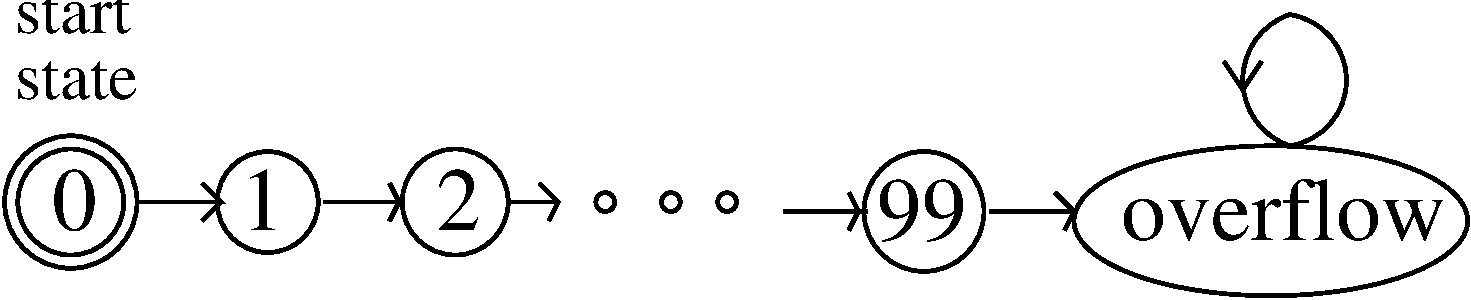
\includegraphics[height=1in]{figures/counter}
%\centerline{\psfig{figure=figures/counter.eps,height=1in}}
\caption{\em State transitions for the 99-bounded counter.}
\label{fig:counter}
\end{figure}

This machine isn't much use once it overflows, since it has no way to get
out of its overflow state.

\end{example}

\begin{example}
An unbounded counter is similar, but has an infinite state set.  This is
harder to draw \texttt{:-)}
\end{example}

\begin{example}
\textbf In the movie \textit{Die Hard 3: With a Vengeance}, the characters
played by Samuel L. Jackson and Bruce Willis have to disarm a bomb planted
by the diabolical Simon Gruber:

\textbox{
\begin{list}{}{\itemsep=0in \leftmargin=0.25in \rightmargin=0.25in}

\item[\textbf{Simon:}] On the fountain, there should be 2 jugs, do you
see them?  A 5-gallon and a 3-gallon.  Fill one of the jugs with
exactly 4 gallons of water and place it on the scale and the timer
will stop.  You must be precise; one ounce more or less will result in
detonation.  If you're still alive in 5 minutes, we'll speak.

\item[\textbf{Bruce:}] Wait, wait a second. I don't get it. Do you get it?

\item[\textbf{Samuel:}] No.

\item[\textbf{Bruce:}] Get the jugs. Obviously, we can't fill the 3-gallon jug
with 4 gallons of water.

\item[\textbf{Samuel:}] Obviously.

\item[\textbf{Bruce:}] All right. I know, here we go. We fill the 3-gallon jug
exactly to the top, right?

\item[\textbf{Samuel:}] Uh-huh.

\item[\textbf{Bruce:}] Okay, now we pour this 3 gallons into the 5-gallon jug,
giving us exactly 3 gallons in the 5-gallon jug, right?

\item[\textbf{Samuel:}] Right, then what?

\item[\textbf{Bruce:}] All right. We take the 3-gallon jug and fill it a third
of the way...

\item[\textbf{Samuel:}] No!  He said, ``Be precise.''  Exactly 4
gallons.

\item[\textbf{Bruce:}] Sh - -.  Every cop within 50 miles is running his a - - off
and I'm out here playing kids games in the park.

\item[\textbf{Samuel:}] Hey, you want to focus on the problem at hand?

\end{list}
}

Fortunately, they find a solution in the nick of time.  We'll let the
reader work out how.

The \emph{Die Hard} series is getting tired, so we propose a final
\emph{Die Hard Once and For All}.  Here Simon's brother returns to avenge
him, and he poses the same challenge, but with the 5 gallon jug replaced
by a 9 gallon one.

We can model jug-filling scenarios with a state machine.  In the scenario
with a 3 and a 5 gallon water jug, the states will be pairs, $(b,l)$ of
real numbers such that $0 \leq b \leq 5, 0 \leq l \leq 3$.  We let $b$ and
$l$ be arbitrary real numbers.  (We can prove that the values of $b$ and
$l$ will only be nonnegative integers, but we won't assume this.)  The
start state is $(0,0)$, since both jugs start empty.

Since the amount of water in the jug must be known exactly, we will only
consider moves in which a jug gets completely filled or completely
emptied.  There are several kinds of transitions:
\begin{enumerate}

\item  Fill the little jug: $(b,l) \movesto (b,3)$ for $l < 3$.

\item  Fill the big jug: $(b,l) \movesto (5,l)$ for $b<5$.

\item  Empty the little jug: $(b,l) \movesto (b,0)$ for $l>0$.

\item  Empty the big jug: $(b,l) \movesto (0,l)$ for $b>0$.

\item  Pour from the little jug into the big jug: for $l>0$,
\begin{equation*}
(b,l) \movesto
\begin{cases}
(b+l, 0) & \text{if $b + l \le 5$,}\\
(5, l - (5 - b)) & \text{otherwise.}
\end{cases}
\end{equation*}

\item Pour from big jug into little jug: for $b>0$,
\begin{equation*}
(b,l) \movesto
\begin{cases}
(0, b+l) & \text{if $b + l \le 3$,}\\
(b - (3 -l), 3) & \text{otherwise.}
\end{cases}
\end{equation*}
\end{enumerate}


Note that in contrast to the 99-counter state machine, there is more than
one possible transition out of states in the Die Hard machine.  Machines
like the 99-counter with at most one transition out of each state are
called \emph{deterministic}.  The Die Hard machine is
\emph{nondeterministic} because some states have transitions to several
different states.

\textbf{Quick exercise:} Which states of the Die Hard 3 machine have
direct transitions to exactly two states?

\end{example}

\subsection{Reachability and Preserved Invariants}

The Die Hard 3 machine models every possible way of pouring water among
the jugs according to the rules.  Die Hard properties that we want to
verify can now be expressed and proved using the state machine model.  For
example, Bruce's character will disarm the bomb if he can get to some
state of the form $(4, l)$.

A (possibly infinite) sequence of transitions through successive states
beginning at the start state corresponds to a possible system behavior;
such a sequence is called an \emph{execution} of the state machine.  A
state is called \emph{reachable} if it appears in some execution.  The
bomb in Die Hard 3 gets disarmed successfully because the state (4,3) is
reachable.

\hyperdef{invariant}{properties}{A} useful approach in analyzing state
machine is to identify properties of states that are preserved by
transitions.  

\begin{definition}
  A \term{preserved invariant} of a state machine is a predicate, $P$, on
  states, such that whenever $P(q)$ is true of a state, $q$, and $q
  \movesto r$ for some state, $r$, then $P(r)$ holds.
\end{definition}

\textbox{\begin{center}
{\Large The Invariant Principle}
\end{center}

{\large
\noindent If a preserved invariant of a state machine is true for the
start state,\\
then it is true for all reachable states.}}

The Invariant Principle is nothing more than the Induction Principle
reformulated in a convenient form for state machines.  Showing that a
predicate is true in the start state is the base case of the induction,
and showing that a predicate is a preserved invariant is the inductive
step.\footnote{Preserved invariants are commonly just called
  ``invariants'' in the literature on program correctness, but we decided
  to throw in the extra adjective to avoid confusion with other
  definitions.  For example, another subject at MIT uses ``invariant'' to
  mean ``predicate true of all reachable states.''  Let's call this
  definition ``invariant-2.''  Now invariant-2 seems like a reasonable
  definition, since unreachable states by definition don't matter, and all
  we want to show is that a desired property is invariant-2.  But this
  confuses the \emph{objective} of demonstrating that a property is
  invariant-2 with the \emph{method} for showing that it is.  After all,
  if we already knew that a property was invariant-2, we'd have no need
  for an Invariant Principle to demonstrate it.}

\subsubsection{Die Hard Once and For All}

Now back to Die Hard Once and For All.  This time there is a 9 gallon jug
instead of the 5 gallon jug.  We can model this with a state machine whose
states and transitions are specified the same way as for the Die Hard 3
machine, with all occurrences of ``5'' replaced by ``9.''

Now reaching any state of the form $(4,l)$ is impossible.  We prove this
using the Invariant Principle.  Namely, we define the preserved invariant
predicate, $P(b,l)$, to be that $b$ and $l$ are nonnegative integer
multiples of 3.  So $P$ obviously holds for the state state $(0,0)$.

To prove that $P$ is a preserved invariant, we assume $P(b,l)$ holds for
some state $(b,l)$ and show that if $(b,l) \movesto (b',l')$, then
$P(b',l')$.  The proof divides into cases, according to which transition
rule is used.  For example, suppose the transition followed from the
``fill the little jug'' rule.  This means $(b,l) \movesto (b,3)$.  But
$P(b,l)$ implies that $b$ is an integer multiple of 3, and of course 3 is
an integer multiple of 3, so $P$ still holds for the new state $(b,3)$.
Another example is when the transition rule used is ``pour from big jug
into little jug'' for the subcase that $b + l > 3$.  Then state is $(b,l)
\movesto (b -( 3 -l), 3)$.  But since $b$ and $l$ are integer multiples of
3, so is $b -( 3 -l)$.  So in this case too, $P$ holds after the
transition.

We won't bother to crank out the remaining cases, which can all be checked
just as easily.  Now by the Invariant Principle, we conclude that every
reachable state satisifies $P$.  But since no state of the form $(4,l)$
satisifies $P$, we have proved rigorously that Bruce dies once and for
all!

By the way, notice that the state (1,0), which satisfies $\QNOT(P)$, has a
transition to (0,0), which satisfies $P$.  So it's wrong to assume that
the complement of a preserved invariant is also a preserved invariant.

\subsubsection{A Robot on a Grid}

There is a robot.  It walks around on a grid, and at every step it moves
diagonally in a way that changes its position by one unit up or down
\emph{and} one unit left or right.  The robot starts at position $(0, 0)$.
Can the robot reach position $(1, 0)$?

To get some intuition, we can simulate some robot moves.  For example,
starting at (0,0) the robot could move northeast to (1,1), then southeast
to (2,0), then southwest to (1,-1), then southwest again to (0,-2).

Let's model the problem as a state machine and then find a suitable
invariant.  A state will be a pair of integers corresponding to the
coordinates of the robot's position.  State $(i,j)$ has transitions to
four different states: $(i \pm 1, j \pm 1)$.

The problem is now to choose an appropriate preserved invariant, $P$, that
is true for the start state $(0,0)$ and false for $(1, 0)$.  The Invariant
Theorem then will imply that the robot can never reach $(1, 0)$.  A direct
attempt for a preserved invariant is the predicate $P(q)$ that $q \neq (1,
0)$.

Unfortunately, this is not going to work.  Consider the state $(2,1)$.
Clearly $P(2,1)$ holds because $(2,1) \neq (1, 0)$.  And of course
$P(1,0)$ does not hold.  But $(2,1) \movesto (1,0)$, so this choice of $P$
will not yield a preserved invariant.

We need a stronger predicate.  Looking at our example execution you might
be able to guess a proper one, namely, that the sum of the coordinates is
even!  If we can prove that this is a preserved invariant, then we have
proven that the robot never reaches $(1, 0)$ ---because the sum $1+0$ of
its coordinates is odd, while the sum $0+0$ of the coordinates of the
start state is even.

\begin{theorem}
The sum of the robot's coordinates is always even.
\end{theorem}

\begin{proof}
The proof uses the Invariant Principle.

Let $P(i, j)$ be the predicate that $i + j$ is even.

First, we must show that the predicate holds for the start state $(0,0)$.
Clearly, $P(0, 0)$ is true because $0 + 0$ is even.

Next, we must show that $P$ is a preserved invariant.  That is, we must
show that for each transition $(i, j) \movesto (i', j')$, if $i + j$ is
even, then $i' + j'$ is even.  But $i' = i \pm 1$ and $j' = j \pm 1$ by
definition of the transitions.  Therefore, $i' + j'$ is equal to $i + j$
or $i + j \pm 2$, all of which are even.
\end{proof}

\begin{corollary}
The robot cannot reach $(1, 0)$.
\end{corollary}

\begin{problems}
\classproblems

\pinput{CP_robot_invariant}


\pinput{CP_98_heads_and_4_tails}

\pinput{CP_beaver_flu}

\homeworkproblems

\pinput{PS_linear_combination_game}

\pinput{PS_robot_on_2D_grid}

\pinput{PS_Zakim_bridge_state_machine}

\pinput{PS_ant_on_grid}

\pinput{PS_card_shuffle_state_machine}

\end{problems}

\textbox{
\begin{center}
{\Large Robert W. Floyd}
\end{center}

The Invariant Principle was formulated by Robert Floyd at Carnegie
Tech\footnote{The following year, Carnegie Tech was renamed
  Carnegie-Mellon Univ.} in 1967.  Floyd was already famous for work on
formal grammars which transformed the field of programming language
parsing; that was how he got to be a professor even though he never got a
Ph.D.  (He was admitted to a PhD program as a teenage prodigy, but flunked
out and never went back.)

In that same year, Albert R. Meyer was appointed Assistant Professor in
the Carnegie Tech Computer Science Department where he first met Floyd.
Floyd and Meyer were the only theoreticians in the department, and they
were both delighted to talk about their shared interests.  After just a
few conversations, Floyd's new junior colleague decided that Floyd was the
smartest person he had ever met.

Naturally, one of the first things Floyd wanted to tell Meyer about was
his new, as yet unpublished, Invariant Principle.  Floyd explained the
result to Meyer, and Meyer wondered (privately) how someone as brilliant
as Floyd could be excited by such a trivial observation.  Floyd had to
show Meyer a bunch of examples before Meyer understood Floyd's excitement
---not at the truth of the utterly obvious Invariant Principle, but rather
at the insight that such a simple theorem could be so widely and easily
applied in verifying programs.

Floyd left for Stanford the following year.  He won the Turing award
---the ``Nobel prize'' of Computer Science--- in the late 1970's, in
recognition both of his work on grammars and on the foundations of program
verification.  He remained at Stanford from 1968 until his death in
September, 2001.  You can learn more about Floyd's life and work by
reading the \href{floyd-eulogy-by-knuth.pdf}{eulogy} written by his
closest colleague, Don Knuth.

 \iffalse
   \href{http://oldwww.acm.org/pubs/membernet/stories/floyd.pdf}
{\texttt{http://oldwww.acm.org/pubs/membernet/stories/floyd.pdf}}.
\fi
}

\subsection{Sequential algorithm examples}

\subsubsection{Proving Correctness}

Robert Floyd, who pioneered modern approaches to program verification,
distinguished two aspects of state machine or process correctness:

\begin{enumerate}
\item The property that the final results, if any, of the process satisfy
system requirements.  This is called \emph{partial correctness}.

You might suppose that if a result was only partially correct, then it
might also be partially incorrect, but that's not what he meant.  The word
``partial'' comes from viewing a process that might not terminate as
computing a \emph{partial function}.  So partial correctness means that
when there is a result, it is correct, but the process might not always
produce a result, perhaps because it gets stuck in a loop.

\item The property that the process always finishes, or is guaranteed to
produce some legitimate final output.  This is called \emph{termination}.
\end{enumerate}

Partial correctness can commonly be proved using the Invariant Principle.
Termination can commonly be proved using the Well Ordering Principle.
We'll illustrate Floyd's ideas by verifying the Euclidean Greatest Common
Divisor (GCD) Algorithm.

\subsubsection{The Euclidean Algorithm}\label{euclid}

The Euclidean algorithm is a three-thousand-year-old procedure to compute
the greatest common divisor, $\gcd(a,b)$ of integers $a$ and $b$.
We can represent this algorithm as a state machine.  A state will be a
pair of integers $(x,y)$ which we can think of as integer registers in a
register program.  The state transitions are defined by the rule
\[
(x,y) \movesto (y, \remainder(x,y))
\]
for $y \neq 0$.  The algorithm terminates when no further transition is
possible, namely when $y=0$.  The final answer is in $x$.

We want to prove:
\begin{enumerate}
\item Starting from the state with $x = a$ and $y = b>0$, if we ever finish,
then we have the right answer.  That is, at termination, $x = \gcd(a,b)$.
This is a \emph{partial correctness} claim.

\item We do actually finish.  This is a process \emph{termination} claim.

\end{enumerate}

\paragraph{Partial Correctness of GCD}

First let's prove that if GCD gives an answer, it is a correct answer.
Specifically, let $d \eqdef \gcd(a,b)$.  We want to prove that \emph{if}
the procedure finishes in a state $(x,y)$, then $x = d$.

\begin{proof}
Define the state predicate
\[
P(x,y) \eqdef\ \ [\gcd(x,y) = d \text{ and } (x > 0 \text{ or } y > 0)].
\]

$P$ holds for the start state $(a,b)$, by definition of $d$ and the
requirement that $b$ is positive.  Also, the preserved invariance of
$P$ follows immediately from
\begin{lemma}\label{gcd}
For all $m,n \in \naturals$ such that $n \neq 0$,
\begin{equation}
\gcd(m,n) = \gcd(n,\remainder(m,n)).
\end{equation}
\end{lemma}

Lemma~\ref{gcd} is easy to prove: let $q$ be the quotient and $r$ be
the remainder of $m$ divided by $n$.  Then $m = qn +r$ by definition.
So any factor of both $r$ and $n$ will be a factor of $m$, and
similarly any factor of both $m$ and $n$ will be a factor of $r$.  So
$r,n$ and $m,n$ have the same common factors and therefore the same
gcd.
\iffalse and we'll leave it to the reader (a proof will appear in
later Notes on Elementary Number Theory).\fi
Now by the Invariant Principle, $P$ holds for all reachable states.

Since the only rule for termination is that $y=0$, it follows that if
$(x,y)$ is a terminal state, then $y=0$.  If this terminal state is
reachable, then the preserved invariant holds for $(x,y)$.  This implies
that $\gcd(x,0) = d$ and that $x>0$.  We conclude that $x = \gcd(x,0) =
d$.
\end{proof}

\paragraph{Termination of GCD}

Now we turn to the second property, that the procedure must terminate.  To
prove this, notice that $y$ gets strictly smaller after any one
transition.  That's because the value of $y$ after the transition is the
remainder of $x$ divided by $y$, and this remainder is smaller than $y$ by
definition.  But the value of $y$ is always a nonnegative integer, so by the
Well Ordering Principle, it reaches a minimum value among all its values
at reachable states.  But there can't be a transition from a state where
$y$ has its minimum value, because the transition would decrease $y$ still
further.  So the reachable state where $y$ has its minimum value is a
state at which no further step is possible, that is, at which the
procedure terminates.

Note that this argument does not prove that the minimum value of $y$ is
zero, only that the minimum value occurs at termination.  But we already
noted that the only rule for termination is that $y=0$, so it follows that
the minimum value of $y$ must indeed be zero.

\subsubsection{The Extended Euclidean Algorithm}\label{ExtendedGCD}

An important fact about the $\gcd(a,b)$ is that it equals an integer
linear combination of $a$ and $b$, that is,
\begin{equation}\label{sa}
\gcd(a,b) = sa+ tb
\end{equation}
for some $s,t \in \integers$.  We'll see some nice proofs
of~\eqref{sa} later when we study Number Theory, but now we'll look
at an extension of the Euclidean Algorithm that efficiently, if
obscurely, produces the desired $s$ and $t$.  It is presented here
simply as another example of application of the Invariant Method
(plus, we'll need a procedure like this when we take up number theory
based cryptography in a couple of weeks).

\emph{Don't worry if you find this Extended Euclidean Algorithm hard
  to follow, and you can't imagine where it came from.  In fact,
  that's good, because this will illustrate an important point: given
  the right prserved invariant, you can verify programs you aren't
  expected to understand.}

In particular, given nonnegative integers $x$ and $y$, with $y>0$, we
claim the following procedure\footnote{This procedure is adapted from Aho,
  Hopcroft, and Ullman's text on algorithms.}  halts with registers
\texttt{S} and \texttt{T} containing integers $s$ and $t$
satisfying~\eqref{sa}.

Inputs: $a,b \in \naturals, b>0$.

Registers: \texttt{X,Y,S,T,U,V,Q}.

Extended Euclidean Algorithm:
\begin{center}
\begin{verbatim}
X := a; Y := b; S := 0; T := 1; U := 1; V := 0; 
loop:
if Y divides X, then halt
else
  Q := quotient(X,Y);
         ;;the following assignments in braces are SIMULTANEOUS
 {X := Y,
  Y := remainder(X,Y);
  U := S,
  V := T,
  S := U - Q * S,
  T := V - Q * T};
goto loop;
\end{verbatim}
\end{center}

Note that \texttt{X,Y} behave exactly as in the Euclidean GCD algorithm in
Section~\ref{euclid}, except that this extended procedure stops one step
sooner, ensuring that $\gcd(x,y)$ is in \texttt{Y} at the end.  So for all
inputs $x,y$, this procedure terminates for the same reason as the
Euclidean algorithm: the contents, $y$, of register \texttt{Y} is a
nonnegative integer-valued variable that strictly decreases each time
around the loop.

The following properties are preserved invariants that imply partial
correctness:
\begin{eqnarray}
\gcd(X,Y) &=& \gcd(a,b), \label{XY}\\
Sa+Tb &=& Y,\text{ and }\label{SaTb}\\
Ua+Vb &=& X. \label{uaVb}
\end{eqnarray}

To verify that these are preserved invariants, note that~\eqref{XY} is the
same one we observed for the Euclidean algorithm.  To check the other two
properties, let $x,y,s,t,u,v$ be the contents of registers
\texttt{X,Y,S,T,U,V} at the start of the loop and assume that all the
properties hold for these values.  We must prove that~\eqref{SaTb}
and~\eqref{uaVb} hold (we already know~\eqref{XY} does) for the new
contents $x',y',s',t',u',v'$ of these registers at the next time the loop
is started.

Now according to the procedure, $u'=s,v'=t,x'=y$, so~\eqref{uaVb} holds
for $u',v',x'$ because of~\eqref{SaTb} for $s,t,y$.  Also, 
\[
s'= u - qs,\quad t'= v - qt,\quad y' = x - qy
\]
where $q = \quotient(x,y)$,
so
\[
s'a+t'b = (u-qs)a + (v-qt)b =ua+vb - q(sa+tb) = x - qy = y',
\]
and therefore~\eqref{SaTb} holds for $s',t',y'$.

Also, it's easy to check that all three preserved invariants are true just
before the first time around the loop.  Namely, at the start:
\begin{align*}
X      =a, Y=b,S=0, T& =1 & \mbox{so}\\
Sa+Tb = 0a+1b=b& =Y & \mbox{confirming~\eqref{SaTb}.}
\end{align*}
Also,
\begin{align*}
U     & =1, V=0, & \mbox{so} \\
Ua+Vb & = 1a+0b=a =X & \mbox{confirming~\eqref{uaVb}.  }
\end{align*}
Now by the Invariant Principle, they are true at termination.  But at
termination, the contents, $Y$, of register \texttt{Y} divides the
contents, $X$, of register \texttt{X}, so preserved invariants~\eqref{XY}
and~\eqref{SaTb} imply
\[
\gcd(a,b) = \gcd(X,Y) = Y = Sa + Tb.
\]
So we have the gcd in register \texttt{Y} and the desired coefficients in
\texttt{S}, \texttt{T}.

Now we don't claim that this verification offers much insight.  In fact,
if you're not wondering how somebody came up with this concise program and
invariant, you:
\begin{itemize}

\item are blessed with an inspired intellect allowing you to see how this
  program and its invariant were devised,

\item have lost interest in the topic, or

\item haven't read this far.

\end{itemize}
If none of the above apply to you, we can offer some reassurance by
repeating that you're not expected to understand this program.

We've already observed that a preserved invariant is really just an
induction hypothesis.  As with induction, finding the right hypothesis
is usually the hard part.
\begin{quote}
a  \textbf{Given the right preserved invariant, it can be easy to verify a
    program even if you don't understand it.}
\end{quote}
The Extended Euclidean Algorithm is an illustration of this point.

\iffalse
Once the right hypothesis or preserved
invariant is found, checking that it works is usually routine, as this
program illustrates.
\fi

\subsection{Derived Variables}

The preceding termination proofs involved finding a nonnegative
integer-valued measure to assign to states.  We might call this measure
the ``size'' of the state.  We then showed that the size of a state
decreased with every state transition.  By the Well Ordering Principle,
the size can't decrease indefinitely, so when a minimum size state is
reached, there can't be any transitions possible: the process has
terminated.

\hyperdef{derived}{vars}{More} generally, the technique of assigning
values to states ---not necessarily nonnegative integers and not necessarily
decreasing under transitions--- is often useful in the analysis of
algorithms.  \emph{Potential functions} play a similar role in physics.
In the context of computational processes, such value assignments for
states are called \emph{derived variables}.

For example, for the Die Hard machines we could have introduced a derived
variable, $f: \text{states } \to \reals$, for the amount of water in both
buckets, by setting $f((a, b)) \eqdef a + b$.  Similarly, in the robot
problem, the position of the robot along the $x$-axis would be given by
the derived variable $x\text{-coord}$, where $x\text{-coord}((i, j))
\eqdef~i$.

We can formulate our general termination method as follows:

\begin{definition}
  Let $\prec$ be a strict partial order on a set, $A$.  A derived variable
  $f : \text{states } \to A$ is \emph{strictly decreasing} iff
\[
q \movesto q' \text{  implies  } f(q') \prec f(q).
\]
\end{definition}

We confirmed termination of the GCD and Extended GCD procedures by finding
derived variables, $y$ and \texttt{Y}, respectively, that were nonnegative
integer-valued and strictly decreasing.  We can summarize this approach to
proving termination as follows:
\begin{theorem}
\label{th:decr}
If $f$ is a strictly decreasing $\naturals$-valued derived variable of a
state machine, then the length of any execution starting at state $q$ is
at most $f(q)$.
\end{theorem}

Of course we could prove Theorem~\ref{th:decr} by induction on the value
of $f(q)$, but think about what it says: ``If you start counting down at
some nonnegative integer $f(q)$, then you can't count down more than
$f(q)$ times.''  Put this way, it's obvious.

\iffalse

There are cases where it's easier to prove termination based on more
general partial orders than ``less-than'' on $\naturals$.  Termination is
guaranteed whenever there is a derived variable that strictly decreases with
respect to any well-founded partial order.

\iffalse
We now define some other useful flavors of derived variables taking values
over partial ordered sets.  We'll use the notational convention that when
$\prec$ denotes a strict partial order on some set, then $\preceq$ is the
corresponding \emph{weak} partial order
\[
a\preceq a' \ \eqdef\quad a \prec a' \lor a = a'.
\]

A relation like $\prec$ is called a \emph{strict} partial order.  It is
transitive, antisymmetric, and but \emph{non}reflexive in the strongest
sense: $a \not\prec a$ for every $a \in A$.\footnote{In other words, if $a
\prec b$, then it is not the case that $b \prec a$.  This property is also
called \emph{a}symmetry.}\fi

\begin{definition}
Let $\prec$ be a strict partial order on a set, $A$.  A derived variable
$f : Q \to A$ is \emph{strictly decreasing} with respect to $\prec$ iff
\[
q \movesto q' \text{ implies } f(q') \prec f(q).
\]
Also, $f$ is \emph{weakly decreasing} iff
\[
q \movesto q' \text{  implies  } f(q') \preceq f(q).
\]
where $\preceq$ is the weak partial order corresponding to $\prec$,
namely,
\[
[a_1 \preceq a_2] \eqdef [(a_1 \prec a_2) \text{ or } (a_1=a_2)].
\]

\emph{Strictly increasing} and \emph{weakly increasing} derived variables
are defined similarly.\footnote{Weakly increasing variables are often also
called \emph{nondecreasing}.  We will avoid this terminology to prevent
confusion between nondecreasing variables and variables with the much
weaker property of \emph{not} being a decreasing variable.}
\end{definition}

\begin{theorem}\label{well-founded-decreasing}
  If there exists a derived variable for a state machine that is strictly
  decreasing with respect to some well-founded partial order, then every
  execution terminates.
\end{theorem}

Theorem~\ref{well-founded-decreasing} follows immediately from the
\href{http://courses.csail.mit.edu/6.042/spring08/ln3.pdf#infinite.decreasing}
{observation in Notes 3} that a well-founded partial order has no infinite
decreasing sequences.

Note that the existence of a nonnegative integer-valued \emph{weakly}
decreasing derived variable does not guarantee that every execution
terminates.  That's because an infinite execution could proceed through
states in which a weakly decreasing variable remained constant.

\subsubsection{A Southeast Jumping Robot}

\iffalse Begin by defining the trivial ``pick how long'' game: P1 picks $n
\in \naturals$, the P2 and P1 alternate making forced moves.  The game
ends after $n$ forced moves; the last person to move wins.  So P1 strategy
is ``pick and even number.''  Insert here the discussion of ``terminates,
but no bound on number of steps...'' used below.

May also tell the ``guess a bigger number game''joke.
\fi

Here's a contrived but simple example of proving termination based on a
variable that is strictly decreasing over a well-founded order.  Let's
think about a robot positioned at an integer lattice-point in the
Northeast quadrant of the plane, that is, at $(x,y) \in \naturals^2$.

At every second when it is away from the origin, $(0,0)$, the robot must
make a move, which may be
\begin{itemize}

\item a unit distance West when it is not at the boundary of the Northeast
  quadrant (that is, $(x,y) \movesto (x-1,y)$ for $x>0$), or

\item a unit distance South combined with an arbitrary jump East (that is,
     $(x,y) \movesto (z,y-1)$ for $z\geq x$).

\end{itemize}
\begin{claim}\label{robotcl}
The robot will always get stuck at the origin.
\end{claim}

If we think of the robot as a nondeterministic state machine, then
Claim~\ref{robotcl} is a termination assertion.  The Claim may seem
obvious, but it really has a different character than termination based on
nonnegative integer-valued variables.  That's because, even knowing that
the robot is at position $(0,1)$, for example, there is no way to bound
the time it takes for the robot to get stuck.  It can delay getting stuck
for as many seconds as it wants by making its next move to a distant point
in the Far East.  This rules out proving termination using
Theorem~\ref{th:decr}.

So does Claim~\ref{robotcl} still seem obvious?

Well it is if you see the trick: if we reverse the coordinates, then every
robot move goes to a position that is smaller under lexicographic order.
More precisely, let $f:\naturals^2 \to \naturals^2$ be the derived variable
mapping a robot state ---its position $(x,y)$ ---to $(y,x) \in
\naturals^2$.  Now $(x,y)\movesto (x',y')$ is a legitimate robot move iff
$f((x',y')) \lex< f((x,y))$.  In particular, $f$ is a strictly
$\lex<$-decreasing derived variable, so
Theorem~\ref{well-founded-decreasing} proves that the robot always get
stuck as claimed.
\fi



\iffalse

We will prove that the robot always gets stuck at the origin by
generalizing the decreasing variable method, but with decreasing values
that are more general than nonnegative integers.  Namely, the traveling robot
can be modeled with a state machine with states of the form $((x,y),s,e)$
where
\begin{itemize}
\item $(x,y) \in \naturals^2$ is the robot's position,
\item $s$ is the number of moves South the robot took to get to this
position, and
\item $e \le 2s$ is the number of moves East the robot took to get to this
position. 
\end{itemize}

Now we define a derived variable $\vl:\text{States}\to \naturals^3$:
\[
\vl(((x,y),s,e)) \ \eqdef\quad (y,2s-e,x),
\]
and we order the values of states with the \emph{lexicographic} order,
$\lexle$, on $\naturals^3$:
\begin{equation}\label{lex3}
(k,l,m) \lexle (k',l',m') \ \eqdef\quad k < k' \text{ or } (k=k' \text{
and } l < l') \text{ or } (k=k' \text{ and } l = l' \text{ and } m \le m')
\end{equation}

Let's check that values are lexicographically decreasing.  Suppose the
robot is in state $((x,y),s,e)$.
\begin{itemize}
\item If the robot moves West it enters state $((x-1,y),s,e)$, and
\[
\vl(((x-1,y),s,e)) = (y,2s-e,x-1) \lex< (y,2s-e,x) = \vl(((x,y),s,e)),
\]
as required.


\item If the robot jumps East it enters a state $((z,y),s,e+1)$ for some
$z>x$.  Now
\[
\vl(((z,y),s,e+1)) = (y,2s-(e+1),z) = (y,2s-e-1,z),
\]
but since $2s-e-1 < 2s-e$, the rule~(\ref{lex3}) implies that
\[
\vl(((z,y),s,e+1)) = (y,2s-e-1,z)  \lex< (y,2s-e,x) = \vl(((x,y),s,e)),
\]
as required.

\item If the robot moves South it enters state $((x,y-1),s+1,e)$, and
\[
\vl(((x,y-1),s+1,e)) = (y-1,2(s+1)-e,x) \lex< (y,2s-e,x) = \vl(((x,y),s,e)),
\]
as required.

\end{itemize}

So indeed state-value is a decreasing variable under lexicographic order.
But since lexicographic order is well-founded, it is impossible for a
lexicographically-ordered value to be decreased an infinite number of
times.  That's just what we need to finish verifying Claim~\ref{robotcl}.
\fi

\begin{problems}
\homeworkproblems

\pinput{PS_divide_using_3}

\pinput{PS_filling_buckets_with_water}
\end{problems}

\hyperdef{stable}{marriage}{\section{The Stable Marriage Problem}}

Okay, frequent public reference to derived variables may not help your
mating prospects.  But they can help with the analysis!

\subsection{The Problem}

Suppose there are a bunch of boys and an equal number of girls that we
want to marry off.  Each boy has his personal preferences about the girls
---in fact, we assume he has a complete list of all the girls ranked
according to his preferences, with no ties.  Likewise, each girl has her
rank list of all of the boys.

The preferences don't have to be symmetric.  That is, Jennifer might like
Brad best, but Brad doesn't necessarily like Jennifer best.  The goal is
to marry off boys and girls: every boy must marry exactly one girl and
vice-versa ---no polygamy.  In mathematical terms, we want the mapping
from boys to their wives to be a bijection or \emph{perfect matching}.
We'll just call this a ``matching,'' for short.

Here's the difficulty: suppose \emph{every} boy likes Angelina best, and
every girl likes Brad best, but Brad and Angelina are married to other
people, say Jennifer and Billy Bob.  Now \emph{Brad and Angelina prefer
each other to their spouses}, which puts their marriages at risk: pretty
soon, they're likely to start spending late nights doing 6.042 homework
together.

This situation is illustrated in the following diagram where the digits
``1'' and ``2'' near a boy shows which of the two girls he ranks first and
which second, and similarly for the girls:

\mfigure{!}{1.2in}{figures/minWtMatch2}

More generally, in any matching, a boy and girl who are not married to
each other and who like each other better than their spouses, is called a
{\em rogue couple}.  In the situation above, Brad and Angelina would be a
rogue couple.

Having a rogue couple is not a good thing, since it threatens the
stability of the marriages.  On the other hand, if there are no rogue
couples, then for any boy and girl who are not married to each other, at
least one likes their spouse better than the other, and so won't be
tempted to start an affair.

\begin{definition}
A matching is {\em stable} iff it has no rogue couples.
\end{definition}
 
The question is, given everybody's preferences, how do you find a stable
set of marriages?  In the example consisting solely of the four people
above, we could let Brad and Angelina both have their first choices by
marrying each other.  Now neither Brad nor Angelina prefers anybody else
to their spouse, so neither will be in a rogue couple.  This leaves Jen
not-so-happily married to Billy Bob, but neither Jen nor Billy Bob can
entice somebody else to marry them.
 
It is something of a surprise that there always is a stable matching among
a group of boys and girls, but there is, and we'll shortly explain why.
The surprise springs in part from considering the apparently similar
``buddy'' matching problem.  That is, if people can be paired off as
buddies, regardless of gender, then a stable matching \emph{may not} be
possible.  For example, Figure~\ref{fig:buddy} shows a situation with a
love triangle and a fourth person who is everyone's last choice.  In this
figure Mergatoid's preferences aren't shown because they don't even
matter.   

\begin{figure}[htbp]
\centering 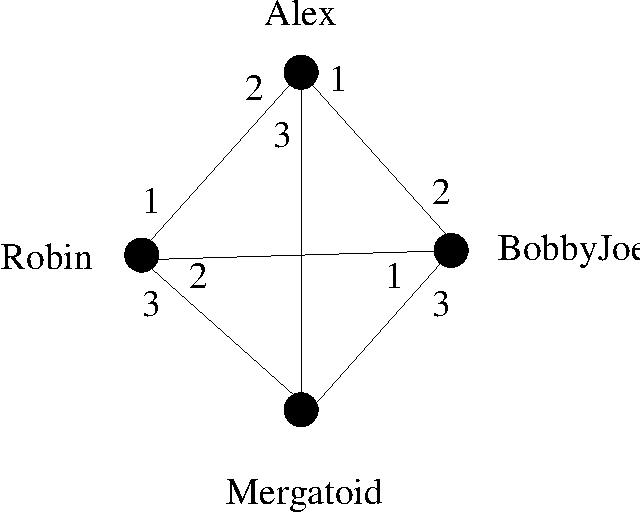
\includegraphics[height=2.3in]{figures/loveTriangle.pdf}
\caption{Some preferences with no stable buddy matching.}
\label{fig:buddy}
\end{figure}
 
Let's see why there is no stable matching: 
\begin{lemma*}
There is no stable buddy matching among the four people in
Figure~\ref{fig:buddy}.
\end{lemma*}
 
\begin{proof}
We'll prove this by contradiction.

Assume, for the purposes of contradiction, that there is a stable
matching.  Then there are two members of the love triangle that are
matched.  Since preferences in the triangle are symmetric, we may assume
in particular, that Robin and Alex are matched.  Then the other pair must
be Bobby-Joe matched with Mergatoid.

But then there is a rogue couple: Alex likes Bobby-Joe best, and Bobby-Joe
prefers Alex to his buddy Mergatoid.  That is, Alex and Bobby-Joe are a
rogue couple, contradicting the assumed stability of the matching.
\end{proof}

So getting a stable \emph{buddy} matching may not only be hard, it may be
impossible.  But when boys are only allowed to marry girls, and vice
versa, then it turns out that a stable matching is not hard to find.

%%insert rest of story from gusfield book pp3--4??

\iffalse

\subsection{Failed attempts}

Let's find a stable matching in one possible situation, and hope to
translate our method to a general algorithm.  The table below shows the
preferences of each girl and boy in decreasing order.

\begin{eqnarray*}
boys & \quad & girls \\
1 : C B E A D & \quad & A : 3 5 2 1 4 \\
2 : A B E C D & \quad & B : 5 2 1 4 3 \\
3 : D C B A E & \quad & C : 4 3 5 1 2 \\
4 : A C D B E & \quad & D : 1 2 3 4 5 \\
5 : A B D E C & \quad & E : 2 3 4 1 5
\end{eqnarray*}

How about we try a ``greedy'' strategy?\footnote{``Greedy'' is not any
moral judgment.  It refers to algorithms that work by always choosing the
next state that makes the largest immediate progress.}  We simply take
each boy in turn and pack him off with his favorite among the girls still
available.  This gives the following assignment.

\begin{eqnarray*}
1 \rightarrow C \\
2 \rightarrow A \\
3 \rightarrow D \\
4 \rightarrow B \\
5 \rightarrow E \\
\end{eqnarray*}

To determine whether this matching is stable, we have to check whether
there are any rogue couples.  Boys 1, 2, and 3 all got their top pick
among the girls; none would even think of running off.  Boy 4 may be a
problem because he likes girl $A$ better than his mate, but she ranks him
dead last.  However, boy 4 also likes girl $C$ better than his mate, and
she rates him above her own mate.  Therefore, boy 4 and girl $C$ form a
rogue couple!  The marriages are not stable.  We could try to make ad hoc
repairs, but we're really trying to develop a general strategy.

Another approach would be to use induction.  Suppose we pair Boy 1 with
his favorite girl, $C$, try to show that neither of these two will be
involved in a rogue couple, and then solve the remaining problem by
induction.  Clearly Boy 1 will never leave his top pick, Girl $C$.  But
the problem with this approach is that we \emph{can't} be sure that Girl
$C$ won't be in a rogue couple.  Girl $C$ might very well dump Boy 1 --
she might even rate him last!

This turns out to be a tricky problem.  The best approach is to use a
mating ritual that is reputed to have been popular in some mythic past.
\fi

\subsection{The Mating Ritual}

The procedure for finding a stable matching involves a \emph{Mating
Ritual} that takes place over several days.  The following events happen
each day:

{\bf Morning: } Each girl stands on her balcony.  Each boy stands under
the balcony of his favorite among the girls on his list, and he serenades
her.  If a boy has no girls left on his list, he stays home and does his
6.042 homework.

{\bf Afternoon: } Each girl who has one or more suitors serenading her,
says to her favorite suitor, ``We might get engaged.  Come back
tomorrow.''  To the others, she says, ``No.  I will never marry you!  Take
a hike!''

\textbf{Evening}: Any boy who is told by a girl to take a hike, crosses that
girl off his list.

\textbf{Termination condition}: When every girl has at most one suitor,
the ritual ends with each girl marrying her suitor, if she has one.

% Show example

There are a number of facts about this Mating Ritual that we would like to
prove:

\begin{itemize}
\item The Ritual has a last day.
\item Everybody ends up married.
\item The resulting marriages are stable.
\end{itemize}

\subsection{A State Machine Model}

Before we can prove anything, we should have clear mathematical
definitions of what we're talking about.  In this section we sketch how to
define a rigorous state machine model of the Marriage Problem.

So let's begin by formally defining the problem.

\begin{definition}
A \term{Marriage Problem} consists of two disjoint sets of the same finite
size, called \boys\ and \girls.  The members of \boys\ are called
\emph{boys}, and members of \girls\ are called \emph{girls}.  For each
boy, $B$, there is a strict total order, $<_B$, on \girls, and for each
girl, $G$, there is a strict total order, $<_G$, on \boys.  If $G_1 <_B
G_2$ we say $B$ \term{prefers} girl $G_2$ to girl $G_1$.  Similarly, if
$B_1 <_G B_2$ we say $G$ \term{prefers} boy $B_2$ to boy $B_1$.

A \emph{marriage assignment} or \term{perfect matching} is a bijection,
$w:\boys \to \girls$.  If $B \in \boys$, then $w(B)$ is called $B$'s
\emph{wife} in the assignment, and if $G \in \girls$, then $w^{-1}(G)$ is
called $G$'s \emph{husband}.  A \term{rogue couple} is a boy, $B$, and a
girl, $G$, such that $B$ prefers $G$ to his wife, and $G$ prefers $B$ to
her husband.  An assignment is \term{stable} if it has no rogue couples.
A \term{solution} to a marriage problem is a stable perfect matching.
\end{definition}

To model the Mating Ritual with a state machine, we make a key
observation: to determine what happens on any day of the Ritual, all we
need to know is which girls are on which boys' lists on the morning of
that day.  So we define a state to be some mathematical data structure
providing this information.  For example, we could define a state to be
the ``still-has-on-his-list'' relation, $R$, between boys and girls, where
$B\,R\,G$ means girl $G$ is still on boy $B$'s list.

We start the Mating Ritual with no girls crossed off.  That is, the start
state is the \emph{complete bipartite} relation in which every boy is
related to every girl.

According to the Mating Ritual, on any given morning, a boy will
\emph{serenade} the girl he most prefers among those he has not as yet
crossed out.  Mathematically, the girl he is serenading is just the
maximum among the girls on $B$'s list, ordered by $<_B$.  (If the list is
empty, he's not serenading anybody.)  A girl's \emph{favorite} is just the
maximum, under her preference ordering, among the boys serenading her.

Continuing in this way, we could mathematically specify a precise Mating
Ritual state machine, but we won't bother.  The intended behavior of the
Mating Ritual is clear enough that we don't gain much by giving a formal
state machine, so we stick to a more memorable description in terms of
boys, girls, and their preferences.  The point is, though, that it's not
hard to define everything using basic mathematical data structures like
sets, functions, and relations, if need be.

\subsection{There is a Marriage Day}

It's easy to see why the Mating Ritual has a terminal day when people
finally get married.  Every day on which the ritual hasn't terminated, at
least one boy crosses a girl off his list.  (If the ritual hasn't
terminated, there must be some girl serenaded by at least two boys, and at
least one of them will have to cross her off his list).  So starting with
$n$ boys and $n$ girls, each of the $n$ boys' lists initially has $n$
girls on it, for a total of $n^2$ list entries.  Since no girl ever gets
added to a list, the total number of entries on the lists decreases every
day that the Ritual continues, and so the Ritual can continue for at most
$n^2$ days.

\subsection{They All Live Happily Every After...}

We still have to prove that the Mating Ritual leaves everyone in a
stable marriage.  To do this, we note one very useful fact about the
Ritual: if a girl has a favorite boy suitor on some morning of the Ritual,
then that favorite suitor will still be serenading her the next morning
---because his list won't have changed.  So she is sure to have today's
favorite boy among her suitors tomorrow.  That means she will be able to
choose a favorite suitor tomorrow who is at least as desirable to her as
today's favorite.  So day by day, her favorite suitor can stay the same or
get better, never worse.  In others words, a girl's favorite is a weakly
increasing variable with respect to her preference order on the boys.

Now we can verify the Mating Ritual using a simple invariant predicate,
$P$, that captures what's going on:
\begin{quotation}
  For every girl, $G$, and every boy, $B$, if $G$ is crossed off $B$'s
  list, then $G$ has a suitor whom she prefers over $B$.
\end{quotation}

Why is $P$ invariant?  Well, we know that $G$'s favorite tomorrow will be
at least as desirable to her as her favorite today, and since her favorite
today is more desirable than $B$, tomorrow's favorite will be too.

Notice that $P$ also holds on the first day, since every girl is on every
list.  So by the Invariant Theorem, we know that $P$ holds on every day
that the Mating Ritual runs.  Knowing the invariant holds when the
Mating Ritual terminates will let us complete the proofs.

\begin{theorem}
Everyone is married by the Mating Ritual.
\end{theorem}

\begin{proof}
  Suppose, for the sake of contradiction, that it is the last day of
  the Mating Ritual and some boy does not get married.  Then he can't
  be serenading anybody, and so his list must be empty.  So by invariant
  $P$, every girl has a favorite boy whom she prefers to that boy.  In
  particular, every girl has a favorite boy whom she marries on the
  last day.  So all the girls are married.  What's more there is no
  bigamy: a boy only serenades one girl, so no two girls have the same
  favorite.

But there are the same number of girls as boys, so all the boys must be
married too.
\end{proof}

\begin{theorem}
The Mating Ritual produces a stable matching.
\end{theorem}

\begin{proof}
Let Brad be some boy and Jen be any girl that he is \emph{not} married to
on the last day of the Mating Ritual.  We claim that Brad and Jen are not
a rogue couple.  Since Brad is an arbitrary boy, it follows that no boy is
part of a rogue couple.  Hence the marriages on the last day are stable.

To prove the claim, we consider two cases:

\emph{Case} 1.  Jen is not on Brad's list.  Then by invariant $P$, we know
that Jen prefers her husband to Brad.  So she's not going to run off with
Brad: the claim holds in this case.

\emph{Case} 2.  Otherwise, Jen is on Brad's list.  But since Brad is not
married to Jen, he must be choosing to serenade his wife instead of Jen,
so he must prefer his wife.  So he's not going to run off with Jen: the
claim also holds in this case.
\end{proof}


\subsection{...Especially the Boys}

Who is favored by the Mating Ritual, the boys or the girls?  The girls
seem to have all the power: they stand on their balconies choosing the
finest among their suitors and spurning the rest.  What's more, we know
their suitors can only change for the better as the Ritual progresses.
Similarly, a boy keeps serenading the girl he most prefers among those on
his list until he must cross her off, at which point he serenades the next
most preferred girl on his list.  So from the boy's point of view, the
girl he is serenading can only change for the worse.  Sounds like a good
deal for the girls.

But it's not!  The fact is that from the beginning, the boys are
serenading their first choice girl, and the desirability of the girl being
serenaded decreases only enough to give the boy his most desirable
possible spouse.  The mating algorithm actually does as well as possible
for all the boys and does the worst possible job for the girls.

To explain all this we need some definitions.  Let's begin by observing
that while the mating algorithm produces one stable matching, there may be
other stable matchings among the same set of boys and girls.  For example,
reversing the roles of boys and girls will often yield a different stable
matching among them.

But some spouses might be out of the question in all possible stable
matchings.  For example, Brad is just not in the realm of possibility for
Jennifer, since if you ever pair them, Brad and Angelina will form a rogue
couple; here's a picture:

\mfigure{!}{1.2in}{figures/exampleOpt}

\begin{definition}
Given any marriage problem, one person is in another person's \emph{realm
of possible spouses} if there is a stable matching in which the two people
are married.  A person's {\em optimal spouse} is their most preferred
person within their realm of possibility.  A person's {\em pessimal
spouse} is their least preferred person in their realm of possibility.
\end{definition}

Everybody has an optimal and a pessimal spouse, since we know there is at
least one stable matching, namely the one produced by the Mating Ritual.
Now here is the shocking truth about the Mating Ritual:

\begin{theorem}\label{boyopt}
The Mating Ritual marries every boy to his optimal spouse.
\end{theorem}

\begin{proof}
Assume for the purpose of contradiction that some boy does not get his
optimal girl.  There must have been a day when he crossed off his optimal
girl ---otherwise he would still be serenading her or some even more
desirable girl.

By the Well Ordering Principle, there must be a \emph{first} day when a
boy, call him ``Keith,'' crosses off his optimal girl, Nicole.

According to the rules of the Ritual, Keith crosses off Nicole because
Nicole has a favorite suitor, Tom, and
\begin{quote}
Nicole prefers Tom to Keith (*)
\end{quote}
(remember, this is a proof by contradiction \texttt{:-)} ).

Now since this is the first day an optimal girl gets crossed off, we know
Tom hasn't crossed off his optimal girl.  So
\begin{quote}
Tom ranks Nicole at least as high as his optimal girl. (**)
\end{quote}
By the definition of an optimal girl, there must be some stable set of
marriages in which Keith gets his optimal girl, Nicole.  But then the
preferences given in ~(*) and~(**) imply that Nicole and Tom are a
rogue couple within this supposedly stable set of marriages (think
about it).  This is a contradiction.
\end{proof}

\begin{theorem}
The Mating Ritual marries every girl to her pessimal spouse.
\end{theorem}

\begin{proof}
Say Nicole and Keith marry each other as a result of the Mating Ritual.
By the previous Theorem~\ref{boyopt}, Nicole is Keith's optimal spouse,
and so in any stable set of marriages,
\begin{quote}
Keith rates Nicole at least as high as his spouse. (+)
\end{quote}

Now suppose for the purpose of contradiction that there is another stable
set of marriages where Nicole does worse than Keith.  That is, Nicole is
married to Tom, and
\begin{quote}
Nicole prefers Keith to Tom (++)
\end{quote}
Then in this stable set of marriages where Nicole is married to Tom,~(+)
and~(++) imply that Nicole and Keith are a rogue couple, contradicting
stability.  We conclude that Nicole cannot do worse than Keith.
\end{proof}

\begin{problems}
\practiceproblems

\pinput{TP_mating_ritual_invariant}

\homeworkproblems

\pinput{PS_stable_matching_no_first_choice}

\pinput{PS_stable_matching_non-optimal}

\pinput{PS_stable_matching_hospitals}

\pinput{PS_stable_matching_unlucky}

\end{problems}


\subsection{Applications}

Not surprisingly, a stable matching procedure is used by at least one
large dating agency.  But although ``boy-girl-marriage'' terminology is
traditional and makes some of the definitions easier to remember (we hope
without offending anyone), solutions to the Stable Marriage Problem are
widely useful.

The Mating Ritual was first announced in a paper by D. Gale and
L.S. Shapley in 1962, but ten years before the Gale-Shapley paper was
appeared, and unbeknownst to them, the Ritual was being used to assign
residents to hospitals by the National Resident Matching Program (NRMP).
The NRMP has, since the turn of the twentieth century, assigned each
year's pool of medical school graduates to hospital residencies (formerly
called ``internships'') with hospitals and graduates playing the roles of
boys and girls.  (In this case there may be multiple boys married to one
girl, but there's an easy way to use the Ritual in this situation.)
Before the Ritual was adopted, there were chronic disruptions and awkward
countermeasures taken to preserve assignments of graduates to residencies.
The Ritual resolved these problems so successfully, that it was used
essentially without change at least through 1989.\footnote{Much more about
the Stable Marriage Problem can be found in the very readable mathematical
monograph by Dan Gusfield and Robert W. Irving,
\href{http://mitpress.mit.edu/catalog/item/default.asp?ttype=2&tid=7676}{The
Stable Marriage Problem: Structure and Algorithms}, MIT Press, Cambridge,
Massachusetts, 1989, 240 pp.}

MIT Math Prof.\ Tom Leighton, who regularly teaches 6.042 and also founded
the internet infrastructure company, Akamai, reports another application.
Akamai uses a variation of the Gale-Shapley procedure to assign web
traffic to servers.  In the early days, Akamai used other combinatorial
optimization algorithms that got to be too slow as the number of servers
and traffic increased.  Akamai switched to Gale-Shapley since it is fast
and can be run in a distributed manner.  In this case, the web traffic
corresponds to the boys and the web servers to the girls.  The servers
have preferences based on latency and packet loss; the traffic has
preferences based on the cost of bandwidth.

\endinput
 %invariants, termination via well-founded posets,
                         %stable marriage *Albert

\hyperdef{recursive}{data}{\chapter{Recursive Data Types}}
%\coursecopyright

\emph{Recursive data types} play a central role in programming.  From a
Mathematical point of view, recursive data types are what induction is
about.  Recursive data types are specified by \emph{recursive definitions}
that say how to build something from its parts.  These definitions have
two parts:
\begin{itemize}
\item \textbf{Base case(s)} that don't depend on anything else.
\item \textbf{Constructor case(s)} that depend on previous cases.
\end{itemize}

\hyperdef{paren}{string}{\section{Strings of Parentheses}}

Let $\prns$ be the set of all strings of parentheses.  For example,
the following two strings are in $\prns$:
\begin{equation}\label{2strings}
\mtt{())((((())}\quad \text{and}\quad \mtt{((())())()}
\end{equation}
Since we're just starting to study recursive data, just for practice we'll
formulate $\prns$ as a recursive data type,

\begin{definition}\label{prns-def}
The data type, $\prns$, of strings of parentheses is defined recursively:

\begin{itemize}

\item \textbf{Base case:} The \term{empty string}, $\emptystring$, is in
  $\prns$.

\item \textbf{Constructor case:} If $s \in \prns$, then
$s\mtt{)}$ and $s\mtt{(}$ are in $\prns$.

\end{itemize}

\end{definition}

Here we're writing $s\mtt{)}$ to indicate the string that is sequence of
parentheses (if any) in the string $s$, followed by a right parenthesis;
similarly for $s\mtt{(}$.

A string, $s \in \prns$, a called a \term{matched string} if its
parentheses ``match up'' in the usual way.  For example, the left hand
string above is not matched because its second right parenthesis does not
have a matching left parenthesis.  The string on the right is matched.

One precise way to determine if a string is matched is to start with 0 and
read the string from left to right, adding 1 to the count for each left
parenthesis and subtracting 1 from the count for each right parenthesis.
For example, here are the counts for the two strings above
\[\begin{array}{rrrrrrrrrrrrr}
& \mtt{(} & \mtt{)} & \mtt{)} & \mtt{(} & \mtt{(} & \mtt{(} & \mtt{(} &
\mtt{(} & \mtt{)} & \mtt{)} & \mtt{)} & \mtt{)}\\
0 & 1 & 0 & -1 & 0 & 1 & 2 & 3 & 4 & 3 & 2 & 1 & 0\\
\\
\\
& \mtt{(} & \mtt{(} & \mtt{(} & \mtt{)} & \mtt{)} & \mtt{(} & \mtt{)} &
\mtt{)} & \mtt{(} & \mtt{)}\\
0 & 1 & 2 & 3 & 2 & 1 & 2 & 1 & 0 & 1 & 0
\end{array}\]
A string has a \term{good count} if its running count never goes
negative and ends with 0.  So the second string above has a good count, but
the first one does not because its count went negative at the third step.
\begin{definition}\label{gc-def}
Let
\[
\GC \eqdef \set{ s \in \prns \suchthat s\ \text{has a good count}}.
\]
\end{definition}
The matched strings can now be characterized precisely as this set of
strings with good counts.  But it turns out to be really useful to
characterize the matched strings in another way as well, namely, as a
recursive data type:

\begin{definition}\label{RM-def}
Recursively define the set, $\RM$, of strings as follows:
\begin{itemize}

\item \textbf{Base case:} $\emptystring \in\RM$.

\item \textbf{Constructor case:} If $s,t \in\RM$, then
\[
\mtt{(}s\mtt{)}t \in\RM.
\]

\end{itemize}

\end{definition}


Here we're writing $\mtt{(}s\mtt{)}t$ to indicate the string that
starts with a left parenthesis, followed by the sequence of parentheses
(if any) in the string $s$, followed by a right parenthesis, and ending
with the sequence of parentheses in the string $t$.

Using this definition, we can see that $\emptystring \in\RM$ by the Base
case, so
\[
\mtt{(}\emptystring\mtt{)}\emptystring=\mtt{()}\in\RM
\]
by the Constructor case.  So now,
\begin{align*}
\mtt{(}\emptystring\mtt{)}\mtt{()} &= \mtt{()()} \in \RM
    & \text{(letting $s = \emptystring, t = \mtt{()}$)}\\
\mtt{(())}\emptystring & = \mtt{(())} \in \RM
    & \text{(letting $s = \mtt{()}, t = \emptystring$)}\\
&\ \ \mtt{(())()} \in \RM
    & \text{(letting $s = \mtt{()}, t = \mtt{()}$)}
\end{align*}
are also strings in $\RM$ by repeated applications of the Constructor
case.

\textbf{Quickie:} Verify that $\mtt{((())())()} \in \RM$.

It may not be obvious, but $\RM = \GC$.  We'll confirm this later.

\section{Arithmetic Expressions}
Expression evaluation is a key feature of programming languages, and
recognition of expressions as a recursive data type is a key to
understanding how they can be processed.

To illustrate this approach we'll work with a toy example: arithmetic
expressions like $3x^2 + 2x + 1$ involving only one variable, ``$x$.''
We'll refer to the data type of such expressions as $\aexp$.  Here is its
definition:

\begin{definition}\label{A}
The set, $\aexp$, of \emph{Arithmetic expressions} in the variable, $x$,
is defined recursively as follows:

\begin{itemize}
\item \textbf{Base cases:}

\begin{enumerate}

\item The variable, $x$, is in $\aexp$.

\item The arabic numeral, $\mtt{k}$, for any nonnegative integer, $k$, is
  in $\aexp$.

\end{enumerate}

\item \textbf{Constructor cases:} If $e,f \in \aexp$, then
\begin{enumerate}
\setcounter{enumi}{2}

\item $(e \sumsym f) \in \aexp$.  The expression $(e \sumsym f)$ is called a
  \term{sum}.  The \aexp's $e$ and $f$ are called the \term{components} of
  the sum; they're also called the \term{summands}.

\item $(e \prodsym f) \in \aexp$.  The expression $(e \prodsym f)$ is called a
  \term{product}.  The \aexp's $e$ and $f$ are called the
  \term{components} of the product; they're also called the
  \term{multiplier} and \term{multiplicand}.

\item $\minussym(e) \in \aexp$.  The expression $\minussym(e)$ is called a
  \term{negative}.
\end{enumerate}
\end{itemize}
\end{definition}

Notice that \aexp's are fully parenthesized, and exponents aren't allowed.
So the $\aexp$ version of the polynomial expression $3x^2 + 2x + 1$ would
officially be written as
\begin{equation}\label{fullparens}
((\mtt{3} \prodsym (x \prodsym x)) \sumsym ((\mtt{2} \prodsym x) \sumsym \mtt{1})).
\end{equation}
These parentheses and $\ast$'s clutter up examples, so we'll often use
simpler expressions like ``$3x^2 + 2x + 1$'' instead
of~\eqref{fullparens}.  But it's important to recognize that $3x^2 + 2x +
1$ is not an \aexp; it's an \emph{abbreviation} for an $\aexp$.

\iffalse

 being represented as
a tagged datum.  To start, we might represent 0 as a length one sequence
consisting of the tag \texttt{zero}:
\begin{definition}
The nonnegative integers can be defined recursively as follows:

\begin{definition}\label{tagn}
\begin{itemize}
\item \textbf{Base case}  $\ang{\texttt{zero}}\in \naturals$.
\item \textbf{Constructor case} if $n \in \naturals$, then
      $\ang{\texttt{successor},n}\in \naturals$.
\end{itemize}

\end{definition}
\fi


\iffalse
\begin{example}
The set, $\List$, of \emph{pure lists} is defined recursively by:
\begin{enumerate}
\item The 0-tuple, $\nillist$, is in $\List$.
\item If $\ell_1$ and $\ell_2$ are in $\List$, then the pair $(\ell_1,
\ell_2)$ is in $\List$.
\end{enumerate}

In Lisp-like programming languages, the pairing operation is called
\texttt{cons} and the 0-tuple is called \texttt{nil}.

\end{example}
\fi


%% Structural Induction on Recursive Data Types %%%%%%%%%%%%%%%%%%%%%%%%%%%%%%%
\section{Structural Induction on Recursive Data Types}

\hyperdef{struct}{induction}{Structural} induction is a method for proving
some property, $P$, of all the elements of a recursively-defined data
type.  The proof consists of two steps:
\begin{itemize}
\item Prove $P$ for the base cases of the definition. 
\item Prove $P$ for the constructor cases of the definition, assuming that it
  is true for the component data items.  
\end{itemize}

A very simple application of structural induction proves that the
recursively defined matched strings always have an equal number of left
and right parentheses.  To do this, define a predicate, $P$, on strings $s
\in \prns$:
\[
P(s) \eqdef\ \ s \text{ has an equal number of left and right parentheses}.
\]
\begin{proof}

  We'll prove that $P(s)$ holds for all $s \in\RM$ by structural induction
  on the definition that $s \in\RM$, using $P(s)$ as the induction
  hypothesis.

\textbf{Base case:} $P(\emptystring)$ holds because the empty string has zero
left and zero right parentheses.

\textbf{Constructor case:} For $r = \mtt{(}s\mtt{)}t$, we must show
that $P(r)$ holds, given that $P(s)$ and $P(t)$ holds.  So let $n_s$,
$n_t$ be, respectively, the number of left parentheses in $s$ and $t$.  So
the number of left parentheses in $r$ is $1+n_s+n_t$.

Now from the respective hypotheses $P(s)$ and $P(t)$, we know that the
number of right parentheses in $s$ is $n_s$, and likewise, the number of
right parentheses in $t$ is $n_t$.  So the number of right parentheses in
$r$ is $1+n_s+n_t$, which is the same as the number of left parentheses.
This proves $P(r)$.  We conclude by structural induction that $P(s)$ holds
for all $s \in\RM$.
\end{proof}

\begin{notesproblem}
\bparts
\ppart Give an easy proof using structural induction that every recursively
defined match string has a good count.  That is
\[
\RM \subseteq \GC.
\]
\ppart Conversely, prove by induction on the length of strings that the
every string with a good count has a recursive definition, that is,
\[
\GC \subseteq \RM.
\]

\eparts
\end{notesproblem}

\subsection{Functions on Recursively-defined Data Types}

Functions on recursively-defined data types can be defined recursively
using the same cases as the data type definition.  Namely, to define a
function, $f$, on a recursive data type, define the value of $f$ for the
base cases of the data type definition, and then define the value of $f$
in each constructor case in terms of the values of $f$ on the component
data items.

\iffalse

For example, some basic functions on strings have simple recursive
definitions based on a recursive definition of strings as a tagged datum:

\begin{definition}\label{A*}
The set, $A^*$, of strings over a set, $A$, called the \emph{alphabet},
is defined recursively as follows:
\begin{itemize}
\item \textbf{Base case:} $\ang{\texttt{emptystring}} \in A^*$.

\item \textbf{Constructor case:} if $s \in A^*$ and $a \in A$, then
$\ang{\texttt{successor-string},s,a}\in A^*$.

\end{itemize}
\end{definition}
Here, of course, $\ang{\texttt{emptystring}}$ is a tagged representation
of the emptystring, $\emptystring$, and
\[
\ang{\texttt{successor-string}, s, a}
\]
is a tagged representation of the string, $sa$, equal to the string $s$,
followed by the character, $a$.

Now we give a recursive definition of the \emph{length} of a string.
\begin{definition}
The \emph{length}, $\lnth{s}$, of a string, $s$, is defined recursively by
the rules:
\begin{itemize}
\item $\lnth{\emptystring} \eqdef 0$
\item $\lnth{sa} \eqdef 1+\lnth{s}$.
\end{itemize}
\end{definition}

\begin{definition}
The \emph{concatenation}, $st$, of strings $s$ and $t$ over an alphabet,
$A$, is defined recursively on $t$ by the rules:
\begin{itemize}
\item $s\emptystring \eqdef s$.
\item $s(ta) \eqdef (st)a$ for $a \in A$.
\end{itemize}
\end{definition}
\fi

For example, from the recursive definition of the set, $\RM$, of strings of
matched parentheses, we define:
\begin{definition}
The \emph{depth}, $d(s)$, of a string, $s \in\RM$, is defined
recursively by the rules:
\begin{itemize}
\item $d(\emptystring) \eqdef 0.$
\item $d(\mtt{(}s\mtt{)}t)
    \eqdef \max \set{d(s) + 1, d(t)}$
\end{itemize}
\end{definition}

\textbox{\textbf{Warning:} When a recursive definition of a data type
allows the same element to be constructed in more than one way, the
definition is said to be \emph{ambiguous}.  A function defined recursively
from an ambiguous definition of a data type will not be well-defined
unless the values specified for the different ways of constructing the
element agree.}

We were careful to choose an \emph{un}ambiguous definition of $\RM$ to
ensure that functions defined recursively on the definition would always
be well-defined.  As an example of the trouble an ambiguous definition can
cause, let's consider yet another definition of the matched strings.

\iffalse Recursive definitions of tagged data types, where the tag
uniquely determines the rule used to construct an element, are guaranteed
to be unambiguous.
\fi

\begin{example}\label{M}
  Define the set, $M \subseteq \prns$ recursively as follows:
\begin{itemize}

\item \textbf{Base case:} $\emptystring \in M$,

\item \textbf{Constructor cases:} if $s,t \in M$, then
the strings $\mtt{(}s\mtt{)}$ and $st$ are also in $M$.
\end{itemize}
\end{example}

\begin{notesproblem}
Give an easy proof by structural induction that $M =\RM$.
\end{notesproblem}

Since $M = \RM$, and the definition of $M$ seems more straightforward, why
didn't we use it?  Because the definition of $M$ is ambiguous, while the
trickier definition of $\RM$ is unambiguous.  Does this ambiguity matter?
Yes it does.  For suppose we defined
\begin{align*}
  f(\emptystring)        & \eqdef 1,\\
  f(\ \mtt{(}s\mtt{)}\ ) & \eqdef 1+ f(s),\\
  f(st)                  & \eqdef (f(s)+1) \cdot (f(t)+1)
                            & \text{for } st\neq \emptystring.
\end{align*}

Let $a$ be the string $\mtt{(())} \in M$ built by two successive
applications of the first $M$ constructor starting with $\emptystring$.  Next
let $b \eqdef aa$ and $c \eqdef bb$, each built by successive applications
of the second $M$ constructor starting with $a$.

Alternatively, we can build $ba$ from the second constructor with $s=b$
and $t=a$, and then get to $c$ using the second constructor with $s=ba$
and $t=a$.

Now by these rules, $f(a) = 2$, and $f(b) = (2+1)(2+1)=9$.  This means
that $f(c) = f(bb)= (9+1)(9+1)=100$.

But also $f(ba) = (9+1)(2+1) = 27$, so that $f(c) = f(ba\,a) = (27 +1)
(2+1) = 84$.

The outcome is that $f(c)$ is defined to be both 100 and 84, which shows
that the rules defining $f$ are inconsistent.

On the other hand, structural induction remains a sound proof method even
for ambiguous recursive definitions, which is why it was easy to prove
that $M=\RM$.

\subsection{Recursive Functions on Nonnegative Integers}

The nonnegative integers can be understood as a recursive data type.
\begin{definition}\label{0succ}
The set, $\naturals$, is a data type defined recursivly as:
\begin{itemize}
\item $0 \in \naturals$.
\item If $n \in \naturals$, then the \emph{successor}, $n+1$, of $n$ is in
$\naturals$.
\end{itemize}

\end{definition}

This of course makes it clear that ordinary induction is simply the
special case of structural induction on the recursive
Definition~\ref{0succ}, This also justifies the familiar recursive
definitions of functions on the nonnegative integers.  Here are some
examples.

\begin{description}
\item[The Factorial function.] This function is often written ``$n!$.''
You will see a lot of it later in the term.  Here we'll use the notation
$\text{fac}(n)$:
\begin{itemize}
\item $\text{fac}(0) \eqdef 1$.
\item $\text{fac}(n+1) \eqdef (n+1)\cdot \text{fac}(n)$ for $n \ge 0$.
\end{itemize}

\item[The Fibonacci numbers.]  Fibonacci numbers arose out of an effort 800
  years ago to model population growth.  They have a continuing fan club of
  people captivated by their extraordinary properties.  The $n$th Fibonacci
  number, $\text{fib}$, can be defined recursively by:
\begin{align*}
\text{fib}(0) &\eqdef 0,\\ 
\text{fib}(1) &\eqdef 1,\\ 
\text{fib}(n) &\eqdef \text{fib}(n-1) + \text{fib}(n-2) &\mbox{for $n \geq 2$.} 
\end{align*}
Here the recursive step starts at $n=2$ with base cases for 0 and 1.  This
is needed since the recursion relies on two previous values.

\iffalse
What is $\text{fib}(4)$?  Well, $\text{fib}(2) =
\text{fib}(1)+\text{fib}(0) = 1$, $\text{fib}(3) =
\text{fib}(2)+\text{fib}(1) = 2$, so $\text{fib}(4) = 3$.  The sequence
starts out $0, 1, 1, 2, 3, 5, 8, 13, 21,\dots$.
\fi

\item[Sum-notation.]  Let ``$S(n)$'' abbreviate the expression
``$\sum_{i=1}^n f(i)$.''  We can recursively define $S(n)$ with the rules
  \begin{itemize}
  \item $S(0) \eqdef 0$.
  \item $S(n+1) \eqdef  f(n+1) + S(n)$ for $n\geq 0$.
  \end{itemize}

\iffalse
\item[Simultaneous recursive definitions:]
  You can define several things at the same time, in terms of each
  other.  For example, we may define two functions $f$ and $g$ from
  $\naturals$ to $\naturals$, recursively, by:
  \begin{itemize}
  \item
    $f(0) \eqdef 1$,
  \item
    $g(0) \eqdef 1$,
  \item
    $f(n+1) \eqdef f(n) + g(n)$, for $n \geq 0$,
  \item
    $g(n+1) \eqdef f(n) \times g(n)$, for $n \geq 0$.
  \end{itemize}
\fi

\end{description}

\iffalse

\begin{optional}

We can use the recursive definition of a function to establish its
properties by structural induction.

As an illustration, we'll prove a cute identity involving Fibonacci
numbers.  Fibonacci numbers provide lots of fun for mathematicians because
they satisfy many such identities.
\begin{proposition}
  $\forall n \geq 0 (\Sigma_{i=0}^n F_i^2 = F_n F_{n+1})$.
\end{proposition}

Example: $n = 4$:
\[
0^2 + 1^2 + 1^2 + 2^2 + 3^2 = 15 = 3 \cdot 5.
\]
Let's try a proof by (standard, not strong) induction.  The theorem
statement suggests trying it with $P(n)$ defined as:
\[
\sum_{i=0}^n F_i^2 = F_n F_{n+1}.
\]

\textbf{Base case} ($n=0$). 
$\Sigma_{i=0}^0 F_i^2 \eqdef (F_0)^2 = 0 = F_0 F_1$ because
$F_0 \eqdef 0$.

\textbf{Inductive step} ($n\geq 0$).  Now we stare at the gap between
$P(n)$ and $P(n+1)$.  $P(n+1)$ is given by a summation that's obtained
from that for $P(n)$ by adding one term; this suggests that, once again,
we subtract.  The difference is just the term $F_{n+1}^2$.  Now, we are
assuming that the original $P(n)$ summation totals $F_n F_{n+1}$ and want
to show that the new $P(n+1)$ summation totals $F_{n+1} F_{n+2}$.  So we
would {\em like\/} the difference to be
\[
F_{n+1} F_{n+2} - F_n F_{n+1}.
\]

So, the actual difference is $F_{n+1}^2$ and the difference we want is
$F_{n+1} F_{n+2} - F_n F_{n+1}$.  Are these the same?  We want to check
that:
\[
F_{n+1}^2 = F_{n+1} F_{n+2} - F_n F_{n+1}.
\]
But this is true, because it is really the Fibonacci definition in
disguise: to see this, divide by $F_{n+1}$.

\end{optional}
\fi

\subsubsection{Ill-formed Function Definitions}

There are some \hyperdef{ill}{formed}{blunders} to watch out for when
defining functions recursively.  Below are some function specifications
that resemble good definitions of functions on the nonnegative integers,
but they aren't.

\begin{eqnarray}\label{f1}
f_1(n)\eqdef 2+f_1(n-1).
\end{eqnarray}
This ``definition'' has no base case.  If some function, $f_1$,
satisfied~(\ref{f1}), so would a function obtained by adding a constant to
the value of $f_1$.  So equation~(\ref{f1}) does not uniquely define
an $f_1$.

\begin{eqnarray}\label{f2}
f_2(n) \eqdef
\begin{cases}
 0, & \text{if $n=0$},\\
 f_2(n+1) &  \text{otherwise}.
\end{cases}
\end{eqnarray}
This ``definition'' has a base case, but still doesn't uniquely determine
$f_2$.  Any function that is 0 at 0 and constant everywhere else would
satisfy the specification, so~\eqref{f2} also does not uniquely define
anything.

In a typical programming language, evaluation of $f_2(1)$ would begin with
a recursive call of $f_2(2)$, which would lead to a recursive call of
$f_2(3)$, \dots with recursive calls continuing without end.  This
``operational'' approach interprets~\eqref{f2} as defining a
\emph{partial} function, $f_2$, that is undefined everywhere but 0.

\begin{eqnarray}\label{f3}
f_3(n) \eqdef \begin{cases}
  0, &  \text{if $n$ is divisible by 2,}\\
  1, &  \text{if $n$ is divisible by 3,}\\
  2, & \text{otherwise.}
 \end{cases}
\end{eqnarray}
This ``definition'' is inconsistent: it requires $f_3(6) = 0$ and $f_3(6)
=1$, so~(\ref{f3}) doesn't define anything.

\subsubsection{A Mysterious Function}
Mathematicians have been wondering about this function specification for a
while:
\begin{eqnarray}\label{f5}
f_4(n) \eqdef\begin{cases}
 1, & \text{if $n\le 1$},\\
 f_4(n/2) &  \text{if $n>1$ is even},\\
 f_4(3n+1)& \text{if $n>1$ is odd}.
\end{cases}
\end{eqnarray}
For example, $f_4(3)=1$ because
\[
f_4(3)\eqdef f_4(10)\eqdef f_4(5)\eqdef f_4(16)\eqdef f_4(8)\eqdef
f_4(4)\eqdef f_4(2)\eqdef f_4(1)\eqdef 1.
\]
The constant function equal to 1 will satisfy~\eqref{f5}, but it's not
known if another function does too.  The problem is that the third case
specifies $f_4(n)$ in terms of $f_4$ at arguments larger than $n$, and so
cannot be justified by induction on $\naturals$.  It's known that any
$f_4$ satisfying~\eqref{f5} equals 1 for all $n$ up to over a billion.

\textbf{Quick exercise:} Why does the constant function 1
satisfy~\eqref{f5}?

\iffalse

\section{Tagged data}

Labelling a recursively defined data item with a tag that uniquely
determines the rule used to construct it is a standard approach to avoiding
unambiguous recursive definitions in programming.

For example, arithmetic expressions like
\begin{equation}\label{ax}
-(a(x\cdot x)+ bx) + 1
\end{equation}
are another important example of a recursive data type.  We could define
them as parenthesized strings with symbols for arithmetic operators and
names for variables and constants, but a tagged representation is more
useful:

\begin{definition}\label{A}
The set, $\aexp$, of \emph{Arithmetic expressions} over a set of
\emph{variables}, $V$, is defined recursively as follows:
\begin{itemize}
\item \textbf{Base cases:}
\begin{enumerate}
\item If $n \in \integers$, then $\ang{\texttt{int}, n} \in \aexp$.
\item If $v \in V$, then $\ang{\texttt{var}, v} \in \aexp$.
\end{enumerate}
\item \textbf{Constructor cases:} if $e,e' \in \aexp$, then
\begin{enumerate}
\item $\ang{\texttt{sum}, e, e'} \in \aexp$,
\item $\ang{\texttt{prod}, e, e'} \in \aexp$, and
\item $\ang{\texttt{minus}, e} \in \aexp$.
\end{enumerate}
\end{itemize}
\end{definition}

So the $\aexp$ corresponding to formula~\ref{ax} would be:
\begin{equation}\label{axtag}
\begin{array}{rll}
\left< \right. \texttt{sum}, 
         & \left< \right. \texttt{minus},\ \ \left< \right. \texttt{sum},
               & \ang{\texttt{prod},\ \ \ang{\texttt{var},\ a},
                                     \ang{\texttt{prod},\ \
                                            \ang{\texttt{var},\ x},\
                                            \ang{\texttt{var},\ x}}},\\
                               && \left. \left. \ang{\texttt{prod},\ \
                                       \ang{\texttt{var},\ b},\
                                       \ang{\texttt{var},\ x}}
                                   \right> \right>,\\
         & \left. \left. \ang{\texttt{int},\ 1} \right> \right>
\end{array}
\end{equation}
Now the expression~\ref{ax} is certainly a lot more humanly intelligible
than~\ref{axtag}, but is in fact the preferred representation in
programming.

the parse tree of Figure~\ref{fig:parse} is

uses the \emph{parse trees} of the expressions,
rather than strings.  Figure~\ref{fig:parse} shows a
parse tree for expression~\eqref{ax}.

\begin{figure}[htbp]
\centering 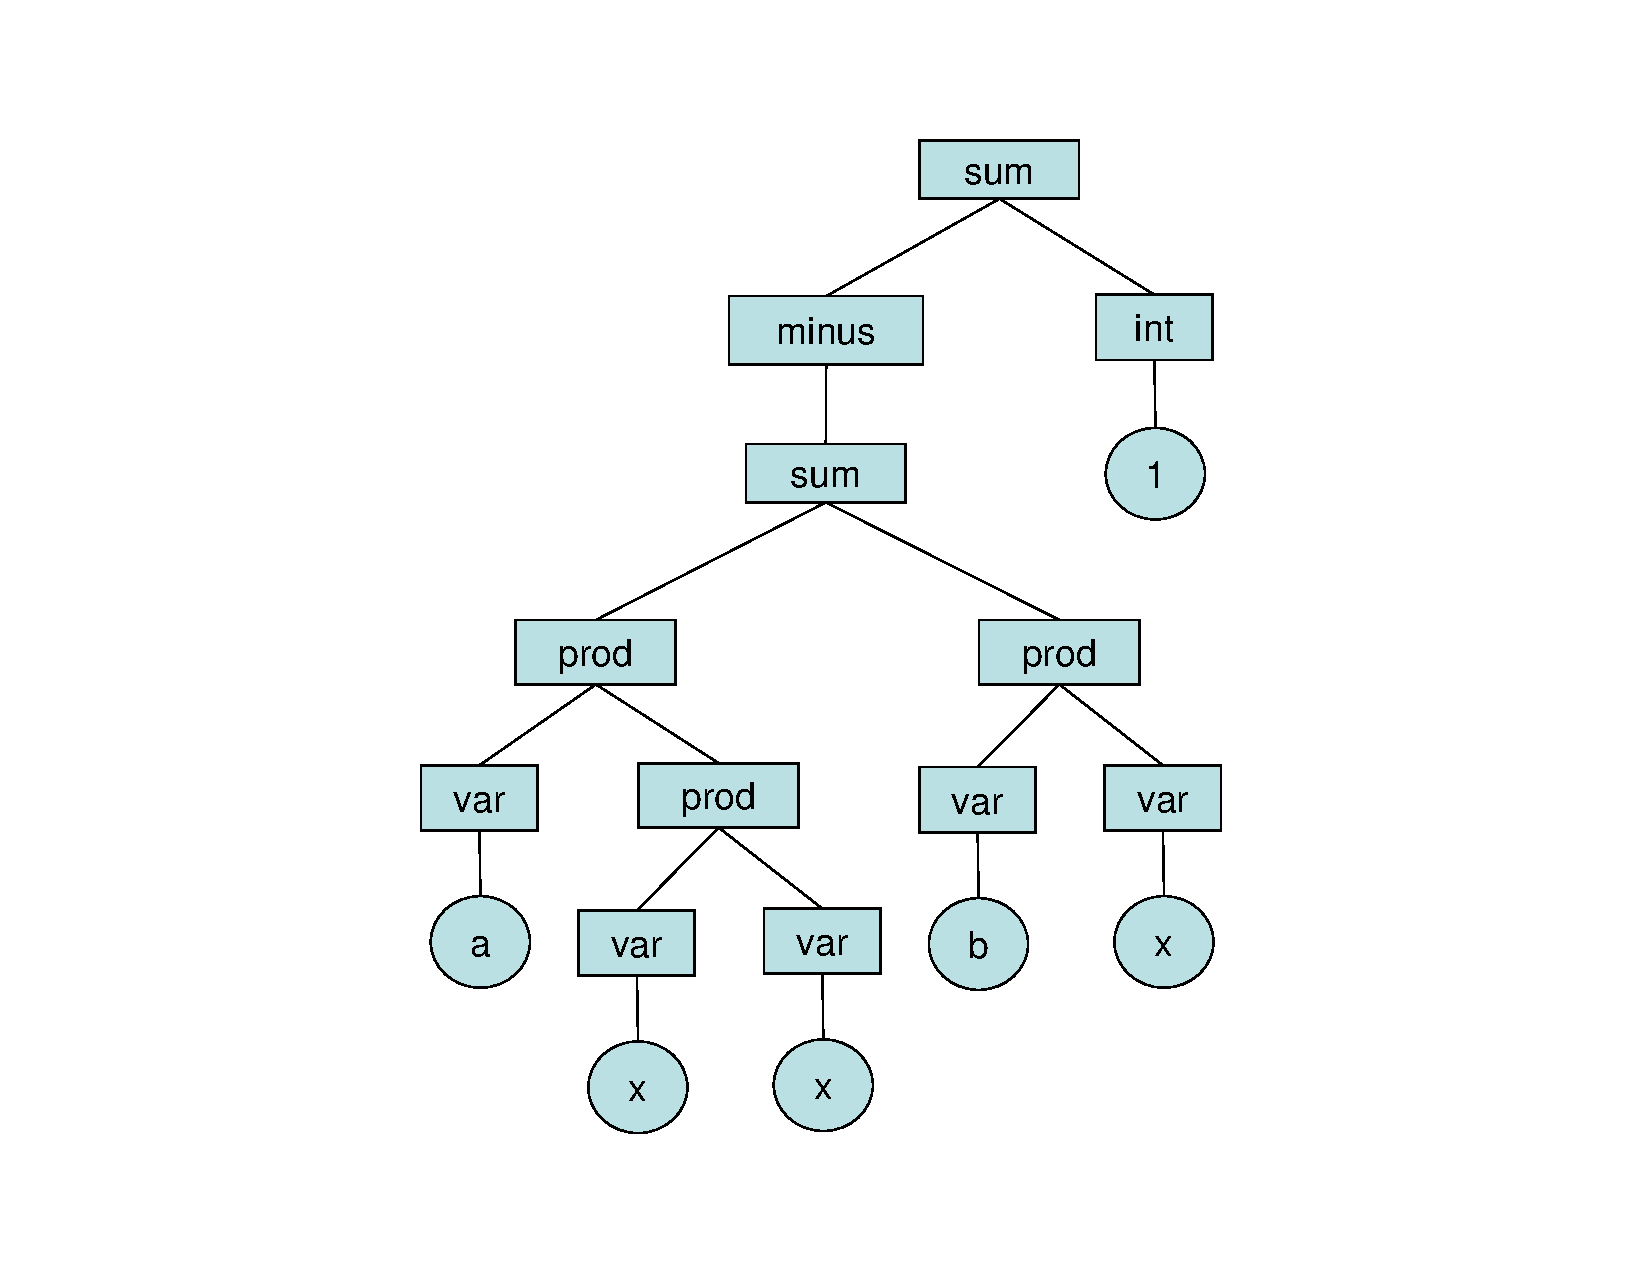
\includegraphics[height=4.5in]{figures/parsetree.pdf}
\caption{Parse tree for $-(a(x\cdot x)+ bx) + 1$.}
\label{fig:parse}
\end{figure}


Such a tree would be represented by pairs or triples that begin with a
\emph{tag} equal to the label of the top node of the parse tree.  We'll
call these tagged data items $\aexp$'s.  
\fi


\subsection{Evaluation and Substitution with Aexp's}

\subsubsection{Evaluating Aexp's}

Since the only variable in an \aexp\ is $x$, the value of an \aexp\ is
determined by the value of $x$.  For example, if the value of $x$ is 3,
then the value of $3x^2 + 2x + 1$ is obviously 34.  In general, given any
$\aexp$, $e$, and an integer value, $n$, for the variable, $x$, we can
evaluate $e$ to finds its value, $\meval(e,n)$.  It's easy, and useful, to
specify this evaluation process with a recursive definition.

\begin{definition}\label{meval-def}
  The \term{evaluation function}, $\meval: \aexp \times \integers \to
  \integers$, is defined recursively on expressions, $e \in \aexp$, as
  follows.  Let $n$ be any integer.

\begin{itemize}
\item \textbf{Base cases:}

\begin{enumerate}

\item\label{eval-var} Case[$e$ is $x$]
\[
\meval(x, n) \eqdef n.
\]
(The value of the variable, $x$, is given to be $n$.)

\item\label{eval-const} Case[$e$ is $\mtt{k}$]
\[
\meval(\mtt{k}, n) \eqdef k.
\]
(The value of the numeral $\mtt{k}$ is the integer $k$, no matter what
value $x$ has.)

\end{enumerate}

\item \textbf{Constructor cases:}

\begin{enumerate}
\setcounter{enumi}{2}

\item\label{eval-sum} Case[$e$ is $(e_1 \sumsym e_2)$]
\[
\meval((e_1 \sumsym e_2),n) \eqdef
  \meval(e_1,n)+\meval(e_2,n).
\]

\item\label{eval-prod} Case[$e$ is $(e_1 \prodsym e_2)$]
\[
\meval((e_1 \prodsym e_2),n) \eqdef \meval(e_1,n) \cdot \meval(e_2,n).
\]

\item\label{eval-minus} Case[$e$ is $\minussym(e_1)$]
\[
\meval(\minussym(e_1),n) \eqdef - \meval(e_1,n).
\]
\end{enumerate}

\end{itemize}

\end{definition}

For example, here's how the recursive definition of $\meval$ would arrive at
the value of $3+x^2$ when $x$ is 2:
\begin{align*}
\meval((\mtt{3} \sumsym (x \prodsym x)),2)
 & = \meval(\mtt{3},2) + \meval((x \prodsym x),2)
                  & \text{(by~Def~\ref{meval-def}.\ref{eval-sum})}\\
 & = 3 + \meval((x \prodsym x),2) & \text{(by~Def~\ref{meval-def}.\ref{eval-const})}\\
 & = 3 + (\meval(x,2) \cdot \meval(x,2)) & \text{(by~Def~\ref{meval-def}.\ref{eval-prod})}\\
 & = 3 + (2 \cdot 2) & \text{(by~Def~\ref{meval-def}.\ref{eval-var})}\\
 & = 3 + 4 = 7.
\end{align*}

\subsubsection{Substituting into Aexp's}
Substituting expressions for variables is a standard, important
operation.  For example the result of substituting the expression $3x$ for $x$
in the $(x(x-1))$ would be $(3x(3x-1)$.  We'll use the general
notation $\msubst{f}{e}$ for the the result of substituting an $\aexp$, $f$,
for each of the $x$'s in an $\aexp$, $e$.  For instance,
\[
\msubst{3x}{x(x-1)} = 3x(3x-1).
\]

This substitution function has a simple recursive definition:

\begin{definition}\label{subst-def}
  The \term{substitution function} from $\aexp \times \aexp$ to \aexp\ is
  defined recursively on expressions, $e \in \aexp$, as follows.  Let $f$
  be any $\aexp$.

\begin{itemize}
\item \textbf{Base cases:}

\begin{enumerate}

\item\label{subst-var} Case[$e$ is $x$]
\[
\msubst{f}{x} \eqdef f.
\]
(The result of substituting $f$ for the variable, $x$, is just $f$.)

\item\label{subst-const} Case[$e$ is $\mtt{k}$]
\[
\msubst{f}{\mtt{k}} \eqdef \mtt{k}.
\]
(The numeral, $\mtt{k}$, has no $x$'s in it to substitute for.)

\end{enumerate}

\item \textbf{Constructor cases:}

\begin{enumerate}
\setcounter{enumi}{2}
\item\label{subst-sum} Case[$e$ is $(e_1 \sumsym e_2)$]
\[
\msubst{f}{(e_1 \sumsym e_2)}) \eqdef  (\msubst{f}{e_1} \sumsym
\msubst{f}{e_2}).
\]

\item\label{subst-prod} Case[$e$ is $(e_1 \prodsym e_2)$]
\[
\msubst{f}{(e_1 \prodsym e_2)}) \eqdef  (\msubst{f}{e_1} \prodsym
\msubst{f}{e_2}).
\]

\item\label{subst-minus} Case[$e$ is $\minussym(e_1)$]
\[
\msubst{f}{\minussym(e_1)} \eqdef \minussym (\msubst{f}{e_1}).
\]

\end{enumerate}
\end{itemize}
\end{definition}

Here's how the recursive definition of the substitution function would find
the result of substituting $3x$ for $x$ in the $x(x-1)$:
\begin{align*}
\msubst{3x}{(x(x-1))} & =
\msubst{3x}{(x \prodsym (x \sumsym \minussym(1)))} & \text{(unabbreviating)}\\
 & = (\msubst{3x}{x} \prodsym \msubst{3x}{(x \sumsym \minussym(1))})
         & \text{(by~Def~\ref{subst-def}~\ref{subst-prod})}\\
 & = (3x \prodsym \msubst{3x}{(x \sumsym \minussym(1))})
         & \text{(by~Def~\ref{subst-def}~\ref{subst-var})}\\
 & = (3x \prodsym (\msubst{3x}{x} \sumsym \msubst{3x}{\minussym(1)}))
         & \text{(by~Def~\ref{subst-def}~\ref{subst-sum})}\\
 & = (3x \prodsym (3x \sumsym \minussym (\msubst{3x}{1})))
         & \text{(by~Def~\ref{subst-def}~\ref{subst-var} \&~\ref{subst-minus})}\\
 & = (3x \prodsym (3x \sumsym \minussym (1)))
         & \text{(by~Def~\ref{subst-def}~\ref{subst-const})}\\
 & = 3x(3x-1) & \text{(abbreviation)}
\end{align*}

Now suppose we have to find the value of $\msubst{3x}{(x(x-1))}$ when $x =
2$.  There are two approaches.

First, we could actually do the substitution above to get $3x(3x-1)$, and
then we could evaluate $3x(3x-1)$ when $x =2$, that is, we could
recursively calculate $\meval(3x(3x-1),2)$ to get the final value 30.  In
programming jargon, this would be called evaluation using the
\emph{Substitution Model}.  Tracing through the steps in the evaluation,
we find that the Substitution Model requires two substitutions for
occurrences of $x$ and 5 integer operations: 3 integer multiplications, 1
integer addition, and 1 integer negative operation.  Note that in this
Substitution Model the multiplication $3 \cdot 2$ was performed twice to
get the value of 6 for each of the two occurrences of $3x$.

The other approach is called evaluation using the \emph{Environment
  Model}.  Namely, we evaluate $3x$ when $x = 2$ using just 1
multiplication to get the value 6.  Then we evaluate $x(x-1)$ when $x$ has
this value 6 to arrive at the value $6\cdot 5=30$.  So the Environment
Model requires 2 variable lookups and only 4 integer operations: 1
multiplication to find the value of $3x$, another multiplication to find
the value $6 \cdot 5$, along with 1 integer addition and 1 integer
negative operation.

So the Environment Model approach of calculating
\[
\meval(x(x-1), \meval(3x,2))
\]
instead of the Substitution Model approach of calculating
\[
\meval(\msubst{3x}{x(x-1)},2)
\]
is faster.  But how do we know that these final values reached by these
two approaches always agree?  We can prove this easily by structural
induction on the definitions of the two approaches.  More precisely, what
we want to prove is

\begin{theorem}\label{environments}
For all expressions $e,f \in \aexp$ and $n \in \integers$,
\begin{equation}\label{eval-subst}
\meval(\msubst{f}{e},n) = \meval(e, \meval(f,n)).
\end{equation}
\end{theorem}

\begin{proof}
The proof is by structural induction on $e$.\footnote{This is an example
of why it's useful to notify the reader what the induction variable is
---in this case it isn't $n$.}

\textbf{Base cases:}
\begin{itemize}

\item Case[$e$ is $x$]

  The left hand side of equation~\eqref{eval-subst} equals $\meval(f,n)$
  by this base case in Definition~\ref{subst-def} of the substitution
  function, and the right hand side also equals $\meval(f,n)$ by this base
  case in Definition~\ref{meval-def} of $\meval$.


\item Case[$e$ is $\mtt{k}$].

  The left hand side of equation~\eqref{eval-subst} equals $\mtt{k}$ by
  this base case in Definitions~\ref{subst-def} and~\ref{meval-def} of
  the substitution and evaluation functions.  Likewise, the right hand
  side equals $\mtt{k}$ by two applications of this base case in the
  Definition~\ref{meval-def} of $\meval$.

\end{itemize}

\textbf{Constructor cases}:
\begin{itemize}

\item Case[$e$ is $(e_1 \sumsym e_2)$]

  By the structural induction hypothesis~\eqref{eval-subst}, we may assume
  that for all $f \in \aexp$ and $n \in \integers$,

\begin{equation}\label{ln4.hyp}
\meval(\msubst{f}{e_i},n)  =  \meval(e_i, \meval(f,n))
\end{equation}
for $i= 1,2$.  We wish to prove that

\begin{equation}\label{s+}
\meval(\msubst{f}{(e_1\sumsym e_2)},n)  =  \meval((e_1 \sumsym e_2), \meval(f,n))
\end{equation}

But the left hand side of~(\ref{s+}) equals
\[
\meval(\, (\msubst{f}{e_1} \sumsym \msubst{f}{e_2}),\ n)
\]
by Definition~\ref{subst-def}.\ref{subst-sum} of substitution into a sum
expression.  But this equals
\[
\meval(\msubst{f}{e_1},n) + \meval(\msubst{f}{e_2},n)
\]
by Definition~\ref{meval-def}.\ref{eval-sum} of $\meval$ for a sum expression.  By
induction hypothesis~\eqref{ln4.hyp}, this in turn equals
\[
\meval(e_1,\meval(f,n)) + \meval(e_2,\meval(f,n)).
\]
Finally, this last expression equals the right hand side of~(\ref{s+}) by
Definition~\ref{meval-def}.\ref{eval-sum} of $\meval$ for a sum
expression.  This proves~(\ref{s+}) in this case.

\item $e$ is $(e_1 \prodsym e_2)$.  Similar.

\item $e$ is $-(e_1)$.  Even easier.

\end{itemize}

This covers all the constructor cases, and so completes the proof by
structural induction.

\end{proof}


\iffalse
\subsection{A String Theorem}

Here is a more complex proof, illustrating a combination of structural
induction and strengthening the hypothesis.

\begin{theorem}
  In a string of $0$s and $1$s, the number of occurrences of the pattern
  $01$ is less than or equal to the number of occurrences of $10$, plus
  one.
\end{theorem}

Let's try to prove this by structural induction.  First we must
define $P(s)$.  Let's write $\ms{num}(pat,s)$ as the number of
occurrences of the pattern string pat in s.  Now our inductive
hypothesis is
\[
P(s): \ms{num}(01,s) \leq \ms{num}(10,s) + 1. 
\]
If you try to prove this by structural induction, you will get
stuck.
Why? 
Consider what happens when you add $1$ at the end.  
This could increase the number of $01$s without increasing the number of
$10$s. 

So, to prove by structural induction on strings, let's strengthen the
hypothesis by adding another clause.  If a string ends in $0$ then
the number of $01$s is less than or equal to the number of $10$s.
That solves the problem by weakening what we have to show when the
string ends in $1$.  But maybe it causes another problem somewhere
else.  Let's give it a try:

Redefine $P(s) \eqdef$
\begin{eqnarray*}
\ms{num}(01,s) & \leq & \ms{num}(10,s) + 1, \text{ and}\\
\leftenq{\text{If $s$ ends in $0$ then}}\\
\ms{num}(01,s) & \leq  &\ms{num}(10,s).
\end{eqnarray*} 
 
This means that, for each inductive step have two things to show.

\structuredproof{

  Prove: $\forall s \in S \; (P(s))$ \\
  1. (Base) $P(\emptystring)$ 
  \reason{No patterns of either kind.} \\
  2. (Inductive step) $\forall s \in S \; (P(s) \implies P(s 0))$ \\
  1. Fix $s$. \\
  2. Assume $P(s)$. \\
  3. $P(s 0)$ \\
  1. $\ms{num}(01,s0) \leq \ms{num}(10,s0) + 1$. 
  \reason{???} \\
  2. If $s 0$ ends in $0$ then $\ms{num}(01,s0) \leq
  \ms{num}(10,s0)$. \noreason \\
  \reason{???} \\
  3. QED
  \reason{Conjunction} \\
  4. QED 
  \reason{Implication, UG} \\
  3. (Inductive step) $\forall s \in S \; (P(s) \implies P(s 1))$ \\
  1. Fix $s$. \\
  2. Assume $P(s)$. \\
  3. $P(s 1)$ \\
  1. $\ms{num}(01,s1) \leq \ms{num}(10,s1) + 1$. 
  \reason{???} \\
  2. If $s 1$ ends in $0$ then $\ms{num}(01,s1) \leq
  \ms{num}(10,s1)$.\noreason \\
  \reason{???} \\
  3. QED
  \reason{Conjunction} \\
  4. QED 
  \reason{Implication, UG} \\
  4. QED
  \reason{Structural induction on strings.}\\
}

First let's consider $s1$. This is the case that looks dangerous,
because it might increase the number of $01$s.  We have to prove two
statements.  The second is easy, because the new string doesn't end in
$0$.  We say it's ``vacuously true''.

The first statement now takes some work. 
We might be adding to the number of $01$s.  
However, if we do, the previous string must have ended with $0$. 
Then the inductive hypothesis says that the previous string had to
satisfy the stronger inequality in the second statement. 
Adding one to the LHS of the stronger inequality yields the weaker
inequality we want.

The following proof fragment considers cases based on whether $s$ ends
in $0$ or not.  If not, it might end in $1$, or might be empty (don't
forget this possibility).

\begin{proof}
  3. $P(s 1)$ \\
  1. $\ms{num}(01,s1) \leq \ms{num}(10,s1) + 1$. \\
  1. If $s$ ends in $0$ then $\ms{num}(01,s1) \leq\ms{num}(10,s1) + 1$. \\
  1. Assume $s$ ends in $0$. \\
  2. $\ms{num}(01,s) \leq \ms{num}(10,s)$ 
  Inductive hypothesis (3.2), part 2. \\
  3. $\ms{num}(01,s1) = \ms{num}(01,s) + 1$ 
  Adding one more $01$. \\
  4. $\ms{num}(10,s1) = \ms{num}(10,s)$ \\
  5. $\ms{num}(01,s1) \leq\ms{num}(10,s1) + 1$. 
  Algebra (combining 3.3.1.1.2, ...3, and ...4) \\
  QED 
  Implication \\
  2. If $s$ ends in $1$ then $\ms{num}(01,s1)\leq\ms{num}(10,s1) + 1$. \\
  Inductive hypothesis, part 1; no new $01$s. \\
  3. If $s = \emptystring$ then $\ms{num}(01,s1) \leq\ms{num}(10,s1)+ 1$. \\
  $s1$ is just $1$, which has no $01$s. \\
  4. QED 
  Cases \\
  2. If $s 1$ ends in $0$ then $\ms{num}(01,s1) \leq \ms{num}(10,s1)$. \\
  Vacuously true, because $s1$ doesn't end in $0$. \\
  3. QED
  Conjunction \\
\end{proof}
Of course, you could also expand the step for $s$ ending in $1$ into a
careful series of inequalities.

Now consider $s0$.  We hope that what we did to make the $s1$ case
work doesn't mess up the $s0$ case.  But we have to check.

The first statement is easy.  It follows from the first statement of
the inductive hypothesis for $s$, because we are not increasing the
number of $01$s.  But now the second statement takes more work.  The
difficulty is that the new string ends in $0$, which means that we
have to show the stronger inequality in the second statement.  But to
do this, we might only have the weaker inequality for the previous
string.  The argument again depends on what the previous string $s$
ended with.  So again, we consider cases, based on whether $s$ ends in
$0$ or $1$, or is empty.  If $s$ ends in $0$ we rely on the second
statement of the inductive hypothesis for $s$ (with the stronger
inequality), whereas if $s$ ends in $1$ we rely on the first statement
(with the weaker inequality).  In this case, we have to ``turn the
weaker inequality into the stronger inequality''.

\structuredproof[38ex]{
  3. $P(s 0)$ \\
  1. $\ms{num}(01,s0) \leq \ms{num}(10,s0) + 1$.
  \reason{Induct. hypothesis, part 1; no new $01$s.} \\
  2. If $s 0$ ends in $0$ then $\ms{num}(01,s0) \leq\ms{num}(10,s0)$. \\
  1. $\ms{num}(01,s0) \leq \ms{num}(10,s0)$. \\
  1. If $s$ ends in $0$ then $\ms{num}(01,s0)
  \leq\ms{num}(10,s0)$. \noreason \\
  \reason{Induct. hypothesis, part 2; no new $01$s} \\
  2. If $s$ ends in $1$ then $\ms{num}(01,s0)
  \leq\ms{num}(10,s0)$. \noreason \\ 
  1. Assume $s$ ends in $1$. \\
  2. $\ms{num}(01,s) \leq \ms{num}(10,s) + 1$. 
  \reason{Inductive hypothesis, part 1} \\
  3. $\ms{num}(01,s0) = \ms{num}(01,s)$ \\
  4. $\ms{num}(10,s0) = \ms{num}(10,s) + 1$ 
  \reason{Exactly one new occurrence of $10$.} \\
  5. $\ms{num}(01,s0) \leq \ms{num}(10,s0)$ 
  \reason{Algebra} \\
  6. QED
  \reason{Implication} \\
  3. If $s = \emptystring$ then $\ms{num}(01,s0) \leq
  \ms{num}(10,s0)$. \noreason \\ 
  
\reason{$s0$ is just $1$, which has no $01$s or $10$s.} \\
  4. QED 
  \reason{Cases} \\
  2. QED
  \reason{Propositional reasoning (truth table)} \\
  3. QED 
  \reason{Conjunction}\\
}

If you actually write out all these cases in the proof, you will
notice that some facts are stated repeatedly, e.g., that when you add
a $0$ to the end of a string you are not increasing the number of
$01$s.  To avoid having to state these facts several times, you can
move them earlier in the proof.
\fi


\iffalse

\begin{example*}
\begin{definition}\label{E}
Define a set, $E$, recursively as follows:
\begin{itemize}
\item \textbf{Base case:} $0 \in E$,\label{0E}
\item \textbf{Constructor cases:} if $n \in E$, then
\begin{enumerate}
\item $n+2 \in E$, when $n\geq 0$;\label{+2E}
\item $-n \in E$, when $n > 0$.\label{-E}
\end{enumerate}
\end{itemize}

\end{definition}
\end{example*}

Using this definition, we can see that $0 \in E$ by the Base case, so $0 +
2 = 2 \in E$ by Constructor case~\ref{+2E}., and so $2+2 =4 \in E$, $4+2 =
6 \in E$, \dots, and in fact any nonnegative even number is in $E$ by
successive application of case~\ref{+2E}.  Also, by case~\ref{-E}.,
$-2,-4,-6,\dots \in E$.  So clearly all the even integers are in $E$.

Is anything else in $E$?  The definition doesn't say so explicitly, but an
implicit condition on a recursive definition is that the only way things
get into $E$ is as a consequence of the Base and Constructor cases.  In
other words, $E$ will be exactly the set of even integers.

A very simple application of structural induction proves that the set $E$
given by Definition~\ref{E} is exactly the set of even numbers.  We already
explained why all the even numbers are in $E$.  So what's left is to show
that:

\begin{lemma*}
Every number in the set $E$ in Definition~\ref{E} is even.
\begin{proof}
The proof is by structural induction on $n \in E$.  The induction
hypothesis is 
\[
Q(n) \eqdef \text{$n$ is even}.
\]

\textbf{Base case}: $Q(0)$ holds since 0 is even.

\textbf{Constructor cases}: assuming $n \in E$ and $Q(n)$ holds, prove
that
\begin{itemize}

\item $Q(n+2)$ holds.  This is immediate, since adding 2 to an even number
  gives an even number.

\item $Q(-n)$ holds.  This is also immediate, since $n$ is even iff $-n$ is
even.

\end{itemize}

This completes the proof of the Constructor cases, and we conclude by
structural induction at $Q(n)$ holds for all $n \in E$.
\end{proof}

\end{lemma*}


defining the set, $E$, of even numbers as in Definitions~\ref{E}, but
without the conditions~\ref{+2E}.\ and~\ref{-E}.\ that restrict application of
the rules.  Namely,

\begin{definition}\label{Eamb}
Define a set, $E'$, recursively as follows:
\begin{itemize}
\item \textbf{Base case:} $0 \in E'$,\label{0Eamb}
\item \textbf{Constructor cases:} if $n \in E'$, then
\begin{enumerate}
\item $n+2 \in E'$, \label{+2Eamb}
\item $-n \in E'$.\label{-Eamb}
\end{enumerate}
\end{itemize}
\end{definition}

Now Definition~\ref{Eamb} is perfectly legitimate, and we could us it to
prove by structural induction that $E'$ also is the set of even integers,
that is, $E'= E$.  But Definition~\ref{Eamb} is ambiguous.  For example,
$0\in E'$ by the base case, but also $0=-0 \in E'$ by applying constructor
case~\ref{-Eamb} to the base case.  This begins to matter when we try to
define a function, $s$, from $E'$ to nonnegative integers based on
Definition~\ref{Eamb}:
\begin{align*}
  s(0) & \eqdef 1,\\
s(n+2) & \eqdef 1+ s(n),\\
 s(-n) & \eqdef 1+ s(n).
\end{align*}
So $s(0) \eqdef 1$ by the base case of this definition, and also $s(0)=
s(-0) \eqdef 1+s(0) = 1 + 1 = 2$ by the second constructor case, which
shows that these rules are inconsistent.

On the other hand, using the unambiguous Definition~\ref{E} of $E$,
essentially the same definition of $S$ works just fine.  Namely, define
\begin{align*}
  s(0) & \eqdef 1,\\
  s(n+2) & \eqdef 1+ s(n), & \text{ for } n \geq 0\\
  s(-n) & \eqdef 1+ s(n) & \text{ for } n > 0.
\end{align*}
Now $s(n)$ is unambiguously defined, and in fact is precisely the (unique)
number of steps required to construct $n \in E$ according to the
unambiguous Definition~\ref{E} of $E$.
\fi

%% Structural Induction on Recursive Data Types Problems %%%%%%%%%%%%%%%%%%%%%%
%\startclassproblems
\pinput{CP_F18_functions}
\pinput{CP_recursively_defined_sets}
\pinput{CP_erasable_strings}
\pinput{CP_binary_trees}


%% Games as a Recursive Data Type %%%%%%%%%%%%%%%%%%%%%%%%%%%%%%%%%%%%%%%%%%%%%
\section{Games as a Recursive Data Type}

Chess, Checkers, and Tic-Tac-Toe are examples of \emph{two-person
terminating games of perfect information}, ---$\tg$'s for short.  These
are games in which two players alternate moves that depend only on the
visible board position or state of the game.  ``Perfect information''
means that the players know the complete state of the game at each move.
(Most card games are \emph{not} games of perfect information because
neither player can see the other's hand.)  ``Terminating'' means that play
cannot go on forever ---it must end after a finite number of
moves.\footnote{Since board positions can repeat in chess and checkers,
termination is enforced by rules that prevent any position from being
repeated more than a fixed number of times.  So the ``state'' of these
games is the board position \emph{plus} a record of how many times
positions have been reached.}

We will define $\tg$'s \iffalse in a straightforward way tagged\fi as a 
recursive data type.  To see how this will work, let's use the game of
Tic-Tac-Toe as an example.

\subsection{Tic-Tac-Toe}

Tic-Tac-Toe is a game for young children.  There are two players who
alternately write the letters ``X'' and ``O'' in the empty boxes of a $3
\times 3$ grid.  Three copies of the same letter filling a row, column, or
diagonal of the grid is called a \emph{tic-tac-toe}, and the first player
who gets a tic-tac-toe of their letter wins the game.  \iffalse Children
generally don't take long to figure out an optimal strategy for playing the
game.\fi


We're now going give a precise mathematical definition of the Tic-Tac-Toe
\term{game tree} as a recursive data type.  \iffalse and carefully defining
the allowed moves Children of course have no need for such a definition,
and it would be too complicated for them anyway.  But if we had to write a
Tic-Tac-Toe playing \emph{computer program}, we'd need this kind of picky
precision.\fi Here's the idea behind the definition: at any point in the
game, the ``board position'' is the pattern of X's and O's on the $3 \times
3$ grid.  From any such Tic-Tac-Toe pattern, there are a number of next
patterns that might result from a move.  For example, from the initial
empty grid, there are nine possible next patterns, each with a single X in
some grid cell and the other eight cells empty.  From any of these
patterns, there are eight possible next patterns gotten by placing an O in
an empty cell.  These move possibilities are given by the
\hyperdef{game}{tree}{game tree} for Tic-Tac-Toe indicated in
Figure~\ref{fig:Tic-Tac-Toe}.

\begin{figure}[htbp]
\centering
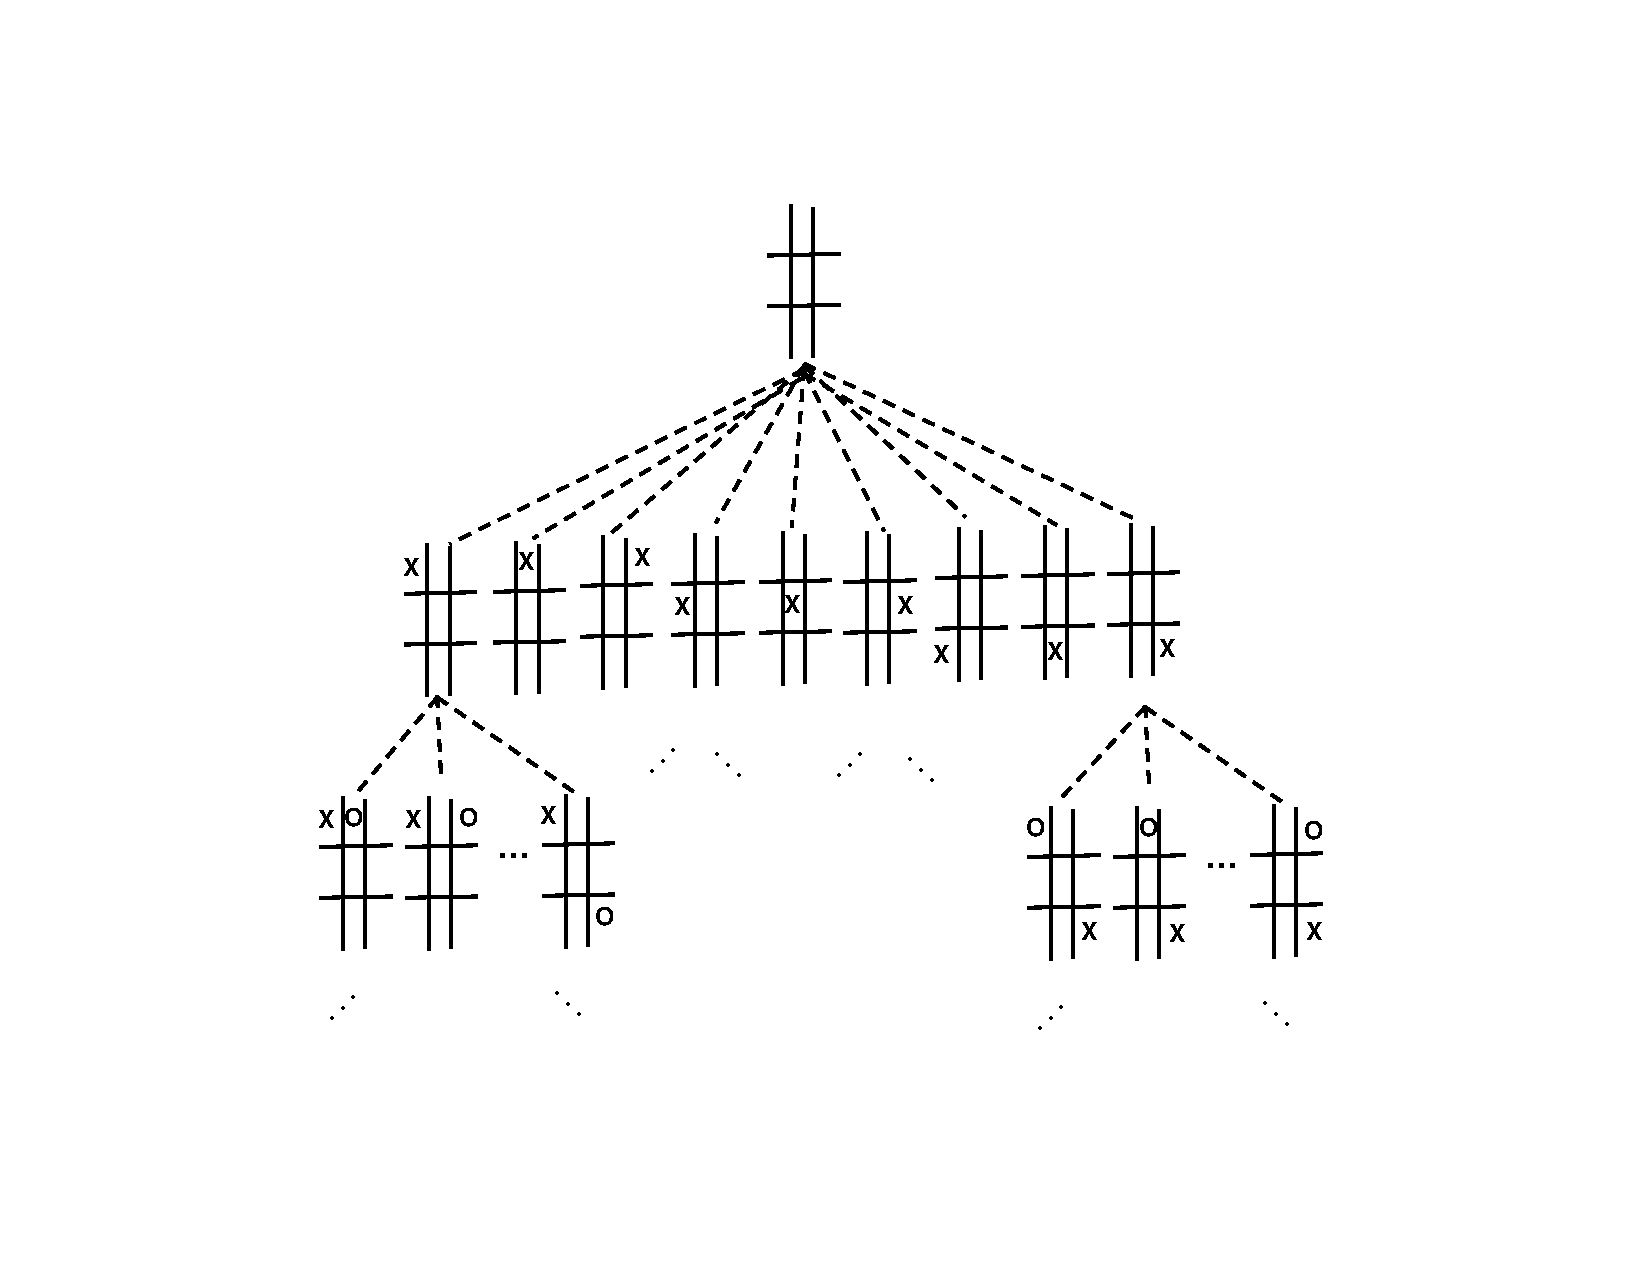
\includegraphics[height=6in]{figures/topgame.pdf}
\caption{The Top of the Game Tree for Tic-Tac-Toe.}
\label{fig:Tic-Tac-Toe}
\end{figure}


\iffalse
\[\begin{array}{c|c|c}
\hspace{.1in} & \hspace{.1in} & \hspace{.1in}\\
\hline  & &\\
\hline  & &
\end{array}\]

\textbf{FIGURE NEEDED}
\fi

\begin{definition}

A Tic-Tac-Toe \emph{pattern} is a $3 \times 3$ grid each of whose 9 cells
contains either the single letter, X, the single letter, O, or is
empty.
\iffalse
Moreover, there must be either
\begin{itemize}

\item one more X than O's, with at most two tic-tac-toes of X's, and no
tic-tac-toe of O's, or

\item an equal number of X's and O's, with at most one tic-tac-toes of
O's, and no tic-tac-toe of X's.
\end{itemize}
\fi

A pattern, $Q$, is a \emph{possible next pattern after} $P$, providing $P$
has no tic-tac-toes and
\begin{itemize}

\item if $P$ has an equal number of X's and O's, and $Q$ is the same as
$P$ except that a cell that was empty in $P$ has an X in $Q$, or

\item if $P$ has one more X than O's, and $Q$ is the same as $P$ except
that a cell that was empty in $P$ has an O in $Q$.
\end{itemize}

If $P$ is a Tic-Tac-Toe pattern, and $P$ has no next patterns, then the
\emph{terminated Tic-Tac-Toe game trees} at $P$ are

\begin{itemize}

\item 
\[
\ang{P, \ang{\texttt{win}}},
\]
if $P$ has a tic-tac-toe of X's.


\item 
\[
\ang{P, \ang{\texttt{lose}}},
\]
if $P$ has a tic-tac-toe of O's.


\item
\[
\ang{P, \ang{\texttt{tie}}},
\]
otherwise.

\end{itemize}


\iffalse
If $Q$ is a possible move from $P$, then the game tree starting at $Q$ is
called a \emph{  Notice
that $\mathcal{G}_P = \emptyset$ iff $P$ is terminated.}
\fi

The \emph{Tic-Tac-Toe game trees starting at $P$} are defined recursively:

\textbf{Base Case}:
A terminated Tic-Tac-Toe game tree at $P$ is a Tic-Tac-Toe game tree
starting at $P$.

\textbf{Constructor case}: If $P$ is a non-terminated Tic-Tac-Toe pattern,
then the Tic-Tac-Toe game tree starting at $P$ consists of $P$ and the set
of all game trees starting at possible next patterns after $P$.
\end{definition}

For example, if
\begin{align*}
P_0 & =  \begin{array}{c|c|c}
                O & X & O\\
         \hline X & O & X\\
         \hline X & &
        \end{array}\\
Q_1 & = \begin{array}{c|c|c}
                O & X & O\\
         \hline X & O & X\\
         \hline X &  & O
        \end{array}\\
Q_2 & = \begin{array}{c|c|c}
                O & X & O\\
         \hline X & O & X\\
         \hline X & O & 
        \end{array}\\
R & = \begin{array}{c|c|c}
                O & X & O\\
         \hline X & O & X\\
         \hline X & O & X
        \end{array}
\end{align*}
the game tree starting at $P_0$ is pictured in Figure~\ref{fig:endgame}.

\iffalse
Then,
\begin{equation}\label{endgame}
\ang{P, \set{\ang{Q_1, \ang{\texttt{lose}}},
             \ang{Q_2, \set{\ang{R,\ang{\texttt{tie}}}}}}}
\end{equation}
is the tagged recursive datum that corresponds to a Tic-Tac-Toe ``end
game'' that starts with $P$.  This game is easier to understand by looking
at its game tree in Figure~\ref{fig:endgame}.  Notice that the game tree
---which so far we haven't actually defined ---is simply the parse tree of
the tagged datum.\fi


\begin{figure}[htbp]
\centering
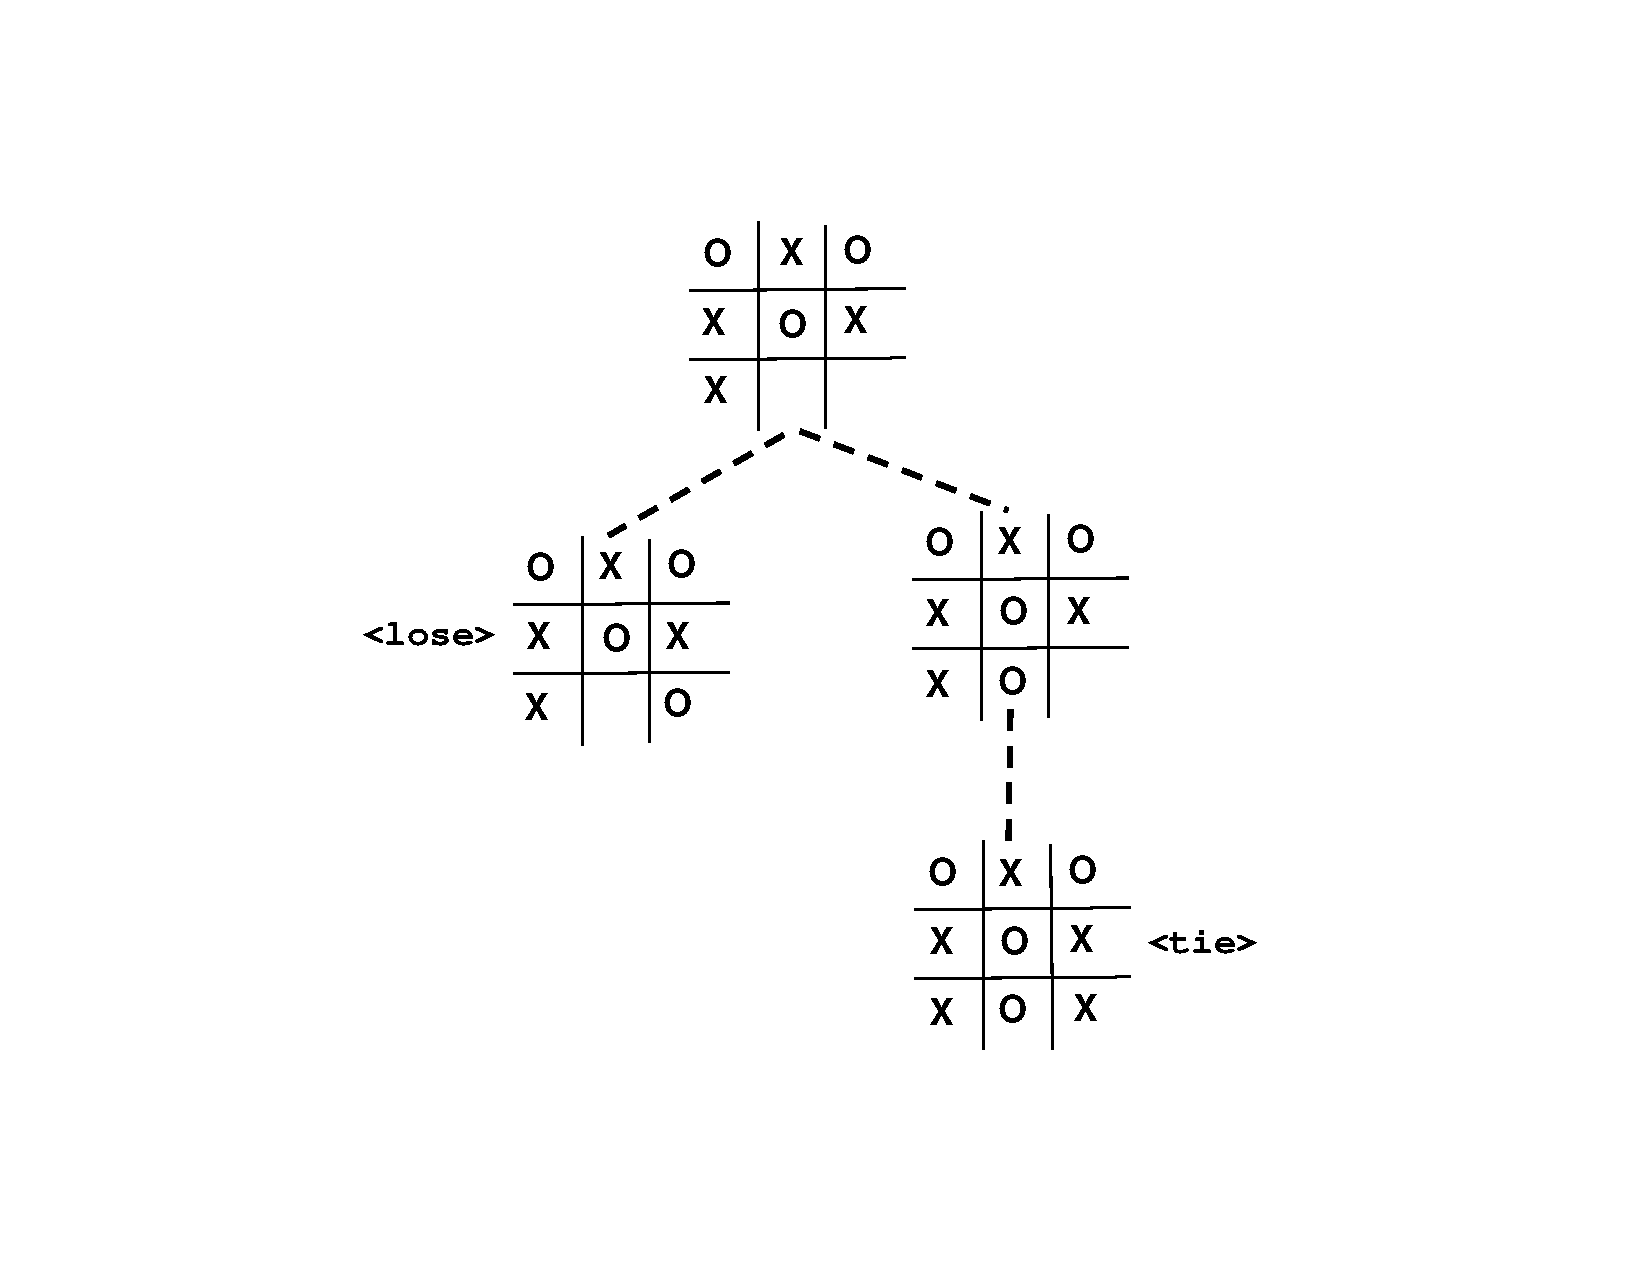
\includegraphics[height=4in]{figures/endgame.pdf}
\caption{Game Tree for the Tic-Tac-Toe game starting at $P_0$.}
\label{fig:endgame}
\end{figure}

Game trees are usually pictured in this way with the starting pattern
(referred to as the ``root'' of the tree) at the top and lines connecting
the root to the \iffalse roots of the \fi game trees that start at each
possible next pattern.  The ``leaves'' at the bottom of the tree (trees
grow upside down in Computer Science) correspond to terminated games.  A
path from the root to a leaf describes a complete \emph{play} of the game.
(In English, ``game'' can be used in two senses: first we can say that
Chess is a game, and second we can play a game of Chess.  The first usage
refers to the data type of Chess game trees, and the second usage refers to
a ``play.'')

\subsection{Infinite Tic-Tac-Toe Games}

At any point in a Tic-Tac-Toe game, there are at most nine possible next
patterns, and no play can continue for more than nine moves.  But suppose
we consider an \emph{$n$-game Tic-Tac-Toe tournament} where the tournament
winner is the one who wins more of $n>0$ individual Tic-Tac-Toe games.  (If
they each win an equal number of individual games, then the tournament is a
tie.)

Now we can consolidate all these tournaments into a single game we can call
\emph{Tournament-Tic-Tac-Toe}: the first player in Tournament-Tic-Tac-Toe
chooses any integer $n > 0$, and then the players play an $n$-game
tournament.  Now there are infinitely many possible first moves: the first
player can choose $n=1$, or $n=2$, or $n=3$, or \dots.  But still, it's
obvious that every possible play of Tournament-Tic-Tac-Toe is finite,
because after the first player chooses a value for $n$, the game can't
continue for more than $9n$ moves.  So it's not possible to keep playing
forever even though the game tree is infinite.

This isn't very hard to understand, but there is an important difference
between any given $n$-game tournament and Tournament-Tic-Tac-Toe: even
though every play of Tournament-Tic-Tac-Toe must come to an end, there is
no longer any bound on how many moves it might be before the game ends ---a
play might end after 9 moves, or $9(2001)$ moves, or $9(10^{10}+1)$ moves;
it just can't continue forever.

\iffalse While there is no bound on how long to play, at least after the
first move to an $n \times n$ board in meta-Tic-Tac-Toe, we know the game
will end with $n^2$ moves.\fi

With Tournament-Tic-Tac-Toe recognized as a \tg, we can go on to
Tournament$^2$-Tic-Tac-Toe where the first player chooses a number, $m>0$,
of Tournament-Tic-Tac-Toe games to play, and the second player acts as the
first player in each of the $m$ Tournament-Tic-Tac-Toe games to be played.
Then, of course, there's Tournament$^3$-Tic-Tac-Toe\dots.

\iffalse Every play of the meta-meta game must still end, but now even
after the first move, there is no bound on how long a game might
continue.\fi

\subsection{Two Person Terminating Games}

Familiar games like Tic-Tac-Toe, Checkers, and Chess can all end in ties,
but for simplicity we'll only consider win/lose games ---no ``everybody
wins''-type games at MIT. \texttt{:-)}.  But everything we show about
win/lose games will extend easily to games with ties.

\iffalse
Of course Tic-Tac-Toe and the
other games will fit this set up if we treat a game that ends in a tie as
a loss for the usual first player ---White in Chess, Red in Checkers, the
X-player in Tic-Tac-Toe.
\fi

Like Tic-Tac-Toe, the idea behind the definition of $\tg$'s as a
recursive data type is that making a move in a $\tg$ leads to the
start of a subgame.  In other words, given any set of games, we can
make a new game whose first move is to pick a game to play from the set.

So what defines a game?  For Tic-Tac-Toe, we used the patterns and the
rules of Tic-Tac-Toe to determine the next patterns.  But once we have
a complete game tree, we don't really need the pattern labels: the
root of a game tree itself can play the role of a ``board position''
with its possible ``next positions'' determined by the roots of its
subtrees.  So any game is defined by its game tree.  This leads to the
following very simple ---perhaps deceptively simple ---general
definition.

\begin{definition}
The \hyperdef{2p}{tg}{$\tg$}, \emph{game trees for two-person terminating
    games of perfect information} are defined recursively as follows:
\begin{itemize}

\item \textbf{Base cases:}
\[\begin{array}{ll}
\ang{\texttt{leaf},\texttt{win}} & \in \tg, \text{ and}\\
\ang{\texttt{leaf},\texttt{lose}}& \in \tg.
\end{array}\]

\item \textbf{Constructor case:}
If $\mathcal{G}$ is a nonempty set of
$\tg$'s, then $G$ is a $\tg$, where
\[
G \eqdef \ang{\texttt{tree},\mathcal{G}}.
\]
The game trees in $\mathcal{G}$ are called the possible \emph{next moves}
from $G$.
\end{itemize}

\end{definition}

These games are called ``terminating'' because, even though a $\tg$ may be
a (very) infinite datum like Tournament$^2$-Tic-Tac-Toe, every play of a
$\tg$ must terminate.  This is something we can now prove, after we give a
precise definition of ``play'':

\begin{definition}
A \emph{play} of a $\tg$, $G$, is a (potentially infinite) sequence of
$\tg$'s starting with $G$ and such that if $G_1$ and $G_2$ are consecutive
$\tg$'s in the play, then $G_2$ is a possible next move of $G_1$.

If a $\tg$ has no infinite play, it is called a \emph{terminating} game.
\end{definition}

\begin{theorem}
Every $\tg$ is terminating.
\end{theorem}

\begin{proof}
By structural induction on the definition of a $\tg$, $G$, with induction
hypothesis
\[
G \text{ is terminating}.
\]

\textbf{Base case}: If $G = \ang{\texttt{leaf}, \texttt{win}}$ or $G =
\ang{\texttt{leaf}, \texttt{lose}}$ then the only possible play of $G$ is
the length one sequence consisting of $G$.  Hence $G$ terminates.

\textbf{Constructor case}: For $G = \ang{\texttt{tree},\mathcal{G}}$, we
must show that $G$ is terminating, given the Induction Hypothesis that
\emph{every} $G' \in \mathcal{G}$ is terminating.

But any play of $G$ is, by definition, a sequence starting with $G$ and
followed by a play starting with some $G_0 \in \mathcal{G}$.  But $G_0$ is
terminating, so the play starting at $G_0$ is finite, and hence so is the
play starting at $G$.

This completes the structural induction, proving that every \tg, $G$, is
terminating.
\end{proof}


\subsection{Game Strategies}

A key question about a game is whether a player has a winning strategy.  A
\emph{strategy} for a player in a game specifies which move the player
should make at any point in the game.  A \emph{winning} strategy ensures
that the player will win no matter what moves the other player makes.

In Tic-Tac-Toe for example, most elementary school children figure out
strategies for both players that each ensure that the game ends with no
tic-tac-toes, that is, it ends in a tie.  Of course the first player can
win if his opponent plays childishly, but not if the second player follows
the proper strategy.  In more complicated games like Checkers or Chess,
it's not immediately clear that anyone has a winning strategy, even if we
agreed to count ties as wins for the second player.

But structural induction makes it easy to prove that in any $\tg$,
\emph{somebody} has the winning strategy!

\begin{theorem}\label{fund}
\textbf{Fundamental Theorem for Two-Person Games:} For every two-person
terminating game of perfect information, there is a winning strategy for
one of the players.
\end{theorem}

\begin{proof}
The proof is by structural induction on the definition of a $\tg$, $G$.
The induction hypothesis is that there is a winning strategy for $G$.

\textbf{Base cases:}
\begin{enumerate}

\item $G=\ang{\texttt{leaf}, \texttt{win}}$.  Then the first player has the
 winning strategy: ``make the winning move.''

\item $G=\ang{\texttt{leaf}, \texttt{lose}}$.  Then the second player has a
 winning strategy: ``Let the first player make the losing move.''
\end{enumerate}

\textbf{Constructor case}: Suppose $G = \ang{\texttt{tree},\mathcal{G}}$.
By structural induction, we may assume that some player has a winning
strategy for each $G' \in \mathcal{G}$.  There are two cases to consider:
\begin{itemize}
\item some $G_0 \in \mathcal{G}$ has a winning strategy for its second
  player.  Then the first player in $G$ has a winning strategy: make the
  move to $G_0$ and then follow the second player's winning strategy in
  $G_0$.

\item every $G' \in \mathcal{G}$ has a winning strategy for its first
  player.  Then the second player in $G$ has a winning strategy: if the
  first player's move in $G$ is to $G_0 \in \mathcal{G}$, then follow the
  winning strategy for the first player in $G_0$.
\end{itemize}
So in any case, one of the players has a winning strategy for $G$, which
completes the proof of the constructor case.

It follows by structural induction that there is a winning strategy for
every $\tg$, $G$.
\end{proof}

Notice that although Theorem~\ref{fund} guarantees a winning strategy, its
proof gives no clue which player has it.  For
\iffalse the Subset Takeaway Game
(\href{http://courses.csail.mit.edu/6.042/fall07/rec3t.pdf} {Recitation
Problem, Tuesday, Week 3}), and
\fi
most familiar $\tg$'s like Chess, Go, \dots, no one knows
which player has a winning strategy.\footnote{Checkers used to be in this
  list, but there has been a recent announcement that each player has a
  strategy that forces a tie. (reference TBA}

%% Games as a Recursive Data Type Problems %%%%%%%%%%%%%%%%%%%%%%%%%%%%%%%%%%%%
%\startclassproblems


%% Induction in Computer Science %%%%%%%%%%%%%%%%%%%%%%%%%%%%%%%%%%%%%%%%%%%%%%
\section{Induction in Computer Science}

Induction is a powerful and widely applicable proof technique, which is why
we've devoted an entire chapter to it.  Strong induction and its special
case of ordinary induction are applicable to any kind of thing with
nonnegative integer sizes --which is a awful lot of things, including all
step-by-step computational processes.

\iffalse
Ordinary induction is specially helpful in the study of computation.  Why?
Well, ordinary induction on nonnegative integers is a ``one step at a
time'' proof method.  Computations also evolve ``one step at a time.''
\fi

Structural induction then goes beyond natural number counting by offering a
simple, natural approach to proving things about recursive computation
and recursive data types.  This makes it a technique every Computer
Scientist should embrace.

\iffalse
In many cases a nonnegative integer size can be defined for a recursively
defined datum, such as the length of a string, or the number of operations
in an $\aexp$.  It is then possible to prove properties of data by ordinary
induction on their size.  But this approach often produces more cumbersome
proofs than structural induction.

In fact, structural induction is theoretically more powerful than ordinary
induction.  However, it's only more powerful when it comes to reasoning
about infinite data types ---like infinite trees, for example ---so this
greater power doesn't matter in practice.  What does matter is that for
recursively defined data types, structural induction is a simple and
natural approach.
\fi

\endinput
 %structural induction, Ackermann function, while
                         %programs, Hoare logic, games  *Albert
%%% Jay: there is some commented out material in ln3 about games wrt PO's

%\documentclass[handout]{mcs}

\begin{document}

\inclassproblems{6, Mon.}

%%%%%%%%%%%%%%%%%%%%%%%%%%%%%%%%%%%%%%%%%%%%%%%%%%%%%%%%%%%%%%%%%%%%%
% Problems start here
%%%%%%%%%%%%%%%%%%%%%%%%%%%%%%%%%%%%%%%%%%%%%%%%%%%%%%%%%%%%%%%%%%%%%

\begin{staffnotes}
Infinite Cardinality;  Ch. 8.1.1--8.1.3
\end{staffnotes}

\pinput{CP_countable_surjection-alt}

\pinput{CP_rationals_are_countable}
\hint Use Problem 1.

%\pinput{FP_uncountable_infinite_sequences}

\pinput{CP_smallest_infinite_set}

\pinput{PS_unit_interval}

\begin{center}
\textbf{Supplemental (Optional)}
\end{center}
\pinput{CP_Schroeder_Bernstein_theorem}  %more suited for pset




%%%%%%%%%%%%%%%%%%%%%%%%%%%%%%%%%%%%%%%%%%%%%%%%%%%%%%%%%%%%%%%%%%%%%
% Problems end here
%%%%%%%%%%%%%%%%%%%%%%%%%%%%%%%%%%%%%%%%%%%%%%%%%%%%%%%%%%%%%%%%%%%%%
\end{document}

%\input{cp6t}
%\input{cp6r}
%\documentclass[handout]{mcs}

\begin{document}

\inclassproblems{7, Mon.}

%%%%%%%%%%%%%%%%%%%%%%%%%%%%%%%%%%%%%%%%%%%%%%%%%%%%%%%%%%%%%%%%%%%%%
% Problems start here
%%%%%%%%%%%%%%%%%%%%%%%%%%%%%%%%%%%%%%%%%%%%%%%%%%%%%%%%%%%%%%%%%%%%%
%from S11 cp6w:

\pinput{CP_de_Bruijn_graphs}
\pinput{CP_covering_edges}
\pinput{CP_walk_relation_composition}


\iffalse
%\pinput{CP_directed_walks_and_cycles}
\pinput{CP_de_Bruijn_graphs}
\pinput{CP_tournament_chain}
%\pinput{CP_covering_edges}
\pinput{PS_walk_relation_composition}
\fi



%%%%%%%%%%%%%%%%%%%%%%%%%%%%%%%%%%%%%%%%%%%%%%%%%%%%%%%%%%%%%%%%%%%%%
% Problems end here
%%%%%%%%%%%%%%%%%%%%%%%%%%%%%%%%%%%%%%%%%%%%%%%%%%%%%%%%%%%%%%%%%%%%%
\end{document}



%\documentclass[handout]{mcs}

\begin{document}

\renewcommand{\reading}
{
  \emph{For this pset}:
  Sections~\bref{Turing_sec}{--}\bref{mod_prime_sec}{ on Modular Arithmetic}, and
  Sections~\bref{arithmetic_modn_sec}{ on Euler's Theorem}.
  %Section~\bref{state_machine_sec}{ on State Machines}, 
  %Chapter~\bref{recursive_data_chap}{ on Recursive Data}, and 
  %Sections~\bref{divisibility_sec}{--}
  %  ~\bref{fundamental_theorem_sec}{ on Number Theory.}

\emph{For lecture, Friday, Oct. 14}:
Sections~\bref{RSA_sec}{--}\bref{SAT_RSA-sec}{ on The RSA crypto-system}.
%Section~\bref{Turing_sec}{--}~\bref{mod_prime_sec}{ on Modular Arithmetic.}
}

\problemset{5}


\emph{Reminders}:
\begin{itemize}
\item The final deadline for Online Tutor Problems TP.6 and a
  \href{http://courses.csail.mit.edu/6.042/fall11/courseinfo#comments}{Piazza
    comment} on the reading is Thursday, Oct. 13, 10PM.
\iffalse
\item Problems should be submitted separately following the pset
  \href{http://courses.csail.mit.edu/6.042/fall11/submission}{submission
    instructions}, and each problem should have a \emph{collaboration
    statement} at the beginning, with the requisite information
  written in or attached using the
  \href{http://courses.csail.mit.edu/6.042/fall11/submission_template.pdf}{collaboration
    statement template}.
\fi

\end{itemize}


%TOPICS: state machines invariance, recursive data, GCD's

%%%%%%%%%%%%%%%%%%%%%%%%%%%%%%%%%%%%%%%%%%%%%%%%%%%%%%%%%%%%%%%%%%%%%
% Problems start here
%%%%%%%%%%%%%%%%%%%%%%%%%%%%%%%%%%%%%%%%%%%%%%%%%%%%%%%%%%%%%%%%%%

% PSET PROBLEMS FOR WEEK 5 FRIDAY
\pinput{PS_calculating_inverses} % I can change the numbers if necessary.

%\pinput{PS_self-inverse_mod_p} % Should remove all mention of the theorem name; move it to the solution
                               % so students don't just look up the proof.
%\pinput{CP_polynomials_produce_multiples} % New to repo; hints and restructuring may be in order.

% PSET PROBLEMS FOR WEEK 6 WEDNESDAY
%cp6w + mq7m: \pinput{PS_Euler_theorem_calculation}
%reject: \pinput{CP_13th_roots}
\pinput{FP_modular_powerful}
\pinput{PS_Euler_function_multiplicativity}

%mq7m: \pinput{TP_Relative_Primality}

% PSET PROBLEMS FOR WEEK 6 FRIDAY
%cp6f: \pinput{PS_RSA_correctness}
%reject: \pinput{PS_RSA_key_implies_factoring}
%reject: \pinput{PS_Rabin_cryptosystem}

% CLASS PROBLEMS FOR WEEK 6 WEDNESDAY
%\pinput{PS_Euler_theorem_calculation}
%\pinput{PS_congruent_modulo_1000}
%\pinput{CP_chinese_remainder}
%\pinput{PS_Euler_function_multiplicativity}

% CLASS PROBLEMS FOR WEEK 6 FRIDAY
%\pinput{CP_RSA_between_tables}
%\pinput{CP_RSA_proving_correctness}

% MINIQUIZ PROBLEMS: MORNING
%\pinput[points = 5]{MQ_Euler_function_of_100}
%\pinput[points = 5]{TP_Relative_Primality_6042}
%\pinput[points = 5]{FP_Euler_theorem_calculation}
%\pinput[points = 5]{TP_Eulers_Theorem}

% MINIQUIZ PROBLEMS: AFTERNOON
%\pinput[points = 5]{MQ_Euler_function_of_6042}
%\pinput[points = 5]{TP_Relative_Primality}

% COPIED FROM spring11/ps5.tex
%%\pinput{CP_conquering_the_galaxy}
%%\pinput{PS_directed_Euler_circuits}
%\pinput{CP_binary_relations_on_01}
%\pinput{PS_top_sort_for_closure_of_DAG}
%\pinput{PS_Brents_theorem}
%%\pinput{CP_product_relation_properties}
%\pinput{PS_subsequences_partial_order_Dilworth_Lemma}
%%\pinput{PS_weak_partial_order_isomorphic_to_subset}

% COPIED FROM fall11/ps4.tex
%\pinput{CP_robot_invariant}
%\pinput{PS_bracket_good_count}
%\iffalse
%%NOT THIS WEEK
%\pinput{PS_calculating_inverses}
%\large\textbf{Repo: PS\_congruent\_modulo\_1000}
%\pinput{PS_congruent_modulo_1000}
%\large\textbf{Repo: PS\_RSA\_correctness}
%\pinput{PS_RSA_correctness}
%\fi
%%\large\textbf{Repo: CP\_binary\_trees}
%%\pinput{CP_binary_trees}
%\pinput{PS_linear_combination_by_structural_induction}
%\pinput{PS_labeled_binary_trees}
%%\large\textbf{Repo: PS\_linear\_combination\_game}
%%\pinput{PS_linear_combination_game}

%%%%%%%%%%%%%%%%%%%%%%%%%%%%%%%%%%%%%%%%%%%%%%%%%%%%%%%%%%%%%%%%%%%%%
% Problems end here
%%%%%%%%%%%%%%%%%%%%%%%%%%%%%%%%%%%%%%%%%%%%%%%%%%%%%%%%%%%%%%%%%%%%%
\end{document}


\chapter{Simple Graphs}
%\coursecopyright

%% Introduction %%%%%%%%%%%%%%%%%%%%%%%%%%%%%%%%%%%%%%%%%%%%%%%%%%%%%%%%%%%%%%%
Graphs arise in different fields with all sorts of applications,
including scheduling, optimization, communications, and the design and
analysis of algorithms.  Two Stanford students even used graph theory to
become multibillionaires!

But we'll start with an application designed to get your attention: we are
going to make a professional inquiry into sexual behavior.  Namely, we'll
look at some data about who, on average, who has more opposite-gender
partners, men or women?

Sexual demographics have been the subject of many studies.  In one of the
largest, researchers from the University of Chicago interviewed a random
sample of 2500 people over several years to try to get an answer to this
question.  Their study, published in 1994, and entitled \emph{The Social
  Organization of Sexuality} found that on average men have 74\% more
opposite-gender partners than women.

Other studies have found that the disparity is even larger.  In
particular, ABC News claimed that the average man has 20 partners over his
lifetime, and the average woman has 6, for a percentage disparity of
233\%.  The ABC News study, aired on Primetime Live in 2004, purported to
be one of the most scientific ever done, with only a 2.5\% margin of
error.  It was called "American Sex Survey: A peak between the sheets,"
---which makes its science start to sound a little doubtful.  \iffalse The
promotion for the study is even better:
\begin{quote} 
A ground breaking ABC News ``Primetime Live'' survey finds a range of
eye-popping sexual activities, fantasies and attitudes in this country,
confirming some conventional wisdom, exploding some myths -- and venturing
where few scientific surveys have gone before.
\end{quote}
Probably that last part about going where few scientific surveys have gone
before is pretty accurate!
\fi
Yet again, in August, 2007, the N.Y. Times
\href{http://www.nytimes.com/2007/08/12/weekinreview/12kolata.html?_r=1&n=Top/Reference/Times%20Topics/People/K/Kolata,%20Gina&oref=slogin}{reported} on a study by the
  National Center for Health Statistics of the U.S. government showing
  that men had seven partners while women had four.

  Anyway, whose numbers do you think are more accurate, the University of
  Chicago, ABC News, or the National Center?  Don't answer: this is a setup
  question like ``When did you stop beating your wife?''  Using a little
  graph theory, we'll explain why none of these findings can be anywhere
  near the truth.


%% Simple Graphs %%%%%%%%%%%%%%%%%%%%%%%%%%%%%%%%%%%%%%%%%%%%%%%%%%%%%%%%%%%%%%
\hyperdef{simple}{graphs}{\section{Simple Graphs}}

\subsection{Definition of Simple Graph}

Informally, a graph is a bunch of dots with lines connecting some of
them.  Here is an example:

\mfigure{!}{1.5in}{figures/graph-example.pdf}

For many Mathematical purposes, we don't really care how the points and
lines are laid out ---only which points are connected by lines.  The
definition of \emph{simple graphs} aims to capture just this connection
data.

\begin{definition}\label{graphdef} 
A \emph{simple graph}, $G$, consists of a nonempty set, $V$, called the
\emph{vertices} of $G$, and a collection, $E$, of two-element subsets of
$V$.  The members of $E$ are called the \emph{edges} of $G$.
\end{definition}

The vertices correspond to the dots in the picture, and the edges
correspond to the lines.  For example, the connection data in
dots-and-lines diagram above is a captured by the following simple graph:
\begin{eqnarray*}
V & = & \set{A, B, C, D, E, F, G, H, I} \\
E & = & \set{ \set{A, B}, \set{A, C}, \set{B, D}, \set{C, D},
              \set{C, E}, \set{E, F}, \set{E, G}, \set{H, I} }.
\end{eqnarray*}

It will be helpful to use the notation $\edge{A}{B}$ for the edge
$\set{A,B}$.  Note that $\edge{A}{B}$ and $\edge{B}{A}$ are different
descriptions of the same edge, since sets are unordered.

Two vertices in a simple graph are said to be \term{adjacent} if they are
joined by an edge, and an edge is said to be \term{incident} to the
vertices it joins.  The number of edges incident to a vertex is called the
\term{degree} of the vertex; equivalently, the degree of a vertex is
equals the number of vertices adjacent to it.  For example, in the simple
graph above, $A$ is adjacent to $B$ and $B$ is adjacent to $D$, and the
edge $\edge{A}{C}$ is incident to vertices $A$ and $C$.  Vertex $H$ has
degree 1, $D$ has degree 2, and $E$ has degree 3.

\subsubsection{Graph Synonyms}

A synonym for ``vertices'' is "nodes,'' and we'll use these words
interchangeably.

Simple graphs are sometimes called \emph{networks}, edges are sometimes
called \emph{arcs}, and adjacent vertices are sometimes called
\emph{neighbors}.  We mention this as a ``heads up'' in case you look at
other graph theory literature; we won't use these words.

Some technical consequences of Definition~\ref{graphdef} are worth noting
right from the start:
\begin{enumerate}
\item Simple graphs do not have edges going from a vertex
back around to itself (called a \emph{self-loop}).

\item There is at most one edge between two vertices of a simple graph.

\item Simple graphs have at least one vertex, though they might not have
any edges.
\end{enumerate}
There's no harm in relaxing these conditions, and some authors do, but we
don't need self-loops, multiple edges between the same two vertices, or
graphs with no vertices, and it's simpler not to have them around.

For the rest of these Notes we'll only be considering simple graphs, so
we'll just call them ``graphs'' from now on.

\hyperdef{sex}{america}{\subsection{Sex in America}\label{sexam}}

%A 1994 University of Chicago study entitled \textit{The Social
%Organization of Sexuality} found that on average men have 74\% more
%opposite-gender partners than women.

Let's model the question of heterosexual partners in graph theoretic
terms.  To do this, we'll let $G$ be the graph whose vertices, $V$, are
all the people in America.  Then we split $V$ into two separate subsets:
$M$, which contains all the males, and $F$, which contains all the
females.\footnote{For simplicity, we'll ignore the possibility of someone
  being both, or neither, a man and a woman.}  We'll put an edge between a
male and a female iff they have been sexual partners.  This graph is
pictured in Figure~\ref{fig:partners} with males on the left and females on
the right.

\begin{figure}[htbp]
\centering 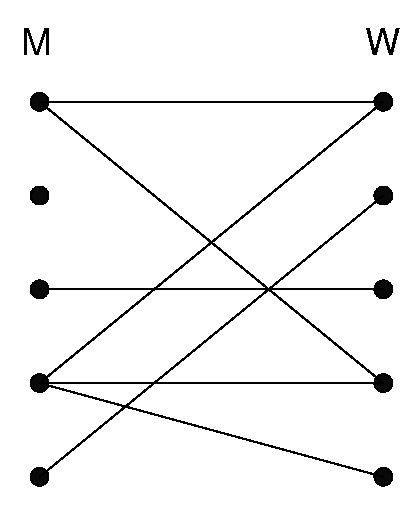
\includegraphics[height=1.75in]{figures/sex-edges.pdf}
\caption{The sex partners graph}
\label{fig:partners}
\end{figure}

Actually, this is a pretty hard graph to figure out, let alone draw.  The
graph is \emph{enormous}: the US population is about 300 million, so
$\card{V} \approx 300M$!  Of these, approximately 50.8\% are female and
49.2\% are male, so $\card{M} \approx 147.6M$, and $\card{F} \approx
152.4M$.  And we don't even have trustworthy estimates of how many edges
there are, let alone exactly which couples are adjacent.

But it turns out that we don't need to know any of this ---we just need to
figure out the relationship between the average number of partners per
male and partners per female.  To do this, we note that every edge is
incident to exactly one $M$ vertex (remember, we're only considering
male-female relationships); so the sum of the degrees of the $M$ vertices
equals the number of edges.  For the same reason, the sum of the degrees
of the $F$ vertices equals the number of edges.  So these sums are equal:
%
\[
\sum_{x \in M} \degr{x} = \sum_{y \in F} \degr{y}.
\]
%
Now suppose we divide both sides of this equation by the product of
the sizes of the two sets, $\card{M} \cdot \card{F}$:
%
\[
\left(\frac{\sum_{x \in M} \degr{x}}{\card{M}}\right) \cdot \frac{1}{\card{F}} =
\left(\frac{\sum_{y \in F} \degr{y}}{\card{F}}\right) \cdot \frac{1}{\card{M}}
\]
%
The terms above in parentheses are the \textit{average degree of an $M$
vertex} and the \textit{average degree of a $F$} vertex.  So we know:
\[
\text{Avg. deg in $M$} = \frac{\card{F}}{\card{M}} \cdot \text{Avg. deg in $F$}
\]

In other words, we've proved that the average number of female partners of
males in the population compared to the average number of males per
female is \emph{determined solely by the relative number of males and
females in the population}.

Now the Census Bureau reports that there are slightly more females than
males in America; in particular $\card{F} / \card{M}$ is about 1.035.  So
we know that on average, males have 3.5\% more opposite-gender partners
than females, and this tells us nothing about any sex's promiscuity or
selectivity.  Rather, it just has to do with the relative number of males
and females.  Collectively, males and females have the same number of
opposite gender partners, since it takes one of each set for every
partnership, but there are fewer males, so they have a higher ratio.  So the
University of Chicago, ABC, and the Federal government studies are way
off.  After a huge effort, they gave a totally wrong answer.

There's no definite explanation for why such surveys are consistently
wrong.  One hypothesis is that males exaggerate their number of partners
---or maybe females downplay theirs ---but these explanations are
speculative.  Interestingly, the principal author of the National Center
for Health Statistics study reported that she knew the results had to be
wrong, but that was the data collected and her job was to report that.

The same underlying issue has led to serious misinterpretations of other
survey data.  For example, a couple of years ago, the Boston Globe ran a
story on a survey of the study habits of students on Boston area campuses.
Their survey showed that on average, minority students tended to study
with non-minority students more than the other way around.  They went on
at great length to explain why this ``remarkable phenomenon'' might be
true.  But it's not remarkable at all ---using our graph theory
formulation, we can see that all it says is that there are fewer minority
students than non-minority students.  Well, that just follows from the
definition of ``minority''!

\subsection{Handshaking Lemma}

The previous argument hinged on the connection between a sum of degrees
and the number edges.  There is a simple connection between these in any
graph:

\begin{theorem}\label{sumedges}
The sum of the degrees of the vertices in a graph equals twice the number
of edges.
\end{theorem}

\begin{proof}
Every edge contributes two to the sum of the degrees, one for each of its
endpoints.
\end{proof}

Theorem~\ref{sumedges} is sometimes called the \emph{Handshake Theorem}:
if we total up the number of people each person at a party shakes hands
with, the total will be twice the number of handshakes that occurred.

\subsection{Some Common Graphs}

Some graphs come up so frequently that they have names.  The {\em complete
graph} on $n$ vertices, also called $K_n$, has an edge between every two
vertices.  Here is $K_5$:

\mfigure{!}{1.5in}{figures/complete-graph.pdf}

The {\em empty graph} has no edges at all.  Here is the
empty graph on 5 vertices:

\mfigure{!}{1.5in}{figures/empty-graph.pdf}

Another 5 vertex graph is $L_4$, the \emph{line graph} of length four:

\mfigure{!}{1in}{figures/path-graph.pdf}

And here is $C_5$, a \emph{simple cycle} with 5 vertices:

\mfigure{!}{1.5in}{figures/cycle.pdf}

\subsection{Isomorphism}

Two graphs that look the same might actually be different in a formal
sense.  For example, the two graphs below are both simple cycles with
4~vertices:

\mfigure{!}{1.5in}{figures/isomorphism.pdf}

But one graph has vertex set $\set{A, B, C, D}$ while the
other has vertex set $\set{1, 2, 3, 4}$.  If so, then the graphs are
different mathematical objects, strictly speaking.  But this is a
frustrating distinction; the graphs {\em look the same}!

Fortunately, we can neatly capture the idea of ``looks the same.''  Graphs
$G_1$ and $G_2$ are {\em isomorphic} if there exists a bijection between
the vertices in $G_1$ and the vertices in $G_2$ such that there is an edge
between two vertices in $G_1$ if and only if there is an edge between the
two corresponding vertices in $G_2$.  For example, take the following
bijection between vertices in the two graphs above:
\[
\begin{array}{lll}
A \text{ corresponds to } 1 & \hspace{0.5in} & B \text{ corresponds to } 2 \\
D \text{ corresponds to } 4 & & C \text{ corresponds to } 3.
\end{array}
\]
Now there is an edge between two vertices in the graph on the left if and
only if there is an edge between the two corresponding vertices in the
graph on the right.  Therefore, the two graphs are isomorphic.  The
bijection itself is called an {\em isomorphism}.
\begin{definition}
If $G_1$ is a graph with vertices, $V_1$, and edges,
$E_1$, and likewise for $G_2$, then $G_1$ is {\em isomorphic} to $G_2$ iff
there exists a \textbf{bijection}, $f: V_1 \to V_2$, such that for
every pair of vertices $u, v \in V_1$:
\[
\edge{u}{v} \in E_1 \qiff \edge{f(u)}{f(v)} \in E_2.
\]
The function $f$ is called an {\em isomorphism} between $G_1$ and
$G_2$.
\end{definition}

Two isomorphic graphs may be drawn very differently.  For example, here
are two different ways of drawing $C_5$:

\mfigure{!}{1.5in}{figures/isomorphism-c5.pdf}

Isomorphism captures all the connection properties of a graph, abstracting
out what the vertices are called, what they are made out of, or where they
appear in a drawing of the graph.  So a property like ``having three
vertices of degree 4'' is preserved under isomorphism, while ``having a
vertex that is an integer'' is not preserved.  In particular, if one graph
has three vertices of degree 4 and another does not, they can't be
isomorphic.  Similarly, if one graph has an edge that is incident to
a degree 8 vertex and a degree 3 vertex, then any isomorphic graph must also
have such an edge.

Looking for properties like these can make it easy to determine that two
graphs are not isomorphic, or to actually find an isomorphism between
them, if there is one.  In practice, it's frequently easy to decide
whether two graphs are isomorphic.  However, no one has yet found a
\emph{general} procedure for determining whether two graphs are isomorphic
which is \emph{guaranteed} to run much faster than an exhaustive (and
exhausting) search through all possible bijections between their
vertices.

Having an efficient procedure to detect isomorphic graphs would, for
example, make it easy to search for a particular molecule in a database
given the molecular bonds.  On the other hand, knowing there is no such
efficient procedure would also be valuable: secure protocols for
encryption and remote authentication can be built on the hypothesis that
graph isomorphism is computationally exhausting.

%% Simple Graphs Problems %%%%%%%%%%%%%%%%%%%%%%%%%%%%%%%%%%%%%%%%%%%%%%%%%%%%%
%\startclassproblems
%\pinput{CP_handshaking_proofs}
%\pinput{CP_isomorphism_finger_exercise}
%\pinput{CP_neighbors_under_isomorphism}
% S09.cp6m.1
% S09.cp6m.3
% S09.cp6m.4


%% Connectedness %%%%%%%%%%%%%%%%%%%%%%%%%%%%%%%%%%%%%%%%%%%%%%%%%%%%%%%%%%%%%%
\hyperdef{connect}{edness}{\section{Connectedness}}

\subsection{Paths and Simple Cycles}

A \emph{path} in a graph describes how to get from one vertex to another
following edges of the graph.  Formally,

\begin{definition}
A \term{path} in a graph, $G$, is a sequence of $k \geq 0$ vertices
\[
v_0,\dots,v_k
\]
such that $\edge{v_i}{v_{i+1}}$ is an edge of $G$ for all $i$ where $0
\leq i < k$ .  The path is said to \term{start} at $v_0$, to \term{end} at
$v_k$, and \term{length} of the path is defined to be $k$.  An edge,
$\edge{u}{v}$, is \term{traversed $n$ times} by the path if there are $n$
different values of $i$ such that $\edge{v_i}{v_{i+1}} = \edge{u}{v}$.

The path is \term{simple}\footnote{Heads up if you read another graph
  theory text: what amounts to paths are commonly referred to as
  ``walks,'' and simple paths are referred to as a just ``paths''.
  Likewise, what we will call \emph{cycles} and \emph{simple cycles}
  are commonly called ``closed walks'' and just ``cycles''.}  iff all
the $v_i$'s are different, that is, $v_i = v_j$ only if $i=j$.

\end{definition}

For example, the graph in Figure~\ref{dg} has a length~6 simple path
A,B,C,D,E,F,G.  This is the longest simple path in the graph.

\begin{figure}[htbp] 
\mfigure{!}{1.75in}{figures/distance-graph.pdf}
\caption{\em A graph with 3 simple cycles.}
\label{dg}
\end{figure}

Notice that the {\em length} of a path is the total number of times it
traverses edges, which is \emph{one less} than its length as a sequence of
vertices.  The length~6 path A,B,C,D,E,F,G is actually a sequence of seven
vertices.

A \emph{cycle} can be described by a path \iffalse of length two or
more\fi that begins and ends with the same vertex.  For example,
B,C,D,E,C,B is a cycle in the graph in Figure~\ref{dg}.  This path
suggests that the cycle begins and ends at vertex B, but a cycle isn't
intended to have a beginning and end, and can be described by \emph{any}
of the paths that go around it.  For example, D,E,C,B,C,D describes this
same cycle as though it started and ended at D, and D,C,B,C,E,D describes
the same cycle as though it started and ended at D but went in the
opposite direction.  (By convention, a single vertex is a length 0 cycle
beginning and ending at the vertex.)

All the paths that describe the same cycle have the same length which is
defined to be the {\em length} of the cycle.  (Note that this implies that
going around the same cycle twice is considered to be different than going
around it once.)

A \emph{simple} cycle is a cycle that doesn't cross or backtrack on
itself.  For example, the graph in Figure~\ref{dg} has three simple cycles
B,H,E,C,B and C,D,E,C and B,C,D,E,H,B.  More precisely, a simple cycle is
a cycle that can be described by a path of length at least three whose
vertices are all different except for the beginning and end vertices.  So
in contrast to simple \emph{paths}, the length of a simple \emph{cycle} is
the \emph{same} as the number of distinct vertices that appear in it.

From now on we'll stop being picky about distinguishing a cycle from a
path that describes it, and we'll just refer to the path as a cycle.
\footnote{Technically speaking, we haven't ever defined what a cycle
\emph{is}, only how to describe it with paths.  But we won't need an
abstract definition of cycle, since all that matters about a cycle is which
paths describe it.}

\iffalse

Simple cycles are especially important, so we will give a proper
definition of them.  Namely, we'll define a simple cycle in $G$ to be a
\emph{subgraph} of $G$ that looks like a cycle that doesn't cross itself.
Formally:

\begin{definition}
A \term{subgraph}, $G'$, of a graph, $G$, is a graph whose vertices, $V'$,
are a subset of the vertices of $G$ and whose edges are a subset
of the edges of $G$.
\end{definition}
Notice that since a subgraph is itself a graph, the endpoints of every
edge of $G'$ must be vertices in $V'$.

\begin{definition}
For $n \ge 3$, let $C_n$ be the graph with vertices $1,\dots, n$ and
edges
\[
\edge{1}{2},\ \ \edge{2}{3},\ \ \dots,\ \ \edge{(n-1)}{n},\ \ \edge{n}{1}.
\]
 graph is a \term{simple cycle of length $n$} iff it is isomorphic to
$C_n$ for some $n \ge 3$.  A \term{simple cycle of a graph}, $G$, is a
subgraph of $G$ that is a simple cycle.
\end{definition}
\fi


\subsection{Connected Components}

\begin{definition}
Two vertices in a graph are said to be \term{connected} if there is a path
that begins at one and ends at the other.
\end{definition}

By convention, every vertex is considered to be connected to itself by a
path of length zero.

\iffalse

Now if there is a path from vertex $u$ to vertex $v$, then $v$ is
connected to $u$ by the reverse path, so connectedness is a symmetric
relation.  Also, if there is a path from $u$ to $v$, and also a path from
$v$ to $w$, then these two paths can be combined to form a path from $u$
to $w$.  So the connectedness relation is transitive.  It is also
reflexive, since every vertex is by definition connected to itself by a
path of length zero.
\fi

The diagram in Figure~\ref{fig:3comp} looks like a picture of three
graphs, but is intended to be a picture of \emph{one} graph.  This graph
consists of three pieces (subgraphs).  Each piece by itself is connected,
but there are no paths between vertices in different pieces.

\iffalse
\begin{figure}[htbp]
\mfigure{!}{1.5in}{figures/3comp.pdf}
% \centerline{\psfig{figure=figures/3comp.eps,height=1.5in}}
\caption{\em One graph with 3 connected components.}
\label{fig:3comp}
\end{figure}
\fi

\begin{figure}[htbp] 
\mfigure{!}{1.5in}{figures/connectivity-graphs.pdf}
\caption{\em One graph with 3 connected components.}
\label{fig:3comp}
\end{figure}

\begin{definition}
A graph is said to be \term{connected} if every pair of vertices are
connected.
\end{definition}

These connected pieces of a graph are called its \term{connected
components}.  A rigorous definition is easy: a connected component is the
set of all the vertices connected to some single vertex.  So a graph is
connected iff it has exactly one connected component.  The empty graph on
$n$ vertices has $n$ connected components.

\subsection{How Well Connected?}

If we think of a graph as modelling cables in a telephone network, or oil
pipelines, or electrical power lines, then we not only want connectivity,
but we want connectivity that survives component failure.  A graph is
called \emph{$k$-edge connected} if it remains connected as long as fewer
than $k$ ``direct connections between components fail,'' that is, it stays
connected even if as many as $k-1$ edges are deleted.  More precisely:
\begin{definition}
  Two vertices in a graph are \term{$k$-edge connected} if they remain
  connected in every subgraph obtained by deleting $k-1$ edges.  A graph
  with at least two vertices is $k$-edge connected\footnote{The
    corresponding definition of connectedness based on deleting vertices
    rather than edges is common in Graph Theory texts and is usually
    simply called ``$k$-connected'' rather than ``$k$-vertex connected.''}
  if every two of its vertices are $k$-edge connected.
\end{definition}
So 1-edge connected is the same as connected for both vertices and graphs.
Another way to say that a graph is $k$-edge connected is that every
subgraph obtained from it by deleting at most $k-1$ edges is connected.

For example, in the graph in Figure~\ref{dg}, vertices B and E are
2-edge connected, G and E are 1-edge connected, and no vertices are 3-edge connected.
The graph as a whole is only 1-edge connected.

More generally, any simple cycle is 2-edge connected, and the complete graph,
$K_n$, is $(n-1)$-edge connected.

If two vertices are connected by $k$ edge-disjoint paths (that is, no two
paths traverse the same edge), then they are obviously $k$-edge connected.
A fundamental fact, whose ingenious proof we omit, is Menger's theorem
which confirms that the converse is also true: if two vertices are
$k$-edge connected, then there are $k$ edge-disjoint paths connecting
them.  It takes some ingenuity to prove this even for the case $k=2$.




\subsection{Connection by Simple Path}

Where there's a path, there's a simple path.  This is sort of obvious, but
it's easy enough to prove rigorously using the Well-ordering Principle.

\begin{lemma}\label{simplepath}
If vertex $u$ is connected to vertex $v$ in a graph, then there is a
simple path from $u$ to $v$.
\end{lemma}

\begin{proof}
Since there is a path from $u$ to $v$, there must, by the Well-ordering
Principle, be a minimum length path from $u$ to $v$.  If the minimum
length is zero or one, this minimum length path is itself a simple path
from $u$ to $v$.

Otherwise, there is a minimum length path
\[
v_0, v_1,\dots, v_k
\]
from $u = v_0$ to $v = v_k$ where $k \geq 2$.  We claim this path must be
simple.

To prove the claim, suppose to the contrary that the path is not simple,
that is, some vertex on the path occurs twice.  This means that there are
integers $i,j$ such that $0 \leq i < j \leq k$ with $v_i= v_j$.  Then
deleting the subsequence
\[
v_{i+1}, \dots v_j
\]
yields a strictly shorter path
\[
v_0, v_1,\dots, v_i,v_{j+1},v_{j+2},\dots, v_k
\]
from $u$ to $v$, contradicting the minimality of the given path.
\end{proof}

Actually, we proved something stronger:
\begin{corollary}\label{ss}
For any path of length $k$ in a graph, there is a simple path of length
\emph{at most} $k$ with the same endpoints.
\end{corollary}

\subsection{The Minimum Number of Edges in a Connected Graph}

The following theorem says that a graph with few edges must have many
connected components.

\begin{theorem} \label{th:connectivity}
Every graph with $v$ vertices and $e$ edges has at least $v - e$ connected
components.
\end{theorem}

Of course for Theorem~\ref{th:connectivity} to be of any use, there must
be fewer edges than vertices.

\begin{proof}
We use induction on the number of edges, $e$.  Let $P(e)$ be the
proposition that
\begin{quote}
for every $v$, every graph with $v$ vertices and $e$ edges has at least
$v-e$ connected components.
\end{quote}

\textbf{Base case:}($e=0$).  In a graph with 0 edges and $v$ vertices,
each vertex is itself a connected component, and so there are exactly $v =
v - 0$ connected components.  So $P(e)$ holds.

\textbf{Inductive step:} Now we assume that the induction hypothesis holds
for every $e$-edge graph in order to prove that it holds for every
$(e+1)$-edge graph, where $e \geq 0$.

Consider a graph, $G$, with $e + 1$ edges and $k$ vertices.  We want to
prove that $G$ has at least $v - (e+1)$ connected components.

To do this, remove an arbitrary edge $\edge{a}{b}$ and call the resulting
graph $G'$.  By the induction assumption, $G'$ has at least $v - e$
connected components.

Now add back the edge $\edge{a}{b}$ to obtain the original graph $G$.  If
$a$ and $b$ were in the same connected component of $G'$, then $G$ has the
same connected components as $G'$, so $G$ has at least $v -e > v - (e+1)$
components.  Otherwise, if $a$ and $b$ were in different connected
components of $G'$, then these two components are merged into one in $G$,
but all other components remain unchanged, reducing the number of
components by 1.  Therefore, $G$ has at least $(v - e) - 1 = v - (e+1)$
connected components.  So in either case, $P(e+1)$ holds.  This completes
the Induction step.

The theorem now follows by induction.
\end{proof}

\begin{corollary}
\label{cor:n-1}
Every connected graph with $v$ vertices has at least $v - 1$ edges.
\end{corollary}

A couple of points about the proof of Theorem~\ref{th:connectivity} are
worth noting.  First, notice that we used induction on the number of edges
in the graph.  This is very common in proofs involving graphs, and so is
induction on the number of vertices.  When you're presented with a graph
problem, these two approaches should be among the first you consider.

The second point is more subtle.  Notice that in the inductive step, we
took an arbitrary $(n+1)$-edge graph, threw out an edge so that we could
apply the induction assumption, and then put the edge back.  You'll see
this shrink-down, grow-back process very often in the inductive steps of
proofs related to graphs.  This might seem like needless effort; why not
start with an $n$-edge graph and add one more to get an $(n+1)$-edge
graph?  That would work fine in this case, but opens the door to a nasty
logical error called \emph{buildup} error, illustrated in
Problem~\ref{buildup}.\ below.
\iffalse You'll see an example in class.\fi
Always use shrink-down, grow-back arguments, and you'll never
fall into this trap.

%S08, cp6m, S06 cp5f

%S06 cp5f


\begin{notesproblem}\label{buildup}
\bparts

\ppart Give a counterexample to the
\begin{falseclm*}
If every vertex in a graph has positive degree, then the graph is
connected.
\end{falseclm*}

\solution{There are many counterexamples; here is one:

\mfigure{!}{0.75in}{figures/false-connect-cx.pdf}
}

\ppart Since the Claim is false, there must be an logical mistake in the
following bogus proof of it.  Pinpoint the first logical mistake
(unjustified step) in this proof.

\begin{bogusproof}
  We prove the Claim above by induction.  Let $P(n)$ be the proposition
  that if every vertex in an $n$-vertex graph has positive degree, then
  the graph is connected.

\textbf{Base cases}: ($n \leq 2$).  In a graph with 1 vertex, that vertex
cannot have positive degree, so $P(1)$ holds vacuously.

$P(2)$ holds because there is only one graph with two vertices of positive
degree, namely, the graph with an edge between the vertices, and this
graph is connected.

\textbf{Inductive step}: We must show that $P(n)$ implies
$P(n+1)$ for all $n \geq 2$.  Consider an $n$-vertex graph in which every
vertex has positive degree.  By the assumption $P(n)$, this graph is
connected; that is, there is a path between every pair of vertices.  Now
we add one more vertex $x$ to obtain an $(n+1)$-vertex graph:

\mfigure{!}{1.75in}{figures/false-connect-pic.pdf}

All that remains is to check that there is a path from $x$ to every other
vertex $z$.  Since $x$ has positive degree, there is an edge from $x$ to
some other vertex; call it $y$.  Thus, we can obtain a path from $x$ to
$z$ by adjoining the edge $\edge{x}{y}$ to the path from $y$ to $z$.  This
proves $P(n+1)$.

By the principle of induction $P(n)$ is true for all $n \geq 0$, which
proves the Claim.

\end{bogusproof}

\solution{This one is tricky: the proof is actually a good proof of
something else.  The first error in the proof is only in the final
statement of the inductive step: ``This proves $P(n+1)$''.

The issue is that to prove $P(n+1)$, \emph{every} $(n+1)$-vertex
positive-degree graph must be shown to be connected.  But the proof
doesn't show this.  Instead, it shows that every $(n+1)$-vertex
positive-degree graph \emph{that can be built up by adding a vertex of
positive degree to an $n$-vertex connected graph}, is connected.

The problem is that \emph{not every} $(n+1)$-vertex positive-degree graph
can be built up in this way.  The counterexample above illustrates this:
there is no way to build that 4-vertex positive-degree graph from a
3-vertex positive-degree graph.

More generally, this is an example of ``buildup error''.  This error
arises from a faulty assumption that every size $n+1$ graph with some
property can be ``built up'' in some particular way from a size $n$ graph
with the same property.  (This assumption is correct for some properties,
but incorrect for others--- such as the one in the argument above.)

One way to avoid an accidental build-up error is to use a ``shrink
down, grow back'' process in the inductive step: start with a size
$n+1$ graph, remove a vertex (or edge), apply the inductive hypothesis
$P(n)$ to the smaller graph, and then add back the vertex (or edge)
and argue that $P(n+1)$ holds.  Let's see what would have happened if
we'd tried to prove the claim above by this method:

\noindent \textit{Inductive step:} We must show that $P(n)$ implies
$P(n+1)$ for all $n \geq 1$.  Consider an $(n+1)$-vertex graph $G$ in
which every vertex has degree at least 1.  Remove an arbitrary vertex
$v$, leaving an $n$-vertex graph $G'$ in which every vertex has
degree... uh-oh!

The reduced graph $G'$ might contain a vertex of degree 0, making the
inductive hypothesis $P(n)$ inapplicable!  We are stuck--- and
properly so, since the claim is false!}

\eparts
\end{notesproblem}

%% Connectedness Problems %%%%%%%%%%%%%%%%%%%%%%%%%%%%%%%%%%%%%%%%%%%%%%%%%%%%%
%\startclassproblems
%\pinput{CP_}
% S09.cp6m.2
% S09.cp6t.1


%% Trees %%%%%%%%%%%%%%%%%%%%%%%%%%%%%%%%%%%%%%%%%%%%%%%%%%%%%%%%%%%%%%%%%%%%%%
%Used to come after Coloring: proof read for switched references
\section{Trees}

Trees are a fundamental data structure in Computer Science, and there are
many kinds, for example rooted, ordered, or binary trees.  In this section
we focus on the purest kind of tree.  Namely, we use the \term{tree} to
mean a connected graph without simple cycles.

A graph with no simple cycles is called \term{acyclic}; so trees are
acyclic connected graphs.

\subsection{Tree Properties}
Here is an example of a tree:

\mfigure{!}{1.5in}{figures/tree-example.pdf}

A vertex of degree at most one is called a \term{leaf}.  Note that the only
case where a tree can have a vertex of degree zero is a graph with a single
vertex.  In this example, there are 5~leaves.

The graph shown above would no longer be a tree if any edge were removed,
because it would no longer be connected.  The graph would also not remain
a tree if any edge were added between two of its vertices, because then it
would contain a simple cycle.  Furthermore, note that there is a unique
path between every pair of vertices.  These features of the example tree
are actually common to all trees.

\begin{theorem}
Every tree has the following properties:
\begin{enumerate}
\item Any connected subgraph is a tree.
\item There is a unique simple path between every pair of vertices.
\item Adding an edge between two vertices creates a cycle.
\item Removing any edge disconnects the graph.
\item If it has at least two vertices, then it has at least two leaves.
\item The number of vertices is one larger than the number of edges.
\end{enumerate}
\end{theorem}

\begin{proof}

\begin{enumerate}
\item\label{asub} A simple cycle in a subgraph is also a simple cycle in
the whole graph, so any subgraph of an acyclic graph must also be acyclic.
If the subgraph is also connected, then by definition, it is a tree.

\item There is at least one path, and hence one simple path, between every
pair of vertices, because the graph is connected.  Suppose that there are
two different simple paths between vertices $u$ and $v$.  Beginning at
$u$, let $x$ be the first vertex where the paths diverge, and let $y$ be
the next vertex they share.  Then there are two simple paths from $x$ to
$y$ with no common edges, which defines a simple cycle.  This is a
contradiction, since trees are acyclic.  Therefore, there is exactly one
simple path between every pair of vertices.

\mfigure{!}{1in}{figures/unique-path.pdf}

\item An additional edge $\edge{u}{v}$ together with the unique path
between $u$ and $v$ forms a simple cycle.

\item Suppose that we remove edge $\edge{u}{v}$.  Since a tree
contained a unique path between $u$ and $v$, that path must have been
$\edge{u}{v}$.  Therefore, when that edge is removed, no path remains,
and so the graph is not connected.

\item Let $v_1, \dots, v_m$ be the sequence of vertices on a longest
simple path in the tree.  Then $m \geq 2$, since a tree with two vertices
must contain at least one edge.  There cannot be an edge $\edge{v_1}{v_i}$
for $2 < i \leq m$; otherwise, vertices $v_1, \dots, v_i$ would from a
simple cycle.  Furthermore, there cannot be an edge $\edge{u}{v_1}$ where
$u$ is not on the path; otherwise, we could make the path longer.
Therefore, the only edge incident to $v_1$ is $\edge{v_1}{v_2}$, which
means that $v_1$ is a leaf.  By a symmetric argument, $v_m$ is a second
leaf.

\item We use induction on the number of vertices.  For a tree with a
single vertex, the claim holds since it has no edges and $0 + 1 = 1$.

Now suppose that the claim holds for all $n$-vertex trees and consider an
$(n+1)$-vertex tree, $T$.  Let $v$ be a leaf of the tree.

We will let the reader verify that deleting a vertex of degree 1 (and its
incident edge) from any connected graph leaves a connected subgraph.  So
by~\eqref{asub}, deleting $v$ and its incident edge gives a smaller tree,
and this smaller tree has one more vertex than edge by induction.  If we
reattach the vertex, $v$, and its incident edge, then the equation still
holds because the number of vertices and number of edges both increase by
1.  Thus, the claim holds for $T$ and, by induction, for all trees.
\end{enumerate}
\end{proof}

Various subsets of these properties provide alternative characterizations
of trees, though we won't prove this.  For example, a \emph{connected}
graph with a number of vertices one larger than the number of edges is
necessarily a tree.  Also, a graph with unique paths between every pair of
vertices is necessarily a tree.


\subsection{Spanning Trees}

Trees are everywhere.  In fact, every connected graph contains a a
subgraph that is a tree with the same vertices as the graph.  This is a
called a \term{spanning tree} for the graph.  For example, here is a
connected graph with a spanning tree highlighted.

\mfigure{!}{1.5in}{figures/spanning-tree.pdf}

\begin{theorem}
Every connected graph contains a spanning tree.
\end{theorem}

\begin{proof}
Let $T$ be a connected subgraph of $G$, with the same vertices as $G$, and
with the smallest number of edges possible for such a subgraph.  We show
that $T$ is acyclic by contradiction.  So suppose that $T$ has a cycle
with the following edges:
\[
\edge{v_0}{v_1}, \edge{v_1}{v_2}, \dots, \edge{v_n}{v_0}
\]
Suppose that we remove the last edge, $\edge{v_n}{v_0}$.  If a pair of
vertices $x$ and $y$ was joined by a path not containing
$\edge{v_n}{v_0}$, then they remain joined by that path.  On the other
hand, if $x$ and $y$ were joined by a path containing $\edge{v_n}{v_0}$,
then they remain joined by a path containing the remainder of the cycle.
So all the vertices of $G$ are still connected after we remove an edge
from $T$.  This is a contradiction, since $T$ was defined to be a minimum
size connected subgraph with all the vertices of $G$.  So $T$ must be
acyclic.
\end{proof}



\iffalse

\subsection{Tree Variations}

Trees come up often in computer science.  For example, information is
often stored in tree-like data structures and the execution of many
recursive programs can be regarded as a traversal of a tree.

There are many varieties of trees.  For example, a \term{rooted tree}
is a tree with one vertex identified as the \term{root}.  Let
$\edge{u}{v}$ be an edge in a rooted tree such that $u$ is closer to
the root than $v$.  Then $u$ is the \term{parent} of $v$, and $v$ is
a \term{child} of $u$.

\mfigure{!}{1.5in}{figures/rooted-tree.pdf}

In the tree above, suppose that we regard vertex $A$ as the
root.  Then $E$ and $F$ are the children of $B$, and $A$ is the parent
of $B$, $C$, and $D$.

A \term{binary} tree is a rooted tree in which every vertex has at most
two children.  Here is an example, where the topmost vertex is the
root.

\mfigure{!}{1.5in}{figures/binary-tree.pdf}

In an \term{ordered, binary} tree, the children of a vertex $v$ are
distinguished.  One is called the \term{left child} of $v$, and the
other is called the \term{right child}.  For example, if we regard the
two binary trees below as unordered, then they are equivalent.
However, if we regard these trees as ordered, then they are different.

\mfigure{!}{1.5in}{figures/ordered-trees.pdf}
\fi

\iffalse

\section{Traversing a Graph}
Can you walk every hallway in the Museum of Fine Arts {\em exactly
once}?  If we represent hallways and intersections with edges and
vertices, then this reduces to a question about graphs.  For example,
could you visit every hallway exactly once in a museum with this
floorplan?

\mfigure{!}{1.5in}{figures/euler-tour.pdf}

\subsection{Euler Tours and Hamiltonian Cycles}

The entire field of graph theory began when Euler asked whether the seven
bridges of K\"onigsberg could all be traversed exactly once--- essentially
the same question we asked about the Museum of Fine Arts.  In his honor,
an \term{Euler walk} is a defined to be a path that traverses every edge
in a graph exactly once.  Similarly, an \term{Euler tour} is an Euler walk
that starts and finishes at the same vertex, that is a cycle that
traverses every edge exactly once.  Graphs with Euler tours and Euler
walks both have simple characterizations.

\begin{theorem}
A graph has an Euler tour iff it is connected and every vertex has even
degree.
\end{theorem}

\begin{proof}
Suppose a graph has an Euler tour.  Every pair of vertices must appear in
the tour, so the graph is connected.  Moreover, a vertex that appears $k$
times in the tour must have degree $2k$, so every vertex of the graph has
even degree.

%Unconvincing

Conversely, suppose every vertex in a graph, $G$, has even degree.  Let $W
= (v_0,\dot,v_n)$ be the longest path in $G$ that traverses every edge
\textit{at most} once.  Now $W$ must traverse every edge incident to
$v_n$; otherwise, the path could be extended.  In particular, the $W$
traverses two of these edges each time it passes through $v_n$, and it
traverses $\edge{v_{n-1}}{v_n}$ at the end.  This accounts for an odd
number of edges, but the degree of $v_n$ is even by assumption.
Therefore, the $W$ must also begin at $v_n$; that is, $v_0 = v_n$.

Suppose that $W$ is not an Euler tour.  Because $G$ is a connected
graph, we can find an edge not in $W$ but incident to some vertex in
$W$.  Call this edge $\edge{u}{v_i}$.  But then we can construct a
longer walk:
%
\[
u, \edge{u}{v_i}, v_i, \edge{v_i}{v_{i+1}}, 
\dots, 
\edge{v_{n-1}}{v_n}, v_n, \edge{v_0}{v_1}, 
\dots, 
\edge{v_{i-1}}{v_i}, v_i
\]
%
This contradicts the definition of $W$, so $W$ must be an
Euler tour after all.
\end{proof}

\begin{corollary}
A connected graph has an Euler walk if and only if either 0 or 2
vertices have odd degree.
\end{corollary}

\term{Hamiltonian cycles} are the unruly cousins of Euler tours.  A
\term{Hamiltonian cycle} is walk that starts and ends at the same
vertex and visits every \textit{vertex} in a graph exactly once.
There is no simple characterization of all graphs with a Hamiltonian
cycle.  (In fact, determining whether a given graph has a Hamiltonian
cycle is ``NP-complete''.)
\fi

%% Trees Problems %%%%%%%%%%%%%%%%%%%%%%%%%%%%%%%%%%%%%%%%%%%%%%%%%%%%%%%%%%%%%
%\startclassproblems
%\pinput{CP_}
% S09.cp6t.2
% S09.cp6t.3


%% Coloring Graphs %%%%%%%%%%%%%%%%%%%%%%%%%%%%%%%%%%%%%%%%%%%%%%%%%%%%%%%%%%%%
%Used to come before Trees: proof read for switched references

\hyperdef{graph}{coloring}{\section{Coloring Graphs}}
In section~\ref{sexam},
\iffalse
\href{http://courses.csail.mit.edu/6.042/fall07/ln5-6.pdf#sex.america}{``Sex
in America''} graph in Week 5-6 Notes
\fi
we used edges to indicate an affinity between two nodes, but having an
edge represent a \emph{conflict} between two nodes also turns out to be
really useful.  For example, each term the MIT Schedules Office must
assign a time slot for each final exam.  This is not easy, because some
students are taking several classes with finals, and a student can take
only one test during a particular time slot.  The Schedules Office wants
to avoid all conflicts.  Of course, you can make such a schedule by having
every exam in a different slot, but then you would need hundreds of slots
for the hundreds of courses, and exam period would run all year!  So, the
Schedules Office would also like to keep exam period short.

The Schedules Office's problem is easy to describe as a graph.  There
will be a vertex for each course with a final exam, and two vertices will
be adjacent exactly when some student is taking both courses.  For
example, suppose we need to schedule exams for 6.041, 6.042, 6.002, 6.003
and 6.170.  The scheduling graph might look like this:

\mfigure{!}{1.5in}{figures/finals-subject-labels.pdf}

6.002 and 6.042 cannot have an exam at the same time since there are
students in both courses, so there is an edge between their nodes.  On the
other hand, 6.042 and 6.170 can have an exam at the same time if they're
taught at the same time (which they sometimes are), since no student can
be enrolled in both (that is, no student \emph{should} be enrolled in both
when they have a timing conflict).  Next, identify each time slot with a
color.  For example, Monday morning is red, Monday afternoon is blue,
Tuesday morning is green, etc.

Assigning an exam to a time slot is now equivalent to coloring the
corresponding vertex.  The main constraint is that \emph{adjacent vertices
  must get different colors} ---otherwise, some student has two exams at
the same time.  Furthermore, in order to keep the exam period short, we
should try to color all the vertices using as \emph{few different colors
  as possible}.  For our example graph, three colors suffice:

\mfigure{!}{1.5in}{figures/finals-colored.pdf}

This coloring corresponds to giving one final on Monday morning (red),
two Monday afternoon (blue), and two Tuesday morning (green).

Can we use fewer than three colors?  No! We can't use only two colors
since there is a triangle in the graph, and three vertices in a triangle
must all have different colors.

This is an example of what is a called a \emph{graph coloring problem}:
given a graph $G$, assign colors to each node such that adjacent nodes
have different colors.  A color assignment with this property is called a
\emph{valid coloring} of the graph ---a ``coloring,'' for short.  A graph
$G$ is \term{$k$-colorable} if it has a coloring that uses at most $k$
colors.  The minimum value of $k$ for which a coloring exists is called
the \term{chromatic number}, $\chi(G)$, of $G$.

In general, trying to figure out if you can color a graph with a fixed
number of colors can take a long time.  It's a classic example of a
problem for which no fast algorithms are known.  In fact, it is easy to
check if a coloring works, but it seems really hard to find it (if you
figure out how, then you can get a \$1 million Clay prize).

\subsection{Degree-bounded Coloring}

There are some simple graph properties that give useful upper bounds on
colorings.  For example, if we have a bound on the degrees of all the
vertices in a graph, then we can easily find a coloring with only one more
color than the degree bound.

\begin{theorem}\label{k+1-colorable}
A graph with maximum degree at most $k$ is $(k+1)$-colorable.
\end{theorem}

Unfortunately, if you try induction on $k$, it will lead to disaster.  It
is not that it is impossible, just that it is extremely painful and would
ruin you if you tried it on an exam.  Another option, especially with
graphs, is to change what you are inducting on.  In graphs, some good
choices are $n$, the number of nodes, or $e$, the number of edges.

\begin{proof}
We use induction on the number of vertices in the graph, which we
denote by $n$.  Let $P(n)$ be the proposition that an $n$-vertex graph
with maximum degree at most $k$ is $(k+1)$-colorable.

\textbf{Base case}: ($n=1$) A 1-vertex graph has maximum degree 0 and is
1-colorable, so $P(1)$ is true.

\textbf{Inductive step}: Now assume that $P(n)$ is true, and let $G$ be an
$(n+1)$-vertex graph with maximum degree at most $k$.  Remove a vertex $v$
(and all edges incident to it), leaving an $n$-vertex subgraph, $H$.  The
maximum degree of $H$ is at most $k$, and so $H$ is $(k+1)$-colorable by
our assumption $P(n)$.  Now add back vertex $v$.  We can assign $v$ a
color different from all its adjacent vertices, since there are at
most $k$ adjacent vertices and $k+1$ colors are available.  Therefore, $G$
is $(k+1)$-colorable.  This completes the Inductive step, and the theorem
follows by induction.
\end{proof}


Sometimes $k+1$ colors is the best you can do.  For example, in the
complete graph, $K_{n}$, every one of its $n$ vertices is adjacent to all
the others, so all $n$ must be assigned different colors.  Of course $n$
colors is also enough, so $\chi(K_n)=n$.  So $K_{k+1}$ is an example where
Theorem~\ref{k+1-colorable} gives the best possible bound.  This means
that Theorem~\ref{k+1-colorable} also gives the best possible bound for
\emph{any} graph with degree bounded by $k$ that has $K_{k+1}$ as a
subgraph.

\iffalse
obviously requires $k+1$ 
Consider a graph on $n$
nodes with all possible edges, so $d=n-1$.  This is called the {\em
complete graph} $K_n$ or a {\em clique}, just like a clique of friends,
where nodes represent the people and an edge represents the friendship
relationship.\footnote{ When speaking of friends, clique is usually
pronounced similar to click.  However, for some reason, graph theorists
think that the word clique rhymes with geek.}

\mfigure{!}{1.5in}{figures/complete-graph.pdf}
\fi

But sometimes $k+1$ colors is far from the best that you can do.  Here's
an example of an $n$-node star graph for $n=7$:

\mfigure{!}{1.5in}{figures/star-graph.pdf}

In the $n$-node star graph, the maximum degree is $n-1$, but the star only
needs $2$ colors!


\subsection{Why coloring?}

Coloring problems come up in all sorts of applications.  For example, at
Akamai, a new version of software is deployed over each of 20,000 servers
every few days.  The updates cannot be done at the same time since the
servers need to be taken down in order to deploy the software.  Also, the
servers cannot be handled one at a time, since it would take forever to
update them all (each one takes about an hour).  Moreover, certain pairs
of servers cannot be taken down at the same time since they have common
critical functions.  This problem was eventually solved by making a 20,000
node conflict graph and coloring it with 8 colors -- so only 8 waves of
install are needed!

Another example comes from the need to assign frequencies to radio
stations.  If two stations have an overlap in their broadcast area, they
can't be given the same frequency.  Frequencies are precious and
expensive, so you want to minimize the number handed out.  This amounts to
finding the minimum coloring for a graph whose vertices are the stations
and whose edges are between stations with overlapping areas.

Coloring also comes up allocating registers for program variables.  While
a variable is in use, its value needs to be saved in a register, but
registers can often be reused for different variables.  But two variables
need different registers if they are referenced during overlapping
intervals of program execution.  So register allocation is the coloring
problem for a graph whose vertices are the variables; vertices are
adjacent if their intervals overlap, and the colors are registers.

Finally, there's the famous
\href{http://courses.csail.mit.edu/6.042/spring09/ln1.pdf#map.color}{map
  coloring problem} mentioned in Week 1 Notes.  The question is how many
colors are needed to color a map so that adjacent territories get
different colors?  This is the same as the number of colors needed to
color a graph that can be drawn in the plane without edges crossing.  A
proof that four colors are enough for the \emph{planar} graphs was
acclaimed when it was discovered about thirty years ago.  Implicit in that
proof was a 4-coloring procedure that takes time proportional to the
number of vertices in the graph (countries in the map).  On the other
hand, it's another of those million dollar prize questions to find an
efficient procedure to tell if a planar graph really \emph{needs} four
colors or if three will actually do the job.  But it's always easy to tell
if an \emph{arbitrary} graph is 2-colorable, as we show in
Section~\ref{bipartitesec}.  Then in Section~\ref{planarsec}, we'll
develop enough planar graph theory to present an easy proof that planar
graphs are 5-colorable.

%% Coloring Graphs Problems %%%%%%%%%%%%%%%%%%%%%%%%%%%%%%%%%%%%%%%%%%%%%%%%%%%
%\startclassproblems
%\pinput{CP_}
% S09.cp6r.1
% S09.cp6r.2


%% Bipartite Matchings %%%%%%%%%%%%%%%%%%%%%%%%%%%%%%%%%%%%%%%%%%%%%%%%%%%%%%%%
\hyperdef{bipartite}{matching}{\section{Bipartite Matchings}}

\subsection{Bipartite Graphs}\label{bipartitesec}

There were two kinds of vertices in the ``Sex in America'' graph ---males
and females, and edges only went between the two kinds.  Graphs like this
come up so frequently they have earned a special name ---they are called
\term{bipartite graphs}.

\begin{definition}
A \emph{bipartite graph} is a graph together with a partition of its
vertices into two sets, $L$ and $R$, such that every edge is incident to a
vertex in $L$ and to a vertex in $R$.
\end{definition}

So every bipartite graph looks something like this:

\mfigure{!}{2in}{figures/bipartite.pdf}

Now we can immediately see how to color a bipartite graph using only two
colors: let all the $L$ vertices be black and all the $R$ vertices be
white.  Conversely, if a graph is 2-colorable, then it is bipartite with
$L$ being the vertices of one color and $R$ the vertices of the other
color.  In other words,
\begin{quote}
``bipartite'' is a synonym for ``2-colorable.''
\end{quote}

The following Lemma gives another useful characterization of bipartite
graphs.
\hyperdef{odd}{cycle}
{\begin{theorem}\label{odd-cycle}
A graph is bipartite iff it has no odd-length cycle.
\end{theorem}}

%The proof of Theorem~\ref{odd-cycle} will be on a problem set.

\begin{notesproblem}{}
Prove Theorem~\ref{odd-cycle}
\end{notesproblem}

\subsection{Bipartite Matchings}

The \emph{bipartite matching problem} resembles the stable Marriage
Problem in that it concerns a set of girls and a set of at least as many
boys.  There are no preference lists, but each girl does have some boys
she likes and others she does not like.  In the bipartite matching
problem, we ask whether every girl can be paired up with a boy that she
likes.

Any particular matching problem can be specified by a bipartite graph with
a vertex for each girl, a vertex for each boy, and an edge between a boy
and a girl iff the girl likes the boy.  For example, we might obtain the
following graph:

\mfigure{!}{2in}{figures/hall-graph.pdf}

Now a \emph{matching} will mean a way of assigning every girl to a boy so
that different girls are assigned to different boys, and a girl is always
assigned to a boy she likes.  For example, here is one possible matching
for the girls:

\mfigure{!}{2in}{figures/hall-graph-matched.pdf}

Hall's Matching Theorem states necessary and sufficient conditions for the
existence of a matching in a bipartite graph.  It turns out to be a
remarkably useful mathematical tool.  \iffalse , a hammer that bashes many
problems.  Moreover, it is the tip of a conceptual iceberg, a special case
of the ``max-flow, min-cut theorem'' which is in turn a byproduct of
``linear programming duality,'' one of the central ideas of algorithmic
theory.  \fi

\subsection{The Matching Condition}

We'll state and prove Hall's Theorem using girl-likes-boy terminology.
Define {\em the set of boys liked by a given set of girls} to consist of
all boys liked by at least one of those girls.  For example, the set of
boys liked by Martha and Jane consists of Tom, Michael, and Mergatroid.

For us to have any chance at all of matching up the girls, the
following \term{matching condition} must hold:

\bigskip
\centerline{{\em Every subset of girls likes at least as large a set of boys.}}
\bigskip

For example, we can not find a matching if some 4~girls
like only 3~boys.  Hall's Theorem says that this necessary
condition is actually sufficient; if the matching condition holds,
then a matching exists.

\begin{theorem}
A matching for a set of girls $G$ with a set of boys $B$ can be found if
and only if the matching condition holds.
\end{theorem}

\begin{proof}
First, let's suppose that a matching exists and show that the matching
condition holds.  Consider an arbitrary subset of girls.  Each girl likes
at least the boy she is matched with.  Therefore, every subset of girls
likes at least as large a set of boys.  Thus, the matching condition
holds.

Next, let's suppose that the matching condition holds and show that a
matching exists.  We use strong induction on $\card{G}$, the number of
girls.  If $\card{G} = 1$, then the matching condition implies that the
lone girl likes at least one boy, and so a matching exists.  Now suppose
that $\card{G} \geq 2$.  There are two possibilities:

\begin{enumerate}

\item Every proper subset of girls likes a {\em strictly larger} set of
boys.  In this case, we have some latitude: we pair an arbitrary girl
with a boy she likes and send them both away.  The matching condition
still holds for the remaining boys and girls, so we can match the rest
of the girls by induction.

\item Some proper subset of girls $X \subset G$ likes an {\em equal-size}
set of boys $Y \subset B$.  We match the girls in $X$ with the boys in
$Y$ by induction and send them all away.  We will show that the
matching condition holds for the remaining boys and girls, and so we
can match the rest of the girls by induction as well.

To that end, consider an arbitrary subset of the remaining girls $X'
\subseteq G - X$, and let $Y'$ be the set of remaining boys that they
like.  We must show that $\card{X'} \leq \card{Y'}$.  Originally, the
combined set of girls $X \cup X'$ liked the set of boys $Y \cup Y'$.
So, by the matching condition, we know:
%
\[
\card{X \cup X'}  \leq  \card{Y \cup Y'}
\]
%
We sent away $\card{X}$ girls from the set on the left (leaving $X'$)
and sent away an equal number of boys from the set on the right
(leaving $Y'$).  Therefore, it must be that $\card{X'}
\leq \card{Y'}$ as claimed.

\end{enumerate}

In both cases, there is a matching for the girls.  The theorem follows
by induction.
\end{proof}

The proof of this theorem gives an algorithm for finding a matching in
a bipartite graph, albeit not a very efficient one.  However,
efficient algorithms for finding a matching in a bipartite graph do
exist.  Thus, if a problem can be reduced to finding a matching, the
problem is essentially solved from a computational perspective.

\subsection{A Formal Statement}

Let's restate Hall's Theorem in abstract terms so that you'll not
always be condemned to saying, ``Now this group of little girls likes
at least as many little boys...''  

% A \emph{matching} in a graph is an injection on the set of vertices
% that only maps a vertex to an adjacent vertex.  Albert: Do you mean
% in the bipartite case?  Otherwise, wouldn't the injection
% f(i)->i+1(mod n) on {1,..,n} determine the cycle C_n and an
% injection?

% Also, is it true that, in this class, an injection/function on $L$
% need only have a domain that is a subset of $L$?  If not I'll need
% to modify the next paragraph.
%

% % CLIFF: Thanks for your correction.  My def with injections (which indeed
% % may be partial) was a failed attempt to be slick.  But given that it's
% % wrong, there's no point in hanging onto injections, so I've revised as
% % follows:

A \emph{matching} in a graph, $G$, is a set of edges such that no two
edges in the set share a vertex.  A matching is said to \emph{cover} a
set, $L$, of vertices iff each vertex in $L$ has an edge of the matching
incident to it.

In any graph, the set $N(S)$, of \emph{neighbors}\footnote{An equivalent
  definition of $N(S)$ uses relational notation: $N(S)$ is simply the
  image, $SR$, of $S$ under the adjacency relation, $R$, on vertices of
  the graph.} of some set, $S$, of vertices is the set of all vertices
adjacent to some vertex in $S$.  That is,
\[
N(S) \eqdef \set{r \suchthat \edge{s}{r}\text{ is an edge for some }s \in S}.
\]

$S$ is called a \emph{bottleneck} if
\[
\card{S} > \card{N(S)}.
\]

\begin{theorem}[Hall's Theorem]
  Let $G$ be a bipartite graph with vertex partition $L,R$.  There is
  matching in $G$ that covers $L$ iff no subset of $L$ is a bottleneck.
\end{theorem}

\subsubsection{An Easy Matching Condition}

The bipartite matching condition requires that \emph{every} subset of
girls has a certain property.  In general, verifying that every subset has
some property, even if it's easy to check any particular subset for the
property, quickly becomes overwhelming because the number of subsets of
even relatively small sets is enormous ---over a billion subsets for a set
of size 30.

However, there is a simple property of vertex degrees in a bipartite graph
that guarantees a match and is very easy to check.  Namely, call a
bipartite graph \emph{degree-constrained} if vertex degrees on the left
are at least as large as those on the right.  More precisely,

\hyperdef{degree}{constrained}{
\begin{definition}
A bipartite graph $G$ with vertex partition $L,R$ is
\emph{degree-constrained} if $\degr{l} \geq \degr{r}$ for every $l \in L$
and $r \in R$.
\end{definition}}

Now we can always find a matching in a degree-constrained bipartite graph.

\begin{lemma}
Every degree-constrained bipartite graph satisifies the matching condition.
\end{lemma}

\begin{proof}
Let $S$ be any set of vertices in $L$.  The number of edges incident to
vertices in $S$ is exactly the sum of the degrees of the vertices in $S$.
Each of these edges is incident to a vertex in $N(S)$ by definition of
$N(S)$.  So the sum of the degrees of the vertices in $N(S)$ is at least
as large as the sum for $S$.  But since the degree of every vertex in
$N(S)$ is at most as large as the degree of every vertex in $S$, there
would have to be at least as many terms in the sum for $N(S)$ as in the
sum for $S$.  So there have to be at least as many vertices in $N(S)$ as
in $S$, proving that $S$ is not a bottleneck.  So there are no
bottlenecks, proving that the degree-constrained graph satisifies the
matching condition.
\end{proof}

Of course being degree-constrained is a very strong property, and lots of
graphs that aren't degree-constrained have matchings.  But we'll see
examples of degree-constrained graphs come up naturally in some later
applications.

%% Bipartite Matchings Problems %%%%%%%%%%%%%%%%%%%%%%%%%%%%%%%%%%%%%%%%%%%%%%%
%\startclassproblems
%\pinput{CP_}
% S09.cp6r.3
% S09.cp6r.4


%% Conclusion %%%%%%%%%%%%%%%%%%%%%%%%%%%%%%%%%%%%%%%%%%%%%%%%%%%%%%%%%%%%%%%%%
\TBA{Add conclusion here...}


\endinput   %*Jay

\chapter{Matching}

\endinput
        %*Jay

\newcommand{\embed}[1]{\mathcal{#1}}  %% may be worth moving to mcs.tex?

\hyperdef{planar}{graphs}{\chapter{Planar Graphs}}\label{planarsec}

\subsection{Drawing Graphs in the Plane}

Here are three dogs and three houses.

%\mfigure{!}{1.5in}{dog-houses}
\begin{center}
\setlength{\unitlength}{2000sp}%{3947sp}%
%
\begingroup\makeatletter\ifx\SetFigFont\undefined%
\gdef\SetFigFont#1#2#3#4#5{%
  \reset@font\fontsize{#1}{#2pt}%
  \fontfamily{#3}\fontseries{#4}\fontshape{#5}%
  \selectfont}%
\fi\endgroup%
\begin{picture}(5424,2793)(1039,-3742)
%\thinlines
{\color[rgb]{0,0,0}\put(1201,-1861){\framebox(450,450){}}
}%
{\color[rgb]{0,0,0}\put(1051,-1411){\line( 1, 0){750}}
\put(1801,-1411){\line(-2, 3){300}}
\put(1501,-961){\line(-1,-1){450}}
}%
{\color[rgb]{0,0,0}\put(3451,-1861){\framebox(450,450){}}
}%
{\color[rgb]{0,0,0}\put(3301,-1411){\line( 1, 0){750}}
\put(4051,-1411){\line(-2, 3){300}}
\put(3751,-961){\line(-1,-1){450}}
}%
{\color[rgb]{0,0,0}\put(5851,-1861){\framebox(450,450){}}
}%
{\color[rgb]{0,0,0}\put(5701,-1411){\line( 1, 0){750}}
\put(6451,-1411){\line(-2, 3){300}}
\put(6151,-961){\line(-1,-1){450}}
}%
\put(3451,-3661){\makebox(0,0)[lb]{\smash{{\SetFigFont{17}{20.4}{\rmdefault}{\bfdefault}{\updefault}{\color[rgb]{0,0,0}Dog}%
}}}}
\put(5851,-3661){\makebox(0,0)[lb]{\smash{{\SetFigFont{17}{20.4}{\rmdefault}{\bfdefault}{\updefault}{\color[rgb]{0,0,0}Dog}%
}}}}
\put(1201,-3661){\makebox(0,0)[lb]{\smash{{\SetFigFont{17}{20.4}{\rmdefault}{\bfdefault}{\updefault}{\color[rgb]{0,0,0}Dog}%
}}}}
\end{picture}%

\end{center}


Can you find a path from each dog to each house such that no
two paths intersect?

A \textit{quadapus} is a little-known animal similar to an octopus,
but with four arms.  Here are five quadapi resting on the seafloor:

%%%%%%%%%%%%.fig

%\mfigure{!}{2in}{figures/quadapi.pdf}
\begin{center}
\setlength{\unitlength}{2000sp}%{3947sp}%
%
\begingroup\makeatletter\ifx\SetFigFont\undefined%
\gdef\SetFigFont#1#2#3#4#5{%
  \reset@font\fontsize{#1}{#2pt}%
  \fontfamily{#3}\fontseries{#4}\fontshape{#5}%
  \selectfont}%
\fi\endgroup%
\begin{picture}(11049,5049)(589,-5248)
{\color[rgb]{0,0,0}%\thinlines
\put(4688,-1673){\oval(524,524)}
}%
{\color[rgb]{0,0,0}\put(1913,-2948){\oval(524,524)}
}%
{\color[rgb]{0,0,0}\put(4538,-3923){\oval(524,524)}
}%
{\color[rgb]{0,0,0}\put(7838,-3098){\oval(524,524)}
}%
{\color[rgb]{0,0,0}\put(9713,-1748){\oval(524,524)}
}%
{\color[rgb]{0,0,0}\put(4426,-1636){\line(-1, 0){900}}
\multiput(3526,-1636)(-2.67857,-8.03571){57}{\makebox(1.6667,11.6667){\SetFigFont{5}{6}{\rmdefault}{\mddefault}{\updefault}.}}
\put(3376,-2086){\line(-1, 0){750}}
}%
{\color[rgb]{0,0,0}\put(4951,-1711){\line( 5,-3){893.382}}
\put(5851,-2236){\line( 5, 6){442.623}}
\put(6301,-1711){\line( 2,-3){300}}
}%
{\color[rgb]{0,0,0}\multiput(1876,-2686)(1.37838,8.27027){101}{\makebox(1.6667,11.6667){\SetFigFont{5}{6}{\rmdefault}{\mddefault}{\updefault}.}}
\put(2026,-1861){\line( 5, 2){685.345}}
\put(2701,-1561){\line( 0, 1){375}}
}%
{\color[rgb]{0,0,0}\put(2176,-2986){\line( 5, 2){750}}
\put(2926,-2686){\line( 5,-6){510.246}}
\put(3451,-3286){\line( 6, 1){450}}
}%
{\color[rgb]{0,0,0}\put(1951,-3211){\line(-1,-2){300}}
\put(1651,-3811){\line( 5,-6){375}}
\put(2026,-4261){\line( 3, 2){450}}
}%
{\color[rgb]{0,0,0}\put(1651,-2986){\line(-6, 5){612.295}}
\put(1051,-2461){\line(-5,-6){442.623}}
\multiput(601,-2986)(2.02703,-8.10811){75}{\makebox(1.6667,11.6667){\SetFigFont{5}{6}{\rmdefault}{\mddefault}{\updefault}.}}
}%
{\color[rgb]{0,0,0}\multiput(4501,-3661)(1.37838,8.27027){101}{\makebox(1.6667,11.6667){\SetFigFont{5}{6}{\rmdefault}{\mddefault}{\updefault}.}}
\put(4651,-2836){\line( 5, 2){685.345}}
\put(5326,-2536){\line( 0, 1){375}}
}%
{\color[rgb]{0,0,0}\put(4801,-3961){\line( 5, 2){750}}
\put(5551,-3661){\line( 5,-6){510.246}}
\put(6076,-4261){\line( 6, 1){450}}
}%
{\color[rgb]{0,0,0}\put(4576,-4186){\line(-1,-2){300}}
\put(4276,-4786){\line( 5,-6){375}}
\put(4651,-5236){\line( 3, 2){450}}
}%
{\color[rgb]{0,0,0}\put(7576,-3061){\line(-1, 0){900}}
\multiput(6676,-3061)(-2.67857,-8.03571){57}{\makebox(1.6667,11.6667){\SetFigFont{5}{6}{\rmdefault}{\mddefault}{\updefault}.}}
\put(6526,-3511){\line(-1, 0){750}}
}%
{\color[rgb]{0,0,0}\put(7876,-2836){\line(-1, 1){375}}
\put(7501,-2461){\line( 4, 3){600}}
\put(8101,-2011){\line( 0, 1){450}}
}%
{\color[rgb]{0,0,0}\put(8101,-3136){\line( 5,-3){893.382}}
\put(9001,-3661){\line( 5, 6){442.623}}
\put(9451,-3136){\line( 2,-3){300}}
}%
{\color[rgb]{0,0,0}\put(7876,-3361){\line(-2,-5){237.931}}
\put(7651,-3961){\line( 1,-1){600}}
}%
{\color[rgb]{0,0,0}\put(9751,-1486){\line(-1, 1){375}}
\put(9376,-1111){\line( 4, 3){600}}
\put(9976,-661){\line( 0, 1){450}}
}%
{\color[rgb]{0,0,0}\put(9976,-1786){\line( 5,-3){893.382}}
\put(10876,-2311){\line( 5, 6){442.623}}
\put(11326,-1786){\line( 2,-3){300}}
}%
{\color[rgb]{0,0,0}\put(9751,-2011){\line(-2,-5){237.931}}
\put(9526,-2611){\line( 1,-1){600}}
}%
{\color[rgb]{0,0,0}\put(9451,-1711){\line(-5,-1){677.885}}
\put(8776,-1861){\line(-2, 3){692.308}}
\put(8101,-811){\line(-5,-1){1572.115}}
}%
{\color[rgb]{0,0,0}\put(4651,-1936){\line(-1,-4){339.706}}
\put(4276,-3286){\line(-4,-1){1358.823}}
\multiput(2926,-3661)(-1.37838,-8.27027){101}{\makebox(1.6667,11.6667){\SetFigFont{5}{6}{\rmdefault}{\mddefault}{\updefault}.}}
}%
{\color[rgb]{0,0,0}\put(4276,-3886){\line(-3,-2){761.538}}
\multiput(3526,-4411)(2.03287,-8.13149){103}{\makebox(1.6667,11.6667){\SetFigFont{5}{6}{\rmdefault}{\mddefault}{\updefault}.}}
}%
{\color[rgb]{0,0,0}\multiput(4726,-1411)(-1.37387,8.24324){91}{\makebox(1.6667,11.6667){\SetFigFont{5}{6}{\rmdefault}{\mddefault}{\updefault}.}}
\put(4651,-661){\line( 2,-1){1290}}
\put(5926,-1336){\line( 6,-1){1277.027}}
}%
\end{picture}%

\end{center}

Can each quadapus simultaneously shake hands with every other in such a
way that no arms cross?

Informally, a \term{planar graph} is a graph that can be drawn in the
plane so that no edges cross, as in a map of showing the borders of
countries or states.  Thus, these two puzzles are asking whether the
graphs below are planar; that is, whether they can be redrawn so that no
edges cross.  The first graph is called the \term{complete bipartite
graph}, $K_{3,3}$, and the second is $K_5$.

%\mfigure{!}{1.5in}{figures/nonplanar.pdf}
\begin{center}
\setlength{\unitlength}{3000sp}%{3947sp}%
%
\begingroup\makeatletter\ifx\SetFigFont\undefined%
\gdef\SetFigFont#1#2#3#4#5{%
  \reset@font\fontsize{#1}{#2pt}%
  \fontfamily{#3}\fontseries{#4}\fontshape{#5}%
  \selectfont}%
\fi\endgroup%
\begin{picture}(7366,2266)(2318,-2244)
{\color[rgb]{0,0,0}%\thinlines
\put(2401,-661){\circle{150}}
}%
{\color[rgb]{0,0,0}\put(4726,-661){\circle{150}}
}%
{\color[rgb]{0,0,0}\put(3601,-661){\circle{150}}
}%
{\color[rgb]{0,0,0}\put(3601,-2161){\circle{150}}
}%
{\color[rgb]{0,0,0}\put(2401,-2161){\circle{150}}
}%
{\color[rgb]{0,0,0}\put(4801,-2161){\circle{150}}
}%
{\color[rgb]{0,0,0}\put(8401,-61){\circle{150}}
}%
{\color[rgb]{0,0,0}\put(7201,-961){\circle{150}}
}%
{\color[rgb]{0,0,0}\put(9601,-961){\circle{150}}
}%
{\color[rgb]{0,0,0}\put(7801,-2161){\circle{150}}
}%
{\color[rgb]{0,0,0}\put(9001,-2161){\circle{150}}
}%
{\color[rgb]{0,0,0}\put(2401,-661){\line( 0,-1){1500}}
\put(2401,-2161){\line( 4, 5){1200}}
\put(3601,-661){\line( 4,-5){1200}}
\put(4801,-2161){\line( 0, 1){1500}}
\put(4726,-661){\line(-3,-4){1125}}
\put(3601,-2161){\line(-4, 5){1200}}
}%
{\color[rgb]{0,0,0}\put(3601,-661){\line( 0,-1){1500}}
}%
{\color[rgb]{0,0,0}\put(2401,-661){\line( 5,-3){2426.471}}
}%
{\color[rgb]{0,0,0}\put(4726,-661){\line(-3,-2){2301.923}}
}%
{\color[rgb]{0,0,0}\put(7201,-961){\line( 1,-2){600}}
\put(7801,-2161){\line( 1, 0){1200}}
\put(9001,-2161){\line( 1, 2){600}}
\put(9601,-961){\line(-4, 3){1200}}
\put(8401,-61){\line(-4,-3){1200}}
\put(7201,-961){\line( 1, 0){2400}}
\put(9601,-961){\line(-3,-2){1800}}
\put(7801,-2161){\line( 1, 4){529.412}}
\put(8401,-61){\line( 1,-4){529.412}}
}%
{\color[rgb]{0,0,0}\put(9001,-2161){\line(-3, 2){1800}}
}%
\end{picture}%

\end{center}

In each case, the answer is, ``No--- but almost!''  In fact, each drawing
\textit{would} be possible if any single edge were removed.

Planar graphs have applications in circuit layout and are helpful in
displaying graphical data, for example, program flow charts, organizational
charts, and scheduling conflicts.  We will treat them as a recursive data
type and use structural induction to establish their basic properties.
Then we'll be able to describe a simple recursive procedure to color any
planar graph with \emph{five} colors, and also prove that there is no
uniform way to place $n$ satellites around the globe unless $n = 4,6,8,12$,
or $20$.

\iffalse
We will use them to
prove a wonderful mathematical fact that was first proved by the ancient
Greeks.
\fi

\iffalse
One is rooted in human pyschology: many kinds of information can
be presented as a graph (family relations, chemical structures, computer
data structures, contact data for study of disease spread, flow of cash in
money laundering trials, etc.).  Big graphs are typically incomprehensible
messes, but planar graphs are relatively easy for humans to grasp since
there are no crisscrossing edges.  \fi

\textbox{\noindent 
When wires are arranged on a surface, like a circuit board or microchip,
crossings require troublesome three-dimensional structures.  When Steve
Wozniak designed the disk drive for the early Apple II computer, he
struggled mightly to achieve a nearly planar design:
%
\begin{quotation}
\noindent For two weeks, he worked late each night to make a satisfactory
design.  When he was finished, he found that if he moved a connector he
could cut down on feedthroughs, making the board more reliable.  To make
that move, however, he had to start over in his design.  This time it only
took twenty hours. He then saw another feedthrough that could be
eliminated, and again started over on his design.  "The final design was
generally recognized by computer engineers as brilliant and was by
engineering aesthetics beautiful.  Woz later said, 'It's something you can
only do if you're the engineer and the PC board layout person yourself.
That was an artistic layout.  The board has virtually no
feedthroughs.'"\footnote{From apple2history.org which in turn quotes
\textit{Fire in the Valley} by Freiberger and Swaine.}
\end{quotation}
}

\iffalse
Finally, as we'll see shortly, planar graphs reveal a fundamental
truth about the structure of our three-dimensional world.
\fi


\subsection{Continuous \& Discrete Faces}

Planar graphs are graphs that can be drawn in the plane ---like familiar
maps of countries or states.  ``Drawing'' the graph means that each vertex
of the graph corresponds to a distinct point in the plane, and if two
vertices are adjacent, their vertices are connected by a smooth,
non-self-intersecting curve.  None of the curves may ``cross'' ---the only
points that may appear on more than one curve are the vertex points.
These curves are the boundaries of connected regions of the plane called
the \emph{continuous faces} of the drawing.

For example, the drawing in Figure~\ref{fig:continuous-faces} has four
continuous faces.
\begin{figure}[h]
\centering 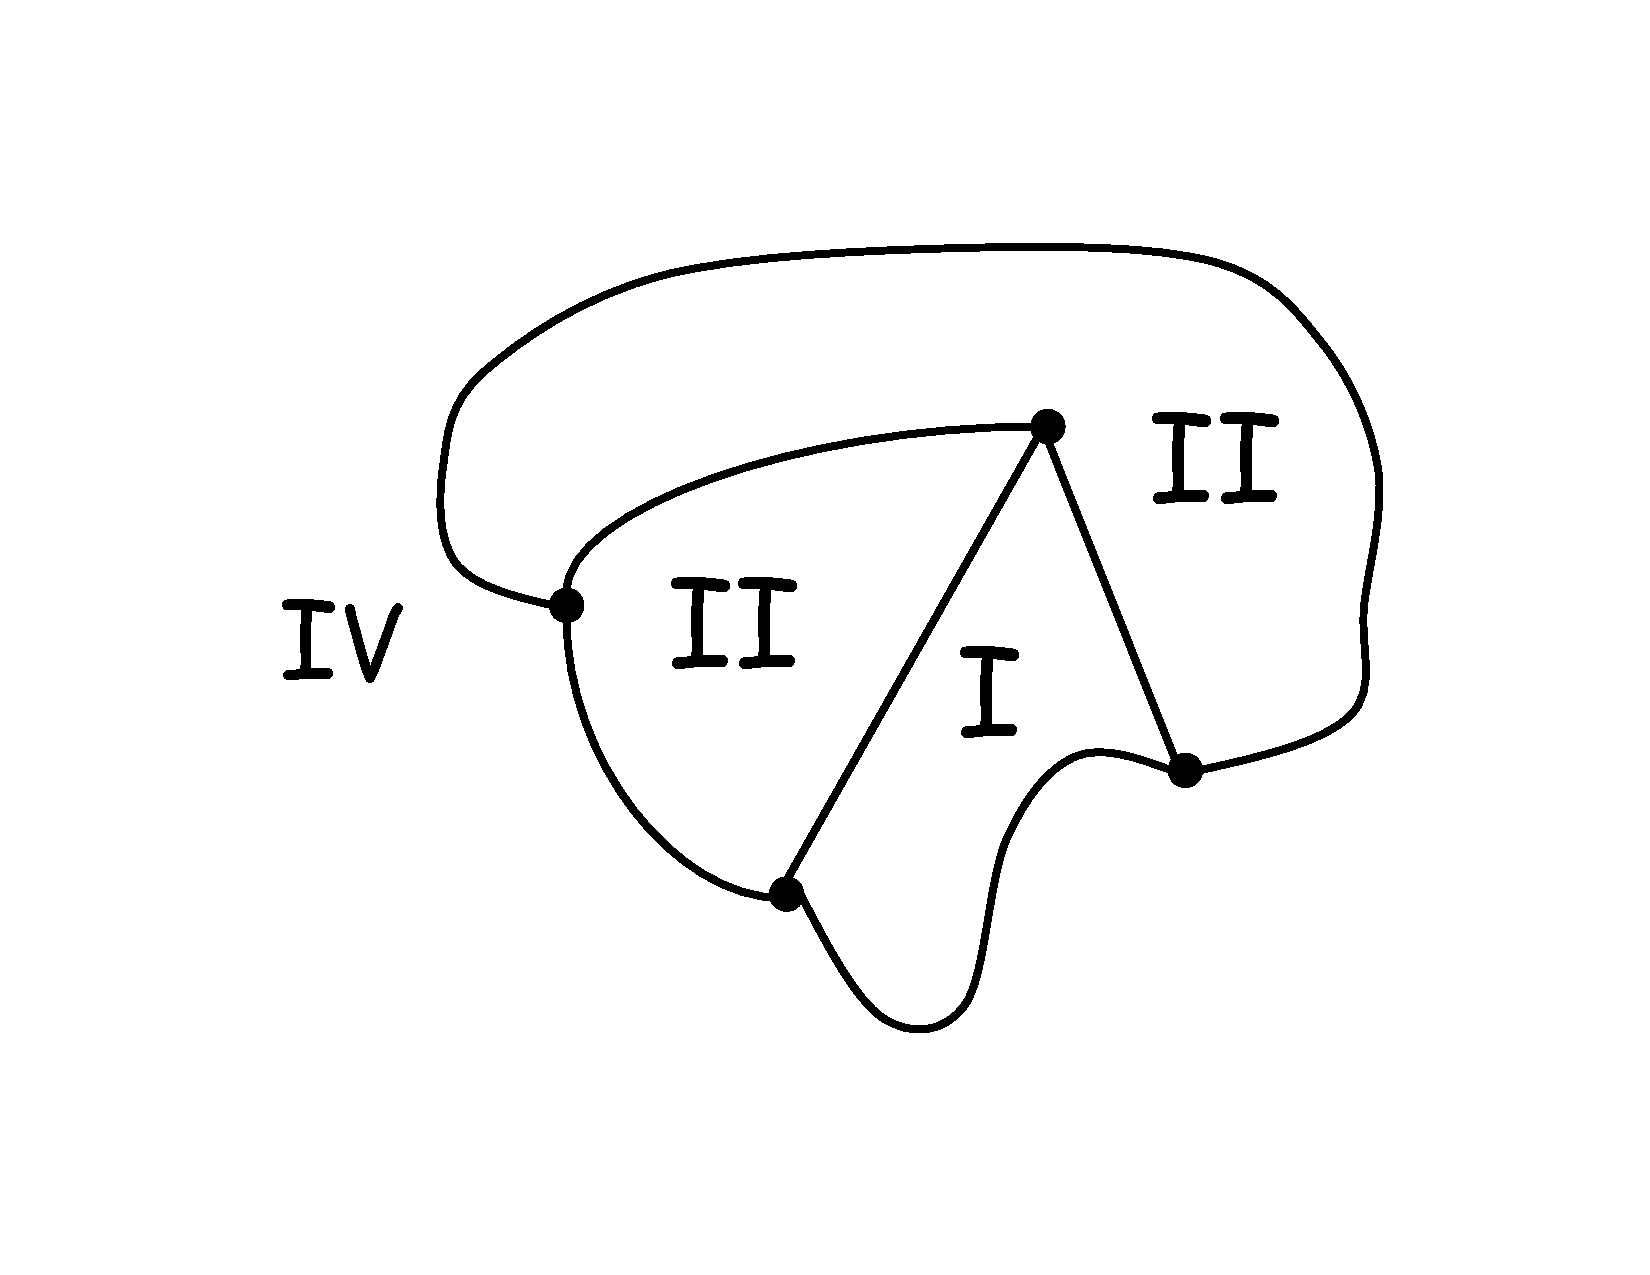
\includegraphics[height=2in]{figures/continuous-faces}
\caption{A Planar Drawing with Four Faces.}
\label{fig:continuous-faces}
\end{figure}
Face IV, which extends off to infinity in all directions, is called the
\term{outside face}.

This definition of planar graphs is perfectly precise, but completely
unsatisfying: it invokes smooth curves and continuous regions of the plane
to define a property of a discrete data type.  So the first thing we'd
like to find is a discrete data type that represents planar drawings.

The clue to how to do this is to notice that the vertices along the
boundary of each of the faces in Figure~\ref{fig:continuous-faces} form a
simple cycle.  For example, labeling the vertices as in
Figure~\ref{fig:continuous-cycles}, the simple cycles for the face
boundaries are
\[
\mathtt{abca}\qquad \mathtt{abda}\qquad \mathtt{bcdb}\qquad \mathtt{acda}.
\]
Since every edge in the drawing appears on the boundaries of exactly two
continuous faces, every edge of the simple graph appears on exactly two of
the simple cycles.

\begin{figure}
\centering 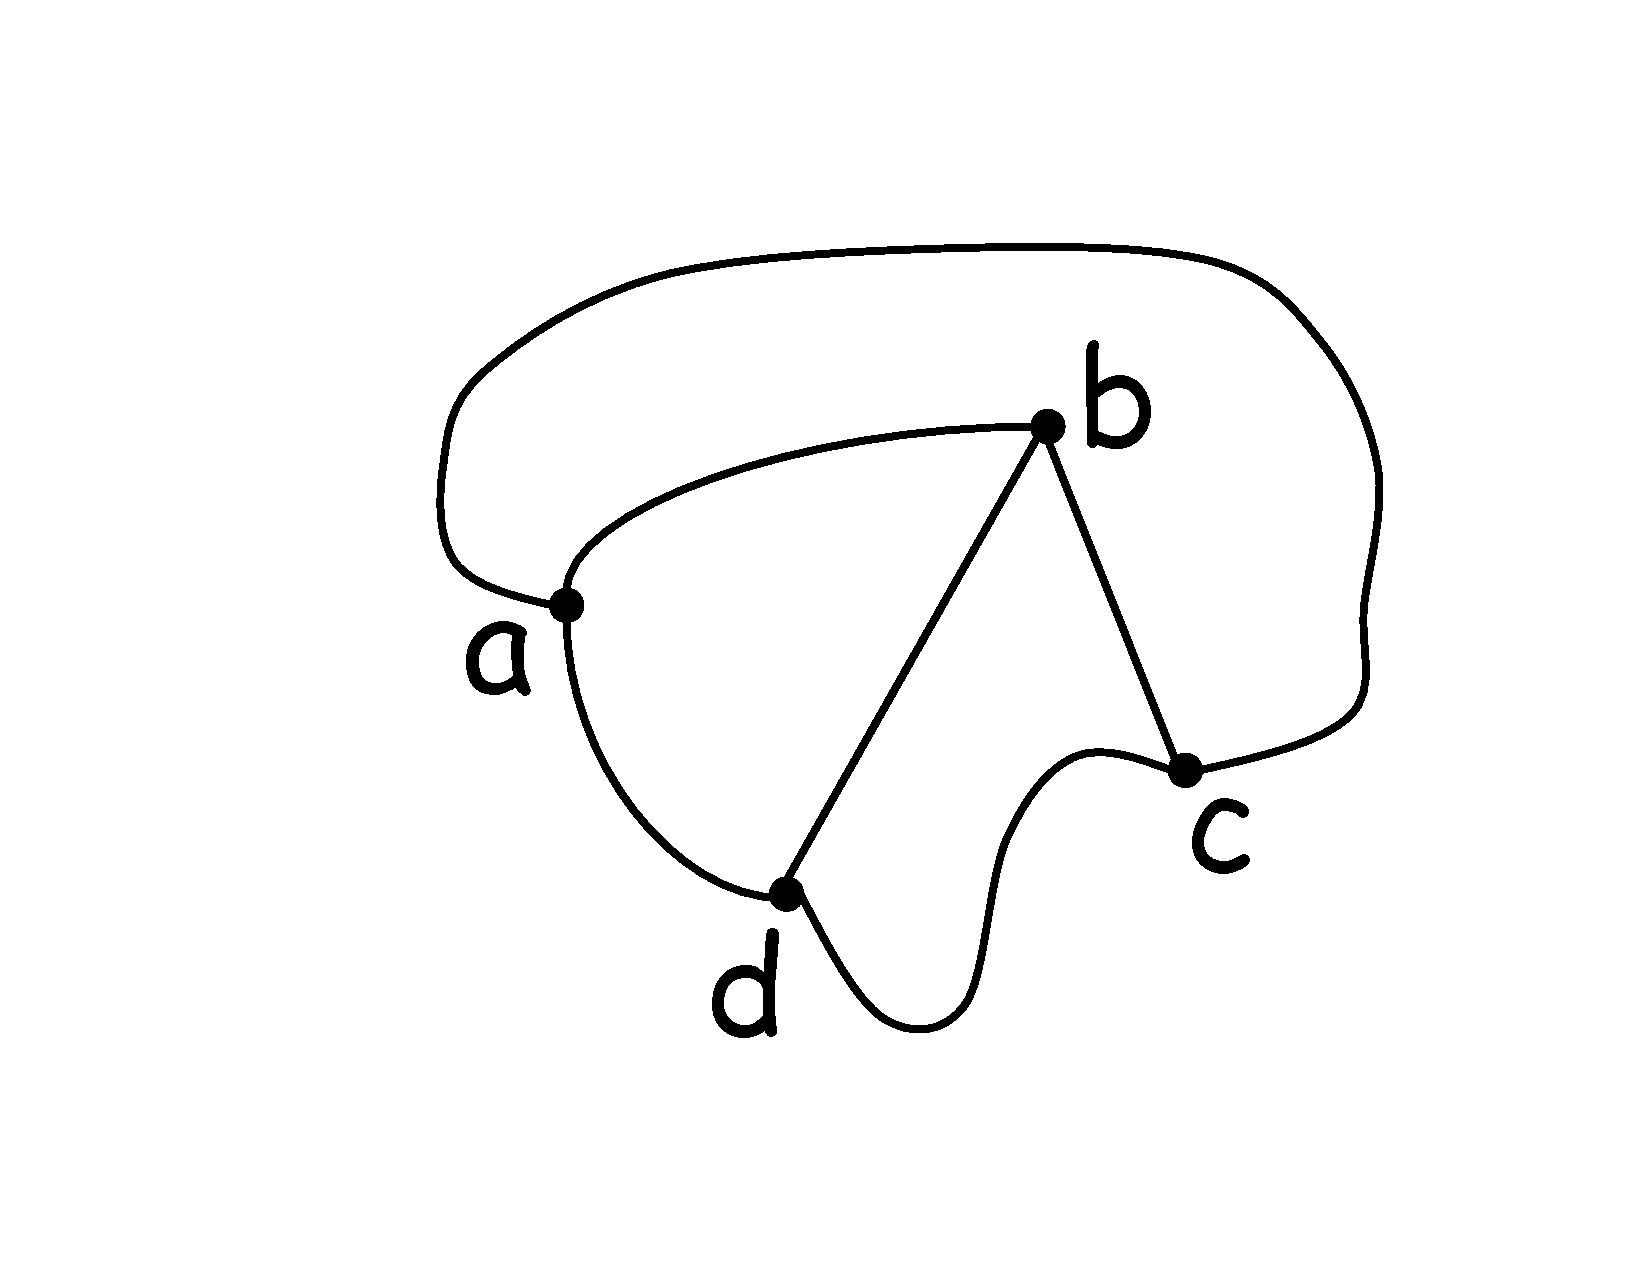
\includegraphics[height=2in]{figures/continuous-cycles}
\caption{The Drawing with Labelled Vertices.}
\label{fig:continuous-cycles}
\end{figure}

Vertices around the boundaries of states and countries in an ordinary map
are always simple cycles, but oceans are slightly messier.  The ocean
boundary is the set of all boundaries of islands and continents in the
ocean; it is a \emph{set} of simple cycles (this can happen for countries
too ---like Bangladesh).  But this happens because islands (and the two
parts of Bangladesh) are not connected to each other.  So we can dispose
of this complication by treating each connected component separately.

But general planar graphs, even when they are connected, may be a bit more
complicated than maps.  For example a planar graph may have a
``bridge,'' as in Figure~\ref{fig:bridge}.
\begin{figure}[h]
\centering 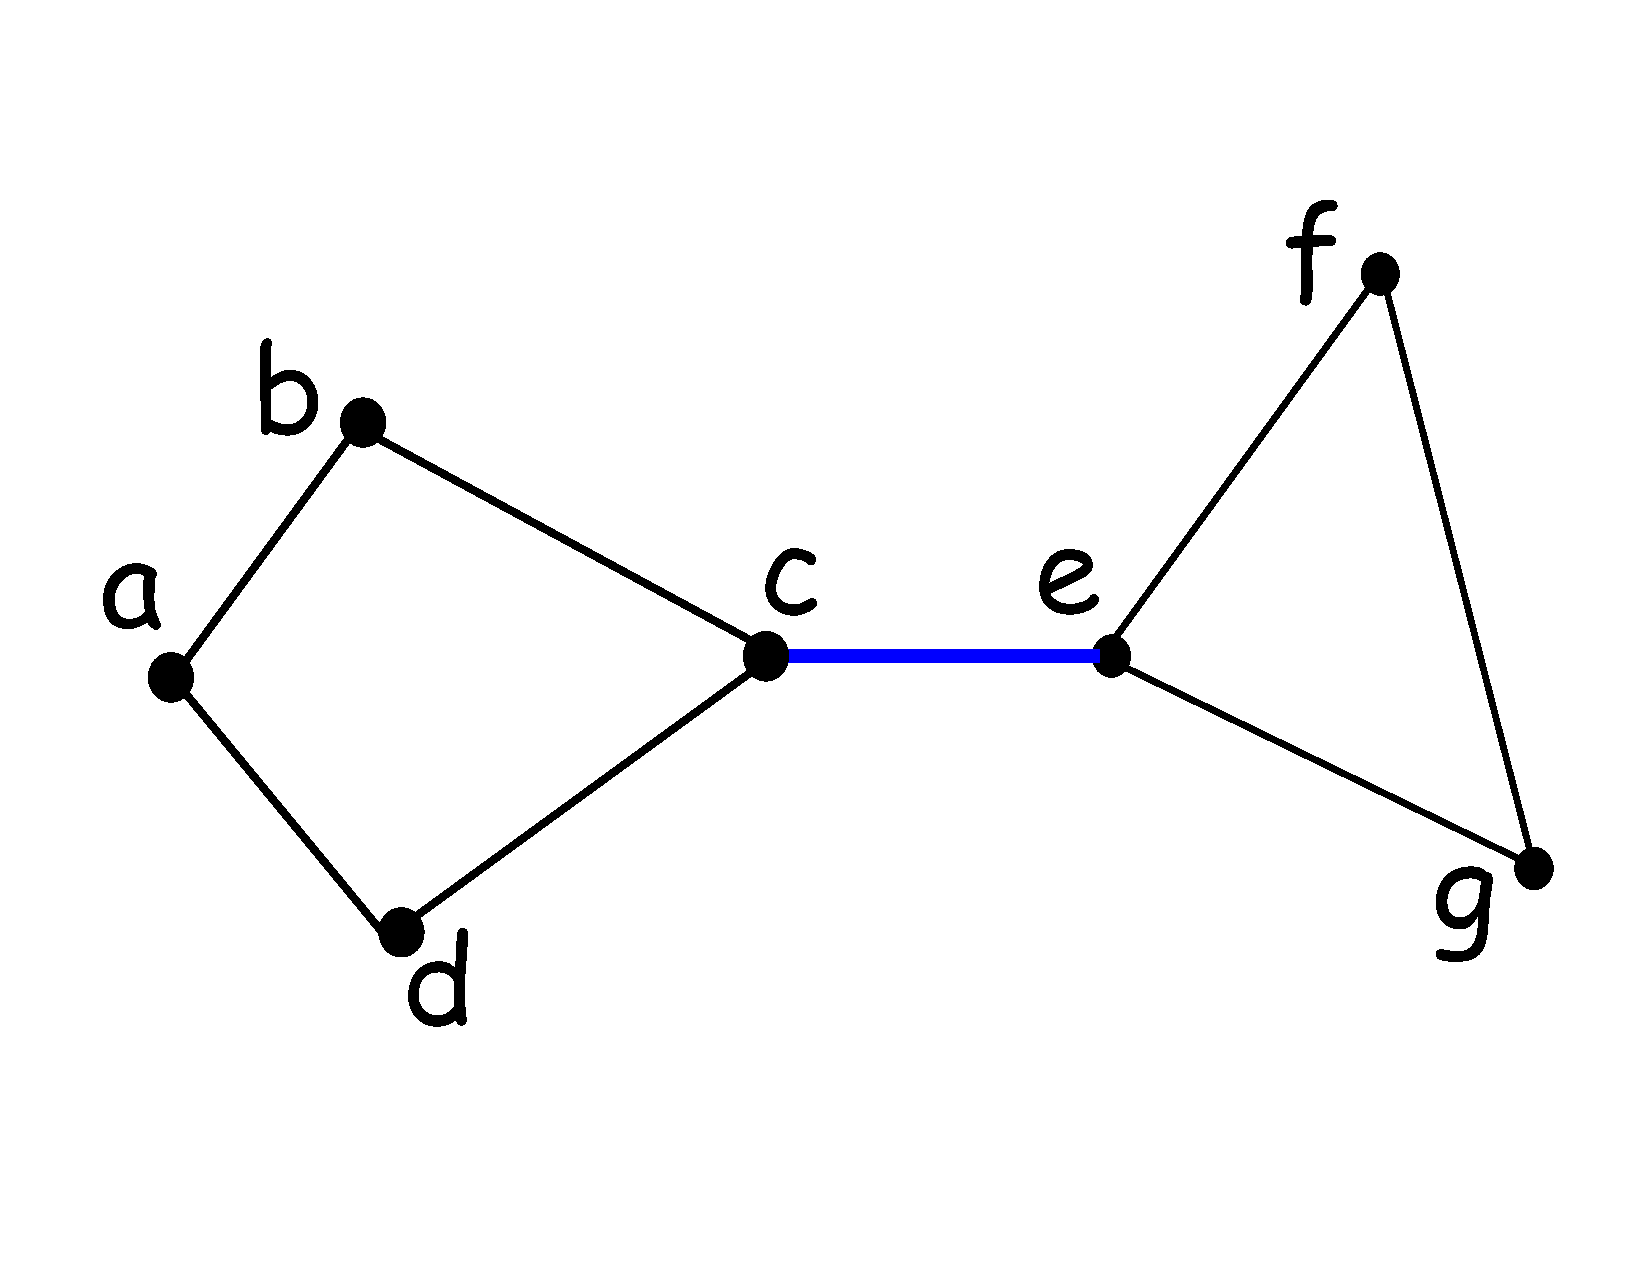
\includegraphics[height=2in]{figures/edge-twice-same-face}
\caption{A Planar Drawing with a \emph{Bridge}.}
\label{fig:bridge}
\end{figure}
Now the cycle around the outer face is
\[
\mathtt{abcefgecda}.
\]
This is not a simple cycle, since it has to traverse the bridge
$\edge{c}{e}$ twice.

Planar graphs may also have ``dongles,'' as in Figure~\ref{fig:dongle}.
\begin{figure}[h]
\centering 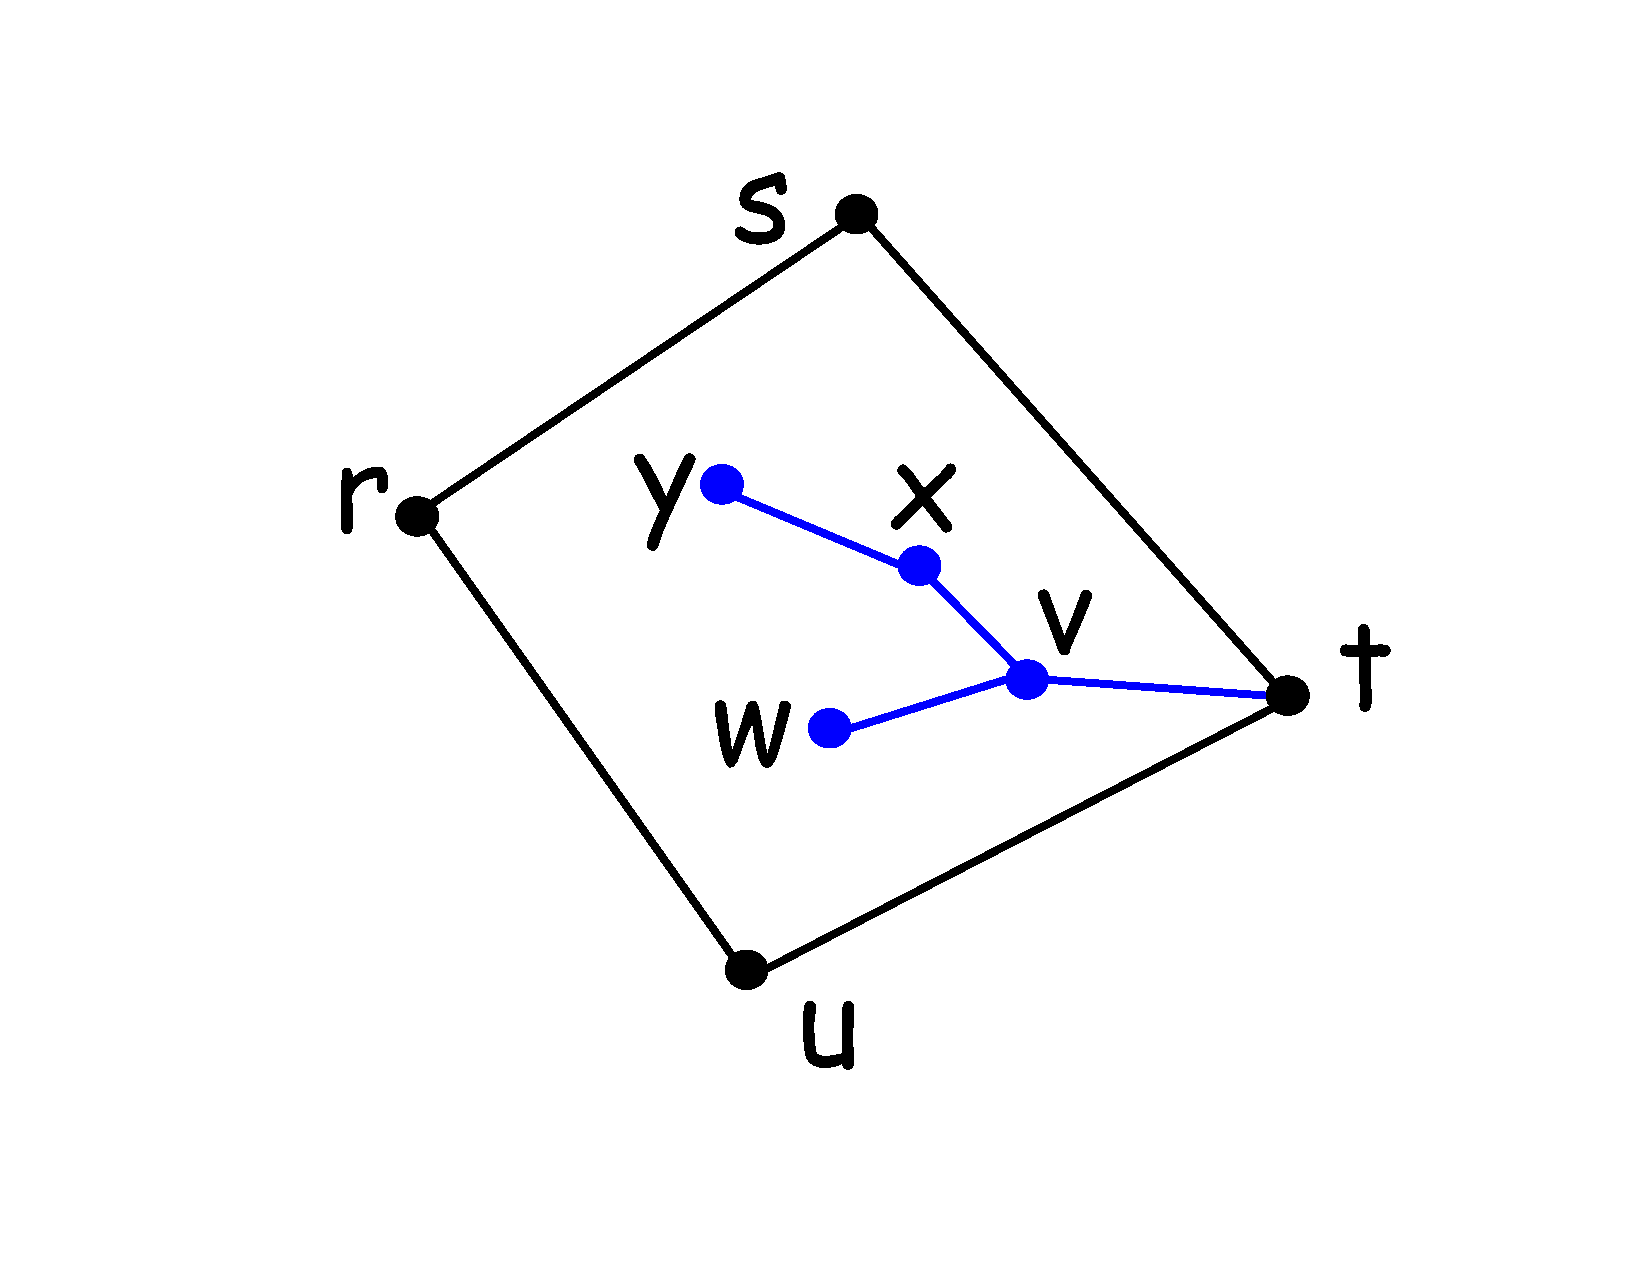
\includegraphics[height=2in]{figures/dongle-face}
\caption{A Planar Drawing with a \emph{Dongle}.}
\label{fig:dongle}
\end{figure}
Now the cycle around the inner face is
\[
\mathtt{rstvxyxvwvtur},
\]
because it has to traverse \emph{every} edge of the dongle twice ---once
``coming'' and once ``going.''

But bridges and dongles are really the only complications, which leads
us to the discrete data type of \emph{planar embeddings} that we can use
in place of continuous planar drawings.  Namely, we'll define a planar
embedding recursively to be the set of boundary-tracing cycles we could
get drawing one edge after another.

\iffalse  FAILED ATTEMPT TO AVOID RECURSIVE DEF
One property of the set of boundary-tracing cycles is that every
edge is traversed a total of two times by cycles in the set.  This is
almost enough to pin down exactly when a set of cycles are the
boundary-tracing cycles of a planar drawing, but not quite.  To illustrate
the remaining technicality, look at Figure~\ref{fig:bridge} showing a
bridge.  This graph has three faces described by the boundary-tracing
cycles
\[
\mathtt{abcefgecda} \text{ (the outer face)} \qquad \mathtt{abcda}\qquad
\mathtt{efge}.
\]
But we might also split up the cycle for the outer boundary into two
cycles, giving the set of four cycles,
\[
\mathtt{abcecda}\qquad \mathtt{efge} \qquad \mathtt{abcda}\qquad
\mathtt{efge}
\]
We don't want to allow this kind of splitting up of genuine
boundary-tracing cycles, but the four cycles above do have the property
that every edge is still traversed exactly twice.  What's wrong with the
split cycles is that they backtrack on themselves when they don't have to
---backtracks should only occur when there's nowhere else to go. More
precisely:
\begin{definition}
A cycle in a graph has a \emph{backtrack} at vertex $v$ iff it contains a
subsequence $w,v,w$ for some vertex, $w$.  A backtrack at $v$ is
\emph{necessary} iff $v$ has degree 1.
\end{definition}
Now we're finally ready to define planar embeddings.

Let $G$ be a connected graph.  A \emph{planar embedding} of $G$ is a
set\footnote{\label{C} There is one exception to this definition.  If $G$
is isomorphic to the simple cycle, $C_n$, then a planar drawing of $G$ has
an inner and an outer face with the \emph{same} simple cycle as the
boundary of both faces.  So we need to use two ``copies'' of this simple
cycle as the set of boundary cycles for this graph.  But since this is the
only situation in which two faces have the same boundary cycle, this
exception is better explained in a footnote than mentioned explicitly in
the definition.} of cycles called \emph{boundary cycles}, such that
every edge of $G$ is traversed either
\begin{itemize}
\item by exactly two boundary cycles that are simple cycles, or

\item twice by a single boundary cycle that only backtracks when
necessary.
\end{itemize}


we can eliminate having to reason about continuous faces by jumping
directly to what matters about a continuous face, namely, the sequence of
vertices on its boundary curves.  This sequence is an undirected cycle in
the graph.  We'll call such an undirected cycle a \emph{discrete face},
and refer to a graph along with its discrete faces as a \emph{planar
embedding} of the graph.

The simplest kind of discrete face comes from the boundary of a country in
a map drawing ---this would just be a simple cycle.  Also, since each edge
appears on a boundary between two countries, it is traversed a total of
two times by the set of discrete faces.

But maps of countries are only a special case of planar graph.  For
example, a tree can always be drawn in the plane.  Such a tree drawing
``divides'' the plane into just \emph{one} region whose ``boundary'' is
the points and curves in the drawing, and the cycle of successive vertices
around this boundary backtracks on itself at every leaf.  But still, every
edge in the tree is traversed exactly twice (coming and going) by the
boundary of the tree.  So a planar graph will always have a set of
discrete faces such that each edge of the graph is traversed a total of
two times by these faces.

It turns out, conversely, that if a graph has a set of discrete faces that
traverse each edge a total of two times, the graph is in fact planar.  The
idea behind this claim is to consider how the successive discrete faces
could be drawn in the plane one at a time, with each new face having all
its edges on the boundary of one of the regions created so far (and in the
right order) so it can be added without the need to cross another face.

\textbf{MORE NEEDED HERE.}

But the only way to really prove this requires working with continuous
faces and continuously connected planar regions, which we don't want to
get into.  So we'll just accept the following definition:

\begin{definition}
A \emph{planar embedding} of a graph, $G$, is a set of cycles of $G$ such
that every edge is traversed a total of two times by these cycles.  Each
cycle is called a \emph{face} of the embedding.  A graph is \emph{planar}
iff it has a planar embedding.
\end{definition}
\fi

\subsection{Planar Embeddings}

By thinking of the process of drawing a planar graph edge by edge, we can
give a useful recursive definition of planar embeddings.

\begin{definition}
A \emph{planar embedding} of a \emph{connected} graph consists of a
nonempty set of cycles of the graph called the \emph{discrete faces} of
the embedding.  Planar embeddings are defined recursively as follows:

\begin{itemize}
\item \textbf{Base case:} If $G$ is a graph consisting of a single vertex,
$v$, then a planar embedding of $G$ has one discrete face, namely the
length zero cycle, $v$.

\item \textbf{Constructor Case:} (split a face) Suppose $G$ is a
connected graph with a planar embedding, and suppose $a$ and $b$ are
distinct, nonadjacent vertices of $G$ that appear on some discrete face,
$\gamma$, of the planar embedding.  That is, $\gamma$ is a cycle of the form
\[
a \dots b \cdots a.
\]
Then the graph obtained by adding the edge $\edge{a}{b}$ to the edges of
$G$ has a planar embedding with the same discrete faces as $G$, except
that face $\gamma$ is replaced by the two discrete
faces\footnote{\label{C} There is one exception to this rule.  If $G$ is a
line graph beginning with $a$ and ending with $b$, then the cycles into
which $\gamma$ splits are actually the same.  That's because adding edge
$\edge{a}{b}$ creates a simple cycle graph, $C_n$, that divides the plane
into an ``inner'' and an ``outer'' region with the same border.  In order
to maintain the correspondence between continuous faces and discrete
faces, we have to allow two ``copies'' of this same cycle to count as
discrete faces.  But since this is the only situation in which two faces
are actually the same cycle, this exception is better explained in a
footnote than mentioned explicitly in the definition.}
\[
a\dots ba\quad \text{ and } \quad ab\cdots a, 
\]
as illustrated in Figure~\ref{fig:face-splitting}.

\begin{figure}[h]
\centering 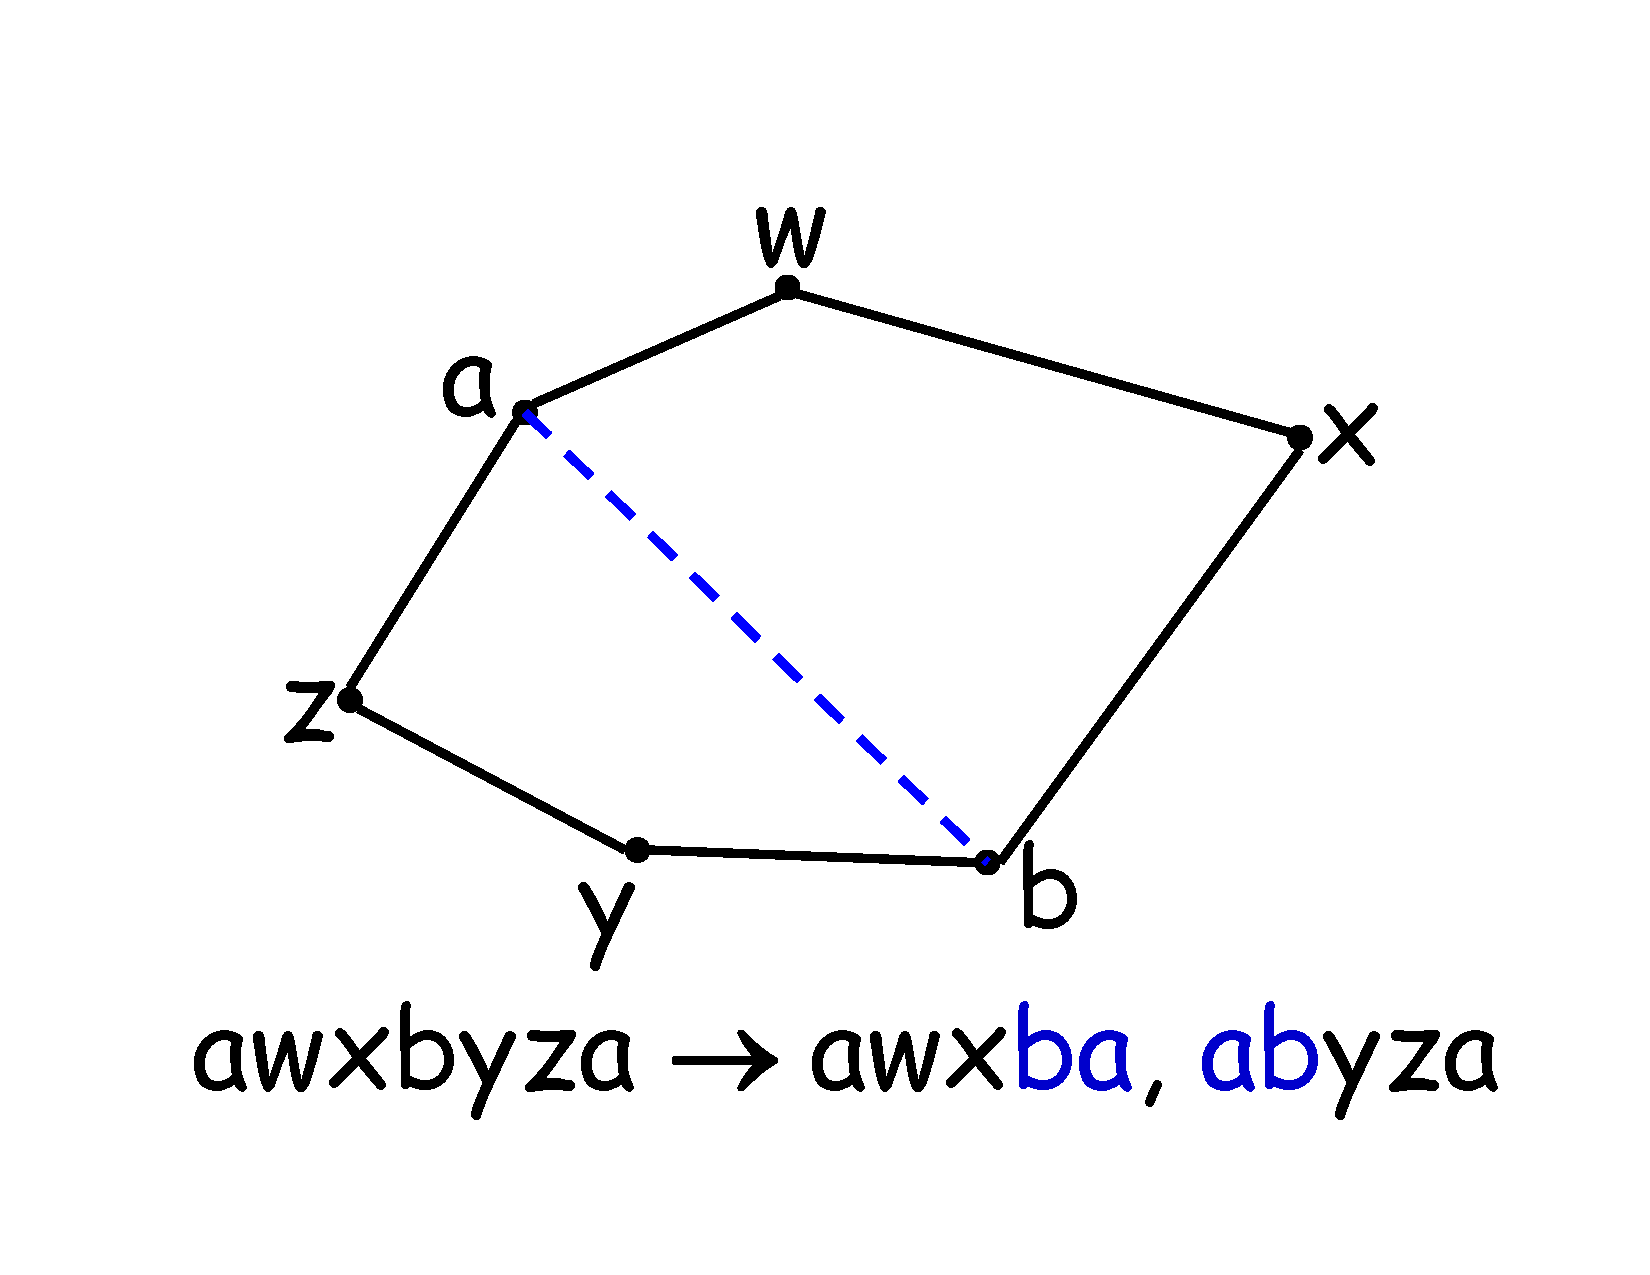
\includegraphics[height=2.5in]{figures/split-a-face}
\caption{The Split a Face Case.}
\label{fig:face-splitting}
\end{figure}

\item \textbf{Constructor Case:} (add a bridge) Suppose $G$ and $H$ are
connected graphs with planar embeddings and disjoint sets of vertices.
Let $a$ be a vertex on a discrete face, $\gamma$, in the embedding of
$G$.  That is, $\gamma$ is of the form
\[
a\dots a.
\]
Similarly, let $b$ be a vertex on a discrete face, $\delta$, in the
embedding of $H$, so $\delta$ is of the form
\[
b\cdots b.
\]
Then the graph obtained by connecting $G$ and $H$ with a new edge,
$\edge{a}{b}$, has a planar embedding whose discrete faces are the union of
the discrete faces of $G$ and $H$, except that faces $\gamma$ and $\delta$
are replaced by one new face
\[
a\dots ab\cdots ba.
\]
This is illustrated in Figure~\ref{fig:add-bridge}, where the faces of
$G$ and $H$ are:
\[
G: \set{\texttt{axyza},\ \texttt{axya},\ \texttt{ayza}}
    \qquad H: \set{\texttt{btuvwb},\ \texttt{btvwb},\ \texttt{tuvt}},
\]
and after adding the bridge $\edge{\texttt{a}}{\texttt{b}}$, there is a
single connected graph with faces
\[
\set{\texttt{axyz{\color{blue}ab}tuvw{\color{blue}ba}},\ 
         \texttt{axya},\ \texttt{ayza},\ \texttt{btvwb},\ \texttt{tuvt}}.
\]
\begin{figure}[h]
\centering 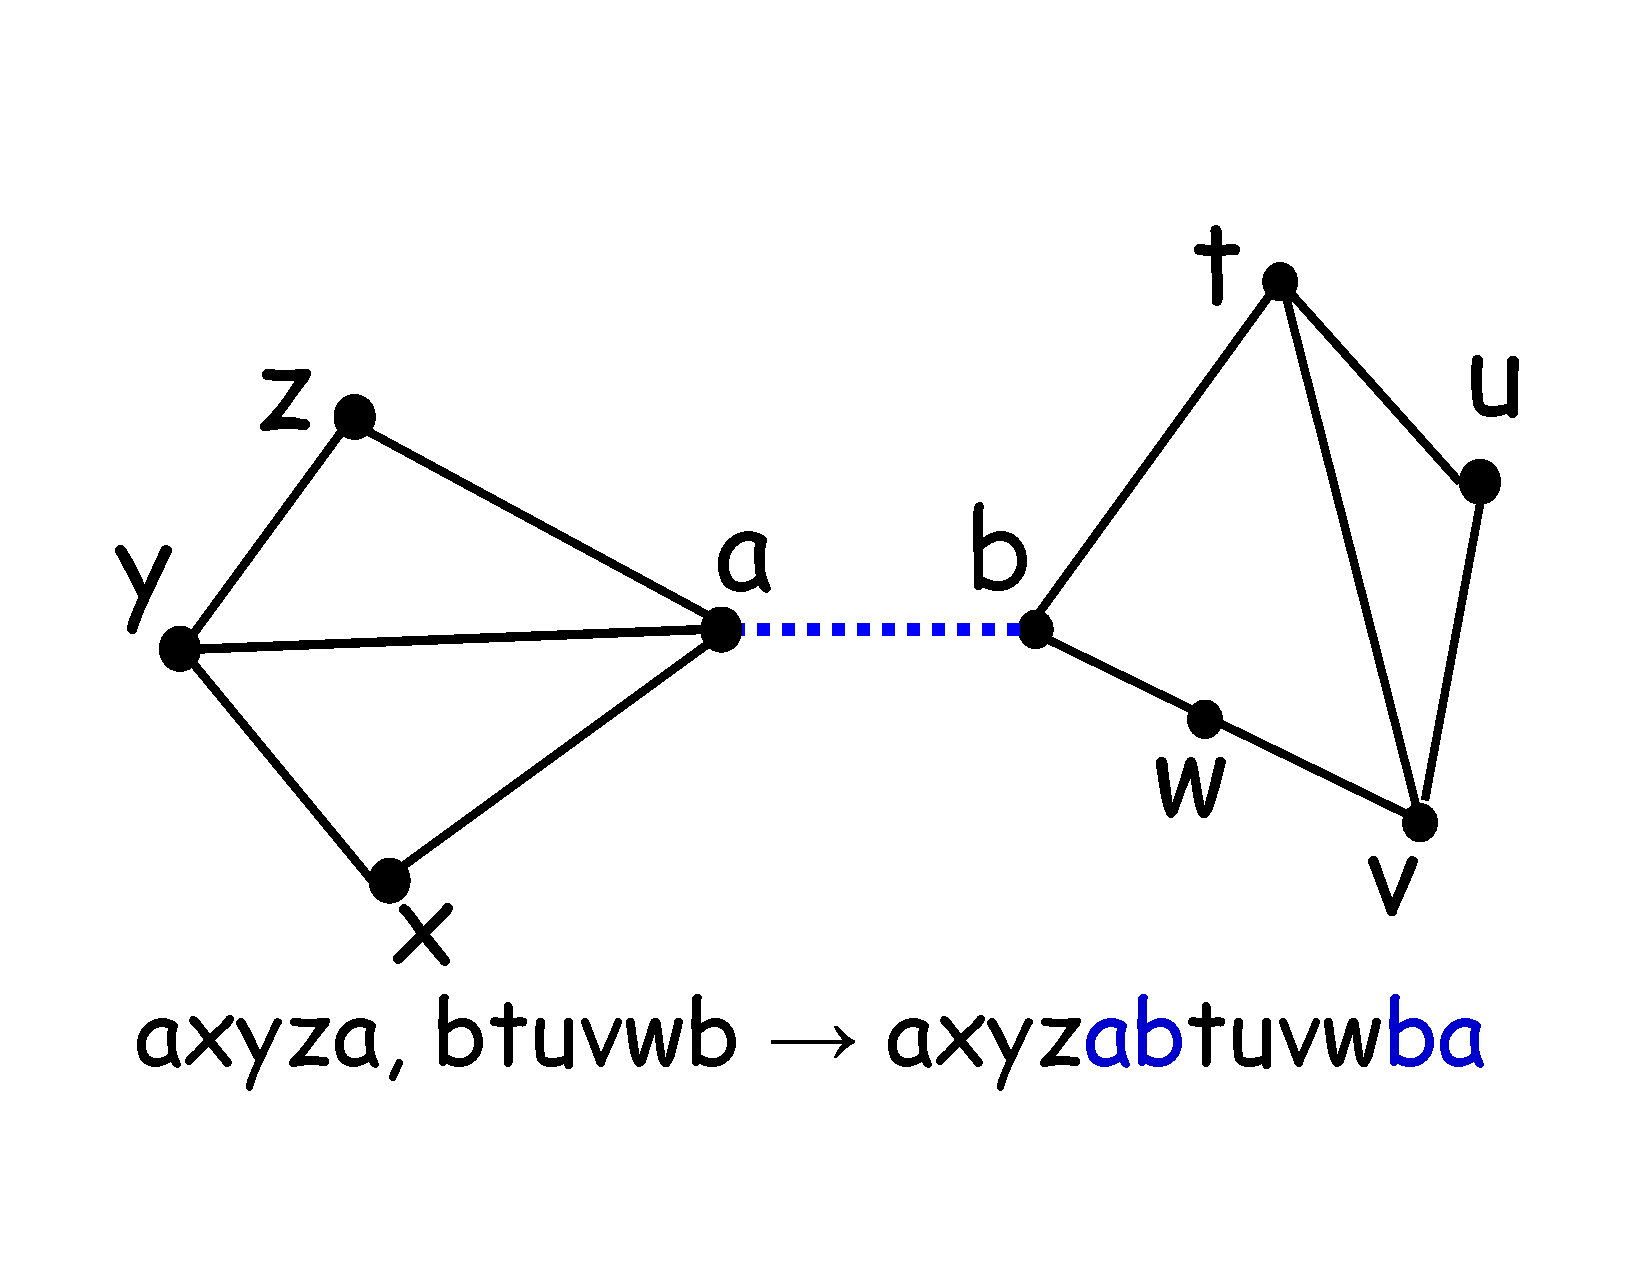
\includegraphics[height=3in]{figures/add-bridge}
\caption{The Add Bridge Case.}
\label{fig:add-bridge}
\end{figure}

\end{itemize}

An arbitrary graph is \emph{planar} iff each of its connected components
has a planar embedding.

\end{definition}

\subsection{What outer face?}
Notice that the definition of planar embedding does not distinguish an
``outer'' face.  There really isn't any need to distinguish one.

In fact, a planar embedding could be drawn with any given face on the
outside.  An intuitive explanation of this is to think of drawing the
embedding on a \emph{sphere} instead of the plane.  Then any face can be
made the outside face by ``puncturing'' that face of the sphere,
stretching the puncture hole to a circle around the rest of the faces,
and flattening the circular drawing onto the plane.

So pictures that show different ``outside'' boundaries may actually be
illustrations of the same planar embedding.

This is what justifies the ``add bridge'' case in a planar embedding:
whatever face is chosen in the embeddings of each of the disjoint planar
graphs, we can draw a bridge between them without needing to cross any
other edges in the drawing, because we can assume the bridge connects
two ``outer'' faces.

\subsection{Euler's Formula}

The value of the recursive definition is that it provides a powerful
technique for proving properties of planar graphs, namely, structural
induction.

One of the most basic properties of a connected planar graph is that its
number of vertices and edges determines the number of faces in every
possible planar embedding:

\begin{theorem}[Euler's Formula]
If a connected graph has a planar embedding, then
%
\[
v - e + f = 2
\]
%
where $v$ is the number of vertices, $e$ is the number of edges, and
$f$ is the number of faces.
\end{theorem}

For example, in Figure~\ref{fig:continuous-faces}, $\card{V} = 4$,
$\card{E} = 6$, and $f = 4$.  Sure enough, $4 - 6 + 4 = 2$, as Euler's
Formula claims.


\begin{proof}
The proof is by structural induction on the definition of planar
embeddings.  Let $P(\embed{E})$ be the proposition that $v - e + f = 2$ for an
embedding, $\embed{E}$.

\textbf{Base case:} ($\embed{E}$ is the one vertex planar embedding).
By definition, $v=1$, $e=0$, and $f=1$, so $P(\embed{E})$ indeed holds.

\textbf{Constructor case:} (split a face) Suppose $G$ is a connected graph
with a planar embedding, and suppose $a$ and $b$ are distinct, nonadjacent
vertices of $G$ that appear on some discrete face,
$\gamma= a \dots b \cdots a$, of the planar embedding.

Then the graph obtained by adding the edge $\edge{a}{b}$ to the edges of
$G$ has a planar embedding with one more face and one more edge than $G$.
So the quantity $v-e+f$ will remain the same for both graphs, and since by
structural induction this quantity is 2 for $G$'s embedding, it's also 2
for the embedding of $G$ with the added edge.  So $P$ holds for the
constructed embedding.

\textbf{Constructor case:} (add bridge) Suppose $G$ and $H$ are connected
graphs with planar embeddings and disjoint sets of vertices.  Then
connecting these two graphs with a bridge merges the two bridged faces
into a single face, and leaves all other faces unchanged.  So the bridge
operation yields a planar embedding of a connected graph with $v_G +v_H$
vertices, $e_G + e_H +1$ edges, and $f_G + f_H - 1$ faces.  But
\begin{align*}
\lefteqn{(v_G +v_H) - (e_G + e_H +1) + (f_G + f_H - 1)}\\
   & = (v_G  - e_G + f_G) + (v_H  - e_H  + f_H) -2\\
   & = (2)+(2)-2 & \text{(by structural induction hypothesis)}\\
   & = 2.
\end{align*}
So $v-e+f$ remains equal to 2 for the constructed embedding.  That is, $P$
also holds in this case.

This completes the proof of the constructor cases, and the theorem follows
by structural induction.
\end{proof}

\iffalse
\mfigure{!}{1in}{figures/planar-assumptions.pdf}
\fi

\subsection{Number of Edges versus Vertices}

Like Euler's formula, the following lemmas follow by structural induction
directly from the definition of planar embedding.

\begin{lemma}\label{2e}
In a planar embedding of a connected graph, each edge is traversed once by
each of two different faces, or is traversed exactly twice by one face.
\end{lemma}

\begin{lemma}\label{3f}
  In a planar embedding of a connected graph with at least three vertices,
  each face is of length at least three.
\end{lemma}

\begin{corollary}
\label{e3v}
Suppose a connected planar graph has $v \geq 3$ vertices and $e$ edges.
Then
\[
e \leq 3v-6.
\]
\end{corollary}

\begin{proof}
By definition, a connected graph is planar iff it has a planar embedding.
So suppose a connected graph with $v$ vertices and $e$ edges has a planar
embedding with $f$ faces.  By Lemma~\ref{2e}, every edge is traversed
exactly twice by the face boundaries.  So the sum of the lengths of the
face boundaries is exactly $2e$.  Also by Lemma~\ref{3f}, when $v \geq 3$,
each face boundary is of length at least three, so this sum is at least
$3f$.  This implies that
\begin{equation}\label{e3f}
3f \leq 2e.
\end{equation}
But $f = e-v+2$ by Euler's formula, and substituting into~\eqref{e3f} gives
\begin{align*}
3(e-v+2) & \leq 2e\\
e-3v + 6  & \leq 0\\
e & \leq 3v - 6
\end{align*}
\end{proof}

Corollary~\ref{e3v} lets us prove that the quadapi can't all shake hands
without crossing.  Representing quadapi by vertices and the necessary
handshakes by edges, we get the complete graph, $K_5$.  Shaking hands
without crossing amounts to showing that $K_5$ is planar.  But $K_5$ is
connected, has 5 vertices and 10 edges, and $10 > 3 \cdot 5-6$.  This
violates the condition of Corollary~\ref{e3v} required for $K_5$ to be
planar, which proves

\begin{lemma}\label{k5not}
$K_5$ is not planar.
\end{lemma}

Another consequence is
\begin{lemma}\label{d5}
Every planar graph has a vertex of degree at most five.
\end{lemma}

\begin{proof}
If every vertex had degree at least 6, then the sum of the
vertex degrees is at least $6v$, but since the sum equals $2e$, we have
$e \geq 3v$ contradicting the fact that $e \leq 3v-6 < 3v$ by Corollary~\ref{e3v}.
\end{proof}

\begin{notesproblem}\label{e2v}
\bparts

\ppart
Show that if a connected planar graph with more than two vertices is
bipartite, then
\begin{equation}\label{2v}
e \leq 2v -4.
\end{equation}
\hint The proof of Lemma~\ref{k5not}.

\solution{By Lemma~\ref{3f}, every face is of length at least 3.  But all
  cycles in a bipartite graph are of even length, and so every face of an
  embedding must be of length at least 4.

Each edge is traversed by exactly two faces, so
\begin{equation}\label{4f}
2e = \sum_{f \in\text{ faces}} \text{length}(f) \geq \sum_{f
  \in\text{ faces}} 4 = 4f.
\end{equation}
By Euler's formula, $f = e-v+2$, so
substituting for $f$ in~\eqref{4f}, yields
\[
2e \geq 4(e-v+2),
\]
which simplifies to~\eqref{2v}.
}

\ppart\label{k33not} Conclude that $K_{3,3}$ is not planar.

\solution{$K_{3,3}$ is bipartite and connected. Also, it has 9 edges and 6
  vertices, and since $9 > 8 = 2 \cdot 6 - 4$, it does not
  satisfy~\eqref{2v}, and so cannot be planar.}

\eparts
\end{notesproblem}

\subsection{Planar Subgraphs}

If you draw a graph in the plane by repeatedly adding edges that don't
cross, you clearly could add the edges in any other order and still wind
up with the same drawing.  This is so basic that we might presume that our
recursively defined planar embeddings have this property.  But that
wouldn't be fair: we really need to prove it.  After all, the recursive
definition of planar embedding was pretty technical ---maybe we got it a
little bit wrong, with the result that our embeddings don't have this basic
draw-in-any-order property.

Now any ordering of edges can be obtained just by repeatedly switching the
order of successive edges, and if you think about the recursive definition
of embedding for a minute, you should realize that you can switch
\emph{any} pair of successive edges if you can just switch the last two.
So it all comes down to the following lemma.

\hyperdef{switch}{edges}{\begin{lemma}}\label{switch-edges} Suppose that,
  starting from some embeddings of planar graphs with disjoint sets of
  vertices, it is possible by two successive applications of constructor
  operations to add edges $e$ and then $f$ to obtain a planar embedding,
  $\embed{F}$.  Then starting from the same embeddings, it is also
  possible to obtain $\embed{F}$ by adding $f$ and then $e$ with two
  successive applications of constructor operations.
\end{lemma}

\begin{corollary}\label{permute-edges} Suppose that, starting from some
  embeddings of planar graphs with disjoint sets of vertices, it is
  possible to add a sequence of edges $e_0,e_1,\dots,e_n$ by successive
  applications of constructor operations to obtain a planar embedding,
  $\embed{F}$.  Then starting from the same embeddings, it is also
  possible to obtain $\embed{F}$ by applications of constructor operations
  that successively add any permutation\footnote{If $\pi:\set{0,1,\dots,n} \to
    \set{0,1,\dots,n}$ is a bijection, then the sequence
    $e_{\pi(0)},e_{\pi(1)},\dots,e_{\pi(n)}$ is called a \term{permutation} of
    the sequence $e_0,e_1,\dots,e_n$.} of the edges $e_0,e_1,\dots,e_n$.
\end{corollary}

\begin{notesproblem}{}
\bparts

\ppart  Prove Lemma~\ref{switch-edges}.  \hint There are four cases to analyze,
  depending on which two constructor operations are applied to add $e$ and
  then $f$.  Structural induction is not needed.

\ppart Prove Corollary~\ref{permute-edges}.

\hint By induction on the number of switches of adjacent elements needed
to convert the sequence 0,1,\dots,$n$ into a permutation
$\pi(0),\pi(1),\dots,\pi(n)$.

\eparts
\end{notesproblem}

\begin{corollary}\label{delete-edge}
Deleting an edge from a planar graph leaves a planar graph.

\begin{proof}
  By Corollary~\ref{permute-edges}, we may assume the deleted edge was the
  last one added in constructing an embedding of the graph.  So the
  embedding to which this last edge was added must be an embedding of the
  graph without that edge.
\end{proof}

\end{corollary}

Since we can delete a vertex by deleting all its incident edges,
Corollary~\ref{delete-edge} immediately implies

\begin{corollary}\label{delete-vertex}
Deleting a vertex from a planar graph, along with all its incident
edges of course, leaves another planar graph.
\end{corollary}

A \emph{subgraph} of a graph, $G$, is any graph whose set of vertices is a
subset of the vertices of $G$ and whose set of edges is a subset of the
set of edges of $G$.  So we can summarize Corollaries~\ref{delete-edge}
and~\ref{delete-vertex} and their consequences in a Theorem.

\begin{theorem}\label{planar-subgraph}
  Any subgraph of a planar graph is planar.
\end{theorem}

\subsection{Planar 5-Colorability}

We need to know one more property of planar graphs in order to prove that
planar graphs are 5-colorable.

\begin{lemma}\label{mergelem}
Merging two adjacent vertices of a planar graph leaves another planar graph.
\end{lemma}

Here merging two adjacent vertices, $n_1$ and $n_2$ of a graph means
deleting the two vertices and then replacing them by a new ``merged''
vertex, $m$, adjacent to all the vertices that were adjacent to either of
$n_1$ or $n_2$, as illustrated in Figure~\ref{fig:merged}.

\begin{figure}[h]
\centering 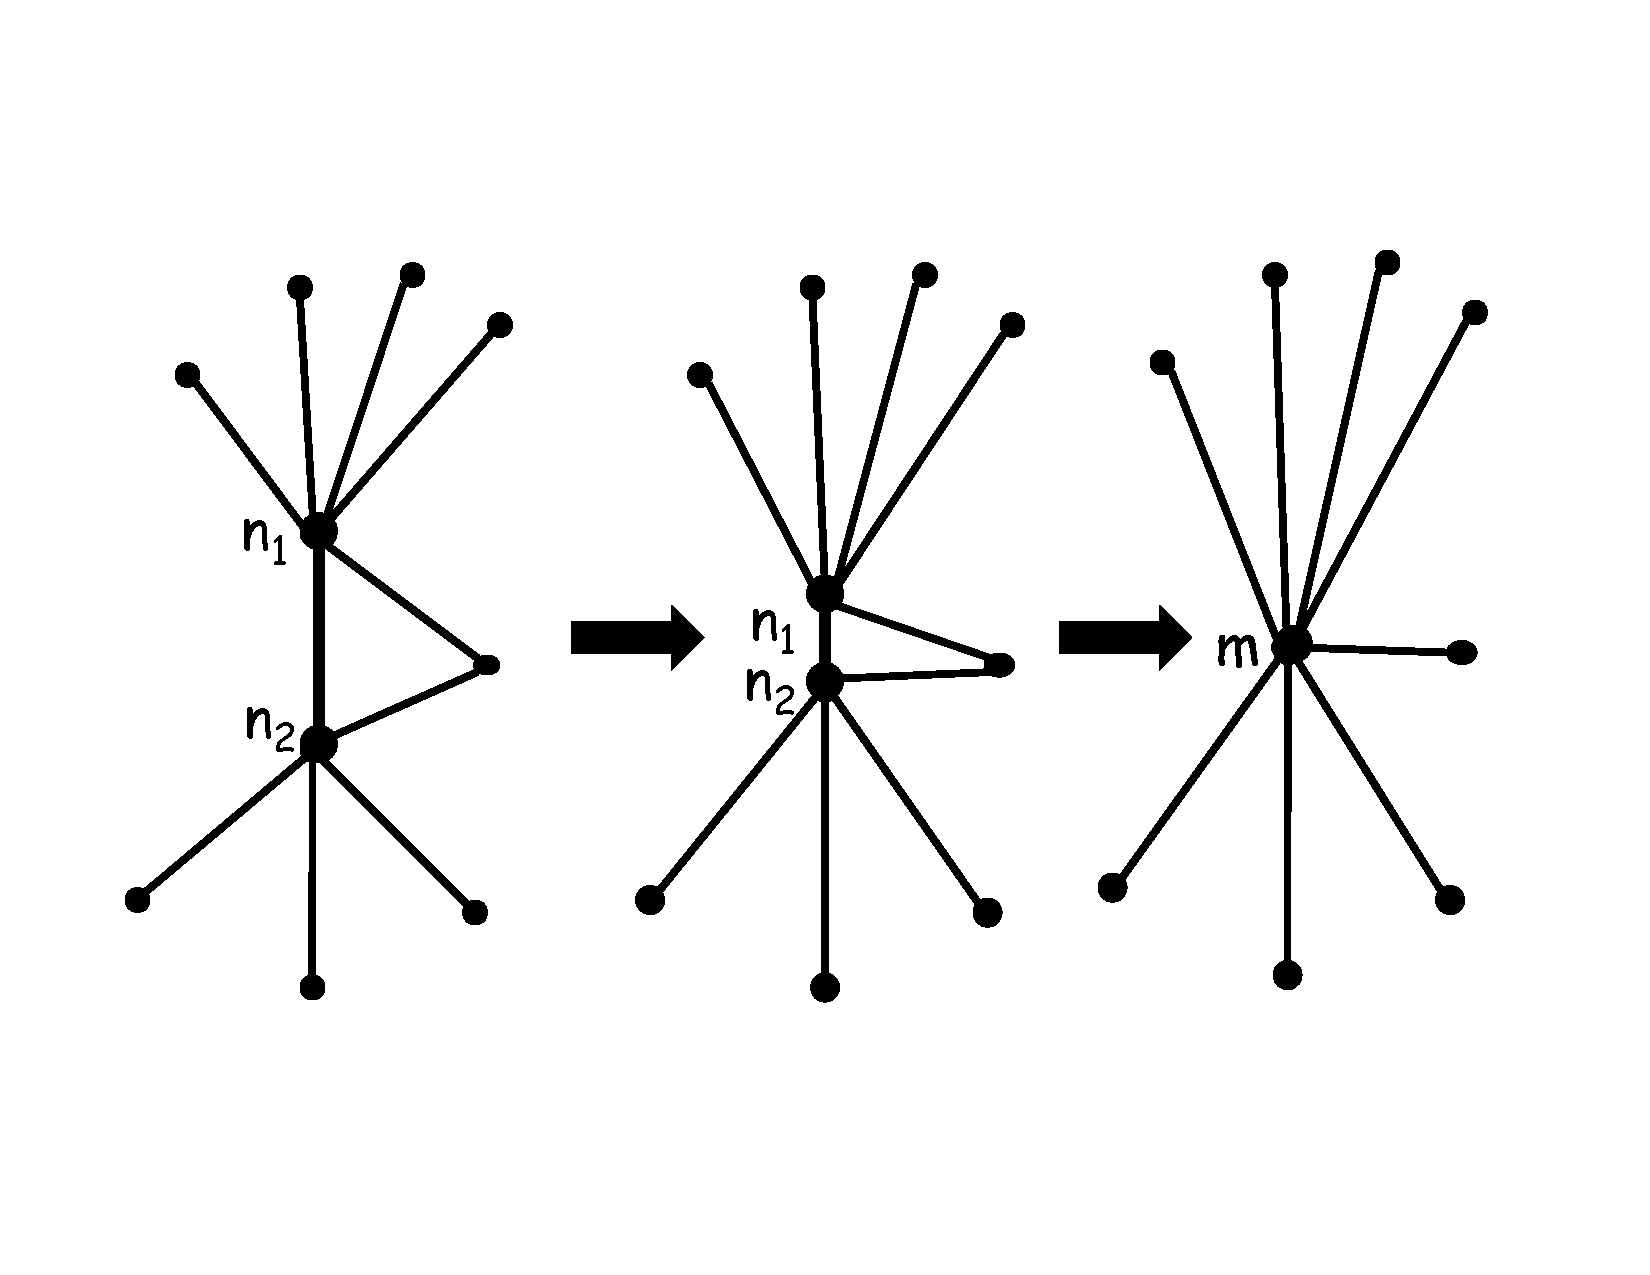
\includegraphics[height=5in]{figures/vertex-merge-arrows.pdf}
\caption{Merging adjacent vertices $n_1$ and $n_2$ into new vertex, $m$.}
\label{fig:merged}
\end{figure}

Lemma~\ref{mergelem} can be proved by structural induction, but the proof
is kind of boring, and we hope you'll be relieved that we're going to omit
it.  (If you insist, we can add it to the next problem set.)

Now we've got all the simple facts we need to prove 5-colorability.
\begin{theorem}
Every planar graph is five-colorable.
\end{theorem}

\begin{proof}
The proof will be by strong induction on the number, $v$, of vertices, with
induction hypothesis:
\begin{quote}
Every planar graph with $v$ vertices is five-colorable.
\end{quote}

\textbf{Base cases} ($v \leq 5$): immediate.

\textbf{Inductive case}: Suppose $G$ is a planar graph with $v+1$
vertices.  We will describe a five-coloring of $G$.

First, choose a vertex, $g$, of $G$ with degree at most 5; Lemma~\ref{d5}
guarantees there will be such a vertex.

\textbf{Case 1} ($\degr{g}<5$): Deleting $g$ from $G$ leaves a graph, $H$,
that is planar by Lemma~\ref{delete-vertex}, and, since $H$ has $v$ vertices,
it is five-colorable by induction hypothesis.  Now define a five coloring
of $G$ as follows: use the five-coloring of $H$ for all the vertices besides
$g$, and assign one of the five colors to $g$ that is not the same as the
color assigned to any of its neighbors.  Since there are fewer than 5
neighbors, there will always be such a color available for $g$.

\textbf{Case 2} ($\degr{g}=5$): If the five neighbors of $g$ in $G$ were
all adjacent to each other, then these five vertices would form a
nonplanar subgraph isomorphic to $K_5$, contradicting
Theorem~\ref{planar-subgraph}.  So there must be two neighbors, $n_1$ and
$n_2$, of $g$ that are not adjacent.  Now merge $n_1$ and $g$ into a new
vertex, $m$, as in Figure~\ref{fig:merged}.  In this new graph, $n_2$ is
adjacent to $m$, and the graph is planar by Lemma~\ref{mergelem}.  So we
can then merge $m$ and $n_2$ into a another new vertex, $m'$, resulting in
a new graph, $G'$, which by Lemma~\ref{mergelem} is also planar.  Now $G'$
has $v-1$ vertices and so is five-colorable by the induction hypothesis.

Now define a five coloring of $G$ as follows: use the five-coloring of $G'$
for all the vertices besides $g$, $n_1$ and $n_2$.  Next assign the color
of $m'$ in $G'$ to be the color of the neighbors $n_1$ and $n_2$.  Since
$n_1$ and $n_2$ are not adjacent in $G$, this defines a proper
five-coloring of $G$ except for vertex $g$.  But since these two neighbors
of $g$ have the same color, the neighbors of $g$ have been colored using
fewer than five colors altogether.  So complete the five-coloring of $G$ by
assigning one of the five colors to $g$ that is not the same as any of the
colors assigned to its neighbors.

\end{proof}

A graph obtained from a graph, $G$, be repeatedly deleting vertices,
deleting edges, and merging adjacent vertices is called a \term{minor} of
$G$.  Since $K_5$ and $K_{3,3}$ are not planar,
Lemmas~\ref{delete-edge},~\ref{delete-vertex}, and~\ref{mergelem}
immediately imply:

\begin{corollary}\label{forbiddenK}
  A graph which has $K_5$ or $K_{3,3}$ as a minor is not planar.
\end{corollary}

We don't have time to prove it, but the converse of
Corollary~\ref{forbiddenK} is also true.  This gives the following famous,
very elegant, and purely discrete characterization of planar graphs:

\begin{theorem}[Kuratowksi]
  A graph is not planar iff it has $K_5$ or $K_{3,3}$ as a minor.
\end{theorem}

\subsection{Classifying Polyhedra}

The Pythagoreans had two great mathematical secrets, the irrationality of
$\sqrt{2}$ and a geometric construct that we're about to rediscover!

A \term{polyhedron} is a convex, three-dimensional region bounded by a
finite number of polygonal faces.  If the faces are identical regular
polygons and an equal number of polygons meet at each corner, then the
polyhedron is \term{regular}.  Three examples of regular polyhedra are
shown below: the tetrahedron, the cube, and the octahedron.

%\mfigure{!}{1.25in}{figures/polyhedra.pdf}
\begin{center}
\setlength{\unitlength}{3000sp}%{3947sp}%
%
\begingroup\makeatletter\ifx\SetFigFont\undefined%
\gdef\SetFigFont#1#2#3#4#5{%
  \reset@font\fontsize{#1}{#2pt}%
  \fontfamily{#3}\fontseries{#4}\fontshape{#5}%
  \selectfont}%
\fi\endgroup%
\begin{picture}(9174,2274)(1489,-3223)
%\thinlines
{\color[rgb]{0,0,0}\put(8551,-2461){\line( 1, 1){600}}
\put(9151,-1861){\line( 1, 0){1500}}
\put(10651,-1861){\line(-1,-1){600}}
\put(10051,-2461){\line(-1, 0){1500}}
}%
{\color[rgb]{0,0,0}\put(9151,-1861){\line( 3, 5){450}}
\put(9601,-1111){\line( 4,-3){1032}}
}%
{\color[rgb]{0,0,0}\put(10051,-2461){\line(-1, 3){450}}
\put(9601,-1111){\line(-4,-5){1068.293}}
}%
{\color[rgb]{0,0,0}\put(8551,-2461){\line( 4,-3){1032}}
\put(9601,-3211){\line( 3, 5){450}}
}%
{\color[rgb]{0,0,0}\put(9601,-3211){\line(-1, 3){450}}
}%
{\color[rgb]{0,0,0}\put(9601,-3211){\line( 4, 5){1068.293}}
}%
{\color[rgb]{0,0,0}\put(3001,-1261){\line(-5,-6){1500}}
\put(1501,-3061){\line( 1, 0){3000}}
\put(4501,-3061){\line(-5, 6){1500}}
\put(3001,-1261){\line( 0,-1){1200}}
\put(3001,-2461){\line(-5,-2){1500}}
}%
{\color[rgb]{0,0,0}\put(3001,-2461){\line( 5,-2){1500}}
}%
{\color[rgb]{0,0,0}\put(5401,-3061){\framebox(1500,1500){}}
}%
{\color[rgb]{0,0,0}\put(6001,-2461){\framebox(1500,1500){}}
}%
{\color[rgb]{0,0,0}\put(5401,-1561){\line( 1, 1){600}}
}%
{\color[rgb]{0,0,0}\put(5401,-3061){\line( 1, 1){600}}
}%
{\color[rgb]{0,0,0}\put(6901,-3061){\line( 1, 1){600}}
}%
{\color[rgb]{0,0,0}\put(6901,-1561){\line( 1, 1){600}}
}%
\end{picture}%

\end{center}


We can determine how many more regular polyhedra there are by thinking
about planarity.  Suppose we took \emph{any} polyhedron and placed a
sphere inside it.  Then we could project the polyhedron face boundaries
onto the sphere, which would give an image that was a planar graph
embedded on the sphere, with the images of the corners of the polyhedron
corresponding to vertices of the graph.  But we've already observed that
embeddings on a sphere are the same as embeddings on the plane, so Euler's
formula for planar graphs can help guide our search for regular polyhedra.

For example, planar embeddings of the three polyhedra above look like
this:

%\mfigure{!}{1.25in}{figures/polyhedra-blowup.pdf}
\begin{center}
\setlength{\unitlength}{2000sp}%{3947sp}%
%
\begingroup\makeatletter\ifx\SetFigFont\undefined%
\gdef\SetFigFont#1#2#3#4#5{%
  \reset@font\fontsize{#1}{#2pt}%
  \fontfamily{#3}\fontseries{#4}\fontshape{#5}%
  \selectfont}%
\fi\endgroup%
\begin{picture}(9999,2124)(1489,-3073)
%\thinlines
{\color[rgb]{0,0,0}\put(8476,-3061){\line( 3, 4){1548}}
\put(9976,-961){\line( 3,-4){1548}}
\put(11476,-3061){\line(-1, 0){3000}}
}%
{\color[rgb]{0,0,0}\put(9526,-2011){\line( 1, 0){900}}
\put(10426,-2011){\line(-3,-5){450}}
\put(9976,-2761){\line(-3, 5){450}}
}%
{\color[rgb]{0,0,0}\put(8476,-3061){\line( 1, 1){1050}}
\put(9526,-2011){\line( 2, 5){424.138}}
}%
{\color[rgb]{0,0,0}\put(9976,-961){\line( 2,-5){424.138}}
\put(10426,-2011){\line( 1,-1){1050}}
}%
{\color[rgb]{0,0,0}\put(11476,-3061){\line(-5, 1){1500}}
\put(9976,-2761){\line(-5,-1){1500}}
}%
{\color[rgb]{0,0,0}\put(3001,-1261){\line(-5,-6){1500}}
\put(1501,-3061){\line( 1, 0){3000}}
\put(4501,-3061){\line(-5, 6){1500}}
\put(3001,-1261){\line( 0,-1){1200}}
\put(3001,-2461){\line(-5,-2){1500}}
}%
{\color[rgb]{0,0,0}\put(3001,-2461){\line( 5,-2){1500}}
}%
{\color[rgb]{0,0,0}\put(5401,-3061){\framebox(2100,2100){}}
}%
{\color[rgb]{0,0,0}\put(6001,-2461){\framebox(900,900){}}
}%
{\color[rgb]{0,0,0}\put(5401,-961){\line( 1,-1){600}}
}%
{\color[rgb]{0,0,0}\put(5401,-3061){\line( 1, 1){600}}
}%
{\color[rgb]{0,0,0}\put(7501,-3061){\line(-1, 1){600}}
}%
{\color[rgb]{0,0,0}\put(7501,-961){\line(-1,-1){600}}
}%
\end{picture}%

\end{center}

Let $m$ be the number of faces that meet at each corner of a
polyhedron, and let $n$ be the number of sides on each face.  In the
corresponding planar graph, there are $m$ edges incident to each of
the $v$ vertices.  Since each edge is incident to two vertices, we
know:
%
\[
m v = 2 e
\]
%
Also, each face is bounded by $n$ edges.  Since each edge is on the
boundary of two faces, we have:
%
\[
n f = 2 e
\]
%
Solving for $v$ and $f$ in these equations and then substituting into
Euler's formula gives:
\[
\frac{2e}{m} - e + \frac{2e}{n} = 2
\]
which simplifies to
\begin{equation}\label{1m1n}
\frac{1}{m} + \frac{1}{n} = \frac{1}{e} + \frac{1}{2}
\end{equation}
%
This last equation~\eqref{1m1n} places strong restrictions on the
structure of a polyhedron.  Every nondegenerate polygon has at least 3
sides, so $n \geq 3$.  And at least 3 polygons must meet to form a corner,
so $m \geq 3$.  On the other hand, if either $n$ or $m$ were 6 or more,
then the left side of the equation could be at most $1/3 + 1/6 = 1/2$,
which is less than the right side.  Checking the finitely-many cases that
remain turns up only five solutions.  For each valid combination of $n$
and $m$, we can compute the associated number of vertices $v$, edges $e$,
and faces $f$.  And polyhedra with these properties do actually exist:
%
\[
\begin{array}{cc|ccc|l}
n & m & v  & e  &  f & \text{polyhedron} \\ \hline
3 & 3 & 4  & 6  &  4 & \text{tetrahedron} \\
4 & 3 & 8  & 12 &  6 & \text{cube} \\
3 & 4 & 6  & 12 &  8 & \text{octahedron} \\
3 & 5 & 12 & 30 & 20 & \text{icosahedron} \\
5 & 3 & 20 & 30 & 12 & \text{dodecahedron}
\end{array}
\]
%
The last polyhedron in this list, the dodecahedron, was the other great
mathematical secret of the Pythagorean sect.  These five, then, are the
only possible regular polyhedra.

So if you want to put more than 20 geocentric satellites in orbit so that
they \emph{uniformly} blanket the globe ---tough luck!

%% Planar Graphs Problems %%%%%%%%%%%%%%%%%%%%%%%%%%%%%%%%%%%%%%%%%%%%%%%%%%%%%
%\startclassproblems
%\pinput{CP0506_}
% S09.cp7m.1
% S09.cp7m.2
% S09.cp7m.3


%% Conclusion %%%%%%%%%%%%%%%%%%%%%%%%%%%%%%%%%%%%%%%%%%%%%%%%%%%%%%%%%%%%%%%%%
\TBA{Add conclusion here...}


\endinput   %*Jay

%ln8
%cp8m
%cp8t
%cp8r
%ps7

\chapter{Number Theory}
%\coursecopyright

\term{Number theory} is the study of the integers.  {\em Why} anyone would
want to study the integers is not immediately obvious.  First of all,
what's to know?  There's 0, there's 1, 2, 3, and so on, along with their
negatives.  Which one don't you understand?
%Number theory is
%right at the core of mathematics; even Ug the Caveman surely had some
%grasp of the integers--- at least the positive ones.  In fact, the
%integers are so elementary that one might ask, ``What's to study?''
%There's 0, there's 1, 2, 3 and so on, and there's the negatives.
%Which one don't you understand?  
%Doesn't math become easy when we
%don't have to worry about nasty numbers like $\sqrt{7}$, $1 / \pi$,
%and $i$?  We can even forget about fractions!
After all, the mathematician G. H. Hardy wrote:
 %
 \begin{quotation}
 \noindent [Number theorists] may be justified in rejoicing that there
 is one science, at any rate, and that their own, whose very remoteness
 from ordinary human activities should keep it gentle and clean.
 \end{quotation}
 %
What most concerned Hardy was that number theory not be used in
warfare; he was a pacifist.  Good for him, but if number theory is
remote from \textit{all} human activity, then why study it?
We'll come back to that question later on, but ironically, we'll see that
poor Hardy must be turning in his grave.


%% Divisibility %%%%%%%%%%%%%%%%%%%%%%%%%%%%%%%%%%%%%%%%%%%%%%%%%%%%%%%%%%%%%%%
\section{Divisibility}

We'll be examining integer properties in these notes, so we'll adopt the
convention that variables range over integers.

The nature of number theory emerges as soon as we consider the
\term{divides} relation
\[
a \term{ divides } b \qiff ak = b \text{ for some } k.
\]
The notation, $a \divides b$, is an abbreviation for ``$a$ divides $b$.''
If $a \divides b$, then we also say that $b$ is a \term{multiple} of $a$.
As we've seen, a consequence of this definition is that every number
divides zero.

This seems simple enough, but let's play with this definition.  The
Pythagoreans, an ancient sect of mathematical mystics, said that a
number is \term{perfect} if it equals the sum of its positive
integral divisors, excluding itself.  For example, $6 = 1 + 2 + 3$
and $28 = 1 + 2 + 4 + 7 + 14$ are perfect numbers.  On the other hand,
10 is not perfect because $1 + 2 + 5 = 8$, and 12 is not perfect
because $1 + 2 + 3 + 4 + 6 = 16$.  Euclid characterized all the
\textit{even} perfect numbers around 300 BC.  But is there an
\textit{odd} perfect number?  More than two thousand years later, we
still don't know!  All numbers up to about $10^{300}$ have been ruled
out, but no one has proved that there isn't an odd perfect number
waiting just over the horizon.

So a half-page into number theory, we've strayed past the outer limits of
human knowledge!  This is pretty typical; number theory is full of
questions that are easy to pose, but incredibly difficult to answer.
Interestingly, computer scientists have found ways to turn these
difficulties to their advantage.  Every time you buy a book from Amazon,
check your grades on WebSIS, or use a PayPal account, you are relying on
number theoretic algorithms.

\textit{DON'T PANIC}--- we're going to stick to some relatively benign
parts of number theory.  We won't put any of these super-hard unsolved
problems on exams!

\subsection{Facts About Divisibility}

The lemma below states some basic facts about divisibility that are
\textit{not} difficult to prove:

\begin{lemma}
\label{lem:div}
The following statements about divisibility hold.
%
\begin{enumerate}
\item If $a \divides b$, then $a \divides bc$ for all $c$.
\item If $a \divides b$ and $b \divides c$, then $a \divides c$.
\item If $a \divides b$ and $a \divides c$, then $a \divides sb + tc$ for all $s$ and $t$.
\item For all $c \neq 0$, $a \divides b$ if and only if $ca \divides cb$.
\end{enumerate}
\end{lemma}

\begin{proof}
We'll prove only part 2.; the other proofs are similar.

Proof of 2.:  Since $a \divides b$, there exists an integer $k_1$ such
that $a k_1 = b$.  Since $b \divides c$, there exists an integer $k_2$
such that $b k_2 = c$.  Substituting $a k_1$ for $b$ in the second
equation gives $a k_1 k_2 = c$, which implies that $a \divides c$.

\iffalse
Proof of (4): We must show that $a \divides b$ implies $ca \divides cb$ and
vice-versa.
%
\begin{itemize}
\item First, suppose $a \divides b$.  This means $a k = b$ for some $k$.
Multiplying both sides by $c$ gives $c a k = c b$ for some $k$.  This
implies $ca \divides cb$.
\item Now, suppose $ca \divides cb$.  Then $c a k = c b$ for some $k$.
We can divide both sides by $c$ since $c$ is nonzero, so $a k = b$ for
some $k$.  This means $a \divides b$.
\end{itemize}
\fi
\end{proof}

A number $p > 1$ with no positive divisors other than 1 and itself is
called a \term{prime}.  Every other number greater than 1 is called
\term{composite}.  For example, 2, 3, 5, 7, 11, and 13 are all prime,
but 4, 6, 8, and 9 are composite.  The number 1 is considered neither
prime nor composite.  This is just a matter of definition, but
reflects the fact that 1 does not behave like a prime in many
contexts, such as the Fundamental Theorem of Arithmetic, which we'll
come to shortly.

\floatingtextbox{

\textboxtitle{Famous Problems in Number Theory}

\begin{description}

\item[Fermat's Last Theorem] Do there exist positive integers $x$,
$y$, and $z$ such that
%
\[
x^n + y^n = z^n
\]
%
for some integer $n > 2$?  In a book he was reading around 1630,
Fermat claimed to have a proof, but not enough space in the margin to
%write it down.  Wiles finally solved the problem in 1994, after seven
%years of working in secrecy and isolation in his attic.
write it down.  Wiles finally gave a proof of the theorem
in 1994, after seven
years of working in secrecy and isolation in his attic.
His proof did not fit in any margin.

\item[Goldbach Conjecture] Is every even integer greater than or equal
to 4 the sum of two primes?  For example, $4 = 2 + 2$, $6 = 3 + 3$, $8
= 3 + 5$, etc.  The conjecture holds for all numbers up to $10^{16}$.
In 1939 Schnirelman proved that every even number can be written as
the sum of not more than 300,000 primes, which was a start.  Today, we
know that every even number is the sum of at most 6 primes.

\item[Twin Prime Conjecture] Are there infinitely many primes $p$ such
that $p + 2$ is also a prime? In 1966 Chen showed that there are
infinitely many primes $p$ such that $p + 2$ is the product of at most
two primes.  So the conjecture is known to be {\em almost} true!

\item[Primality Testing] Is there an efficient way to determine whether
$n$ is prime?  A naive search for factors of $n$ takes a number of steps
exponential in $\log n$, which is the size of $n$ in bits.  All known
procedures for prime checking blew up like this on various inputs.
Finally in 2002, an amazingly simple, new method was discovered by
Agrawal, Kayal, and Saxena, which showed that prime testing only required
a polynomial number of steps.  Their paper began with a quote from Gauss
emphasizing the importance and antiquity of the problem even in his
time--- two centuries ago.  So prime testing is definitely not in the
category of infeasible problems requiring an exponentially growing number
of steps in bad cases.

\item[Factoring] Given the product of two large primes $n = pq$, is
there an efficient way to recover the primes $p$ and $q$?  The best
known algorithm is the ``number field sieve'', which runs in time
proportional to:
%
\[
e^{1.9(\ln n)^{1/3} (\ln\ln n)^{2/3}}
\]
%
This is infeasible when $n$ has 300 digits or more.
\end{description}
}

\subsection{When Divisibility Goes Bad}

As you learned in elementary school, if one number does \textit{not}
evenly divide another, then there is a ``remainder'' left over.  More
precisely, if you divide $n$ by $d$, then you get a quotient $q$ and a
remainder $r$:

\begin{theorem}[Division Theorem]
Let $n$ and $d$ be integers such that $d > 0$.  Then there exists a
unique pair of integers $q$ and $r$ such that $n = qd + r$ and $0 \leq
r < d$.\footnote{This theorem is often called the ``Division Algorithm,'' even
though it is not an algorithm in the modern sense.}
\end{theorem}

As an example, suppose that $n = 2716$ and $d = 10$.  Then the
quotient is $q = 271$ and the remainder is $r = 6$, since $2716 = 271
\cdot 10 + 6$.

The remainder $r$ in the Division Theorem is denoted $\rem{n}{d}$.  In
other words, $\rem{n}{d}$ is the remainder when $n$ is divided by $d$.
For example, $\rem{32}{5}$ is the remainder when 32 is divided by 5, which
is 2.  Similarly, $\rem{-11}{7} = 3$, since $-11 = (-2) \cdot 7 + 3$.
There is a remainder operator built into many programming languages.  For
example, the expression ``32 \% 5'' evaluates to 2 in Java, C, and C++.
However, all these languages treat negative numbers strangely.

We'll take this familiar Division Theorem for granted without proof, but 
there is an important feature that you should notice.  The theorem asserts 
that the quotient $q$ and remainder $r$ \textit{exist} and also that these
values are \textit{unique}.  Thus, the Division Theorem is one example
of an ``existence and uniqueness'' theorem; there are many others.
Not surprisingly, the proof of such a theorem always has two parts:
%
\begin{itemize}
\item A proof that something exists, such as the quotient $q$ and
remainder $r$.
\item A proof that nothing else fits the bill; that is, there is no
other quotient $q'$ and remainder $r'$.
\end{itemize}
%
%We'll prove a famous ``existence and uniqueness'' theorem in this way
%shortly.

\TBA{put in 'example' environment...}

\subsection{Die Hard}

We've previously looked at the Die Hard water jug problem with jugs of
sizes 3 and 5, and 3 and 9.  It would be nice if we could solve all these
silly water jug questions at once.  In particular, how can one form $g$
gallons using jugs with capacities $a$ and $b$?  Here's where number
theory comes in handy.

\subsubsection{Finding an Invariant Property}

Suppose that we have water jugs with capacities $a$ and $b$.  The state of
the system is described below with a pair of numbers $(x, y)$, where $x$
is the amount of water in the jug with capacity $a$ and $y$ is the amount
in the jug with capacity $b$.  Let's carry out sample operations and see
what happens, assuming the $b$-jug is big enough:
%
\begin{align*}
(0,0)
& \rightarrow (a,0) & \text{fill first jug} \\
& \rightarrow (0,a) & \text{pour first into second} \\
& \rightarrow (a, a) & \text{fill first jug} \\
& \rightarrow (2a-b, b) & \text{pour first into second (assuming $2a \geq b$)} \\
& \rightarrow (2a-b, 0) & \text{empty second jug} \\
& \rightarrow (0, 2a-b) & \text{pour first into second} \\
& \rightarrow (a, 2a-b) & \text{fill first} \\
& \rightarrow (3a-2b, b) & \text{pour first into second (assuming $3a \geq 2b$)}
\end{align*}
%
What leaps out is that at every step, the amount of water in each jug is
of the form
%
\begin{equation}\label{satb}
s \cdot a + t \cdot b
\end{equation}
%
for some integers $s$ and $t$.  An expression of the form~\eqref{satb} is
called an \term{integer linear combination} of $a$ and $b$, but in these
notes we'll just call it a \term{linear combination}, since we're only
talking integers.  So we're suggesting:
\begin{lemma}
\label{lem:waterjugs}
Suppose that we have water jugs with capacities $a$ and $b$.  Then the
amount of water in each jug is always a linear combination of $a$ and
$b$.
\end{lemma}

Lemma~\ref{lem:waterjugs} is easy to prove by induction on the number of
pourings.

\begin{proof}
We use induction.  Let $P(n)$ be the proposition that after $n$ steps,
the amount of water in each jug is a linear combination of $a$ and
$b$.

\noindent \textit{Base case.}  $P(0)$ is true, because both jugs are
initially empty, and $0 \cdot a + 0 \cdot b = 0$.

\noindent \textit{Inductive step.}  Now we must show that $P(n)$
implies $P(n+1)$ for $n \geq 0$.  So assume that after $n$ steps the
amount of water in each jug is a linear combination of $a$ and $b$.
There are two cases:
%
\begin{itemize}
%
\item If we fill a jug from the fountain or empty a jug into the
fountain, then that jug is empty or full.  The amount in the other jug
remains a linear combination of $a$ and $b$.  So $P(n+1)$ holds.

\item Otherwise, we pour water from one jug to another until one is
empty or the other is full.  By our assumption, the amount in each jug
is a linear combination of $a$ and $b$ before we begin pouring:
%
\begin{align*}
j_1 & = s_1 \cdot a + t_1 \cdot b \\
j_2 & = s_2 \cdot a + t_2 \cdot b
\end{align*}
%
After pouring, one jug is either empty (contains 0 gallons) or full
(contains $a$ or $b$ gallons).  Thus, the other jug contains either
$j_1 + j_2$ gallons, $j_1 + j_2 - a$, or $j_1 + j_2 - b$ gallons, all
of which are linear combinations of $a$ and $b$.
\end{itemize}
%
The claim follows by the principle of induction.
\end{proof}

This theorem has an important corollary, which we will also
prove in class.

\begin{corollary}
Bruce dies.
\end{corollary}

\begin{proof}
In Die Hard 6, Bruce has water jugs with capacities 3 and 6 and must
form 4 gallons of water.  However, the amount in each jug is always of
the form $3s + 6t$ by Lemma~\ref{lem:waterjugs}.  This is always a
multiple of 3 by part (3) of Lemma~\ref{lem:div}, so he can not
measure out 4 gallons.
\end{proof}

But Lemma~\ref{lem:waterjugs} isn't very satisfying.  We've just managed
to recast a pretty understandable question about water jugs into a
complicated question about linear combinations.  This might not seem like
progress.  Fortunately, linear combinations are closely related to
something more familiar and that will help us solve the water jug problem.

%% Problems %%%%%%%%%%%%%%%%%%%%%%%%%%%%%%%%%%%%%%%%%%%%%%%%%%%%%%%%%%%%%%%%%%%
%\startclassproblems
%\pinput{CP_}


%% The Greatest Common Divisor %%%%%%%%%%%%%%%%%%%%%%%%%%%%%%%%%%%%%%%%%%%%%%%%
\section{The Greatest Common Divisor}
\label{sec:gcd}

We've already examined the Euclidean Algorithm for computing $\gcd(a, b)$,
the greatest common divisor of $a$ and $b$.  This quantity turns out to be
a very valuable piece of information about the relationship between $a$
and $b$.  We'll be making arguments about greatest common divisors all
the time.

\hyperdef{gcd}{linear}{\subsection{Linear Combinations and the GCD}}

The theorem below relates the greatest common divisor to linear
combinations.  This theorem is \textit{very} useful; take the time to
understand it and then remember it!

\begin{theorem}
\label{th:gcd}
The greatest common divisor of $a$ and $b$ is equal to the smallest
positive linear combination of $a$ and $b$.
\end{theorem}

For example, the greatest common divisor of 52 and 44 is 4.  And, sure
enough, 4 is a linear combination of 52 and 44:
%
\[
6 \cdot 52 + (-7) \cdot 44  =  4
\]
%
Furthermore, no linear combination of 52 and 44 is equal to a smaller
positive integer.

\begin{proof}
By the well-ordering principle, there is a smallest positive linear
combination of $a$ and $b$; call it $m$.  We'll prove that $m = \gcd(a,
b)$ by showing both $\gcd(a, b) \leq m$ and $m \leq \gcd(a, b)$.

First, we show that $\gcd(a, b) \leq m$.  Now any common divisor of $a$
and $b$, that is, any $c$ such that $c \divides a$ and $c \divides b$ will
divide both $sa$ and $tb$, and therefore also divides $sa+tb$.   The
$\gcd(a, b)$ is by definition a common divisor of $a$ and $b$, so
%
\[
\gcd(a, b) \divides s a + t b
\]
every $s$ and $t$.
%
In particular, $\gcd(a, b) \divides m$, which implies that $\gcd(a, b)
\leq m$.

Now, we show that $m \leq \gcd(a, b)$.  We do this by showing that $m
\divides a$.  A symmetric argument shows that $m \divides b$, which means
that $m$ is a common divisor of $a$ and $b$.  Thus, $m$ must be less than
or equal to the \textit{greatest} common divisor of $a$ and $b$.

All that remains is to show that $m \divides a$.  By the Division
Algorithm, there exists a quotient $q$ and remainder $r$ such that:
%
\[
a = q \cdot m + r \hspace{1in} \text{(where $0 \leq r < m$)}
\]
%
Recall that $m = s a + t b$ for some integers $s$ and $t$.
Substituting in for $m$ and rearranging terms gives:
%
\begin{align*}
a & = q \cdot (s a + t b) + r \\
r & = (1 - qs) a + (-qt) b
\end{align*}
%
We've just expressed $r$ as a linear combination of $a$ and $b$.
However, $m$ is the \textit{smallest} positive linear combination and
$0 \leq r < m$.  The only possibility is that the remainder $r$ is not
positive; that is, $r = 0$.  This implies $m \divides a$.
\end{proof}

The proof notes that every linear combination of $a$ and $b$ is a
multiple of $\gcd(a, b)$.  Conversely, since $\gcd(a, b)$ is a linear
combination of $a$ and $b$, every multiple of $\gcd(a, b)$ is as well.
This establishes a corollary:

\begin{corollary}
\label{cor:lin-comb}
Every linear combination of $a$ and $b$ is a multiple of $\gcd(a, b)$
and vice versa.
\end{corollary}

Now we can restate the water jugs lemma in terms of the greatest
common divisor:

\begin{corollary}
\label{cor:waterjugs}
Suppose that we have water jugs with capacities $a$ and $b$.  Then the
amount of water in each jug is always a multiple of $\gcd(a, b)$.
\end{corollary}

For example, there is no way to form 2 gallons using 1247 and 899 gallon
jugs, because 2 is not a multiple of $\gcd(1247, 899) = 29$.


\subsection{Properties of the Greatest Common Divisor}

We'll often make use of some basic $\gcd$ facts:

\begin{lemma} The following statements about the greatest common divisor hold:
\label{lem:gcd}
%
\begin{enumerate}
\item Every common divisor of $a$ and $b$ divides $\gcd(a, b)$.
\item $\gcd(k a, k b) = k \cdot \gcd(a, b)$ for all $k > 0$.
\item\label{gcd3} If $\gcd(a, b) = 1$ and $\gcd(a, c) = 1$, then $\gcd(a, bc) =
1$.
\item If $a \divides b c$ and $\gcd(a, b) = 1$, then $a \divides c$.
\item\label{gcd5} $\gcd(a, b) = \gcd(b, \rem{a}{b})$.
\end{enumerate}
\end{lemma}

Here's the trick to proving these statements: translate the $\gcd$
world to the linear combination world using Theorem~\ref{th:gcd},
argue about linear combinations, and then translate back using
Theorem~\ref{th:gcd} again.

\begin{proof}
We prove only parts 3.\ and 4.

Proof of 3.: The assumptions together with Theorem~\ref{th:gcd} imply
that there exist integers $s$, $t$, $u$, and $v$ such that:
%
\begin{align*}
s a + t b & = 1 \\
u a + v c & = 1
\end{align*}
%
Multiplying these two equations gives:
\[
(s a + t b)(u a + v c) = 1
\]
%
The left side can be rewritten as $a \cdot (a s u + b t u + c s v) + b c
(t v)$.  This is a linear combination of $a$ and $b c$ that is equal to 1,
so $\gcd(a, bc) = 1$ by Theorem~\ref{th:gcd}.

Proof of 4.: Theorem~\ref{th:gcd} says that $\gcd(ac, bc)$ is equal to a
linear combination of $ac$ and $bc$.  Now $a \divides ac$ trivially and $a
\divides bc$ by assumption.  Therefore, $a$ divides \textit{every} linear
combination of $ac$ and $bc$.  In particular, $a$ divides $\gcd(ac, bc) =
c \cdot \gcd(a, b) = c\cdot 1 = c$.  The first equality uses part 2.\ of
this lemma, and the second uses the assumption that $\gcd(a, b) = 1$.
\end{proof}

Lemma~\ref{lem:gcd}, part 5.\ is the fact we assumed when we proved
correctness of the Euclidean Algorithm.

Now let's see if it's possible to make 3 gallons using 21 and 26-gallon
jugs.  Using
Euclid's algorithm:
%
\[
\gcd(26, 21) = \gcd(21, 5) = \gcd(5, 1) = 1.
\]
%
Now 3 is a multiple of 1, so we can't \textit{rule out} the possibility
that 3 gallons can be formed.  On the other hand, we don't know it can be
done.

\subsection{One Solution for All Water Jug Problems}

Can Bruce form 3 gallons using 21 and 26-gallon jugs?  This question
is not so easy to answer without some number theory.

Corollary~\ref{cor:lin-comb} says that 3 can be written as a linear
combination of 21 and 26, since 3 is a multiple of $\gcd(21, 26) = 1$.
In other words, there exist integers $s$ and $t$ such that:
%
\[
3 = s \cdot 21 + t \cdot 26
\]
%
We don't know what the coefficients $s$ and $t$ are, but we do know
that they exist.

Now the coefficient $s$ could be either positive or negative.
However, we can readily transform this linear combination into an
equivalent linear combination
%
\[
3 = s' \cdot 21 + t' \cdot 26
\]
%
where the coefficient $s'$ is positive.  The trick is to notice that
if we increase $s$ by 26 in the original equation and decrease $t$ by
21, then the value of the expression $s \cdot 21 + t \cdot 26$ is
unchanged overall.  Thus, by repeatedly increasing the value of $s$
(by 26 at a time) and decreasing the value of $t$ (by 21 at a time),
we get a linear combination $s' \cdot 21 + t' \cdot 26 = 3$ where the
coefficient $s'$ is positive.  Notice that $t'$ must be negative;
otherwise, this expression would be much greater than 3.

Now here's how to form 3 gallons using jugs with capacities 21 and 26:

Repeat $s'$ times:
\begin{enumerate}
\item Fill the 21-gallon jug.
\item Pour all the water in the 21-gallon jug into the 26-gallon jug.
Whenever the 26-gallon jug becomes full, empty it out.
\end{enumerate}
%
At the end of this process, there must be exactly 3 gallons in the
26-gallon jug!  Here's why: we've taken $s' \cdot 21$ gallons of water
from the fountain, we've poured out some multiple of 26 gallons, and
in the end the 26-gallon jug holds somewhere between 0 and 26 gallons.
Furthermore, we know:
%
\[
s' \cdot 21 + t' \cdot 26 = 3
\]
%
Thus, we must have emptied the 26-gallon jug exactly $-t'$ times; if
we had emptied it fewer times, then there would be more than 26
gallons left.  And we did not withdraw enough water from the fountain
to empty the 26-gallon jug more than $-t'$ times.  Thus, by the
equation above, there must be exactly 3 gallons left.

Remarkably, we don't even need to know the coefficients $s'$ and $t'$
in order to use this strategy!  Instead of repeating the outer loop
$s'$ times, we could just repeat \textit{until we obtain 3 gallons},  
since that must happen eventually.  Of course, we have to keep track
of the amounts in the two jugs so we know when we're done.  Here's the
solution that approach gives:
%
\[
\begin{array}{ccccccccc}
(0,0) & \xrightarrow{\text{fill 21}} & (21,0)& \xrightarrow{\text{pour 21 into 26}} & (0,21)\\
& \xrightarrow{\text{fill 21}} & (21,21)& \xrightarrow{\text{pour 21 into 26}} & (16,26)& \xrightarrow{\text{empty 26}} & (16,0)& \xrightarrow{\text{pour 21 into 26}} & (0,16)\\
& \xrightarrow{\text{fill 21}} & (21,16)& \xrightarrow{\text{pour 21 into 26}} & (11,26)& \xrightarrow{\text{empty 26}} & (11,0)& \xrightarrow{\text{pour 21 into 26}} & (0,11)\\
& \xrightarrow{\text{fill 21}} & (21,11)& \xrightarrow{\text{pour 21 into 26}} & (6,26)& \xrightarrow{\text{empty 26}} & (6,0)& \xrightarrow{\text{pour 21 into 26}} & (0,6)\\
& \xrightarrow{\text{fill 21}} & (21,6)& \xrightarrow{\text{pour 21 into 26}} & (1,26)& \xrightarrow{\text{empty 26}} & (1,0)& \xrightarrow{\text{pour 21 into 26}} & (0,1)\\
& \xrightarrow{\text{fill 21}} & (21,1)& \xrightarrow{\text{pour 21 into 26}} & (0,22)\\
& \xrightarrow{\text{fill 21}} & (21,22)& \xrightarrow{\text{pour 21 into 26}} & (17,26)& \xrightarrow{\text{empty 26}} & (17,0)& \xrightarrow{\text{pour 21 into 26}} & (0,17)\\
& \xrightarrow{\text{fill 21}} & (21,17)& \xrightarrow{\text{pour 21 into 26}} & (12,26)& \xrightarrow{\text{empty 26}} & (12,0)& \xrightarrow{\text{pour 21 into 26}} & (0,12)\\
& \xrightarrow{\text{fill 21}} & (21,12)& \xrightarrow{\text{pour 21 into 26}} & (7,26)& \xrightarrow{\text{empty 26}} & (7,0)& \xrightarrow{\text{pour 21 into 26}} & (0,7)\\
& \xrightarrow{\text{fill 21}} & (21,7)& \xrightarrow{\text{pour 21 into 26}} & (2,26)& \xrightarrow{\text{empty 26}} & (2,0)& \xrightarrow{\text{pour 21 into 26}} & (0,2)\\
& \xrightarrow{\text{fill 21}} & (21,2)& \xrightarrow{\text{pour 21 into 26}} & (0,23)\\
& \xrightarrow{\text{fill 21}} & (21,23)& \xrightarrow{\text{pour 21 into 26}} & (18,26)& \xrightarrow{\text{empty 26}} & (18,0)& \xrightarrow{\text{pour 21 into 26}} & (0,18)\\
& \xrightarrow{\text{fill 21}} & (21,18)& \xrightarrow{\text{pour 21 into 26}} & (13,26)& \xrightarrow{\text{empty 26}} & (13,0)& \xrightarrow{\text{pour 21 into 26}} & (0,13)\\
& \xrightarrow{\text{fill 21}} & (21,13)& \xrightarrow{\text{pour 21 into 26}} & (8,26)& \xrightarrow{\text{empty 26}} & (8,0)& \xrightarrow{\text{pour 21 into 26}} & (0,8)\\
& \xrightarrow{\text{fill 21}} & (21,8)& \xrightarrow{\text{pour 21 into 26}} & (3,26)& \xrightarrow{\text{empty 26}} & (3,0)& \xrightarrow{\text{pour 21 into 26}} & (0,3)
\end{array}
\]
%

The same approach works regardless of the jug capacities and even
regardless the amount we're trying to produce!  Simply repeat these two
steps until the desired amount of water is obtained:
\begin{enumerate}
\item Fill the smaller jug.
\item Pour all the water in the smaller jug into the larger jug.
Whenever the larger jug becomes full, empty it out.
\end{enumerate}

By the same reasoning as before, this method eventually generates every
multiple of the greatest common divisor of the jug capacities ---all the
quantities we can possibly produce.  No ingenuity is needed at all!


\subsection{The Pulverizer}
\label{sec:pulverizer}

We saw that no matter which pair of integers $a$ and $b$ we
are given, there is always a pair of integer coefficients $s$ and $t$
such that     
\[
\gcd(a, b)  =  s a + t b.
\]
The previous subsection gives a roundabout and not very efficient method
of finding such coefficients $s$ and $t$.  In the Notes on State Machines
we defined and verified the ``Extended Euclidean GCD algorithm'' which is
a much more efficient way to find these coefficients.  In this section we
give a more straightforward description of this procedure for finding $s$
and $t$ that dates to sixth-century India, where it was called {\em
kuttak}, which means ``The Pulverizer.''

Suppose we use Euclid's Algorithm to compute the GCD of 259 and 70, for
example:
\[
\begin{array}{rclcl}
\gcd(259, 70)
    & = & \gcd(70, 49) & \quad & \text{since $\rem{259}{70} = 49$}\\
    & = & \gcd(49, 21) && \text{since $\rem{70}{49} = 21$} \\
    & = & \gcd(21, 7) && \text{since $\rem{49}{21} = 7$} \\
    & = & \gcd(7, 0) && \text{since $\rem{21}{7} = 0$} \\
    & = & 7.
\end{array}
\]
The Pulverizer goes through the same steps, but requires some extra
bookkeeping along the way: as we compute $\gcd(a, b)$, we keep track
of how to write each of the remainders (49, 21, and 7, in the example)
as a linear combination of $a$ and $b$ (this is worthwhile, because
our objective is to write the last nonzero remainder, which is the
GCD, as such a linear combination).  For our example, here is this
extra bookkeeping:
\[
\begin{array}{ccccrcl}
x & \quad & y & \quad & (\rem{x}{y}) & = & x - q \cdot y \\ \hline
259 && 70 && 49 & = &   259 - 3 \cdot 70 \\
70 && 49 && 21  & = &   70 - 1 \cdot 49 \\
&&&&            & = &   70 - 1 \cdot (259 - 3 \cdot 70) \\
&&&&            & = &   -1 \cdot 259 + 4 \cdot 70 \\
49 && 21 && 7   & = &   49 - 2 \cdot 21 \\
&&&&            & = &   (259 - 3 \cdot 70) -
                                2 \cdot (-1 \cdot 259 + 4 \cdot 70) \\
&&&&            & = &   \fbox{$3 \cdot 259 - 11 \cdot 70$} \\
21 && 7 && 0
\end{array}
\]
We began by initializing two variables, $x = a$ and $y = b$.  In the
first two columns above, we carried out Euclid's algorithm.  At each
step, we computed $\rem{x}{y}$, which can be written in the form $x - q
\cdot y$.  (Remember that the Division Algorithm says $x = q \cdot y +
r$, where $r$ is the remainder.  We get $r = x - q \cdot y$ by
rearranging terms.)  Then we replaced $x$ and $y$ in this equation
with equivalent linear combinations of $a$ and $b$, which we already
had computed.  After simplifying, we were left with a linear
combination of $a$ and $b$ that was equal to the remainder as desired.
The final solution is boxed.

%% Problems %%%%%%%%%%%%%%%%%%%%%%%%%%%%%%%%%%%%%%%%%%%%%%%%%%%%%%%%%%%%%%%%%%%
%\startclassproblems
\pinput{CP_perfect_numbers}
\pinput{CP_use_the_pulverizer}
\pinput{CP_proving_basic_gcd_properties}


%% The Fundamental Theorem of Arithmetic %%%%%%%%%%%%%%%%%%%%%%%%%%%%%%%%%%%%%%
\section{The Fundamental Theorem of Arithmetic}

We now have almost enough tools to prove something that you probably
already know.

\begin{theorem*}[Fundamental Theorem of Arithmetic]
Every positive integer $n$ can be written in a unique way as a product
of primes:
\begin{eqnarray*}
n & = & p_1 \cdot p_2 \cdots p_j
\hspace{1in}
(p_1 \leq p_2 \leq \cdots \leq p_j)
\end{eqnarray*}
\end{theorem*}

Notice that the theorem would be false if 1 were considered a prime;
for example, $15$ could be written as $3 \cdot 5$ or $1 \cdot 3 \cdot
5$ or $1^2 \cdot 3 \cdot 5$.  Also, we're relying on a standard
convention: the product of an empty set of numbers is defined to be 1,
much as the sum of an empty set of numbers is defined to be 0.
Without this convention, the theorem would be false for $n = 1$.

There is a certain wonder in the Fundamental Theorem, even if you've
known it since you were in a crib.  Primes show up erratically in the sequence
of integers.  In fact, their distribution seems almost random:
%
\[
2, 3, 5, 7, 11, 13, 17, 19, 23, 29, 31, 37, 41, 43, \dots
\]
%
Basic questions about this sequence have stumped humanity for
centuries.  And yet we know that every natural number can be built up
from primes in {\em exactly one way}.  These quirky numbers are the
building blocks for the integers.  The Fundamental Theorem is not hard
to prove, but we'll need a couple of preliminary facts.

\floatingtextbox{
\textboxtitle{The Prime Number Theorem}

Let $\pi(x)$ denote the number of primes less than or equal to $x$.
For example, $\pi(10) = 4$ because 2, 3, 5, and 7 are the primes less
than or equal to 10.  Primes are very irregularly distributed, so the
growth of $\pi$ is similarly erratic.  However, the Prime Number
Theorem gives an approximate answer:
%
\[
\lim_{x\to\infty} \frac{\pi(x)}{x/\ln x} = 1
\]
%
Thus, primes gradually taper off.  As a rule of thumb, about 1 integer
out of every $\ln x$ in the vicinity of $x$ is a prime.

% The accent on Vallee screwed up the hyphens in the entire pdf file!!!

The Prime Number Theorem was conjectured by Legendre in 1798 and
proved a century later by de la Vallee Poussin and Hadamard in
1896.  However, after his death, a notebook of Gauss was found to
contain the same conjecture, which he apparently made in 1791 at age
15.  (You sort of have to feel sorry for all the otherwise ``great''
mathematicans who had the misfortune of being contemporaries of
Gauss.)

In late 2004 a billboard appeared in various locations around the
country:
%
{\Large
\[
\left\{
\begin{array}{c}
\text{first 10-digit prime found} \\
\text{in consecutive digits of $e$}
\end{array}
\right\}\textbf{. com}
\]
}
%
Substituting the correct number for the expression in curly-braces
produced the URL for a Google employment page.  The idea was that
Google was interested in hiring the sort of people that could and
would solve such a problem.

How hard is this problem?  Would you have to look through thousands or
millions or billions of digits of $e$ to find a 10-digit prime?  The
rule of thumb derived from the Prime Number Theorem says that among
10-digit numbers, about 1 in
%
\[
\ln 10^{10} \approx 23
\]
%
is prime.  This suggests that the problem isn't really so hard!  Sure
enough, the first 10-digit prime in consecutive digits of $e$ appears
quite early:
%
\begin{align*}
e = & 2.718281828459045235360287471352662497757247093699959574966 \\
    & 96762772407663035354759457138217852516642\textcolor{blue}{\mathbf{7427466391}}9320030 \\
    & 599218174135966290435729003342952605956307381323286279434\dots
\end{align*}
}

\begin{lemma}
\label{lem:prime-divides}
If $p$ is a prime and $p \divides ab$, then $p \divides a$ or $p \divides b$.
\end{lemma}

\begin{proof}
The greatest common divisor of $a$ and $p$ must be either 1 or $p$,
since these are the only positive divisors of $p$.  If $\gcd(a, p) = p$, 
then the claim holds, because $a$ is a multiple of $p$.  Otherwise,
$\gcd(a, p) = 1$ and so $p \divides b$ by part (4) of Lemma~\ref{lem:gcd}.
\end{proof}

A routine induction argument extends this statement to:\iffalse the fact
we assumed last time:\fi

\begin{lemma}
\label{lem:prime-divides-ind}
Let $p$ be a prime.  If $p \divides a_1 a_2 \cdots a_n$, then $p$ divides
some $a_i$.
\end{lemma}

Now we're ready to prove the Fundamental Theorem of Arithmetic.

\begin{theorem}[Fundamental Theorem of Arithmetic]
Every positive integer $n$ can be written in a unique way as a product
of primes:
\begin{eqnarray*}
n & = & p_1 \cdot p_2 \cdots p_j
\hspace{1in}
(p_1 \leq p_2 \leq \cdots \leq p_j)
\end{eqnarray*}
\end{theorem}

\begin{proof}
We proved earlier using the well-ordering principle that every positive
integer can be expressed as a product of primes.  So we just have to prove
this expression is unique.  We will use the well-ordering principle to
prove this too.

\iffalse
First, we use strong induction to prove that every positive integer
$n$ is a product of primes.  As a base case, $n = 1$ is the product of
the empty set of primes.  For the inductive step, suppose that every
$k < n$ is a product of primes.  We must show that $n$ is also a
product of primes.  If $n$ is itself prime, then this is true
trivially.  Otherwise, $n = a b$ for some $a, b < n$.  By the
induction assumption, $a$ and $b$ are both products of primes.
Therefore, $a \cdot b = n$ is also a product of primes.  Thus, the
claim is proved by induction.
\fi

The proof is by contradiction: assume, contrary to the claim, that there
exist positive integers that can be written as products of primes in more
than one way.  By the well-ordering principle, there is a smallest integer
with this property.  Call this integer $n$, and let
%
\begin{align*}
n & = p_1 \cdot p_2 \cdots p_j \\
  & = q_1 \cdot q_2 \cdots q_k
\end{align*}
%
be two of the (possibly many) ways to write $n$ as a product of
primes.  Then $p_1 \divides n$ and so $p_1 \divides q_1 q_2 \cdots q_k$.
Lemma~\ref{lem:prime-divides-ind} implies that $p_1$ divides one of
the primes $q_i$.  But since $q_i$ is a prime, it must be that $p_1 =
q_i$.  Deleting $p_1$ from the first product and $q_i$ from the
second, we find that $n / p_1$ is a positive integer \emph{smaller}
than $n$ that can also be written as a product of primes in two
distinct ways.  But this contradicts the definition of $n$ as the
smallest such positive integer.
\end{proof}

%% Problems %%%%%%%%%%%%%%%%%%%%%%%%%%%%%%%%%%%%%%%%%%%%%%%%%%%%%%%%%%%%%%%%%%%
%\startclassproblems
\pinput{CP_gcd_lcm}


%% Alan Turing %%%%%%%%%%%%%%%%%%%%%%%%%%%%%%%%%%%%%%%%%%%%%%%%%%%%%%%%%%%%%%%% 
\section{Alan Turing}

\centerline{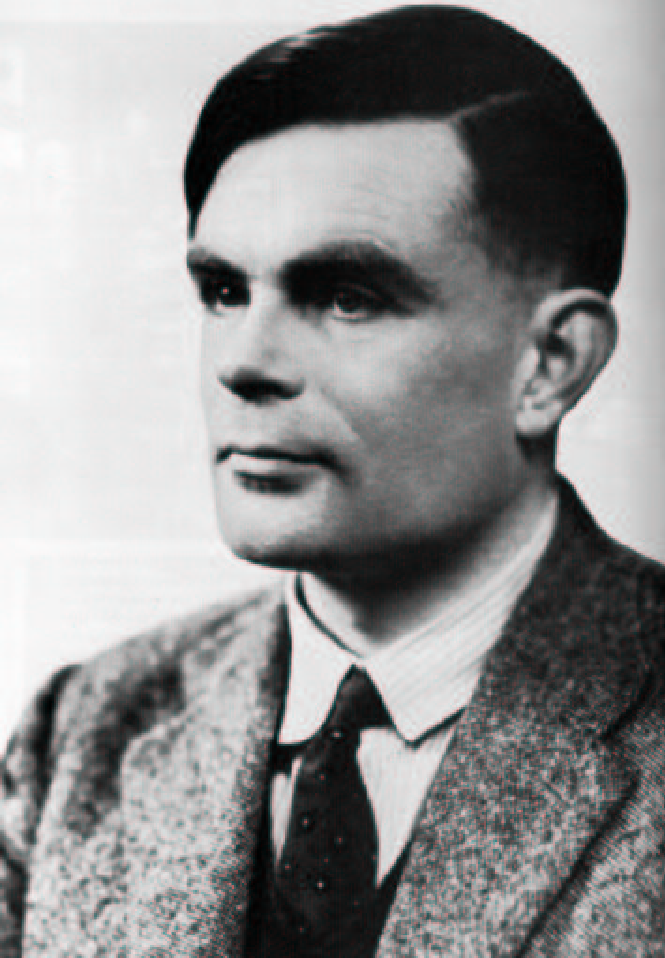
\includegraphics[width=2in]{figures/turing.pdf}}

The man pictured above is Alan Turing, the most important figure in
the history of computer science.  For decades, his fascinating life
story was shrouded by government secrecy, societal taboo, and even his
own deceptions.

At 24 Turing wrote a paper entitled \textit{On Computable Numbers, with an
Application to the Entscheidungsproblem}.  The crux of the paper was an
elegant way to model a computer in mathematical terms.  This was a
breakthrough, because it allowed the tools of mathematics to be brought to
bear on questions of computation.  For example, with his model in hand,
Turing immediately proved that there exist problems that no computer can
solve--- no matter how ingenious the programmer.  Turing's paper is all the
more remarkable because he wrote it in 1936, a full decade before any
electronic computer actually existed.

The word ``Entscheidungsproblem'' in the title refers to one of the 28
mathematical problems posed by David Hilbert in 1900 as challenges to
mathematicians of the 20th century.  Turing knocked that one off in
the same paper.  And perhaps you've heard of the ``Church-Turing
thesis''?  Same paper.  So Turing was obviously a brilliant guy who
generated lots of amazing ideas.  But this lecture is about one of
Turing's less-amazing ideas.  It involved codes.  It involved number
theory.  And it was sort of stupid.

%\subsection{Turing's Code}

Let's look back to the fall of 1937.  Nazi Germany was rearming under
Adolf Hitler, world-shattering war looked imminent, and--- like us--- Alan
Turing was pondering the usefulness of number theory.  He foresaw that
preserving military secrets would be vital in the coming conflict and
proposed a way \textit{to encrypt communications using number theory}.
This is an idea that has ricocheted up to our own time.  Today, number
theory is the basis for numerous public-key cryptosystems, digital
signature schemes, cryptographic hash functions, and digital cash systems.
Every time you buy a book from Amazon, check your grades on WebSIS, or use
a PayPal account, you are relying on number theoretic algorithms.
Furthermore, military funding agencies are among the biggest investors in
cryptographic research.  Sorry Hardy!

Soon after devising his code, Turing disappeared from public view, and
half a century would pass before the world learned the full story of
where he'd gone and what he did there.  We'll come back to Turing's
life in a little while; for now, let's investigate the code Turing
left behind.  The details are uncertain, since he never formally
published the idea, so we'll consider a couple of possibilities.

\subsection{Turing's Code (Version 1.0)}

The first challenge is to translate a text message into an integer so
we can perform mathematical operations on it.  This step is not
intended to make a message harder to read, so the details are not too
important.  Here is one approach: replace each letter of the message
with two digits ($A = 01$, $B = 02$, $C = 03$, etc.) and string all
the digits together to form one huge number.  For example, the message
``victory'' could be translated this way:
%
\begin{center}
\begin{tabular}{ccccccccc}
   &``v &  i &  c &  t & o & r & y'' \\
$\rightarrow$ & 22 & 09 & 03 & 20 & 15 & 18 & 25
\end{tabular}
\end{center}
%
Turing's code requires the message to be a prime number, so we may
need to pad the result with a few more digits to make a prime.  In
this case, appending the digits 13 gives the number 2209032015182513,
which is prime.

Now here is how the encryption process works.  In the description
below, $m$ is the unencoded message (which we want to keep secret),
$m^*$ is the encrypted message (which the Nazis may intercept), and
$k$ is the key.

\begin{description}

\item[Beforehand] The sender and receiver agree on a secret key, which
is a large prime $k$.

\item[Encryption] The sender encrypts the message $m$ by computing:
\[
m^* = m \cdot k
\]

\item[Decryption] The receiver decrypts $m^*$ by computing:
\[
\frac{m^*}{k} = \frac{m \cdot k}{k} = m
\]

\end{description}

For example, suppose that the secret key is the prime number $k =
22801763489$ and the message $m$ is ``victory''.  Then the encrypted
message is:
%
\begin{align*}
m^* & = m \cdot k \\
   & = 2209032015182513 \cdot 22801763489 \\
   & = 50369825549820718594667857
\end{align*}

There are a couple of questions that one might naturally ask about Turing's
code.

\begin{enumerate}

\item How can the sender and receiver ensure that $m$ and $k$ are
prime numbers, as required?

The general problem of determining whether a large number is prime or
composite has been studied for centuries, and reasonably good primality
tests were known even in Turing's time.  In 2002, Manindra Agrawal, Neeraj
Kayal, and Nitin Saxena announced a primality test that is guaranteed to
work on a number $n$ in about $(\log n)^{12}$ steps, that is, a number of
steps bounded by a twelfth degree polynomial in the length (in bits) of
the input, $n$.  This definitively places primality testing way below the
problems of exponential difficulty.  Amazingly, the description of their
breakthrough algorithm was only thirteen lines long!

Of course, a twelfth degree polynomial grows pretty fast, so the
Agrawal,\emph{ et al.}\ procedure is of no practical use.  Still, good
ideas have a way of breeding more good ideas, so there's certainly hope
further improvements will lead to a procedure that is useful in practice.
But the truth is, there's no practical need to improve it, since very
efficient \emph{probabilistic} procedures for prime-testing have been
known since the early 1970's.  These procedures have some probability of
giving a wrong answer, but their probability of being wrong is so tiny
that betting on their answers is the best bet you'll ever make.

\item Is Turing's code secure?

The Nazis see only the encrypted message $m^* = m \cdot k$, so
recovering the original message $m$ requires factoring $m^*$.  Despite
immense efforts, no really efficient factoring algorithm has ever been
found.  It appears to be a fundamentally difficult problem, though a
breakthrough someday is not impossible.  In effect, Turing's code puts
to practical use his discovery that there are limits to the power of
computation.  Thus, provided $m$ and $k$ are sufficiently large, the
Nazis seem to be out of luck!

\end{enumerate}

This all sounds promising, but there is a major flaw in Turing's code.

\subsection{Breaking Turing's Code}

Let's consider what happens when the sender transmits a
\textit{second} message using Turing's code and the same key.  This
gives the Nazis two encrypted messages to look at:
%
\[
m_1^* = m_1 \cdot k
\hspace{0.75in} \text{and} \hspace{0.75in}
m_2^* = m_2 \cdot k
\]
%
The greatest common divisor of the two encrypted messages, $m_1^*$ and
$m_2^*$, is the secret key $k$.  And, as we've seen, the $\gcd$ of two
numbers can be computed very efficiently.  So after the second message is
sent, the Nazis can recover the secret key and read \textit{every}
message!

It is difficult to believe a mathematician as brilliant as Turing
could overlook such a glaring problem.  One possible explanation is
that he had a slightly different system in mind, one based on
\textit{modular} arithmetic.

%% Problems %%%%%%%%%%%%%%%%%%%%%%%%%%%%%%%%%%%%%%%%%%%%%%%%%%%%%%%%%%%%%%%%%%%
%\startclassproblems
%\pinput{CP_}


%% Modular Arithmetic %%%%%%%%%%%%%%%%%%%%%%%%%%%%%%%%%%%%%%%%%%%%%%%%%%%%%%%%%
\hyperdef{modular}{arithmetic}{\section{Modular Arithmetic}}
\label{sec:modular-arithmeric}

% Congruence is a weak form of equality.

On page 1 of his masterpiece on number theory, {\em Disquisitiones
Arithmeticae}, Gauss introduced the notion of ``congruence''.  Now,
Gauss is another guy who managed to cough up a half-decent idea every
now and then, so let's take a look at this one.  Gauss said that
\term{$a$ is congruent to $b$ modulo $n$} iff $n \divides (a - b)$.  This
is denoted $a \equiv b \pmod{n}$.  For example:
%
\[
29 \equiv 15 \pmod{7}  \quad\text{ because }  7 \divides (29 - 15).
\]

There is a close connection between congruences and remainders:
\begin{lemma}[Congruences and Remainders]
\label{lem:conrem}
\[
a \equiv b \pmod{n} \qiff \rem{a}{n} = \rem{b}{n}.
\]
\end{lemma}

\begin{proof}
By the Division Theorem, there exist unique pairs of integers $q_1, r_1$
and $q_2, r_2$ such that:
%
\begin{align*}
a & = q_1 n + r_1 & \text{where $0 \leq r_1 < n$}, \\
b & = q_2 n + r_2 & \text{where $0 \leq r_2 < n$}.
\end{align*}
%
In these terms, $\rem{a}{n} = r_1$ and $\rem{b}{n} = r_2$.
Subtracting the second equation from the first gives:
%
\begin{align*}
a - b & = (q_1 - q_2) n + (r_1 - r_2)
  & \text{where $-n < r_1 - r_2 < n$}.
\end{align*}
%
Now $a \equiv b \pmod{n}$ if and only if $n$ divides the left side.
This is true if and only if $n$ divides the right side, which holds if
and only if $r_1 - r_2$ is a multiple of $n$.  Given the bounds on
$r_1 - r_2$, this happens precisely when $r_1 = r_2$, which is
equivalent to $\rem{a}{n} = \rem{b}{n}$.
\end{proof}

So we can also see that
\[
29 \equiv 15 \pmod{7} \quad\text{ because } \rem{29}{7} = 1 = \rem{15}{7}.
\]
This formulation explains why the congruence relation has properties like
an equality relation.  Notice that even though (mod 7) appears over on the
right side the $\equiv$ symbol, it is in no sense more strongly associated
with the 15 than the 29.  It would really be clearer to write $29
\equiv_{\mod 7} 15$ for example, but the notation with the modulus at the
end is firmly entrenched and we'll stick to it.

We'll make frequent use of the following immediate Corollary of
Lemma~\ref{lem:conrem}:
\begin{corollary}\label{aran}
\[
a \equiv \rem{a}{n} \pmod{n}
\]
\end{corollary}

Still another way to think about congruence modulo $n$ is that it
\emph{defines a partition of the integers into $n$ sets so that congruent
numbers are all in the same set}.  For example, suppose that we're working
modulo 3.  Then we can partition the integers into 3 sets as follows:
%
\[
\begin{array}{cccccccccc}
\{ & \dots, & -6, & -3, & 0, & 3, & 6, & 9, & \dots & \} \\
\{ & \dots, & -5, & -2, & 1, & 4, & 7, & 10, & \dots & \} \\
\{ & \dots, & -4, & -1, & 2, & 5, & 8, & 11, & \dots & \}
\end{array}
\]
according to whether their remainders on division by 3 are 0, 1, or 2.
The upshot is that when arithmetic is done modulo $n$ there are really
only $n$ different kinds of numbers to worry about, because there are only
$n$ possible remainders.  In this sense, modular arithmetic is a
simplification of ordinary arithmetic and thus is a good reasoning tool.

There are many useful facts about congruences, some of which are listed in
the lemma below.  The overall theme is that \textit{congruences work a lot
like equations}, though there are a couple of exceptions.

\begin{lemma}[Facts About Congruences]  The following  hold for 
$n \geq 1$:
%
\begin{enumerate}
\item $a \equiv a \pmod{n}$
\item $a \equiv b \pmod{n}$ implies $b \equiv a \pmod{n}$
\item $a \equiv b \pmod{n}$ and $b \equiv c \pmod{n}$ implies $a \equiv c \pmod{n}$
\item $a \equiv b \pmod{n}$ implies $a + c \equiv b + c \pmod{n}$
\item $a \equiv b \pmod{n}$ implies $a c \equiv b c \pmod{n}$
\item $a \equiv b \pmod{n}$ and $c \equiv d \pmod{n}$ imply $a + c
\equiv b + d \pmod{n}$
\item $a \equiv b \pmod{n}$ and $c \equiv d \pmod{n}$ imply $a c
\equiv b d \pmod{n}$
\end{enumerate}
\end{lemma}

\begin{proof}
Parts 1.--3.\ follow immediately from Lemma~\ref{lem:conrem}.  Part 4.\
follows immediately from the definition that $a \equiv b \pmod{n}$ iff $n
\divides (a-b)$.  Likewise, part 5.\ follows because if $n \divides (a-b)$
then it divides $(a-b)c = ac - bc$.  To prove part 6., assume
\begin{equation}\label{ab}
a \equiv b \pmod{n}
\end{equation}
and
\begin{equation}\label{cd}
c \equiv d \pmod{n}.
\end{equation}
Then
\begin{align*}
a + c & \equiv b + c \pmod{n} & \text{(by part 4.\ and~\eqref{ab}}),\\
c + b & \equiv d + b \pmod{n} & \text{(by part 4.\ and~\eqref{cd}), so}\\
b + c & \equiv b + d \pmod{n} & \text{and therefore}\\
a + c & \equiv b + d \pmod{n} & \text{(by part 3.)}
\end{align*}
Part 7.\ has a similar proof.
\end{proof}

\iffalse

There is a close connection between modular arithmetic and the
remainder operation, which we looked at last time.  To clarify this
link, let's reconsider the partition of the integers defined by
congruence modulo 3:
%
\[
\begin{array}{cccccccccc}
\{ & \dots, & -6, & -3, & 0, & 3, & 6, & 9, & \dots & \} \\
\{ & \dots, & -5, & -2, & 1, & 4, & 7, & 10, & \dots & \} \\
\{ & \dots, & -4, & -1, & 2, & 5, & 8, & 11, & \dots & \}
\end{array}
\]
%
Notice that two numbers are in the same set if and only if they leave
the same remainder when divided by 3.  The numbers in the first set
all leave a remainder of 0 when divided by 3, the numbers in the
second set leave a remainder of 1, and the numbers in the third leave
a remainder of 2.  Furthermore, notice that each number is in the same
set as its own remainder.  For example, 11 and $\rem{11}{3} = 2$ are
both in the same set.  Let's bundle all this happy goodness into a
lemma.
\fi

\TBA{put in 'example' environment}

\subsection{Turing's Code (Version 2.0)}

In 1940 France had fallen before Hitler's army, and Britain alone stood
against the Nazis in western Europe.  British resistance depended on a
steady flow of supplies brought across the north Atlantic from the United
States by convoys of ships.  These convoys were engaged in a cat-and-mouse
game with German ``U-boats'' ---submarines ---which prowled the Atlantic,
trying to sink supply ships and starve Britain into submission.  The
outcome of this struggle pivoted on a balance of information: could the
Germans locate convoys better than the Allies could locate U-boats or vice
versa?

Germany lost.

But a critical reason behind Germany's loss was made public only in
1974: the British had broken Germany's naval code, Enigma.  Through
much of the war, the Allies were able to route convoys around German
submarines by listening into German communications.  The British
government didn't explain \textit{how} Enigma was broken until 1996.
When the analysis was finally released (by the US), the author was
none other than Alan Turing.  In 1939 he had joined the secret British
codebreaking effort at Bletchley Park.  There, he played a central
role in cracking the German's Enigma code and thus in preventing
Britain from falling into Hitler's hands.

Governments are always tight-lipped about cryptography, but the
half-century of official silence about Turing's role in breaking
Enigma and saving Britain may be related to some disturbing events
after the war.

Let's consider an alternative interpretation of Turing's code.
Perhaps we had the basic idea right (multiply the message by the key),
but erred in using \textit{conventional} arithmetic instead of
\textit{modular} arithmetic.  Maybe this is what Turing meant:
%
\begin{description}

\item[Beforehand] The sender and receiver agree on a large prime $p$,
which may be made public.  (This will be the modulus for all our
arithmetic.)  They also agree on a secret key $k \in \set{1, 2,
\dots, p-1}$.

\item[Encryption] The message $m$ can be any integer in the set
$\set{0, 1, 2, \dots, p-1}$; in particular, the message is no longer
required to be a prime.  The sender encrypts the message $m$ to
produce $m^*$ by computing:
%
\begin{equation}
m^* = \rem{mk}{p} \label{eq:turing-code}
\end{equation}

\item[Decryption] (Uh-oh.)

\end{description}

The decryption step is a problem.  We might hope to decrypt in the
same way as before: by dividing the encrypted message $m^*$ by the key
$k$.  The difficulty is that $m^*$ is the \textit{remainder} when $mk$
is divided by $p$.  So dividing $m^*$ by $k$ might not even give us an
integer!

This decoding difficulty can be overcome with a better understanding
of arithmetic modulo a prime.

%% Problems %%%%%%%%%%%%%%%%%%%%%%%%%%%%%%%%%%%%%%%%%%%%%%%%%%%%%%%%%%%%%%%%%%%
%\startclassproblems
\pinput{CP_proving_basic_congruence_properties}
\pinput{CP_multiples_of_9_and_11}
\pinput{CP_nonparallel_lines}
\pinput{CP_13th_roots}

%% Arithmetic with a Prime Modulus %%%%%%%%%%%%%%%%%%%%%%%%%%%%%%%%%%%%%%%%%%%%
\section{Arithmetic with a Prime Modulus}

\subsection{Multiplicative Inverses}
\label{sec:prime}

The \term{multiplicative inverse} of a number $x$ is another number
$x^{-1}$ such that:
%
\[
x \cdot x^{-1} = 1
\]

Generally, multiplicative inverses exist over the real numbers.  For
example, the multiplicative inverse of 3 is $1 / 3$ since:
%
\[
3 \cdot \frac{1}{3} = 1
\]
%
The sole exception is that 0 does not have an inverse.

On the other hand, inverses generally do not exist over the integers.
For example, 7 can not be multiplied by another integer to give 1.

Surprisingly, multiplicative inverses do exist when we're working
\textit{modulo a prime number}.  For example, if we're working modulo
5, then 3 is a multiplicative inverse of 7, since:
%
\[
7 \cdot 3 \equiv 1 \pmod{5}
\]
%
(All numbers congruent to 3 modulo 5 are also multiplicative inverses
of 7; for example, $7 \cdot 8 \equiv 1 \pmod{5}$ as well.)  The only
exception is that numbers congruent to 0 modulo 5 (that is, the
multiples of 5) do not have inverses, much as 0 does not have an
inverse over the real numbers.  Let's prove this.

\begin{lemma}
\label{lem:inverses}
If $p$ is prime and $k$ is not a multiple of $p$, then $k$ has a
multiplicative inverse.
\end{lemma}

\begin{proof}
Since $p$ is prime, it has only two divisors: 1 and $p$.  And since
$k$ is not a multiple of $p$, we must have $\gcd(p, k) = 1$.
Therefore, there is a linear combination of $p$ and $k$ equal to 1:
%
\[
s p + t k = 1
\]
%
Rearranging terms gives:
%
\[
s p = 1 - t k
\]
%
This implies that $p \divides \paren{1 - tk}$ by the definition of divisibility,
and therefore $tk \equiv 1 \pmod{p}$ by the definition of congruence.
Thus, $t$ is a multiplicative inverse of $k$.
\end{proof}

Multiplicative inverses are the key to decryption in Turing's code.
Specifically, we can recover the original message by multiplying the
encoded message by the \textit{inverse} of the key:
\begin{align*}
m^* \cdot k^{-1}
    & = \rem{mk}{p} \cdot k^{-1}
         & \text{(def.~\eqref{eq:turing-code} of $m^*$)}\\
    & \equiv (mk)k^{-1} \pmod{p} & \text{(by Cor.~\ref{aran})}\\
    & \equiv m \pmod{p}.
\end{align*}

This shows that $m^* k^{-1}$ is congruent to the original message $m$.
Since $m$ was in the range $0, 1, \dots, p - 1$, we can recover
it exactly by taking a remainder:
%
\[
m = \rem{m^* k^{-1}}{p}
\]
%
So now we can decrypt!

\subsection{Cancellation}

Another sense in which real numbers are nice is that one can cancel
multiplicative terms.  In other words, if we know that $m_1 k = m_2 k$,
then we can cancel the $k$'s and conclude that $m_1 = m_2$, provided $k
\neq 0$.  In general, cancellation is \textit{not} valid in modular
arithmetic.  For example, this congruence is correct:
%
\[
2 \cdot 3 \equiv 4 \cdot 3 \pmod{6}
\]
%
But if we cancel the 3's, we reach a false conclusion:
%
\[
2 \equiv 4 \pmod{6}
\]
%
The fact that multiplicative terms can not be cancelled is the most
significant sense in which congruences differ from ordinary equations.
However, this difference goes away if we're working modulo a
\textit{prime}; then cancellation is valid.

\begin{lemma}
\label{lem:cancel}
Suppose $p$ is a prime and $k$ is not a multiple of $p$.  Then
%
\[
ak \equiv bk \pmod{p}
\hspace{0.5in} \text{implies} \hspace{0.5in}
a \equiv b \pmod{p}
\]
\end{lemma}

\begin{proof}
Multiply both sides of the congruence by $k^{-1}$.
\end{proof}

We can use this lemma to get a bit more insight into how Turing's code
works.  In particular, the encryption operation in Turing's code
\textit{permutes the set of possible messages}.  This is stated more
precisely in the following corollary.

\hyperdef{for}{Fermat}{\begin{corollary}
\label{cor:prime-permutes}
Suppose $p$ is a prime and $k$ is not a multiple of $p$.  Then the
sequence:
\[
\rem{(0 \cdot k)}{p},\quad
\rem{(1 \cdot k)}{p},\quad
\rem{(2 \cdot k)}{p},\quad
 \dots,\quad
\rem{\paren{(p-1) \cdot k}}{p}
\]
is a permutation\footnote{A \emph{permutation} of a sequence of elements
is a sequence with the same elements (including repeats) possibly in a
different order.  More formally, if
\[
\vec{e} \eqdef e_1,e_2,\dots,e_n
\]
is a length $n$ sequence, and  $\pi: \set{1,\dots, n} \to \set{1,\dots,
n}$ is a bijection, then
\[
e_{\pi(1)}, e_{\pi(2)},\dots, e_{\pi(n)},
\]
is a \emph{permutation} of $\vec{e}$.} of the sequence:
\[
0,\quad 1,\quad 2,\quad \dots,\quad (p - 1)
\]
This remains true if the first term is deleted from each sequence.
\end{corollary}}

\begin{proof}
The first sequence contains $p$ numbers, which are all in the range
$0$ to $p - 1$ by the definition of remainder.  Furthermore, the
numbers in the first sequence are all different; by
Lemma~\ref{lem:cancel}, $i k \equiv j k \pmod{p}$
if and only if $i \equiv j \pmod{p}$, and no two numbers in the range 0, 1,
\dots, p - 1 are congruent modulo $p$.  Thus, the first sequence must
contain \textit{all} of the numbers from 0 to $p - 1$ in some order.
The claim remains true if the first terms are deleted, because both
sequences begin with 0.
\end{proof}

For example, suppose $p = 5$ and $k = 3$.  Then the sequence:
%
\[
\underbrace{\rem{(0 \cdot 3)}{5}}_{=0},\quad
\underbrace{\rem{(1 \cdot 3)}{5}}_{=3},\quad
\underbrace{\rem{(2 \cdot 3)}{5}}_{=1},\quad
\underbrace{\rem{(3 \cdot 3)}{5}}_{=4},\quad
\underbrace{\rem{(4 \cdot 3)}{5}}_{=2}
\]
%
is a permutation of 0, 1, 2, 3, 4 and the last four terms are a
permutation of 1, 2, 3, 4.  As long as the Nazis don't know the secret key
$k$, they don't know how the set of possible messages are permuted by the
process of encryption and thus can't read encoded messages.

%%%%%%%%%%%%%%%%%%%%%%%%%%%%%%%%%%%%%%%%%%%%%%%%%%%%%%%%%%%%%%%%%%%%%%%%%%%%%%%

\subsection{Fermat's Theorem}

A remaining challenge in using Turing's code is that decryption requires
the inverse of the secret key $k$.  An effective way to calculate
$k^{-1}$ follows from the proof of Lemma~\ref{lem:inverses}: $k^{-1} =
\rem{t}{p}$ where $s,t$ are coefficients such that $sp+tk=1$.  Notice that
$t$ is easy to find using the Pulverizer.

An alternative approach, about equally efficient and probably more
memorable, is to rely on Fermat's Theorem, which is much easier than his
famous Last Theorem ---and more useful.

\begin{theorem}[Fermat's Theorem]
Suppose $p$ is a prime and $k$ is not a multiple of $p$.  Then:
%
\[
k^{p-1} \equiv 1 \pmod{p}
\]
\end{theorem}

\begin{proof}
We reason as follows:
\begin{align*}
1 \cdot 2 \cdots (p-1)
	& = \rem{k}{p} \cdot \rem{2k}{p} \cdots
	\rem{(p-1)k}{p} & \text{(by Cor~\ref{cor:prime-permutes})}\\
	& \equiv k \cdot 2k \cdots (p-1) k \pmod{p}
            & \text{(by Cor~\ref{aran})}\\
	& \equiv (p-1)! \cdot k^{p-1} \pmod{p} & \text{(rearranging terms)}\\
\end{align*}

Now $(p - 1)!$ can not be a multiple of $p$, because the prime
factorizations of $1, 2, \dots, (p - 1)$ contain only primes smaller
than $p$.  Therefore, we can cancel $(p - 1)!$ from the first
expression and the last by Lemma~\ref{lem:cancel}, which proves the
claim.
\end{proof}

Here is how we can find inverses using Fermat's Theorem.  Suppose $p$
is a prime and $k$ is not a multiple of $p$.  Then, by Fermat's
Theorem, we know that:
%
\[
k^{p-2} \cdot k \equiv 1 \pmod{p}
\]
%
Therefore, $k^{p-2}$ must be a multiplicative inverse of $k$.  For
example, suppose that we want the multiplicative inverse of 6 modulo
17.  Then we need to compute $\rem{6^{15}}{17}$, which we can do by
successive squaring.  All the congruences below hold modulo 17.
%
\begin{align*}
6^2 & \equiv 36 \equiv 2 \\
6^4 & \equiv (6^2)^2 \equiv 2^2 \equiv 4 \\
6^8 & \equiv (6^4)^2 \equiv 4^2 \equiv 16 \\
6^{15} & \equiv 6^8 \cdot 6^4 \cdot 6^2 \cdot 6
       \equiv 16 \cdot 4 \cdot 2 \cdot 6
       \equiv 3
\end{align*}
%
Therefore, $\rem{6^{15}}{17} = 3$.  Sure enough, 3 is the multiplicative
inverse of 6 modulo 17, since:
%
\[
3 \cdot 6 \equiv 1 \pmod{17}
\]

In general, if we were working modulo a prime $p$, finding a
multiplicative inverse by trying every value between 1 and $p - 1$
would require about $p$ operations.  However, the approach above
requires only about $\log p$ operations, which is far better when $p$
is large.

\subsection{Breaking Turing's Code--- Again}

The Germans didn't bother to encrypt their weather reports with the
highly-secure Enigma system.  After all, so what if the Allies learned
that there was rain off the south coast of Iceland?  But, amazingly, this
practice provided the British with a critical edge in the Atlantic naval
battle during 1941.

The problem was that some of those weather reports had originally been
transmitted from U-boats out in the Atlantic.  Thus, the British
obtained both unencrypted reports and the same reports encrypted with
Enigma.  By comparing the two, the British were able to determine
which key the Germans were using that day and could read all other
Enigma-encoded traffic.  Today, this would be called a
\term{known-plaintext attack}.

Let's see how a known-plaintext attack would work against Turing's
code.  Suppose that the Nazis know both $m$ and $m^*$ where:
%
\[
m^* \equiv mk \pmod{p}
\]
%
Now they can compute:
%
\begin{align*}
m^{p-2} \cdot m^*
  & = m^{p-2} \cdot \rem{mk}{p}
                & \text{(def.~\eqref{eq:turing-code} of $m^*$)}\\
  & \equiv m^{p-2} \cdot mk \pmod{p} & \text{(by Cor~\ref{aran})}\\
  & \equiv m^{p-1} \cdot k \pmod{p}\\ % & \text{(simplification)}\\
  & \equiv k \pmod{p} & \text{(Fermat's Theorem)}
\end{align*}
%
Now the Nazis have the secret key $k$ and can decrypt any message!

This is a huge vulnerability, so Turing's code has no practical value.
Fortunately, Turing got better at cryptography after devising this
code; his subsequent cracking of Enigma surely saved thousands of
lives, if not the whole of Britain.

%  I could insert a bit about public-key cryptography here as introduction to
%  the recitation.

\subsection{Turing Postscript}

A few years after the war, Turing's home was robbed.  Detectives soon
determined that a former homosexual lover of Turing's had conspired in the
robbery.  So they arrested him ---that is, they arrested Alan Turing
---because homosexuality was a British crime punishable by up to two years
in prison at that time.  Turing was sentenced to a humiliating hormonal
``treatment'' for his homosexuality: he was given estrogen injections.  He
began to develop breasts.

Three years later, Alan Turing, the founder of computer science, was
dead.  His mother explained what happened in a biography of her own
son.  Despite her repeated warnings, Turing carried out chemistry
experiments in his own home.  Apparently, her worst fear was realized:
by working with potassium cyanide while eating an apple, he poisoned
himself.

However, Turing remained a puzzle to the very end.  His mother was a
devoutly religious woman who considered suicide a sin.  And, other
biographers have pointed out, Turing had previously discussed
committing suicide by eating a poisoned apple.  Evidently, Alan
Turing, who founded computer science and saved his country, took his
own life in the end, and in just such a way that his mother could
believe it was an accident.


\floatingtextbox{
\textboxtitle{The Riemann Hypothesis}

Turing's last project before he disappeared from public view in 1939
involved the construction of an elaborate mechanical device to test a
mathematical conjecture called the Riemann Hypothesis.  This conjecture
first appeared in a sketchy paper by Berhard Riemann in 1859 and is now
one of the most famous unsolved problem in mathematics.  The formula for
the sum of an infinite geometric series says:
\[
1 + x + x^2 + x^3 + \cdots = \frac{1}{1-x}
\]
Substituting $x = \frac{1}{2^s}$, $x = \frac{1}{3^s}$, 
$x = \frac{1}{5^s}$, and so on for each prime
number gives a sequence of equations:
%
\begin{align*}
1 + \frac{1}{2^s} + \frac{1}{2^{2s}} + \frac{1}{2^{3s}} + \cdots
    & = \frac{1}{1 - 1 / 2^s} \\
1 + \frac{1}{3^s} + \frac{1}{3^{2s}} + \frac{1}{3^{3s}} + \cdots
    & = \frac{1}{1 - 1 / 3^s} \\
1 + \frac{1}{5^s} + \frac{1}{5^{2s}} + \frac{1}{5^{3s}} + \cdots
    & = \frac{1}{1 - 1 / 5^s} \\
    & \text{etc.}
\end{align*}
%
Multiplying together all the left sides and all the right sides gives:
%
\[
\sum_{n=1}^{\infty} \frac{1}{n^s} = \prod_{p \in \text{primes}} \left(\frac{1}{1 - 1 / p^s}\right)
\]
%
The sum on the left is obtained by multiplying out all the infinite
series and applying the Fundamental Theorem of Arithmetic.  For
example, the term $1 / 300^s$ in the sum is obtained by multiplying $1
/ 2^{2s}$ from the first equation by $1 / 3^s$ in the second and $1 /
5^{2s}$ in the third.  Riemann noted that every prime appears in the
expression on the right.  So he proposed to learn about the primes by
studying the equivalent, but simpler expression on the left.  In
particular, he regarded $s$ as a complex number and the left side as a
function, $\zeta(s)$.  Riemann found that the distribution of primes
is related to values of $s$ for which $\zeta(s) = 0$, which led to his
famous conjecture:
\begin{quote}
\emph{The Riemann Hypothesis}: Every nontrivial zero of the zeta function
$\zeta(s)$ lies on the line $s = 1/2 + c i$ in the complex plane.
\end{quote}

Researchers continue to work intensely to settle this conjecture, as they
have for over a century.  A proof would immediately imply, among other
things, a strong form of the Prime Number Theorem--- and earn the prover a
\$1 million prize!  (We're not sure what the cash would be for a
counter-example, but the discoverer would be wildly applauded by
mathematicians everywhere.)}

%% Problems %%%%%%%%%%%%%%%%%%%%%%%%%%%%%%%%%%%%%%%%%%%%%%%%%%%%%%%%%%%%%%%%%%%
%\startclassproblems
\pinput{CP_Sk_equiv_-1_mod_p}


%% Arithmetic with an Arbitrary Modulus %%%%%%%%%%%%%%%%%%%%%%%%%%%%%%%%%%%%%%%
\hyperdef{mod}{n}{\section{Arithmetic with an Arbitrary Modulus}}

Turing's code did not work as he hoped.  However, his essential
idea--- using number theory as the basis for cryptography--- succeeded
spectacularly in the decades after his death.

In 1977, Ronald Rivest, Adi Shamir, and Leonard Adleman at MIT proposed a
highly secure cryptosystem (called \textbf{RSA}) based on number theory.
Despite decades of attack, no significant weakness has been found.
Moreover, RSA has a major advantage over traditional codes: the sender and
receiver of an encrypted message need not meet beforehand to agree on a
secret key.  Rather, the receiver has both a \term{secret key}, which she
guards closely, and a \term{public key}, which she distributes as widely
as possible.  To send her a message, one encrypts using her
widely-distributed public key.  Then she decrypts the message using her
closely-held private key.  The use of such a \term{public key
cryptography} system allows you and Amazon, for example, to engage in a
secure transaction without meeting up beforehand in a dark alley to
exchange a key.

Interestingly, RSA does not operate modulo a prime, as Turing's scheme
may have, but rather modulo the product of \textit{two} large primes.
Thus, we'll need to know a bit about how arithmetic works modulo a
composite number in order to understand RSA.  Arithmetic modulo an
arbitrary positive integer is really only a little more painful than
working modulo a prime, in the same sense that a doctor says ``This is
only going to hurt a little'' before he jams a big needle in your arm.

\subsection{Relative Primality and Phi}

First, we need a new definition.  Integers $a$ and $b$ are
\term{relatively prime} iff $\gcd(a, b) = 1$.  For example, 8 and 15
are relatively prime, since $\gcd(8, 15) = 1$.  Note that every
integer is relatively prime to a genuine prime number $p$, except for
multiples of $p$.

We'll also need a certain function that is defined using relative
primality.  Let $n$ be a positive integer.  Then $\phi(n)$ denotes the
number of integers in $\set{1, 2, \dots, n - 1}$ that are relatively
prime to $n$.  For example, $\phi(7) = 6$, since 1, 2, 3, 4, 5, and 6
are all relatively prime to 7.  Similarly, $\phi(12) = 4$, since only
1, 5, 7, and 11 are relatively prime to 12.  If you know the prime
factorization of $n$, then computing $\phi(n)$ is a piece of cake,
thanks to the following theorem.

\begin{theorem}
\label{th:phi}
The function $\phi$ obeys the following relationships:
\begin{enumerate}
\item[(a)] If $a$ and $b$ are relatively prime, then $\phi(ab) = \phi(a)\phi(b)$.
\item[(b)] If $p$ is a prime, then $\phi(p^k) = p^k - p^{k-1}$ for $k \geq 1$.
\end{enumerate}
\end{theorem}

Here's an example of using Theorem~\ref{th:phi} to compute $\phi(300)$:
%
\begin{align*}
\phi(300)
    & = \phi(2^2 \cdot 3 \cdot 5^2)\\
    & = \phi(2^2) \cdot \phi(3) \cdot \phi(5^2)
            & \text{(by Theorem~\ref{th:phi}.(a))}\\
    & = (2^2 - 2^1) (3^1 - 3^0) (5^2 - 5^1) 
            & \text{(by Theorem~\ref{th:phi}.(b))}\\
    & = 80.
\end{align*}
\iffalse
We factor 300 in the first step, use part (1) of Theorem~\ref{th:phi}
twice in the second step, use part (2) in the third step, and then
simplify.
\fi

We'll work out a proof of Theorem~\ref{th:phi}.(a) in the next
section, after we've work out a few more properties of modular arithmetic.
We'll also give another a proof in a few weeks based on rules for counting
things.

To prove Theorem~\ref{th:phi}.(b), notice that the numbers in the interval
from 0 to $p^{k}-1$ that are divisible by $p$ are all those of the form
$mp$.  For $mp$ to be in the interval, $m$ can take any value from 0 to
$p^{k-1}-1$ and no others, so there are exactly $p^{k-1}$ numbers in the
interval that are divisible by $p$.  Now $\phi(p^{k})$ equals the number
of remaining elements in the interval, namely, $p^k -p^{k-1}$.


\subsection{Generalizing to an Arbitrary Modulus}

Let's generalize what we know about arithmetic modulo a prime.  Now,
instead of working modulo a prime $p$, we'll work modulo an arbitrary
positive integer $n$.  The basic theme is that arithmetic modulo $n$ may
be complicated, but the integers {\em relatively prime} to $n$ remain
fairly well-behaved.  For example, the proof of Lemma~\ref{lem:inverses}
of an inverse for $k$ modulo $p$ extends to an inverse for $k$ relatively
prime to $n$:

\begin{lemma}
\label{lem:inverse-arb}
Let $n$ be a positive integer.  If $k$ is relatively prime to $n$,
then there exists an integer $k^{-1}$ such that:
%
\[
k \cdot k^{-1} \equiv 1 \pmod{n}
\]
\end{lemma}


\iffalse
\begin{proof}
There exist integers $s$ and $t$ such that $s k + t n = \gcd(k, n) =
1$ by Theorem~\ref{th:gcd}.  Rearranging terms gives $tn = 1 - sk$,
which implies that $n \divides 1 - sk$ and $sk \equiv 1 \pmod{n}$.  Define
$k^{-1}$ to be $s$.
\end{proof}
\fi

As a consequence of this lemma, we can cancel a multiplicative term
from both sides of a congruence if that term is relatively prime to
the modulus:

\begin{corollary}
\label{cor:cancellation-arb}
Suppose $n$ is a positive integer and $k$ is relatively prime to $n$.
If
%
\[
a k \equiv b k \pmod{n}
\]
%
then
%
\[
a \equiv b \pmod{n}
\]
\end{corollary}

This holds because we can multiply both sides of the first congruence
by $k^{-1}$ and simplify to obtain the second.

\subsection{Euler's Theorem}

RSA essentially relies on Euler's Theorem, a generalization of
Fermat's Theorem to an arbitrary modulus.  The proof is much like the
proof of Fermat's Theorem, except that we focus on integers relatively
prime to the modulus.  Let's start with a lemma.

\begin{lemma}
\label{lem:permutes-arb}
Suppose $n$ is a positive integer and $k$ is relatively prime to $n$.
Let $k_1, \dots, k_r$ denote all the integers relatively prime to $n$
in the range $0 \leq k_i < n$.  Then the sequence:
%
\[
\rem{k_1 \cdot k}{n},\quad
\rem{k_2 \cdot k}{n},\quad
\rem{k_3 \cdot k}{n},\quad
\quad \dots\quad,
\rem{k_r \cdot k}{n}
\]
%
is a permutation of the sequence:
%
\[
k_1,\quad k_2,\quad \dots\quad, k_r.
\]
\end{lemma}

\begin{proof}
We will show that the numbers in the first sequence are all distinct
and all appear in the second sequence.  Since the two sequences have
the same length, the first must be a permutation of the second.

First, we show that the numbers in the first sequence are all
distinct.  Suppose that $\rem{k_i k}{n} = \rem{k_j k}{n}$.  This is
equivalent to $k_i k \equiv k_j k \pmod{n}$, which implies $k_i \equiv
k_j \pmod{n}$ by Corollary~\ref{cor:cancellation-arb}.  This, in turn,
means that $k_i = k_j$ since both are between 1 and $n-1$.  Thus, a
term in the first sequence is not equal to any other term.

Next, we show that each number in the first sequence appears in the
second.  By assumption, $\gcd(k_i, n) = 1$ and $\gcd(k, n) = 1$, which
means that
%
\begin{align*}
\gcd(n, \rem{k_i k}{n}) & = \gcd(k_i k, n)
            & \text{(by Lemma~\ref{lem:gcd}.\ref{gcd5})}\\
      & = 1 & \text{(by Lemma~\ref{lem:gcd}.\ref{gcd3})}.
\end{align*}
%
So $\rem{k_i k}{n}$ is relatively prime to $n$ and is in the range from 0
to $n - 1$ by the definition of remainder.  The second sequence is defined
to consist of all such integers.
\end{proof}

We can now prove Euler's Theorem:

\begin{theorem}[Euler's Theorem]
Suppose $n$ is a positive integer and $k$ is relatively prime to $n$.
Then
\begin{eqnarray*}
k^{\phi(n)} \equiv 1 \pmod{n}
\end{eqnarray*}
\end{theorem}

\begin{proof}
Let $k_1, \dots, k_r$ denote all integers relatively prime to $n$
such that $0 \leq k_i < n$.  Then $r = \phi(n)$, by the definition of
the function $\phi$.  Now we can reason as follows:
%
\begin{align*}
\lefteqn{k_1 \cdot k_2 \cdots k_r} \hspace{0.25in} \\
& =
\rem{k_1 \cdot k}{n} \cdot 
\rem{k_2 \cdot k}{n} \cdots 
\rem{k_r \cdot k}{n} & \text{(by Lemma~\ref{lem:permutes-arb})}
\\
& \equiv 
(k_1 \cdot k) \cdot 
(k_2 \cdot k) \cdot 
\cdots 
(k_r \cdot k) \pmod{n} & \text{(by Cor~\ref{aran})}
\\
& \equiv  
(k_1 \cdot k_2 \cdots k_r) \cdot k^r \pmod{n} & \text{(rearranging terms)}
\end{align*}

Lemma~\ref{lem:gcd}.\ref{gcd3}.\ implies that $k_1 \cdot k_2
\cdots k_r$ is prime relative to $n$.  Therefore, we can cancel this
product from the first expression and the last by
Corollary~\ref{cor:cancellation-arb}.  This proves the claim.
\end{proof}

We can find multiplicative inverses using Euler's theorem as we did
with Fermat's theorem: if $k$ is relatively prime to $n$, then
$k^{\phi(n) - 1}$ is a multiplicative inverse of $k$ modulo $n$.
However, this approach requires computing $\phi(n)$.  Our best method
for doing so requires factoring $n$, which can be quite difficult in
general.  Fortunately, when we know how to factor $n$, we can
use Theorem~\ref{th:phi} to compute $\phi(n)$ efficiently!

\begin{notesproblem}\label{phi2}
This problem provides the remaining proof of Theorem~\ref{th:phi}.(a).

Suppose $m,n$ are relatively prime.

\bparts

\ppart Prove that for any $a,b$, there is an
$x$ such that
\begin{align}
x \equiv & a \pmod{m}, \label{xa}\\
x \equiv & b \pmod{n} \label{xb}.
\end{align}

\hint Congruence~\eqref{xa} holds iff
\begin{equation}\label{xj}
x = jm + a.
\end{equation}
for some $j$.  So there is such an $x$ only if
\begin{equation}\label{jn}
j m +a \equiv b \pmod{n}.
\end{equation}
Solve~\eqref{jn} for $j$.

\solution{
\begin{proof}
\footnote{Adapted from
\href{http://www.cut-the-knot.org/blue/chinese.shtml}{\texttt{http://www.cut-the-knot.org/blue/chinese.shtml}}.}
Since $m,n$ are relatively prime, there is an inverse, $m'$, modulo $n$ of
$m$.  So $j = m'(b-a)$ satisfies~\eqref{jn}.  Now~\eqref{xj} leads to the
definition
\[
x_1 \eqdef m'(b-a)m + a.
\]
So
\[
x_1 = (m'(b-a))m + a \equiv a \pmod{m}, 
\]
and
\[
x_1 = m'(b-a)m + a = m'm(b-a) +a \equiv 1\cdot(b-a) + a \equiv b \pmod{n},
\]
proving that $x_1$ satisfies the congruences~\eqref{xa} and~\eqref{xb}.
\end{proof}}

\ppart\label{x0} Prove that there is an $x$ satisfying the
congruences~\eqref{xa} and~\eqref{xb} such that $0 \leq x < mn$.

\solution{
Let
\[
x_0 \eqdef \rem{x_1}{mn},
\]
where $x_1$ satisfies~\eqref{xa} and~\eqref{xb}.

Now $0 \leq x_0 < mn$ by definition of remainder.  Further, we know $x_0
\equiv x_1 \pmod{mn}$, which immediately implies that $x_0 \equiv x_1 \pmod{m}$ and $x_0 \equiv x_1 \pmod{n}$.  So $x_0$ also satisifies~\eqref{xa}
and~\eqref{xb}, and is therefore the desired solution.
}

\ppart\label{uniq} Prove that the $x$ satisfying part~\eqref{x0} is unique.

\solution{Assume $x_0,y$ both satisfy congruences~\eqref{xa}
and~\eqref{xb}.  Taking the differences we see that
\[
x_0 - y \equiv 0 \pmod{m} \text{  and  } x_0 - y \equiv 0 \pmod{n}.
\]
So by definition, both $m$ and $n$ divide $x_0 - y$, and since $m$ and $n$
are relatively prime, this implies $mn \divides (x_0 - y)$.  But if $x_0$
and $y$ are both in the range $0$ to $mn-1$, then $mn > \card{x_0 - y}$,
so it must be that $y = x_0$, as required.}

\ppart Conclude from the preceding parts of this problem
\iffalse and Problem~\ref{pmn}\eqref{rp} \fi
that
\[
\phi(mn)=\phi(m)\phi(n)
\]
where $\phi$ is Euler's function.  This will complete the proof of
Theorem~\ref{th:phi}.(a).

\solution{
For any positive integer, $k$, let
\[
[0,k) \eqdef \set{0,1,\dots, k-1}.
\]
By part~\eqref{uniq}, the mapping from $x$ to $(\rem{x}{m},\rem{x}{n})$ is
a bijection between $[0,mn)$ and $[0,m) \cross [0,n)$.  Moreover, since
$x$ is relatively prime to $mn$ iff $x$ is relatively prime to $m$ and $x$
is relatively prime to $n$, \iffalse by problem~\ref{pmn}\eqref{rp}\fi
this mapping also defines a bijection between the integers in $[0,mn)$
that are relatively prime to $mn$ and the pairs of integers in $[0,m)
\cross [0,n)$ that are relatively prime to $m$ and $n$, respectively.  In
particular the number, $\phi(mn)$ of numbers in $[0,mn)$ that are
relatively prime to $mn$ is the same as the number $\phi(m)\phi(n)$ of
pairs of integers in $[0,m) \cross [0,n)$ whose first coordinate is
relatively prime to $m$ and whose second coordinate is relatively prime to
$n$.  }

\eparts
\iffalse

General case:

There is an $x$ such that
\begin{align}
x \equiv a \pmod{m_1}, \text{ and}\label{xa}\\
x \equiv b \pmod{m_2}\label{xb}
\end{align}
iff $a \equiv b \pmod{\gcd(m_1, m_2)}$, where, by convention, $a \equiv b
\pmod{1}$ holds iff $a=b$.  The solution is unique modulo the least common
multiple, $\lcm(m_1, m_2)$, of $m_1$ and $m_2$.

Congruence~\eqref{xa} holds iff $x = jm_1 + a$, and congruence~\eqref{xb}
holds iff $x = km_2 + b$ for some $j,k$, so
\begin{equation}\label{jk}
jm1 - km2 = a-b
\end{equation}
The lefthand side of~\eqref{jk} is divisible by $g \eqdef \gcd(m_1, m_2)$
and therefore so is the righthand side.  Letting
\begin{align*}
n_1 & \eqdef m_1/g, \\
n_2 & \eqdef m_2/g, \text{ and}\\
c & \eqdef \frac{a-b}{g},
\end{align*}
and dividing both sides of~\eqref{jk} by $g$ gives
\[
j n_1 - k n_2 = c.
\]
This implies
\begin{equation}\label{jn}
j n_1 \equiv c \pmod{n_2}.
\end{equation}
By definition, $n_1$ and $n_2$ are relatively prime, for we got them by
dividing $m_1$ and $m_2$ by their greatest common factor.  So letting $h$
be an inverse modulo $n_2$ of $n_1$, we conclude that $j = hc$ satisfies
~\eqref{jn}, and so
\[
x_0 \eqdef hcm_1 + a
\]
is a solution to the congruences~\eqref{xa} and~\eqref{xb}.

To prove the uniqueness part, assume $y$ also is a solution to the two
congruences.  Taking the differences we see that
\[
x_0 - y = 0 \pmod{m_1} \text{  and  } x_0 - y = 0 \pmod{m_2}
\]
which implies
\[
x_0 - y \equiv 0 \pmod{\lcm(m_1, m_1)},
\]
that is
\[
x_0 \equiv y \pmod{\lcm(m_1, m_1)},
\]
as required.

\footnote{Adapted from \href{http://www.cut-the-knot.org/blue/chinese.shtml}}

\fi
\end{notesproblem}

\subsection{RSA}
Finally, we are ready to see how the RSA public key encryption scheme works:
\begin{center}
RSA Public Key Encryption
\fbox{
\begin{minipage}[t]{6in}
\vspace{0.1cm}
\begin{description}

\item[Beforehand] The receiver creates a public key and a secret key
as follows.

\begin{enumerate}

\item Generate two distinct primes, $p$ and $q$.

\item Let $n = pq$.

\item Select an integer $e$ such that $\gcd(e, (p-1)(q-1)) = 1$.\\ The
{\em public key} is the pair $(e, n)$.  This should be distributed
widely.

\item Compute $d$ such that $de \equiv 1 \pmod{(p-1)(q-1)}$.\\ The
{\em secret key} is the pair $(d, n)$.  This should be kept hidden!

\end{enumerate}

\item[Encoding] The sender encrypts message $m$ to produce $m^\prime$ using
the public key:

\[
m' = \rem{m^e}{n}.
\]

\item[Decoding] The receiver decrypts message $m'$ back to message $m$
using the secret key:
\[
m = \rem{(m')^d}{n}.
\]

\end{description}

%We'll explain in class why this way of Decoding works!

\vspace{0.1cm}
\end{minipage}
}
\end{center}

%% Problems %%%%%%%%%%%%%%%%%%%%%%%%%%%%%%%%%%%%%%%%%%%%%%%%%%%%%%%%%%%%%%%%%%%
%\startclassproblems
\pinput{CP_RSA_between_tables}
\pinput{CP_RSA_proving_correctness}

%% Conclusion %%%%%%%%%%%%%%%%%%%%%%%%%%%%%%%%%%%%%%%%%%%%%%%%%%%%%%%%%%%%%%%%%
\section{Conclusion}

\TBA{add some sort of conclusion here...  maybe put the RSA algorithm
here and use that as a wrap up since it is what the entire chapter 
builds up to.}

\clearpage
\endinput  %thru RSA  *Jay (add probs) 

\chapter{Sums and Asymptotics}\label{chap:asymptotics}

Sums and products arise regularly in the analysis of algorithms,
financial applications, physical problems, and probabilistic systems.
For example, according to Theorem~\ref{sum_to_n_thm},
\begin{equation}\label{sum1n_closedform}
1 + 2 + 3 +\cdots + n = \frac{n(n+1)}{2}.
\end{equation}
Of course, the left-hand sum could be expressed concisely as a
subscripted summation
\[
\sum_{i=1}^n i
\]
but the right-hand expression $n(n+1)/2$ is not only concise but also
easier to evaluate.  Furthermore, it more clearly reveals properties
such as the growth rate of the sum.  Expressions like $n(n+1)/2$ that
do not make use of subscripted summations or products---or those handy
but sometimes troublesome sequences of three dots---are called
\term{closed forms}.

Another example is the closed form for a \term{geometric sum}
\begin{equation}\label{geometric-sum-n}
1 + x + x^2 + x^3 + \cdots + x^{n} = \frac{1 - x^{n+1}}{1 - x}
\end{equation}
given in Problem~\ref{CP_geometric_series_induction}.  The sum as
described on the left-hand side of~\eqref{geometric-sum-n} involves
$n$ additions and $1 + 2 + \cdots + (n-1) = (n-1)n/2$ multiplications,
but its closed form on the right-hand side can be evaluated using fast
exponentiation with at most $2 \log n$ multiplications, a division,
and a couple of subtractions.  Also, the closed form makes the growth
and limiting behavior of the sum much more apparent.

\iffalse

\begin{equation}\label{geometric-sum-n-1}
    \sum_{i = 0}^{n} x^i = \frac{1 - x^{n+1}}{1 - x}.
\end{equation}

In particular, the terms of the sum
\[
    \sum_{j = 0}^{n} x^j = 1 + x + x^2 + x^3 + \cdots + x^{n}
\]
form a \term{geometric series}, which means that the ratio of
consecutive terms is always the same and it is a positive value less
than one.  In this case, the ratio is always~$x$, and $0 < x < 1$
since we assumed that~$p > 0$.  It turns out that there is a nice
closed form expression for any geometric series; namely
\begin{equation}\label{geometric-sum-n-1}
1 + x + x^2 + x^3 + \cdots + x^{n} = \sum_{i = 0}^{n} x^i = \frac{1 - x^{n+1}}{1 - x}.
\end{equation}

For example, we have already encountered the sum $1 + 2 + 4 + \cdots +
N$ when counting the number of nodes in a complete binary tree with
$N$ inputs.  Although such a sum can be represented compactly using
the sigma notation
\begin{equation}
    \sum_{i = 0}^{\log N} 2^i,
\end{equation}
it is a lot easier and more helpful to express the sum by
its \term{closed form} value
\[
    2 N - 1.
\]
(it doesn't get much simpler than $2 N - 1$, for example) 

Expressions in closed form are usually easier to evaluate and it is
usually easier to get a feel for their magnitude than expressions
involving large sums and products.\fi

Equations~\eqref{sum1n_closedform} and~\eqref{geometric-sum-n} were
easy to verify by induction, but, as is often the case, the proofs by
induction gave no hint about how these formulas were found in the
first place.  Finding them is part math and part art, which we'll
start examining in this chapter.

Our first motivating example will be the value of a financial
instrument known as an \idx{annuity}.  This value will be a large and
nasty-looking sum.  We will then describe several methods for finding
closed forms for several sorts of sums, including those for annuities.
In some cases, a closed form for a sum may not exist, and so we will
provide a general method for finding closed forms for good upper and
lower bounds on the sum.

The methods we develop for sums will also work for products, since any
product can be converted into a sum by taking its logarithm.  For
instance, later in the chapter we will use this approach to find a
good closed-form approximation to the \emph{\idx{factorial} function}
\[
    n! \eqdef 1 \cdot 2 \cdot 3 \cdots n.
\]

We conclude the chapter with a discussion of asymptotic notation,
especially ``Big Oh'' notation.  Asymptotic notation is often used to
bound the error terms when there is no exact closed form expression
for a sum or product.  It also provides a convenient way to express
the growth rate or order of magnitude of a sum or product.

\section{The Value of an Annuity}\label{annuity_sec}

Would you prefer a million dollars today or \$50,000 a year for the
rest of your life?  On the one hand, instant gratification is nice.
On the other hand, the \emph{total dollars} received at \$50K per year
is much larger if you live long enough.

Formally, this is a question about the value of an annuity.  An
\term{annuity} is a financial instrument that pays out a fixed amount
of money at the beginning of every year for some specified number of
years.  In particular, an $n$-year, $m$-payment annuity pays $m$
dollars at the start of each year for $n$ years.  In some cases, $n$
is finite, but not always.  Examples include lottery payouts, student
loans, and home mortgages.  There are even firms on Wall Street that
specialize in trading annuities.\footnote{Such trading ultimately led
  to the subprime mortgage disaster in 2008--2009.  We'll talk more
  about that in a later chapter.} \iffalse
Chapter~\ref{sec:subprime}\fi

A key question is, ``What is an annuity worth?''  For example,
lotteries often pay out jackpots over many years.  Intuitively,
\$50,000 a year for 20 years ought to be worth less than a million
dollars right now.  If you had all the cash right away, you could
invest it and begin collecting interest.  But what if the choice were
between \$50,000 a year for 20 years and a \emph{half} million
dollars today?  Suddenly, it's not clear which option is better.

\subsection{The Future Value of Money}

In order to answer such questions, we need to know what a dollar paid
out in the future is worth today.  To model this, let's assume that
money can be invested at a fixed annual interest rate $p$.  We'll
assume an 8\% rate\footnote{U.S. interest rates have dropped steadily
  for several years, and ordinary bank deposits now earn around 1.0\%.
  But just a few years ago the rate was 8\%; this rate makes some of
  our examples a little more dramatic.  The rate has been as high as
  17\% in the past thirty years.} for the rest of the discussion, so
$p = 0.08$.

Here is why the interest rate $p$ matters.  Ten dollars invested today
at interest rate $p$ will become $(1+p)\cdot 10 = 10.80$ dollars in a
year, $(1+p)^2\cdot 10 \approx 11.66$ dollars in two years, and so
forth.  Looked at another way, ten dollars paid out a year from now is
only really worth $1/(1+p) \cdot 10 \approx 9.26$ dollars today,
because if we had the \$9.26 today, we could invest it and would have
\$10.00 in a year anyway.  Therefore, $p$ determines the value of
money paid out in the future.

So for an $n$-year, $m$-payment annuity, the first payment of $m$ dollars
is truly worth $m$ dollars.  But the second payment a year later is worth
only $m/(1+p)$ dollars.  Similarly, the third payment is worth
$m/(1+p)^2$, and the $n$-th payment is worth only $m/(1+p)^{n-1}$.  The
total value $V$ of the annuity is equal to the sum of the payment
values.  This gives:
\begin{align}
  V & = \sum_{i=1}^n \frac{m}{(1+p)^{i-1}}\notag\\
  & = m \cdot \sum_{j=0}^{n-1} \paren{\frac{1}{1+p}}^j
          && \text{(substitute $j = i-1$)}\notag\\
  & = m \cdot \sum_{j=0}^{n-1} x^j
          && \text{(substitute $x = 1/(1+p)$)}.\label{jn-1xsum}
\end{align}

The goal of the preceding substitutions was to get the summation into
the form of a simple geometric sum.  This leads us to an explanation
of a way you could have discovered the closed
form~\eqref{geometric-sum-n} in the first place using the
\term{Perturbation Method}.

\subsection{The Perturbation Method}\label{sec:perturbation}

Given a sum that has a nice structure, it is often useful to
``perturb'' the sum so that we can somehow combine the sum with the
perturbation to get something much simpler.  For example, suppose
\[
    S = 1 + x + x^2 + \dots + x^{n}.
\]
An example of a perturbation would be
\[
    xS = x + x^2 + \dots + x^{n+1}.
\]
The difference between $S$ and~$xS$ is not so great, and so if we were
to subtract~$xS$ from~$S$, there would be massive cancellation:
\[
\begin{series}
      S & = & 1 & + & x & + & x^2 & + & x^3 & + &\cdots & + & x^{n} \cr
    -xS & = &   & - & x & - & x^2 & - & x^3 & - &\cdots & - & x^{n} & - x^{n+1}.\cr
\end{series}
\]
The result of the subtraction is
\[
    S-xS = 1 - x^{n+1}.
\]
Solving for~$S$ gives the desired closed-form expression in
equation~\ref{geometric-sum-n}, namely,
\[
    S = \frac{1 - x^{n+1}}{1 - x}.
\]
We'll see more examples of this method when we introduce
\emph{generating functions} in Chapter~\ref{generating_function_chap}.

\subsection{A Closed Form for the Annuity Value}

Using equation~\ref{geometric-sum-n}, we can derive a simple formula
for~$V$, the \idx{value of an annuity} that pays $m$ dollars at the
start of each year for $n$ years.
\begin{align}
  V & = m \paren{\frac{1 - x^n}{1-x}}
      && \text{(by equations~\ref{jn-1xsum} and~\ref{geometric-sum-n})}\label{Vmfrac1x}\\
  & = m \paren{\frac{1 + p - \paren{1/(1+p)}^{n-1}}{p}}
      && \text{(substituting $x = 1/(1+p)$)}.\label{annval1p}
\end{align}
Equation~\ref{annval1p} is much easier to use than a summation with
dozens of terms.  For example, what is the real value of a winning
lottery ticket that pays \$50,000 per year for 20~years?  Plugging in
$m = \text{\$50,000}$, $n = 20$ and $p = 0.08$ gives $V \approx
\text{\$530,180}$.  So because payments are deferred, the million
dollar lottery is really only worth about a half million dollars!
This is a good trick for the lottery advertisers.

\subsection{Infinite Geometric Series}

We began this chapter by asking whether you would prefer a million
dollars today or \$50,000 a year for the rest of your life.  Of
course, this depends on how long you live, so optimistically assume
that the second option is to receive \$50,000 a year \emph{forever}.
This sounds like infinite money!  But we can compute the value of an
annuity with an infinite number of payments by taking the limit of our
geometric sum in equation~\ref{geometric-sum-n} as $n$ tends to
infinity.
\begin{theorem}\label{th:series}
If $\abs{x} < 1$, then
\[
\sum_{i=0}^\infty x^i = \frac{1}{1-x}.
\]
\end{theorem}

\begin{proof}
\begin{align*}
\sum_{i=0}^\infty x^i
   & \eqdef  \lim_{n \rightarrow \infty} \sum_{i=0}^{n} x^i \\
   & = \lim_{n \rightarrow \infty} \frac{1 - x^{n+1}}{1-x}
        & & \text{(by equation~\ref{geometric-sum-n})}\\
   & = \frac{1}{1-x}.
\end{align*}
The final line follows from the fact that $\lim_{n \rightarrow \infty}
x^{n+1} =0$ when $\abs{x} < 1$.
\end{proof}

In our annuity problem $x=1/(1+p) < 1$, so Theorem~\ref{th:series}
applies, and we get
\begin{align*}
V & = m \cdot \sum_{j=0}^{\infty} x^j & \text{(by equation~\ref{jn-1xsum})}\\
  &= m\cdot \frac{1}{1-x} & \text{(by Theorem~\ref{th:series})}\\ &=
m\cdot \frac{1 + p}{p} &(x = 1/(1+p)).
\end{align*}
Plugging in $m = \text{\$50,000}$ and $p = 0.08$, we see that the
value~$V$ is only \$675,000.  It seems amazing that a million dollars
today is worth much more than \$50,000 paid every year for eternity!  But
on closer inspection, if we had a million dollars today in the bank
earning 8\% interest, we could take out and spend \$80,000 a year,
\emph{forever}.  So as it turns out, this answer really isn't so
amazing after all.

\subsection{Examples}

Equation~\ref{geometric-sum-n} and Theorem~\ref{th:series} are
incredibly useful in computer science.  \iffalse In fact, we already
used equation~\ref{geometric-sum-n-1} implicitly when we claimed in
Chapter~\ref{chap:digraphs} than an $N$-input complete binary tree has
\[
    1 + 2 + 4 + \dots + N = 2 N - 1
\]
nodes.  \fi

Here are some other common sums that can be put into closed form using
equation~\ref{geometric-sum-n} and Theorem~\ref{th:series}:
\begingroup \openup3pt
\begin{gather}
1 + 1/2 + 1/4 + \cdots = \sum_{i=0}^\infty \paren{\frac{1}{2}}^i =
\cfrac{1}{1-(1/2)} = 2 \label{is2}\\
0.99999\dots = 0.9 \sum_{i=0}^{\infty} \paren{\frac{1}{10}}^i = 0.9
\paren{\cfrac{1}{1-1/10}} = 0.9 \paren{\cfrac{10}{9}} =
1 \label{is1}\\
1 - 1/2 + 1/4 - \cdots = \sum_{i=0}^\infty \paren{\frac{-1}{2}}^i =
\cfrac{1}{1-(-1/2)} = \frac{2}{3} \label{is23} \\
1 + 2 + 4 + \cdots + 2^{n-1} = \sum_{i=0}^{n-1} 2^i = \cfrac{1 -
  2^n}{1 - 2} = 2^n - 1 \label{is2n1} \\
1 + 3 + 9 + \cdots + 3^{n-1} = \sum_{i=0}^{n-1} 3^i = \cfrac{1 -
  3^n}{1 - 3} = \cfrac{3^n - 1}{2} \label{is3n1}
\end{gather}
\endgroup

If the terms in a geometric sum grow smaller, as in
equation~\ref{is2}, then the sum is said to be \emph{geometrically
  decreasing}.  If the terms in a geometric sum grow progressively
larger, as in equations \ref{is2n1} and~\ref{is3n1}, then the sum is
said to be \emph{geometrically increasing}.  In either case, the sum
is usually approximately equal to the term in the sum with the
greatest absolute value.  For example, in equations \ref{is2}
and~\ref{is23}, the largest term is equal to 1 and the sums are 2 and
2/3, both relatively close to~1.  In equation~\ref{is2n1}, the sum is
about twice the largest term.  In equation~\ref{is3n1}, the largest
term is $3^{n-1}$ and the sum is $(3^n-1)/2$, which is only about a
factor of $1.5$ greater.  You can see why this rule of thumb works by
looking carefully at equation~\ref{geometric-sum-n} and
Theorem~\ref{th:series}.

\subsection{Variations of Geometric Sums}\label{variant_sum_sec}

We now know all about geometric sums---if you have one, life is easy.
But in practice one often encounters sums that cannot be transformed
by simple variable substitutions to the form $\sum x^i$.

A non-obvious but useful way to obtain new summation formulas from
old ones is by differentiating or integrating with respect to $x$.  As
an example, consider the following sum:
\[
\sum_{i=1}^{n} i x^i = x + 2 x^2 + 3 x^3 + \cdots + nx^{n}
\]
This is not a geometric sum.  The ratio between successive terms is
not fixed, and so our formula for the sum of a geometric sum cannot be
directly applied.  But differentiating equation~\ref{geometric-sum-n}
leads to:
\begin{equation}\label{eqn:9A}
\frac{d}{dx} \paren{ \sum_{i = 0}^n x^i }
   = \frac{d}{dx} \paren{ \frac{1 - x^{n+1}}{1 - x} }.
\end{equation}
The left hand side of equation~\ref{eqn:9A} is simply
\[
\sum_{i = 0}^n i x^{i - 1}.
\]
The right hand side of~\ref{eqn:9A} is
\[
\frac{1 - (n+1) x^n + n x^{n+1}}{ (1 - x)^2 }.
\]
Now multiplying both sides of~\ref{eqn:9A} by $x$, we get
\begin{equation}\label{sumixi}
\sum_{i = 0}^n i x^i = 
    = \frac{x(1 - (n+1) x^n + n x^{n+1})}{ (1 - x)^2 }
    = \frac{x - (n+1)x^{n+1}  + nx^{n+2}}{ (1 - x)^2 }
%  = \frac{x(1 - x^n)}{1-x} +  \frac{nx^{n+1}}{(1-x)^2}
%% = \frac{1 - z^{n+1}}{(1 - z)^2} - \frac{1 + n z^{n+1}}{1 - z}
\end{equation}
So we have the desired closed-form expression for our sum.  It seems a
little complicated, but it's easier to work with than the sum itself.
Incidentally, Problem~\ref{CP_neat_trick_for_geometric_sum} shows how
the perturbation method could also be applied to derive an equivalent
expression
\begin{equation}\label{sumixi2}
\sum_{i = 0}^n i x^i = 
\frac{1 - x^{n+1}}{(1 - x)^2} - \frac{1 + n x^{n+1}}{1 - x}
\end{equation}

Notice that if $\abs{x} < 1$, then this series converges to a finite
value even if there are infinitely many terms.  Taking the limit of
equation~\ref{sumixi} as $n$ tends to infinity gives the following
theorem:
\begin{theorem}\label{th:inf_ixi}
If $\abs{x} < 1$, then
\begin{equation}\label{eqn:inf_ixi}
    \sum_{i=1}^\infty i x^i = \frac{x}{(1-x)^2}.
\end{equation}
\end{theorem}

As a consequence, suppose that there is an annuity that pays
$im$~dollars at the end of each year~$i$ \emph{forever}.  For example,
if $m = \text{\$50,000}$, then the payouts are \$50,000 and then
\$100,000 and then \$150,000 and so on.  It is hard to believe that
the value of this annuity is finite!  But we can use
Theorem~\ref{th:inf_ixi} to compute the value:
\begin{align*}
V & = \sum_{i=1}^\infty \frac{im}{(1+p)^i} \\
  & = m \cdot \frac{1/(1+p)}{(1 - \frac{1}{1+p})^2} \\
  & = m \cdot \frac{1+p}{p^2}.
\end{align*}
The second line follows by an application of Theorem~\ref{th:inf_ixi}.
The third line is obtained by multiplying the numerator and
denominator by $(1+p)^2$.

For example, if $m = \text{\$50,000}$, and $p = 0.08$ as usual, then
the value of the annuity is $V = \text{\$8,437,500}$.  Even though the
payments increase every year, the increase is only additive with time;
by contrast, dollars paid out in the future decrease in value
exponentially with time.  The geometric decrease swamps out the
additive increase.  Payments in the distant future are almost
worthless, so the value of the annuity is finite.

The trick of taking the derivative (or integral) of a summation
formula is a good trick to remember, even though it may require
computing some nasty derivatives.

\begin{problems}
\classproblems
\pinput{PS_mixing_water_and_wine}
\pinput{CP_neat_trick_for_geometric_sum}
\pinput{CP_Sammy_the_shark}

\homeworkproblems
\pinput{PS_MIT_Harvard_degree_value_monthly}
%\pinput{PS_MIT_Harvard_degree_value}
\pinput{PS_credit_union}

\end{problems}

\section{Sums of Powers}\label{sec:sum_powers}

In Chapter~\ref{induction_chap}, we verified the formula~\eqref{sum1n_closedform},
\iffalse
\begin{equation}\label{eqn:G26}
    \sum_{i = 1}^n i = \frac{n (n + 1)}{2}.
\end{equation}\fi
but the source of this formula is still a mystery.  Sure, we can prove
that it's true by using well ordering or induction, but where did the
expression on the right come from in the first place?  Even more
inexplicable is the closed form expression for the sum of consecutive
squares:
\begin{equation}\label{eqn:G27}
    \sum_{i = 1}^n i^2 = \frac{(2n+1) (n+1) n}{6}.
\end{equation}

It turns out that there is a way to derive these expressions, but
before we explain it, we thought it would be fun---OK, our definition
of ``fun'' may be different than yours---to show you how Gauss is
supposed to have proved equation~\ref{sum1n_closedform} when he was a
young boy.

\iffalse
\footnote{We suspect that Gauss was probably not an ordinary boy.}
\fi

Gauss's idea is related to the perturbation method we used in
Section~\ref{sec:perturbation}.  Let
\[
    S = \sum_{i = 1}^n i.
\]
Then we can write the sum in two orders:
\[
    \begin{series}
        S & = & 1 & + & 2       & + & \dots & + & (n - 1) & + & n,\cr
        S & = & n & + & (n - 1) & + & \dots & + & 2       & + & 1.
    \end{series}
\]
Adding these two equations gives
\begin{align*}
    2S  & = (n + 1) + (n + 1) + \dots + (n + 1) + (n + 1) \\
        & = n (n + 1).
\end{align*}
Hence,
\[
    S = \frac{n (n + 1)}{2}.
\]
Not bad for a young child---Gauss showed some potential\dots.

Unfortunately, the same trick does not work for summing consecutive
squares.  However, we can observe that the result might be a
third-degree polynomial in~$n$, since the sum contains $n$~terms that
average out to a value that grows quadratically in~$n$.  So we might
guess that
\[
    \sum_{i=1}^n i^2 = an^3 + bn^2 + cn + d.
\]
If our guess is correct, then we can determine the parameters $a$,
$b$, $c$ and $d$ by plugging in a few values for $n$.  Each such
value gives a linear equation in $a$, $b$, $c$ and $d$.  If we plug
in enough values, we may get a linear system with a unique solution.
Applying this method to our example gives:
\begin{align*}
n = 0 & \qimplies  0 = d \\
n = 1 & \qimplies  1 = a + b + c + d \\
n = 2 & \qimplies  5 = 8a + 4b + 2c + d \\
n = 3 & \qimplies  14 = 27a + 9b + 3c + d.
\end{align*}
Solving this system gives the solution $a = 1/3$, $b = 1/2$, $c =
1/6$, $d = 0$.  Therefore, \emph{if} our initial guess at the form of
the solution was correct, then the summation is equal to $n^3/3 +
n^2/2 + n/6$, which matches equation~\ref{eqn:G27}.

The point is that if the desired formula turns out to be a polynomial,
then once you get an estimate of the \emph{degree} of the polynomial,
all the coefficients of the polynomial can be found automatically.

\textbf{Be careful!}  This method lets you discover formulas, but it
doesn't guarantee they are right!  After obtaining a formula by this
method, it's important to go back and \emph{prove} it by induction
or some other method.  If the initial guess at the solution was
not of the right form, then the resulting formula will be completely
wrong!  A later chapter will describe
%~\ref{generating_function_chap}
a method based on generating functions that does not require any
guessing at all.

\begin{problems}
\classproblems
\pinput{CP_sum_dif_frac}

\end{problems}

\section{Approximating Sums}\label{sec:integral_method}

Unfortunately, it is not always possible to find a closed-form
expression for a sum.  For example, no closed form is known for
\[
    S = \sum_{i = 1}^n \sqrt{i}.
\]

In such cases, we need to resort to approximations for~$S$ if we want
to have a closed form.  The good news is that there is a general
method to find closed-form upper and lower bounds that works well for
many sums.  Even better, the method is simple and easy to remember.
It works by replacing the sum by an integral and then adding either
the first or last term in the sum.

\begin{definition}\label{weakly_increasing_function_def}
A function~$f: \reals^+ \to \reals^+$
is \term{strictly increasing} when
\[
x < y \QIMPLIES f(x) < f(y),
\]
and it is \term{weakly increasing}\footnote{Weakly increasing
  functions are usually called \term{nondecreasing} functions.  We
  will avoid this terminology to prevent confusion between being a
  nondecreasing function and the much weaker property
  of \emph{not} being a decreasing function.} when
\[
x < y \QIMPLIES f(x) \le f(y).
\]

Similarly, $f$ is \term{strictly decreasing} when
\[
x < y \QIMPLIES f(x) > f(y),
\]
and it is \term{weakly decreasing}\footnote{Weakly decreasing
  functions are usually called \term{nonincreasing}.}  when
\[
x < y \QIMPLIES f(x) \ge f(y).
\]
\end{definition}

For example, $2^x$ and $\sqrt{x}$ are strictly increasing functions,
while $\max\{x,2\}$ and $\ceil{x}$ are weakly increasing functions.  The
functions $1/x$ and $2^{-x}$ are strictly decreasing, while $\min\{1/x,
  1/2\}$ and $\floor{1/x}$ are weakly decreasing.

\begin{theorem}\label{weak_increasing_sum_bounds}  %{thm:9G3}
Let $f: \reals^+ \to \reals^+$ be a weakly increasing function.
Define
\begin{equation}\label{Sdefsumf}
    S \eqdef \sum_{i = 1}^n f(i)
\end{equation}
and
\[
    I \eqdef \int_1^n f(x)\, dx.
\]
Then
\begin{equation}\label{If1lS}
    I + f(1) \le S \le I + f(n).
\end{equation}
Similarly, if $f$ is weakly decreasing, then
\[
    I + f(n) \le S \le I + f(1).
\]
\end{theorem}

\begin{proof}
Suppose $f: \reals^+ \to \reals^+$ is weakly increasing.  The value of
the sum $S$ in~\eqref{Sdefsumf} is the sum of the areas of $n$
unit-width rectangles of heights $f(1),f(2),\dots, f(n)$.  This area
of these rectangles is shown shaded in Figure~\ref{fig:9G4}.

\begin{figure}

\graphic{Fig_G4}

\caption{The area of the $i$th rectangle is~$f(i)$.  The shaded region
has area $\sum_{i = 1}^n f(i)$.}

\label{fig:9G4}

\end{figure}

The value of
\[
    I = \int_1^n f(x) \, dx
\]
is the shaded area under the curve of~$f(x)$ from 1 to~$n$ shown in
Figure~\ref{fig:9G5}.

\begin{figure}

\graphic{Fig_G5}

\caption{The shaded area under the curve of~$f(x)$ from 1 to~$n$
  (shown in bold) is $I = \int_1^n f(x)\, dx$.}

\label{fig:9G5}

\end{figure}

Comparing the shaded regions in Figures \ref{fig:9G4}
and~\ref{fig:9G5} shows that $S$ is at least $I$~plus the area of the
leftmost rectangle.  Hence,
\begin{equation}\label{eqn:9G7}
    S \ge I + f(1)
\end{equation}
This is the lower bound for~$S$ given in~\eqref{If1lS}.

To derive the upper bound for~$S$ given in~\eqref{If1lS}, we shift the
curve of~$f(x)$ from 1 to~$n$ one unit to the left as shown in
Figure~\ref{fig:9G6}.
\iffalse This is the same as the curve~$f(x + 1)$ from 0 to~$n - 1$
and it has the same area~$I$.  \fi

\begin{figure}

\graphic{Fig_G6}

\caption{This curve is the same as the curve in Figure~\ref{fig:9G5}
  shifted left by~1.}

\label{fig:9G6}

\end{figure}

Comparing the shaded regions in Figures \ref{fig:9G4}
and~\ref{fig:9G6} shows that $S$~is at most $I$~plus the area of the
rightmost rectangle.  That is,
%\begin{equation}\label{eqn:9G8}
\[
S \le I + f(n),
\]
%\end{equation}
which is the upper bound for~$S$ given in~\eqref{If1lS}.

The very similar argument for the weakly decreasing case is left to
Problem~\ref{CP_sum_bound_by_integral}.

\end{proof}

\iffalse

\begin{figure}

\subfloat[]{\graphic{Fig_G9-a}}

\subfloat[]{\graphic{Fig_G9-b}}

\subfloat[]{\graphic{Fig_G9-c}}

\caption{The area of the shaded region in~(a) is $S = \sum_{i = 1}^n
  f(i)$.  The area in the shaded regions in (b) and~(c) is $I =
  \int_1^n f(x)\,dx$.}

\label{fig:9G9}

\end{figure}
\fi

Theorem~\ref{weak_increasing_sum_bounds} provides good bounds for most sums.  At worst,
the bounds will be off by the largest term in the sum.  For example,
we can use Theorem~\ref{weak_increasing_sum_bounds} to bound the sum
\[
    S = \sum_{i = 1}^n \sqrt{i}
\]
as follows.

We begin by computing
\begin{align*}
    I   &= \int_1^n \sqrt{x} \, dx \\
        &= \left. \frac{x^{3/2}}{3/2} \; \right|_1^n \\
        &= \frac{2}{3} (n^{3/2} - 1).
\end{align*}
We then apply Theorem~\ref{weak_increasing_sum_bounds} to conclude that
\[
    \frac{2}{3} (n^{3/2} - 1) + 1
    \; \le \; S
    \; \le \; \frac{2}{3} (n^{3/2} - 1) + \sqrt{n}
\]
and thus that
\[
    \frac{2}{3} n^{3/2} + \frac{1}{3}
    \; \le \; S
    \; \le \; \frac{2}{3} n^{3/2} + \sqrt{n} - \frac{2}{3}.
\]
In other words, the sum is very close to~$\frac{2}{3} n^{3/2}$.  We'll
define several ways that one thing can be ``very close to'' something
else at the end of this chapter.

As a first application of Theorem~\ref{weak_increasing_sum_bounds}, we
explain in the next section how it helps in resolving a classic
paradox in structural engineering.

\begin{problems}
\practiceproblems
\pinput{TP_The_Integral_Method}

\classproblems
\pinput{CP_integral_sum_asymptotic}

\examproblems
\pinput{MQ_integral_method}

\homeworkproblems
\pinput{CP_sum_bound_by_integral}
\pinput{PS_tight_bounds_with_integral_method}

\end{problems}


\section{Hanging Out Over the Edge}\label{book_stacking_sec}
\index{Book Stacking Problem}
Suppose you have a bunch of books and you want to stack them up, one
on top of another in some off-center way, so the top book sticks out
past books below it without falling over.  If you moved the stack to
the edge of a table, how far past the edge of the table do you think
you could get the top book to go?  Could the top book stick out
completely beyond the edge of table?  You're not supposed to use glue
or any other support to hold the stack in place.

Most people's first response to the Book Stacking Problem---sometimes also their
second and third responses---is ``No, the top book will never get
completely past the edge of the table.''  But in fact, you can get the
top book to stick out as far as you want: one booklength, two
booklengths, any number of booklengths!

\subsection{Formalizing the Problem}

We'll approach this problem recursively.  How far past the end of the
table can we get one book to stick out?  It won't tip as long as its
center of mass is over the table, so we can get it to stick out half its
length, as shown in Figure~\ref{one-stable-book}.

\begin{figure}[htbp]
\centerline{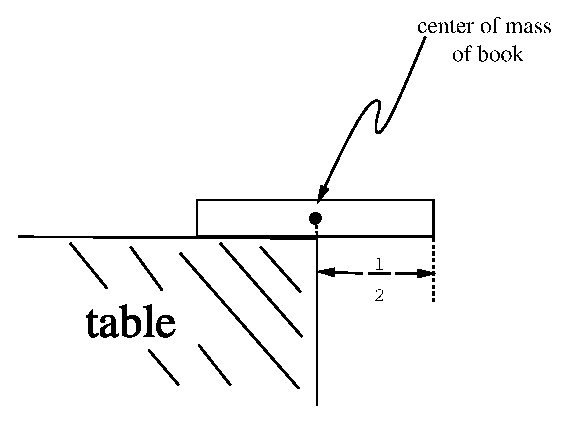
\includegraphics[width=.60\textwidth]{figures/drafts/bookstack-3}}
\caption{One book can overhang half a book length.}
\label{one-stable-book}
\end{figure}

Now suppose we have a stack of books that will not tip over if the
bottom book rests on the table---call that a \emph{stable stack}.
Let's define the \emph{overhang} of a stable stack to be the
horizontal distance from the center of mass of the stack to the
furthest edge of the top book.  So the overhang is purely a property
of the stack, regardless of its placement on the table.  If we place
the center of mass of the stable stack at the edge of the table as in
Figure~\ref{overhang}, the overhang is how far we can get the top book
in the stack to stick out past the edge.

\begin{figure}
\centerline{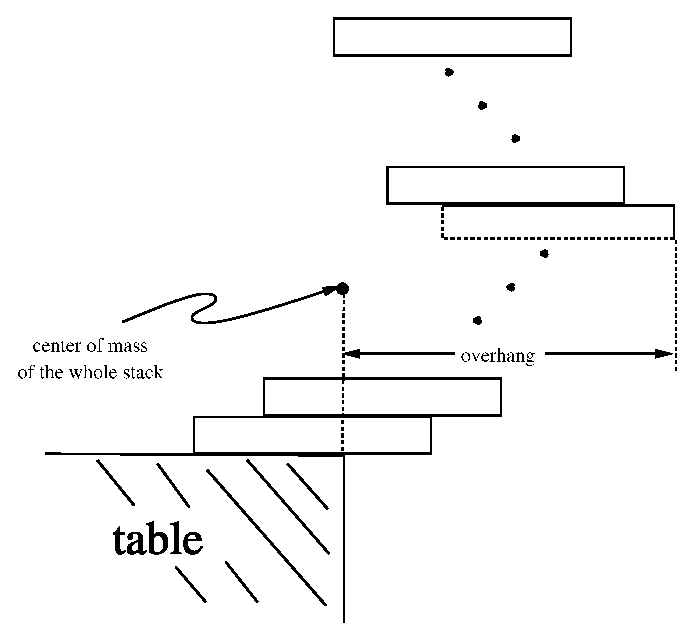
\includegraphics[width=.6\textwidth]{figures/drafts/bookstack-2}}
%\centerline{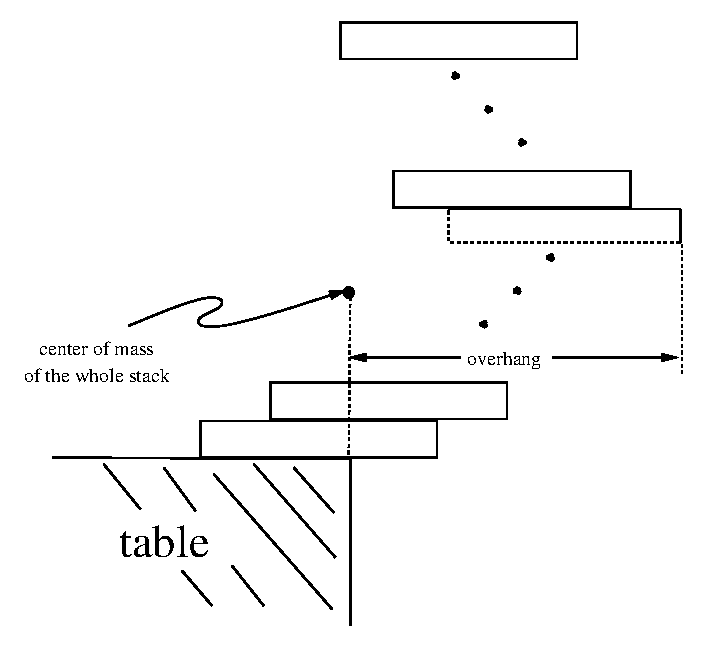
\psfig{file=figures/bookstack-2.ps,width=.4\textwidth}}
\caption{Overhanging the edge of the table.}
\label{overhang}
\end{figure}

In general, a stack of $n$~books will be stable if and only if the
center of mass of the top $i$~books sits over the $(i + 1)$st book
for $i = 1$, 2, \dots, $n - 1$.

So we want a formula for the maximum possible overhang $B_n$ achievable
with a stable stack of $n$~books.

We've already observed that the overhang of one book is~1/2 a book
length.  That is,
\[
    B_1 = \frac{1}{2}.
\]

Now suppose we have a stable stack of $n+1$ books with maximum overhang.
If the overhang of the $n$ books on top of the bottom book was not
maximum, we could get a book to stick out further by replacing the top
stack with a stack of $n$ books with larger overhang.  So the maximum
overhang $B_{n+1}$ of a stack of $n+1$ books is obtained by placing a
maximum overhang stable stack of $n$ books on top of the bottom book.  And
we get the biggest overhang for the stack of $n+1$ books by placing the
center of mass of the $n$ books right over the edge of the bottom book as
in Figure~\ref{Bn1}.

So we know where to place the $n+1$st book to get maximum overhang.
In fact, the reasoning above actually shows that this way of stacking
$n+1$ books is the \emph{unique} way to build a stable stack where the
top book extends as far as possible.  All we have to do is
calculate what this extension is.  

The simplest way to do that is to let the center of mass of the top
$n$ books be the origin.  That way the horizontal coordinate of the
center of mass of the whole stack of $n+1$ books will equal the
increase in the overhang.  But now the center of mass of the bottom
book has horizontal coordinate $1/2$, so the horizontal coordinate of
center of mass of the whole stack of $n+1$ books is
\[
\frac{0 \cdot n + (1/2) \cdot 1}{n+1} = \frac{1}{2(n +1)}.
\]

In other words, 
\begin{equation}\label{eqBn}
    B_{n+1} = B_n + \frac{1}{2(n+1)},
\end{equation}
as shown in Figure~\ref{Bn1}.

\begin{figure}
\centerline{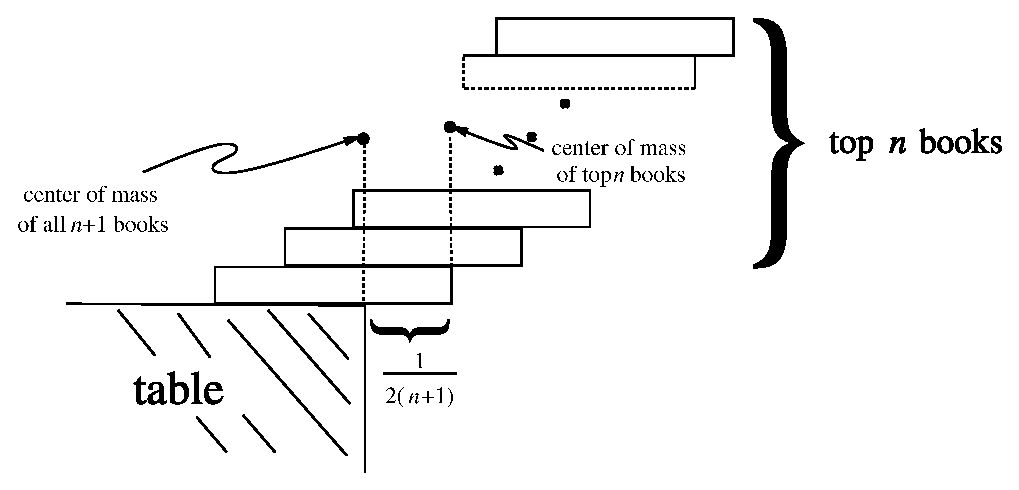
\includegraphics[width=.80\textwidth]{figures/drafts/bookstack-5}}
%\centerline{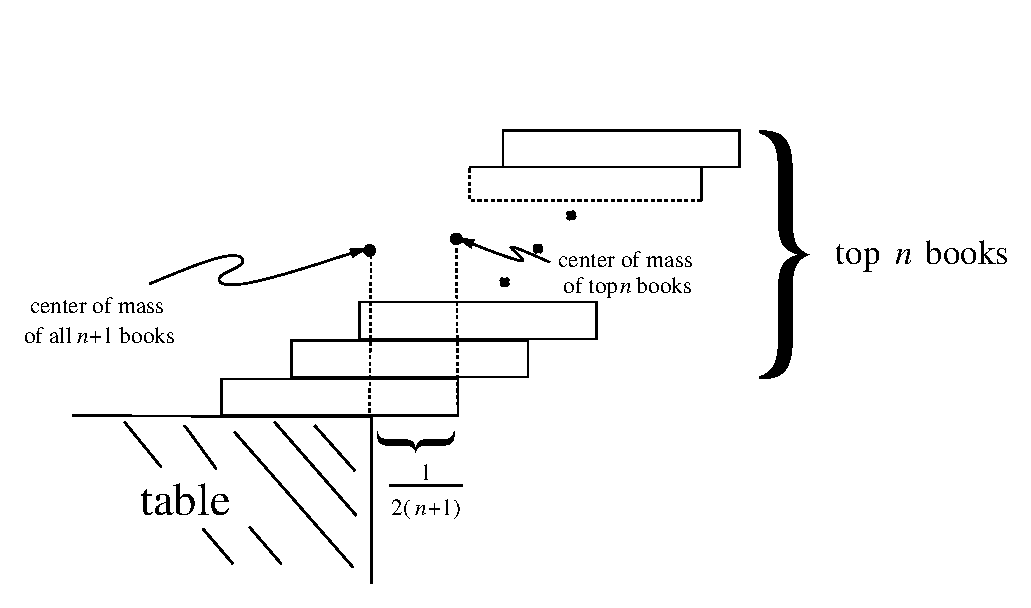
\psfig{file=figures/bookstack-5.ps,width=.80\textwidth}}
\caption{Additional overhang with $n+1$ books.}
\label{Bn1}
\end{figure}

Expanding equation~(\ref{eqBn}), we have
\begin{align}
B_{n+1} & = B_{n-1} + \frac{1}{2n} + \frac{1}{2(n+1)}\notag\\
        & = B_1 + \frac{1}{2 \cdot 2} + \cdots + \frac{1}{2n} +
            \frac{1}{2(n+1)}\notag\\
        & = \frac{1}{2}\sum_{i=1}^{n+1} \frac{1}{i}.\label{Bn+1sum}
\end{align}

So our next task is to examine the behavior of $B_n$ as $n$ grows.

\subsection{Harmonic Numbers}

\begin{definition}
The $n$th \term{harmonic number} $H_n$ is
\[
H_n \eqdef \sum_{i=1}^n \frac{1}{i}.
\]
\end{definition}
So~\eqref{Bn+1sum} means that
\[
B_n = \frac{H_n}{2}.
\]

The first few harmonic numbers are easy to compute.  For example, $H_4 = 1
+ \frac{1}{2} + \frac{1}{3} + \frac{1}{4} = \frac{25}{12} > 2$.  The fact that
$H_4$ is greater than 2 has special significance: it implies that the
total extension of a 4-book stack is greater than one full book!  This is
the situation shown in Figure~\ref{fig:optstack}.

\begin{figure}[htbp]
\centerline{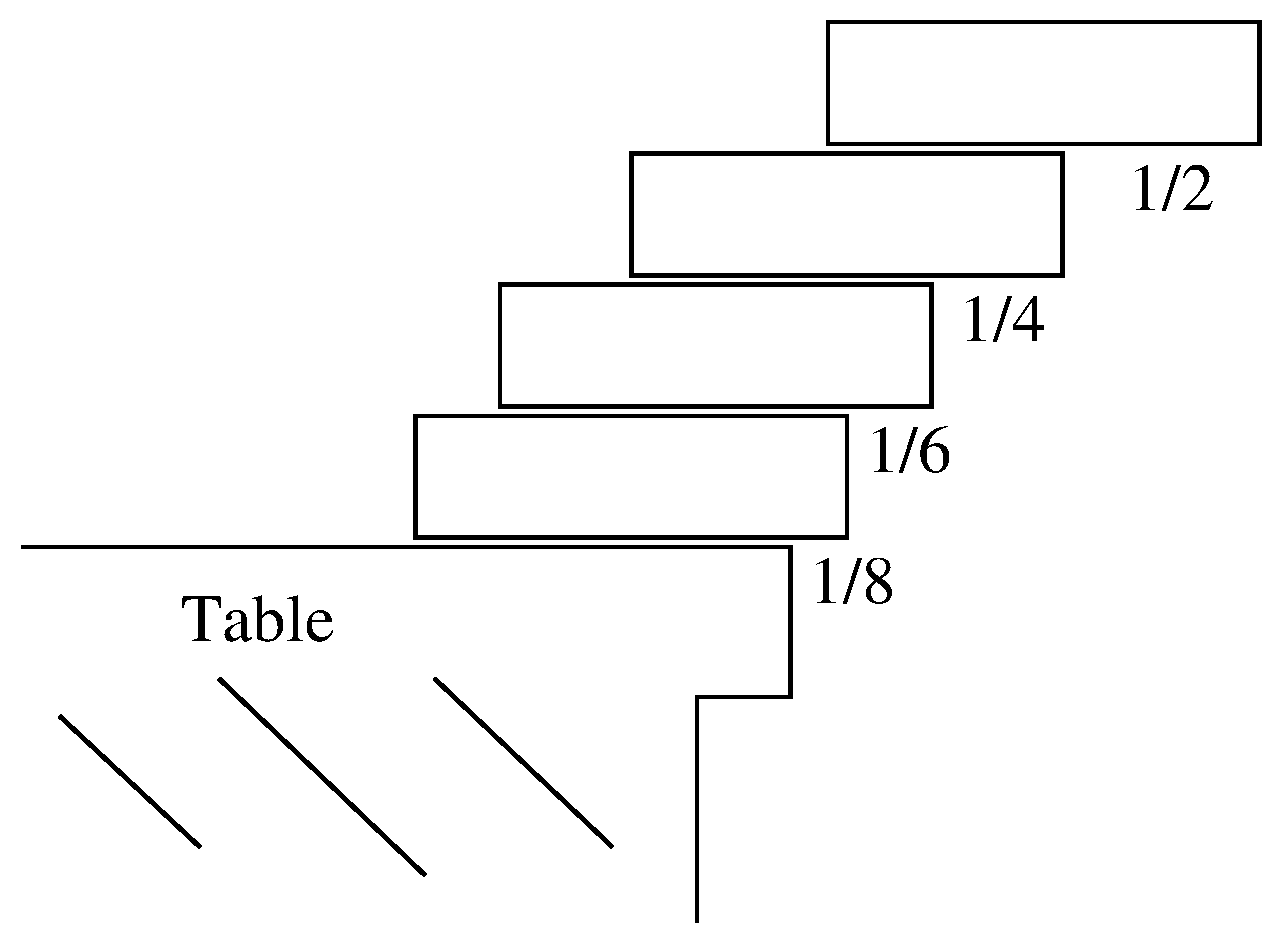
\includegraphics[height=1.5in]{figures/drafts/optstack}}
\caption{Stack of four books with maximum overhang.}
\label{fig:optstack}
\end{figure}

There is good news and bad news about harmonic numbers.  The bad news
is that there is no known closed-form expression for the harmonic
numbers.  The good news is that we can use
Theorem~\ref{weak_increasing_sum_bounds} to get close upper and lower
bounds on~$H_n$.  In particular, since
\begin{align*}
\int_1^n \frac{1}{x} \, dx
    = \ln(x) \; \Bigr|_1^n %\\
    = \ln(n),
\end{align*}
Theorem~\ref{weak_increasing_sum_bounds} means that
\begin{equation}\label{eqn:9G30}
    \ln(n) + \frac{1}{n} \le H_n \le \ln(n) + 1.
\end{equation}
In other words, the $n$th harmonic number is very close to~$\ln(n)$.

Because the harmonic numbers frequently arise in practice,
mathematicians have worked hard to get even better approximations for
them.  In fact, it is now known that
\begin{equation}\label{eqn:9K2}
    H_n = \ln(n) + \gamma + \frac{1}{2n} + \frac{1}{12n^2} +
        \frac{\epsilon(n)}{120n^4}
\end{equation}
Here $\gamma$ is a value $0.577215664\dots$ called \term{Euler's
  constant}, and $\epsilon(n)$ is between 0 and 1 for all $n$.  We
will not prove this formula.

We are now finally done with our analysis of the book stacking
problem.  Plugging the value of~$H_n$ into~\eqref{Bn+1sum}, we
find that the maximum overhang for $n$~books is very close
to~$\ln(n)/2$.  Since $\ln(n)$ grows to infinity as $n$~increases,
this means that if we are given enough books \begin{editingnotes}
(in theory anyway)
\end{editingnotes},
we can get a book to hang out arbitrarily far over the edge of the table.
Of course, the number of books we need will grow as an exponential
function of the overhang; it will take 227~books just to achieve an
overhang of~3, never mind an overhang of~100.

\subsubsection{Extending Further Past the End of the Table}
The overhang we analyzed above was the furthest out the \emph{top}
book could extend past the table.  This leaves open the question
of if there is some better way to build a stable stack where some book
other than the top stuck out furthest.  For example,
Figure~\ref{lab:bottom-book-furthest} shows a stable stack of two
books where the bottom book extends further out than the top book.
Moreover, the bottom book extends 3/4 of a book length past the end of
the table, which is the same as the maximum overhang for the top book
in a two book stack.

\begin{figure}
\subfloat[]{\graphic{Fig_G20-a}}
\qquad
\subfloat[]{\graphic{Fig_G20-b}}

\caption{Figure (a) shows a stable stack of two books where the
  bottom book extends the same amount past the end of the table as
  the maximum overhang two-book stack shown in Figure (b).}
\label{lab:bottom-book-furthest}
\end{figure}

Since the two book arrangement in
Figure~\ref{lab:bottom-book-furthest}(a) ties the maximum overhang
stack in Figure~\ref{lab:bottom-book-furthest}(b), we could take the
unique stable stack of $n$ books where the top book extends furthest,
and switch the top two books to look like
Figure~\ref{lab:bottom-book-furthest}(a).  This would give a stable
stack of $n$ books where the second from the top book extends the same
maximum overhang distance.  So for $n>1$, there are at least two ways
of building a stable stack of $n$ books which both extend the maximum
overhang distance---one way where the top book is furthest out, and
another way where the second from the top book is furthest out.

It is not too hard to prove that these are the \emph{only} two ways to
get a stable stack of books that achieves maximum overhang, providing
we stick to stacking only \emph{one} book on top of another.
\begin{editingnotes}
(see Problem~\ref{PS_optimal_overhang}).
\end{editingnotes}
But there is more to the story.  Building book piles with more than
one book resting on another---think of an inverted pyramid---it is
possible to get a stack of $n$ books to extend proportional to
$\sqrt[3]{n}$---much more than $\ln n$---book lengths without falling
over.  See~\cite{Paterson09},
\href{http://mathdl.maa.org/mathDL/22/?pa=content&sa=viewDocument&nodeId=3623&pf=1}
     {\emph{Maximum Overhang}}.


\subsection{Asymptotic Equality}\label{sec:asymptotic_equality}

For cases like equation~\ref{eqn:9K2} where we understand the growth
of a function like~$H_n$ up to some (unimportant) error terms, we use
a special notation,~$\sim$, to denote the leading term of the
function.  For example, we say that $H_n \sim \ln(n)$ to indicate that
the leading term of $H_n$ is $\ln(n)$.  More precisely:
\begin{definition}\label{def:sim}
  For functions $f,g: \reals \to \reals$, we say $f$ is%
\index{asymptotic notation!asymptotic equality|textbf}
\emph{asymptotically equal} to $g$, in symbols,
\[
f(x) \sim g(x)
\]
iff
\[
\lim_{x \rightarrow \infty} f(x)/g(x) = 1.
\]
\end{definition}

Although it is tempting to write $H_n \sim \ln(n) + \gamma$ to indicate
the two leading terms, this is not really right.  According to
Definition~\ref{def:sim}, $H_n \sim \ln(n) + c$ where $c$ is \emph{any
  constant}.  The correct way to indicate that $\gamma$ is the
second-largest term is $H_n - \ln(n) \sim \gamma$.

The reason that the $\sim$ notation is useful is that often we do not care
about lower order terms.  For example, if $n = 100$, then we can compute
$H(n)$ to great precision using only the two leading terms:
\[
\abs{H_n - \ln(n) - \gamma} \leq \abs{\frac{1}{200} - \frac{1}{120000} +
\frac{1}{120 \cdot 100^4}} < \frac{1}{200}.
\]

We will spend a lot more time talking about asymptotic notation at the
end of the chapter.  But for now, let's get back to using sums.

\begin{problems}
\classproblems
\pinput{CP_holy_grail}
\pinput{CP_harmonic_number_divergence}
\pinput{CP_conditional_convergence}

\homeworkproblems
\pinput{PS_bug_on_rug_harmonic_number}
\pinput{PS_alt_harmonic_converges}

\begin{editingnotes}
\pinput{PS_optimal_overhang}
\end{editingnotes}

\examproblems
\pinput{MQ_Summation}

\end{problems}

\section{Products}\label{sec:closed_products}

We've covered several techniques for finding closed forms for sums but
no methods for dealing with products.  Fortunately, we do not need to
develop an entirely new set of tools when we encounter a product such
as
\begin{equation}\label{eqn:9P1}
    n! \eqdef \prod_{i = 1}^n i.
\end{equation}
That's because we can convert any product into a sum by taking a
logarithm.  For example, if
\[
    P = \prod_{i  = 1}^n f(i),
\]
then
\[
    \ln(P) = \sum_{i = 1}^n \ln(f(i)).
\]
We can then apply our summing tools to find a closed form (or
approximate closed form) for~$\ln(P)$ and then exponentiate at the end
to undo the logarithm.

For example, let's see how this works for the \idx{factorial}
function~$n!$.  We start by taking the logarithm:
\begin{align*}
\ln (n!)
       & =  \ln(1 \cdot 2 \cdot 3 \cdots (n-1) \cdot n) \\
       & =  \ln(1) + \ln(2) + \ln(3) + \cdots + \ln(n-1) + \ln(n) \\
       & =  \sum_{i=1}^n \ln(i).
\end{align*}

Unfortunately, no closed form for this sum is known.  However, we can
apply Theorem~\ref{weak_increasing_sum_bounds} to find good
closed-form bounds on the sum.  To do this, we first compute
\begin{align*}
\int_1^n \ln(x) \, dx
    &= x \ln(x) - x \Bigr|_1^n \\
    &= n \ln(n) - n + 1.
\end{align*}
Plugging into Theorem~\ref{weak_increasing_sum_bounds}, this means that
\[
    n \ln(n) - n + 1
    \;\le\; \sum_{i = 1}^n \ln(i)
    \;\le\; n \ln(n) - n + 1 + \ln(n).
\]
Exponentiating then gives
\begin{equation}\label{eqn:9Q1}
    \frac{n^n}{e^{n - 1}} \;\le\; n! \;\le\; \frac{n^{n + 1}}{e^{n - 1}}.
\end{equation}
This means that $n!$ is within a factor of~$n$ of~$n^n/e^{n - 1}$.

\subsection{Stirling's Formula}

The most commonly used product in discrete
mathematics is probably $n!$, and mathematicians have workedto find tight
closed-form bounds on its value.  The most useful bounds are
given in Theorem~\ref{thm:stirling}.

\begin{theorem}[\term{Stirling's Formula}]\label{thm:stirling}
For all $n \ge 1$,
\[
    n! = \stirling{n}{e^{\epsilon(n)}}
%\sqrt{2 \pi n} \paren{\frac{n}{e}}^n e^{\epsilon(n)}
\]
where
\[
    \frac{1}{12 n + 1} \le \epsilon(n) \le \frac{1}{12n}.
\]
\end{theorem}

Theorem~\ref{thm:stirling} can be proved by induction (with some pain),
and there are lots of proofs using elementary
calculus,
\iffalse
but the details are a bit painful (even for us) and so
\fi
but we won't go into them.

There are several important things to notice about Stirling's
Formula.  First, $\epsilon(n)$ is always positive.  This means that
\begin{equation}\label{eqn:9ZA}
    n! > \stirling{n}
%\sqrt{2\pi n} \paren{\frac{n}{e}}^n
\end{equation}
for all~$n \in \nngint^+$.

Second, $\epsilon(n)$~tends to zero as $n$~gets large.  This means
that
\begin{equation}\label{nfacsim}%\label{eqn:9.28}
    n! \sim \stirling{n}
%\sqrt{2\pi n} \paren{\frac{n}{e}}^n,
\end{equation}
which is impressive.  After all, who would expect both $\pi$ and~$e$ to
show up in a closed-form expression that is asymptotically equal to~$n!$?

Third, $\epsilon(n)$~is small even for small values of~$n$.  This
means that Stirling's Formula provides good approximations for~$n!$
for most all values of~$n$.  For example, if we use
\[
    \stirling{n}
\]
as the approximation for~$n!$, as many people do, we are guaranteed
to be within a factor of
\[
    e^{\epsilon(n)} \le e^{\frac{1}{12n}}
\]
of the correct value.  For $n \ge 10$, this means we will be
within~1\% of the correct value.  For~$n \ge 100$, the error will be
less than~0.1\%.

If we need an even closer approximation for~$n!$, then we could use
either
\[
    \stirling{n} e^{1/12n}
\]
or
\[
    \stirling{n} e^{1/(12n + 1)}
\]
depending on whether we want an upper, or a lower, bound.  By
Theorem~\ref{thm:stirling}, we know that both bounds will be within a
factor of
\[
    e^{ \frac{1}{12n} - \frac{1}{12n + 1} } = e^{\frac{1}{144n^2 + 12n }}
\]
of the correct value.  For~$n \ge 10$, this means that either bound
will be within~0.01\% of the correct value.  For~$n \ge 100$, the
error will be less than~0.0001\%.

For quick future reference, these facts are summarized in
Corollary~\ref{cor:9A2} and Table~\ref{fig:9A1}.

\begin{table}\redrawntrue

\renewcommand{\arraystretch}{1.5}

\begin{tabular}{l|llll}

\multicolumn{1}{l}{\emph{Approximation}}
    & $n \ge 1$
    & $n \ge 10$
    & $n \ge 100$
    & $n \ge 1000$ \\
\cline{2-5}
$\stirling{n}$
    & ${}<{}$10\%
    & ${}<{}$1\%
    & ${}<{}$0.1\%
    & ${}<{}$0.01\%\\

$\stirling{n} e^{1/12n}$
    & ${}<{}$1\%
    & ${}<{}$0.01\%
    & ${}<{}$0.0001\%
    & ${}<{}$0.000001\%
\end{tabular}

\caption{Error bounds on common approximations for~$n!$ from
  Theorem~\ref{thm:stirling}.  For example, if~$n \ge 100$, then
  $\protect\stirling{n}$ approximates~$n!$ to within~0.1\%.}

\label{fig:9A1}

\end{table}

\begin{corollary}\label{cor:9A2}
\begin{align*}
n! < \stirling{n} \cdot
 \begin{cases}
1.09 & \text{ for }   n \ge 1,\\
1.009 & \text{ for }  n \ge 10,\\
1.0009 & \text{ for } n \ge 100.
\end{cases}
\end{align*}

\iffalse

For $n \ge 1$,
\[
    n! < 1.09 \stirling{n}.
\]
For $n \ge 10$,
\[
    n! < 1.009 \stirling{n}.
\]
For $n \ge 100$,
\[
    n! < 1.0009 \stirling{n}.
\]
\fi

\end{corollary}

\begin{editingnotes}
MOVE INTO AN EXERCISE:
\end{editingnotes}

\section{Double Trouble}\label{doublesum_sec}

Sometimes we have to evaluate sums of sums, otherwise known as
\term{double summations}.  This sounds hairy, and sometimes it is.
But usually, it is straightforward---you just evaluate the inner sum,
replace it with a closed form, and then evaluate the outer sum (which
no longer has a summation inside it).  For example,\footnote{OK, so
  maybe this one is a little hairy, but it is also fairly
  straightforward.  Wait till you see the next one!}
\begingroup
\openup3pt
\begin{align*}
\sum_{n=0}^{\infty} \paren{y^n \sum_{i=0}^n x^i}
 & = \sum_{n=0}^{\infty} \paren{y^n \frac{1-x^{n+1}}{1-x}}
     & \text{equation~\ref{geometric-sum-n}}\\
%
 & = \paren{\frac{1}{1-x}} \sum_{n=0}^{\infty} y^n
     - \paren{\frac{1}{1-x}} \sum_{n=0}^{\infty} y^nx^{n+1} \\
%
 & = \frac{1}{(1-x)(1-y)}
    - \paren{\frac{x}{1 - x}} \sum_{n=0}^{\infty} \paren{xy}^n
      & \text{Theorem~\ref{th:series}}\\
%
 & = \frac{1}{(1-x)(1-y)} - \frac{x}{(1-x)(1-xy)}
      & \text{Theorem~\ref{th:series}}\\
%
  & = \frac{\paren{1-xy} - x(1-y)}{(1-x)(1-y)(1-xy)}\\
%
  & = \frac{1-x}{(1-x)(1-y)(1-xy)}\\
%
  & = \frac{1}{(1-y)(1-xy)}.
\end{align*}
\endgroup

When there's no obvious closed form for the inner sum, a special trick
that is often useful is to try \emph{exchanging the order of
  summation.}  For example, suppose we want to compute the sum of the
first $n$~\idx{harmonic numbers}
\begin{equation}\label{eqn:9B}
    \sum_{k=1}^n H_k = \sum_{k=1}^n \sum_{j=1}^k \frac{1}{j}
\end{equation}
For intuition about this sum, we can apply Theorem~\ref{weak_increasing_sum_bounds} to
equation~\ref{eqn:9G30} to conclude that the sum is close to
\begin{align*}
\int_{1}^n \ln(x) \, dx
    =  x \ln(x) - x \; \Bigr|_1^n %\\
    = n \ln(n) - n + 1.
\end{align*}

Now let's look for an exact answer.  If we think about the pairs
$(k,j)$ over which we are summing, they form a triangle:
\[
\begin{array}{cc|ccccccc}
 &  & j &   &   &   &   &       &   \\
 &  & 1 & 2 & 3 & 4 & 5 & \dots & n \\
\hline
k & 1 & 1\\
  & 2 &1&1/2\\
  & 3 &1&1/2&1/3\\
  & 4 &1&1/2&1/3&1/4\\
  &   &\dots\\
  & n &1&1/2&&\dots&&&1/n
\end{array}
\]
The summation in equation~\ref{eqn:9B} is summing each row and then
adding the row sums.  Instead, we can sum the columns and then add the
column sums.  Inspecting the table we see that this double sum can be
written as
\begingroup
\openup3pt
\begin{align}
\sum_{k=1}^n H_k &= \sum_{k=1}^n \sum_{j=1}^k \frac{1}{j}\notag\\
&= \sum_{j=1}^n \sum_{k=j}^n \frac{1}{j}\notag\\
&= \sum_{j=1}^n \frac{1}{j} \sum_{k=j}^n 1\notag\\
&= \sum_{j=1}^n \frac1j (n-j+1)\notag\\
&= \sum_{j=1}^n \frac{n+1}j - \sum_{j=1}^n \frac{j}{j}\notag\\
&= (n+1)\sum_{j=1}^n \frac1j - \sum_{j=1}^n 1\notag\\
&= (n+1)H_n-n.\label{sHk}
\end{align}
\endgroup


\section{Asymptotic Notation}\label{asymptotic_sec}
\index{asymptotic notation|textbf}

Asymptotic notation is a shorthand used to give a quick measure of the
behavior of a function $f(n)$ as $n$ grows large.  For example, the
asymptotic notation~\idx{$\sim$} of Definition~\ref{def:sim} is a
binary relation indicating that two functions grow at the \emph{same}
rate.  There is also a binary relation ``little oh'' indicating that
one function grows at a significantly \emph{slower} rate than another
and ``Big Oh'' indicating that one function grows not much more
rapidly than another.

\subsection{Little Oh}
\index{o@o (little o)|see{asymptotic notation}}
\index{little o|see{asymptotic notation}}

\begin{definition}
  For functions $f,g: \reals \to \reals$, with $g$ nonnegative, we say
  $f$ is%
\index{asymptotic notation!asymptotically smaller, o, little o|textbf} 
\emph{asymptotically
    smaller} than~$g$, in symbols,
\[
f(x) = o(g(x)),
\]
iff
\[
\lim_{x \rightarrow \infty} f(x)/g(x) = 0.
\]
\end{definition}

For example, $1000x^{1.9} = o(x^2)$ because
\[
\lim_{x \rightarrow \infty} \frac{1000x^{1.9}}{x^2}
  = 1000\lim_{x \rightarrow \infty} \frac{1}{x^{0.1}}
     = 1000\cdot 0 = 0.
\]
This argument generalizes directly to yield
\begin{lemma}\label{xaoxb}
\begin{align}
f = o(g) & \QIMPLIES  c\cdot f = o(g) & \text{for any constant $c$}.\label{fogcf}\\
x^a & = o(x^b) & \text{for constants $0\leq a<b$}. \label{xaoxbeq}
\end{align}
\end{lemma}

Also, log's grow more slowly than roots:
%Using the familiar fact that  $\log x < x$ for all $x >1$, we can prove
\begin{lemma}\label{logxxe}
$\log_a x = o(x^{\epsilon})$ for all $a>1, \epsilon >0$.
\end{lemma}

\begin{proof}
For $y \geq 1$, we have $1/y \leq y$.  Taking integrals from 1 to $z$,
we conclude
\begin{equation}\label{lnz<z2}
\ln z \leq \frac{z^2}{2}
\end{equation}
for $z \geq 1$.  Choose $\epsilon > \delta > 0$ and let $z =
\sqrt{x^\delta}$ in~\eqref{lnz<z2}.  Then
\begin{align}
\frac{\delta \ln x}{2} &\leq  \frac{x^{\delta}}{2},\notag\\
\ln x  & \leq \frac{x^{\delta}}{\delta} = o(x^{\epsilon}) & \text{by Lemma~\ref{xaoxb}}\label{lnxfxd}.
\end{align}
Finally, for any real number $a>1$,
\[
\log_a x = \frac{\ln x}{\ln a} = o(x^{\epsilon})
\]
by~\eqref{lnxfxd} and \eqref{fogcf}.
\end{proof}

\begin{corollary}\label{xbax}
$x^b = o(a^x)$ for any $a,b \in \reals$ with $a>1$.
\end{corollary}

Lemma~\ref{logxxe} and Corollary~\ref{xbax} can also be proved using
l'H\^opital's Rule or the Maclaurin Series for $\log x$ and $e^x$.
Proofs can be found in most calculus texts.

\subsection{Big Oh}
\index{O@O (big O)|see{asymptotic notation}}
\index{big O|see{asymptotic notation}}
\index{asymptotic notation!big O|textbf}

``Big Oh'' is the most frequently used asymptotic notation.  It is used to
give an upper bound on the growth of a function, such as the running
time of an algorithm.  There is a standard definition of Big Oh given
below in~\ref{def:O}, but we'll begin with an alternative definition
that makes several basic properties of Big Oh more apparent.

\begin{definition}\label{def:Olimsup}
Given functions $f, g : \reals \to \reals$ with $g$ nonnegative, we
say that
\[
f = O(g)
\]
iff
\[
\limsup_{x \rightarrow \infty} \abs{f(x)}/g(x) < \infty.
\]
\end{definition}
Here we're using the technical notion of \term{limit
  superior}\footnote{The precise definition of $\limsup$ is
\[
\limsup_{x \rightarrow \infty} h(x) \eqdef \lim_{x \rightarrow \infty}
\text{lub}_{y \geq x} h(y),
\]
where ``lub'' abbreviates ``least upper bound.''} instead of just
limit.  But because limits and lim sup's are the same when limits
exist, this formulation makes it easy to check basic properties of Big
Oh.  We'll take the following Lemma for granted.
\begin{lemma}\label{limimpsup}
If a function $f: \reals \to \reals$ has a finite or infinite limit as
its argument approaches infinity, then its limit and limit superior
are the same.
\iffalse
\[
\lim_{x \rightarrow \infty} f(x) < \infty\ \QIMP\ \limsup_{x
  \rightarrow \infty} f(x) = \lim_{x \rightarrow \infty} f(x).
\fi
\end{lemma}
  
Now Definition~\ref{def:Olimsup} immediately implies:
\begin{lemma}\label{osimO}
If $f = o(g)$ or $f \sim g$, then $f = O(g)$.
\end{lemma}

\begin{proof}
$\lim f/g=0$ or $\lim f/g=1$ implies $\lim f/g<\infty$, so by
  Lemma~\ref{limimpsup}, $\limsup f/g<\infty$.
\end{proof}
Note that the converse of Lemma~\ref{osimO} is not true.  For example,
$2x = O(x)$, but $2x \not\sim x$ and $2x \neq o(x)$.

We also have:
\begin{lemma}
If $f = o(g)$, then it is \emph{not} true that $g = O(f)$.
\end{lemma}

\begin{proof}
\[
\lim_{x \rightarrow \infty} \frac{g(x)}{f(x)} =
 \frac{1}{\lim_{x \rightarrow \infty} f(x)/g(x)} =
 \frac{1}{0} = \infty,
\]
so by Lemma~\ref{limimpsup}, %$\limsup_{x \rightarrow \infty} \frac{g(x)}{f(x)} = \infty$ 
$g \neq O(f)$.
\end{proof}

We need lim sup's in Definition~\ref{def:Olimsup} to cover cases when
limits don't exist.  For example, if $f(x)/g(x)$ oscillates between 3
and 5 as $x$ grows, then $\lim_{x \rightarrow \infty} f(x)/g(x)$ does
not exist, but $f = O(g)$ because $\limsup_{x \rightarrow \infty}
f(x)/g(x) = 5$.

An equivalent, more usual formulation of big O does not mention $\limsup$'s:
\begin{definition}\label{def:O}
Given functions $f, g : \reals \to \reals$ with $g$
nonnegative, we say
\[
f = O(g)
\]
iff there exists a constant $c \geq 0$ and an $x_0$ such that for all
$x \geq x_0$, $\abs{f(x)} \leq c g(x)$.
\end{definition}

This definition is rather complicated, but the idea is simple: $f(x) =
O(g(x))$ means $f(x)$ is less than or equal to $g(x)$, except that
we're willing to ignore a constant factor, namely $c$, and to allow
exceptions for small $x$, namely, for $x < x_0$.  So in the case that
$f(x)/g(x)$ oscillates between 3 and 5, $f=O(g)$ according to
  Definition~\ref{def:O} because $f \leq 5g$.

\begin{proposition}
$100x^2 = O(x^2)$.
\end{proposition}

\begin{proof}
Choose $c = 100$ and $x_0 = 1$.  Then the proposition holds, since for all
$x \geq 1$, $\abs{100x^2} \leq 100 x^2$.
\end{proof}

\begin{proposition}\label{x2O}
$x^2 + 100x + 10 = O(x^2)$.
\end{proposition}

\begin{proof}
$(x^2 + 100x + 10)/x^2 = 1 + 100/x + 10/x^2$ and so its limit as $x$
approaches infinity is $1 + 0 + 0 = 1$.  So in fact, $x^2 + 100x + 10 \sim
x^2$, and therefore $x^2 + 100x + 10 = O(x^2)$.  Indeed, it's conversely
true that $x^2= O(x^2 + 100x + 10)$.
\end{proof}

Proposition~\ref{x2O} generalizes to an arbitrary polynomial:
\begin{proposition}
    $a_k x^k + a_{k-1} x^{k-1} + \cdots + a_1x + a_0 = O(x^k)$.
\end{proposition}
We'll omit the routine proof.

Big Oh notation is especially useful when describing the running time
of an algorithm.  For example, the usual algorithm for multiplying $n
\times n$ matrices uses a number of operations proportional to~$n^3$
in the worst case.  This fact can be expressed concisely by saying
that the running time is $O(n^3)$.  The asymptotic notation highlights
the behavior of the algorithm at a high level that abstracts away
implementations details that may be programming language or
machine-specific.

It turns out that there is another \idx{matrix multiplication}
procedure that uses $O(n^{2.55})$ operations.\footnote{It is
  conceivable that there is an $O(n^2)$ matrix multiplication
  procedure, but none is known.}  This is an asymptotically faster
procedure, and it will definitely be much faster on large enough
matrices.  But being asymptotically faster does not mean that it is a
better choice.  In fact, the $O(n^{2.55})$-operation multiplication
procedure is almost never used in practice because it only becomes
relatively efficient on matrices of impractical size.

However, the fact that the $O(n^{2.55})$ procedure is asymptotically
faster indicates that it involves \emph{new ideas} that go beyond
optimized implementations of the $O(n^3)$ method.  We can expect that
these new ideas can lead to practical matrix multiplication procedures
that are significantly faster than the usual ones.

\begin{editingnotes}
Check up latest info on matrix multiplication packages.  Maybe add a
problem introducing Strassen's method.
\end{editingnotes}

\subsection{\index{$\Theta()$}Theta}

Sometimes we want to specify that a running time~$T(n)$ is precisely
quadratic up to constant factors (both upper bound \emph{and} lower
bound).  We could do this by saying that $T(n) = O(n^2)$ and $n^2 =
O(T(n))$, but rather than say both, mathematicians have devised yet
another symbol $\Theta$ to do the job.

\begin{definition}\label{def:Theta}
\[
    f = \Theta(g)
    \qiff
    f=O(g) \text{ and } g=O(f).
\]
\end{definition}

The statement $f = \Theta(g)$ can be paraphrased intuitively as
``$f$ and $g$ are equal to within a constant factor.''

\iffalse
Indeed, by
Theorem~\ref{thm:9S2}, we know that
\[
    f = \Theta(g) \qiff \text{$f = O(g)$ and $f = \Omega(g)$}.
\]
\fi

The Theta notation allows us to highlight growth rates and suppress
distracting factors and low-order terms.  For example, if the running
time of an algorithm is
\[
T(n) = 10n^3 - 20n^2 + 1,
\]
then we can more simply write
\[
T(n) = \Theta(n^3).
\]
In this case, we would say that \emph{$T$ is of order $n^3$} or that
\emph{$T(n)$ grows cubically}, which is often the main thing we really
want to know.  Another such example is
\[
{{\pi^23^{x-7} + \frac{(2.7x^{113} + x^9- 86)^4}{\sqrt{x}} - 1.08^{3x}}} =
\Theta(3^x).
\]

Just knowing that the running time of an algorithm is $\Theta(n^3)$,
for example, is useful, because if $n$ doubles we can predict that the
running time will \emph{by and large}\footnote{Since $\Theta(n^3)$
  only implies that the running time $T(n)$ is between $cn^3$ and
  $dn^3$ for constants $0<c<d$, the time $T(2n)$ could regularly
  exceed $T(n)$ by a factor as large as $8d/c$.  The factor is sure to
  be close to 8 for all large $n$ only if $T(n) \sim n^3$.} increase
by a factor of at most $8$ for large $n$.  In this way, Theta notation
preserves information about the scalability of an algorithm or system.
Scalability is, of course, a big issue in the design of algorithms and
systems.


\subsection{Pitfalls with Asymptotic Notation}

There is a long list of ways to make mistakes with asymptotic
notation.  This section presents some of the ways that big O notation
can lead to trouble.  With minimal effort, you can cause just
as much chaos with the other symbols.

\begin{editingnotes}
\subsection*{Pitfalls with Asymptotic Notation and Induction}
%From FTL's Akra-Bazzi section

We've seen that asymptotic notation is quite useful, particularly in
connection with recurrences.  And induction is our favorite proof
technique.  But mixing the two  is risky business; there is great
potential for subtle errors and false conclusions!

\begin{falseclm*}
If
\begin{align*}
   T(1)   &= 1 & \text{and}\\
   T(n)   &= 2 T(n/2) + n,
\end{align*}
then $T(n) = O(n)$.
\end{falseclm*}

The Akra-Bazzi theorem implies that the correct solution is $T(n) =
\Theta(n \log n)$ and so this claim is false.  But where does the
following ``proof'' go astray?

\begin{bogusproof}
The proof is by strong induction.  Let $P(n)$ be the proposition that
$T(n) = O(n)$.

\inductioncase{Base case}: $P(1)$ is true because $T(1) = 1 = O(1)$.

\inductioncase{Inductive step}:
For $n \ge 2$, assume $P(1), P(2), \dots, P(n - 1)$ to
prove~$P(n)$.  We have
\begin{align*}
   T(n) &= 2 \cdot T(n/2) + n \\
        &= 2 \cdot O(n/2) + n \\
        &= O(n).
\end{align*}
The first equation is the recurrence, the second uses the assumption
$P(n/2)$, and the third is a simplification.
\end{bogusproof}

Where's the bug?  The proof is already far off the mark in the second
sentence, which defines the induction hypothesis.  The statement
``$T(n) = O(n)$'' is either true or false; it's validity does not
depend on a particular value of~$n$.  Thus the very idea of trying to
prove that the statement holds for $n = 1, 2, \dots$, is
wrong-headed.

The safe way to reason inductively about asymptotic phenomena is to
\emph{work directly with the definition of the asymptotic notation}.  Let's try
to prove the claim above in this way.  Remember that $f(n) = O(n)$
means that there exist constants $n_0$ and~$c > 0$ such that
$\abs{f(n)} \le cn$ for all~$n \ge n_0$.  (Let's not worry about the
absolute value for now.)  If all goes well, the proof attempt should
fail in some blatantly obvious way, instead of in a subtle,
hard-to-detect way like the earlier argument.  Since our perverse goal
is to demonstrate that the proof won't work for \emph{any} constants
$n_0$ and~$c$, we'll leave these as variables and assume only that
they're chosen so that the base case holds; that is, $T(n_0) \le cn$.

\begin{proof}[Proof Attempt]
We use strong induction.  Let $P(n)$ be the proposition that $T(n) \le
cn$.

\inductioncase{Base case}:
$P(n_0)$ is true, because $T(n_0) \le cn$.

\inductioncase{Inductive step}:
For $n > n_0$, assume that $P(n_0)$, \dots, $P(n - 1)$ are true in
order to prove~$P(n)$.  We reason as follows:
\begin{align*}
T(n)   &=  2 T(n/2) + n \\
      &\le 2 c(n/2) + n \\
      &=  cn + n \\
      &=  (c + 1) n \\
      &\nleq c n.  \qedhere
\end{align*}
\end{proof}

The first equation is the recurrence.  Then we use induction and
simplify until the argument collapses!

In general, it is a good idea to stay away from asymptotic notation
altogether while you are doing the induction.  Once the induction is
over and done with, then you can safely use big O to simplify your
result.
\end{editingnotes}

\subsubsection{The Exponential Fiasco}

Sometimes relationships involving big O are not so obvious.  For
example, one might guess that $4^x = O(2^x)$ since 4 is only a
constant factor larger than 2.  This reasoning is incorrect, however;
$4^x$ actually grows as the square of~$2^x$.

\subsubsection{Constant Confusion}

Every constant is $O(1)$.  For example, $17 = O(1)$.  This is true because
if we let $f(x) = 17$ and $g(x) = 1$, then there exists a $c > 0$ and an
$x_0$ such that $\abs{f(x)} \leq c g(x)$.  In particular, we could choose
$c$ = 17 and $x_0 = 1$, since $\abs{17} \leq 17 \cdot 1$ for all $x \geq
1$.  We can construct a false theorem that exploits this fact.

\begin{falsethm}
\[
\sum_{i=1}^n i = O(n)
\]
\end{falsethm}

\begin{bogusproof}
Define $f(n) = \sum_{i=1}^n i = 1 + 2 + 3 + \cdots + n$.  Since we
have shown that every constant $i$ is $O(1)$, $f(n) = O(1) + O(1) +
\cdots + O(1) = O(n)$.
\end{bogusproof}

Of course in reality $\sum_{i=1}^n i = n(n+1)/2 \neq O(n)$.

The error stems from confusion over what is meant in the statement $i
= O(1)$.  For any \emph{constant} $i\in \nngint$ it is true that $i
= O(1)$.  More precisely, if $f$ is any constant function, then $f =
O(1)$.  But in this False Theorem, $i$ is not constant---it ranges
over a set of values $0, 1,\dots, n$ that depends on~$n$.

And anyway, we should not be adding $O(1)$'s as though they were numbers.
We never even defined what $O(g)$ means by itself; it should only be used
in the context ``$f = O(g)$'' to describe a relation between functions $f$
and $g$.

\subsubsection{Equality Blunder}

The notation $f = O(g)$ is too firmly entrenched to avoid, but the use of
``='' is regrettable.  For example, if $f = O(g)$, it seems quite
reasonable to write $O(g) = f$.  But doing so might tempt us to the
following blunder: because $2n = O(n)$, we can say $O(n) = 2n$.  But $n =
O(n)$, so we conclude that $n = O(n) = 2n$, and therefore $n = 2n$.  To
avoid such nonsense, we will never write ``$O(f) = g$.''

Similarly, you will often see statements like
\[
    H_n = \ln(n) + \gamma + O\paren{\frac{1}{n}}
\]
or
\[
    n! = (1 + o(1)) \stirling{n}
%\sqrt{2\pi n} \paren{\frac{n}{e}}^n.
\]
In such cases, the true meaning is
\[
    H_n = \ln(n) + \gamma + f(n)
\]
for some~$f(n)$ where $f(n) = O(1/n)$, and
\[
    n! = (1 + g(n)) \stirling{n}
%\sqrt{2\pi n} \paren{\frac{n}{e}}^n
\]
where $g(n) = o(1)$.  These last transgressions are OK as long as you
(and your reader) know what you mean.

\subsubsection{Operator Application Blunder}

It's tempting to assume that familiar operations preserve asymptotic
relations, but it ain't necessarily so.  For example, $f\sim g$ in
general does not even imply that $3^f = \Theta\paren{3^g}$.  On the other hand,
some operations preserve and even strengthen asymptotic relations, for
example,
\[
f = \Theta(g)\ \QIMPLIES\ \ln f \sim \ln g.
\]
See Problem~\ref{PS_Stirlings_and_log_n_factorial}.

\subsection{\index{$\Omega$@big omega}Omega (Optional)}\label{omega_subsec}

Sometimes people incorrectly use Big Oh in the context of a lower
bound.  For example, they might say, ``The running time $T(n)$ is at
least $O(n^2)$.''  This is another blunder!  Big Oh can only be used
for \emph{upper} bounds.  The proper way to express the lower bound
would be
\[
n^2 = O(T(n)).
\]
The lower bound can also be described with another special notation
``big Omega\index{asymptotic notation!big Omega|textbf}.''
\begin{definition}\label{def:Omega}
Given functions $f, g : \reals \to \reals$ with $f$~nonnegative,
define
\[
    f = \Omega(g)
\]
to mean
\[
g = O(f).
\]
\end{definition}
For example, $x^2 = \Omega(x)$, \ $2^x = \Omega(x^2)$ and $x/100 =
\Omega(100 x + \sqrt{x})$.

So if the running time of your algorithm on inputs of size~$n$
is~$T(n)$, and you want to say it is at least quadratic, say
\[
    T(n) = \Omega(n^2).
\]

There is a similar ``little \index{asymptotic notation!little
  omega|textbf} omega'' notation for lower bounds corresponding to
little o:

\begin{definition}\label{def:omega}
For functions $f, g: \reals \to \reals$ with $f$~nonnegative, define
\[
    f = \omega(g)
\]
to mean
\[
g = o(f).
\]
\end{definition}

For example, $x^{1.5} = \omega(x)$ and $\sqrt{x} = \omega(\ln^2(x))$.

The little omega symbol is not as widely used as the other asymptotic
symbols we defined.

\begin{problems}
\practiceproblems
\pinput{TP_Practice_with_Big_O}
\pinput{MQ_asymptotics_table}
\pinput{MQ_asymptotic_true_false}
\pinput{MQ_stirlings_asymptotics}
\pinput{TP_Stirlings_Formula}
\pinput{TP_limsup}

\homeworkproblems
\pinput{PS_little_oh_properties_arm}
\pinput{PS_asymptotics_table}
\pinput{PS_asymptotics_ordering}
\pinput{PS_Stirlings_and_log_n_factorial}
\pinput{PS_asymptotics_and_stirlings}
\pinput{PS_asymptotics_pairs}
\pinput{PS_sum_of_sixth_powers}


\classproblems
\pinput{CP_Theta_log_n_factorial}
\pinput{CP_asymptotic_equality_properties}
\pinput{CP_big_oh_practice}
\pinput{CP_bogus_asymptotics_proof}
\pinput{CP_little_oh_strictPO}

\examproblems
\pinput{MQ_asymptotics_and_exponentials}
\pinput{MQ_asymptotics_and_logs}
%\pinput{MQ_asymptotics_proof}
\pinput{FP_Oh_not_Theta}
\pinput{FP_asymptotics}
\pinput{FP_asymptotics_define_functions}
\pinput{MQ_big_oh_def}
\pinput{FP_simple_graphs_asymptotics}

\end{problems}

\endinput


\iffalse

Suppose we have $n$ identical unit length rectangular blocks that are
uniformly weighted.  We want to stack them one on top of the next on a
table as shown in Figure~\ref{fig:9G11}.  Is there some value of~$n$
for which it is possible to arrange the stack so that one of the
blocks hangs out completely over the edge of the table without having
the stack fall over?  (You are not allowed to use glue or otherwise
hold the stack in position.)

\begin{figure}

\graphic{Fig_G11}

\caption{A stack of 5 identical blocks on a table.  The top block is
  hanging out over the edge of the table, but if you try stacking the
  blocks this way, the stack will fall over.}

\label{fig:9G11}

\end{figure}

Most people's first response to this question---sometimes also their
second and third responses---is ``No. No block will ever get
completely past the edge of the table.''  But in fact, if $n$~is large
enough, you can get the top block to stick out as far as you want: one
block-length, two block-lengths, any number of block-lengths!

\subsection{Stability}\label{sec:stability}

A stack of blocks is said to be \emph{stable} if it will not fall over
of its own accord.  For example, the stack illustrated in
Figure~\ref{fig:9G11} is not stable because the top block is sure to
fall over.  This is because the center or mass of the top block is
hanging out over air.

In general, a stack of $n$~blocks will be stable if and only if the
center of mass of the top $i$~blocks sits over the $(i + 1)$st block
for $i = 1$, 2, \dots, $n - 1$, and over the table for~$i = n$.

We define the \emph{overhang} of a stable stack to be the distance
between the edge of the table and the rightmost end of the rightmost
block in the stack.  Our goal is thus to maximize the overhang of a
stable stack.

For example, the maximum possible overhang for a single block
is~$1/2$.  That is because the center of mass of a single block is in
the middle of the block (which is distance~$1/2$ from the right edge
of the block).  If we were to place the block so that its right edge
is more than~$1/2$ from the edge of the table, the center of mass
would be over air and the block would tip over.  But we can place the
block so the center of mass is at the edge of the table, thereby
achieving overhang~$1/2$.  This position is illustrated in
Figure~\ref{fig:one-stable-block}.

\begin{figure}

\graphic{Bookstack-1}

\caption{One block can overhang half a block length.}

\label{fig:one-stable-block}

\end{figure}

\fi
 %% *Jay

\chapter{Cardinality Rules}\label{counting_chap}

\section{Counting One Thing by Counting Another}\label{bijection_counting_sec}

How do you count the number of people in a crowded room?  You could
count heads, since for each person there is exactly one head.
Alternatively, you could count ears and divide by two.  Of course, you
might have to adjust the calculation if someone lost an ear in a
pirate raid or someone was born with three ears.  The point here is
that you can often \emph{count one thing by counting another}, though
some fudge factors may be required.  This is a central theme of
counting, from the easiest problems to the hardest.

In more formal terms, every counting problem comes down to determining
the size of some set.  The \term{size} or \term{cardinality} of a
finite set~$S$ is the number of elements in~$S$ and it is denoted by
\index{$\card{S}$ (size of set $S$)} $\card{S}$.  In these terms,
we're claiming that we can often find the size of one set by finding
the size of a related set.  We've already seen a general statement of
this idea in the \idx{Mapping Rule} of
Theorem~\ref{thm:relational_rules}. Of particular interest here is
part~3 of Theorem~\ref{thm:relational_rules}, where we state that if
there is a bijection between two sets, then the sets have the same
size.  This important fact is commonly known as the \term{Bijection
  Rule}.

\subsection{The Bijection Rule}

\begin{rul}[Bijection Rule]\label{rul:bijection}
If there is a bijection $f: A \to B$ between $A$ and~$B$, then
$\card{A} = \card{B}$.
\end{rul}

The Bijection Rule acts as a magnifier of counting ability; if you
figure out the size of one set, then you can immediately determine the
sizes of many other sets via bijections.  For example, consider the
two sets mentioned at the beginning of Part~\ref{part:counting}:
%
\begin{align*}
A & = \text{all ways to select a dozen doughnuts when five varieties are available} \\
B & = \text{all 16-bit sequences with exactly 4 ones}
\end{align*}

Let's consider a particular element of set $A$:
%
\[
\underbrace{0\ 0}_{\text{chocolate}} \quad
\underbrace{}_{\text{lemon-filled}} \quad
\underbrace{0\ 0\ 0\ 0\ 0\ 0}_{\text{sugar}} \quad
\underbrace{0\ 0}_{\text{glazed}} \quad
\underbrace{0\ 0}_{\text{plain}}
\]
%
We've depicted each doughnut with a $0$ and left a gap between the
different varieties.  Thus, the selection above contains two chocolate
doughnuts, no lemon-filled, six sugar, two glazed, and two plain.  Now
let's put a 1 into each of the four gaps:
%
\[
\underbrace{0\ 0}_{\text{chocolate}} \quad 1 \quad
\underbrace{}_{\text{lemon-filled}} \quad 1 \quad
\underbrace{0\ 0\ 0\ 0\ 0\ 0}_{\text{sugar}} \quad 1 \quad
\underbrace{0\ 0}_{\text{glazed}} \quad 1 \quad
\underbrace{0\ 0}_{\text{plain}}
\]
%
We've just formed a 16-bit number with exactly 4 ones---an element of
$B$!

This example suggests a bijection from set $A$ to set $B$: map a dozen
doughnuts consisting of:
%
\[
\text{$c$ chocolate, $l$ lemon-filled, $s$ sugar, $g$ glazed, and $p$ plain}
\]
%
to the sequence:
%
\[
\underbrace{\ 0 \ldots 0\ }_{\text{$c$}} \quad 1 \quad
\underbrace{\ 0 \ldots 0\ }_{\text{$l$}} \quad 1 \quad
\underbrace{\ 0 \ldots 0\ }_{\text{$s$}} \quad 1 \quad
\underbrace{\ 0 \ldots 0\ }_{\text{$g$}} \quad 1 \quad
\underbrace{\ 0 \ldots 0\ }_{\text{$p$}}
\]

The resulting sequence always has 16 bits and exactly 4
ones, and thus is an element of $B$.  Moreover, the mapping is a
bijection; every such bit sequence is mapped to by exactly one order
of a dozen doughnuts.  Therefore, $\card{A} = \card{B}$ by the
Bijection Rule!

This example demonstrates the magnifying power of the bijection rule.
We managed to prove that two very different sets are actually the same
size---even though we don't know exactly how big either one is.  But
as soon as we figure out the size of one set, we'll immediately know
the size of the other.

This particular bijection might seem frighteningly ingenious if you've
not seen it before.  But you'll use essentially this same argument
over and over, and soon you'll consider it routine.

\section{Counting Sequences}\label{sec:counting_sequences}

The Bijection Rule lets us count one thing by counting another.  This
suggests a general strategy: get really good at counting just a
\emph{few} things and then use bijections to count
\emph{everything else}.  This is the strategy we'll follow.  In
particular, we'll get really good at counting \emph{sequences}.  When
we want to determine the size of some other set $T$, we'll find a
bijection from $T$ to a set of sequences $S$.  Then we'll use our
super-ninja sequence-counting skills to determine $\card{S}$, which
immediately gives us $\card{T}$.  We'll need to hone this idea
somewhat as we go along, but that's pretty much the plan!

\subsection{The Product Rule}

The \term{Product Rule} gives the size of a product of sets.  Recall that
if $P_1, P_2, \ldots, P_n$ are sets, then
%
\[
P_1 \times P_2 \times \ldots \times P_n
\]
%
is the set of all sequences whose first term is drawn from $P_1$,
second term is drawn from $P_2$ and so forth.

\begin{rul}[Product Rule]
If $P_1, P_2, \ldots P_n$ are sets, then:
%
\begin{align*}
\card{P_1 \times P_2 \times \ldots \times P_n}
    & = \card{P_1} \cdot \card{P_2} \cdots \card{P_n}
\end{align*}
\end{rul}

For example, suppose a \emph{daily diet}
consists of a breakfast selected from set $B$, a lunch from set~$L$,
and a dinner from set~$D$ where:
%
\begin{align*}
B & = \set{\text{pancakes},
      	   \text{bacon and eggs},
           \text{bagel},
           \text{Doritos}} \\
L & = \set{\text{burger and fries},
           \text{garden salad},
           \text{Doritos}} \\
D & = \set{\text{macaroni},
           \text{pizza},
           \text{frozen burrito},
           \text{pasta},
           \text{Doritos}}
\end{align*}
%
Then $B \times L \times D$ is the set of all possible daily diets.
Here are some sample elements:
%
\begin{gather*}
(\text{pancakes}, \text{burger and fries}, \text{pizza}) \\
(\text{bacon and eggs}, \text{garden salad}, \text{pasta}) \\
(\text{Doritos}, \text{Doritos}, \text{frozen burrito})
\end{gather*}
%
The Product Rule tells us how many different daily diets are possible:
%
\begin{align*}
\card{B \times L \times D}
    & = \card{B} \cdot \card{L} \cdot \card{D} \\
    & = 4 \cdot 3 \cdot 5 \\
    & = 60.
\end{align*}

\subsection{Subsets of an $n$-element Set}

How many different subsets of an $n$-element set $X$ are there?  For
example, the set $X = \set{x_1, x_2, x_3}$ has eight different subsets:
%
\[
\begin{array}{cccc}
\emptyset & \set{x_1} & \set{x_2} & \set{x_1, x_2} \\
\set{x_3} & \set{x_1, x_3} & \set{x_2, x_3} & \set{x_1, x_2, x_3}.
\end{array}
\]

There is a natural bijection from subsets of $X$ to $n$-bit sequences.
Let $x_1, x_2, \ldots, x_n$ be the elements of $X$.  Then a particular
subset of $X$ maps to the sequence $(b_1, \ldots, b_n)$ where $b_i =
1$ if and only if $x_i$ is in that subset.  For example, if $n = 10$,
then the subset $\set{x_2, x_3, x_5, x_7, x_{10}}$ maps to a 10-bit
sequence as follows:
%
\[
\begin{array}{rrrrrrrrrrrrr}
\text{subset:} &
\{ &    & x_2, & x_3, &    & x_5, &   & x_7, &    &    & x_{10} & \} \\
\text{sequence:} &
(  & 0, &   1, &   1, & 0, &   1, & 0, &   1, & 0, & 0, &        1 & )
\end{array}
\]
%
We just used a bijection to transform the original problem into a
question about sequences---\emph{exactly according to plan!}  Now
if we answer the sequence question, then we've solved our original
problem as well.

But how many different $n$-bit sequences are there?  For example,
there are 8 different 3-bit sequences:
%
\[
\begin{array}{ccccccc}
(0,0,0) & \quad & (0,0,1) & \quad & (0,1,0) & \quad & (0,1,1) \\
(1,0,0) & \quad & (1,0,1) & \quad & (1,1,0) & \quad & (1,1,1)
\end{array}
\]

Well, we can write the set of all $n$-bit sequences as a product of
sets:
%
\[
\underbrace{\set{0,1} \times \set{0,1} \times
        \ldots \times \set{0,1}}_{\text{$n$ terms}} = \set{0,1}^n
\]
%
Then Product Rule gives the answer:
%
\begin{align*}
\card{\set{0,1}^n}
    & = \card{\set{0,1}}^n \\
    & = 2^n
\end{align*}

This means that the number of subsets of an $n$-element set $X$ is
also $2^n$.  We'll put this answer to use shortly.

\subsection{The Sum Rule}

Linus allocates his big sister Lucy a quota of 20 crabby days, 40
irritable days, and 60 generally surly days.  On how many days can
Lucy be out-of-sorts one way or another?  Let set $C$ be her crabby
days, $I$ be her irritable days, and $S$ be the generally surly.  In
these terms, the answer to the question is $\card{C \cup I \cup S}$.
Now assuming that she is permitted at most one bad quality each day,
the size of this union of sets is given by the \term{Sum Rule}:

\begin{rul}[Sum Rule]\label{rul:sum}
If $A_1, A_2, \ldots, A_n$ are \emph{disjoint} sets, then:
%
\[
\card{A_1 \cup A_2 \cup \ldots \cup A_n}
    = \card{A_1} + \card{A_2} + \ldots + \card{A_n}
\]
\end{rul}

Thus, according to Linus' budget, Lucy can be out-of-sorts for:
%
\begin{align*}
\card{C \cup I \cup S}
    & = \card{C} + \card{I} + \card{S} \\
    & = 20 + 40 + 60 \\
    & = 120 \text{ days}
\end{align*}

Notice that the Sum Rule holds only for a union of \emph{disjoint}
sets.  Finding the size of a union of intersecting sets is a more
complicated problem that we'll take up later.

\subsection{Counting Passwords}

Few counting problems can be solved with a single rule.  More often, a
solution is a flurry of sums, products, bijections, and other methods.
For example, the sum and product rules together are useful for solving
problems involving passwords, telephone numbers, and license plates.
For example, on a certain computer system, a valid password is a
sequence of between six and eight symbols.  The first symbol must be a
letter (which can be lowercase or uppercase), and the remaining
symbols must be either letters or digits.  How many different
passwords are possible?

Let's define two sets, corresponding to valid symbols in the first and
subsequent positions in the password.
%
\begin{align*}
F & = \set{ a, b, \ldots, z, A, B, \ldots, Z } \\
S & = \set{ a, b, \ldots, z, A, B, \ldots, Z, 0, 1, \ldots, 9 }
\end{align*}
%
In these terms, the set of all possible passwords is:\footnote{The
  notation~$S^5$ means $S \cross S \cross S \cross S \cross S$.}
%
\[
(F \times S^5) \cup (F \times S^6) \cup (F \times S^7)
\]
%
Thus, the length-six passwords are in the set $F \times S^5$, the
length-seven passwords are in $F \times S^6$, and the length-eight
passwords are in $F \times S^7$.  Since these sets are disjoint, we
can apply the Sum Rule and count the total number of possible
passwords as follows:
%
\begin{align*}
\lefteqn{\card{(F \times S^5) \cup (F \times S^6) \cup (F \times S^7)}}
\qquad & \\
    & = \card{F \times S^5} + \card{F \times S^6} + \card{F \times S^7}
        & \text{Sum Rule} \\
    & = \card{F} \cdot \card{S}^5 +
          \card{F} \cdot \card{S}^6 +
          \card{F} \cdot \card{S}^7
        & \text{Product Rule} \\
    & = 52 \cdot 62^5 + 52 \cdot 62^6 + 52 \cdot 62^7 \\
    & \approx 1.8 \cdot 10^{14} \text{ different passwords}.
\end{align*}


%%%%%%%%%%%%%%%%%%%%%%%%%%%%%%%%%%%%%%%%%%%%%%%%%%%%%%%%%%%%%%%%%%%%%%%%%%%%%%%

\begin{problems}
\practiceproblems
\pinput{MQ_unselected_book_counting}

\classproblems
\pinput{CP_counting_license_plates}
\pinput{CP_nonadjacent_books}
\pinput{CP_inequality-string-bijections}
\pinput{CP_numbered_trees}

\homeworkproblems
\pinput{PS_alphabet}
\pinput{PS_5_card_poker}
\end{problems}


\section{The Generalized Product Rule}\label{generalized_product_sec}

We realize everyone has been working pretty hard this term, and we're
considering awarding some prizes for \emph{truly exceptional}
coursework.  Here are some possible categories:

\begin{description}

\item[Best Administrative Critique] We asserted that the quiz was
closed-book.  On the cover page, one strong candidate for this award
wrote, ``There is no book.''

\item[Awkward Question Award] ``Okay, the left sock, right sock, and
pants are in an antichain, but how---even with assistance---could I
put on all three at once?''

\item[Best Collaboration Statement] Inspired by a student who wrote
``I worked alone'' on Quiz 1.

\end{description}

In how many ways can, say, three different prizes be awarded to $n$
people?  This is easy to answer using our strategy of translating the
problem about awards into a problem about sequences.  Let $P$ be the
set of $n$ people taking the course.  Then there is a bijection from
ways of awarding the three prizes to the set $P^3 \eqdef P \times P
\times P$.  In particular, the assignment:
%
\begin{center}
``person $x$ wins prize \#1, $y$ wins prize \#2, and $z$ wins prize \#3''
\end{center}
%
maps to the sequence $(x, y, z)$.  By the Product Rule, we have
$\card{P^3}= \card{P}^3 = n^3$, so there are $n^3$ ways to award the
prizes to a class of $n$ people.

But what if the three prizes must be awarded to \emph{different}
students?  As before, we could map the assignment
%
\begin{center}
``person $x$ wins prize \#1, $y$ wins prize \#2, and $z$ wins prize \#3''
\end{center}
%
to the triple $(x, y, z) \in P^3$.  But this function is \emph{no longer
a bijection}.  For example, no valid assignment maps to the triple (Dave,
Dave, Becky) because Dave is not allowed to receive two awards.  However,
there \emph{is} a bijection from prize assignments to the set:
%
\[
S = \set{(x, y, z) \in P^3 \mid \text{$x$, $y$, and $z$ are different people}}
\]
%
This reduces the original problem to a problem of counting sequences.
Unfortunately, the Product Rule is of no help in counting sequences of
this type because the entries depend on one another; in particular,
they must all be different.  However, a slightly sharper tool does the
trick.

\begin{rul}[\idx{Generalized Product Rule}]
Let $S$ be a set of length-$k$ sequences.  If there are:
%
\begin{itemize}
\item $n_1$ possible first entries,
\item $n_2$ possible second entries for each first entry,
\item $n_3$ possible third entries for each combination of first and
second entries, etc.
\end{itemize}
%
then:
%
\[
\card{S} = n_1 \cdot n_2 \cdot n_3 \cdots n_k
\]
\end{rul}

In the awards example, $S$ consists of sequences $(x, y, z)$.  There
are $n$ ways to choose $x$, the recipient of prize \#1.  For each of
these, there are $n-1$ ways to choose $y$, the recipient of prize \#2,
since everyone except for person $x$ is eligible.  For each
combination of $x$ and $y$, there are $n-2$ ways to choose $z$, the
recipient of prize \#3, because everyone except for $x$ and $y$ is
eligible.  Thus, according to the Generalized Product Rule, there are
%
\[
\card{S} = n \cdot (n-1) \cdot (n-2)
\]
%
ways to award the 3 prizes to different people.

\subsection{Defective Dollar Bills}

A dollar bill is \emph{defective} if some digit appears
more than once in the 8-digit serial number.  If you check your
wallet, you'll be sad to discover that defective bills are
all-too-common.  In fact, how common are \emph{nondefective} bills?
Assuming that the digit portions of serial numbers all occur equally
often, we could answer this question by computing
%
\begin{equation}\label{eqn:11Q6}
% \text{fraction of nondefective bills}
\text{fraction of nondefective bills}
     = \frac{ \card{\set{\text{serial \#'s with all digits different}}} }
             { \card{\set{\text{serial numbers}}} }.
\end{equation}
%
Let's first consider the denominator.  Here there are no restrictions;
there are are 10 possible first digits, 10 possible second digits, 10
third digits, and so on.  Thus, the total number of 8-digit serial
numbers is $10^8$ by the Product Rule.

Next, let's turn to the numerator.  Now we're not permitted to use any
digit twice.  So there are still 10 possible first digits, but only 9
possible second digits, 8 possible third digits, and so forth.  Thus, by
the Generalized Product Rule, there are
%
\begin{align*}
10 \cdot 9 \cdot 8 \cdot 7 \cdot 6 \cdot 5 \cdot 4 \cdot 3
     = \frac{10!}{2} % \\
     = 1{,}814{,}400
\end{align*}
%
serial numbers with all digits different.  Plugging these results into
Equation~\ref{eqn:11Q6}, we find:
%
\begin{align*}
\text{fraction of nondefective bills}
     = \frac{1{,}814{,}400}{100{,}000{,}000} %\\
     = 1.8144\%
\end{align*}

\subsection{A Chess Problem}

In how many different ways can we place a pawn ($\PAWN$), a knight
($\KNIGHT$), and a bishop ($\BISHOP$) on a chessboard so that no two
pieces share a row or a column?  A valid configuration is shown in
Figure~\ref{fig:11Q7}(a), and an invalid configuration is shown in
Figure~\ref{fig:11Q7}(b).

\begin{figure}\normalbaselines

\subfloat[valid]{\chessboard[setpieces={bb4, ne7, pf2}]}
\subfloat[invalid]{\chessboard[setpieces={bc3, pe6, nf3}]}

\caption{Two ways of placing a pawn~($\pawn$), a knight~($\knight$),
  and a bishop~($\bishop$) on a chessboard.  The configuration shown
  in~(b) is invalid because the bishop and the knight are in the same
  row.}

\label{fig:11Q7}

\end{figure}

First, we map this problem about chess pieces to a question about
sequences.  There is a bijection from configurations to sequences
%
\[
    (r_{\PAWN}, c_{\PAWN}, r_{\KNIGHT}, c_{\KNIGHT}, r_{\BISHOP}, c_{\BISHOP})
\]
%
where $r_{\PAWN}$, $r_{\KNIGHT}$, and $r_{\BISHOP}$ are distinct rows
and $c_{\PAWN}$, $c_{\KNIGHT}$, and $c_{\BISHOP}$ are distinct
columns.  In particular, $r_{\PAWN}$ is the pawn's row, $c_{\PAWN}$ is
the pawn's column, $r_{\KNIGHT}$ is the knight's row, etc.  Now we can
count the number of such sequences using the Generalized Product Rule:
\begin{itemize}\compactlist

\item $r_{\PAWN}$ is one of 8 rows

\item $c_{\PAWN}$ is one of 8 columns

\item $r_{\KNIGHT}$ is one of 7 rows (any one but $r_{\PAWN}$)

\item $c_{\KNIGHT}$ is one of 7 columns (any one but $c_{\PAWN}$)

\item $r_{\BISHOP}$ is one of 6 rows (any one but $r_{\PAWN}$ or
  $r_{\KNIGHT}$)

\item $c_{\BISHOP}$ is one of 6 columns (any one but $c_{\PAWN}$ or
  $c_{\KNIGHT}$)

\end{itemize}
Thus, the total number of configurations is $(8 \cdot 7 \cdot 6)^2$.

\subsection{Permutations}

A \term{permutation} of a set $S$ is a sequence that contains every
element of $S$ exactly once.  For example, here are all the
permutations of the set $\set{a, b, c}$:
%
\[
\begin{array}{ccc}
(a, b, c) & (a, c, b) & (b, a, c) \\
(b, c, a) & (c, a, b) & (c, b, a)
\end{array}
\]

How many permutations of an $n$-element set are there?  Well, there
are $n$ choices for the first element.  For each of these, there are
$n - 1$ remaining choices for the second element.  For every
combination of the first two elements, there are $n - 2$ ways to
choose the third element, and so forth.  Thus, there are a total of
%
\[
n \cdot (n-1) \cdot (n-2) \cdots 3 \cdot 2 \cdot 1 = n!
\]
%
permutations of an $n$-element set.  In particular, this formula says
that there are $3! = 6$ permutations of the 3-element set $\set{a, b,
c}$, which is the number we found above.

Permutations will come up again in this course approximately 1.6
bazillion times.  In fact, permutations are the reason why factorial
comes up so often and why we taught you Stirling's approximation:
%
\[
n! \sim \sqrt{2 \pi n} \left(\frac{n}{e}\right)^n.
\]

%%%%%%%%%%%%%%%%%%%%%%%%%%%%%%%%%%%%%%%%%%%%%%%%%%%%%%%%%%%%%%%%%%%%%%%%%%%%%%%

\section{The Division Rule}\label{division_rule_sec}

Counting ears and dividing by two is a silly way to count the number of
people in a room, but this approach is representative of a powerful
counting principle.

A \term{$k$-to-1 function} maps exactly $k$ elements of the domain to
every element of the codomain.  For example, the function mapping each
ear to its owner is 2-to-1. Similarly, the function mapping each
finger to its owner is 10-to-1, and the function mapping each finger
and toe to its owner is 20-to-1.  The general rule is:
\begin{rul}[\idx{Division Rule}]
If $f : A \to B$ is $k$-to-1, then $\card{A} = k \cdot \card{B}$.
\end{rul}

For example, suppose $A$ is the set of ears in the room and $B$ is the set
of people.  There is a 2-to-1 mapping from ears to people, so by the
Division Rule, $\card{A} = 2 \cdot \card{B}$.  Equivalently, $\card{B} =
\card{A} / 2$, expressing what we knew all along: the number of people is
half the number of ears.  Unlikely as it may seem, many counting problems
are made much easier by initially counting every item multiple times and
then correcting the answer using the Division Rule.  Let's look at some
examples.

\subsection{Another Chess Problem}

In how many different ways can you place two identical rooks on a
chessboard so that they do not share a row or column?  A valid
configuration is shown in Figure~\ref{fig:11Q8}(a), and an invalid
configuration is shown in Figure~\ref{fig:11Q8}(b).

\begin{figure}\normalbaselines

\subfloat[valid]{\chessboard[setpieces={ra1, rh8}]}
\subfloat[invalid]{\chessboard[setpieces={rd1, rd6}]}

\caption{Two ways to place 2~rooks ($\rook$) on a chessboard.  The
  configuration in~(b) is invalid because the rooks are in the same
  column.}

\label{fig:11Q8}

\end{figure}

Let $A$ be the set of all sequences
%
\[
(r_1, c_1, r_2, c_2)
\]
%
where $r_1$ and $r_2$ are distinct rows and $c_1$ and $c_2$ are
distinct columns.  Let $B$ be the set of all valid rook
configurations.  There is a natural function $f$ from set $A$ to set
$B$; in particular, $f$ maps the sequence $(r_1, c_1, r_2, c_2)$ to a
configuration with one rook in row $r_1$, column $c_1$ and the other
rook in row $r_2$, column $c_2$.

But now there's a snag.  Consider the sequences:
%
\[
(1, 1, 8, 8) \qquad \text{ and } \qquad (8, 8, 1, 1)
\]
%
The first sequence maps to a configuration with a rook in the
lower-left corner and a rook in the upper-right corner.  The second
sequence maps to a configuration with a rook in the upper-right corner
and a rook in the lower-left corner.  The problem is that those are
two different ways of describing the \emph{same} configuration!  In
fact, this arrangement is shown in Figure~\ref{fig:11Q8}(a).

More generally, the function $f$ maps exactly two sequences to
\emph{every} board configuration; that is $f$ is a 2-to-1 function.
Thus, by the quotient rule, $\card{A} = 2 \cdot \card{B}$.
Rearranging terms gives:
%
\begin{align*}
\card{B}
     = \frac{\card{A}}{2} % \\
     = \frac{(8 \cdot 7)^2}{2}.
\end{align*}
%
On the second line, we've computed the size of $A$ using the General
Product Rule just as in the earlier chess problem.

\subsection{Knights of the Round Table}

In how many ways can King Arthur seat $n$ different knights at his
round table?  Two seatings are considered equivalent if one can be
obtained from the other by rotation.  For example, the following two
arrangements are equivalent:

\begin{center}
\begin{picture}(230,80)
%\put(0,0){\dashbox(230,80){}}
\put(0,0){
\begin{picture}(80,80)(-40,-40)
%\put(-40,-40){\dashbox(80,80){}}
\put(0,0){\circle{36}}
\put(0,26){\makebox(0,0){$k_1$}}
\put(26,0){\makebox(0,0){$k_2$}}
\put(0,-26){\makebox(0,0){$k_3$}}
\put(-26,0){\makebox(0,0){$k_4$}}
\end{picture}}
\put(150,0){
\begin{picture}(80,80)(-40,-40)
%\put(-40,-40){\dashbox(80,80){}}
\put(0,0){\circle{36}}
\put(0,26){\makebox(0,0){$k_3$}}
\put(26,0){\makebox(0,0){$k_4$}}
\put(0,-26){\makebox(0,0){$k_1$}}
\put(-26,0){\makebox(0,0){$k_2$}}
\end{picture}}
\end{picture}
\end{center}

Let $A$ be all the permutations of the knights, and let $B$ be the set
of all possible seating arrangements at the round table.  We can map
each permutation in set $A$ to a circular seating arrangement in set
$B$ by seating the first knight in the permutation anywhere, putting
the second knight to his left, the third knight to the left of the
second, and so forth all the way around the table.  For example:
%
\begin{center}
\begin{picture}(200,80)(-160,-40)
%\put(-160,-40){\dashbox(200,80){}} % bounding box
\put(-120,0){\makebox(0,0){$(k_2, k_4, k_1, k_3)$}}
\put(-60,0){\makebox(0,0){$\implies$}}
\put(0,0){\circle{36}}
\put(0,26){\makebox(0,0){$k_2$}}
\put(26,0){\makebox(0,0){$k_4$}}
\put(0,-26){\makebox(0,0){$k_1$}}
\put(-26,0){\makebox(0,0){$k_3$}}
\end{picture}
\end{center}
%
This mapping is actually an $n$-to-1 function from $A$ to $B$, since
all $n$ cyclic shifts of the original sequence map to the same seating
arrangement.  In the example, $n = 4$ different sequences map to the
same seating arrangement:
%
\begin{center}
\begin{picture}(200,80)(-160,-40)
% \put(-160,-40){\dashbox(200,80){}} % bounding box
\put(-120,24){\makebox(0,0){$(k_2, k_4, k_1, k_3)$}}
\put(-120,8){\makebox(0,0){$(k_4, k_1, k_3, k_2)$}}
\put(-120,-8){\makebox(0,0){$(k_1, k_3, k_2, k_4)$}}
\put(-120,-24){\makebox(0,0){$(k_3, k_2, k_4, k_1)$}}
\put(-60,0){\makebox(0,0){$\implies$}}
\put(0,0){\circle{36}}
\put(0,26){\makebox(0,0){$k_2$}}
\put(26,0){\makebox(0,0){$k_4$}}
\put(0,-26){\makebox(0,0){$k_1$}}
\put(-26,0){\makebox(0,0){$k_3$}}
\end{picture}
\end{center}
%
Therefore, by the division rule, the number of circular seating
arrangements is:
%
\begin{align*}
\card{B}
     = \frac{\card{A}}{n} %\\
     = \frac{n!}{n} %\\
     = (n-1)!
\end{align*}
%
Note that $\card{A} = n!$ since there are $n!$ permutations of $n$
knights.

%verbatim S06 ln9

\begin{problems}
  \classproblems
  \pinput{CP_division_rule_assign_groups}
  \pinput{CP_pizza_sale}
  \pinput{CP_generalized_product}

  \examproblems
  \pinput{MQ_count_double_deck}

\end{problems}

\section{Counting Subsets}\label{combinations_sec}

How many $k$-element subsets of an $n$-element set are there?  This
question arises all the time in various guises:

\begin{itemize}

\item In how many ways can I select 5 books from my collection of 100
to bring on vacation?

\item How many different 13-card Bridge hands can be dealt from a
52-card deck?

\item In how many ways can I select 5 toppings for my pizza if there
are 14 available toppings?

\end{itemize}

This number comes up so often that there is a special notation for it:
\[
\binom{n}{k} \eqdef \text{ the number of $k$-element subsets of an $n$-element set.}
\]

The expression $\dbinom{n}{k}$ is read ``$n$ choose $k$.''  Now we can
immediately express the answers to all three questions above:

\begin{itemize}

\item I can select 5 books from 100 in $\dbinom{100}{5}$ ways.

\item There are $\dbinom{52}{13}$ different Bridge hands.

\item There are $\dbinom{14}{5}$ different 5-topping pizzas, if 14
toppings are available.

\end{itemize}

\subsection{The Subset Rule}

We can derive a simple formula for the $n$-choose-$k$ number using the
Division Rule.  We do this by mapping any permutation of an $n$-element
set $\set{a_1,\dots, a_n}$ into a $k$-element subset simply by taking the
first $k$ elements of the permutation.  That is, the permutation
$a_1a_2\dots a_n$ will map to the set $\set{a_1,a_2,\dots,a_k}$.

Notice that any other permutation with the same first $k$ elements
$a_1,\dots,a_k$ \emph{in any order} and the same remaining elements $n-k$
elements \emph{in any order} will also map to this set.  What's more, a
permutation can only map to $\set{a_1,a_2,\dots,a_k}$ if its first $k$
elements are the elements $a_1,\dots,a_k$ in some order.  Since there are
$k!$ possible permutations of the first $k$ elements and $(n-k)!$
permutations of the remaining elements, we conclude from the Product Rule
that exactly $k!(n-k)!$ permutations of the $n$-element set map to the the
particular subset, $S$.  In other words, the mapping from permutations to
$k$-element subsets is $k!(n-k)!$-to-1.

But we know there are $n!$ permutations of an $n$-element set, so by the
Division Rule, we conclude that
\[
n!= k!(n-k)!\binom{n}{k}
\]
which proves:
\begin{rul}[Subset Rule]
\label{rule:subset}
The number of $k$-element subsets of an $n$-element set is
\begin{equation*}
    \binom{n}{k} = \frac{n!}{k!\ (n-k)!}.
\end{equation*}
\end{rul}

Notice that this works even for 0-element subsets: $n!/0!n! = 1$.  Here we
use the fact that $0!$ is a \emph{product} of 0 terms, which by
convention\footnote{We don't use it here, but a \emph{sum} of zero
  terms equals~0.}
equals~1.

\subsection{Bit Sequences}

How many $n$-bit sequences contain exactly $k$ ones?  We've already seen
the straightforward bijection between subsets of an $n$-element set and
$n$-bit sequences.  For example, here is a 3-element subset of $\set{x_1,
x_2, \ldots, x_8}$ and the associated 8-bit sequence:
%
\[
\begin{array}{rccccccccl}
\{ & x_1, &    &    & x_4, & x_5  &    &    &   & \} \\
(  &   1, & 0, & 0, &   1, &   1, & 0, & 0, & 0 & )
\end{array}
\]
Notice that this sequence has exactly 3 ones, each corresponding to an
element of the 3-element subset.  More generally, the $n$-bit sequences
corresponding to a $k$-element subset will have exactly $k$ ones.  So by
the Bijection Rule,
\begin{quote}
The number of $n$-bit sequences with exactly $k$ ones is $\dbinom{n}{k}$.
\end{quote}


\section{Sequences with Repetitions}\label{bookkeeper_sec}

\subsection{Sequences of Subsets}

Choosing a $k$-element subset of an $n$-element set is the same as
splitting the set into a pair of subsets: the first subset of size $k$ and
the second subset consisting of the remaining $n-k$ elements.  So the
Subset Rule can be understood as a rule for counting the number of such
splits into pairs of subsets.

We can generalize this to splits into more than two subsets.  Namely, let
$A$ be an $n$-element set and $k_1,k_2, \dots, k_m$ be nonnegative integers
whose sum is $n$.  A \term{$(k_1,k_2, \dots, k_m)$-split of $A$} is a
sequence
\[
(A_1, A_2,\dots,A_m)
\]
where the $A_i$ are disjoint subsets of $A$ and $\card{A_i} = k_i$ for
$i=1,\dots,m$.

\begin{rul}[Subset Split Rule]
The number of $(k_1,k_2, \dots, k_m)$-splits of an $n$-element set is
\[
\binom{n}{k_1,\dots,k_m} \eqdef \frac{n!}{k_1!\ k_2!\ \cdots k_m!}
\]
\end{rul}

The proof of this Rule is essentially the same as for the Subset Rule.
Namely, we map any permutation $a_1a_2\dots a_n$ of an $n$-element
set~$A$ into a $(k_1,k_2, \dots, k_m)$-split by letting the 1st subset
in the split be the first $k_1$ elements of the permutation, the 2nd
subset of the split be the next $k_2$ elements, \dots, and the $m$th
subset of the split be the final $k_m$ elements of the permutation.
This map is a \hbox{$k_1!\ k_2!\ \cdots\ k_m!$-to-1} function from the
$n!$~permutations to the $(k_1,k_2, \dots, k_m)$-splits of $A$, and
the Subset Split Rule now follows from the Division Rule.

\subsection{The Bookkeeper Rule}

We can also generalize our count of $n$-bit sequences
with $k$ ones to counting sequences of $n$~letters over an alphabet
with more than two letters.  For example, how many sequences can be
formed by permuting the letters in the 10-letter word BOOKKEEPER?

Notice that there are 1 B, 2 O's, 2 K's, 3 E's, 1 P, and 1 R in
BOOKKEEPER.  This leads to a straightforward bijection between
permutations of BOOKKEEPER and (1,2,2,3,1,1)-splits of $\set{1, 2,
  \dots, 10}$.  Namely, map a permutation to the sequence of sets of
positions where each of the different letters occur.

For example, in the permutation BOOKKEEPER itself, the B is in the 1st
position, the O's occur in the 2nd and 3rd positions, K's in 4th and 5th,
the E's in the 6th, 7th and 9th, P in the 8th, and R is in the 10th
position. So BOOKKEEPER maps to
\[
(\set{1}, \set{2,3}, \set{4,5}, \set{6,7,9}, \set{8}, \set{10}).
\]
From this bijection and the Subset Split Rule, we conclude that the
number of ways to rearrange the letters in the word BOOKKEEPER is:
\[
\frac{\overbrace{10!}^{\text{total letters}}}{
\underbrace{1!}_{\text{B's}}
\underbrace{2!}_{\text{O's}}
\underbrace{2!}_{\text{K's}}
\underbrace{3!}_{\text{E's}}
\underbrace{1!}_{\text{P's}}
\underbrace{1!}_{\text{R's}}}
\]

This example generalizes directly to an exceptionally useful counting
principle which we will call the
\begin{rul}[Bookkeeper Rule]
Let $l_1, \ldots, l_m$ be distinct elements.  The number of sequences with
$k_1$ occurrences of $l_1$, and $k_2$ occurrences of $l_2$, \dots, and
$k_m$ occurrences of $l_m$ is
\[
\frac{(k_1 + k_2 + \ldots + k_m)!}{k_1!\ k_2!\ \ldots\ k_m!}
\]
\end{rul}

For example, suppose you are planning a 20-mile walk, which should
include 5 northward miles, 5 eastward miles, 5 southward miles, and 5
westward miles.  How many different walks are possible?

There is a bijection between such walks and sequences with 5 N's, 5
E's, 5 S's, and 5 W's.  By the Bookkeeper Rule, the number of such
sequences is:
\[
    \frac{20!}{5!^4}.
\]

\subsection{The Binomial Theorem}\label{binomial_theorem_sec}

Counting gives insight into one of the basic theorems of algebra.  A
\term{binomial} is a sum of two terms, such as $a + b$.  Now consider its
4th power, $(a + b)^4$.

If we multiply out this 4th power expression completely, we get
\[\begin{array}{rccccccccc}
(a + b)^4
   & = &    & aaaa & + & aaab & + & aaba & + & aabb \\
   &   &  + & abaa & + & abab & + & abba & + & abbb \\
   &   &  + & baaa & + & baab & + & baba & + & babb \\
   &   &  + & bbaa & + & bbab & + & bbba & + & bbbb
\end{array}\]
Notice that there is one term for every sequence of $a$'s and $b$'s.  So
there are $2^4$ terms, and the number of terms with $k$ copies of $b$ and
$n - k$ copies of $a$ is:
\[
\frac{n!}{k!\ (n-k)!} = \binom{n}{k}
\]
by the Bookkeeper Rule.  Hence, the coefficient of $a^{n-k} b^k$ is
$\binom{n}{k}$.  So for $n = 4$, this means:
\[
(a + b)^4 =
    \binom{4}{0} \cdot a^4 b^0 +
    \binom{4}{1} \cdot a^3 b^1 +
    \binom{4}{2} \cdot a^2 b^2 +
    \binom{4}{3} \cdot a^1 b^3 +
    \binom{4}{4} \cdot a^0 b^4
\]
In general, this reasoning gives the Binomial Theorem:

\begin{theorem}[\idx{Binomial Theorem}]
For all $n \in \mathbb{N}$ and $a, b \in \mathbb{R}$:
%
\[
(a + b)^n = \sum_{k=0}^n \binom{n}{k} a^{n-k} b^k
\]
\end{theorem}

The expression $\dbinom{n}{k}$ is often called a ``\idx{binomial
  coefficient}'' in honor of its appearance here.

This reasoning about binomials extends nicely to \term{multinomials},
which are sums of two or more terms.  For example, suppose we wanted
the coefficient of
%
\[
b o^2 k^2 e^3 p r
\]
%
in the expansion of $(b + o + k + e + p + r)^{10}$.  Each term in this
expansion is a product of 10 variables where each variable is one of
$b$, $o$, $k$, $e$, $p$, or $r$.  Now, the coefficient of $b o^2 k^2
e^3 p r$ is the number of those terms with exactly 1 $b$, 2 $o$'s, 2
$k$'s, 3 $e$'s, 1 $p$, and 1 $r$.  And the number of such terms is
precisely the number of rearrangements of the word BOOKKEEPER:
\[
\binom{10}{1,2,2,3,1,1} = \frac{10!}{1!\ 2!\ 2!\ 3!\ 1!\ 1!}.
\]
The expression on the left is called a ``multinomial coefficient.''  This
reasoning extends to a general theorem.

\begin{definition}
For $n,k_1,\dots,k_m \in \naturals$, such that $k_1+k_2+\cdots+k_m = n$,
define the \term{multinomial coefficient}
\[
\binom{n}{k_1, k_2, \dots, k_m} \eqdef \frac{n!}{k_1!\, k_2!\, \dots k_m!}.
\]
\end{definition}

\begin{theorem}[Multinomial Theorem]\label{multinom-thm}
For all $n \in \mathbb{N}$,
\[
(z_1 + z_2 + \cdots + z_m)^n =
   \sum_{\substack{k_1, \dots, k_m \in \mathbb{N} \\
                   k_1 + \cdots + k_m = n}}
   \binom{n}{k_1, k_2, \dots, k_m} z_1^{k_1} z_2^{k_2} \cdots z_m^{k_m}.
\]
\end{theorem}
You'll be better off remembering the reasoning behind the Multinomial
Theorem rather than this ugly formal statement.

\begin{problems}

\practiceproblems
\pinput{TP_binomial_coeff}

\classproblems
\pinput{CP_binom_coeff}
\pinput{CP_multinomial_fermat}

\homeworkproblems
\pinput{PS_more_numbered_trees}

\end{problems}

\subsection{A Word about Words}

Someday you might refer to the Subset Split Rule or the Bookkeeper Rule
in front of a roomful of colleagues and discover that they're all staring
back at you blankly.  This is not because they're dumb, but rather because
we made up the name ``Bookkeeper Rule''.  However, the rule is excellent
and the name is apt, so we suggest that you play through: ``You know?  The
Bookkeeper Rule?  Don't you guys know \emph{anything???}''

The Bookkeeper Rule is sometimes called the ``formula for permutations
with indistinguishable objects.''  The size $k$ subsets of an $n$-element
set are sometimes called \term{$k$-combinations}.  Other similar-sounding
descriptions are ``combinations with repetition, permutations with
repetition, $r$-permutations, permutations with indistinguishable
objects,'' and so on.  However, the counting rules we've taught you are
sufficient to solve all these sorts of problems without knowing this
jargon, so we won't burden you with it.

\begin{problems}
\classproblems
\pinput{CP_bookkeeper_tao}
\end{problems}


\section{Counting Practice: Poker Hands}\label{poker hands}

Five-Card Draw is a card game in which each player is initially dealt
a \emph{hand} consisting of 5~cards from a deck of
52~cards.\footnote{There are 52 cards in a standard deck.  Each card
  has a \emph{suit} and a \emph{rank}.  There are four suits:
%
\[
\spadesuit   \text{ (spades)} \qquad
\heartsuit   \text{ (hearts)} \qquad
\clubsuit    \text{ (clubs)} \qquad
\diamondsuit \text{ (diamonds)}
\]
%
And there are 13 ranks, listed here from lowest to highest:
%
\[
\stackrel{\text{Ace}}{A},\
2\ ,\ 3\ ,\ 4\ ,\ 5\ ,\ 6\ ,\ 7\ ,\ 8\ ,\ 9\ ,\
\stackrel{\text{Jack}}{J}\ ,\
\stackrel{\text{Queen}}{Q}\ ,\
\stackrel{\text{King}}{K}.
\]
%
Thus, for example, $8 \heartsuit$ is the 8 of hearts and $A
\spadesuit$ is the ace of spades.}  (Then the game gets complicated,
but let's not worry about that.)  The number of different hands in
Five-Card Draw is the number of 5-element subsets of a 52-element set,
which is
%
\[
\binom{52}{5} = 2,598,960.
\]
%
Let's get some counting practice by working out the number of hands
with various special properties.

\subsection{Hands with a Four-of-a-Kind}

A \emph{Four-of-a-Kind} is a set of four cards with the same rank.
How many different hands contain a Four-of-a-Kind?  Here are a couple
examples:
\begin{gather*}
\set{ 8 \spa, \, 8 \dia, \, Q \hea, \, 8 \hea, \, 8 \clu  } \\
\set{ A \clu, \, 2 \clu, \, 2 \hea, \, 2 \dia, \, 2 \spa  } \\
\end{gather*}
%
As usual, the first step is to map this question to a
sequence-counting problem.  A hand with a Four-of-a-Kind is completely
described by a sequence specifying:
%
\begin{enumerate}
\item The rank of the four cards.
\item The rank of the extra card.
\item The suit of the extra card.
\end{enumerate}
%
Thus, there is a bijection between hands with a Four-of-a-Kind and
sequences consisting of two distinct ranks followed by a suit.  For
example, the three hands above are associated with the following
sequences:
%
\begin{align*}
(8, Q, \hea)
    & \leftrightarrow
        \set{ \, 8 \spa, \, 8 \dia, \, 8 \hea, \, 8 \clu, \, Q \hea } \\
(2, A, \clu)
    & \leftrightarrow
        \set{ 2 \clu, \, 2 \hea, \, 2 \dia, \, 2 \spa, \, A \clu } \\
\end{align*}
%
Now we need only count the sequences.  There are 13 ways to choose the
first rank, 12 ways to choose the second rank, and 4 ways to choose
the suit.  Thus, by the Generalized Product Rule, there are $13 \cdot
12 \cdot 4 = 624$ hands with a Four-of-a-Kind.  This means that only 1
hand in about 4165 has a Four-of-a-Kind.  Not surprisingly,
Four-of-a-Kind is considered to be a very good poker hand!

\subsection{Hands with a Full House}\label{sec:counting_full_houses}

A \emph{Full House} is a hand with three cards of one rank and
two cards of another rank.  Here are some examples:
%
\begin{gather*}
\set{ 2 \spa, \, 2 \clu, \, 2 \dia, \, J \clu, \, J \dia } \\
\set{ 5 \dia, \, 5 \clu, \, 5 \hea, \, 7 \hea, \, 7 \clu }
\end{gather*}
%
Again, we shift to a problem about sequences.  There is a bijection
between Full Houses and sequences specifying:
%
\begin{enumerate}
\item The rank of the triple, which can be chosen in 13 ways.
\item The suits of the triple, which can be selected in $\binom{4}{3}$ ways.
\item The rank of the pair, which can be chosen in 12 ways.
\item The suits of the pair, which can be selected in $\binom{4}{2}$ ways.
\end{enumerate}
%
The example hands correspond to sequences as shown below:
\begin{align*}
(2, \set{\spa, \clu, \dia}, J, \set{\clu, \dia})
    & \leftrightarrow
    \set{ 2 \spa, \, 2 \clu, \, 2 \dia, \, J \clu, \, J \dia } \\
(5, \set{\dia, \clu, \hea}, 7, \set{\hea, \clu})
    & \leftrightarrow
    \set{ 5 \dia, \, 5 \clu, \, 5 \hea, \, 7 \hea, \, 7 \clu }
\end{align*}
%
By the Generalized Product Rule, the number of Full Houses is:
%
\[
    13 \cdot \binom{4}{3} \cdot 12 \cdot \binom{4}{2}.
\]
%
We're on a roll---but we're about to hit a speed bump.

\subsection{Hands with Two Pairs}

How many hands have \emph{Two Pairs}; that is, two cards of one
rank, two cards of another rank, and one card of a third rank?
Here are examples:
%
\begin{gather*}
\set{ 3 \dia, \, 3 \spa, \, Q \dia, \, Q \hea, \, A \clu } \\
\set{ 9 \hea, \, 9 \dia, \, 5 \hea, \, 5 \clu, \, K \spa }
\end{gather*}
%
Each hand with Two Pairs is described by a sequence consisting of:
%
\begin{enumerate}
\item The rank of the first pair, which can be chosen in 13 ways.
\item The suits of the first pair, which can be selected $\binom{4}{2}$ ways.
\item The rank of the second pair, which can be chosen in 12 ways.
\item The suits of the second pair, which can be selected in $\binom{4}{2}$ ways.
\item The rank of the extra card, which can be chosen in 11 ways.
\item The suit of the extra card, which can be selected in $\binom{4}{1} = 4$ ways.
\end{enumerate}
%
Thus, it might appear that the number of hands with Two Pairs is:
%
\[
    13 \cdot \binom{4}{2} \cdot 12 \cdot \binom{4}{2} \cdot 11 \cdot 4.
\]
%
Wrong answer!  The problem is that there is \emph{not} a bijection
from such sequences to hands with Two Pairs.  This is actually a
2-to-1 mapping.  For example, here are the pairs of sequences that map
to the hands given above:
%
\[
\begin{array}{rcl}
(3, \set{\dia, \spa}, Q, \set{\dia, \hea}, A, \clu) & \searrow \\
 & & \set{ 3 \dia, \, 3 \spa, \, Q \dia, \, Q \hea, \, A \clu } \\
(Q, \set{\dia, \hea}, 3, \set{\dia, \spa}, A, \clu) & \nearrow \\
\\
(9, \set{\hea, \dia}, 5, \set{\hea, \clu}, K, \spa) & \searrow \\
& & \set{ 9 \hea, \, 9 \dia, \, 5 \hea, \, 5 \clu, \, K \spa } \\
(5, \set{\hea, \clu}, 9, \set{\hea, \dia}, K, \spa) & \nearrow \\
\end{array}
\]
%
The problem is that nothing distinguishes the first pair from the
second.  A pair of 5's and a pair of 9's is the same as a pair of 9's
and a pair of 5's.  We avoided this difficulty in counting Full Houses
because, for example, a pair of 6's and a triple of kings is different
from a pair of kings and a triple of 6's.

We ran into precisely this difficulty last time, when we went from
counting arrangements of \emph{different} pieces on a chessboard to
counting arrangements of two \emph{identical} rooks.  The solution
then was to apply the Division Rule, and we can do the same here.  In
this case, the Division rule says there are twice as many sequences
as hands, so the number of hands with Two Pairs is actually:
%
\[
\frac{13 \cdot \binom{4}{2} \cdot 12 \cdot \binom{4}{2} \cdot 11 \cdot 4}{2}.
\]

\subsubsection*{Another Approach}

The preceding example was disturbing!  One could easily overlook the
fact that the mapping was 2-to-1 on an exam, fail the course, and turn
to a life of crime.  You can make the world a safer place in two ways:

\begin{enumerate}

\item Whenever you use a mapping $f : A \to B$ to translate one counting
  problem to another, check that the same number elements in $A$ are
  mapped to each element in $B$.  If $k$ elements of $A$ map to each of
  element of $B$, then apply the Division Rule using the constant $k$.

\item As an extra check, try solving the same problem in a different
way.  Multiple approaches are often available---and all had better
give the same answer!  (Sometimes different approaches give answers
that \emph{look} different, but turn out to be the same after some
algebra.)

\end{enumerate}

We already used the first method; let's try the second.  There is a
bijection between hands with two pairs and sequences that specify:
%
\begin{enumerate}
\item The ranks of the two pairs, which can be chosen in $\binom{13}{2}$ ways.
\item The suits of the lower-rank pair, which can be selected in $\binom{4}{2}$ ways.
\item The suits of the higher-rank pair, which can be selected in $\binom{4}{2}$ ways.
\item The rank of the extra card, which can be chosen in $11$ ways.
\item The suit of the extra card, which can be selected in $\binom{4}{1} = 4$ ways.
\end{enumerate}
%
For example, the following sequences and hands correspond:
%
\begin{align*}
(\set{3, Q}, \set{\dia, \spa}, \set{\dia, \hea}, A, \clu)
    & \leftrightarrow
        \set{ 3 \dia, \, 3 \spa, \, Q \dia, \, Q \hea, \, A \clu } \\
(\set{9, 5}, \set{\hea, \clu}, \set{\hea, \dia}, K, \spa)
    & \leftrightarrow
        \set{ 9 \hea, \, 9 \dia, \, 5 \hea, \, 5 \clu, \, K \spa }
\end{align*}
%
Thus, the number of hands with two pairs is:
%
\[
\binom{13}{2} \cdot \binom{4}{2} \cdot \binom{4}{2} \cdot 11 \cdot 4.
\]
%
This is the same answer we got before, though in a slightly different
form.

\subsection{Hands with Every Suit}

How many hands contain at least one card from every suit?  Here is an
example of such a hand:
%
\begin{equation*}
\set{ 7 \dia,\,  K \clu, \, 3 \dia, \, A \hea, \, 2 \spa }
\end{equation*}
%
Each such hand is described by a sequence that specifies:

\begin{enumerate}

\item The ranks of the diamond, the club, the heart, and the spade,
which can be selected in $13 \cdot 13 \cdot 13 \cdot 13 = 13^4$ ways.

\item The suit of the extra card, which can be selected in 4 ways.

\item The rank of the extra card, which can be selected in 12 ways.

\end{enumerate}

For example, the hand above is described by the sequence:
%
\[
(7, K, A, 2, \dia, 3) \leftrightarrow 
    \set{ 7 \dia, \, K \clu, \, A \hea, \, 2 \spa, \, 3 \dia  }.
\]
%
Are there other sequences that correspond to the same hand?  There is
one more!  We could equally well regard either the $3 \dia$ or the $7
\dia$ as the extra card, so this is actually a 2-to-1 mapping.  Here
are the two sequences corresponding to the example hand:
%
\[
\begin{array}{rcl}
(7, K, A, 2, \dia, 3) & \searrow & \\
 && \set{ 7 \dia, \, K \clu, \, A \hea, \, 2 \spa, \, 3 \dia } \\
(3, K, A, 2, \dia, 7) & \nearrow &
\end{array}
\]
%
Therefore, the number of hands with every suit is:
%
\[
\frac{13^4 \cdot 4 \cdot 12}{2}.
\]

\begin{problems}
\classproblems
\pinput{CP_more_counting}
\pinput{CP_counting_practice}

\examproblems
\pinput{FP_counting_given_answers}

\end{problems}


%%%%%%%%%%%%%%%%%%%%%%%%%%%%%%%%%%%%%%%%%%%%%%%%%%%%%%%%%%%%%%%%%%%%%%%%%%%%%%%

\section{Inclusion-Exclusion}\label{inc-ex_sec}

How big is a union of sets?  For example, suppose there are 60 math
majors, 200 EECS majors, and 40 physics majors.  How many students are
there in these three departments?  Let $M$ be the set of math majors,
$E$ be the set of EECS majors, and $P$ be the set of physics majors.  In
these terms, we're asking for $\card{M \cup E \cup P}$.

The Sum Rule says that if $M$, $E$, and~$P$ are disjoint, then the sum
of their sizes is
%
\[
\card{M \cup E \cup P} = \card{M} + \card{E} + \card{P} .
\]
%
However, the sets $M$, $E$, and $P$ might \emph{not} be disjoint.  For
example, there might be a student majoring in both math and
physics.  Such a student would be counted twice on the right side of this
equation, once as an element of $M$ and once as an element of $P$.  Worse,
there might be a triple-major\footnote{\dots though not at MIT anymore.}
counted \emph{three} times on the right side!

Our most-complicated counting rule determines the size of a union of
sets that are not necessarily disjoint.  Before we state the rule,
let's build some intuition by considering some easier special cases:
unions of just two or three sets.

\subsection{Union of Two Sets}

For two sets, $S_1$ and $S_2$, the \term{Inclusion-Exclusion Rule} is that the
size of their union is:
\begin{equation}\label{IE2}
\card{S_1 \cup S_2} = \card{S_1} + \card{S_2} - \card{S_1 \cap S_2}
\end{equation}
Intuitively, each element of $S_1$ is accounted for in the first term,
and each element of $S_2$ is accounted for in the second term.
Elements in \emph{both} $S_1$ and $S_2$ are counted
\emph{twice}---once in the first term and once in the second.  This
double-counting is corrected by the final term.

\subsection{Union of Three Sets}

So how many students are there in the math, EECS, and physics
departments?  In other words, what is $\card{M \cup E \cup P}$ if:
%
\begin{align*}
\card{M} & = 60 \\
\card{E} & = 200 \\
\card{P} & = 40.
\end{align*}
%
The size of a union of three sets is given by a more complicated
\idx{Inclusion-Exclusion} formula:
%
\begin{align*}
\card{S_1 \cup S_2 \cup S_3} & = \card{S_1} + \card{S_2} + \card{S_3} \\
  & \quad - \card{S_1 \cap S_2} - \card{S_1 \cap S_3} - \card{S_2 \cap S_3} \\
  & \quad + \card{S_1 \cap S_2 \cap S_3}.
\end{align*}
%
Remarkably, the expression on the right accounts for each element in the
union of $S_1$, $S_2$, and $S_3$ exactly once.  For example, suppose that
$x$ is an element of all three sets.  Then $x$ is counted three times (by
the $\card{S_1}$, $\card{S_2}$, and $\card{S_3}$ terms), subtracted off
three times (by the $\card{S_1 \cap S_2}$, $\card{S_1 \cap S_3}$, and
$\card{S_2 \cap S_3}$ terms), and then counted once more (by the
$\card{S_1 \cap S_2 \cap S_3}$ term).  The net effect is that $x$ is
counted just once.

If $x$~is in two sets (say, $S_1$ and~$S_2$), then $x$~is counted
twice (by the $\card{S_1}$ and $\card{S_2}$ terms) and subtracted once
(by the $\card{S_1 \intersect S_2}$ term).  In this case, $x$~does not
factor into any of the other terms, since~$x \notin S_3$.

So we can't answer the original question without knowing the sizes of
the various intersections.  Let's suppose that there are:
%
\begin{center}
\begin{tabular}{cl}
4 & math - EECS double majors \\
3 & math - physics double majors \\
11 & EECS - physics double majors \\
2 & triple majors
\end{tabular}
\end{center}
%
Then $\card{M \cap E} = 4 + 2$, $\card{M \cap P} = 3 + 2$, $\card{E
\cap P} = 11 + 2$, and $\card{M \cap E \cap P} = 2$.  Plugging all this
into the formula gives:
%
\begin{align*}
\card{M \cup E \cup P}
    & = \card{M} + \card{E} + \card{P}
      - \card{M \cap E} - \card{M \cap P} - \card{E \cap P}
      + \card{M \cap E \cap P} \\
    & = 60 + 200 + 40 - 6 - 5 - 13 + 2 \\
    & = 278
\end{align*}

\subsection{Sequences with 42, 04, or 60}

In how many permutations of the set $\set{0, 1, 2, \dots, 9}$ do
either 4 and~2, 0 and~4, or 6 and~0 appear consecutively?  For
example, none of these pairs appears in:
%
\[
(7, 2, 9, 5, 4, 1, 3, 8, 0, 6).
\]
%
The 06 at the end doesn't count; we need 60.  On the other hand, both
04 and 60 appear consecutively in this permutation:
%
\[
(7, 2, 5, \underline{6}, \underline{0}, \underline{4}, 3, 8, 1, 9).
\]
%
Let $P_{42}$ be the set of all permutations in which 42 appears.
Define $P_{60}$ and $P_{04}$ similarly.  Thus, for example, the
permutation above is contained in both $P_{60}$ and $P_{04}$, but
not~$P_{42}$.  In these terms, we're looking for the size of the set
$P_{42} \cup P_{04} \cup P_{60}$.

First, we must determine the sizes of the individual sets, such as
$P_{60}$.  We can use a trick: group the 6 and 0 together as a single
symbol.  Then there is a natural bijection between permutations of
$\set{0, 1, 2, \dots 9}$ containing 6 and 0 consecutively and
permutations of:
%
\[
\set{60, 1, 2, 3, 4, 5, 7, 8, 9}.
\]
%
For example, the following two sequences correspond:
%
\[
(7, 2, 5, \underline{6}, \underline{0}, 4, 3, 8, 1, 9)
\; \longleftrightarrow \;
(7, 2, 5, \underline{60}, 4, 3, 8, 1, 9).
\]
%
There are $9!$ permutations of the set containing 60, so
$\card{P_{60}} = 9!$ by the Bijection Rule.  Similarly, $\card{P_{04}}
= \card{P_{42}} = 9!$ as well.

Next, we must determine the sizes of the two-way intersections, such
as $P_{42} \cap P_{60}$.  Using the grouping trick again, there is a
bijection with permutations of the set:
%
\[
\set{42, 60, 1, 3, 5, 7, 8, 9}.
\]
%
Thus, $\card{P_{42} \cap P_{60}} = 8!$.  Similarly, $\card{P_{60} \cap
P_{04}} = 8!$ by a bijection with the set:
%
\[
\set{604, 1, 2, 3, 5, 7, 8, 9}.
\]
%
And $\card{P_{42} \cap P_{04}} = 8!$ as well by a similar argument.
Finally, note that $\card{P_{60} \cap P_{04} \cap P_{42}} = 7!$ by a
bijection with the set:
%
\[
\set{6042, 1, 3, 5, 7, 8, 9}.
\]

Plugging all this into the formula gives:
%
\begin{align*}
\card{P_{42} \cup P_{04} \cup P_{60}}
    & = 9! + 9! + 9! - 8! - 8! - 8! + 7!.
\end{align*}

\subsection{Union of $n$ Sets}

The size of a union of $n$ sets is given by the following rule.

\begin{rul}[\idx{Inclusion-Exclusion}]
\[
\card{S_1 \cup S_2 \cup \cdots \cup S_n} =
\]
%
\centerline{\begin{tabular}[t]{rl}
 & the sum of the sizes of the individual sets \\
\emph{minus} & the sizes of all two-way intersections \\
\emph{plus} & the sizes of all three-way intersections \\
\emph{minus} & the sizes of all four-way intersections \\
\emph{plus} & the sizes of all five-way intersections, etc.
\end{tabular}}
\end{rul}

The formulas for unions of two and three sets are special cases of this
general rule.

This way of expressing Inclusion-Exclusion is easy to understand and
nearly as precise as expressing it in mathematical symbols, but we'll need
the symbolic version below, so let's work on deciphering it now.

We already have a standard notation for the sum of sizes of the individual
sets, namely,
\[
\sum_{i=1}^n \card{S_i}.
\]
A ``two-way intersection'' is a set of the form $S_i \intersect S_j$ for
$i \neq j$.  We regard $S_j \intersect S_i$ as the same two-way
intersection as $S_i \intersect S_j$, so we can assume that $i < j$.  Now
we can express the sum of the sizes of the two-way intersections as
\[
\sum_{1\leq i < j \leq n} \card{S_i \intersect S_j}.
\]
Similarly, the sum of the sizes of the three-way intersections is
\[
\sum_{1\leq i < j < k \leq n} \card{S_i \intersect S_j \intersect S_k}.
\]
These sums have alternating signs in the Inclusion-Exclusion formula, with
the sum of the $k$-way intersections getting the sign $(-1)^{k-1}$.  This
finally leads to a symbolic version of the rule:

\begin{rul*}[Inclusion-Exclusion]
\begin{align*}
\card{\lgunion_{i=1}^n S_i}
   = & \sum_{i=1}^n \card{S_i}\\
     & - \sum_{1\leq i < j \leq n} \card{S_i \intersect S_j}\\
     &  + \sum_{1\leq i < j < k \leq n} \card{S_i \intersect S_j
       \intersect S_k} + \cdots\\
     & + (-1)^{n-1} \card{\lgintersect_{i=1}^n S_i}.
\end{align*}
\end{rul*}

\subsection{Computing Euler's Function}

As an example, let's use Inclusion-Exclusion to calculate Euler's
function, $\phi(n)$.  By definition, $\phi(n)$ is the number of
nonnegative integers less than a positive integer $n$ that are
relatively prime to $n$.  But the set~$S$ of nonnegative integers less
than~$n$ that are \emph{not} relatively prime to $n$ will be easier to
count.

Suppose the prime factorization of $n$ is $p_1^{e_1}\cdots p_m^{e_m}$
for distinct primes $p_i$.  This means that the integers in $S$ are
precisely the nonnegative integers less than $n$ that are divisible by at
least one of the $p_i$'s.  Letting $C_i$~be the set of nonnegative
integers less than $n$ that are divisible by $p_i$, we have
\[
S = \lgunion_{i=1}^m C_i.
\]

We'll be able to find the size of this union using Inclusion-Exclusion
because the intersections of the $C_i$'s are easy to count.  For example,
$C_1 \intersect C_2 \intersect C_3$ is the set of nonnegative integers less
than $n$ that are divisible by each of $p_1$, $p_2$ and $p_3$.  But since
the $p_i$'s are distinct primes, being divisible by each of these primes is
the same as being divisible by their product.  Now observe that if $r$ is
a positive divisor of $n$, then exactly $n/r$ nonnegative integers less
than $n$ are divisible by $r$, namely, $0,r,2r,\dots,((n/r)-1)r$.  So
exactly $n/p_1p_2p_3$ nonnegative integers less than $n$ are divisible by
all three primes $p_1$, $p_2$, $p_3$.  In other words,
\[
\card{C_1 \intersect C_2 \intersect C_3} = \frac{n}{p_1p_2p_3}.
\]

Reasoning this way about all the intersections among the $C_i$'s and
applying Inclusion-Exclusion, we get
\begin{align*}
\card{S}
  & = \card{\lgunion_{i=1}^m C_i}\\
  & = \sum_{i=1}^m \card{C_i} - \sum_{1\leq i < j \leq m} \card{C_i \intersect C_j}
       + \sum_{1\leq i < j < k \leq m} \card{C_i \intersect C_j \intersect C_k} -
       \cdots + (-1)^{m-1} \card{\lgintersect_{i=1}^m C_i}\\
  & = \sum_{i=1}^m \frac{n}{p_i} -
      \sum_{1\leq i < j \leq m} \frac{n}{p_ip_j}
       + \sum_{1\leq i < j < k \leq m} \frac{n}{p_ip_jp_k} - \cdots
        + (-1)^{m-1} \frac{n}{p_1p_2\cdots p_n}\\
  & = n\paren{\sum_{i=1}^m \frac{1}{p_i} -
      \sum_{1\leq i < j \leq m} \frac{1}{p_ip_j}
       + \sum_{1\leq i < j < k \leq m} \frac{1}{p_ip_jp_k} - \cdots
        + (-1)^{m-1} \frac{1}{p_1p_2\cdots p_n}}
\end{align*}
But $\phi(n)=n-\card{S}$ by definition, so
\begin{align}
  \phi(n) & = n\paren{1 - \sum_{i=1}^m \frac{1}{p_i} +  \sum_{1\leq i < j \leq m} \frac{1}{p_ip_j}
    - \sum_{1\leq i < j < k \leq m} \frac{1}{p_ip_jp_k} + \cdots
    + (-1)^m\frac{1}{p_1p_2\cdots p_n}}\notag\\
          &  = n \prod_{i=1}^m \paren{1 - \frac{1}{p_i}}.\label{inex-phi}
\end{align}

Yikes!  That was pretty hairy.  Are you getting tired of all that
nasty algebra?  If so, then good news is on the way.  In the next
section, we will show you how to prove some heavy-duty formulas
without using any algebra at all.  Just a few words and you are done.
No kidding.

\begin{problems}
\practiceproblems
\pinput{MQ_sick_days}

\classproblems
\pinput{CP_inclusion-exclusion_passwords}

\homeworkproblems
\pinput{PS_path_counting}
\pinput{PS_derangement}
\pinput{PS_inclusion-exclusion_primes}

\end{problems}


\section{Combinatorial Proofs}\label{combinatorial_proof_sec}

Suppose you have $n$ different T-shirts, but only want to keep $k$.
You could equally well select the $k$ shirts you want to keep or
select the complementary set of $n - k$ shirts you want to throw out.
Thus, the number of ways to select $k$ shirts from among $n$ must be
equal to the number of ways to select $n - k$ shirts from among $n$.
Therefore:
%
\[
    \binom{n}{k} = \binom{n}{n-k}.
\]
%
This is easy to prove algebraically, since both sides are equal to:
%
\[
    \frac{n!}{k!\ (n-k)!}.
\]
%
But we didn't really have to resort to algebra; we just used counting
principles.

Hmmm.\dots

\subsection{Pascal's Identity}

Jay, famed Math for Computer Science Teaching Assistant, has decided
to try out for the US Olympic boxing team.  After all, he's watched
all of the \emph{Rocky} movies and spent hours in front of a mirror
sneering, ``Yo, you wanna piece a' \emph{me}?!''  Jay figures that $n$
people (including himself) are competing for spots on the team and
only $k$ will be selected.  As part of maneuvering for a spot on the
team, he needs to work out how many different teams are possible.
There are two cases to consider:

\begin{itemize}

\item Jay \emph{is} selected for the team, and his $k - 1$
  teammates are selected from among the other $n - 1$ competitors.
  The number of different teams that can be formed in this way is:
%
\[
    \binom{n-1}{k-1}.
\]

\item Jay is \emph{not} selected for the team, and all $k$ team
members are selected from among the other $n - 1$ competitors.  The
number of teams that can be formed this way is:
%
\[
    \binom{n - 1}{k}.
\]

\end{itemize}

All teams of the first type contain Jay, and no team of the second
type does; therefore, the two sets of teams are disjoint.  Thus, by
the Sum Rule, the total number of possible Olympic boxing teams is:
%
\[
    \binom{n-1}{k-1} + \binom{n - 1}{k}.
\]

Jeremy, equally-famed Teaching Assistant, thinks Jay isn't so tough
and so he might as well also try out.  He reasons that $n$ people
(including himself) are trying out for $k$ spots.  Thus, the number of
ways to select the team is simply:
%
\[
    \binom{n}{k}.
\]

Jeremy and Jay each correctly counted the number of possible boxing
teams.  Thus, their answers must be equal.  So we know:
%
\[
    \binom{n}{k} = \binom{n-1}{k-1} + \binom{n - 1}{k}.
\]
%
This is called \term{Pascal's Identity}.  And we proved it
\emph{without any algebra!}  Instead, we relied purely on counting
techniques.

\subsection{Finding a Combinatorial Proof}

A \term{combinatorial proof} is an argument that establishes an
algebraic fact by relying on counting principles.  Many such proofs
follow the same basic outline:
%
\begin{enumerate}

\item Define a set $S$.

\item Show that $\card{S} = n$ by counting one way.

\item Show that $\card{S} = m$ by counting another way.

\item Conclude that $n = m$.

\end{enumerate}
%
In the preceding example, $S$ was the set of all possible Olympic boxing
teams.  Jay computed
\[
\card{S} = \binom{n-1}{k-1} + \binom{n-1}{k}
\]
by counting one way, and Jeremy computed
\[
\card{S} = \binom{n}{k}
\]
by counting another way.  Equating these two expressions gave Pascal's
Identity.

More typically, the set $S$ is defined in terms of simple sequences or
sets rather than an elaborate story.  Here is a less colorful example
of a combinatorial argument.

\begin{theorem}
\label{th:comb-ex}
\[
\sum_{r=0}^n \binom{n}{r} \binom{2n}{n-r} = \binom{3n}{n}
\]
\end{theorem}

\begin{proof}
We give a combinatorial proof.  Let $S$ be all $n$-card hands that can
be dealt from a deck containing $n$ red cards (numbered $1, \dots,
n$) and $2n$ black cards (numbered $1, \dots, 2n$).  First, note that
every $3n$-element set has
%
\[
\card{S} = \binom{3n}{n}
\]
%
$n$-element subsets.

From another perspective, the number of hands with exactly $r$ red
cards is
%
\[
\binom{n}{r} \binom{2n}{n - r}
\]
%
since there are $\binom{n}{r}$ ways to choose the $r$ red cards and
$\binom{2n}{n - r}$ ways to choose the $n - r$ black cards.  Since the
number of red cards can be anywhere from 0 to $n$, the total number of
$n$-card hands is:
%
\[
    \card{S} = \sum_{r=0}^n \binom{n}{r} \binom{2n}{n-r}.
\]
%
Equating these two expressions for $\card{S}$ proves the theorem.
\end{proof}

Combinatorial proofs are almost magical.  Theorem~\ref{th:comb-ex}
looks pretty scary, but we proved it without any algebraic
manipulations at all.  The key to constructing a combinatorial proof
is choosing the set $S$ properly, which can be tricky.  Generally, the
simpler side of the equation should provide some guidance.  For
example, the right side of Theorem~\ref{th:comb-ex} is
$\binom{3n}{n}$, which suggests that it will be helpful to choose~$S$
to be all $n$-element subsets of some $3n$-element set.

\begin{problems}
\classproblems
\pinput{CP_multinomial_theorem}
\pinput{CP_com_proof}

\homeworkproblems
\pinput{CP_combination_identity}
\pinput{PS_combinatorial_proof}
\pinput{PS_multinomial_theorem}

\end{problems}

\section{The Pigeonhole Principle}\label{pigeon_hole_sec}

Here is an old puzzle:

\begin{quotation}
\noindent A drawer in a dark room contains red socks, green socks, and
blue socks.  How many socks must you withdraw to be sure that you have
a matching pair?
\end{quotation}

For example, picking out three socks is not enough; you might end up
with one red, one green, and one blue.  The solution relies on the
\term{Pigeonhole Principle}, which is a friendly name for the
contrapositive of the injective case of the
\idx{Mapping Rule}.

\begin{rul}[Pigeonhole Principle]
  If $\card{X} > \card{Y}$, then for every total
  function\footnote{This Mapping Rule applies even if $f$~is a total
    injective \term{relation}.  Recall that a function is total if
    $\forall x \in X\, \exists y \in Y. \; f(x) = y$.} $f : X \to Y$,
  there exist two different elements of $X$ that are mapped to the
  same element of $Y$.
\end{rul}

What this abstract mathematical statement has to do with selecting
footwear under poor lighting conditions is maybe not obvious.
However, let $A$ be the set of socks you pick out, let $B$ be the set
of colors available, and let $f$ map each sock to its color.  The
Pigeonhole Principle says that if $\card{A} > \card{B} = 3$, then at
least two elements of $A$ (that is, at least two socks) must be mapped
to the same element of $B$ (that is, the same color).  Therefore, four
socks are enough to ensure a matched pair.  For example, one possible
mapping of four socks to three colors is shown in
Figure~\ref{fig:11P1}.

\begin{figure}

\graphic{Fig_11P1}

\caption{One possible mapping of four socks to three colors.}

\label{fig:11P1}

\end{figure}

Not surprisingly, the pigeonhole principle is often described in terms
of pigeons:
\begin{quote}
\emph{If there are more pigeons than holes they occupy, then at least two
  pigeons must be in the same hole.}
\end{quote}
In this case, the pigeons form set $A$, the pigeonholes are set $B$, and
$f$ describes which hole each pigeon flies into.

Mathematicians have come up with many ingenious applications for the
pigeonhole principle.  If there were a cookbook procedure for
generating such arguments, we'd give it to you.  Unfortunately, there
isn't one.  One helpful tip, though: when you try to solve a problem
with the pigeonhole principle, the key is to clearly identify three
things:

\begin{enumerate}

\item The set $A$ (the pigeons).

\item The set $B$ (the pigeonholes).

\item The function $f$ (the rule for assigning pigeons to pigeonholes).

\end{enumerate}

\subsection{Hairs on Heads}

There are a number of generalizations of the pigeonhole principle.
For example:

\begin{rul}[\idx{Generalized Pigeonhole Principle}]
  If $\card{X} > k \cdot \card{Y}$, then every total function $f : X \to
  Y$ maps at least $k+1$ different elements of $X$ to the same element of
  $Y$.
\end{rul}

For example, if you pick two people at random, surely they are extremely
unlikely to have \emph{exactly} the same number of hairs on their heads.
However, in the remarkable city of Boston, Massachusetts there are
actually \emph{three} people who have exactly the same number of hairs!
Of course, there are many bald people in Boston, and they all have zero
hairs.  But we're talking about non-bald people; say a person is non-bald
if they have at least ten thousand hairs on their head.

Boston has about 500,000 non-bald people, and the number of hairs on a
person's head is at most 200,000.  Let $A$ be the set of non-bald people
in Boston, let $B = \set{10,000, 10,001, \dots, 200,000}$, and let $f$ map
a person to the number of hairs on his or her head.  Since $\card{A} > 2
\card{B}$, the Generalized Pigeonhole Principle implies that at least
three people have exactly the same number of hairs.  We don't know who
they are, but we know they exist!

\subsection{Subsets with the Same Sum}

For your reading pleasure, we have displayed ninety 25-digit numbers
in Figure~\ref{fig:11P3}.  Are there two different subsets of these
25-digit numbers that have the same sum? For example, maybe the sum of
the last ten numbers in the first column is equal to the sum of the
first eleven numbers in the second column?

\begin{figure}\normalbaselines\redrawntrue

\scriptsize

\begin{tabular}{rr}
0020480135385502964448038 &
3171004832173501394113017 \\
5763257331083479647409398 &
8247331000042995311646021 \\
0489445991866915676240992 &
3208234421597368647019265 \\
5800949123548989122628663 &
8496243997123475922766310 \\
1082662032430379651370981 &
3437254656355157864869113 \\
6042900801199280218026001 &
8518399140676002660747477 \\
1178480894769706178994993 &
3574883393058653923711365 \\
6116171789137737896701405 &
8543691283470191452333763 \\
1253127351683239693851327 &
3644909946040480189969149 \\
6144868973001582369723512 &
8675309258374137092461352 \\
1301505129234077811069011 &
3790044132737084094417246 \\
6247314593851169234746152 &
8694321112363996867296665 \\
1311567111143866433882194 &
3870332127437971355322815 \\
6814428944266874963488274 &
8772321203608477245851154 \\
1470029452721203587686214 &
4080505804577801451363100 \\
6870852945543886849147881 &
8791422161722582546341091 \\
1578271047286257499433886 &
4167283461025702348124920 \\
6914955508120950093732397 &
9062628024592126283973285 \\
1638243921852176243192354 &
4235996831123777788211249 \\
6949632451365987152423541 &
9137845566925526349897794 \\
1763580219131985963102365 &
4670939445749439042111220 \\
7128211143613619828415650 &
9153762966803189291934419 \\
1826227795601842231029694 &
4815379351865384279613427 \\
7173920083651862307925394 &
9270880194077636406984249 \\
1843971862675102037201420 &
4837052948212922604442190 \\
7215654874211755676220587 &
9324301480722103490379204 \\
2396951193722134526177237 &
5106389423855018550671530 \\
7256932847164391040233050 &
9436090832146695147140581 \\
2781394568268599801096354 &
5142368192004769218069910 \\
7332822657075235431620317 &
9475308159734538249013238 \\
2796605196713610405408019 &
5181234096130144084041856 \\
7426441829541573444964139 &
9492376623917486974923202 \\
2931016394761975263190347 &
5198267398125617994391348 \\
7632198126531809327186321 &
9511972558779880288252979 \\
2933458058294405155197296 &
5317592940316231219758372 \\
7712154432211912882310511 &
9602413424619187112552264 \\
3075514410490975920315348 &
5384358126771794128356947 \\
7858918664240262356610010 &
9631217114906129219461111 \\
8149436716871371161932035 &
3157693105325111284321993 \\
3111474985252793452860017 &
5439211712248901995423441 \\
7898156786763212963178679 &
9908189853102753335981319 \\
3145621587936120118438701 &
5610379826092838192760458 \\
8147591017037573337848616 &
9913237476341764299813987 \\
3148901255628881103198549 &
5632317555465228677676044 \\
5692168374637019617423712 &
8176063831682536571306791
\end{tabular}

\caption{Ninety 25-digit numbers.  Can you find two different subsets
  of these numbers that have the same sum?}

\label{fig:11P3}

\end{figure}

Finding two subsets with the same sum may seem like a silly puzzle,
but solving these sorts of problems turns out to be useful in diverse
applications such as finding good ways to fit packages into shipping
containers and decoding secret messages.

It turns out that it is hard to find different subsets with the same
sum, which is why this problem arises in cryptography.  But it is easy
to prove that two such subsets \emph{exist}.  That's where the
Pigeonhole Principle comes in.

Let $A$ be the collection of all subsets of the 90 numbers in the
list.  Now the sum of any subset of numbers is at most $90 \cdot
10^{25}$, since there are only 90 numbers and every 25-digit number is
less than $10^{25}$.  So let $B$ be the set of integers $\set{0, 1,
  \ldots, 90 \cdot 10^{25}}$, and let $f$ map each subset of numbers
(in $A$) to its sum (in~$B$).

We proved that an $n$-element set has $2^n$ different subsets in
Section~\ref{sec:counting_sequences}.  Therefore:
\begin{equation*}
\card{A} = 2^{90} \geq 1.237 \times 10^{27}
\end{equation*}
On the other hand:
%
\begin{equation*}
\card{B} = 90 \cdot 10^{25} + 1 \leq 0.901 \times 10^{27}.
\end{equation*}
%
Both quantities are enormous, but $\card{A}$ is a bit greater than
$\card{B}$.  This means that $f$ maps at least two elements of $A$ to
the same element of $B$.  In other words, by the Pigeonhole Principle,
two different subsets must have the same sum!

Notice that this proof gives no indication \emph{which} two sets of
numbers have the same sum.  This frustrating variety of argument is
called a \term{nonconstructive proof}.  To see if was possible to
actually \emph{find} two different subsets of the ninety 25-digit
numbers with the same sum, we offered a \$100 prize to the first
student who did it.  We didn't expect to have to pay off this bet, but
we underestimated the ingenuity and initiative of the students.  One
computer science major wrote a program that cleverly searched only
among a reasonably small set of ``plausible'' sets, sorted them by
their sums, and actually found a couple with the same sum.  He won the
prize.  A few days later, a math major figured out how to reformulate
the sum problem as a ``\idx{lattice basis reduction}'' problem; then
he found a software package implementing an efficient basis reduction
procedure, and using it, he very quickly found lots of pairs of
subsets with the same sum.  He didn't win the prize, but he got a
standing ovation from the class---staff included.

\begin{figure}[!p]\redrawntrue

\begin{pagesidebar}[to \textheight]
\textboxtitle{Sets with Distinct Subset Sums}

How can we construct a set of $n$ positive integers such that all its
subsets have \emph{distinct} sums?  One way is to use powers of two:
\[
\set{1, 2, 4, 8, 16}
\]
This approach is so natural that one suspects all other such sets must
involve larger numbers.  (For example, we could safely replace 16 by
17, but not by 15.)  Remarkably, there are examples involving
\emph{smaller} numbers.  Here is one:
\[
\set{6, 9, 11, 12, 13}
\]
One of the top mathematicians of the Twentieth Century, Paul
Erd\H{o}s, conjectured in 1931 that there are no such sets involving
\emph{significantly} smaller numbers.  More precisely, he conjectured
that the largest number in such a set must be greater than~$c 2^n$ for
some constant $c>0$.  He offered \$500 to anyone who could prove or
disprove his conjecture, but the problem remains unsolved.
\end{pagesidebar}
\end{figure}

\begin{problems}
\classproblems
\pinput{CP_pigeon_hole}

\homeworkproblems
\pinput{PS_pigeon_hunting}
\pinput{PS_pigeonhole-power_of_3}
\end{problems}

\section{A Magic Trick}

\dmj{Need to standardize use of ``5'' vs.\ ``five'' and ``4''
  vs.\ ``four''.  Normally one would always spell out single-digit
  numbers.  Do you have a strong preference otherwise?}

There is a Magician and an Assistant.  The Assistant goes into the
audience with a deck of 52 cards while the Magician looks away.

Five audience members each select one card from the deck.  The Assistant
then gathers up the five cards and holds up four of them so the Magician
can see them.  The Magician concentrates for a short time and then
correctly names the secret, fifth card!

Since we don't really believe the Magician can read minds, we know the
Assistant has somehow communicated the secret card to the Magician.  Since
real Magicians and Assistants are not to be trusted, we can expect that
the Assistant would illegitimately signal the Magician with coded phrases
or body language, but they don't have to cheat in this way.  In fact, the
Magician and Assistant could be kept out of sight of each other while some
audience member holds up the 4 cards designated by the Assistant for the
Magician to see.

Of course, without cheating, there is still an obvious way the Assistant
can communicate to the Magician: he can choose any of the $4! = 24$
permutations of the 4 cards as the order in which to hold up the cards.
However, this alone won't quite work: there are 48 cards remaining in the
deck, so the Assistant doesn't have enough choices of orders to indicate
exactly what the secret card is (though he could narrow it down to two
cards).

\subsection{The Secret}

The method the Assistant can use to communicate the fifth card exactly is
a nice application of what we know about counting and matching.

The Assistant has a second legitimate way to communicate: he can
choose \emph{which of the five cards to keep hidden}.  Of course, it's
not clear how the Magician could determine which of these five
possibilities the Assistant selected by looking at the four visible
cards, but there is a way, as we'll now explain.

The problem facing the Magician and Assistant is actually a bipartite
matching problem.  Put all the \emph{sets} of 5 cards in a
collection~$X$ on the left.  And put all the \emph{sequences} of
4~distinct cards in a collection~$Y$ on the right.  These are the two
sets of vertices in the bipartite graph.  There is an edge between a
set of 5 cards and a sequence of 4 if every card in the sequence is
also in the set.  In other words, if the audience selects a set of
5~cards, then the Assistant must reveal a sequence of 4~cards that is
adjacent in the bipartite graph.  Some edges are shown in the diagram
in Figure~\ref{fig:11Q9}.

\begin{figure}

\graphic{Fig_Q9}

\caption{The bipartite graph where the nodes on the left correspond to
  \emph{sets} of 5~cards and the nodes on the right correspond to
  \emph{sequences} of 4~cards. There is an edge between a set and a
  sequence whenever all the cards in the sequence are contained in the
  set.}

\label{fig:11Q9}

\end{figure}

For example,
\begin{equation}\label{2dia6dia}
\set{ 8 \hea, K \spa, Q \spa, 2 \dia, 6 \dia }
\end{equation}
is an element of $X$ on the left.  If the audience selects this set of 5
cards, then there are many different 4-card sequences on the right in set
$Y$ that the Assistant could choose to reveal, including $(8 \hea, K \spa,
Q \spa, 2 \dia)$, $(K \spa, 8 \hea, Q \spa, 2 \dia)$, and $(K \spa, 8
\hea, 6 \dia, Q \spa)$.

What the Magician and his Assistant need to perform the trick is a
\emph{matching} for the $X$ vertices.  If they agree in advance on
some matching, then when the audience selects a set of 5 cards, the
Assistant reveals the matching sequence of 4 cards.  The Magician uses
the matching to find the audience's chosen set of 5 cards, and so he
can name the one not already revealed.

For example, suppose the Assistant and Magician agree on a matching
containing the two bold edges in Figure~\ref{fig:11Q9}.  If the
audience selects the set
\begin{equation}\label{8heaKspa}
\set{8 \hea, K \spa, Q \spa, 9 \clu, 6 \dia},
\end{equation}
then the Assistant reveals the corresponding sequence
\begin{equation}\label{Kspa8hea}
(K \spa, 8 \hea, 6 \dia, Q \spa).
\end{equation}
Using the matching, the Magician sees that the hand~\eqref{8heaKspa}
is matched to the sequence~\eqref{Kspa8hea}, so he can name the one
card in the corresponding set not already revealed, namely, the $9
\clu$.  Notice that the fact that the sets are \emph{matched}, that
is, that different sets are paired with \emph{distinct} sequences, is
essential.  For example, if the audience picked the previous
hand~\eqref{2dia6dia}, it would be possible for the Assistant to
reveal the same sequence~\eqref{Kspa8hea}, but he better not do that;
if he did, then the Magician would have no way to tell if the
remaining card was the $9 \clu$ or the $2 \dia$.

So how can we be sure the needed matching can be found?  The answer is
that each vertex on the left has degree $5 \cdot 4! = 120$, since
there are five ways to select the card kept secret and there are $4!$
permutations of the remaining 4 cards.  In addition, each vertex on
the right has degree 48, since there are 48 possibilities for the
fifth card.  So this graph is \emph{\idx{degree-constrained}}
according to Definition~\ref{degree-constrained_def}, and therefore
satisfies \idx{Hall's matching condition}.

In fact, this reasoning shows that the Magician could still pull off
the trick if 120 cards were left instead of 48, that is, the trick
would work with a deck as large as 124 different cards---without any
magic!

\subsection{The Real Secret}

But wait a minute!  It's all very well in principle to have the Magician
and his Assistant agree on a matching, but how are they supposed to
remember a matching with $\binom{52}{5} = 2,598,960$ edges?  For the trick
to work in practice, there has to be a way to match hands and card
sequences mentally and on the fly.

%We'll describe how in lecture\dots.

We'll describe one approach.  As a running example, suppose that the
audience selects:
%
\[
10 \hea \quad 9 \dia \quad 3 \hea \quad Q \spa \quad J \dia.
\]

\begin{itemize}

\item The Assistant picks out two cards of the same suit.  In the
example, the assistant might choose the $3 \hea$ and $10 \hea$.  This
is always possible because of the Pigeonhole Principle---there are
five cards and 4 suits so two cards must be in the same suit.

\item The Assistant locates the ranks of these two cards on the cycle
  shown in Figure~\ref{fig:11Q11}. For any two distinct ranks on this
  cycle, one is always between 1 and 6 hops clockwise from the other.
  For example, the $3 \hea$ is 6 hops clockwise from the $10 \hea$.


\begin{figure}

\graphic{Fig_Q11}

\caption{The 13 card ranks arranged in cyclic order.}

\label{fig:11Q11}

\end{figure}

\item The more counterclockwise of these two cards is revealed first,
and the other becomes the secret card.  Thus, in our example, the $10
\hea$ would be revealed, and the $3 \hea$ would be the secret card.
Therefore:

\begin{itemize}

\item The suit of the secret card is the same as the suit of the first
card revealed.

\item The rank of the secret card is between 1 and 6 hops clockwise
from the rank of the first card revealed.

\end{itemize}

\item All that remains is to communicate a number between 1 and 6.
The Magician and Assistant agree beforehand on an ordering of all the
cards in the deck from smallest to largest such as:
%
\[
A \clu\  A \dia\  A \hea\ A \spa\
2 \clu\  2 \dia\  2 \hea\ 2 \spa\
\dots\ K \hea\ K \spa
\]
%
The order in which the last three cards are revealed communicates the
number according to the following scheme:
%
\[
\begin{array}{r@{\,}ccc@{\,}ll}
(&\text{small},&\text{medium},&\text{large}&) & ${}= 1$ \\
(&\text{small},&\text{large},&\text{medium}&) & ${}= 2$ \\
(&\text{medium},&\text{small},&\text{large}&) & ${}= 3$ \\
(&\text{medium},&\text{large},&\text{small}&) & ${}= 4$ \\
(&\text{large},&\text{small},&\text{medium}&) & ${}= 5$ \\
(&\text{large},&\text{medium},&\text{small}&) & ${}= 6$
\end{array}
\]
%
In the example, the Assistant wants to send 6 and so reveals the
remaining three cards in large, medium, small order.  Here is the
complete sequence that the Magician sees:
%
\[
10 \hea \quad Q \spa \quad J \dia \quad 9 \dia
\]

\item The Magician starts with the first card, $10 \hea$, and hops 6
ranks clockwise to reach $3 \hea$, which is the secret card!

\end{itemize}

So that's how the trick can work with a standard deck of 52 cards.  On
the other hand, Hall's Theorem implies that the Magician and Assistant
can \emph{in principle} perform the trick with a deck of up to 124
cards.  It turns out that there is a method which they could actually
learn to use with a reasonable amount of practice for a 124-card deck,
but we won't explain it here.\footnote{See \emph{The Best Card Trick}
  by Michael Kleber for more information.}

\iffalse
http://people.brandeis.edu/~kleber/Papers/card.pdf

Also, \emph{Using a Card Trick to Teach Discrete Mathematics}, Simonson,
Shai, Holm, Tara S., Primus: Problems, Resources, and Issues in
Mathematics Undergraduate Studies, Sep 2003.
\fi

\subsection{The Same Trick with Four Cards?}\label{4_card_trick_subsec}

Suppose that the audience selects only \emph{four} cards and the
Assistant reveals a sequence of \emph{three} to the Magician.  Can the
Magician determine the fourth card?

Let $X$ be all the sets of four cards that the audience might select,
and let $Y$ be all the sequences of three cards that the Assistant
might reveal.  Now, on one hand, we have
\[
\card{X} = \binom{52}{4} = 270,725
\]
by the Subset Rule.  On the other hand, we have
\[
\card{Y} = 52 \cdot 51 \cdot 50 = 132,600
\]
by the Generalized Product Rule.  Thus, by the Pigeonhole Principle, the
Assistant must reveal the \emph{same} sequence of three cards for at
least
\[
\ceil{\frac{270,725}{132,600}} = 3
\]
\emph{different} four-card hands.  This is bad news for the Magician:
if he sees that sequence of three, then there are at least three
possibilities for the fourth card which he cannot distinguish.  So there
is no legitimate way for the Assistant to communicate exactly what the
fourth card is!

\subsection{Never Say Never}

No sooner than we finished proving that the Magician can't pull off
the trick with four cards instead of five, a student showed us a way
that it might be doable after all.  The idea is to place the three
cards on a table one at a time instead of revealing them all at once.
This provides the Magician with two completely independent sequences
of three cards: one for the \emph{temporal} order in which the cards
are placed on the table, and one for the \emph{spatial} order in which
they appear once placed.

For example, suppose the audience selects
\begin{equation*}
    10 \hea \quad 9 \dia \quad 3\hea \quad Q\spa
\end{equation*}
and the assistant decides to reveal
\begin{equation*}
    10 \hea \quad 9 \dia  \quad Q\spa.
\end{equation*}
The assistant might decide to reveal the~$Q\spa$ first, the~$10\hea$
second, and the $9\dia$ third, thereby production the \emph{temporal}
sequence
\begin{equation*}
    (Q\spa, 10\hea, 9\dia).
\end{equation*}
If the $Q\spa$ is placed in the middle position on the table, the
$10\hea$ is placed in the rightmost position on the table, and the
$9\dia$ is placed in the leftmost position on the table, the
\emph{spatial} sequence would be
\begin{equation*}
    (9\dia, Q\spa, 10\hea).
\end{equation*}

In this version of the card trick, $X$~consists of all sets of 4~cards
and $Y$~consists of all \emph{pairs} of sequences of the same 3~cards.  As
before, we can create a bipartite graph where an edge connects a
set~$S$ of 4~cards in~$X$ with a pair of sequences in~$Y$ if the
3~cards in the sequences are in~$S$.

The degree of every node in~$X$ is then
\begin{equation*}
    4 \cdot 3! \cdot 3! = 144
\end{equation*}
since there are 4~choices for which card is not revealed and
$3!$~orders for each sequence in the pair.

The degree of every node in~$Y$ is 49 since there are $52 - 3 = 49$
possible choices for the 4th card.  Since $144 \ge 49$, we can use
Hall's Theorem to establish the existing of a matching for~$X$.

Hence, the magic trick \emph{is} doable with 4~cards---the assistant
just has to convey more information.  Can you figure out a convenient
way to pull off the trick on the fly?

So what about the 3-card version?  Surely that is not doable.\dots

%%%%%%%%%%%%%%%%%

\begin{problems}
\classproblems
\pinput{CP_magic_trick_124_cards}
\pinput{CP_magic_trick_hide_2}

\homeworkproblems

\pinput{PS_magic_trick_4cards}

\end{problems}


\problemsection

\begin{editingnotes}

Put in problems section.

\textcolor{red}{(covered in
  Problem~\ref{PS_inclusion-exclusion_primes}
  PS\_inclusion-exclusion\_primes)}


\subsubsection{Counting Primes}

How many of the numbers $1, 2, \dots, 100$ are \idx{prime}?


\subsubsection{Counting Primes}

How many of the numbers $1, 2, \dots, 100$ are \idx{prime}?  One way to
answer this question is to test each number up to 100 for primality and
keep a count.  This requires considerable effort.  (Is 57 prime?  How
about 67?)

Another approach is to use the \idx{Inclusion-Exclusion Principle}.  This
requires one trick: to determine the number of primes, we will first count
the number of \emph{non-primes}.  By the Sum Rule, we can then find the
number of primes by subtraction from 100.  This trick of ``counting the
complement'' is a good one to remember.

\subsubsection{Reduction to a Union of Four Sets}

The set of non-primes in the range $1, \dots, 100$ consists of the set,
$C$, of composite numbers in this range: $4, 6, 8, 9, \dots, 99, 100$ and
the number 1, which is neither prime nor composite.  The main job is to
determine the size of the set $C$ of composite numbers.  For this purpose,
define $A_m$ to be the set of numbers in the range $m+1, \dots, 100$ that
are divisible by $m$:
\[
A_m \eqdef \set{x \leq 100 \suchthat x > m \text{ and } \paren{m \divides x}}
\]

For example, $A_2$ is all the even numbers from 4 to 100.  The following
Lemma will now allow us to compute the cardinality of $C$ by using
Inclusion-Exclusion for the union of four sets:

\begin{lemma}
\[
C = A_2 \cup A_3 \cup A_5 \cup A_7.
\]
\end{lemma}

\begin{proof}
We prove the two sets equal by showing that each contains the other.

To show that $A_2 \cup A_3 \cup A_5 \cup A_7 \subseteq C$, let $n$ be an
element of $A_2 \cup A_3 \cup A_5 \cup A_7$.  Then $n \in A_m$ for $m = 2,
3, 5$ or $7$.  This implies that $n$ is in the range $1, \dots, 100$ and
is composite because it has $m$ as a factor.  That is, $n \in C$.

Conversely, to show that $C \subseteq A_2 \cup A_3 \cup A_5 \cup A_7$, let
$n$ be an element of $C$.  Then $n$ is a composite number in the range $1,
\dots, 100$.  This means that $n$ has at least two prime factors.  Now if
both prime factors are $> 10$, then their product would be a number $>
100$ which divided $n$, contradicting the fact that $n<100$.  So $n$ must
have a prime factor $\leq 10$.  But 2, 3, 5, and 7 are the only primes
$\leq 10$.  This means that $n$ is an element of $A_2$, $A_3$, $A_5$, or
$A_7$, and so $n \in A_2 \cup A_3 \cup A_5 \cup A_7$.
\end{proof}

\subsubsection{Computing the Cardinality of the Union}

Now it's easy to find the cardinality of each set $A_m$: every $m$th
integer is divisible by $m$, so the number of integers in the range $1,
\dots, 100$ that are divisible by $m$ is simply $\floor{100/m}$.  So
\[
\card{A_m} = \floor{\frac{100}{m}} - 1,
\]
where the $-1$ arises because we defined $A_m$ to exclude $m$ itself.
This formula gives:

\begin{eqnarray*}
\card{A_2} & = \lfloor\frac{100}{2}\rfloor - 1 = & 49 \\
\card{A_3} & = \lfloor\frac{100}{3}\rfloor - 1 = & 32 \\
\card{A_5} & = \lfloor\frac{100}{5}\rfloor - 1 = & 19 \\
\card{A_7} & = \lfloor\frac{100}{7}\rfloor - 1 = & 13
\end{eqnarray*}

Notice that these sets $A_2$, $A_3$, $A_5,$ and $A_7$ are not disjoint.
For example, 6 is in both $A_2$ and $A_3$.  Since the sets intersect, we
must use the Inclusion-Exclusion Principle:

\begin{align*}
\card{C}
  = & \card{A_2 \cup A_3 \cup A_5 \cup A_7} \\
  = & \card{A_2} + \card{A_3} + \card{A_5} + \card{A_7} \\
    & - \card{A_2 \cap A_3} - \card{A_2 \cap A_5} - \card{A_2 \cap A_7}
             - \card{A_3 \cap A_5} - \card{A_3 \cap A_7} - \card{A_5 \cap A_7} \\
    & + \card{A_2 \cap A_3 \cap A_5} + \card{A_2 \cap A_3 \cap A_7}
             + \card{A_2 \cap A_5 \cap A_7} + \card{A_3 \cap A_5 \cap A_7} \\
    & - \card{A_2 \cap A_3 \cap A_5 \cap A_7}
\end{align*}

There are a lot of terms here!  Fortunately, all of them are easy to
evaluate.  For example, $\card{A_3 \cap A_7}$ is the number of multiples
of $3 \cdot 7 = 21$ in the range 1 to 100, which is $\floor{100/21} = 4$.
\iffalse (Note that there is no reason to subtract 1 as we did when
evaluating $\card{A_m}$ above.)\fi Substituting such values for all of the
terms above gives:
\begin{align*}
\card{C}  = & 49 + 32 + 19 + 13 \\
            & - 16 - 10 - 7 - 6 - 4 - 2 \\
            & + 3 + 2 + 1 + 0 \\
            & - 0 \\
          = & 74
\end{align*}

This calculation shows that there are 74 composite numbers in the
range 1 to 100.  Since the number 1 is neither composite nor prime,
there are $100 - 74 - 1 = 25$ primes in this range.

At this point it may seem that checking each number from 1 to 100 for
primality and keeping a count of primes might have been easier than using
Inclusion-Exclusion.  However, the Inclusion-Exclusion approach used here
is asymptotically faster as the range of numbers grows large.

\textcolor{blue}{
The naive strategy requires $n$ runs of a primality test if the upper
bound is $n$.  The Inclusion-Exclusion approach seems to require
summing an immense number of terms, but fewer than $n$ of these are
non-zero and the rest can be ignored.
}
\end{editingnotes}


\endinput
 %% including identities  *jay

\chapter{Generating Functions}\label{generating_function_chap}

\idx{Generating Functions} are one of the most surprising and useful
inventions in Discrete Math.  Roughly speaking, generating functions
transform problems about \emph{sequences} into problems about
\emph{functions}.  This is great because we've got piles of
mathematical machinery for manipulating functions.  Thanks to
generating functions, we can then apply all that machinery to problems
about sequences.  In this way, we can use generating functions to
solve all sorts of counting problems.  They can also be used to find
closed-form expressions for sums and to solve recurrences.  In fact,
many of the problems we addressed in
Chapters~\hbox{\ref{chap:asymptotics}--\ref{counting_chap}} can be
formulated and solved using generating functions.

\section{Definitions and Examples}

The \term{ordinary generating function} for the sequence\footnote{In
  this chapter, we'll put sequences in angle brackets to more clearly
  distinguish them from the many other mathematical expressions
  floating around.} $\ang{g_0, g_1, g_2, g_3 \dots}$ is the power
series:
\[
G(x) = g_0 + g_1 x + g_2 x^2 + g_3 x^3 + \cdots.
\]
There are a few other kinds of generating functions in common use, but
ordinary generating functions are enough to illustrate the power of
the idea, so we'll stick to them and from now on, \emph{generating
  function} will mean the ordinary kind.

A generating function is a ``formal'' power series in the sense that we
usually regard $x$ as a placeholder rather than a number.  Only in rare
cases will we actually evaluate a generating function by letting $x$ take
a real number value, so we generally ignore the issue of \idx{convergence}.

Throughout this chapter, we'll indicate the correspondence between a
sequence and its generating function with a double-sided arrow as
follows:
%
\[
\ang{g_0, g_1, g_2, g_3, \dots}
    \corresp g_0 + g_1 x + g_2 x^2 + g_3 x^3 + \cdots.
\]
%
For example, here are some sequences and their generating functions:
%
\begin{align*}
\ang{0, 0, 0, 0, \dots}
    & \corresp 0 + 0 x + 0 x^2 + 0 x^3 + \cdots = 0 \\
\ang{1, 0, 0, 0, \dots}
    & \corresp 1 + 0 x + 0 x^2 + 0 x^3 + \cdots = 1 \\
\ang{3, 2, 1, 0, \dots}
    & \corresp 3 + 2 x + 1 x^2 + 0 x^3 + \cdots = 3 + 2 x + x^2
\end{align*}
%
The pattern here is simple: the $i$th term in the sequence (indexing
from 0) is the coefficient of~$x^i$ in the generating function.

Recall that the sum of an infinite \idx{geometric series} is:
%
\[
    1 + z + z^2 + z^3 + \cdots = \frac{1}{1 - z}.
\]
%
This equation does not hold when $\abs{z} \geq 1$, but as remarked, we
won't worry about convergence issues for now.  This formula gives
\idx{closed form} generating functions for a whole range of sequences.
For example:
%
\begin{alignat*}{3}
\ang{1, 1, 1, 1, \dots}
    & \corresp 1 + x + x^2 + x^3 + x^4 + \cdots
    & {}= \dfrac{1}{1-x} \\
\\
\ang{1, -1, 1, -1, \dots}
    & \corresp 1 - x + x^2 - x^3 + x^4 - \cdots
    &  {}= \dfrac{1}{1+x} \\
\\
\ang{1, a, a^2, a^3, \dots}
    & \corresp 1 + a x + a^2 x^2 + a^3 x^3 + \cdots
    &  {}= \dfrac{1}{1-ax} \\
\\
\ang{1, 0, 1, 0, 1, 0, \dots}
    & \corresp 1 + x^2 + x^4 + x^6 + x^8 + \cdots
    & {}= \dfrac{1}{1 - x^2}
\end{alignat*}

\section{Operations on Generating Functions}

The magic of generating functions is that we can carry out all sorts
of manipulations on sequences by performing mathematical operations on
their associated generating functions.  Let's experiment with various
operations and characterize their effects in terms of sequences.

\subsection{Scaling}

Multiplying a generating function by a constant scales every term in
the associated sequence by the same constant.  For example, we noted
above that:
%
\[
\ang{1, 0, 1, 0, 1, 0, \dots}
    \corresp 1 + x^2 + x^4 + x^6 + \cdots = \frac{1}{1 - x^2}.
\]
%
Multiplying the generating function by 2 gives
%
\[
    \frac{2}{1 - x^2} = 2 + 2 x^2 + 2 x^4 + 2 x^6 + \cdots
\]
%
which generates the sequence:
%
\[
    \ang{2, 0, 2, 0, 2, 0, \dots}.
\]

\begin{rul}[\idx{Scaling Rule}]
\label{rule:scaling}
If
\[\ang{f_0, f_1, f_2, \dots} \corresp F(x),\]
then
%
\[
\ang{c f_0,\ c f_1,\ c f_2,\ \dots} \corresp c \cdot F(x).
\]
\end{rul}

The idea behind this rule is that:
\begin{align*}
\ang{c f_0, c f_1, c f_2, \dots}
    & \corresp c f_0 + c f_1 x + c f_2 x^2 + \cdots \\
    & = c \cdot (f_0 + f_1 x + f_2 x^2 + \cdots) \\
    & = c F(x).
\end{align*}

\subsection{Addition}

Adding generating functions corresponds to adding the two sequences
term by term.  For example, adding two of our earlier examples gives:
%
\[
\begin{array}{c@{}c@{}c@{\,}c@{\,}c@{\,}c@{\,}c@{\,}c@{\,}c@{\,}c@{\;}c@{\;}l}
  & \langle & 1, & 1, & 1, & 1, & 1, & 1, & \dots & \rangle &
    \corresp & \dfrac{1}{1-x} \\[8pt]
{}+{} & \langle & 1, & -1, & 1, & -1, & 1, & -1, & \dots & \rangle &
    \corresp & \dfrac{1}{1+x} \\[8pt]
\hline
\noalign{\vskip3pt}
& \langle & 2, & 0, & 2, & 0, & 2, & 0, & \dots & \rangle &
    \corresp & \dfrac{1}{1-x} + \dfrac{1}{1+x}
\end{array}
\]
%
We've now derived two different expressions that both generate the
sequence $\ang{2, 0, 2, 0, \dots}$.  They are, of course, equal:
%
\[
\frac{1}{1-x} + \frac{1}{1+x}
    = \frac{(1 + x) + (1 - x)}{(1-x)(1+x)} = \frac{2}{1-x^2}.
\]

\begin{rul}[\index{Addition Rule (for generating functions)}Addition Rule]
\label{rule:addition}
If
%
\begin{align*}
\ang{f_0, f_1, f_2, \dots} & \corresp F(x) \qquad \text{and} \\
\ang{g_0, g_1, g_2, \dots} & \corresp G(x),
\end{align*}
%
then
%
\[
\ang{f_0 + g_0,\ f_1 + g_1,\ f_2 + g_2,\ \dots}
    \corresp F(x) + G(x).
\]
\end{rul}

The idea behind this rule is that:
\begin{align*}
\ang{f_0 + g_0,\ f_1 + g_1,\ f_2 + g_2,\ \dots}
    & \corresp \sum_{n=0}^\infty (f_n + g_n) x^n \\
    & = \paren{\sum_{n=0}^\infty f_n x^n} +
        \paren{\sum_{n=0}^\infty g_n x^n} \\
    & = F(x) + G(x).
\end{align*}

\subsection{Right Shifting}

Let's start over again with a simple sequence and its generating
function:
%
\[
    \ang{1, 1, 1, 1, \dots} \corresp \frac{1}{1-x}.
\]
%
Now let's \term{right-shift} the sequence by adding $k$ leading
zeros:
%
\begin{align*}
\langle\overbrace{0, 0, \dots, 0}^{\text{$k$ zeroes}}, 1, 1, 1, \dots\rangle
        & \corresp x^k + x^{k+1} + x^{k+2} + x^{k+3} + \cdots \\
        & = x^k \cdot (1  + x + x^2 + x^3 + \cdots) \\
        & = \frac{x^k}{1-x}.
\end{align*}
%
Evidently, adding $k$ leading zeros to the sequence corresponds to
multiplying the generating function by $x^k$.  This holds true in
general.

\begin{rul}[\idx{Right-Shift Rule}]
\label{rule:shift}
If $\ang{f_0, f_1, f_2, \dots} \corresp F(x)$, then:
%
\[
\langle \overbrace{0, 0, \dots, 0}^{\text{$k$ zeroes}}, f_0, f_1, f_2, \dots\rangle \corresp x^k \cdot F(x).
\]
\end{rul}

The idea behind this rule is that:
\begin{align*}
\langle\overbrace{0, 0, \dots, 0}^{\text{$k$ zeroes}}, f_0, f_1, f_2, \dots\rangle
    & \corresp f_0 x^k + f_1 x^{k+1} + f_2 x^{k+2} + \cdots \\
    & = x^k \cdot (f_0 + f_1 x + f_2 x^2 + f_3 x^3 + \cdots) \\
    & = x^k \cdot F(x).
\end{align*}

\subsection{Differentiation}

What happens if we take the \term{derivative} of a generating
function?  As an example, let's differentiate the now-familiar
generating function for an infinite sequence of~1's:
%
\begin{alignat}{2}
&\quad&
    1 + x + x^2 + x^3 + x^4 + \cdots
        & {}= \frac{1}{1-x} \notag\\
{}\QIMPLIES{}
    &&\frac{d}{dx} \ (1 + x + x^2 + x^3 + x^4 + \cdots)
        & = \frac{d}{dx} \paren{\frac{1}{1-x}} \notag\\
{}\QIMPLIES{}&&
    1 + 2x + 3x^2 + 4x^3 + \cdots & = \frac{1}{(1-x)^2} \notag\\
{}\QIMPLIES{}&&
    \ang{1, 2, 3, 4, \dots}  & \corresp \frac{1}{(1-x)^2}.\label{sumixi-1}
\end{alignat}
%
We found a generating function for the sequence $\ang{1, 2, 3, 4,
\dots}$ of positive integers!

In general, differentiating a generating function has two effects on
the corresponding sequence: each term is multiplied by its index and
the entire sequence is shifted left one place.

\begin{rul}[\idx{Derivative Rule}]
\label{rule:derivative}
If
\[
\ang{f_0, f_1, f_2, f_3, \dots} \corresp F(x),
\]
then
%
\[
\ang{f_1, 2f_2, 3f_3, \dots} \corresp F'(x).
\]
\end{rul}

The idea behind this rule is that:
\begin{align*}
\ang{f_1, 2f_2, 3f_3, \dots}
    & \corresp f_1 + 2 f_2 x + 3 f_3 x^2 + \cdots \\
    & = \frac{d}{dx} \ (f_0 + f_1 x + f_2 x^2 + f_3 x^3 + \cdots) \\
    & = \frac{d}{dx} \ F(x).
\end{align*}

The Derivative Rule is very useful.  In fact, there is frequent,
independent need for each of differentiation's two effects,
multiplying terms by their index and left-shifting one place.
Typically, we want just one effect and must somehow cancel out the
other.  For example, let's try to find the generating function for the
sequence of squares, $\ang{0, 1, 4, 9, 16, \dots}$.  If we could
start with the sequence $\ang{1, 1, 1, 1, \dots}$ and multiply each term by
its index two times, then we'd have the desired result:
%
\[
\ang{0 \cdot 0,\ 1 \cdot 1,\ 2 \cdot 2,\ 3 \cdot 3,\ \dots}
=
\ang{0, 1, 4, 9, \dots}.
\]
%
A challenge is that differentiation not only multiplies each term by
its index, but also shifts the whole sequence left one place.
However, the Right-Shift Rule~\ref{rule:shift} tells how to cancel out
this unwanted left-shift: multiply the generating function by~$x$.

Our procedure, therefore, is to begin with the generating function for
$\ang{1, 1, 1, 1, \dots}$, differentiate, multiply by~$x$, and then
differentiate and multiply by~$x$ once more.  Then
%
\begingroup
\openup3pt
\begin{alignat*}{3}
&\quad&
\ang{1, 1, 1, 1, \dots}  & \corresp \frac{1}{1-x}
&\enskip& \\
\text{Derivative Rule:} &&
\ang{1, 2, 3, 4, \dots}  & \corresp \frac{d}{dx} \ \frac{1}{1-x}
                                          &{}= \frac{1}{(1-x)^2}\\
\text{Right-shift Rule:} &&
\ang{0, 1, 2, 3, \dots}  & \corresp x \cdot \frac{1}{(1-x)^2}
                                          &{}= \frac{x}{(1-x)^2}\\
\text{Derivative Rule:} &&
\ang{1, 4, 9, 16, \dots} & \corresp \frac{d}{dx} \ \frac{x}{(1-x)^2}
                                          &{}= \frac{1+x}{(1-x)^3} \\
\text{Right-shift Rule:} &&
\ang{0, 1, 4, 9, \dots}  & \corresp x \cdot \frac{1+x}{(1-x)^3}
                                          &{}= \frac{x(1+x)}{(1-x)^3}
\end{alignat*}
\endgroup
%
Thus, the generating function for squares is:
%
\begin{equation}\label{squares_gen_func}
    \frac{x(1+x)}{(1-x)^3}.
\end{equation}

\subsection{Products}

\begin{rul}[\index{Product Rule (for generating functions)} Product Rule]
\label{rule:product}
If
%
\[
\ang{a_0, a_1, a_2, \dots} \corresp A(x),\quad \text{and}\quad
\ang{b_0, b_1, b_2, \dots} \corresp B(x),
\]
%
then
%
\[
\ang{c_0,\ c_1 ,\ c_2,\ \dots} \corresp A(x) \cdot B(x),
\]
\end{rul}
where
\[
c_n \eqdef a_0 b_n + a_1 b_{n-1} + a_2 b_{n-2} + \cdots + a_n b_0.
\]

To understand this rule, let
\[
C(x) \eqdef A(x) \cdot B(x) = \sum_{n=0}^{\infty} c_n x^n.
\]

We can evaluate the product $A(x) \cdot B(x)$ by using a table to identify
all the cross-terms from the product of the sums:
%
\[
\begin{array}{c|@{\quad}c@{\qquad}c@{\qquad}c@{\qquad}c@{\qquad}c}
        & b_0 x^0 & b_1 x^1 & b_2 x^2 & b_3 x^3 & \dots \\
\hline
\\
a_0 x^0 & a_0 b_0 x^0 & a_0 b_1 x^1 & a_0 b_2 x^2 & a_0 b_3 x^3 & \dots \\
\\
a_1 x^1 & a_1 b_0 x^1 & a_1 b_1 x^2 & a_1 b_2 x^3 & \dots \\
\\
a_2 x^2 & a_2 b_0 x^2 & a_2 b_1 x^3 & \dots \\
\\
a_3 x^3 & a_3 b_0 x^3 & \dots \\
\\
\vdots & \dots\\
\end{array}
\]
%
Notice that all terms involving the same power of~$x$ lie on a
diagonal.  Collecting these terms together, we find that the
coefficient of $x^n$ in the product is the sum of all the terms on the
$(n+1)$st diagonal, namely,
\begin{equation}\label{conv}
a_0 b_n + a_1 b_{n-1} + a_2 b_{n-2} + \cdots + a_n b_0.
\end{equation}
This expression~\eqref{conv} may be familiar from a signal processing
course; the sequence $\ang{c_0, c_1, c_2, \dots}$ is called the
\term{convolution} of sequences $\ang{a_0, a_1, a_2, \dots}$ and
$\ang{b_0, b_1, b_2, \dots}$.

\section{Evaluating Sums}

The product rule looks complicated.  But it is surprisingly useful.
For example, suppose that we set
\begin{equation*}
    B(x) = \frac{1}{1 - x}.
\end{equation*}
Then $b_i = 1$ for $i \ge 0$ and the $n$th coefficient of $A(x) B(x)$
is
\begin{equation*}
a_0 \cdot 1 + a_1 \cdot 1 + a_2 \cdot 1 + \dots + a_n \cdot 1
    = \sum_{i = 0}^n a_i.
\end{equation*}
In other words, given any sequence~$\ang{a_0, a_1, a_2, \dots}$, we can
compute
\begin{equation*}
    s_n = \sum_{i = 0}^n a_i
\end{equation*}
for all~$n$ by simply multiplying the sequence's generating function
by~$1/(1 - x)$.  This is the Summation Rule.

\begin{rul}[\index{Summation Rule (for generating functions)}%
    Summation Rule]
If
\begin{equation*}
    \ang{a_0, a_1, a_2, \dots} \corresp A(x),
\end{equation*}
then
\begin{equation*}
    \ang{s_0, s_1, s_2, \dots} \corresp \frac{A(x)}{1 - x}
\end{equation*}
where
\begin{equation*}
    s_n = \sum_{i = 0}^n a_i\quad\text{for $n \ge 0$}.
\end{equation*}
\end{rul}

The Summation Rule sounds powerful, and it is!  We know from
Chapter~\ref{chap:asymptotics} that computing sums is often not easy.
But multiplying by~$1/(1 - x)$ is about as easy as it gets.

For example, suppose that we want to compute the sum of the first
$n$~squares
\begin{equation*}
    s_n = \sum_{i = 0}^n i^2
\end{equation*}
and we forgot the method in Chapter~\ref{chap:asymptotics}.  All we
need to do is compute the generating function for~$\sequence{0, 1, 4,
  9, \dots}$ and multiply by~$1/(1 - x)$.  We already computed the
generating function for ~$\sequence{0, 1, 4, 9, \dots}$ in
Equation~\ref{squares_gen_func}---it is
\begin{equation*}
    \frac{x (1 + x)}{(1 - x)^3}.
\end{equation*}
Hence, the generating function for~$\sequence{s_0, s_1, s_2, \dots}$
is
\begin{equation*}
    \frac{x (1 + x)}{(1 - x)^4}.
\end{equation*}
This means that $\sum_{i = 0}^n i^2$ is the coefficient of~$x^n$ in~$x
(1 + x)/(1 - x)^4$.

That was pretty easy, but there is one problem---we have no idea how
to determine the coefficient of~$x^n$ in~$x(1 + x)/(1 - x)^4$!  And
without that, this whole endeavor (while magical) would be useless.
Fortunately, there is a straightforward way to produce the sequence of
coefficients from a generating function.

\section{Extracting Coefficients}

\subsection{Taylor Series}

Given a sequence of coefficients~$\sequence{f_0, f_1, f_2, \dots}$,
computing the generating function~$F(x)$ is easy since
\begin{equation*}
    F(x) = f_0 + f_1 x + f_2 x^2 + \cdots.
\end{equation*}
To compute the sequence of coefficients from the generating function,
we need to compute the \term{Taylor Series} for the generating
function.

\begin{rul}[Taylor Series]
Let $F(x)$ be the generating function for the sequence
\begin{equation*}
\sequence{f_0, f_1, f_2, \dots}.
\end{equation*}
Then
\begin{equation*}
    f_0 = F(0)
\end{equation*}
and
\begin{equation*}
    f_n = \frac{F^{(n)}(0)}{n!}
\end{equation*}
for $n \ge 1$, where $F^{(n)}(0)$ is the $n$th derivative of~$F(x)$
evaluated at~$x = 0$.
\end{rul}

This is because if
\begin{equation*}
    F(x) = f_0 + f_1 x + f_2 x^2 + \cdots,
\end{equation*}
then
\begin{align*}
    F(0) &= f_0 + f_1 \cdot 0 + f_2 \cdot 0^2 + \cdots \\
         &= f_0.
\end{align*}
Also,
\begin{align*}
F'(x)   &= \frac{d}{dx} (F(x)) \\[\jot]
        &= f_1 + 2 f_2 x + 3 f_3 x^2 + 4 f_4 x^3 + \cdots
\end{align*}
and so
\begin{equation*}
    F'(0) = f_1,
\end{equation*}
as desired.  Taking second derivatives, we find that
\begin{align*}
F''(x)  &= \frac{d}{dx} (F'(x)) \\
        &= 2 f_2 + 3 \cdot 2 f_3 x + 4 \cdot 3 f_4 x^2 + \cdots
\end{align*}
and so
\begin{equation*}
    F''(0) = 2 f_2,
\end{equation*}
which means that
\begin{equation*}
    f_2 = \frac{F''(0)}{2}.
\end{equation*}

In general,
\begin{align*}
F^{(n)}
    &= n! f_n
        + (n + 1)! f_{n + 1} x
        + \frac{(n + 2)!}{2} f_{n + 2} x^2
        + \cdots \\
    & \qquad {} + \frac{(n + k)!}{k!} f_{n + k} x^k
        + \cdots
\end{align*}
and so
\begin{equation*}
    F^{(n)}(0) = n! f_n
\end{equation*}
and
\begin{equation*}
    f_n = \frac{F^{(n)}(0)}{n!},
\end{equation*}
as claimed.

This means that
\begin{equation}\label{eqn:12T}
\ang{ F(0), F'(0), \frac{F''(0)}{2!}, \frac{F'''(0)}{3!}, \dots, 
    \frac{F^{(n)}(0)}{n!}, \dots }
\corresp F(x).
\end{equation}
The sequence on the left-hand side of Equation~\ref{eqn:12T} gives the
well-known Taylor Series expansion for a function
\begin{equation*}
F(x) = F(0) + F'(0) x + \frac{F''(0)}{2!} x^2 +
    \frac{F'''(0)}{3!} x^3 + \cdots + 
    \frac{F^{(n)}(0)}{n!} x^n + \cdots.
\end{equation*}

\subsection{Examples}

Let's try this out on a familiar example:
\begin{equation*}
    F(x) = \frac{1}{1 - x}.
\end{equation*}
Computing derivatives, we find that
\begin{align*}
F'(x)   & = \frac{1}{(1 - x)^2}, \\
F''(x)  & = \frac{2}{(1 - x)^3}, \\
F'''(x) & = \frac{2 \cdot 3}{(1 - x)^4}, \\
        & \enskip\vdots \\
F^{(n)} & = \frac{n!}{(1 - x)^{n + 1}}. 
\end{align*}
This means that the coefficient of~$x^n$ in~$1/(1 - x)$ is
\begin{equation*}
\frac{F^{(n)}(0)}{n!}
    = \frac{n!}{n!\, (1 - 0)^{n + 1}}
    = 1.
\end{equation*}
In other words, we have reconfirmed what we already knew; namely, that
\begin{equation*}
    \frac{1}{1 - x} = 1 + x + x^2 + \cdots.
\end{equation*}

Using a similar approach, we can establish some other well-known
series:
\begingroup
\openup3pt
\begin{align*}
e^x
    &= 1 + x + \frac{x^2}{2!} + \frac{x^3}{3!} + \cdots +
        \frac{x^n}{n!} + \cdots, \\
%
e^{ax}
    &= 1 + ax + \frac{a^2}{2!} x^2 + \frac{a^3}{3!} x^3 + \cdots +
        \frac{a^n}{n!} x^n + \cdots, \\
%
\ln(1 - x)
    &= -a x - \frac{a^2}{2} x^2 - \frac{a^3}{3} x^3 - \cdots 
        - \frac{a^n}{n} x^n - \cdots.
\end{align*}
\endgroup

But what about the series for
\begin{equation}\label{eqn:12D}
    F(x) = \frac{x (1 + x)}{(1 - x)^4} ?
\end{equation}
In particular, we need to know the coefficient of~$x^n$ in~$F(x)$ to
determine
\begin{equation*}
    s_n = \sum_{i = 0}^n i^2.
\end{equation*}

While it is theoretically possible to compute the $n$th derivative
of~$F(x)$, the result is a bloody mess.  Maybe these generating
functions weren't such a great idea after all\dots.

\subsection{Massage Helps}

In times of stress, a little massage can often help relieve the
tension.  The same is true for polynomials with painful derivatives.
For example, let's take a closer look at Equation~\ref{eqn:12D}.  If
we massage it a little bit, we find that
\begin{equation}
F(x)    = \frac{x + x^2}{(1 - x)^4}
        = \frac{x}{(1 - x)^4} + \frac{x^2}{(1 - x)^4}. \label{eqn:12E}
\end{equation}
The goal is to find the coefficient of~$x^n$ in~$F(x)$.  If you stare
at Equation~\ref{eqn:12E} long enough (or if you combine the
Right-Shift Rule with the Addition Rule), you will notice that the
coefficient of~$x^n$ in~$F(x)$ is just the sum of
\begin{gather*}
    \text{the coefficient of~$x^{n - 1}$ in $\frac{1}{(1 - x)^4}$ and}
\\[\smallskipamount]
    \text{the coefficient of~$x^{n - 2}$ in $\frac{1}{(1 - x)^4}$}.
\end{gather*}

Maybe there is some hope after all.  Let's see if we can produce the
coefficients for~$1/(1 - x)^4$.  We'll start by looking at the
derivatives:
\begin{align*}
F'(x)       &= \frac{4}{(1 - x)^5}, \\
F''(x)      &= \frac{4 \cdot 5}{(1 - x)^6}, \\
F'''(x)     &= \frac{4 \cdot 5 \cdot 6}{(1 - x)^7}, \\
            &\enskip \vdots \\
F^{(n)}(x)  &= \frac{(n + 3)!}{ 6 (1 - x)^{n+4} }.
\end{align*}
This means that the $n$th coefficient of~$1/(1 - x)^4$ is
\begin{equation}
\frac{F^{(n)}(0)}{n!}
    = \frac{(n + 3)!}{6 n!} 
    = \frac{(n + 3) (n + 2) (n + 1)}{6}. \label{eqn:12F}
\end{equation}

We are now almost done.  Equation~\ref{eqn:12F} means that the
coefficient of~$x^{n - 1}$ in~$1/(1 - x)^4$ is
\begin{equation}\label{eqn:12G}
    \frac{(n + 2) (n + 1) n}{6}
\end{equation}
and the coefficient\footnote{To be precise, Equation~\ref{eqn:12G}
  holds for $n \ge 1$ and Equation~\ref{eqn:12H} holds for $n \ge 2$.
  But since Equation~\ref{eqn:12G} is~0 for~$n = 1$ and
  Equation~\ref{eqn:12H} is~0 for~$n = 1, 2$, both equations hold for
  all~$n \ge 0$.}  of~$x^{n - 2}$ is
\begin{equation}\label{eqn:12H}
    \frac{(n + 1) n (n - 1)}{6}.
\end{equation}
Adding these values produces the desired sum
\begin{align*}
\sum_{i = 0}^n i^2
    &= \frac{(n + 2) (n + 1) n}{6} + \frac{(n + 1) n (n - 1)}{6} \\
    &= \frac{ (2n + 1) (n + 1) n }{6}.
\end{align*}
This matches Equation~\ref{eqn:G27} from
Chapter~\ref{chap:asymptotics}.  Using generating functions to get the
result may have seemed to be more complicated, but at least there was
no need for guessing or solving a linear system of equations over
4~variables.

You might argue that the massage step was a little tricky.  After all,
how were you supposed to know that by converting~$F(x)$ into the form
shown in Equation~\ref{eqn:12E}, it would be sufficient to compute
derivatives of~$1/(1 - x)^4$, which is easy, instead of derivatives
of~$x (1 + x) / (1 - x)^4$, which could be harder than solving a
64-disk Tower of Hanoi problem step-by-step?

The good news is that this sort of massage works for any generating
function that is a ratio of polynomials.  Even better, you probably
already know how to do it from calculus---it's the method of
\term{partial fractions}!

\subsection{Partial Fractions}\label{sec:partial_fractions}

The idea behind partial fractions is to express a ratio of polynomials
as a sum of a polynomial and terms of the form
\begin{equation}\label{eqn:12R}
    \frac{c x^a}{(1 - \alpha x)^b}
\end{equation}
where $a$ and~$b$ are integers and $b > a \ge 0$.  That's because it
is easy to compute derivatives of~$1/(1 - \alpha x)^b$ and thus it is
easy to compute the coefficients of Equation~\ref{eqn:12R}.  Let's see
why.

\begin{lemma}\label{lem:12A1}
If $b \in \naturals^+$, then the $n$th derivative of~$1/(1 - \alpha
x)^b$ is
\begin{equation*}
    \frac{ (n + b - 1)! \, \alpha^n }{ (b - 1)! \, (1 - \alpha x)^{b + n} }.
\end{equation*}
\end{lemma}

\begin{proof}
The proof is by induction on~$n$.  The induction hypothesis~$P(n)$ is
the statement of the lemma.

\inductioncase{Base case} ($n = 1$): The first derivative is
\begin{equation*}
    \frac{b \alpha}{(1 - \alpha x)^{b + 1}}.
\end{equation*}
This matches
\begin{equation*}
    \frac{(1 + b - 1)!\, \alpha^1}{(b - 1)! \, (1 - \alpha x)^{b + 1}}
    = \frac{b \alpha}{(1 - \alpha x)^{b + 1}},
\end{equation*}
and so $P(1)$ is true.

\inductioncase{Induction step}:
We next assume~$P(n)$ to prove~$P(n + 1)$ for~$n \ge 1$.  $P(n)$
implies that the $n$th derivative of~$1/(1 - \alpha x)^b$ is
\begin{equation*}
    \frac{(n + b - 1)! \, \alpha^n}{(b - 1)! \, (1 - \alpha x)^{b + n}}.
\end{equation*}
Taking one more derivative reveals that the $(n + 1)$st derivative is
\begin{equation*}
\frac{ (n + b - 1)!\, (b + n) \alpha^{n + 1} }
     { (b - 1)!\, (1 - \alpha x)^{b + n + 1} }
  =
\frac{ (n + b)! \, \alpha^{n + 1} }
     { (b - 1)! \, (1 - \alpha x)^{b + n + 1}},
\end{equation*}
which means that $P(n + 1)$~is true.  Hence, the induction is
complete.
\end{proof}

\begin{corollary}\label{cor:12A2}
If $a, b \in \naturals$ and~$b > a \ge 0$, then for any $n \ge a$, the
coefficient of~$x^n$ in
\begin{equation*}
    \frac{c x^a}{(1 - \alpha x)^b}
\end{equation*}
is
\begin{equation*}
    \frac{ c (n - a + b - 1)! \, \alpha^{n - a} }
         { (n - a)! \, (b - 1)! }.
\end{equation*}
\end{corollary}

\begin{proof}
By the Taylor Series Rule, the $n$th coefficient of
\begin{equation*}
    \frac{1}{(1 - \alpha x)^b}
\end{equation*}
is the $n$th derivative of this expression evaluated at~$x = 0$ and
then divided by~$n!$.  By Lemma~\ref{lem:12A1}, this is
\begin{equation*}
\frac{ (n + b - 1)! \, \alpha^n }
     { n! \, (b - 1)! \, (1 - 0)^{b + n} }
  =
\frac{ (n + b - 1)! \, \alpha^n }
     { n! \, (b - 1)! }.
\end{equation*}
By the Scaling Rule and the Right-Shift Rule, the coefficient of~$x^n$
in 
\begin{equation*}
\frac{ c x^\alpha }{ (1 - \alpha x)^b }
\end{equation*}
is thus
\begin{equation*}
    \frac{ c (n - a + b - 1)! \, \alpha^{n - a} }
         { (n - a)! \, (b - 1)! }.
\end{equation*}
as claimed.
\end{proof}

Massaging a ratio of polynomials into a sum of a polynomial and terms
of the form in Equation~\ref{eqn:12R} takes a bit of work but is
generally straightforward.  We will show you the process by means of
an example.

Suppose our generating function is the ratio
\begin{equation}\label{eqn:12T2}
    F(x) = \frac{4 x^3 + 2 x^2 + 3 x + 6}{2 x^3 - 3 x^2 + 1}.
\end{equation}
The first step in massaging~$F(x)$ is to get the degree of the
numerator to be less than the degree of the denominator.  This can be
accomplished by dividing the numerator by the denominator and taking
the remainder, just as in the Fundamental Theorem of Arithmetic---only
now we have polynomials instead of numbers.  In this case we have
\begin{equation*}
\frac{4 x^3 + 2 x^2 + 3 x + 6}{2 x^3 - 3 x^2 + 1}
    = 2 + \frac{8 x^2 + 3 x + 4}{2 x^3 - 3 x^2 + 1}.
\end{equation*}

The next step is to factor the denominator.  This will produce the
values of~$\alpha$ for Equation~\ref{eqn:12R}.  In this case,
\begin{align*}
2 x^3 - 3 x^2 + 1
    &= (2 x + 1) (x^2 - 2 x + 1) \\
    &= (2 x + 1) (x - 1)^2 \\
    &= (1 - x)^2 (1 + 2 x).
\end{align*}

We next find values $c_1$, $c_2$, $c_3$ so that
\begin{equation}\label{eqn:12T3}
\frac{ 8 x^2 + 3 x + 4 }{ 2 x^3 - 3 x^2 + 1 }
    = \frac{c_1}{1 + 2x} + \frac{c_2}{(1 - x)^2} + \frac{c_3 x}{(1 - x)^2}.
\end{equation}
This is done by cranking through the algebra:
\begingroup
\openup 3pt
\begin{align*}
\frac{c_1}{1 + 2x} + \frac{c_2}{(1 - x)^2} + \frac{c_3 x}{(1 - x)^2}
    &= \frac{c_1 (1 - x)^2 + c_2 (1 + 2x) + c_3 x (1 + 2x)}
            {(1 + 2x) (1 - x)^2} \\
    &= \frac{c_1 - 2 c_1 x + c_1 x^2 + c_2 + 2 c_2 x + c_3 x + 2 c_3 x^2}
            {2 x^3 - 3 x^2 + 1} \\
    &= \frac{c_1 + c_2 + (-2 c_1 + 2 c_2 + c_3) x + (c_1 + 2 c_3)x^2}
            {2 x^3 - 3 x^2 + 1}.
\end{align*}
\endgroup
For Equation~\ref{eqn:12T3} to hold, we need
\begin{align*}
    8 &= c_1 + 2 c_3, \\
    3 &= -2 c_1 + 2 c_2 + c_3, \\
    4 &= c_1 + c_2.
\end{align*}
Solving these equations, we find that $c_1 = 2$, \ $c_2 = 2$, and $c_3
= 3$.  Hence,
\begin{align*}
F(x)    &= \frac{ 4 x^3 + 2 x^2 + 3 x + 6 }{2 x^3 - 3 x^2 + 1} \\[2pt]
        &= 2 + \frac{2}{1 + 2x} + \frac{2}{(1 - x)^2} + \frac{3x}{(1 - x)^2}.
\end{align*}

Our massage is done!  We can now compute the coefficients of~$F(x)$
using Corollary~\ref{cor:12A2} and the Sum Rule.  The result is
\begin{equation*}
    f_0 = 2 + 2 + 2 = 6
\end{equation*}
and
\begingroup
\openup 3pt
\begin{align*}
f_n &= \frac{ 2 (n - 0 + 1 - 1)!\, (-2)^{n - 0} }{ (n - 0)! \, (1 - 1)!} \\
&\qquad + \frac{ 2 (n - 0 + 2 - 1)!\, (1)^{n - 0}  }{ (n - 0)! \, (2 - 1)!} \\
&\qquad + \frac{ 3 (n - 1 + 2 - 1)!\, (1)^{n - 1}  }{ (n - 1)! \, (2 - 1)!}\\
    &= (-1)^n 2^{n + 1} + 2 (n + 1) + 3 n \\
    &= (-1)^n 2^{n + 1} + 5 n + 2
\end{align*}
\endgroup
for $n \ge 1$.

Aren't you glad that you know that?  Actually, this method turns out
to be useful in solving linear recurrences, as we'll see in the next
section.

\section{Solving Linear Recurrences}

Generating functions can be used to find a solution to any linear
recurrence.  We'll show you how this is done by means of a familiar
example, the Fibonacci recurrence, so that you can more easily
understand the similarities and differences of this approach and the
method we showed you in Chapter~\ref{chap:recurrences}.

\subsection{Finding the Generating Function}

Let's begin by recalling the definition of the Fibonacci numbers:
%
\begin{align*}
f_0 & = 0 \\
f_1 & = 1 \\
f_n & = f_{n-1} + f_{n-2} \qquad\text{for $n \geq 2$}.
\end{align*}
%
We can expand the final clause into an infinite sequence of equations.
Thus, the Fibonacci numbers are defined by:
%
\begin{align*}
f_0 = & 0 \\
f_1 = & 1 \\
f_2 = & f_1 + f_0 \\
f_3 = & f_2 + f_1 \\
f_4 = & f_3 + f_2 \\
      & \vdots
\end{align*}

The overall plan is to \emph{define} a function $F(x)$ that
generates the sequence on the left side of the equality symbols, which
are the Fibonacci numbers.  Then we \emph{derive} a function that
generates the sequence on the right side.  Finally, we equate the two
and solve for $F(x)$.  Let's try this.  First, we define:
%
\[
    F(x) = f_0 + f_1 x + f_2 x^2 + f_3 x^3 + f_4 x^4 + \cdots.
\]
%
Now we need to derive a generating function for the sequence:
%
\[
    \ang{0,\ 1,\ f_1 + f_0,\ f_2 + f_1,\ f_3 + f_2,\ \dots}.
\]
%
One approach is to break this into a sum of three sequences for which
we know generating functions and then apply the Addition Rule:
%
\[
\begin{array}{@{}c@{}c@{}c@{\,}c@{\,}c@{\,}c@{\,}c@{\,}c@{\,}c@{\;}c@{\;}l}
    & \langle & 0, & 1, & 0, & 0, & 0, & \dots & \rangle
    & \corresp & x \\
    & \langle & 0, & f_0, & f_1, & f_2, & f_3, & \dots & \rangle
    & \corresp & x F(x) \\
{}+{} & \langle & 0, & 0, & f_0, & f_1, & f_2, & \dots & \rangle
    & \corresp & x^2 F(x) \\[2pt] \hline\noalign{\vskip2pt}
    & \langle & 0, & 1 + f_0, & f_1 + f_0, & f_2 + f_1, & f_3 + f_2, & \dots & \rangle
    & \corresp & x + x F(x) + x^2 F(x) \\
\end{array}
\]
%
This sequence is almost identical to the right sides of the Fibonacci
equations.  The one blemish is that the second term is $1 + f_0$
instead of simply 1.  However, this amounts to nothing, since $f_0 =
0$ anyway.

If we equate $F(x)$ with the new function $x + x F(x) + x^2 F(x)$,
then we're implicitly writing down \emph{all} of the equations that
define the Fibonacci numbers in one fell swoop:
%
\[
\begin{array}{c@{\;}c@{\;}c@{\,}c@{\,}c@{}c@{\,}c@{\,}c@{}c@{\,}c@{\,}c@{}c@{\,}c@{\,}c}
F(x)
    & = & f_0 & + & f_1 & x & + & f_2 & x^2 & + & f_3 & x^3 & + \cdots \\
\shortparallel && \shortparallel && \shortparallel &&& \shortparallel &&& \shortparallel\\
x + x F(x) + x^2 F(x)
    & = & 0 & + & (1 + f_0) & x & + & (f_1 + f_0) & x^2 & + & (f_2 + f_1) & x^3 & + \cdots
\end{array}
\]
%
Solving for $F(x)$ gives the generating function for the Fibonacci
sequence:
%
\[
F(x)  = x + x F(x) + x^2 F(x)
\]
so
\begin{equation}\label{eqn:12T4}
F(x) = \frac{x}{1 - x - x^2}.
\end{equation}

This is pretty cool.  After all, who would have thought that the
Fibonacci numbers are precisely the coefficients of such a simple
function?  Even better, this function is a ratio of polynomials and so
we can use the method of partial fractions from
Section~\ref{sec:partial_fractions} to find a closed-form
expression for the $n$th Fibonacci number.

\subsection{Extracting the Coefficients}

Repeated differentiation of Equation~\ref{eqn:12T4} would be very
painful.  But it is easy to use the method of partial fractions to
compute the coefficients.  Since the degree of the numerator in
Equation~\ref{eqn:12T4} is less than the degree of the denominator,
the first step is to factor the denominator:
\begin{equation*}
    1 - x - x^2 = (1 - \alpha_1 x) (1 - \alpha_2 x)
\end{equation*}
where $\alpha_1 = (1 + \sqrt{5})/2$ and $\alpha_2 = (1 - \sqrt{5})/2$.
These are the same as the roots of the characteristic equation for the
Fibonacci recurrence that we found in Chapter~\ref{chap:recurrences}.
That is not a coincidence.

The next step is to find $c_1$ and~$c_2$ that satisfy
\begingroup
\openup 3pt
\begin{align*}
\frac{x}{1 - x - x^2}
    &= \frac{c_1}{1 - \alpha_1 x} + \frac{c_2}{1 - \alpha_2 x} \\
    &= \frac{c_1 (1 - \alpha_2 x) + c_2 (1 - \alpha_1 x)}
            {(1 - \alpha_1 x) (1 - \alpha_2 x)} \\
    &= \frac{c_1 + c_2 - (c_1 \alpha_2 + c_2 \alpha_1) x}
            {1 - x - x^2}.
\end{align*}
\endgroup
Hence,
\begin{equation*}
    c_1 + c_2 = 0
    \qquad\text{and}\qquad
    - (c_1 \alpha_2 + c_2 \alpha_1) = 1.
\end{equation*}
Solving these equations, we find that
\begin{align*}
    c_1 &= \frac{1}{\alpha_1 - \alpha_2} = \frac{1}{\sqrt{5}} \\
    c_2 &= \frac{-1}{\alpha_1 - \alpha_2} = \frac{-1}{\sqrt{5}}.
\end{align*}

We can now use Corollary~\ref{cor:12A2} and the Sum Rule to conclude
that
\begin{align*}
f_n &= \frac{\alpha_1^n}{\sqrt{5}} - \frac{\alpha_2^n}{\sqrt{5}} \\[3pt]
    &= \frac{1}{\sqrt{5}}
        \paren{
            \paren{\frac{1 + \sqrt{5}}{2}}^n - \paren{\frac{1 - \sqrt{5}}{2}}^n
        }.
\end{align*}
This is exactly the same formula we derived for the $n$th Fibonacci
number in Chapter~\ref{chap:recurrences}.

\subsection{General Linear Recurrences}

The method that we just used to solve the Fibonacci recurrence can
also be used to solve general linear recurrences of the form
\begin{equation*}
    f_n = a_1 f_{n - 1} + a_2 f_{n - 2} + \dots + a_d f_{n - d} + g_n
\end{equation*}
for~$n \ge d$.  The generating function for~$\sequence{f_0, f_1, f_2,
  \dots}$ is
\begin{equation*}
F(x) = \frac{ h(x) + G(x) }{ 1 - a_1 x - a_2 x^2 - \dots - a_d x^d }
\end{equation*}
where $G(x)$~is the generating function for the sequence
\begin{equation*}
    \sequence{ \overbrace{0, 0, \dots, 0}^d, g_d, g_{d + 1}, g_{d +
        2}, \dots }
\end{equation*}
and $h(x)$~is a polynomial of degree at most~$d - 1$ that is based on
the values of~$f_0$, $f_1$, \dots, $f_{d - 1}$.  In particular,
\begin{equation*}
    h(x) = \sum_{i = 0}^{d - 1} h_i x^i
\end{equation*}
where
\begin{equation*}
    h_i = f_0 - a_1 f_{i - 1} - a_2 f_{i - 2} - \dots - a_i f_0
\end{equation*}
for~$0 \le i < d$.

To solve the recurrence, we use the method of partial fractions
described in Section~\ref{sec:partial_fractions} to find a closed-form
expression for~$F(x)$.  This can be easy or hard to do depending
on~$G(x)$.

\begin{problems}
\classproblems
\pinput{CP_Fibonacci_and_bunnies}
\pinput{CP_towers_of_Sheboygan}

\homeworkproblems
\pinput{PS_gen_fcn_quotient_polynomials}

\end{problems}

\section{Counting with Generating Functions}

Generating functions are particularly useful for solving counting
problems.  In particular, problems involving choosing items from a set
often lead to nice generating functions by letting the coefficient of
$x^n$ be the number of ways to choose $n$ items.

\subsection{Choosing Distinct Items from a Set}

The generating function for binomial coefficients follows directly
from the \idx{Binomial Theorem}:
%
\begin{align*}
\ang{\textstyle \binom{k}{0}, \binom{k}{1}, \binom{k}{2}, \dots, \binom{k}{k},
        0, 0, 0, \dots }
    & \corresp \textstyle \binom{k}{0} + \binom{k}{1} x + \binom{k}{2} x^2 + \cdots + \binom{k}{k} x^k \\
    & = (1 + x)^k
\end{align*}
Thus, the coefficient of $x^n$ in $(1 + x)^k$ is $\binom{k}{n}$, the
number of ways to choose $n$ distinct items\footnote{Watch out for the
  reversal of the roles that $k$ and $n$ played in earlier examples;
  we're led to this reversal because we've been using $n$ to refer to
  the power of $x$ in a power series.}  from a set of size $k$.  For
example, the coefficient of $x^2$ is $\binom{k}{2}$, the number of
ways to choose 2 items from a set with $k$ elements.  Similarly, the
coefficient of $x^{k+1}$ is the number of ways to choose $k+1$ items
from a size $k$ set, which is zero.

\subsection{Building Generating Functions that Count}

Often we can translate the description of a counting problem directly
into a generating function for the solution.  For example, we could
figure out that $(1 + x)^k$ generates the number of ways to select $n$
distinct items from a $k$-element set without resorting to the
Binomial Theorem or even fussing with binomial coefficients!  Let's
see how.

First, consider a single-element set $\set{a_1}$.  The
generating function for the number of ways to select $n$ elements from
this set is simply $1 + x$: we have 1 way to select zero elements, 1
way to select one element, and 0 ways to select more than one element.
Similarly, the number of ways to select $n$ elements from the set
$\set{a_2}$ is also given by the generating function $1 + x$.  The
fact that the elements differ in the two cases is irrelevant.

Now here is the main trick: \emph{the generating function for choosing
  elements from a union of disjoint sets is the product of the
  generating functions for choosing from each set.}  We'll justify
this in a moment, but let's first look at an example.  According to
this principle, the generating function for the number of ways to
select $n$ elements from the $\set{a_1, a_2}$ is:
%
\[
\underbrace{(1 + x)}_{\textstyle\text{select from $\set{a_1}$}}
\cdot
\underbrace{(1 + x)}_{\textstyle\text{select from $\set{a_2}$}}
=
\underbrace{(1 + x)^2}_{\textstyle\text{select from $\set{a_1, a_2}$}}
= 1 + 2x + x^2.
\]
%
Sure enough, for the set $\set{a_1, a_2}$, we have 1 way to select
zero elements, 2 ways to select one element, 1 way to select two
elements, and 0 ways to select more than two elements.

Repeated application of this rule gives the generating function for
selecting $n$ items from a $k$-element set $\set{a_1, a_2, \dots,
a_k}$:
%
\[
\underbrace{(1 + x)}_{\textstyle\text{select from $\set{a_1}$}}
\cdot
\underbrace{(1 + x)}_{\textstyle\text{select from $\set{a_2}$}}
\cdots
\underbrace{(1 + x)}_{\textstyle\text{select from $\set{a_k}$}}
=
\underbrace{(1 + x)^k}_{
\begin{array}{cc}
\text{select from} \\
\set{a_1, a_2, \dots, a_k}
\end{array}}
\]
%
This is the same generating function that we obtained by using the
Binomial Theorem.  But this time around, we translated directly from
the counting problem to the generating function.

We can extend these ideas to a general principle:

% This is hand wavy and could use improvement.  I hope they get the idea.

\begin{rul}[\idx{Convolution Rule}]
Let $A(x)$ be the generating function for selecting items from set
${\cal A}$, and let $B(x)$ be the generating function for selecting
items from set ${\cal B}$.  If ${\cal A}$ and ${\cal B}$ are disjoint,
then the generating function for selecting items from the union ${\cal
A} \cup {\cal B}$ is the product $A(x) \cdot B(x)$.
\end{rul}

This rule is rather ambiguous: what exactly are the rules governing
the selection of items from a set?  Remarkably, the Convolution Rule
remains valid under \emph{many} interpretations of selection.  For
example, we could insist that distinct items be selected or we might
allow the same item to be picked a limited number of times or any
number of times.  Informally, the only restrictions are that (1) the
order in which items are selected is disregarded and (2) restrictions
on the selection of items from sets ${\cal A}$ and ${\cal B}$ also
apply in selecting items from ${\cal A} \cup {\cal B}$.  (Formally,
there must be a bijection between $n$-element selections from ${\cal
A} \cup {\cal B}$ and ordered pairs of selections from ${\cal A}$ and
${\cal B}$ containing a total of $n$ elements.)

To count the number of ways to select $n$ items from ${\cal A} \cup {\cal
B}$, we observe that we can select $n$ items by choosing $j$ items from
${\cal A}$ and $n - j$ items from ${\cal B}$, where $j$ is any number from
0 to $n$.  This can be done in $a_j b_{n-j}$ ways.  Summing over all the
possible values of $j$ gives a total of
\[
a_0 b_n + a_1 b_{n-1} + a_2 b_{n-2} + \cdots + a_n b_0
\]
ways to select $n$ items from ${\cal A} \cup {\cal B}$.  By the Product
Rule, this is precisely the coefficient of $x^n$ in the series for
$A(x)B(x)$.


\subsection{Choosing Items with Repetition}
\label{sec:rep}

The first counting problem we considered was the number of ways to
select a dozen doughnuts when five flavors were available.  We can
generalize this question as follows: in how many ways can we select
$n$ items from a $k$-element set if we're allowed to pick the same
item multiple times?  In these terms, the doughnut problem asks how
many ways we can select $n=12$ doughnuts from the set of $k=5$ flavors
\[
\set{\text{chocolate}, \text{lemon-filled}, \text{sugar}, \text{glazed}, \text{plain}}
\]
%
where, of course, we're allowed to pick several doughnuts of the same
flavor.   Let's approach this question from a generating functions
perspective.

Suppose we make $n$~choices (with repetition allowed) of items from a set
containing a single item.  Then there is one way to choose zero items, one
way to choose one item, one way to choose two items, etc.  Thus, the
generating function for choosing $n$ elements with repetition from a
1-element set is:
%
\begin{align*}
\ang{1, 1, 1, 1, \dots}
     & \corresp  1 + x + x^2 + x^3 + \cdots %\\
     %&
 =  \frac{1}{1-x}.
\end{align*}

The Convolution Rule says that the generating function for selecting
items from a union of disjoint sets is the product of the generating
functions for selecting items from each set:
%
\[
\underbrace{\frac{1}{1-x}}_{\textstyle\text{choose $a_1$'s}}
\cdot
\underbrace{\frac{1}{1-x}}_{\textstyle\text{choose $a_2$'s}}
\cdots
\underbrace{\frac{1}{1-x}}_{\textstyle\text{choose $a_k$'s}}
=
\underbrace{\frac{1}{(1-x)^k}}_{
\begin{array}{cc}
\text{repeatedly choose from} \\
\set{a_1, a_2, \dots, a_k}
\end{array}}
\]
%
Therefore, the generating function for choosing items from a
$k$-element set with repetition allowed is $1 / (1 - x)^k$.  Computing
derivatives and applying the Taylor Series Rule, we can find that the
coefficient of~$x^n$ in~$1 / (1 - x)^k$ is
\[
    \binom{n+k-1}{n}.
\]
This is the Bookkeeper Rule from Chapter~\ref{counting_chap}---namely
there are $\binom{n + k - 1}{n}$~ways to select $n$~items with
replication from a set of $k$~items.


\begin{problems}
\practiceproblems
\pinput{MQ_bouquet}

\classproblems
\pinput{CP_nth_derivative_of_A}
\pinput{CP_bag_of_donuts}
\pinput{CP_gen_func_sum_of_squares}

\homeworkproblems
\pinput{PS_gen_fcns_pennies_nickels_etc}

\examproblems
\pinput{MQ_gen_2}
%\pinput{MQ_binomial_coef}

\end{problems}

\subsection{Fruit Salad}

In this chapter, we have covered a lot of methods and rules for using
generating functions.  We'll now do an example that demonstrates how
the rules and methods can be combined to solve a more challenging
problem---making fruit salad.

In how many ways can we make a salad with $n$~fruits subject to the
following constraints?
\begin{itemize}
\item The number of apples must be even.
\item The number of bananas must be a multiple of 5.
\item There can be at most four oranges.
\item There can be at most one pear.
\end{itemize}

For example, there are 7 ways to make a salad with 6 fruits:
%
\[
\begin{array}{c|ccccccc}
\text{Apples}  & 6 & 4 & 4 & 2 & 2 & 0 & 0 \\
\text{Bananas} & 0 & 0 & 0 & 0 & 0 & 5 & 5 \\
\text{Oranges} & 0 & 2 & 1 & 4 & 3 & 1 & 0 \\
\text{Pears}   & 0 & 0 & 1 & 0 & 1 & 0 & 1
\end{array}
\]
%
These constraints are so complicated that the problem seems hopeless!
But generating functions can solve the problem in a straightforward
way.

Let's first construct a generating function for choosing apples.  We
can choose a set of 0~apples in one way, a set of 1~apple in zero
ways (since the number of apples must be even), a set of 2~apples in
one way, a set of 3~apples in zero ways, and so forth.  So we have:
%
\[
    A(x) = 1 + x^2 + x^4 + x^6 + \cdots = \frac{1}{1 - x^2}.
\]
%
Similarly, the generating function for choosing bananas is:
%
\[
    B(x) = 1 + x^5 + x^{10} + x^{15} + \cdots = \frac{1}{1 - x^5}.
\]
We can choose a set of 0~oranges in one way, a set of 1~orange in
one way, and so on.  However, we can not choose more than four
oranges, so we have the generating function:
%
\[
    O(x) = 1 + x + x^2 + x^3 + x^4 = \frac{1-x^5}{1-x}.
\]
%
Here we're using the geometric sum formula.  Finally, we can choose
only zero or one pear, so we have:
%
\[
    P(x) = 1 + x.
\]

The Convolution Rule says that the generating function for choosing
from among all four kinds of fruit is:
%
\begin{align*}
A(x) B(x) O(x) P(x)
    & = \frac{1}{1-x^2} \frac{1}{1-x^5} \frac{1-x^5}{1-x} (1 + x) \\
    & = \frac{1}{(1-x)^2} \\
    & = 1 + 2x + 3x^2 + 4 x^3 + \cdots.
\end{align*}
%
Almost everything cancels!  We're left with $1 / (1-x)^2$, which we
found a power series for earlier: the coefficient of $x^n$ is simply
$n+1$.  Thus, the number of ways to make a salad with $n$~fruits is
just $n+1$.  This is consistent with the example we worked out at the
start, since there were 7~different salads containing 6~fruits.
\emph{Amazing!}

\begin{problems}
\practiceproblems
\pinput{TP_Counting_with_Generating_Functions}
\pinput{TP_Generating_Functions_and_Sequences}

\homeworkproblems
\pinput{PS_crazy_pet_lady}

%PS_gen_fcns_with_donuts DRAFT in unused

\pinput{PS_Catalan_numbers_meyer_version}

\examproblems
\pinput{FP_boat_trip}

\end{problems}

\problemsection

\endinput
 % *Albert

\chapter{Events and Probability Spaces}\label{probability_chap}

\section{Let's Make a Deal}

In the September 9, 1990 issue of \emph{Parade} magazine, columnist
Marilyn vos Savant responded to this letter:

%  future:
%  Include the other problem that Marilyn addressed in the same issue.

\begin{quote}
\emph{Suppose you're on a game show, and you're given the
choice of three doors.  Behind one door is a car, behind the others,
goats.  You pick a door, say number 1, and the host, who knows what's
behind the doors, opens another door, say number 3, which has a goat.
He says to you, "Do you want to pick door number 2?"  Is it to your
advantage to switch your choice of doors?}
\begin{flushright}
\begin{tabular}{l}
Craig. F. Whitaker \\
Columbia, MD
\end{tabular}
\end{flushright}
\end{quote}

The letter describes a situation like one faced by contestants in the
1970's game show \emph{Let's Make a Deal}, hosted by Monty Hall and
Carol Merrill.  Marilyn replied that the contestant should indeed
switch.  She explained that if the car was behind either of the two
unpicked doors---which is twice as likely as the the car being behind
the picked door---the contestant wins by switching.  But she soon
received a torrent of letters, many from mathematicians, telling her
that she was wrong.  The problem became known as the \term{Monty Hall
  Problem} and it generated thousands of hours of heated debate.

This incident highlights a fact about probability: the subject uncovers
lots of examples where ordinary intuition leads to completely wrong
conclusions.  So until you've studied probabilities enough to have
refined your intuition, a way to avoid errors is to fall back on a
rigorous, systematic approach such as the Four Step Method that we
will describe shortly.  First, let's make sure we really understand
the setup for this problem.  This is always a good thing to do when
you are dealing with probability.

\subsection{Clarifying the Problem}

Craig's original letter to Marilyn vos Savant is a bit vague, so we
must make some assumptions in order to have any hope of modeling the
game formally.  For example, we will assume that:
\begin{enumerate}

\item The car is equally likely to be hidden behind each of the three
doors.

\item The player is equally likely to pick each of the three doors,
regardless of the car's location.

\item After the player picks a door, the host \emph{must} open a
different door with a goat behind it and offer the player the choice
of staying with the original door or switching.

\item If the host has a choice of which door to open, then he is
equally likely to select each of them.

\end{enumerate}
%
In making these assumptions, we're reading a lot into Craig Whitaker's
letter.  Other interpretations are at least as defensible, and some
actually lead to different answers.  But let's accept these
assumptions for now and address the question, ``What is the
probability that a player who switches wins the car?''

\section{The Four Step Method}

Every probability problem involves some sort of randomized experiment,
process, or game.  And each such problem involves two distinct
challenges:
%
\begin{enumerate}
\item How do we model the situation mathematically?
\item How do we solve the resulting mathematical problem?
\end{enumerate}
%
In this section, we introduce a four step approach to questions of the
form, ``What is the probability that\dots?''  In this approach, we build
a probabilistic model step-by-step, formalizing the original question in
terms of that model.  Remarkably, the structured thinking that this
approach imposes provides simple solutions to many famously-confusing
problems.  For example, as you'll see, the four step method cuts through
the confusion surrounding the Monty Hall problem like a Ginsu knife.

\subsection{Step 1:  Find the Sample Space}

Our first objective is to identify all the possible outcomes of the
experiment.  A typical experiment involves several randomly-determined
quantities.  For example, the Monty Hall game involves three such
quantities:
%
\begin{enumerate}
\item The door concealing the car.
\item The door initially chosen by the player.
\item The door that the host opens to reveal a goat.
\end{enumerate}
%
Every possible combination of these randomly-determined quantities is
called an \term{outcome}.  The set of all possible outcomes is called
the \term{sample space} for the experiment.

A \term{tree diagram} is a graphical tool that can help us work
through the four step approach when the number of outcomes is not too
large or the problem is nicely structured.  In particular, we can use
a tree diagram to help understand the sample space of an experiment.
The first randomly-determined quantity in our experiment is the door
concealing the prize.  We represent this as a tree with three
branches, as shown in Figure~\ref{fig:14A1}.  In this diagram, the
doors are called $A$, $B$, and $C$ instead of 1, 2, and 3, because
we'll be adding a lot of other numbers to the picture later.

\begin{figure}

\graphic{Monty1}

\caption{The first level in a tree diagram for the Monty Hall
  Problem.  The branches correspond to the door behind which the car
  is located.}

\label{fig:14A1}

\end{figure}

For each possible location of the prize, the player could initially
choose any of the three doors.  We represent this in a second layer
added to the tree.  Then a third layer represents the possibilities of
the final step when the host opens a door to reveal a goat, as shown
in Figure~\ref{fig:14A2}.

\begin{figure}

\graphic{Monty2}

\caption{The full tree diagram for the Monty Hall Problem.  The second
level indicates the door initially chosen by the player.  The third
level indicates the door revealed by Monty Hall.}

\label{fig:14A2}

\end{figure}

Notice that the third layer reflects the fact that the host has either one
choice or two, depending on the position of the car and the door initially
selected by the player.  For example, if the prize is behind door A and
the player picks door B, then the host must open door C.  However, if the
prize is behind door A and the player picks door A, then the host could
open either door B or door C.

\begin{figure}

\graphic{Monty3}

\caption{The tree diagram for the Monty Hal Problem with the outcomes
  labeled for each path from root to leaf.  For example, outcome $(A,
  A, B)$ corresponds to the car being behind door~$A$, the player
  initially choosing door~$A$, and Monty Hall revealing the goat
  behind door~$B$.}

\label{fig:14A3}

\end{figure}

Now let's relate this picture to the terms we introduced earlier: the
leaves of the tree represent \emph{outcomes} of the experiment, and
the set of all leaves represents the \emph{sample space}.  Thus, for
this experiment, the sample space consists of 12 outcomes.  For
reference, we've labeled each outcome in Figure~\ref{fig:14A3} with a
triple of doors indicating:
%
\[
    (\text{door concealing prize}, \;
    \text{door initially chosen}, \;
     \text{door opened to reveal a goat}).
\]
%
In these terms, the sample space is the set
%
\[
\sspace = \left\{
\begin{array}{c@{\;}c@{\;}c@{\;}c@{\;}c@{\;}c}
(A, A, B), & (A, A, C), & (A, B, C), & (A, C, B), & (B, A, C), & (B, B, A), \\
(B, B, C), & (B, C, A), & (C, A, B), & (C, B, A), & (C, C, A), & (C, C, B)
\end{array}
\right\}
\]
%
The tree diagram has a broader interpretation as well: we can regard the
whole experiment as following a path from the root to a leaf, where the
branch taken at each stage is ``randomly'' determined.  Keep this
interpretation in mind; we'll use it again later.

\subsection{Step 2: Define Events of Interest}

Our objective is to answer questions of the form ``What is the
probability that \dots ?'', where, for example, the missing phrase
might be ``the player wins by switching'', ``the player initially
picked the door concealing the prize'', or ``the prize is behind door
C''.  Each of these phrases characterizes a set of outcomes. For
example, the outcomes specified by ``the prize is behind door $C$''
is:
%
\[
    \set{(C, A, B), (C, B, A), (C, C, A), (C, C, B)}.
\]
%
A set of outcomes is called an \term{event} and it is a subset of the
sample space.  So the event that the player initially picked the door
concealing the prize is the set:
%
\[
    \set{(A, A, B), (A, A, C), (B, B, A), (B, B, C), (C, C, A), (C, C, B)}.
\]
%
And what we're really after, the event that the player wins by
switching, is the set of outcomes:
%
\[
    \set{(A, B, C), (A, C, B), (B, A, C), (B, C, A), (C, A, B), (C, B, A)}.
\]
These outcomes are denoted with a check mark in Figure~\ref{fig:14A4}.

\begin{figure}

\graphic{Monty4}

\caption{The tree diagram for the Monty Hall Problem where the
  outcomes in the event where the player wins by switching are denoted
  with a check mark.}

\label{fig:14A4}

\end{figure}

Notice that exactly half of the outcomes are checked, meaning that the
player wins by switching in half of all outcomes.  You might be
tempted to conclude that a player who switches wins with probability
$1/2$.  \emph{This is wrong.}  The reason is that these outcomes are
not all equally likely, as we'll see shortly.

\subsection{Step 3: Determine Outcome Probabilities}

So far we've enumerated all the possible outcomes of the experiment.  Now
we must start assessing the likelihood of those outcomes.  In particular,
the goal of this step is to assign each outcome a probability, indicating
the fraction of the time this outcome is expected to occur.  The sum of
all outcome probabilities must be one, reflecting the fact that there
always is an outcome.

Ultimately, outcome probabilities are determined by the phenomenon
we're modeling and thus are not quantities that we can derive
mathematically.  However, mathematics can help us compute the
probability of every outcome \emph{based on fewer and more
elementary modeling decisions.}  In particular, we'll break the task
of determining outcome probabilities into two stages.

\subsubsection{Step 3a: Assign Edge Probabilities}

First, we record a probability on each \emph{edge} of the tree
diagram.  These edge-probabilities are determined by the assumptions
we made at the outset: that the prize is equally likely to be behind
each door, that the player is equally likely to pick each door, and
that the host is equally likely to reveal each goat, if he has a
choice.  Notice that when the host has no choice regarding which door
to open, the single branch is assigned probability 1.  For example,
see Figure~\ref{fig:14A5}.

\begin{figure}

\graphic{Monty5}

\caption{The tree diagram for the Monty Hall Problem where edge
  weights denote the probability of that branch being taken given that
  we are at the parent of that branch.  For example, if the car is
  behind door~$A$, then there is a 1/3~chance that the player's
  initial selection is door~$B$.}

\label{fig:14A5}

\end{figure}

\subsubsection{Step 3b: Compute Outcome Probabilities}

Our next job is to convert edge probabilities into outcome
probabilities.  This is a purely mechanical process: \emph{the
  probability of an outcome is equal to the product of the
  edge-probabilities on the path from the root to that outcome}.  For
example, the probability of the topmost outcome in
Figure~\ref{fig:14A5}, $(A, A, B)$, is
\[
\frac{1}{3} \cdot \frac{1}{3} \cdot \frac{1}{2} = \frac{1}{18}.
\]

There's an easy, intuitive justification for this rule.  As the steps in
an experiment progress randomly along a path from the root of the tree to
a leaf, the probabilities on the edges indicate how likely the path is to
proceed along each branch.  For example, a path starting at the root in
our example is equally likely to go down each of the three top-level
branches.

How likely is such a path to arrive at the topmost outcome, $(A, A,
B)$?  Well, there is a 1-in-3 chance that a path would follow the
$A$-branch at the top level, a 1-in-3 chance it would continue along
the $A$-branch at the second level, and 1-in-2 chance it would follow
the $B$-branch at the third level.  Thus, it seems that 1~path in~18
should arrive at the $(A, A, B)$ leaf, which is precisely the
probability we assign it.

We have illustrated all of the outcome probabilities in
Figure~\ref{fig:14A6}.

\begin{figure}

\graphic{Monty6}

\caption{The rightmost column shows the outcome probabilities for the
  Monty Hall Problem.  Each outcome probability is simply the product
  of the probabilities on the branches on the path from the root to
  the leaf for that outcome.}

\label{fig:14A6}
\end{figure}

Specifying the probability of each outcome amounts to defining a
function that maps each outcome to a probability.  This function is
usually called \textbf{Pr}.  In these terms, we've just determined
that:
%
\begin{align*}
\pr{(A, A, B)} & = \frac{1}{18}, \\
\pr{(A, A, C)} & = \frac{1}{18}, \\
\pr{(A, B, C)} & = \frac{1}{9}, \\
               & \text{etc.}
\end{align*}

\subsection{Step 4: Compute Event Probabilities}

We now have a probability for each \emph{outcome}, but we want to
determine the probability of an \emph{event}.  The probability of an
event~$E$ is denoted by $\pr{E}$ and it is the sum of the
probabilities of the outcomes in~$E$.  For example, the probability of
the event that the player wins by switching is:\footnote{``Switching
  wins'' is shorthand for the set of outcomes where switching wins;
  namely, $\set{ (A, B, C),\, (A, C, B),\, (B, A, C), \, (B, C, A), \,
    (C, A, B), \, (C, B, A) }$. We will frequently use such shorthand
  to denote events.}
%
\begin{align*}
\pr{\text{switching wins}}
    & = \pr{(A, B, C)} + \pr{(A, C, B)} + \pr{(B, A, C)} + \\
    & \qquad \pr{(B, C, A)} + \pr{(C, A, B)} + \pr{(C, B, A)} \\
    & = \frac{1}{9} + \frac{1}{9} + \frac{1}{9} +
        \frac{1}{9} + \frac{1}{9} + \frac{1}{9} \\
    & = \frac{2}{3}.
\end{align*}
%
It seems Marilyn's answer is correct!  A player who switches doors
wins the car with probability~$2/3$.  In contrast, a player who stays
with his or her original door wins with probability $1/3$, since
staying wins if and only if switching loses.

We're done with the problem!  We didn't need any appeals to intuition
or ingenious analogies.  In fact, no mathematics more difficult than
adding and multiplying fractions was required.  The only hard part was
resisting the temptation to leap to an ``intuitively obvious'' answer.

\subsection{An Alternative Interpretation of the Monty Hall Problem}

Was Marilyn really right?  Our analysis indicates that she was.  But a
more accurate conclusion is that her answer is correct \emph{provided
  we accept her interpretation of the question}.  There is an equally
plausible interpretation in which Marilyn's answer is wrong.  Notice
that Craig Whitaker's original letter does not say that the host is
\emph{required} to reveal a goat and offer the player the option to
switch, merely that he \emph{did} these things.  In fact, on the
\emph{Let's Make a Deal} show, Monty Hall sometimes simply opened the
door that the contestant picked initially.  Therefore, if he wanted
to, Monty could give the option of switching only to contestants who
picked the correct door initially.  In this case, switching never
works!

%% Monty Hall Problems %%%%%%%%%%%%%%%%%%%%%%%%%%%%%%%%%%%%%%%%%%%%%%%%%%%%%%%%

\begin{problems}
\classproblems
\pinput{CP_a_baseball_series}
\pinput{CP_coin_flips}
\pinput{CP_the_four_door_deal}
\pinput{CP_simulating_fair_coin}

\homeworkproblems
\pinput{PS_black_and_red_cards}

\end{problems}

\section{Strange Dice}

The four-step method is surprisingly powerful.  Let's get some more
practice with it.  Imagine, if you will, the following scenario.

It's a typical Saturday night.  You're at your favorite pub,
contemplating the true meaning of infinite cardinalities, when a
burly-looking biker plops down on the stool next to you.  Just as you
are about to get your mind around~$\power(\power(\reals))$, biker dude
slaps three strange-looking dice on the bar and challenges you to a
\$100 wager.

The rules are simple.  Each player selects one die and rolls it once.
The player with the lower value pays the other player~\$100.

Naturally, you are skeptical.  A quick inspection reveals that these
are not ordinary dice.  They each have six sides, but the numbers on
the dice are different, as shown in Figure~\ref{fig:14A7}.

\begin{figure}

\graphic{Fig_A7}

\caption{The strange dice.  The number of pips on
  each concealed face is the same as the number on the opposite face.
  For example, when you roll die~$A$, the probabilities of getting a
  2, 6, or~7 are each~$1/3$.}

\label{fig:14A7}

\end{figure}

Biker dude notices your hesitation and so he offers to let you pick a
die first, and then he will choose his die from the two that are
left.  That seals the deal since you figure that you now have an
advantage.

But which of the dice should you choose?  Die~$B$ is appealing because
it has a~9, which is a sure winner if it comes up.  Then again,
die~$A$ has two fairly large numbers and die~$B$ has an~8 and no
really small values.

In the end, you choose die~$B$ because it has a~9, and then biker dude
selects die~$A$.  Let's see what the probability is that you will
win.\footnote{Of course, you probably should have done this before
  picking die~$B$ in the first place.}  Not surprisingly, we will use
the four-step method to compute this probability.

\subsection{Die~$A$ versus Die~$B$}

\paragraph{Step 1: Find the sample space.}

The sample space for this experiment is worked out in the tree diagram
shown in Figure~\ref{fig:14A8}.\footnote{Actually, the whole
  probability space is worked out in this one picture.  But pretend
  that each component sort of fades in---nyyrrroom!---as you read
  about the corresponding step below.}

\begin{figure}

\graphic{Fig_A8}

\caption{The tree diagram for one roll of die~$A$ versus die~$B$.
  Die~$A$ wins with probability~$5/9$.}

\label{fig:14A8}

\end{figure}

For this experiment, the sample space is a set of nine outcomes:
\begin{equation*}
\sspace = \set{\, (2, 1), \, (2, 5), \, (2, 9), \,
                  (6, 1), \, (6, 5), \, (6, 9), \,
                  (7, 1), \, (7, 5), \, (7, 9) \,}.
\end{equation*}

\paragraph{Step 2: Define events of interest.}

We are interested in the event that the number on die~$A$ is greater
than the number on die~$B$.  This event is a set of five outcomes:
\begin{equation*}
    \set{\, (2, 1), \, (6, 1), \, (6, 5), \, (7, 1), \, (7, 5) \,}.
\end{equation*}
These outcomes are marked~$A$ in the tree diagram in
Figure~\ref{fig:14A8}.

\paragraph{Step 3: Determine outcome probabilities.}

To find outcome probabilities, we first assign probabilities to edges
in the tree diagram.  Each number on each die comes up with
probability~$1/3$, regardless of the value of the other die.
Therefore, we assign all edges probability~$1/3$.  The probability of
an outcome is the product of the probabilities on the corresponding
root-to-leaf path, which means that every outcome has
probability~$1/9$.  These probabilities are recorded on the right side
of the tree diagram in Figure~\ref{fig:14A8}.

\paragraph{Step 4: Compute event probabilities.}

The probability of an event is the sum of the probabilities of the
outcomes in that event.  In this case, all the outcome probabilities
are the same.  In general, when the probability of every outcome is
the same, we say that the sample space is \term{uniform}.  Computing
event probabilities for uniform sample spaces is particularly easy
since you just have to compute the number of outcomes in the event.
In particular, for any event~$E$ in a uniform sample space~$\sspace$,
\begin{equation}\label{eqn:14F1}
    \pr{E} = \frac{\card{E}}{\card{\sspace}}.
\end{equation}
In this case, $E$~is the event that die~$A$ beats die~$B$, so
$\card{E} = 5$, \ $\card{\sspace} = 9$, and
\begin{equation*}
    \pr{E} = 5/9.
\end{equation*}

This is bad news for you.  Die~$A$ beats die~$B$ more than half the
time and, not surprisingly, you just lost~\$100.

Biker dude consoles you on your ``bad luck'' and, given that he's a
sensitive guy beneath all that leather, he offers to go double or
nothing.\footnote{\term{Double or nothing} is slang for doing another
  wager after you have lost the first.  If you lose again, you will
  owe biker dude \emph{double} what you owed him before.  If you win,
  you will now be even and you will owe him \emph{nothing}.}  Given
that your wallet only has \$25 in it, this sounds like a good plan.
Plus, you figure that choosing die~$A$ will give \emph{you} the
advantage.

So you choose~$A$, and then biker dude chooses~$C$.  Can you guess who
is more likely to win?  (Hint: it is generally not a good idea to
gamble with someone you don't know in a bar, especially when you are
gambling with strange dice.)

\subsection{Die~$A$ versus Die~$C$}

We can construct the three diagram and outcome probabilities as
before.  The result is shown in Figure~\ref{fig:14A9} and there is bad
news again.  Die~$C$ will beat die~$A$ with probability~$5/9$, and you
lose once again.

\begin{figure}

\graphic{Fig_A9}

\caption{The tree diagram for one roll of die~$C$ versus die~$A$.
  Die~$C$ wins with probability~$5/9$.}

\label{fig:14A9}

\end{figure}

You now owe the biker dude \$200 and he asks for his money.  You reply
that you need to go to the bathroom.

Being a sensitive guy, biker dude nods understandingly and offers yet
another wager.  This time, he'll let you have die~$C$.  He'll even let
you raise the wager to~\$200 so you can win your money back.

This is too good a deal to pass up.  You know that die~$C$ is likely
to beat die~$A$ and that die~$A$ is likely to beat die~$B$, and so
die~$C$ is \emph{surely} the best.  Whether biker dude picks $A$
or~$B$, the odds are \emph{surely} in your favor this time.  Biker
dude must really be a nice guy.

So you pick~$C$, and then biker dude picks~$B$.  Let's use the tree
method to figure out the probability that you win.

\subsection{Die~$B$ versus Die~$C$}

The tree diagram and outcome probabilities for $B$ versus~$C$ are
shown in Figure~\ref{fig:14A10}.  But surely there is a mistake!  The
data in Figure~\ref{fig:14A10} shows that \emph{die~$B$} wins with
probability~$5/9$.  How is it possible that
\begin{quote}

$C$ beats~$A$ with probability~$5/9$,

$A$ beats~$B$ with probability~$5/9$, and

$B$ beats~$C$ with probability~$5/9$?

\end{quote}

\begin{figure}

\graphic{Fig_A10}

\caption{The tree diagram for one roll of die~$B$ versus die~$C$.
  Die~$B$ wins with probability~$5/9$.}

\label{fig:14A10}

\end{figure}

The problem is not with the math, but with your intuition.  It
\emph{seems} that the ``likely-to-beat'' relation should be
transitive.  But it is not, and whatever die you pick, biker dude can
pick one of the others and be likely to win.  So picking first is a
big disadvantage and you now owe biker dude~\$400.

Just when you think matters can't get worse, biker dude offers you one
final wager for~\$1,000.  This time, you demand to choose second.
Biker dude agrees, but with the condition that instead of rolling each
die once, you each roll your die twice and your score is the sum of
your rolls.

Believing that you finally have a winning wager, you
agree.\footnote{Did we mention that playing strange gambling games
  with strangers in a bar is a bad idea?}  Biker dude chooses die~$B$
and, of course, you grab die~$A$.  That's because you know that
die~$A$ will beat die~$B$ with probability~$5/9$ on one roll and so
\emph{surely} two rolls of die~$A$ are likely to beat two rolls of
die~$B$, right?

Wrong!

\subsection{Rolling Twice}

If each player rolls twice, the tree diagram will have four levels and
$3^4 = 81$ outcomes.  This means that it will take a while to write
down the entire tree diagram.  We can, however, easily write down the
first two levels (as we have done in Figure~\ref{fig:14A11}(a)) and
then notice that the remaining two levels consist of nine identical
copies of the tree in Figure~\ref{fig:14A11}(b).

\begin{figure}

\graphic{Fig_A11}

\caption{Parts of the tree diagram for die~$B$ versus die~$A$ where
  each die is rolled twice.  The first two levels are shown in~(a).
  The last two levels consist of nine copies of the tree in~(b).}

\label{fig:14A11}

\end{figure}

The probability of each outcome is $(1/3)^4 = 1/81$ and so, once
again, we have a uniform probability space.  By
Equation~\ref{eqn:14F1}, this means that the probability that $A$~wins
is the number of outcomes where $A$ beats~$B$ divided by~81.

To compute the number of outcomes where $A$ beats~$B$, we observe that
the sum of the two rolls of die~$A$ is equally likely to be any
element of the following multiset:
\begin{equation*}
    \sspace_A = \set{ 4, 8, 8, 9, 9, 12, 13, 13, 14 }.
\end{equation*}
The sum of two rolls of die~$B$ is equally likely to be any element of
the following multiset:
\begin{equation*}
    \sspace_B = \set{ 2, 6, 6, 10, 10, 10, 14, 14, 18 }.
\end{equation*}
We can treat each outcome as a pair $(x, y) \in \sspace_A
\cross \sspace_B$, where $A$~wins iff $x > y$.  If $x = 4$, there is
only one~$y$ (namely $y = 2$) for which $x > y$.  If $x = 8$, there
are three values of~$y$ for which $x > y$.  Continuing the count in
this way, the number of pairs for which $x > y$ is
\begin{equation*}
    1 + 3 + 3 + 3 + 3 + 6 + 6 + 6 + 6 = 37.
\end{equation*}
A similar count shows that there are 42~pairs for which $x > y$, and
there are two pairs ($(14, 14)$, $(14, 14)$) which result in ties.
This means that $A$ \emph{loses} to~$B$ with probability $42/81 > 1/2$
and ties with probability~$2/81$.  Die~$A$ wins with probability
only~$37/81$.

How can it be that $A$~is more likely than~$B$ to win with 1~roll, but
$B$~is more likely to win with 2~rolls?!?  Well, why not?  The only
reason we'd think otherwise is our (faulty) intuition.  In fact, the
die strength reverses no matter which two die we picked.  So for
1~roll,
\begin{equation*}
    A \succ B \succ C \succ A,
\end{equation*}
but for two rolls,
\begin{equation*}
    A \prec B \prec C \prec A,
\end{equation*}
where we have used the symbols $\succ$ and~$\prec$ to denote which die
is more likely to result in the larger value.  This is surprising even
to us, but at least we don't owe biker dude~\$1400.

\subsection{Even Stranger Dice}

Now that we know that strange things can happen with strange dice, it
is natural, at least for mathematicians, to ask how strange things can
get.  It turns out that things can get very strange.  In fact,
mathematicians\footnote{Reference Ron Graham paper.} recently made the
following discovery:

\begin{theorem}\label{thm:14F2}
For any $n \ge 2$, there is a set of $n$~dice $D_1$, $D_2$, \dots,
$D_n$ such that for any $n$-node tournament graph\footnote{Recall that
  a tournament graph is a directed graph for which there is precisely
  one directed edge between any two distinct nodes.  In other words,
  for every pair of distinct nodes $u$ and~$v$, either $u$ beats~$v$
  or $v$ beats~$u$, but not both.}~$G$, there is a number of rolls~$k$
such that if each die is rolled $k$~times, then for all $i \ne j$, the
sum of the $k$~rolls for~$D_i$ will exceed the sum for~$D_j$ with
probability greater than~$1/2$ iff $\diredge{D_i}{D_j}$ is in~$G$.
\end{theorem}

It will probably take a few attempts at reading Theorem~\ref{thm:14F2}
to understand what it is saying. The idea is that for some sets of
dice, by rolling them different numbers of times, the dice have
varying strengths relative to each other.  (This is what we observed
for the dice in Figure~\ref{fig:14A7}.)  Theorem~\ref{thm:14F2} says
that there is a set of (very) strange dice where \emph{every} possible
collection of relative strengths can be observed by varying the number
of rolls.  For example, the eight possible relative strengths for $n =
3$ dice are shown in Figure~\ref{fig:14A13}.  

\begin{figure}

\graphic{Fig_A13}

\caption{All possible relative strengths for three dice $D_1$, $D_2$,
  and~$D_3$.  The edge $\diredge{D_i}{D_j}$ denotes that the sum of
  rolls for~$D_i$ is likely to be greater than the sum of rolls
  for~$D_j$.}

\label{fig:14A13}

\end{figure}

Our analysis for the dice in Figure~\ref{fig:14A7} showed that for
1~roll, we have the relative strengths shown in
Figure~\ref{fig:14A13}(a), and for two rolls, we have the (reverse)
relative strengths shown in Figure~\ref{fig:14A13}(b). Can you figure
out what other relative strengths are possible for the dice in
Figure~\ref{fig:14A7} by using more rolls?  This might be worth doing
if you are prone to gambling with strangers in bars.

\section{Set Theory and Probability}

The study of probability is very closely tied to set theory.  That is
because any set can be a sample space and any subset can be an event.
This means that most of the rules and identities that we have
developed for sets extend very naturally to probability.  We'll cover
several examples in this section, but first let's review some
definitions that should already be familiar.

\subsection{Probability Spaces}

\begin{definition}\label{LN12:sampsp}
  A countable\footnote{Yes, sample spaces can be infinite.  We'll see
    some examples shortly.  If you did not read
    Chapter~\ref{cardinality_chap}, don't worry---\emph{countable}
    means that you can list the elements of the sample space as $w_1$,
    $w_2$, $w_3$, \dots.} \term{sample space}~$\sspace$ is a
  nonempty countable set.  An element $w \in \sspace$ is called an
  \term{outcome}.  A subset of $\sspace$ is called an \term{event}.
\end{definition}

\begin{definition}\label{LN12:probsp}
 A \term{probability function} on a sample space~$\sspace$ is a total
 function $\operatorname{Pr}: \sspace\to \reals$ such that
\begin{itemize}
\item $\pr{w} \geq 0$ for all $w \in \sspace$, and
\item $\sum_{w \in \sspace} \pr{w} = 1$.
\end{itemize}
A sample space together with a probability function is called a
\term{probability space}.
For any event $E \subseteq \sspace$, the \index{probability of an event}
\emph{probability of $E$} is defined to be the sum of the probabilities of
the outcomes in $E$:
\[
    \pr{E} \eqdef \sum_{w \in E} \pr{w}.
\]
\end{definition}

\subsection{Probability Rules from Set Theory}\label{sec:union_bound}

An immediate consequence of the definition of event probability is
that for \emph{disjoint} events $E$ and~$F$,
\[
    \pr{E \union F} = \pr{E} + \pr{F}.
\]
This generalizes to a countable number of events, as follows.

\begin{rul}[\idx{Sum Rule}]
  If $\set{E_0,E_1,\dots}$ is collection of disjoint
  events, then
\[
    \Prob{\lgunion_{n\in\naturals}E_n} = \sum_{n\in\naturals} \pr{E_n}.
\]
\end{rul}

The Sum Rule lets us analyze a complicated event by breaking it down
into simpler cases.  For example, if the probability that a randomly
chosen MIT student is native to the United States is 60\%, to Canada
is 5\%, and to Mexico is 5\%, then the probability that a random MIT
student is native to North America is 70\%.

Another consequence of the Sum Rule is that $\pr{A} + \pr{\bar{A}} =
1$, which follows because $\pr{\sspace}=1$ and $\sspace$ is the union
of the disjoint sets $A$ and $\bar{A}$.  This equation often comes up
in the form:
\begin{rul} [\idx{Complement Rule}]
\[
\pr{\bar{A}}  =  1 - \pr{A}.
\]
\end{rul}
Sometimes the easiest way to compute the probability of an event is to compute
the probability of its complement and then apply this formula.

Some further basic facts about probability parallel facts about
cardinalities of finite sets.  In particular:
\begin{center}
\begin{tabular*}{\textwidth}{l@{\extracolsep{\fill}}lr@{}}
\hskip\parindent
&$\pr{B-A} = \pr{B} - \pr{A \intersect B}$,
    & (Difference Rule)\\
&$\pr{A \union B} = \pr{A} + \pr{B} - \pr{A \intersect B}$,
    & (Inclusion-Exclusion)\\
&$\pr{A \union B} \le \pr{A} + \pr{B}$,
    & (Boole's Inequality \\
&If $A \subseteq B$, then $\prob{A} \leq \prob{B}$.
    & (Monotonicity)
\end{tabular*}
\end{center}
The \idx{Difference Rule} follows from the Sum Rule because $B$ is the
union of the disjoint sets $B-A$ and $A \intersect B$.
\index{inclusion-exclusion for probabilities} Inclusion-Exclusion then
follows from the Sum and Difference Rules, because $A \union B$ is the
union of the disjoint sets $A$ and $B-A$.  \idx{Boole's inequality} is an
immediate consequence of Inclusion-Exclusion since probabilities are
nonnegative.  Monotonicity follows from the definition of event
probability and the fact that outcome probabilities are nonnegative.

The two-event Inclusion-Exclusion equation above generalizes to $n$ events
in the same way as the corresponding Inclusion-Exclusion rule for $n$
sets.  Boole's inequality also generalizes to
\begin{equation}
    \pr{E_1 \cup \cdots \cup E_n} \leq \pr{E_1} + \cdots + \pr{E_n}.\tag{Union Bound}
\end{equation}
This simple \idx{Union Bound} is useful in many calculations.  For
example, suppose that $E_i$ is the event that the $i$-th critical
component in a spacecraft fails.  Then $E_1 \cup \cdots \cup E_n$ is
the event that \emph{some} critical component fails.  If $\sum_{i =
  1}^n \prob{E_i}$ is small, then the Union Bound can give an adequate
upper bound on this vital probability.

\subsection{Uniform Probability Spaces}

\begin{definition}\label{def:uniform_pspace}
A finite probability space~$\sspace$, $\Pr$ is said to be
\term{uniform} if $\pr{w}$ is the same for every outcome $w
\in \sspace$.
\end{definition}

As we saw in the strange dice problem, uniform sample spaces are
particularly easy to work with.  That's because for any event~$E
\subseteq \sspace$,
\begin{equation}\label{eqn:14G2}
    \pr{E} = \frac{\card{E}}{\card{\sspace}}.
\end{equation}
This means that once we know the cardinality of $E$ and~$\sspace$, we
can immediately obtain~$\pr{E}$.  That's great news because we
developed lots of tools for computing the cardinality of a set in
Part~\ref{part:counting}.

For example, suppose that you select five cards at random from a
standard deck of 52~cards.  What is the probability of having a full
house?  Normally, this question would take some effort to answer.  But
from the analysis in Section~\ref{sec:counting_full_houses}, we know
that
\begin{equation*}
    \card{\sspace} = \binom{13}{5}
\end{equation*}
and
\begin{equation*}
    \card{E} = 13 \cdot \binom{4}{3} \cdot 12 \cdot \binom{4}{2}
\end{equation*}
where $E$ is the event that we have a full house.  Since every
five-card hand is equally likely, we can apply Equation~\ref{eqn:14G2}
to find that
\begin{align*}
\pr{E}  &= \frac{13 \cdot 12 \cdot \binom{4}{3} \cdot \binom{4}{2}}
                {\binom{13}{5}} \\
        &= \frac{13 \cdot 12 \cdot 4 \cdot 6 \cdot 5 \cdot 4 \cdot 3 \cdot 2}
                {52 \cdot 51 \cdot 50 \cdot 49 \cdot 48} \\
        &= \frac{18}{12495} \\
        &\approx \frac{1}{694}.
\end{align*}

\section{Infinite Probability Spaces}

General probability theory deals with uncountable sets like~$\reals$,
but in computer science, it is usually sufficient to restrict our
attention to countable probability spaces.  It's also a lot
easier---infinite sample spaces are hard enough to work with without
having to deal with uncountable spaces.

Infinite probability spaces are fairly common.  For example, two
players take turns flipping a fair coin.  Whoever flips heads first is
declared the winner.  What is the probability that the first player
wins?  A tree diagram for this problem is shown in
Figure~\ref{fig:14A15}.

\begin{figure}

\graphic{infinite-tree1}

\caption{The tree diagram for the game where players take turns
  flipping a fair coin.  The first player to flip heads wins.}

\label{fig:14A15}

\end{figure}

The event that the first player wins contains an infinite number of
outcomes, but we can still sum their probabilities:
\begin{align*}
\pr{\text{first player wins}}
    & = \frac{1}{2} + \frac{1}{8} + \frac{1}{32} + \frac{1}{128} + \cdots \\
    & = \frac{1}{2} \sum_{n=0}^\infty \paren{\frac{1}{4}}^n \\
    & = \frac{1}{2}\paren{\frac{1}{1-1/4}} = \frac{2}{3}.
\end{align*}

Similarly, we can compute the probability that the second player wins:
\begin{align*}
\pr{\text{second player wins}}
     = \frac{1}{4} + \frac{1}{16} + \frac{1}{64} + \frac{1}{256}
                      + \cdots % \\
     = \frac{1}{3}.
\end{align*}

In this case, the sample space is the infinite set
\[
    \sspace \eqdef \set{\, \tails^n\heads \suchthat n \in \naturals \,},
\]
where $\tails^n$ stands for a length $n$ string of $\tails$'s.
The probability function is
\[
\pr{\tails^n\heads} \eqdef \frac{1}{2^{n+1}}.
\]
To verify that this is a probability space, we just have to check that
all the probabilities are nonnegative and that they sum to~1.
Nonnegativity is obvious, and applying the formula for the sum of a
geometric series, we find that
\begin{equation*}
\sum_{n \in \naturals} \pr{\tails^n\heads}
    = \sum_{n \in \naturals} \frac{1}{2^{n+1}} \\
    = 1.
\end{equation*}

Notice that this model does not have an outcome corresponding to the
possibility that both players keep flipping tails forever.\footnote{In
  the diagram, flipping forever corresponds to following the infinite
  path in the tree without ever reaching a leaf or outcome. Some texts
  deal with this case by adding a special ``infinite'' sample
  point~$w_{\text{forever}}$ to the sample space, but we will follow
  the more traditional approach of excluding such sample points, as
  long as they collectively have probability~0.}  That's because the
probability of flipping forever would be
\begin{equation*}
    \lim_{n \to \infty} \frac{1}{2^{n + 1}} = 0,
\end{equation*}
and outcomes with probability zero will have no impact on our
calculations.

%% Set Theory and Probability Problems %%%%%%%%%%%%%%%%%%%%%%%%%%%%%%%%%%%%%%%%
\begin{problems}
\classproblems
\pinput{CP_system_component_failure}
\pinput{CP_proving_probability_rules}
\pinput{PS_conditional_space}
\end{problems}

\problemsection

\endinput
 %% *jay

\chapter{Random Variables}\label{ran_var_chap}
%\hyperdef{random}{vars}

Thus far, we have focused on probabilities of \idx{events}.  For
example, we computed the probability that you win the Monty Hall game
or that you have a rare medical condition given that you tested
positive.  But, in many cases we would like to know more.  For
example, \emph{how many} contestants must play the Monty Hall game
until one of them finally wins?  \emph{How long} will this condition
last?  \emph{How much} will I lose gambling with strange dice all
night?  To answer such questions, we need to work with random
variables.

\section{Random Variable Examples}\label{ran_var_examples_sec}

\begin{definition}
  A \term{random variable}~$R$ on a probability space is a total function
  whose domain is the sample space.
\end{definition}
The codomain of $R$ can be anything, but will usually be a subset of
the real numbers.  Notice that the name ``random variable'' is a
misnomer; random variables are actually functions.

For example, suppose we toss three independent, unbiased coins.  Let
$C$ be the number of heads that appear.  Let $M = 1$ if the three
coins come up all heads or all tails, and let $M = 0$ otherwise.  Now
every outcome of the three coin flips uniquely determines the values
of $C$ and $M$.  For example, if we flip heads, tails, heads, then $C
= 2$ and $M = 0$.  If we flip tails, tails, tails, then $C = 0$ and $M
= 1$.  In effect, $C$ counts the number of heads, and $M$ indicates
whether all the coins match.

Since each outcome uniquely determines $C$ and $M$, we can regard them
as functions mapping outcomes to numbers.  For this experiment, the
sample space is:
\[
\sspace  =  \set{ HHH, HHT, HTH, HTT, THH, THT, TTH, TTT }.
\]
Now $C$ is a function that maps each outcome in the sample space to a 
number as follows:
\[
\begin{array}{rclcrcl}
C(HHH) & = & 3 & \quad & C(THH) & = & 2 \\
C(HHT) & = & 2 & \quad & C(THT) & = & 1 \\
C(HTH) & = & 2 & \quad & C(TTH) & = & 1 \\
C(HTT) & = & 1 & \quad & C(TTT) & = & 0.
\end{array}
\]
Similarly, $M$ is a function mapping each outcome another way:
\[
\begin{array}{rclcrcl}
M(HHH) & = & 1 & \quad & M(THH) & = & 0 \\
M(HHT) & = & 0 & \quad & M(THT) & = & 0 \\
M(HTH) & = & 0 & \quad & M(TTH) & = & 0 \\
M(HTT) & = & 0 & \quad & M(TTT) & = & 1.
\end{array}
\]
So $C$ and $M$ are \idx{random variables}.

\subsection{Indicator Random Variables}

An \term{indicator random variable} is a random variable that maps
every outcome to either 0 or~1.  Indicator random variables are also
called \term{Bernoulli variables}.  The random variable $M$ is an
example.  If all three coins match, then $M=1$; otherwise, $M = 0$.

Indicator random variables are closely related to events.  In
particular, an indicator random variable partitions the sample space
into those outcomes mapped to~1 and those outcomes mapped to~0.  For
example, the indicator $M$ partitions the sample space into two blocks
as follows:
\[
\underbrace{HHH \quad TTT}_{\text{$M = 1$}} \quad
\underbrace{HHT \quad HTH \quad HTT \quad
        THH \quad THT \quad TTH}_{\text{$M = 0$}}.
\]

In the same way, an event~$E$ partitions the sample space into those
outcomes in $E$ and those not in $E$.  So $E$ is naturally associated
with an indicator random variable, \index{$I_E$, indicator for event
  $E$} $I_E$, where $I_E(\omega) = 1$ for outcomes $\omega \in E$ and
$I_E(\omega) = 0$ for outcomes $\omega \notin E$.  This means that
event $E$ is the same as the event $[I_E = 1]$.  For example the
variable $M$ above is really just the indicator variable $I_E$, where
$E$ is the event that all three coins match.

\subsection{Random Variables and Events}

There is a strong relationship between events and more general random
variables as well.  A random variable that takes on several values
partitions the sample space into several blocks.  For example, $C$
partitions the sample space as follows:
\[
\underbrace{TTT}_{\text{$C = 0$}} \quad
\underbrace{TTH \quad THT \quad HTT}_{\text{$C = 1$}} \quad
\underbrace{THH \quad HTH \quad HHT}_{\text{$C = 2$}} \quad
\underbrace{HHH}_{\text{$C = 3$}}.
\]
Each block is a subset of the sample space and is therefore an event.
So the assertion that $C = 2$ defines the event
\[
[C = 2] = \set{THH, HTH, HHT},
\]
and this event has probability
\[
\pr{C = 2} = \pr{THH} + \pr{HTH} +\pr{HHT} = \frac{1}{8} + \frac{1}{8} +\frac{1}{8} =3/8.
\]
Likewise $[M = 1]$ is the event $\set{TTT, HHH}$ and has probability
$1/4$.

\iffalse
As another example:
\[
\pr{M = 1} =  \pr{TTT} + \pr{HHH} =  \frac{1}{8} + \frac{1}{8} =  \frac{1}{4}\,.
\]
\fi

More generally, any assertion about the values of random variables
defines an event.  For example, the assertion that $C \leq 1$ defines
\[
[C \leq 1] = \set{TTT, TTH, THT, HTT},
\]
and so $\pr{C \leq 1}= 1/2$.

Another example is the assertion that $C \cdot M$ is an odd number.
If you think about it for a minute, you'll realize that this is an
obscure way of saying that all three coins came up heads, namely,
\[
[C \cdot M \text{ is odd}] = \set{HHH}.
\]

\iffalse

Naturally enough, we can talk about the probability of events defined
by properties of random variables.  For example,
\[
\pr{C = 2}  =  \pr{THH} + \pr{HTH} + \pr{HHT}  =  \frac{1}{8} +
\frac{1}{8} + \frac{1}{8} =  \frac{3}{8}.
\]

\begin{eqnarray*}
\pr{C = 2}
        & = &   \pr{THH} + \pr{HTH} + \pr{HHT} \\
        & = &   \frac{1}{8} + \frac{1}{8} + \frac{1}{8} =  \frac{3}{8}\,.
\end{eqnarray*}

As another example:
\[
\pr{M = 1} =  \pr{TTT} + \pr{HHH} =  \frac{1}{8} + \frac{1}{8} =  \frac{1}{4}\,.
\]


\begin{eqnarray*}
\pr{M = 1}
        & = &   \pr{TTT} + \pr{HHH}\\
        & = &   \frac{1}{8} + \frac{1}{8} =  \frac{1}{4}.
\end{eqnarray*}
\fi

\begin{editingnotes}
\subsection{Conditional Probability}

Mixing conditional probabilities and events involving random variables
creates no new difficulties.  For example, $\prcond{C \geq 2}{M = 0}$
is the probability that at least two coins are heads ($C \geq 2$),
given that not all three coins are the same ($M = 0$).  We can compute
this probability using the definition of conditional probability:
\begin{eqnarray*}
\prcond{C \geq 2}{M = 0}
        & = &   \frac{\pr{[C \geq 2] \intersect [M = 0]}}{\pr{M = 0}} \\
        & = &   \frac{\pr{\set{THH, HTH, HHT}}}
                        {\pr{\set{THH, HTH, HHT, HTT, THT, TTH }}} \\
        & = &   \frac{3/8}{6/8} = \frac{1}{2}.
\end{eqnarray*}
The expression $[C \geq 2] \intersect [M = 0]$ on the first line may
look odd.  What is the set operation $\intersect$ doing between an
inequality and an equality?  We've described the event this way as a
reminder that $[C \geq 2]$ and $[M = 0]$ refer to \emph{events},
namely, \emph{sets} of outcomes.  Of course, we could just as well (or
better) have expressed this event as $[(C \geq 2) \QAND (M = 0)]$.

\end{editingnotes}

\section{Independence}

The notion of independence carries over from events to random variables as
well.  Random variables $R_1$ and $R_2$ are \index{independent random
  variables} \emph{independent} iff for all $x_1, x_2$, the two events
\[
[R_1 = x_1]  \quad \text{and}  \quad [R_2 = x_2]
\] 
are independent.

\iffalse
in the codomain of
$R_1$, and $x_2$ in the codomain of $R_2$, we have:
\[
\pr{R_1 = x_1 \QAND\ R_2 = x_2}  =  \pr{R_1 = x_1} \cdot \pr{R_2 = x_2}.
\]
As with events, we can formulate independence for random
variables in an equivalent, more intuitive way: random
variables $R_1$ and $R_2$ are independent if for all $x_1$ and $x_2$
\[
\prcond{R_1 = x_1}{R_2 = x_2}  =  \pr{R_1 = x_1}.
\]
whenever the left-hand conditional probability is defined, that is,
whenever $\pr{R_2 = x_2} > 0$.
\fi

For example, are $C$ and~$M$ independent?  Intuitively, the answer
should be ``no.''  The number of heads $C$ completely determines
whether all three coins match; that is, whether $M = 1$.  But, to
verify this intuition, we must find some $x_1, x_2 \in \reals$ such
that:
\[
\pr{C = x_1 \QAND\ M = x_2} \neq \pr{C = x_1} \cdot \pr{M = x_2}.
\]
One appropriate choice of values is $x_1 = 2$ and $x_2 = 1$.
In this case, we have:
\[
\pr{C = 2 \QAND\ M = 1} = 0 \neq \dfrac{1}{4} \cdot \dfrac{3}{8} = \pr{M
= 1} \cdot \pr{C = 2}.
\]
The first probability is zero because we never have exactly two heads ($C
= 2$) when all three coins match ($M = 1$).  The other two probabilities
were computed earlier.

On the other hand, let $H_1$ be the indicator variable for the event that the
first flip is a Head, so
\[
[H_1 = 1] = \set{HHH, HTH, HHT, HTT}.
\]
Then $H_1$ is independent of $M$, since
\begin{align*}
\pr{M=1} & = 1/4 = \prcond{M=1}{H_1=1} = \prcond{M=1}{H_1=0}\\
\pr{M=0} & = 3/4 = \prcond{M=0}{H_1=1} = \prcond{M=0}{H_1=0}
\end{align*}
This example is an instance of:
\begin{lemma}\label{lem:indicator-indep}
  Two events are independent iff their \idx{indicator variables} are
  independent.
\end{lemma}
The simple proof is left to Problem~\ref{TP_indicator_independence}.

Intuitively, the independence of two random variables means that
knowing some information about one variable doesn't provide any
information about the other one.  We can formalize what ``some
information'' about a variable $R$ is by defining it to be the value
of some quantity that depends on $R$.  This intuitive property of
independence then simply means that functions of independent variables
are also independent:

\begin{lemma}\label{lem:function-indep}
  Let $R$ and $S$ be independent random variables, and $f$ and $g$ be
  functions such that $\domain{f} = \codomain{R}$ and $\domain{g} =
  \codomain{S}$.  Then $f(R)$ and $g(S)$ are independent random
  variables.
\end{lemma}
The proof is another simple exercise left to
Problem~\ref{PS_independent_random_variables}.

As with events, the notion of independence generalizes to more than two
random variables.
\begin{definition}
Random variables $R_1, R_2, \dots, R_n$ are \term{mutually independent} iff
for all $x_1, x_2, \dots, x_n$, the $n$ events
\[
[R_1 = x_1], [R_2 = x_2], \dots, [R_n = x_n]
\] 
are mutually independent.  They are \term{$k$-way independent} iff
every subset of $k$ of them are mutually independent.
\iffalse

\begin{eqnarray*}
\lefteqn{\pr{R_1 = x_1 \QAND\ R_2 = x_2 \QAND \cdots \QAND\ R_n = x_n}}\\
        & = & \pr{R_1 = x_1} \cdot \pr{R_2 = x_2} \cdots \pr{R_n = x_n}.
\end{eqnarray*}
for all $x_1, x_2, \dots, x_n$.
\fi

\end{definition}

Lemmas~\ref{lem:indicator-indep} and~\ref{lem:function-indep} both
extend straightforwardly to $k$-way independent variables.

\iffalse
It is a simple exercise to show that the probability that any
\emph{subset} of the variables takes a particular set of values is equal
to the product of the probabilities that the individual variables take
their values.  Thus, for example, if $R_1, R_2, \dots, R_{100}$ are
mutually independent random variables, then it follows that:
\begin{align*}
\lefteqn{\pr{R_1 = 7 \QAND\ R_7 = 9.1 \QAND\ R_{23} = \pi}}\\
 & = \pr{R_1 = 7} \cdot \pr{R_7 = 9.1} \cdot \pr{R_{23} = \pi}.
\end{align*}
\fi

\begin{problems}

\practiceproblems
\pinput{TP_indicator_independence}

\homeworkproblems
\pinput{PS_equal_birthdays}
\pinput{PS_dependent_pairs}

\end{problems}


%% Probability Distributions %%%%%%%%%%%%%%%%%%%%%%%%%%%%%%%%%%%%%%%%%%%%%%%%%%
\section{Distribution Functions}\label{distributions_sec}

A random variable maps outcomes to values.  The \idx{probability
  density function,} $\pdf_R(x)$, of a random variable $R$ measures
the probability that $R$ takes the value $x$, and the closely related
cumulative distribution function $\cdf_R(x)$ measures the
probability that $R \leq x$.  Random variables that show up for
different spaces of outcomes often wind up behaving in much the same
way because they have the same probability of taking different values,
that is, because they have the same pdf/cdf.

\begin{definition}
Let $R$ be a random variable with codomain $V$.
The \term{probability density function} of $R$
is a function $\pdf_R : V \to [0,1]$ defined by:
%
\[
\pdf_R(x) \eqdef \begin{cases}
            \pr{R = x} & \text{if } x \in \range{R},\\
             0 & \text{if } x \notin \range{R}.
           \end{cases}
\]

If the codomain is a subset of the real numbers, then the
\term{cumulative distribution function} is the function $\cdf_R :
\reals \to [0, 1]$ defined by:
%
\[
\cdf_R(x) \eqdef \pr{R \leq x}.
\]
\end{definition}
%
A consequence of this definition is that
%
\[
\sum_{x \in \range{R}} \pdf_R(x) = 1.
\]
This is because $R$~has a value for each outcome, so summing the
probabilities over all outcomes is the same as summing over the
probabilities of each value in the range of~$R$.

As an example, suppose that you roll two unbiased, independent,
6-sided dice.  Let $T$~be the random variable that equals the sum of
the two rolls.  This random variable takes on values in the set $V =
\set{2, 3, \dots, 12}$.  A plot of the probability density function
for~$T$ is shown in Figure~\ref{fig:16F2}.  The lump in the middle
indicates that sums close to seven are the most likely.  The total area of
all the rectangles is 1 since the dice must take on exactly one of the
sums in $V = \set{2, 3, \dots, 12}$.

\begin{figure}

\graphic{Figure_16F2}

\caption{The probability density function for the sum of two 6-sided
  dice.}

\label{fig:16F2}

\end{figure}

The cumulative distribution function for $T$ is shown in
Figure~\ref{fig:16F3}:
%
\begin{figure}

\graphic{Figure_16F3}

\caption{The cumulative distribution function for the sum of two
  6-sided dice.}

\label{fig:16F3}

\end{figure}
%
The height of the $i$th bar in the cumulative distribution function
is equal to the \emph{sum} of the heights of the leftmost $i$ bars
in the probability density function.  This follows from the
definitions of pdf and~cdf:
\[
\cdf_R(x)  = \pr{R \leq x}
           = \sum_{y \leq x} \pr{R = y}
           = \sum_{y \leq x} \pdf_R(y).
\]

\iffalse
\begin{align*}
\cdf_R(x) & = \pr{R \leq x} \\
          & = \sum_{y \leq x} \pr{R = y} \\
          & = \sum_{y \leq x} \pdf_R(y).
\end{align*}
\fi

It also follows from the definition that
\[\lim_{x \to \infty}\cdf_R(x) = 1 \text{  and  } \lim_{x \to -\infty}
\cdf_R(x) = 0.
\]
Both $\pdf_R$ and $\cdf_R$ capture the same information about $R$, so
take your choice.  The key point here is that neither the probability
density function nor the cumulative distribution function involves the
sample space of an experiment.

\begin{editingnotes}
Thus, through these functions, we can study random variables without
reference to a particular experiment.
\end{editingnotes}

One of the really interesting things about density functions and
distribution functions is that many random variables turn out to have
the \emph{same} pdf and~cdf.  In other words, even though $R$ and~$S$
are different random variables on different probability spaces, it is
often the case that
\begin{equation*}
    \pdf_R = \pdf_S.
\end{equation*}
In fact, some pdf's are so common that they are given special names.
For example, the most important distributions in computer science
arguably are the \term{Bernoulli distribution}, the \term{Uniform
  distribution}, the \term{Binomial distribution}, and the
\term{Geometric distribution}.  We look more closely at these common
distributions in the next several sections.

\subsection{Bernoulli Distributions}\label{sec:bernoulli_dist}

A Bernoulli distribution is the distribution function for a Bernoulli
variable.  Specifically, the \term{Bernoulli distribution} has a
probability density function of the form $f_p: \set{0, 1} \to [0, 1]$
where
\begin{align*}
    f_p(0) &= p, \quad\text{and} \\
    f_p(1) &= q,
\end{align*}
for some $p \in [0, 1]$ with $q \eqdef 1-p$.  The corresponding
cumulative distribution function is $F_p: \reals \to [0, 1]$ where
\begin{equation*}
F_{p}(x) \eqdef
    \begin{cases}
        0 & \text{if $x < 0$} \\
        p & \text{if $0 \le x < 1$} \\
        1 & \text{if $1 \le x$}. \\
    \end{cases}
\end{equation*}

\subsection{Uniform Distributions}\label{sec:uniform_dist}

A random variable that takes on each possible value in its codomain
with the same probability is said to be \term{uniform}.  If the
codomain $V$ has $n$~elements, then the \term{uniform
  distribution} has a pdf of the form
\begin{equation*}
    f: V \to [0, 1]
\end{equation*}
where
\[
    f(v) = \frac{1}{n}
\]
for all $v \in V$.  

If the elements of $V$ in increasing order are $a_1, a_2, \dots,
a_n$, then the cumulative distribution function would be $F: \reals
  \to [0, 1]$ where
\[
F(x) \eqdef
    \begin{cases}
        0 & \text{if $x < a_1$} \\
        k/n & \text{if $a_k \le x < a_{k + 1}$ for $1 \le k < n$} \\
        1 & \text{if $a_n \le x$}.
    \end{cases}
\]

Uniform distributions come up all the time.  For example, the number
rolled on a fair die is uniform on the set $\set{1, 2, \dots, 6}$.  An
indicator variable is uniform when its pdf is $f_{1/2}$.

\subsection{The Numbers Game}\label{bigger_number_subsec}

Enough definitions---let's play a game!  We have two envelopes.  Each
contains an integer in the range $0, 1, \dots, 100$, and the numbers
are distinct.  To win the game, you must determine which envelope
contains the larger number.  To give you a fighting chance, we'll let
you peek at the number in one envelope selected at random.  Can you
devise a strategy that gives you a better than 50\% chance of winning?

For example, you could just pick an envelope at random and guess that
it contains the larger number.  But this strategy wins only 50\% of
the time.  Your challenge is to do better.

So you might try to be more clever.  Suppose you peek in one envelope
and see the number~12.  Since 12~is a small number, you might guess
that the number in the other envelope is larger.  But perhaps we've
been tricky and put small numbers in \textit{both} envelopes.  Then
your guess might not be so good!

An important point here is that the numbers in the envelopes may
\emph{not} be random.  We're picking the numbers and we're choosing
them in a way that we think will defeat your guessing strategy.  We'll
only use randomization to choose the numbers if that serves our
purpose: making you lose!

\subsubsection{Intuition Behind the Winning Strategy}

People are surprised when they first learn that there is a strategy
that wins more than 50\% of the time, regardless of what numbers we
put in the envelopes.

Suppose that you somehow knew a number~$x$ that was in between the
numbers in the envelopes.  Now you peek in one envelope and see a
number.  If it is bigger than~$x$, then you know you're peeking at the
higher number.  If it is smaller than $x$, then you're peeking at the
lower number.  In other words, if you know a number $x$ between the
numbers in the envelopes, then you are certain to win the game.

The only flaw with this brilliant strategy is that you do \emph{not}
know such an~$x$.  This sounds like a dead end, but there's a cool way
to salvage things: try to \emph{guess}~$x$!  There is some probability
that you guess correctly.  In this case, you win 100\% of the time.
On the other hand, if you guess incorrectly, then you're no worse off
than before; your chance of winning is still 50\%.  Combining these
two cases, your overall chance of winning is better than 50\%.

Many intuitive arguments about probability are wrong despite sounding
persuasive.  But this one goes the other way: it may not convince you,
but it's actually correct.  To justify this, we'll go over the
argument in a more rigorous way---and while we're at it, work out the
optimal way to play.


\subsubsection{Analysis of the Winning Strategy}

For generality, suppose that we can choose numbers from the integer
interval $\Zintv{0}{n}$.  Call the lower number~$L$ and the higher
number~$H$.

Your goal is to guess a number $x$ between $L$ and $H$.  It's simplest
if $x$ does not equal $L$ or $H$, so you should select $x$ at random
from among the half-integers:
%
\[
\frac{1}{2},\ \frac{3}{2},\ \frac{5}{2},\ \dots,\ \frac{2n-1}{2}
\]
%
But what probability distribution should you use?

The uniform distribution---selecting each of these half-integers with
equal probability---turns out to be your best bet.  An informal
justification is that if we figured out that you were unlikely to pick
some number---say $50\frac{1}{2}$---then we'd always put 50 and~51
in the envelopes.  Then you'd be unlikely to pick an~$x$ between $L$
and~$H$ and would have less chance of winning.

After you've selected the number~$x$, you peek into an envelope and
see some number~$T$.  If~$T > x$, then you guess that you're looking
at the larger number.  If~$T < x$, then you guess that the other
number is larger.

All that remains is to determine the probability that this strategy
succeeds.  We can do this with the usual four step method and a tree
diagram.

\paragraph{Step 1: Find the sample space.}

You either choose~$x$ too low ($< L$), too high ($> H$), or just right
($L < x < H$).  Then you either peek at the lower number ($T = L$) or
the higher number ($T = H$).  This gives a total of six possible
outcomes, as show in Figure~\ref{fig:16F4}.

\begin{figure}[h]

\graphic{numbers-game}

\caption{The tree diagram for the numbers game.}

\label{fig:16F4}

\end{figure}

\paragraph{Step 2: Define events of interest.}

The four outcomes in the event that you win are marked in the tree
diagram.

\paragraph{Step 3: Assign outcome probabilities.}

First, we assign edge probabilities.  Your guess $x$ is too low with
probability $L/n$, too high with probability $(n-H)/n$, and just right
with probability $(H-L)/n$.  Next, you peek at either the lower or
higher number with equal probability.  Multiplying along root-to-leaf
paths gives the outcome probabilities.

\paragraph{Step 4: Compute event probabilities.}

The probability of the event that you win is the sum of the
probabilities of the four outcomes in that event:
%
\begin{align*}
\pr{\text{win}}
    & = \frac{L}{2n} + \frac{H-L}{2n} + \frac{H-L}{2n}  + \frac{n-H}{2n} \\
    & = \frac{1}{2} + \frac{H-L}{2n} \\
    & \geq \frac{1}{2} + \frac{1}{2n}
\end{align*}
%
The final inequality relies on the fact that the higher number $H$ is
at least 1 greater than the lower number $L$ since they are required
to be distinct.

Sure enough, you win with this strategy more than half the time,
regardless of the numbers in the envelopes! So with numbers chosen
from the range $0, 1, \dots, 100$, you win with probability at least
$1/2 +1/200 = 50.5\%$.  If instead we agree to stick to numbers $0,
\dots, 10$, then your probability of winning rises to 55\%.  By Las
Vegas standards, those are great odds.

\subsubsection{Randomized Algorithms}

The best strategy to win the numbers game is an example of a
\term{randomized algorithm}---it uses random numbers to influence
decisions.  Protocols and algorithms that make use of random numbers
are very important in computer science.  There are many problems for
which the best known solutions are based on a random number generator.

For example, the most commonly-used protocol for deciding when to send
a broadcast on a shared bus or Ethernet is a randomized algorithm
known as \term{exponential backoff}.  One of the most commonly-used
sorting algorithms used in practice, called \term{quicksort}, uses
random numbers.  You'll see many more examples if you take an
algorithms course.  In each case, randomness is used to improve the
probability that the algorithm runs quickly or otherwise performs
well.


\subsection{Binomial Distributions}\label{binomial_distribution_section}

The third commonly-used distribution in computer science is the
\term{binomial distribution}.  The standard example of a random
variable with a binomial distribution is the number of heads that come
up in $n$~independent flips of a coin.  If the coin is fair, then the
number of heads has an \term{unbiased binomial distribution},
specified by the pdf $f_n: \Zintv{0}{n} \to [0, 1]$:
\[
f_n(k) \eqdef \binom{n}{k}2^{-n}.
\]
This is because there are $\binom{n}{k}$ sequences of $n$ coin tosses
with exactly $k$ heads, and each such sequence has probability~$2^{-n}$.

A plot of~$f_{20}(k)$ is shown in Figure~\ref{fig:16F5}.  The most
likely outcome is $k = 10$ heads, and the probability falls off
rapidly for larger and smaller values of $k$.  The falloff regions to
the left and right of the main hump are called the \term{tails of the
distribution}.

\begin{editingnotes}
We'll talk a lot more about these tails shortly.
\end{editingnotes}

\begin{figure}

\graphic{Figure_16F5}

\caption{The pdf for the unbiased binomial distribution for $n =
  20$,~$f_{20}(k)$.}

\label{fig:16F5}

\end{figure}

\iffalse
The cumulative distribution function for the unbiased binomial
distribution is $F_n: \reals \to [0, 1]$ where
\begin{equation*}
F_n(x) =
    \begin{cases}
        0 & \text{if $x < 1$} \\
        \sum_{i = 0}^k \binom{n}{i} 2^{-n}
            & \text{if $k \le x < k + 1$ for $1 \le k < n$} \\
        1 & \text{if $n \le x$}.
    \end{cases}
\end{equation*}
\fi

In many fields, including Computer Science, probability analyses come down
to getting small bounds on the \idx{tails} of the binomial distribution.
In the context of a problem, this typically means that there is very small
probability that something \emph{bad} happens, which could be a server
or communication link overloading or a randomized algorithm running for an
exceptionally long time or producing the wrong result.


The tails do get small very fast.  For example, the probability of
flipping at most 25 heads in 100 tosses is less than 1 in 3,000,000.
In fact, the tail of the distribution falls off so rapidly that the
probability of flipping exactly 25 heads is nearly twice the
probability of flipping exactly 24 heads \emph{plus} the probability
of flipping exactly 23 heads \emph{plus} \dots the probability of
flipping no heads.

\subsubsection{The General Binomial Distribution}

If the coins are biased so that each coin is heads with
probability~$p$ and tails with probability $q \eqdef 1-p$, then the
number of heads has a \term{general binomial density function}
specified by the pdf $f_{n,p} : \Zintv{0}{n} \to [0, 1]$ where
\begin{equation}\label{eq:binomfnp}
    f_{n, p}(k) = \binom{n}{k} p^k q^{n-k}.
\end{equation}
for some $n \in \nngint^+$ and $p \in [0, 1]$.  This is because
there are $\binom{n}{k}$ sequences with $k$ heads and $n - k$ tails,
but now $p^kq^{n-k}$ is the probability of each such sequence.

For example, the plot in Figure~\ref{fig:16F7} shows the probability
density function $f_{n, p}(k)$ corresponding to flipping $n=20$
independent coins that are heads with probability $p = 0.75$.  The
graph shows that we are most likely to get $k = 15$ heads, as
you might expect.  Once again, the probability falls off quickly for
larger and smaller values of $k$.
%
\begin{figure}

\graphic{Fig_16F7}

\caption{The pdf for the general binomial distribution~$f_{n, p}(k)$
  for $n = 20$ and $p = .75$.}

\label{fig:16F7}

\end{figure}

\iffalse
The cumulative distribution function for the general binomial
distribution is~$F_{n, p}: \reals \to [0, 1]$ where
\begin{equation}\label{eqn:16F5}
F_{n, p}(x) =
    \begin{cases}
        0 & \text{if $x < 1$} \\
        \sum_{i = 0}^k \binom{n}{i} p^i q^{n - i}
          & \text{if $k \le x < k + 1$ for $1 \le k < n$} \\
        1 & \text{if $n \le x$}.
    \end{cases}
\end{equation}
\fi

\begin{editingnotes}
\subsection{Approximating the Probability Density Function}

Computing the general binomial density function is daunting when $k$
and~$n$ are large.  Fortunately, there is an approximate closed-form
formula for this function based on an approximation for the binomial
coefficient.  In the formula below, $k$~is replaced by~$\alpha n$
where $\alpha$~is a number between 0 and~1.
%
\begin{lemma}\label{LN12:bincoeff-bound}
\begin{equation}\label{eqn:17BA}
\binom{n}{\alpha n}
        \sim \frac{2^{n H(\alpha)}}{\sqrt{2 \pi \alpha (1 - \alpha) n}}
\end{equation}
and
\begin{equation}\label{eqn:17A3}
\binom{n}{\alpha n} < \frac{ 2^{n H(\alpha)} }
                           { \sqrt{2 \pi \alpha (1 - \alpha) n} }
\end{equation}
where $H(\alpha)$ is the \term{entropy function}\footnote{$\log(x)$
  means $\log_2(x)$.}
\begin{equation*}
H(\alpha) \eqdef \alpha \log\paren{\frac{1}{\alpha}} +
                (1 - \alpha) \log\paren{\frac{1}{1 - \alpha}}.
\end{equation*}
Moreover, if $\alpha n > 10$ and $(1 - \alpha) n > 10$, then the left
and right sides of equation~\eqref{eqn:17BA} differ by at most~$2\%$.  If
$\alpha n > 100$ and $(1 - \alpha) n > 100$, then the difference is at
most~$0.2\%$.
\end{lemma}

The graph of~$H$ is shown in Figure~\ref{LN12:entropy}.

                                % GNUPLOT: LaTeX picture
\begin{figure}

\graphic{entropy}

\caption{The Entropy Function}
\label{LN12:entropy}

\end{figure}

Lemma~\eqref{LN12:bincoeff-bound} provides an excellent approximation
for binomial coefficients.  We'll skip its derivation, which consists
of plugging in Theorem~\ref{thm:stirling} for the factorials in the
binomial coefficient and then simplifying.

Now let's plug equation~\eqref{eqn:17BA} into the general binomial density
function.  The probability of flipping $\alpha n$~heads in $n$~tosses
of a coin that comes up heads with probability~$p$ is:
\begin{align}
f_{n, p}(\alpha n)
    &\sim \frac{ 2^{n H(\alpha)} p^{\alpha n} q^{(1 - \alpha)n} }
            { \sqrt{2 \pi \alpha (1 - \alpha) n} } \notag\\[4pt]
    &= \frac{ 2^{n \left(\alpha \log\paren{\frac{p}{\alpha}}
                    + (1 - \alpha) \log\paren{\frac{q}{1 - \alpha}}\right)} 
            }
            { \sqrt{2 \pi \alpha (1 - \alpha) n} }, \label{LN12:binbnd}
\end{align}
where the margin of error in the approximation is the same as in
Lemma~\ref{LN12:bincoeff-bound}.  From equation~\eqref{eqn:17A3}, we
also find that
\begin{equation}\label{eqn:17A4}
    f_{n, p}(\alpha n) < \frac{ 2^{n \paren{\alpha
        \log\paren{\frac{p}{\alpha}} + (1 - \alpha) \log\paren{\frac{1
          - p}{1 - \alpha}}}} }
                              { \sqrt{2 \pi \alpha (1 - \alpha) n} }.
\end{equation}

The formula in Equations~\ref{LN12:binbnd} and \ref{eqn:17A4} is as
ugly as a bowling shoe, but it's useful because it's easy to evaluate.
For example, suppose we flip a fair coin $n$ times.  What is the
probability of getting \emph{exactly} $pn$ heads?  Plugging $\alpha =
p$ into~equation~\eqref{LN12:binbnd} gives:
%
\begin{equation*}
f_{n, p}(pn)
    \sim \frac{1}{\sqrt{2 \pi p q n} }.
\end{equation*}
%
Thus, for example, if we flip a fair coin (where $p = 1/2$) \ $n =
100$ times, the probability of getting exactly 50 heads is within~2\%
of~$0.079$, which is about~8\%.

\subsection{Approximating the Cumulative Distribution Function}

In many fields, including computer science, probability analyses come
down to getting small bounds on the \idx{tails} of the binomial
distribution.  In a typical application, you want to bound the tails
in order to show that there is very small probability that too many
\emph{bad} things happen.  For example, we might like to know that it
is very unlikely that too many bits are corrupted in a message, or
that too many servers or communication links become overloaded, or
that a randomized algorithm runs for too long.

So it is usually good news that the binomial distribution has small
tails.  To get a feel for their size, consider the probability of
flipping at most 25~heads in 100~independent tosses of a fair coin.

The probability of getting at most $\alpha n$~heads is given by
the binomial cumulative distribution function
\begin{equation}\label{LN12:Jsum}
F_{n, p}(\alpha n)
    = \sum_{i = 0}^{\alpha n} \binom{n}{i} p^i q^{n - i}.
\end{equation}
We can bound this sum by bounding the ratio of successive terms.

In particular, for $i \le \alpha n$,
\begingroup
\openup3pt
\begin{align*}
\frac{ \displaystyle \binom{n}{i - 1} p^{i - 1} q^{n - (i - 1)} }
     { \displaystyle \binom{n}{i}     p^i       q^{n - i} }
    &=    \frac{\displaystyle
                  \frac{ n! p^{i - 1} q^{n - i + 1} }
                       { (i - 1)! (n - i + 1) ! }
              }
              {\displaystyle
                  \frac{ n! p^i q^{n - i} }
                       { i! (n - i)! }
              } \\
    &=    \frac{ i q }{ (n - i + 1) p } \\
    &\le  \frac{ \alpha n q }{ (n - \alpha n + 1) p } \\
    &\le  \frac{ \alpha q }{ (1 - \alpha) p }.
\end{align*}
\endgroup
This means that for $\alpha < p$,
\begingroup
\openup3pt
\begin{align}
F_{n, p}(\alpha n)
    &<  f_{n, p}(\alpha n)
        \sum_{i = 0}^\infty \left[ \frac{\alpha q}{(1 - \alpha)p}\right]^i
\notag \\
    &= \frac{\displaystyle f_{n, p}(\alpha n)}
            {\displaystyle 1 - \frac{\alpha q}{(1 - \alpha)p}}
            \notag\\
    &= \left( \frac{1 - \alpha}{1 - \alpha/p} \right) f_{n, p}(\alpha n).
\label{eqn:16F7}
\end{align}
\endgroup

In other words, the probability of at most $\alpha n$~heads is at most
\begin{equation*}
    \frac{1 - \alpha}{1 - \alpha/p}
\end{equation*}
times the probability of exactly $\alpha n$~heads. For our scenario,
where $p = 1/2$ and $\alpha = 1/4$,
\begin{equation*}
\frac{1 - \alpha}{1 - \alpha/p}
    = \frac{3/4}{1/2} % \\
    = \frac{3}{2}.
\end{equation*}
Plugging $n = 100$, \ $\alpha = 1/4$, and $p = 1/2$ into
equation~\eqref{eqn:17A4}, we find that the probability of at most
25~heads in 100~coin flips is
\begin{equation*}
F_{100, 1/2}(25)
    < \frac{3}{2} \cdot
        \frac{  \displaystyle
                2^{100 \left( \frac{1}{4} \log(2)
                     + \frac{3}{4} \log\paren{\frac{2}{3}} \right) }
             }
             { \sqrt{75 \pi /2} } % \\[3pt]
    \le 3 \cdot 10^{-7}.
\end{equation*}

This says that flipping 25 or fewer heads is extremely unlikely, which
is consistent with our earlier claim that the tails of the binomial
distribution are very small.  In fact, notice that the probability of
flipping \emph{25 or fewer} heads is only 50\% more than the
probability of flipping \emph{exactly 25} heads.  Thus, flipping
exactly 25 heads is twice as likely as flipping any number between 0
and 24!

\begin{caveat}
The upper bound on $F_{n, p}(\alpha n)$ in equation~\eqref{eqn:16F7}
holds only if $\alpha < p$.  If this is not the case in your problem,
then try thinking in complementary terms; that is, look at the number
of tails flipped instead of the number of heads.  In fact, this is
precisely what we will do in the next example.
\end{caveat}

\subsubsection{Noisy Channels}

Suppose you are sending packets of data across a communication channel
and that each packet is lost with probability~$p = .01$.  Also suppose
that packet losses are independent.  You need to figure out how much
redundancy (or error correction) to build into your communication
protocol.  Since redundancy is expensive overheard, you would like to
use as little as possible.  On the other hand, you never want to be
caught short.  Would it be safe for you to assume that in any batch
of 10,000~packets, only 200 (or~2\%) are lost?  Let's find out.

The noisy channel is analogous to flipping $n = 10{,}000$ independent
coins, each with probability~$p = .01$ of coming up heads, and asking
for the probability that there are at least $\alpha n$~heads
where~$\alpha = .02$.  Since $\alpha > p$, we cannot use
equation~\eqref{eqn:16F7}.  So we need to recast the problem by looking
at the numbers of tails.  In this case, the probability of tails is~$p
= .99$ and we are asking for the probability of at most $\alpha
n$~tails where~$\alpha = .98$.

Now we can use Equations \ref{eqn:17A4} and~\ref{eqn:16F7} to find
that the probability of losing~2\% or more of the 10,000~packets is at
most
\begin{equation*}
    \paren{\frac{1 - .98}{1 - .98/.99}}
    \frac{ 2^{10000\paren{.98 \log\paren{\frac{.99}{.98}}
                        + .02 \log\paren{\frac{.01}{.02}}} } }
         {\sqrt{2\pi (.98)(1 - .98) 10000}}
    < 2^{-60}.
\end{equation*}
This is good news.  It says that planning on at most 2\%~packet loss
in a batch of 10,000~packets should be very safe, at least for the
next few millennia.

\section{Estimation by Sampling}\label{sec:sampling}

Sampling is a very common technique for estimating the fraction of
elements in a set that have a certain property.  For example, suppose
that you would like to know how many Americans plan to vote for the
Republican candidate in the next presidential election.  It is
infeasible to ask every American how they intend to vote, so pollsters
will typically contact $n$~Americans selected at random and then
compute the fraction of \emph{those} Americans that will vote
Republican.  This value is then used as the \emph{estimate} of the
number of all Americans that will vote Republican.  For example, if
45\% of the $n$~contacted voters report that they will vote
Republican, the pollster reports that 45\% of all Americans will vote
Republican.  In addition, the pollster will usually also provide some
sort of qualifying statement such as
\begin{quote}
``There is a 95\% probability that the poll is accurate to within $\pm
  4$~percentage points.''
\end{quote}

The qualifying statement is often the source of confusion and
misinterpretation.  For example, many people interpret the qualifying
statement to mean that there is a 95\%~chance that between 41\%
and~49\% of Americans intend to vote Republican.  But this is wrong!
The fraction of Americans that intend to vote Republican is a fixed
(and unknown) value~$p$ that is \emph{not} a random variable.  Since
$p$~is not a random variable, we cannot say anything about the
probability that $.41 \le p \le .49$.

To obtain a correct interpretation of the qualifying statement and the
results of the poll, it is helpful to introduce some notation.

Define~$R_i$ to be the indicator random variable for the $i$th
contacted American in the sample.  In particular, set $R_i = 1$ if the
$i$th contacted American intends to vote Republican and $R_i = 0$
otherwise.  For the purposes of the analysis, we will assume that the
$i$th contacted American is selected uniformly at random (with
replacement) from the set of all Americans.\footnote{This means that
someone could be contacted multiple times.}  We will also assume
that every contacted person responds honestly about whether or not
they intend to vote Republican and that there are only two
options---each American intends to vote Republican or they don't.
Thus,
\begin{equation}
    \prob{R_i = 1} = p
\end{equation}
where $p$~is the (unknown) fraction of Americans that intend to vote
Republican.

We next define
\begin{equation*}
    T = R_1 + R_2 + \dots + R_n
\end{equation*}
to be the number of contacted Americans who intend to vote
Republican.  Then $T/n$~is a random variable that is the estimate of
the fraction of Americans that intend to vote Republican.

We are now ready to provide the correct interpretation of the
qualifying statement.  The poll results mean that
\begin{equation}\label{eqn:17CA}
    \Prob{\strut \abs{T/n - p} \le .04} \ge .95.
\end{equation}
In other words, there is a 95\%~chance that the sample group will
produce an estimate that is within $\pm 4$~percentage points of the
correct value for the overall population.  So either we were
``unlucky'' in selecting the people to poll or the results of the poll
will be correct to within $\pm 4$~points.

\subsection{How Many People Do We Need to Contact?}

There remains an important question: how many people~$n$ do we need to
contact to make sure that equation~\eqref{eqn:17CA} is true?  In
general, we would like $n$~to be as small as possible in order to
minimize the cost of the poll.

Surprisingly, the answer depends only on the desired \emph{accuracy}
and \emph{confidence} of the poll and \emph{not} on the number of
items in the set being sampled.  In this case, the desired accuracy
is~.04, the desired confidence is~.95, and the set being sampled is
the set of Americans.  It's a good thing that $n$~won't depend on the
size of the set being sampled---there are over 300 million~Americans!

The task of finding an~$n$ that satisfies equation~\eqref{eqn:17CA} is
made tractable by observing that $T$~has a general binomial
distribution with parameters $n$ and~$p$ and then applying Equations
\ref{eqn:17A4} and~\ref{eqn:16F7}.  Let's see how this works.

Since we will be using bounds on the tails of the binomial
distribution, we first do the standard conversion
\begin{equation*}
\Prob{\strut\abs{T/n - p} \le .04}
    \,=\, 1 - \Prob{\strut \abs{T/n - p} > .04}.
\end{equation*}
We then proceed to upper bound
\begin{align}
\Prob{\abs{T/n - p} > .04}
    & = \prob{T < (p - .04) n} + \prob{T > (p + .04) n} \notag\\
    &= F_{n, p}((p - 0.4)n) + F_{n, q}((q - .04) n).
        \label{eqn:17CB}
\end{align}
We don't know the true value of~$p$, but it turns out that the
expression on the right-hand side of equation~\eqref{eqn:17CB} is
maximized when~$p = 1/2$ and so
\begingroup
\openup\jot
\begin{align}
\Prob{\strut \abs{T/n - p} > .04}
    &\le 2 F_{n, 1/2}(.46n) \notag\\
    &<   2 \paren{\frac{1 - .46}{1 - (.46/.5)}} f_{n, 1/2}(.46n)
        \notag\\
    &< 13.5 \cdot 
        \frac{ 2^{n \paren{.46 \log\paren{\frac{.5}{.46}}
                         + .54 \log\paren{\frac{.5}{.54}} } } }
             {\sqrt{2\pi \cdot 0.46 \cdot 0.54 \cdot n}} \notag\\
    & < \frac{ 10.81 \cdot 2^{-.00462 n} }{ \sqrt{n} }.
        \label{eqn:17CD}
\end{align}
\endgroup
The second line comes from equation~\eqref{eqn:16F7} using~$\alpha =
.46$.  The third line comes from equation~\eqref{eqn:17A4}.

Equation~\eqref{eqn:17CD} provides bounds on the confidence of the poll
for different values of~$n$.  For example, if~$n = 665$, the bound in
equation~\eqref{eqn:17CD} evaluates to~$.04978\dots$.  Hence, if the
pollster contacts 665~Americans, the poll will be accurate to within
$\pm 4$~percentage points with at least 95\%~probability.

Since the bound in equation~\eqref{eqn:17CD} is exponential in~$n$, the
confidence increases greatly as $n$~increases.  For example, if $n =
6{,}650$ Americans are contacted, the poll will be accurate to within
$\pm 4$~points with probability at least~$1 - 10^{-10}$.  Of
course, most pollsters are not willing to pay the added cost of
polling 10~times as many people when they already have a confidence
level of~95\% from polling 665~people.

\end{editingnotes}

%% Probability Distributions Problems %%%%%%%%%%%%%%%%%%%%%%%%%%%%%%%%%%%%%%%%%
\begin{problems}
\practiceproblems
\pinput{TP_3_random_variables}
%\pinput{TP_Binomial_Random_Variable} --already in probability chapter

\classproblems
\pinput{CP_bigger_number_game}
\pinput{CP_binomial_distribution_max}
\pinput{CP_max_ranvar_n}
%\pinput{CP_equal_ranvars}  subsumed by PS_equal_birthdays

\homeworkproblems
%\pinput{PS_sailor_random_walk}
\pinput{PS_drunken_sailor}
\end{problems}

%\hyperdef{great}{expectation}

\section{Great Expectations}\label{expectation_sec}

The \term{expectation} or \term{expected value} of a random variable
in simple cases is just an average value.  For example, the first
thing you typically want to know when you see your grade on an exam is
the average score of the class.  This average score is the same as the
expected score of a random student.

In general, the expected value of a random variable is the sum of all
it possible values when each value is weighted according to its
probability.  To make this work, we need to be able to add values and
multiply them by probabilities.  This will certainly be possible if
the values are real numbers; for technical reasons, we focus on
\emph{nonnegative} real values.  Now we can define expected value
formally as follows:
%\begin{definition}\label{expdef}
\begin{definition}\label{def:expectation}
If $R$~is a nonnegative real-valued random variable defined on a
sample space~$\sspace$, then the expectation of~$R$ is
\begin{equation}\label{eqn:expectation}
    \expect{R} \eqdef \sum_{\omega \in \sspace} R(\omega) \prob{\omega}.
\end{equation}
\end{definition}
The expectation of a random variable is also known as its \term{mean}.

From now on, we will assume our \emph{random variables are nonnegative
  real-valued} unless we explcitly say otherwise.

Let's work through some examples.

\subsection{The Expected Value of a Uniform Random Variable}

Rolling a 6-sided die provides an example of a uniform random
variable.  Let $R$~be the value that comes up when you roll a fair
6-sided die.  Then by~\eqref{eqn:expectation}, the expected value of
$R$ is
\[
\expect{R}
     = 1 \cdot \frac{1}{6} + 2 \cdot \frac{1}{6} + 3 \cdot \frac{1}{6} +
        4 \cdot \frac{1}{6} + 5 \cdot \frac{1}{6} + 6 \cdot \frac{1}{6}
     = \frac{7}{2}.
\]

\iffalse
\begin{align*}
\expect{R}
    & = \sum_{k=1}^6 k \cdot \frac{1}{6} \\
    & = 1 \cdot \frac{1}{6} + 2 \cdot \frac{1}{6} + 3 \cdot \frac{1}{6} +
        4 \cdot \frac{1}{6} + 5 \cdot \frac{1}{6} + 6 \cdot \frac{1}{6} \\
    & = \frac{7}{2}
\end{align*}
\fi

This calculation shows that the name ``expected'' value is a little
misleading; the random variable might \emph{never} actually take on that
value.  No one expects to roll a $3 \frac{1}{2}$ on an ordinary
die!

In general, if $R_n$~is a random variable with a uniform distribution
on~$\set{a_1,a_2, \dots, a_n}$, then the expectation of $R_n$ is
simply the average of the $a_i$'s:
\[
\expect{R_n} = \frac{a_1+a_2+\cdots+a_n}{n}\, .
\]

\subsection{The Expected Value of a Reciprocal Random Variable}

Define a random variable $S$ to be the reciprocal of the value that
comes up when you roll a fair 6-sided die.  That is, $S = 1/R$ where
$R$~is the value that you roll.  Now,
\[
\expect{S}  =\Expect{\frac{1}{R}}
            = \frac{1}{1} \cdot \frac{1}{6}
               + \frac{1}{2} \cdot \frac{1}{6}
               + \frac{1}{3} \cdot \frac{1}{6}
               + \frac{1}{4} \cdot \frac{1}{6}
               + \frac{1}{5} \cdot \frac{1}{6}
               + \frac{1}{6} \cdot \frac{1}{6}
               = \frac{49}{120}.
\]

\iffalse
\begin{align*}
\expect{S} & =\expect{\frac{1}{R}}\\
           &  = \frac{1}{1} \cdot \frac{1}{6}
+ \frac{1}{2} \cdot \frac{1}{6}
+ \frac{1}{3} \cdot \frac{1}{6}
+ \frac{1}{4} \cdot \frac{1}{6}
+ \frac{1}{5} \cdot \frac{1}{6}
+ \frac{1}{6} \cdot \frac{1}{6} % \\
= \frac{49}{120}.
\end{align*}
\fi

Notice that
\[
\Expect{1/R} \neq 1/\expect{R}.
\]
Assuming that these two quantities are equal is a common mistake.

\subsection{The Expected Value of an Indicator Random Variable}

The \idx{expected value} of an \index{indicator variable} indicator random
variable for an event is just the probability of that event.

\begin{lemma}\label{expindic}
If $I_A$ is the indicator random variable for event $A$, then
\[
\expect{I_A} = \prob{A}.
\]
\end{lemma}

\begin{proof}
\begin{align*}
\expect{I_A} =  1 \cdot \prob{I_A = 1} + 0 \cdot \prob{I_A = 0}
     & = \prob{I_A = 1} \\
     & =  \prob{A}.\qedhere & \text{(def of $I_A$)}
\end{align*}
\end{proof}
For example, if $A$~is the event that a coin with bias~$p$ comes up
heads, then $\expect{I_A} = \prob{I_A=1} = p$.

\subsection{Alternate Definition of Expectation}
There is another standard way to define expectation:
\begin{theorem}\label{thm:altexpdef}
For any  random variable~$R$,
\begin{equation}\label{eqn:altexpdef}
    \expect{R} = \sum_{x \in \range{R}} x \cdot \prob{R = x}.
\end{equation}
\end{theorem}

The proof of Theorem~\ref{thm:altexpdef}, like many of the elementary proofs
about expectation in this chapter, follows by regrouping of terms
in equation~\eqref{eqn:expectation}:
\begin{editingnotes}
Add further verbal explanation.
\end{editingnotes}
\begin{proof}
Suppose~$R$ is defined on a sample space~$\sspace$.  Then,
\begin{align*}
\expect{R}
    &\eqdef \sum_{\omega \in \sspace} R(\omega) \prob{\omega}\\
%            &\text{(Def~\ref{def:expectation} of expectation)} \\
    &= \sum_{x \in \range{R}} \, \sum_{\omega \in [R=x]} R(\omega) \prob{\omega}
                \\
    &= \sum_{x \in \range{R}} \, \sum_{\omega \in [R=x]} x \prob{\omega}
            &\text{(def of the event $[R=x]$)}\\
    &= \sum_{x \in \range{R}} x \paren{\sum_{\omega \in [R=x]} \prob{\omega}}
            & \text{(factoring $x$ from the inner sum)} \\
    &= \sum_{x \in \range{R}} x \cdot \prob{R = x}.
            & \text{(def of $\prob{R=x}$)}
\end{align*}
The first equality follows because the events~$[R=x]$ for $x \in
\range{R}$ partition the sample space~$\sspace$, so summing over the
outcomes in $[R=x]$ for $x \in \range{R}$ is the same as summing
over~$\sspace$.
\end{proof}

In general, equation~\eqref{eqn:altexpdef} is more useful than the
defining equation~\eqref{eqn:expectation} for calculating expected
values.  It also has the advantage that it does not depend on the
sample space, but only on the density function of the random variable.
On the other hand, summing over all outcomes as in
equation~\eqref{eqn:expectation} allows easier proofs of some basic
properties of expectation.

Notice that the order in which terms appear in the
sums~\eqref{eqn:altexpdef} and~\eqref{eqn:expectation} is not
specified, and the proof of Theorem~\ref{thm:altexpdef}---and lots of
proofs below---involve regrouping the terms in sums.  This is OK
because of a well-known property of countable sums of nonnegative real
numbers:
\begin{theorem}
A countable sum of nonnegative real numbers converges to the same
value, or else always diverges, regardless of the order in which the
numbers are summed.
\end{theorem}
\begin{editingnotes}
\TBA{ref calculus text} cite{Apostol68}?
\end{editingnotes}
In fact as long as reordering terms in the infinite
sum~\eqref{eqn:expectation} for expectation preserves convergence, we
can allow random variables $R$ taking negative as well as positive
values.  In this case, $\expect{R}$ will be well-defined and will have
all the basic properties we establish below for nonnegative variables.
But reordering does not preserve convergence for arbitrary sums of
positive and negative values (see
Problems~\bref{CP_conditional_convergence}
and~\bref{PS_alt_harmonic_converges}), and there is no useful
definition of the expectation for \emph{arbitrary} real-valued random
variables.

\begin{editingnotes}
\subsubsection{Medians}
The mean of a random variable is not the same as the \term{median}.
The median is the \emph{midpoint} of a distribution.
 
\begin{definition}%\label{def:17A2}
The \term{median} of a random variable~$R$ is the value~$x \in
\range{R}$ such that
\begin{align*}
    \prob{R \le x} & \le \frac{1}{2} \qquad \text{and} \\
    \prob{R > x}   & <    \frac{1}{2}.
\end{align*}
\end{definition}

We won't devote much attention to the median.  The expected value is
more useful and has much more interesting properties.
\end{editingnotes}

\iffalse
\footnote{Some texts define the median to be the
  value of $x \in \range{R}$ for which $\prob{R \le x} < 1/2$ and
  $\prob{R > x} \le 1/2$.  The difference in definitions is
  not important.}
\fi

\subsection{Conditional Expectation}

Just like event probabilities, expectations can be conditioned on some
event.  Given a random variable~$R$, the expected value of~$R$
conditioned on an event~$A$ is the probability-weighted average value
of~$R$ over outcomes in~$A$.  More formally:
\begin{definition}\label{condexpdef} %\begin{theorem}\label{alt:condexpdef} 
The \term{conditional expectation}~$\expcond{R}{A}$ of a random
variable $R$ given event~$A$ is:
\begin{equation}\label{condexpsumv}
\expcond{R}{A} \eqdef \sum_{r \in \range{R}} r \cdot\prcond{R=r}{A}.
\end{equation}
\end{definition}
\iffalse
In other words, it is the average value of the variable $R$ when values
are weighted by their conditional probabilities given $A$.
\fi

For example, we can compute the expected value of a roll of a fair
die, given that the number rolled is at least 4.  We do this by
letting $R$ be the outcome of a roll of the die.  Then by
equation~\eqref{condexpsumv},
\[
\expcond{R}{R \geq 4} = \sum_{i=1}^6 i \cdot \prcond{R=i}{R \ge 4}
%= \sum_{i=4}^6 i \cdot 1/3
= 1\cdot 0 + 2\cdot 0 + 3\cdot 0 +
  4\cdot\tfrac{1}{3} + 5\cdot\tfrac{1}{3} + 6\cdot\tfrac{1}{3}
= 5.
\]

Conditional expectation is useful in dividing complicated expectation
calculations into simpler cases.  We can find a desired expectation
by calculating the conditional expectation in each simple case and
averaging them, weighing each case by its probability.

For example, suppose that 49.6\% of the people in the world are male and
the rest female---which is more or less true.  Also suppose the expected
height of a randomly chosen male is $5'\,11''$, while the expected height
of a randomly chosen female is $5'\,5.''$  What is the expected height of a
randomly chosen person?  We can calculate this by averaging the
heights of men and women.  Namely, let $H$ be the height (in feet) of a
randomly chosen person, and let $M$ be the event that the person is male
and $F$ the event that the person is female.  Then
\begin{align*}
\expect{H} &= \expcond{H}{M} \pr{M} + \expcond{H}{F} \pr{F}\\
&= (5 + 11/12) \cdot 0.496  + (5 + 5/12) \cdot (1 - 0.496)\\
&= 5.6646\dots.
\end{align*}
which is a little less than~5'\,8."

This method is justified by:

\begin{theorem}[Law of Total Expectation]\label{total_expect} %\label{thm:condexp}
Let $R$~be a random variable on a sample space~$\sspace$, and suppose
that $A_1$, $A_2$, \dots, is a partition of~$\sspace$.  Then
\[
    \expect{R} = \sum_i \expcond{R}{A_i} \prob{A_i}.
\]
\end{theorem}

\begin{proof}
  \begin{align*}
    \expect{R} & = \sum_{r \in \range{R}} r \cdot \pr{R=r}
                   & \text{(by~\ref{eqn:altexpdef})}\\
    &= \sum_r r \cdot \sum_i \prcond{R=r}{A_i} \pr{A_i}
            & \text{(Law of Total Probability)}\\
    &= \sum_r \sum_i r \cdot \prcond{R=r}{A_i} \pr{A_i}
              & \text{(distribute constant $r$)}\\
    &= \sum_i \sum_r r \cdot \prcond{R=r}{A_i} \pr{A_i}
              & \text{(exchange order of summation)}\\
    &= \sum_i \pr{A_i} \sum_r r \cdot \prcond{R=r}{A_i}
             & \text{(factor constant $\pr{A_i}$)}\\
    &= \sum_i \pr{A_i} \expcond{R}{A_i}.
             & \text{(Def~\ref{condexpdef} of cond.\ expectation)}
  \end{align*}
\end{proof}

\subsection{Geometric Distributions}\label{mean_time_to_failure_subsec}

A computer program crashes at the end of each hour of use with
probability $p$, if it has not crashed already.  What is the expected
time until the program crashes?  This will be easy to figure out using
the \index{total expectation} Law of Total Expectation,
Theorem~\ref{total_expect}.  Specifically, we want to find
$\expect{C}$ where $C$ is the number of hours until the first crash.
We'll do this by conditioning on whether or not the crash occurs in
the first hour.

So define~$A$ to be the event that the system fails on the first step and
$\setcomp{A}$ to be the complementary event that the system does not fail
on the first step.  Then the mean time to failure~$\expect{C}$ is
\begin{equation}\label{eqn:17Y3}
    \expect{C} = \expcond{C}{A} \prob{A} + \expcond{C}{\setcomp{A}} \prob{\setcomp{A}}.
\end{equation}

Since $A$~is the condition that the system crashes on the first
step, we know that
\begin{equation}\label{eqn:17Y1}
    \expcond{C}{A} = 1.
\end{equation}
Since $\setcomp{A}$~is the condition that the system does \emph{not} crash on
the first step, conditioning on~$\setcomp{A}$ is equivalent to taking a first
step without failure and then starting over without conditioning.
Hence,
\begin{equation}\label{eqn:17Y2}
    \expcond{C}{\setcomp{A}} = 1 + \expect{C}.
\end{equation}

Plugging~\eqref{eqn:17Y1} and~\eqref{eqn:17Y2} into~\eqref{eqn:17Y3}:
\begin{align*}
\expect{C}
    &= 1 \cdot p + (1 + \expect{C}) q \\
    &= p + 1 - p + q \expect{C} \\
    &= 1 + q \expect{C}.
\end{align*}
Then, rearranging terms gives
\begin{align*}
    1   = \expect{C} - q \expect{C} % \\
        = p \expect{C},
\end{align*}
and thus 
\[
\expect{C} = 1/p.
\]

\begin{editingnotes}
We will use this sort of analysis extensively in
Chapter~\ref{ran_process_chap} when we examine the expected behavior
of random walks.
\end{editingnotes}

The general principle here is well-worth remembering.

\textbox{
\begin{center}
\textboxtitle{Mean Time to Failure}
\end{center}

If a system independently fails at each time step with probability
$p$, then the expected number of steps up to the first failure is
$1/p$.}

So, for example, if there is a 1\% chance that the program crashes at
the end of each hour, then the expected time until the program crashes
is $1 / 0.01 = 100$ hours.  

As a further example, suppose a couple insists on having children
until they get a boy, then how many baby girls should they expect
before their first boy?  Assume for simplicity that there is a 50\%
chance that a child will be a boy and that the genders of siblings
are mutually independent.

This is really a variant of the previous problem.  The question, ``How
many hours until the program crashes?'' is mathematically the same as
the question, ``How many children must the couple have until they get
a boy?''  In this case, a crash corresponds to having a boy, so we
should set $p = 1/2$.  By the preceding analysis, the couple should
expect a baby boy after having $1/p = 2$ children.  Since the last of
these will be a boy, they should expect just one girl.  So even in
societies where couples pursue this commitment to boys, the expected
population will divide evenly between boys and girls.

\begin{editingnotes}

\textcolor{red}{Is already---or should be placed---in exercises.}

\subsubsection*{Alternative Derivations for Mean Time to Failure}
Using the Law of Total Expectation to find expectations is a worthwhile
approach to keep in mind, but it's good review to derive the same
formula directly from the definition of expectation.  Namely, the
probability that the first crash occurs in the $i$th hour for some $i
>0$ is the probability $q^{i-1}$ that it does not crash in each
of the first $i-1$ hours, times the probability $p$ that it does
crash in the $i$th hour.  So
\begin{align}
\expect{C} & = \sum_{i \in \nngint} i \cdot \pr{C=i}
               & \text{(by~\eqref{eqn:altexpdef})}\notag\\
           & = \sum_{i \in \nngint} i q^{i-1}p\notag\\
           &= \frac{p}{q} \cdot \sum_{i \in \nngint} i q^i.\label{meantimefailsum}
\end{align}
But we've already seen a sum like this last one (you did remember
this, right?), namely, equation~\eqref{eqn:inf_ixi}:
\[
%\begin{equation}\label{Notes11form}
\sum_{i \in \nngint} ix^i =\frac{x}{(1-x)^2}.
%\end{equation}
\]
Combining~\eqref{eqn:inf_ixi} with~\eqref{meantimefailsum} gives
\[
\expect{C} = \frac{p}{q} \cdot \frac{q}{(1-q)^2} = \frac{1}{p}
\]
as expected.

A useful formula for calculating expectations of nonnegative integer
valued variables is given in the next lemma.  It yields still another
simple way to derive mean time to failure.

\begin{lemma}
If $R$ is a nonnegative integer-valued random variable, then:
%
\begin{equation}\label{R>i}
\expect{R} = \sum_{i \in \nngint} \pr{R > i}
\end{equation}
\end{lemma}

\begin{proof}
Look at the layout of the following sum:
%
\[
\begin{array}{ccccccc}
\pr{R = 1} & + & \pr{R = 2} & + & \pr{R = 3} & + & \cdots \\
           & + & \pr{R = 2} & + & \pr{R = 3} & + & \cdots \\
           &   &            & + & \pr{R = 3} & + & \cdots \\
           &   &            &   &            & + & \cdots
\end{array}
\]
%
The successive columns sum to $1 \cdot \pr{R = 1}$, $2 \cdot \pr{R = 2}$,
$3 \cdot \pr{R = 3}$, \dots.  Thus, the whole sum is equal to:
%
\[
\sum_{i \in \nngint} i \cdot \pr{R = i}
\]
which equals $\expect{R}$ by~\eqref{eqn:altexpdef}.  On the other hand, the
successive rows sum to $\pr{R > 0}$, $\pr{R > 1}$, $\pr{R > 2}$, \dots.
Thus, the whole sum is also equal to:
%
\[
\sum_{i \in \nngint} \pr{R > i},
\]
%
which therefore must equal $\expect{R}$ as well.
\end{proof}

Now $\pr{C > i}$ is easy to evaluate: a crash happens later than the $i$th
hour iff the system did not crash during the first $i$ hours, which
happens with probability $q^i$.  Plugging this into~\eqref{R>i} gives:
%
\begin{align*}
\expect{C} & = \sum_{i \in \nngint} q^i \\
       & = \frac{1}{1 - q} & \text{(sum of geometric series)}\\
       & = \frac{1}{p}
\end{align*}
\end{editingnotes}

There is a simple intuitive argument that explains the mean time to
failure formula~\eqref{exp_time_to_fail}.  Suppose the system is
restarted after each failure.  This makes the mean time to failure the
same as the mean time between successive repeated failures.  Now if
the probability of failure at a given step is $p$, then after $n$
steps we expect to have $pn$ failures.  Now the average number of
steps between failures is, by definition, equal to $n/pn = 1/p$.

For the record, we'll state a formal version of this result.  A random
variable like $C$ that counts steps to first failure is said to have a
\emph{geometric distribution} with parameter $p$.
\begin{definition}\label{def:geometric_distribution}
A random variable $C$ has a \term{geometric distribution} with
parameter $p$ iff $\codomain{C} = \integers^+$ and
\[
\pr{C=i} = q^{i-1}p.
\]
\end{definition}

\begin{lemma}\label{lem:exp_time_to_fail}
If a random variable $C$ has a \idx{geometric distribution} with
parameter $p$, then
\begin{equation}\label{exp_time_to_fail}
    \expect{C} = \frac{1}{p}.
\end{equation}
\end{lemma}

\subsection{Expected Returns in Gambling Games}

Some of the most interesting examples of expectation can be explained
in terms of gambling games.  For straightforward games where you
win~$w$ dollars with probability~$p$ and you lose~$x$ dollars with
probability~$q = 1 - p$, it is easy to compute your \term{expected return}
or \term{winnings}.  It is simply
\[
    p w - q x \text{ dollars}.
\]
For example, if you are flipping a fair coin and you win~\$1 for heads
and you lose~\$1 for tails, then your expected winnings are
\[
    \frac{1}{2} \cdot 1 - \paren{1 - \frac{1}{2}} \cdot 1 = 0.
\]
In such cases, the game is said to be \term{fair} since your expected
return is zero.

\subsubsection{Splitting the Pot}

We'll now look at a different game which is fair---but only on first
analysis.

It's late on a Friday night in your neighborhood hangout when two new
biker dudes, Eric and Nick, stroll over and propose a simple wager.
Each player will put~\$2 on the bar and secretly write ``heads'' or
``tails'' on their napkin.  Then you will flip a fair coin.
The \$6 on the bar will then be ``split''---that is, be divided
equally---among the players who correctly predicted the outcome of
the coin toss.  Pot splitting like this is a familiar feature in poker
games, betting pools, and lotteries.

This sounds like a fair game, but after your regrettable encounter
with strange dice (Section~\ref{sec:strange-dice}), you are definitely
skeptical about gambling with bikers.  So before agreeing to play, you
go through the four-step method and write out the tree diagram to
compute your expected return.  The tree diagram is shown in
Figure~\ref{fig:17E1}.

\begin{figure}

\graphic{Fig_17E1}

\caption{The tree diagram for the game where three players each
  wager~\$2 and then guess the outcome of a fair coin toss.  The
  winners split the pot.}

\label{fig:17E1}

\end{figure}

The ``payoff'' values in Figure~\ref{fig:17E1} are computed by
dividing the \$6~pot\footnote{The money invested in a wager is
  commonly referred to as the \emph{pot}.} among those players who
guessed correctly and then subtracting the~\$2 that you put into the
pot at the beginning.  For example, if all three players guessed
correctly, then your payoff is~\$0, since you just get back your
\$2~wager.  If you and Nick guess correctly and Eric guessed wrong,
then your payoff is
\begin{equation*}
    \frac{6}{2} - 2 = 1.
\end{equation*}
In the case that everyone is wrong, you all agree to split the pot
and so, again, your payoff is zero.

To compute your expected return, you use
equation~\eqref{eqn:altexpdef}:
\begin{align*}
\expect{\text{payoff}}
    &= 0 \cdot \frac{1}{8} + 1 \cdot \frac{1}{8} + 1 \cdot \frac{1}{8}
        + 4 \cdot \frac{1}{8} \\
        & \quad {}+ (-2) \cdot \frac{1}{8} + (-2) \cdot \frac{1}{8}
        + (-2) \cdot \frac{1}{8}
        + 0 \cdot \frac{1}{8} \\
    &= 0.
\end{align*}
This confirms that the game is fair.  So, for old time's sake, you
break your solemn vow to never ever engage in strange gambling games.

\subsubsection{The Impact of Collusion}

Needless to say, things are not turning out well for you.  The more
times you play the game, the more money you seem to be losing.  After
1000~wagers, you have lost over~\$500.  As Nick and Eric are consoling
you on your ``bad luck,'' you do a back-of-the-envelope calculation
and decide that the probability of losing \$500 in 1000 fair
\$2~wagers is very, very small.

\begin{editingnotes}
Add pset problem on this.
\end{editingnotes}

\iffalse
using the bounds on the tails of the binomial distribution from
Section~\ref{binomial_distribution_section} NOT BINOMIAL

less than the probability of being being dealt four Aces in poker at
the same moment you are struck by lightning.  Vietnamese Monk waltzing
in and handing you one of those golden disks.  How can this be?
\fi

Now it is possible of course that you are very, very unlucky.  But it
is more likely that something fishy is going on.  Somehow the tree
diagram in Figure~\ref{fig:17E1} is not a good model of the game.

The ``something'' that's fishy is the opportunity that Nick and Eric
have to \index{collusion}{collude} against you.  The fact that the
coin flip is fair certainly means that each of Nick and Eric can only
guess the outcome of the coin toss with probability~$1/2$.  But when
you look back at the previous 1000 bets, you notice that Eric and Nick
never made the same guess.  In other words, Nick always guessed
``tails'' when Eric guessed ``heads,'' and vice-versa.  Modelling this
fact now results in a slightly different tree diagram, as shown in
Figure~\ref{fig:17E2}.

\begin{figure}

\graphic{Fig_17E2}

\caption{The revised tree diagram reflecting the scenario where Nick
  always guesses the opposite of Eric.}

\label{fig:17E2}

\end{figure}

The payoffs for each outcome are the same in Figures \ref{fig:17E1}
and~\ref{fig:17E2}, but the probabilities of the outcomes are
different.  For example, it is no longer possible for all three
players to guess correctly, since Nick and Eric are always guessing
differently.  More importantly, the outcome where your payoff is~\$4
is also no longer possible.  Since Nick and Eric are always guessing
differently, one of them will always get a share of the pot.  As you
might imagine, this is not good for you!

When we use equation~\eqref{eqn:altexpdef} to compute your expected
return in the collusion scenario, we find that
\begin{align*}
\expect{\text{payoff}}
    &= 0 \cdot 0 + 1 \cdot \frac{1}{4} + 1 \cdot \frac{1}{4}
        + 4 \cdot 0 \\
        & \quad {}+ (-2) \cdot 0 + (-2) \cdot \frac{1}{4}
        + (-2) \cdot \frac{1}{4}
        + 0 \cdot 0 \\
    &= -\frac{1}{2}.
\end{align*}
So watch out for these biker dudes!  By colluding, Nick and Eric have
made it so that you expect to lose~\$.50 every time you play.  No
wonder you lost~\$500 over the course of 1000~wagers.

\subsubsection{How to Win the Lottery}

Similar opportunities to collude arise in many betting games.
For example, consider the typical weekly football betting pool, where
each participant wagers~\$10 and the participants that pick the most
games correctly split a large pot.  The pool seems fair if you think
of it as in Figure~\ref{fig:17E1}.  But, in fact, if two or more
players collude by guessing differently, they can get an
``unfair'' advantage at your expense!

In some cases, the \idx{collusion} is inadvertent and you can profit
from it.  For example, many years ago, a former MIT Professor of
Mathematics named Herman Chernoff figured out a way to make money by
playing the state lottery.  This was surprising since the state
usually takes a large share of the wagers before paying
the winners, and so the expected return from a lottery ticket is
typically pretty poor.  So how did Chernoff find a way to make money?
It turned out to be easy!

In a typical state lottery,
\begin{itemize}

\item all players pay~\$1 to play and select 4~numbers from 1 to~36,

\item the state draws 4~numbers from 1 to~36 uniformly at random,

\item the states divides 1/2 of the money collected among the people
  who guessed correctly and spends the other half redecorating the
  governor's residence.

\end{itemize}
This is a lot like the game you played with Nick and Eric, except that
there are more players and more choices.  Chernoff discovered that a
small set of numbers was selected by a large fraction of the
population.  Apparently many people think the same way; they pick the
same numbers not on purpose as in the previous game with Nick and
Eric, but based on the Red Sox winning average or today's date.  The
result is as though the players were intentionally colluding to lose.
If any one of them guessed correctly, then they'd have to split the
pot with many other players.  By selecting numbers uniformly at
random, Chernoff was unlikely to get one of these favored sequences.
So if he won, he'd likely get the whole pot!  By analyzing actual
state lottery data, he determined that he could win an average of
7~cents on the dollar.  In other words, his expected return was
not~$-\${.}50$ as you might think, but~$+\${.}07$.\footnote{Most
  lotteries now offer randomized tickets to help smooth out the
  distribution of selected sequences.}
Inadvertent collusion often arises in betting pools and is a
phenomenon that you can take advantage of.

\begin{editingnotes}
For example, suppose you
enter a Super Bowl betting pool where the goal is to get closest to
the total number of points scored in the game.  Also suppose that the
average Super Bowl has a total of 30~point scored and that everyone
knows this.  Then most people will guess around 30~points.  Where
should you guess?  Well, you should guess just outside of this range
because you get to cover a lot more ground and you don't share the pot
if you win.  Of course, if you are in a pool with math students and
they all know this strategy, then maybe you should guess 30~points
after all.
\end{editingnotes}

\begin{problems}
\practiceproblems
\pinput{TP_Binomial_Board_Breaking}
\pinput{TP_average_up_down}

\classproblems
\pinput{CP_carnival_dice_fair}
\pinput{CP_consecutive_coin_flips}
\pinput{CP_undefined_expectation}
\pinput{CP_sqrt_infinite_expectation}
%\pinput{CP_absolute_convergence}

\examproblems
\pinput{MQ_tournament_probabilistic_proof}
\pinput{MQ_expectHHH}
\pinput{MQ_expectHH_TT}

\homeworkproblems
\pinput{PS_max_algorithm_expectation}
\pinput{PS_conditional_expectation_even_throws}
%\pinput{PS_absolute_binomial_deviation}  %SOLN NEEDS MORE EXPLANATION
\end{problems}


\section{Linearity of Expectation}\label{finlin}

Expected values obey a simple, very helpful rule called
\term{Linearity of Expectation}.  Its simplest form says that the
expected value of a sum of random variables is the sum of the expected
values of the variables.

\begin{theorem}\label{expsum-2}
For any random variables $R_1$ and $R_2$,
\[
\expect{R_1 + R_2} = \expect{R_1} + \expect{R_2}.
\]
\end{theorem}

\begin{proof}
Let $T \eqdef R_1+R_2$.  The proof follows straightforwardly by
rearranging terms in equation~\eqref{eqn:expectation} in the
definition of expectation:
\begin{align*}
\expect{T}
     & \eqdef \sum_{\omega \in \sspace} T(\omega) \cdot \pr{\omega}\\
%                & \text{(by~\eqref{eqn:expectation})}\\
        & = \sum_{\omega \in \sspace} (R_1(\omega) + R_2(\omega)) \cdot \pr{\omega}
                         & \text{(def of $T$)}\\
        & = \sum_{\omega \in \sspace} R_1(\omega) \pr{\omega} + 
              \sum_{\omega \in \sspace} R_2(\omega) \pr{\omega} & \text{(rearranging terms)}\\
        & = \expect{R_1} + \expect{R_2}.
                & \text{(by~\eqref{eqn:expectation})}
\end{align*}
\end{proof}

Essentially the same proof implies:
\begin{theorem}
For random variables $R_1$, $R_2$ and constants $a_1,a_2 \in \reals$,
\[
\expect{a_1R_1 + a_2R_2} = a_1\expect{R_1} + a_2\expect{R_2}.
\]
\end{theorem}
In other words, expectation is a linear function.  A routine induction
extends the result to more than two variables:
\begin{corollary}[\idx{Linearity of Expectation}]\label{linexp-k-thm}
For any random variables $R_1, \dots, R_k$ and constants $a_1, \dots, a_k
\in \reals$,
\[
\Expect{\sum_{i=1}^k a_iR_i} = \sum_{i=1}^k a_i\expect{R_i}.
\]
\end{corollary}

The great thing about linearity of expectation is that \emph{no
  independence is required}.  This is really useful, because dealing
with independence is a pain, and we often need to work with random
variables that are not independent.

\begin{editingnotes}
Even when the random variables \emph{are} independent, we know
from previous experience that proving independence requires a lot of
work.
\end{editingnotes}

As an example, let's compute the expected value of the sum of two fair
dice.

\subsection{Expected Value of Two Dice}

What is the expected value of the sum of two fair dice?

Let the random variable $R_1$ be the number on the first die, and let
$R_2$ be the number on the second die.  We observed earlier that the
expected value of one die is 3.5.  We can find the expected value of the
sum using linearity of expectation:
\begin{equation*}
\expect{R_1 + R_2} 
 =   \expect{R_1} + \expect{R_2}
 =    3.5 + 3.5
 =    7.
\end{equation*}

Assuming that the dice were independent, we could use a tree diagram
to prove that this expected sum is seven, but this would be a bother
since there are 36 cases.  And without assuming independence, it's not
apparent how to apply the tree diagram approach at all.  But notice
that we did \emph{not} have to assume that the two dice were
independent.  For example, suppose the roll of the second die was
forced to match the roll of the first die.  Then the expected sum of
two dice remains equal to seven because the second die is still fair.

\subsection{Sums of Indicator Random Variables}\label{sec:hat_check}

Linearity of expectation is especially useful when you have a sum of
indicator random variables.  As an example, suppose there is a dinner
party where $n$~men check their hats.  The hats are mixed up during
dinner, so that afterward each man receives a random hat.  In
particular, each man gets his own hat with probability~$1/n$.  What is
the expected number of men who get their own hat?

Letting $G$ be the number of men that get their own hat, we want to
find the expectation of $G$.  But all we know about $G$ is that the
probability that a man gets his own hat back is $1/n$.  There are many
different probability distributions of hat permutations with this
property, so we don't know enough about the distribution of $G$ to
calculate its expectation directly using
equation~\eqref{eqn:expectation} or~\eqref{eqn:altexpdef}.  But
linearity of expectation lets us sidestep this issue.

We'll use a standard, useful trick to apply linearity, namely, we'll
express~$G$ as a sum of indicator variables.  In particular, let
$G_i$~be an indicator for the event that the $i$th man gets his own
hat.  That is, $G_i = 1$ if the $i$th man gets his own hat, and $G_i =
0$ otherwise.  The number of men that get their own hat is then the
sum of these indicator random variables:
\begin{equation}\label{GG}
    G = G_1 + G_2 + \cdots + G_n.
\end{equation}
These indicator variables are \emph{not} mutually independent.  For
example, if $n-1$ men all get their own hats, then the last man is
certain to receive his own hat.  But again, we don't need to worry
about this dependence, since linearity holds regardless.

Since $G_i$~is an indicator random variable, we know from
Lemma~\ref{expindic} that
\begin{equation}
    \expect{G_i}= \prob{G_i=1} = 1/n.
\end{equation} 
By Linearity of Expectation and equation~\eqref{GG}, this means that
\begin{align*}
\expect{G} & = \expect{G_1 + G_2 + \cdots + G_n} \\
       & = \expect{G_1} + \expect{G_2} + \cdots + \expect{G_n}\\
       & = \overbrace{\frac{1}{n} + \frac{1}{n} + \cdots + \frac{1}{n}}^n \\
       &= 1.
\end{align*}
So even though we don't know much about how hats are scrambled, we've
figured out that on average, just one man gets his own hat back,
regardless of the number of men with hats!

More generally, Linearity of Expectation provides a very good method
for computing the expected number of events that will happen.

\begin{theorem}\label{thm:17T3}
Given any collection of events $A_1, A_2, \dots, A_n$, the expected
number of events that will occur is
\begin{equation*}
    \sum_{i = 1}^n \prob{A_i}.
\end{equation*}
\end{theorem}

For example, $A_i$~could be the event that the $i$th man gets the
right hat back.  But in general, it could be any subset of the sample
space, and we are asking for the expected number of events that will
contain a random sample point.

\begin{proof}

Define~$R_i$ to be the indicator random variable for~$A_i$, where
$R_i(\omega) = 1$ if $w \in A_i$ and $R_i(\omega) = 0$ if $w \notin A_i$.  Let
$R = R_1 + R_2 + \dots + R_n$.  Then
\begin{align*}
\expect{R}
    &= \sum_{i = 1}^n \expect{R_i}
    & \text{(by Linearity of Expectation)}\\
%
    &= \sum_{i = 1}^n \prob{R_i = 1}
    & \text{(by Lemma~\ref{expindic})}\\
%
%    &= \sum_{i = 1}^n \sum_{w \in A_i} \prob{w}
%    & \text{(definition of indicator variable)}\\
%
    &= \sum_{i = 1}^n \prob{A_i}. \qedhere  
        & \text{(def of indicator variable)}\\
\end{align*}
\end{proof}

So whenever you are asked for the expected number of events that occur,
all you have to do is sum the probabilities that each event occurs.
Independence is not needed.

\subsection{Expectation of a Binomial Distribution}

Suppose that we independently flip $n$~biased coins, each with
probability~$p$ of coming up heads.  What is the expected number of
heads?

Let $J$~be the random variable denoting the number of heads.  Then
$J$~has a binomial distribution with parameters~$n$,~$p$, and
\begin{equation*}
    \prob{J = k} = \binom{n}{k} p^k q^{n - k}.
\end{equation*}
Applying equation~\eqref{eqn:altexpdef}, this means that
\begin{equation} \label{eqn:17T7}
\expect{J}
    = \sum_{k = 0}^n k \prob{J = k}
    = \sum_{k = 0}^n k \binom{n}{k} p^k q^{n - k}.
\end{equation}

\iffalse
\begin{align}
\expect{J}
    &= \sum_{k = 0}^n k \prob{J = k} \notag\\
    &= \sum_{k = 0}^n k \binom{n}{k} p^k q^{n - k}. \label{eqn:17T7}
\end{align}
\fi

This sum looks a tad nasty, but linearity of expectation leads to an
easy derivation of a simple closed form.  We just express~$J$ as a sum
of indicator random variables, which is easy.  Namely, let $J_i$~be
the indicator random variable for the $i$th~coin coming up heads, that
is,
\begin{equation*}
J_i \eqdef \begin{cases}
        1 & \text{if the $i$th coin is heads} \\
        0 & \text{if the $i$th coin is tails}.
      \end{cases}
\end{equation*}
Then the number of heads is simply
\begin{equation*}
    J = J_1 + J_2 + \dots + J_n.
\end{equation*}
By Theorem~\ref{thm:17T3},
\begin{equation}\label{eqn:17T8}
\expect{J} = \sum_{i = 1}^n \prob{J_i} = pn. 
\end{equation}

That really was easy.  If we flip $n$~mutually independent coins, we
expect to get $pn$~heads.  Hence the expected value of a binomial
distribution with parameters $n$ and~$p$ is simply~$pn$.

But what if the coins are not mutually independent?  It doesn't
matter---the answer is still~$p n$ because Linearity of Expectation
and Theorem~\ref{thm:17T3} do not assume any independence.

If you are not yet convinced that Linearity of Expectation and
Theorem~\ref{thm:17T3} are powerful tools, consider this: without even
trying, we have used them to prove a complicated looking identity,
namely,
\begin{equation}\label{binomial-expectsum}
    \sum_{k = 0}^n k \binom{n}{k} p^k q^{n - k} = p n,
\end{equation}
which follows by combining equations~\eqref{eqn:17T7}
and~\eqref{eqn:17T8} (see also
Exercise~\ref{PS_binomial_expectation_formula}).

The next section has an even more convincing illustration of the power
of linearity to solve a challenging problem.

\subsection{The Coupon Collector Problem}

Every time we purchase a kid's meal at Taco Bell, we are graciously
presented with a miniature ``Racin' Rocket'' car together with a
launching device which enables us to project our new vehicle across
any tabletop or smooth floor at high velocity.  Truly, our delight
knows no bounds.

There are different colored Racin' Rocket cars.  The color of car
awarded to us by the kind server at the Taco Bell register appears to
be selected uniformly and independently at random.  What is the
expected number of kid's meals that we must purchase in order to
acquire at least one of each color of Racin' Rocket car?

The same mathematical question shows up in many guises: for example,
what is the expected number of people you must poll in order to find
at least one person with each possible birthday?
\begin{editingnotes}
Here, instead of collecting Racin' Rocket cars, you're collecting
birthdays.
\end{editingnotes}
The general question is commonly called the \term{coupon collector
  problem} after yet another interpretation.

A clever application of linearity of expectation leads to a simple
solution to the coupon collector problem.  Suppose there are five
different colors of Racin' Rocket cars, and we receive this sequence:
%
\begin{center}
blue \quad green \quad green \quad red \quad blue \quad orange \quad
blue \quad orange \quad gray.
\end{center}
%
Let's partition the sequence into 5 segments:
%
\[
\underbrace{\strut\text{blue}}_{X_0} \quad
\underbrace{\strut\text{green}}_{X_1} \quad
\underbrace{\strut\text{green} \quad \text{red}}_{X_2} \quad
\underbrace{\strut\text{blue} \quad \text{orange}}_{X_3} \quad
\underbrace{\strut\text{blue} \quad \text{orange} \quad \text{gray}}_{X_4}.
\]
%
The rule is that a segment ends whenever we get a new kind of car.
For example, the middle segment ends when we get a red car for the
first time.  In this way, we can break the problem of collecting every
type of car into stages.  Then we can analyze each stage individually
and assemble the results using linearity of expectation.

In the general case there are $n$~colors of Racin' Rockets that we're
collecting.  Let $X_k$~be the length of the $k$th segment.  The total
number of kid's meals we must purchase to get all $n$ Racin' Rockets
is the sum of the lengths of all these segments:
\[
T = X_0 + X_1 + \cdots + X_{n-1}.
\]

Now let's focus our attention on~$X_k$, the length of the $k$th
segment.  At the beginning of segment $k$, we have $k$~different types
of car, and the segment ends when we acquire a new type.  When we own
$k$ types, each kid's meal contains a type that we already have with
probability~$k / n$.  Therefore, each meal contains a new type of car
with probability $1 - k / n = (n - k) / n$.  Thus, the expected number
of meals until we get a new kind of car is $n / (n - k)$ by the Mean
Time to Failure rule.  This means that
%
\[
    \expect{X_k} = \frac{n}{n - k}.
\]

Linearity of expectation, together with this observation, solves the
coupon collector problem:
%
\begingroup
\openup\jot
\begin{align}
\expect{T}
  & = \expect{X_0 + X_1 + \cdots + X_{n-1}} \notag\\
%
  & = \expect{X_0} + \expect{X_1} + \cdots + \expect{X_{n-1}} \notag\\
%
  & = \frac{n}{n - 0} + \frac{n}{n - 1} + \cdots + \frac{n}{3} +
    \frac{n}{2} + \frac{n}{1} \notag\\
%
  & = n \paren{\frac{1}{n} + \frac{1}{n-1} + \cdots + \frac{1}{3} +
  \frac{1}{2} + \frac{1}{1}} \notag\\
%
  &= n \paren{\frac{1}{1} + \frac{1}{2} + \frac{1}{3} + \cdots +
      \frac{1}{n-1} + \frac{1}{n}} \notag\\
%
  & = n H_n \label{eqn:17T11}\\
  & \sim n \ln n. \notag
\end{align}
\endgroup

Cool!  It's those Harmonic Numbers again.

We can use equation~\eqref{eqn:17T11} to answer some concrete questions.
For example, the expected number of die rolls required to see every
number from 1 to 6 is:
%
\[
    6 H_6 = 14.7 \dots.
\]
%
And the expected number of people you must poll to find at least one
person with each possible birthday is:
%
\[
    365 H_{365} = 2364.6\dots.
\]

\subsection{Infinite Sums}

Linearity of expectation also works for an infinite number of random
variables provided that the variables satisfy an absolute convergence
criterion.

\begin{theorem}[Linearity of Expectation]\label{linexp}
Let $R_0$, $R_1$, \dots, be random variables such that
\[
\sum_{i = 0}^\infty \expect{\, \abs{R_i}\, }
\]
converges.  Then
\[
   \Expect{\sum_{i = 0}^\infty R_i} = \sum_{i = 0}^\infty \expect{R_i}.
\]
\end{theorem}

\begin{proof}
Let $T \eqdef \sum_{i = 0}^\infty R_i$.

We leave it to the reader to verify that, under the given convergence
hypothesis, all the sums in the following derivation are absolutely
convergent, which justifies rearranging them as follows:
\begin{align*}
\sum_{i=0}^\infty \expect{R_i}
    &= \sum_{i=0}^\infty \sum_{s \in \sspace} R_i(s) \cdot \prob{s}
            & \text{(Def.~\ref{def:expectation})}\\
    &= \sum_{s \in \sspace} \sum_{i=0}^\infty R_i(s) \cdot \prob{s}
           & \text{(exchanging order of summation)}\\
    &= \sum_{s \in \sspace} \left[ \sum_{i=0}^\infty R_i(s) \right] \cdot \prob{s}
                & \text{(factoring out $\prob{s}$)}\\
    &= \sum_{s \in \sspace} T(s) \cdot \prob{s} & \text{(Def.\ of $T$)}\\
    &= \expect{T} & \text{(Def.~\ref{def:expectation})}\\
    &= \Expect{\sum_{i = 0}^\infty R_i}. &  \text{(Def.\ of $T$)}. &\qedhere
\end{align*}
\end{proof}

\subsection{A Gambling Paradox}

One of the simplest casino bets is on ``red'' or ``black'' at the roulette
table.  In each play at roulette, a small ball is set spinning around a
roulette wheel until it lands in a red, black, or green colored slot.
The payoff for a bet on red or black matches the bet; for example, if you bet
$\$10$ on red and the ball lands in a red slot, you get back your original
$\$10$ bet plus another matching $\$10$.

The casino gets its advantage from the green slots, which make the
probability of both red and black each less than 1/2.  In the US, a
roulette wheel has 2 green slots among 18 black and 18 red slots, so
the probability of red is $18/38 \approx 0.473$.  In Europe,
where roulette wheels have only 1 green slot, the odds for red are a
little better---that is, $18/37 \approx 0.486$---but still less
than even.

Of course you can't expect to win playing roulette, even if you had
the good fortune to gamble against a \emph{fair} roulette wheel.  To
prove this, note that with a fair wheel, you are equally likely win or
lose each bet, so your expected win on any spin is zero.  Therefore if
you keep betting, your expected win is the sum of your expected wins
on each bet: still zero.

Even so, gamblers regularly try to develop betting strategies to win
at roulette despite the bad odds.  A well known strategy of this kind
is \emph{bet doubling}, where you bet, say, $\$10$ on red and keep
doubling the bet until a red comes up.  This means you stop playing if
red comes up on the first spin, and you leave the casino with a \$10
profit.  If red does not come up, you bet \$20 on the second spin.
Now if the second spin comes up red, you get your \$20 bet plus \$20
back and again walk away with a net profit of $\$20-10 = \$10$.  If
red does not come up on the second spin, you next bet \$40 and walk
away with a net win of $\$40 -20-10 = \$10$ if red comes up on on the
third spin, and so on.

Since we've reasoned that you can't even win against a fair wheel,
this strategy against an unfair wheel shouldn't work.  But wait a
minute!  There is a 0.486 probability of red appearing on each spin of
the wheel, so the mean time until a red occurs is less than three.
What's more, red will come up \emph{eventually} with probability one,
and as soon as it does, you leave the casino $\$10$ ahead.  In other
words, by bet doubling you are \emph{certain} to win $\$10$, and so
your expectation is $\$10$, not zero!

Something's wrong here.

\subsection{Solution to the Paradox}\label{infinitebankroll}

The argument claiming the expectation is zero against a fair wheel is
flawed by an implicit, invalid use of linearity of expectation for an
infinite sum.

To explain this carefully, let $B_n$ be the number of dollars you win
on your $n$th bet, where $B_n$ is defined to be zero if red comes up
before the $n$th spin of the wheel.  Now the dollar amount you win in
any gambling session is
\[
\sum_{n = 1}^\infty B_n,
\]
and your expected win is
\begin{equation}\label{sumBn}
\Expect{\sum_{n = 1}^\infty B_n}.
\end{equation}
Moreover, since we're assuming the wheel is fair, it's true that
$\expect{B_n} = 0$, so
\begin{equation}\label{sumEBn0}
\sum_{n = 1}^\infty \expect{B_n} = \sum_{n = 1}^\infty 0 = 0.
\end{equation}

The flaw in the argument that you can't win is the implicit appeal to
linearity of expectation to conclude that the
expectation~\eqref{sumBn} equals the sum of expectations
in~\eqref{sumEBn0}.  This is a case where linearity of expectation
fails to hold---even though the expectation~\eqref{sumBn} is 10 and
the sum~\eqref{sumEBn0} of expectations converges.  The problem is
that the expectation of the sum of the absolute values of the bets
diverges, so the condition required for infinite linearity fails.  In
particular, under bet doubling your $n$th bet is $10 \cdot 2^{n-1}$
dollars while the probability that you will make an $n$th bet is
$2^{-n}$.  So
\[
\expect{\abs{B_n}} = 10 \cdot 2^{n-1} 2^{-n} = 5.
\]
Therefore the sum
\[
\sum_{n = 1}^\infty \expect{\abs{B_n}} = 5 + 5 + 5 + \cdots
\]
diverges rapidly.

So the presumption that you can't beat a fair game, and the argument
we offered to support this presumption, are mistaken: by bet doubling,
you can be sure to walk away a winner.  Probability theory has led to
an apparently absurd conclusion.

But probability theory shouldn't be rejected because it leads to this
absurd conclusion.  If you only had a finite amount of money to bet
with---say enough money to make $k$ bets before going bankrupt---then
it would be correct to calculate your expection by summing
$B_1+B_2+\cdots+B_k$, and your expectation would be zero for the fair
wheel and negative against an unfair wheel.  In other words, in order
to follow the bet doubling strategy, you need to have an infinite
bankroll.  So it's absurd to assume you could actually follow a bet
doubling strategy, and we needn't be concerned when an absurd
assumption leads to an absurd conclusion.

\subsection{Expectations of Products}

While the expectation of a sum is the sum of the expectations, the same is
usually not true for products.  For example, suppose that we roll a
fair 6-sided die and denote the outcome with the random variable~$R$.
Does $\expect{R \cdot R} = \expect{R} \cdot \expect{R}$?

We know that $\expect{R} = 3\frac{1}{2}$ and thus $\paren{\expect{R}}^2 =
12\frac{1}{4}$.  Let's compute~$\expect{R^2}$ to see if we get the same
result.
\begin{align*}
\Expect{R^2}
   & = \sum_{\omega \in \sspace} R^2(\omega) \prob{w}
     = \sum_{i=1}^6 i^2 \cdot \prob{R_i = i} \\
   & = \frac{1^2}{6} + \frac{2^2}{6} + \frac{3^2}{6} +
            \frac{4^2}{6} + \frac{5^2}{6} + \frac{6^2}{6} 
     =  15\; 1/6 \neq  12 \; 1/4.
\end{align*}

\iffalse
\begin{align*}
\Expect{R^2}
    & = \sum_{\omega \in \sspace} R^2(\omega) \prob{w} \\
    & = \sum_{i=1}^6 i^2 \cdot \prob{R_i = i} \\
    & = \frac{1^2}{6} + \frac{2^2}{6} + \frac{3^2}{6} +
            \frac{4^2}{6} + \frac{5^2}{6} + \frac{6^2}{6} \\
    & =   15\; 1/6\\
    & \neq  12 \; 1/4.
\end{align*}
\fi

That is,
\[
    \expect{R \cdot R} \neq \expect{R} \cdot \expect{R}.
\]
So the expectation of a product is not always equal to the product of
the expectations.

There is a special case when such a relationship \emph{does} hold
however; namely, when the random variables in the product are
\emph{independent}.

\begin{theorem}\label{th:prod}
For any two \emph{independent} random variables $R_1$, $R_2$,
\[
\expect{R_1 \cdot R_2} = \expect{R_1} \cdot \expect{R_2}.
\]
\end{theorem}

The proof follows by rearrangement of terms in the sum that
defines $\expect{R_1 \cdot R_2}$.  Details appear in
Problem~\ref{CP_independent_product}.

\iffalse
\begin{proof}
The event $[R_1 \cdot R_2=r]$ can be split up into events of the form
$[R_1 = r_1\ \text{ and }\ R_2 = r_2]$ where $r_1\cdot r_2=r$.  So
\begin{align*}
\lefteqn{\expect{R_1 \cdot R_2}}\\
& \eqdef \sum_{r \in \range{R_1\cdot R_2}} r\cdot \pr{R_1\cdot R_2=r}\\
\iffalse
& =      \sum_{\scriptsize \begin{aligned}
                       r_1 \in \range{R_1},\\
                       r_2 \in \range{R_2}
                      \end{aligned}}\fi
& =      \sum_{r_i \in \range{R_i}}
            r_1 r_2 \cdot \pr{R_1=r_1\ \text{ and }\ R_2=r_2}\\
& =      \sum_{r_1 \in \range{R_1}} \sum_{r_2 \in \range{R_2}}
            r_1 r_2 \cdot \pr{R_1=r_1\ \text{ and }\ R_2=r_2}
                    &\text{(ordering terms in the sum)}\\
& =      \sum_{r_1 \in \range{R_1}} \sum_{r_2 \in \range{R_2}}
            r_1 r_2 \cdot \pr{R_1=r_1}\cdot \pr{R_2=r_2}
                    &\text{(indep.\ of $R_1,R_2$)}\\
& =      \sum_{r_1 \in \range{R_1}} \paren{r_1\pr{R_1=r_1} \cdot
              \sum_{r_2 \in \range{R_2}} r_2 \pr{R_2=r_2}}
                    &\text{(factoring out $r_1\pr{R_1=r_1}$)}\\
& =      \sum_{r_1 \in \range{R_1}} r_1\pr{R_1=r_1} \cdot \expect{R_2}
                    &\text{(def of $\expect{R_2}$)}\\
& =       \expect{R_2} \cdot \sum_{r_1 \in \range{R_1}} r_1\pr{R_1=r_1}
                    &\text{(factoring out $\expect{R_2}$)}\\
& =       \expect{R_2} \cdot  \expect{R_1}.
                    &\text{(def of $\expect{R_1}$)}
\end{align*}

\end{proof}
\fi

Theorem~\ref{th:prod} extends routinely to a collection of mutually
independent variables.
\begin{corollary}\label{cor:indep_prod}[Expectation of Independent Product]

If random variables $R_1, R_2, \dots, R_k$ are mutually
independent, then
\[
\Expect{\prod_{i=1}^k R_i} = \prod_{i=1}^k \expect{R_i}.
\]
\end{corollary}

\section{Really Great Expectations}\label{infinite_expect_sec}

Making independent tosses of a fair coin until some desired pattern
comes up is a simple process you should feel in some command of by
now, right?  So how about a bet about the simplest such
process---tossing until a head comes up?  Ok, you're wary of betting
with us, but how about this: we'll let \emph{you set the odds}.

\subsection{Repeating Yourself}\label{infinite_repeat_subsec}
Here's the bet: you make independent tosses of a fair coin until a
head comes up.  Then you will repeat the process.  If a second head
comes up in the same or fewer tosses than the first, you have to start
over yet again.  You keep starting over until you finally toss a run
of tails longer than your first one.  The payment rules are that you
will pay me 1 cent each time you start over.  When you win by finally
getting a run of tails longer than your first one, I will pay you some
generous amount.  Notice by the way that you're certain to
win---whatever your initial run of tails happened to be, a longer run
will eventually occur again with probability 1!

For example, if your first tosses are \texttt{TTTH}, then you will
keep tossing until you get a run of 4 tails.  So your winning
flips might be
\[
\texttt{TTTHTHTTHHTTHTHTTTHTHHHTTTT}.
\]
In this run there are 10 heads, which means you had to start over 9
times.  So you would have paid me 9 cents by the time you finally won
by tossing 4 tails.  Now you've won, and I'll pay you generously
---how does 25 cents sound?  Maybe you'd rather have \$1?  How about
\$1000?

Of course there's a trap here.  Let's calculate your expected
winnings.

Suppose your initial run of tails had length $k$.  After that, each
time a head comes up, you have to start over and try to get $k+1$ tails
in a row.  If we regard your getting $k+1$ tails in a row as a
``failed'' try, and regard your having to start over because a head
came up too soon as a ``successful'' try, then the number of times you
have to start over is the number of tries till the first failure.  So
the expected number of tries will be the mean time to failure, which is
$2^{k+1}$, because the probability of tossing $k+1$ tails in a row is
$2^{-(k+1)}$.

Let $T$ be the length of your initial run of tails.  So $T = k$ means
that your initial tosses were $\texttt{T}^k\texttt{H}$.  Let $R$ be
the number of times you repeat trying to beat your original run of
tails.  The number of cents you expect to finish with is the number of
cents in my generous payment minus $\expect{R}$.  It's now easy to
calculate $\expect{R}$ by conditioning on the value of $T$:
\[
\expect{R}
     = \sum_{k \in \nngint} \expcond{R}{T=k} \cdot \prob{T=k}
     = \sum_{k \in \nngint}  2^{k+1} \cdot 2^{-(k+1)}
     = 1 + 1 + 1+ \cdots = \infty.
\]

\iffalse
\begin{align*}
\expect{R}
    & = \sum_{k \in \nngint} \expcond{R}{T=k} \cdot \prob{T=k}\\
    & = \sum_{k \in \nngint}  2^{k+1} \cdot 2^{-(k+1)}\\
    & = \sum_{k \in \nngint} 1 = \infty.
\end{align*}
\fi

So you can expect to pay me an infinite number of cents before winning
my ``generous'' payment.  No amount of generosity can make this bet
fair!  In fact this particular example is a special case of an
astonishingly general one: \iffalse worked out in
Problem~\ref{PS_infinite_repeat_expectation}\fi the expected waiting
time for \emph{any} random variable to achieve a larger value remains
infinite.

\begin{editingnotes}
\subsection{Coping with Infinite Expectation}

Infinite expectation arises directly from this very simple scenario in
Section~\ref{infinite_repeat_subsec}.  It came up previously in
Section~\ref{infinitebankroll} when we discussed bet doubling.
Another example will appear in Chapter~\ref{ran_process_chap}.

The Weak Law of Large Numbers requires finite expectation, so it
offers no direct guidance for understanding infinite expectation.
\end{editingnotes}

\begin{problems}
\classproblems
\pinput{MQ_infinite_repeat}
%\pinput{TP_infinite_repeat}
%\pinput{PS_infinite_repeat_expectation}
%\pinput{TP_repeathalf}

\examproblems
\pinput{FP_infinite_repeat}
\end{problems}

\begin{editingnotes}

\section{Expectations of Quotients}

If $S$ and~$T$ are random variables, we know from Linearity of
Expectation that
\begin{equation*}
    \expect{S + T} = \expect{S} + \expect{T}.
\end{equation*}
If $S$ and~$T$ are independent, we know from Theorem~\ref{th:prod}
that
\begin{equation*}
    \expect{ST} = \expect{S} \expect{T}.
\end{equation*}

Is it also true that
\begin{equation}\label{eqn:17P1}
    \expect{S/T} = \expect{S}/\expect{T}?
\end{equation}
Of course, we have to worry about the situation when~$\expect{T} = 0$,
but what if we assume that $T$~is always positive?  As we will soon
see, equation~\eqref{eqn:17P1} is usually not true, but let's see if we
can prove it anyway.

\begin{falseclm}\label{fc:17P2}
If $S$ and~$T$ are independent random variables with $T > 0$, then
\begin{equation}
    \expect{S/T} = \expect{S}/\expect{T}.
\end{equation}
\end{falseclm}

\begin{bogusproof}
\begin{align}
\expect{\frac{S}{T}} & = \expect{S \cdot \frac{1}{T}} \notag\\
       & = \expect{S} \cdot \Expect{\frac{1}{T}} & \text{(independence of $S$
       and $T$)}\label{indST}\\
      & = \expect{S} \cdot \frac{1}{\expect{T}}. \label{bugindST}\\
      & = \frac{\expect{S}}{\expect{T}}.\notag \qedhere
\end{align}
\end{bogusproof}
Note that line~\ref{indST} uses the fact that if $S$ and~$T$ are
independent, then so are $S$ and~$1/T$.  This holds because functions
of independent random variables are independent.  It is a fact that
needs proof (see Problem~\ref{PS_independent_random_variables}) which
we will leave to the reader, but it is not the bug.  The bug is in
line~\eqref{bugindST}, which assumes
\begin{falseclm}\label{false-inverse}
\[
\expect{\frac{1}{T}} =  \frac{1}{\expect{T}}.
\]
\end{falseclm}

Here is a counterexample.  Define~$T$ so that
\begin{equation*}
    \prob{T = 1} = \frac{1}{2} \quad\text{and}\quad
    \prob{T = 2} = \frac{1}{2}.
\end{equation*}
Then
\begin{equation*}
    \expect{T} = 1 \cdot \frac{1}{2} + 2 \cdot \frac{1}{2} =
    \frac{3}{2}
\end{equation*}
and
\begin{equation*}
    \frac{1}{\expect{T}} = \frac{2}{3}
\end{equation*}
and
\begin{equation*}
\Expect{\frac{1}{T}}
    = \frac{1}{1} \cdot \frac{1}{2} + \frac{1}{2} \cdot \frac{1}{2}
    = \frac{3}{4} 
    \ne \frac{1}{\expect{1/T}}.
\end{equation*}
This means that Claim~\ref{fc:17P2} is also false since we could
define~$S = 1$ with probability~1.  In fact, both Claims \ref{fc:17P2}
and~\ref{false-inverse} are untrue for most all choices of $S$
and~$T$.  Unfortunately, the fact that they are false does not keep
them from being widely used in practice!  Let's see an example.

\subsection{A RISC Paradox}

The data in Table~\ref{fig:17P4} is representative of data in a paper
by some famous professors.  They wanted to show that programs on a
RISC processor are generally shorter than programs on a CISC
processor.  For this purpose, they applied a RISC compiler and then a
CISC compiler to some benchmark source programs and made a table of
compiled program lengths.

\begin{table}

\begin{tabular}{lccc}
Benchmark        & RISC          & CISC          & CISC/RISC\\
\hline
E-string search  & 150           & 120           & 0.8 \\
F-bit test       & 120           & 180           & 1.5 \\
Ackerman         & 150           & 300           & 2.0 \\
Rec 2-sort       & 2800          & 1400          & 0.5 \\
\hline
Average          &               &               & 1.2
\end{tabular}

\caption{Sample program lengths for benchmark problems using RISC and
  CISC compilers.}

\label{fig:17P4}

\end{table}

Each row in Table~\ref{fig:17P4} contains the data for one benchmark.
The numbers in the second and third columns are program lengths for
each type of compiler.  The fourth column contains the ratio of the
CISC program length to the RISC program length.  Averaging this ratio
over all benchmarks gives the value 1.2 in the lower right.  The
conclusion is that CISC programs are 20\% longer on average.

However, some critics of their paper took the same data and argued this
way: redo the final column, taking the other ratio, RISC/CISC instead of
CISC/RISC, as shown in Table~\ref{fig:17P5}.

\begin{table}

\begin{tabular}{lccc}
Benchmark        & RISC          & CISC          & RISC/CISC\\
\hline
E-string search  & 150           & 120           & 1.25 \\
F-bit test       & 120           & 180           & 0.67 \\
Ackerman         & 150           & 300           & 0.5 \\
Rec 2-sort       & 2800          & 1400          & 2.0 \\
\hline
Average          &               &               & 1.1
\end{tabular}

\caption{The same data as in Table~\ref{fig:17P4}, but with the
  opposite ratio in the last column.}

\label{fig:17P5}

\end{table}

From Table~\ref{fig:17P5}, we would conclude that RISC programs are
10\% longer than CISC programs on average!  We are using the same
reasoning as in the paper, so this conclusion is equally
justifiable---yet the result is opposite.  What is going on?

\subsubsection{A Probabilistic Interpretation}

To resolve these contradictory conclusions, we can model the RISC
vs.\ CISC debate with the machinery of probability theory.

Let the sample space be the set of benchmark programs.  Let the random
variable $R$ be the length of the compiled RISC program, and let the
random variable $C$ be the length of the compiled CISC program.  We would
like to compare the average length~$\expect{R}$ of a RISC program to the
average length~$\expect{C}$ of a CISC program.

To compare average program lengths, we must assign a probability to
each sample point; in effect, this assigns a ``weight'' to each
benchmark.  One might like to weigh benchmarks based on how frequently
similar programs arise in practice.  Lacking such data, however, we
will assign all benchmarks equal weight; that is, our sample space is
uniform.

In terms of our probability model, the paper computes $C / R$ for each
sample point, and then averages to obtain $\expect{C / R} = 1.2$.
This much is correct.  The authors then conclude that CISC programs
are 20\% longer on average; that is, they conclude that $\expect{C} =
1.2\, \expect{R}$.  Therein lies the problem.  The authors have
implicitly used False Claim~\ref{fc:17P2} to assume that $\expect{C/R}
= \expect{C}/\expect{R}$.  By using the same false logic, the critics
can arrive at the opposite conclusion; namely, that RISC programs are
10\%~longer on average.

\subsubsection{The Proper Quotient}

We can compute $\expect{R}$ and $\expect{C}$ as follows:
\begin{align*}
\expect{R}  
    & = \sum_{i \in \text{Range(R)}} i \cdot \prob{R = i} \\
    & = \frac{150}{4}+\frac{120}{4}+\frac{150}{4}+\frac{2800}{4} \\
    & = 805, \\
\\
\expect{C}
    & = \sum_{i \in \text{Range(C)}} i \cdot \prob{C = i} \\
    & = \frac{120}{4}+\frac{180}{4}+\frac{300}{4}+\frac{1400}{4} \\
    & = 500
\end{align*}

Now since $\expect{R}/\expect{C} = 1.61$, we conclude that the
\emph{average RISC program} is 61\% longer than the \emph{average CISC
  program}.  This is a third answer, completely different from the
other two!  Furthermore, this answer makes RISC look really bad in
terms of code length.  This one is the correct conclusion, under our
assumption that the benchmarks deserve equal weight.  Neither of the
earlier results were correct---not surprising since both were based on
the same False Claim.

\subsubsection{A Simpler Example}

The source of the problem is clearer in the following, simpler
example.  Suppose the data were as follows.
\begin{center}
\begin{tabular}{lcccc}
Benchmark   & Processor $A$ & Processor $B$ & $B / A$   & $A / B$  \\
\hline
Problem 1   & 2             & 1             & 1/2       & 2 \\
Problem 2   & 1             & 2             & 2         & 1/2 \\
\hline
Average     &               &               & 1.25      & 1.25
\end{tabular}
\end{center}

Now the data for the processors $A$ and~$B$ is exactly symmetric; the
two processors are equivalent.  Yet, from the third column we would
mistakenly conclude that Processor~$B$ programs are 25\% longer on
average, and from the fourth column we would mistakenly conclude that
Processor~$A$ programs are 25\% longer on average.

The moral is that one must be very careful in summarizing data, we must
not take an average of ratios blindly!

%MAKE THIS A PROBLEM

\subsubsection{The Number-Picking Game}

Here is a game that you and I could play that reveals a strange
property of expectation.

First, you think of a probability density function on the natural
numbers.  Your distribution can be absolutely anything you like.  For
example, you might choose a uniform distribution on $1, 2, \dots, 6$,
like the outcome of a fair die roll.  Or you might choose a binomial
distribution on $0, 1, \dots, n$.  You can even give every natural
number a non-zero probability, provided that the sum of all
probabilities is 1.

Next, I pick a random number $z$ according to your distribution.
Then, you pick a random number $y_1$ according to the same
distribution.  If your number is bigger than mine ($y_1 > z$), then
the game ends.  Otherwise, if our numbers are equal or mine is bigger
($z \geq y_1$), then you pick a new number $y_2$ with the same
distribution, and keep picking values $y_3$, $y_4$, etc. until you get
a value that is strictly bigger than my number $z$.  What is the
expected number of picks that you must make?

Certainly, you always need at least one pick, so the expected number
is greater than one.  An answer like 2 or 3 sounds reasonable, though
one might suspect that the answer depends on the distribution.  Let's
find out whether or not this intuition is correct.

The number of picks you must make is a natural-valued random variable, so
from formula~\eqref{R>i} we have:
\begin{align}
\expect{\text{\# picks by you}}
    & = \sum_{k \in \nngint} \prob{\text{(\# picks by you)} > k} \label{eqn:1}
\end{align}
Suppose that I've picked my number $z$, and you have picked $k$
numbers $y_1, y_2, \dots, y_k$.  There are two possibilities:
%
\begin{itemize}

\item If there is a unique largest number among our picks, then my
number is as likely to be it as any one of yours.  So with probability
$1/(k+1)$ my number is larger than all of yours, and you must pick
again.

\item Otherwise, there are several numbers tied for largest.  My
number is as likely to be one of these as any of your numbers, so with
probability greater than $1/(k+1)$ you must pick again.

\end{itemize}
%
In both cases, with probability at least $1/(k+1)$, you need more than
$k$ picks to beat me.  In other words:
%
\begin{align}
\prob{\text{(\# picks by you)} > k} \geq \frac{1}{k+1} \label{eqn:2}
\end{align}

This suggests that in order to minimize your rolls, you should choose a
distribution such that ties are very rare.  For example, you might
choose the uniform distribution on $\set{1, 2, \dots, 10^{100}}$.  In
this case, the probability that you need more than $k$ picks to beat
me is very close to $1/(k+1)$ for moderate values of $k$.  For
example, the probability that you need more than 99 picks is almost
exactly 1\%.  This sounds very promising for you; intuitively, you
might expect to win within a reasonable number of picks on average!

Unfortunately for intuition, there is a simple proof that the expected
number of picks that you need in order to beat me is
\emph{infinite}, regardless of the distribution!  Let's
plug~\eqref{eqn:2} into~\eqref{eqn:1}:
%
\begin{align*}
\expect{\text{\# picks by you}}
    & = \sum_{k \in \nngint} \frac{1}{k+1} \\
    & = \infty
\end{align*}

\textcolor{blue}{For WALD'S theorem see F02 ln11-12.}
\end{editingnotes}

\begin{problems}
\practiceproblems
\pinput{TP_psets_and_laundry}
\pinput{TP_grading_final_exam}

\classproblems
\pinput{CP_sixteen_desks}
\pinput{CP_probable_satisfiability}
\pinput{CP_probable_satisfiability_nk}
\pinput{CP_class_expectation}
\pinput{CP_expected_number_of_keys}
\pinput{CP_independent_product}
\pinput{CP_fair_martingale}

\homeworkproblems
\pinput{PS_binomial_expectation_formula}
\pinput{PS_expected_gain}
\pinput{PS_expected_time_to_TTH}
\pinput{PS_testing_soldiers}
\pinput{PS_roulette_expectation}
\pinput{PS_independent_random_variables}
\pinput{PS_probability_of_peeta_bread}

\examproblems
\pinput{FP_expected_black}
\pinput{FP_martingale}
\pinput{FP_expected_adjacent}
\pinput{FP_expected_adjacent2}


\end{problems}

\endinput
 %% thru linearity of variance *jay

\chapter{Deviation from the Mean}

%% Introduction %%%%%%%%%%%%%%%%%%%%%%%%%%%%%%%%%%%%%%%%%%%%%%%%%%%%%%%%%%%%%%%
\TBA{Introduction...}


%% Hypothesis Testing %%%%%%%%%%%%%%%%%%%%%%%%%%%%%%%%%%%%%%%%%%%%%%%%%%%%%%%%%
\section{Hypothesis Testing}
\TBA{fill in...}

%% Hypothesis Testing Problems %%%%%%%%%%%%%%%%%%%%%%%%%%%%%%%%%%%%%%%%%%%%%%%%
%\startclassproblems
%\pinput{CP_}


%% Polling %%%%%%%%%%%%%%%%%%%%%%%%%%%%%%%%%%%%%%%%%%%%%%%%%%%%%%%%%%%%%%%%%%%%
\iffalse
\section{Philosophy of Polling}

One place where the binomial distribution comes up is in polling.
Polling involves not only some tricky mathematics, but also some
philosophical issues.
The difficulty is that polling tries to apply probabilty theory to
resolve a question of fact.  We can make a
convincing argument that a statement about public opinion is true, but
can not actually say that the statement is true with any particular
probability.  Suppose we're conducting a yes/no poll on some question.
Then we assume that some fraction $p$ of the population would answer
``yes'' to the question and the remaining $1 - p$ fraction would
answer ``no''.  (Let's forget about the people who hang up on
pollsters or launch into long stories about their little dog Fi-Fi---
real pollsters have no such luxury!)  Now, $p$ is a fixed number, not
a randomly-determined quantity.  

Probability slips into a poll since the pollster samples the opinions
of a people selected uniformly and independently at random.  The
results are qualified by saying something like this:
%
\begin{quotation}
``One can say with 95\% confidence that the maximum margin of sampling
error is $\pm 3$ percentage points.''
\end{quotation}
%
This means that either the number reported in the poll is within 3\%

of the actual fraction $p$ or else an unlucky 1-in-20 event happened
during the polling process; specifically, the pollster's random sample
was not representative of the population at large.  This is
\textit{not} the same thing as saying that there is a 95\% chance that
the poll is correct; it either is or it isn't. 

\fi

\hyperdef{sam}{pling}{\section{Polling}}

Suppose we want to estimate the fraction of the Minnesota voting
population who currently favor Al Franken over Norm Coleman in the (still
unresolved) senatorial election.

\iffalse
\footnote{We can only keep our fingers crossed for this race to happen --
when they ran against each other for the U.S. Senate in 2000, they
generated some of the best entertainment in TV history.}  \fi

Let $p$ be this unknown fraction, and let's suppose we have some random
process ---say throwing darts at voter registration lists--- which will
select each voter with equal probability.  We can define a Bernoulli
variable, $K$, by the rule that $K=1$ if the random voter most prefers
Franken, and $K=0$ otherwise.

Now to estimate $p$, we take a large number, $n$, of random choices of
voters\footnote{We're choosing a random voter $n$ times \emph{with
replacement}.  That is, we don't remove a chosen voter from the set of
voters eligible to be chosen later; so we might choose the same voter more
than once in $n$ tries!  We would get a slightly better estimate if we
required $n$ \emph{different} people to be chosen, but doing so complicates
both the selection process and its analysis with little gain in accuracy.}
and count the fraction who favor Franken.  That is, we define variables $K_1,
K_2, \dots$, where $K_i$ is interpreted to be the indicator variable for
the event that the $i$th chosen voter prefers Franken.  Since our choices are
made independently, the $K_i$'s are independent.  So formally, we model our
estimation process by simply assuming we have mutually independent
Bernoulli variables $K_1, K_2, \dots,$ each with the same probability, $p$,
of being equal to 1.  Now let $S_n$ be their sum, that is,
\begin{equation}\label{LN12:Sn}
S_n \eqdef \sum_{i=1}^n K_i.
\end{equation}
So $S_n$ has the binomial distribution with parameter $n$, which we can
choose, and unknown parameter $p$.

The variable $S_n/n$ describes the fraction of voters \emph{in our sample}
who favor Franken.  We would expect that $S_n/n$ should
be something like $p$.
%Note that
%\[
%\expect{\frac{S_n}{n}} = \sum_{i=1}^n \expect{K_i} = pn.
%\]
We will use the sample value, $S_n/n$, as our \emph{statistical estimate} of
$p$.

\subsection{Sampling}
Suppose we want our estimate of $p$ to be within $0.04$
of $p$ at least 95\% of the time.  Namely, we want
\[
\pr{\abs{\frac{S_n}{n} - p} \leq 0.04} \geq 0.95\ .
\]
We let $\epsilon$ be the margin of error we can tolerate, and let $\delta$
be the probability that our result lies outside this margin, so in this
case we'd have $\epsilon = 0.04$ and $\delta \le 0.05$.

We want to determine the number, $n$, of times we must poll voters so that
the value, $S_n/n$, of our estimate will, with probability at least
$1 -\delta$, be within $\epsilon$ of the actual fraction in the nation
favoring Franken.

We can define $\delta$, the probability that our poll is off by more
than the margin of error $\epsilon$, as follows:
\begin{eqnarray*}
\delta  & = &
        \underbrace{\pr{\frac{S_n}{n} \leq p - \epsilon}}_{
\begin{array}{c}
\mbox{too many in sample} \\
\mbox{prefer ``Coleman''}
\end{array}}
        + \underbrace{\pr{\frac{S_n}{n} \geq p + \epsilon}}_{
\begin{array}{c}
\mbox{too many in sample} \\
\mbox{prefer ``Franken''}
\end{array}} \\
        & = & \pr{S_n \leq (p - \epsilon) n} + \pr{S_n \geq (p + \epsilon) n}.
\end{eqnarray*}

Now
\[
\cdf_{S_n}((p-\epsilon)n) \eqdef \pr{S_n \leq (p - \epsilon) n}
\]
%where $F_{n,p}$ is the \emph{cumulative} binomial distribution function.
Also,
\[
\pr{S_n \geq (p + \epsilon) n} = \pr{n- S_n \leq ((1-p) - \epsilon)n}.
\]
But $T_n \eqdef n - S_n$ is simply the number of voters in the sample who prefer
Coleman, which is a sum of Bernoulli random variables
with parameter $1-p$, and therefore
\[
\pr{T_n \leq ((1-p) - \epsilon)n} = \cdf_{T_n}(((1-p) - \epsilon)n).
\]
Hence
\begin{equation}\label{LN12:Fnpe}
\delta = \cdf_{S_n}((p - \epsilon) n) + \cdf_{T_n}(((1-p) - \epsilon) n).
\end{equation}
So we have reduced getting a good estimate of the required sample size to
finding good bounds on two cumulative binomial distributions
with parameters $p$ and $1-p$ respectively.

Using the bound on the cumulative binomial distribution function allows us
to calculate an expression bounding~\eqref{LN12:Fnpe} in terms of $n, \epsilon$
and $p$.  The problem is that this bound would contain the fraction, $p$,
of Americans that prefer Franken which is the unknown number we are trying
to determine by polling in the first place!  Fortunately, there is a
simple way out of this circularity.  Since~\eqref{LN12:Fnpe} is symmetric in
$p$, it has an inflection point when $p=1/2$, and this inflection point
is, in fact, its maximum:
\begin{fact*}
For all $\epsilon,n$, the maximum value of $\delta$ in
equation~\eqref{LN12:Fnpe} occurs when $p = 1/2$.
\end{fact*}
In other words, the binomial tails fall off most slowly when $p=1/2$.
Using this fact, and plugging into the inequality~\eqref{LN12:nH} bounding
$\cdf_{S_n}((p - \epsilon) n)$ and $\cdf_{T_n}(((1-p) - \epsilon) n)$, we
get the following theorem:

\iffalse
So, letting $\alpha = (1/2) - \epsilon$, we have
\begin{align*}
\delta & \leq F_{n,1/2}((\frac{1}{2} - \epsilon) n) +
   F_{n,1 - 1/2}((1 -\frac{1}{2}-\epsilon) n)\notag\\
   & = 2 F_{n,1/2}(\alpha n)\notag\\
 & \le 2 \cdot \frac{\beta}{1 - \alpha / (1/2)} \cdot
                \frac{2^{n H(\alpha)}}{\sqrt{2 \pi \alpha \beta  n}} 
                \cdot (1/2)^{\alpha n} (1/2)^{\beta n}
   &\text{(by~\eqref{LN12:1 - H} and~\eqref{LN12:Fbyf})}\notag\\
 & =  2 \cdot \frac{\beta}{1 - 2\alpha} \cdot
                \frac{2^{n H(\alpha)}}{\sqrt{2 \pi \alpha \beta  n}}
                \cdot (1/2)^n\notag\\
 & = 2 \cdot \frac{\beta}{1 - 2\alpha} \cdot
                \frac{2^{-n (1 - H(\alpha))}}{\sqrt{2 \pi \alpha \beta n}}\\
 & = \frac{1 - 2\epsilon}{2\epsilon} \cdot
     \frac{2^{-n (1 - H((1/2) - \epsilon))}}{\sqrt{2 \pi (1/4 - \epsilon^2) n}}.
\end{align*}

To summarize, we have established
\fi
\begin{theorem}\hyperdef{binomial}{sampling}{[Binomial Sampling]}\label{LN12:bs}
Let $K_1, K_2, \dots$, be a sequence of mutually independent 0-1-valued
random variables with the same probability, $p$, that $K_i=1$, and let
\[
S_n \eqdef \sum_{i=1}^n K_i.
\]
Then, for $1/2 > \epsilon > 0$,
\begin{equation}\label{LN12:delta bound}
\pr{\abs{\frac{S_n}{n} - p} \geq \epsilon}
\leq 
\frac{1 + 2\epsilon}{2\epsilon} \cdot
        \frac{2^{-n (1 - H((1/2) - \epsilon))}}{\sqrt{2 \pi (1/4 - \epsilon^2) n}}.
\end{equation}

\end{theorem}

We want $\epsilon = 0.04$, so plugging into~\eqref{LN12:delta bound} gives 
\begin{equation}\label{LN12:db2}
\delta \leq 13.5 \cdot \frac{2^{-n(0.00462)}}{1.2492 \sqrt{n}}
\end{equation}
where $\delta$ is the probability that our estimate is not within
$\epsilon$ of $p$.  We want to poll enough people so that $\delta \leq
0.05$.  The easiest way to find the necessary sample size $n$ is to plug
in values for $n$ to find the smallest one where the righthand side
of~\eqref{LN12:db2} is $ \leq 0.05$:
\[
\begin{array}{c|l}
\mbox{$n$ = people polled} & \begin{array}{cc}
\mbox{upper bound on} \\
\mbox{probability poll is wrong}
\end{array} \\
\hline
500 &  9.7\% \\
600 &  6.4\% \\
623 &  5.9\% \\
650 &  5.3\% \\
664 &  5.0\% \quad \leftarrow \quad \mbox{our poll size} \\
700 &  4.3\% \\
\end{array}
\]
So 95\% of the time, polling 664\footnote{An exact calculation of the
binomial \cdf\ shows that a somewhat smaller poll size of 589 would be
sufficient.}  people will yield a fraction that is within 0.04 of the
actual fraction of voters preferring Franken.  This method of estimation
by sampling a quantity ---voting preference in this example--- is a
technique that can obviously be used to estimate many other unknown
quantities.

We just showed that sampling merely 664 voters will yield a fraction that,
95\% of the time, is within 0.04 of the actual fraction of the voting
population who prefer Franken.  Notice that the actual size of the voting
population was never considered because \emph{it did not matter}.  Polling
only a few hundred is always sufficient, whether there are a thousand, a
million, or a billion voters ---which people often find remarkable.


\subsection{Confidence Levels}

Suppose a pollster uses a sample of 664 random voters to estimate the
fraction of voters who prefer Franken, and the pollster finds that 364 of
them prefer Franken.  It's tempting, \textbf{but sloppy}, to say that this
means:
\begin{falseclm*}
With probability 0.95, the fraction, $p$, of voters who prefer
Franken is $364/664 \pm 0.04$.  Since $364/664 -0.04 >0.50$, there is a 95\%
chance that more than half the voters prefer Franken.
\end{falseclm*}
What's objectionable about this statement is that it talks about the
probability or ``chance'' that a real world fact is true, namely that the
actual fraction, $p$, of voters favoring Franken is more than 0.50.  But $p$
is what it is, and it simply makes no sense to talk about the probability
that it is something else.  For example, suppose $p$ is actually 0.49;
then it's nonsense to ask about the probability that it is within 0.04 of
364/664 ---it simply isn't.

This example of voter preference is typical: we want to estimate a fixed,
unknown real-world quantity.  But being unknown does not make this
quantity a random variable, so it makes no sense to talk about the
probability that it has some property.

A more careful summary of what we have accomplished goes this way:
\begin{quote}
We have described a probabilistic procedure for estimating the value of
the actual fraction, $p$.  The probability that \emph{our estimation
procedure} will yield a value within 0.04 of $p$ is 0.95.
\end{quote}
This is a bit of a mouthful, so special phrasing closer to the sloppy
language is commonly used.  The pollster would describe his conclusion by
saying that
\begin{quote}
At the 95\% \emph{confidence level}, the fraction of voters
who prefer Franken is $364/664 \pm 0.04$.
\end{quote}

So confidence levels refer to the results of estimation procedures for
real-world quantities.  The phrase ``confidence level'' should be heard as
a reminder that some statistical procedure was used to obtain an estimate,
and in judging the credibility of the estimate, it may be important to
learn just what this procedure was.

\iffalse So adding 1 to both the numerator and denominator increases the
quotient,
\footnote{
If $0 < a < b$, then
\[
\frac{a}{b} < \frac{a+1}{b+1},
\]
because
\[
\frac{a}{b} = \frac{a(1+1/b)}{b(1+1/b)} = \frac{a+a/b}{b+1} < \frac{a+1}{b+1}.
\]} and the bound~\eqref{LN12:wnsol} simplifies to $(q/p)^n/(q/p)^T
= (p/q)^{T-n}$,\fi

%% Polling Problems %%%%%%%%%%%%%%%%%%%%%%%%%%%%%%%%%%%%%%%%%%%%%%%%%%%%%%%%%%%
%\startclassproblems
%\pinput{CP_}


%% Weak Law of Large Numbers %%%%%%%%%%%%%%%%%%%%%%%%%%%%%%%%%%%%%%%%%%%%%%%%%%
\section{Weak Law of Large Numbers}
\TBA{fill in...}

%% Weak Law of Large Numbers Problems %%%%%%%%%%%%%%%%%%%%%%%%%%%%%%%%%%%%%%%%%
%\startclassproblems
%\pinput{CP_}


%% The Chernoff Bound %%%%%%%%%%%%%%%%%%%%%%%%%%%%%%%%%%%%%%%%%%%%%%%%%%%%%%%%%
\section{The Chernoff Bound}
\TBA{fill in...}

%% The Chernoff Bound Problems %%%%%%%%%%%%%%%%%%%%%%%%%%%%%%%%%%%%%%%%%%%%%%%%
%\startclassproblems
%\pinput{CP_}


%% Conclusion %%%%%%%%%%%%%%%%%%%%%%%%%%%%%%%%%%%%%%%%%%%%%%%%%%%%%%%%%%%%%%%%%
\TBA{Conclusion...}

\endinput
 %%hypothesis testing, weak law, large
                               %%deviation (chernoff) % *Albert

\chapter{Random Processes}

%% Introduction %%%%%%%%%%%%%%%%%%%%%%%%%%%%%%%%%%%%%%%%%%%%%%%%%%%%%%%%%%%%%%%
\TBA{Introduction...}


%% Gamblers' Ruin %%%%%%%%%%%%%%%%%%%%%%%%%%%%%%%%%%%%%%%%%%%%%%%%%%%%%%%%%%%%%
\hyperdef{gam}{bler}{\section{Gamblers' Ruin}}

Random Walks are used to model situations in which an object moves in a
sequence of steps in randomly chosen directions.  \iffalse For example in
Physics, three-dimensional random walks are used to model Brownian motion
and gas diffusion.  In Computer Science, \fi In the next section we'll
explain how the Google search engine uses random walks through the graph
of world-wide web links to determine the relative importance of websites.
In this section we'll look at a simple 1-dimensional random walk ---a walk
along a straight line.

\iffalse
In the Mathematical literature, random walks are for some reason
traditionally discussed in the context of some social vice.  A
one-dimensional random walk is often described as the path of a drunkard
who randomly staggers left or right at each step.  In the rest of these
Notes, 
we examine one-dimensional random walks using the language of
gambling. \fi 

It's helpful and fun to describe these walks as a gambling experience.  In
particular, we suppose a gambler starts with an initial stake of $n$
dollars and makes a sequence of \$1 bets.  If he wins an individual bet, he
gets his money back plus another \$1.  If he loses, he loses the \$1.  So
the position on the line at any time corresponds to the gambler's
cash-on-hand or \emph{capital}.  Now walking one step to the right (left)
corresponds to winning (losing) a \$1 bet and thereby increasing
(decreasing) his capital by \$1.  The gambler plays until either he is
bankrupt or increases his capital to a target amount of $T$ dollars.  If he
reaches his target, then he is called an overall {\em winner}, and his
\emph{profit} will be $T-n$ dollars.  If his capital reaches zero dollars
before reaching his target, then we say that he is ``ruined'' or {\em goes
  broke}.  We'll assume that the gambler has the same positive probability,
$p$, less than 1 of winning each individual \$1 bet and that the bets are
mutually independent.  We'd like to find the probability that the gambler
wins.

The gambler's situation as he proceeds with his \$1 bets is illustrated in
Figure~\ref{LN12:fig:walk1}.  The random walk has boundaries at 0 and $T$.  If
the random walk ever reaches either of these boundary values, then it
terminates.

\begin{figure}
  \centerline{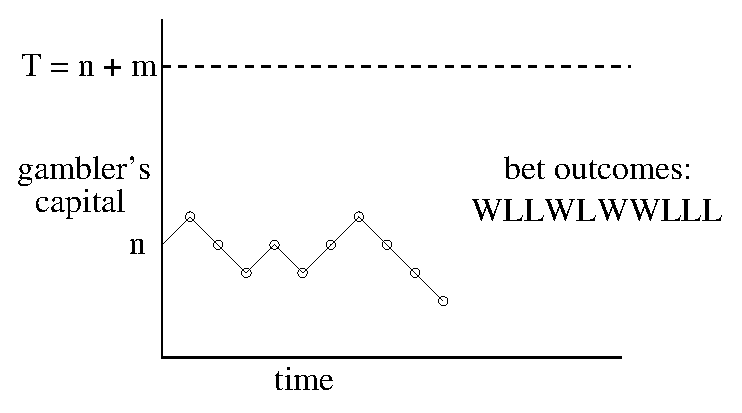
\includegraphics[height=2.5in]{figures/walk1}}
  \caption{\em This is a graph of the gambler's capital versus time
  for one possible sequence of bet outcomes.  At each time step, the
  graph goes up with probability $p$ and down with probability $1-p$.
  The gambler continues betting until the graph reaches either 0 or $T
  = n + m$.}
  \label{LN12:fig:walk1}
\end{figure}

In a \emph{fair} game, the gambler is equally likely to win or lose each
bet, that is $p = 1/2$.  The corresponding random walk is called {\em
  unbiased}.  The gambler is more likely to win if $p>1/2$ and less likely
to win if $p<1/2$; the corresponding random walks are called {\em biased}.
We want to determine the probability that the walk terminates at boundary
$T$, namely, the probability that the gambler is a winner.  We'll do this
by showing that the probability satisfies a simple linear recurrence and
solving the recurrence, but before we derive the probability, let's just
look at what it turns out to be.

\iffalse

\subsection{The Probability Space}

Each random-walk game corresponds to a path like the one in
Figure~\ref{LN12:fig:walk1} that starts at the point $(n,0)$.  A winning path
never touches the $x$ axis and ends when it first touches the line $y=T$.
Likewise, a losing path never touches the line $y=T$ and ends when it first
touches the $x$ axis.

\setlength{\unitlength}{0.0125in}
%
\begingroup\makeatletter\ifx\SetFigFont\undefined
% extract first six characters in \fmtname
\def\x#1#2#3#4#5#6#7\relax{\def\x{#1#2#3#4#5#6}}%
\expandafter\x\fmtname xxxxxx\relax \def\y{splain}%
\ifx\x\y   % LaTeX or SliTeX?
\gdef\SetFigFont#1#2#3{%
  \ifnum #1<17\tiny\else \ifnum #1<20\small\else
  \ifnum #1<24\normalsize\else \ifnum #1<29\large\else
  \ifnum #1<34\Large\else \ifnum #1<41\LARGE\else
     \huge\fi\fi\fi\fi\fi\fi
  \csname #3\endcsname}%
\else
\gdef\SetFigFont#1#2#3{\begingroup
  \count@#1\relax \ifnum 25<\count@\count@25\fi
  \def\x{\endgroup\@setsize\SetFigFont{#2pt}}%
  \expandafter\x
    \csname \romannumeral\the\count@ pt\expandafter\endcsname
    \csname @\romannumeral\the\count@ pt\endcsname
  \csname #3\endcsname}%
\fi
\fi\endgroup
\begin{picture}(300,175)(0,-10)
\path(40,160)(40,0)
\path(20,40)(300,40)
\dottedline{5}(20,140)(300,140)
\path(40,80)(60,100)(80,80)
	(100,100)(120,120)(140,100)
	(160,120)(180,100)(200,80)
	(220,60)(240,80)(260,100)
	(280,120)(300,140)
\put(0,140){\makebox(0,0)[lb]{\smash{{{\SetFigFont{12}{14.4}{rm}T}}}}}
\put(0,40){\makebox(0,0)[lb]{\smash{{{\SetFigFont{12}{14.4}{rm}0}}}}}
\put(60,20){\makebox(0,0)[lb]{\smash{{{\SetFigFont{12}{14.4}{rm}1}}}}}
\put(80,20){\makebox(0,0)[lb]{\smash{{{\SetFigFont{12}{14.4}{rm}2}}}}}
\put(100,20){\makebox(0,0)[lb]{\smash{{{\SetFigFont{12}{14.4}{rm}3}}}}}
\put(0,80){\makebox(0,0)[lb]{\smash{{{\SetFigFont{12}{14.4}{rm}n}}}}}
\end{picture}

Any length $k$ path can be characterized by the history of wins and losses
on individual \$1 bets, so we use a length $k$ string of $W$'s and $L$'s to
model a path, and assign probability $p^rq^{k-r}$ to a string that contains
$r$ $W$'s.  The \emph{outcomes} in our sample space will be precisely those
string corresponding to winning or losing walks.

What about the infinite walks in which the gambler plays forever, neither
reaching his target nor going bankrupt?  A recitation problem will show the
probability of playing forever is zero, so we don't need to include any
such outcomes in our sample space.

As a sanity check on this definition of the probability space, we should
verify that the sum of the outcome probabilities is one, but we omit this
calculation.

To do this, we
let $X$ be any string of $W$'s and $L$'s, and let $[X]$ be the event
consisting of the outcomes that begin with $X$.  If $X$ itself is not an
outcome but begins with an outcome, then $[X] = \emptyset$ so $\pr{[X]} =
0$.  On the other hand, if no prefix of $X$ is an outcome, then it's easy
to verify by induction on $k$ that $\pr{[X]} = p^rq^{k-r}$.  length $k$

%%%COMPLETE

We'll leave this to the reader.
\fi

%\subsection{The Probability of Winning}

%\subsubsection{The Unbiased Game}

Let's begin by supposing the coin is fair, the gambler starts with $100$
dollars, and he wants to double his money.  That is, he plays until he
goes broke or reaches a target of $200$ dollars.  Since he starts
equidistant from his target and bankruptcy, it's clear by symmetry that
his probability of winning in this case is 1/2.

We'll show below that starting with $n$ dollars and aiming for a target of
$T \geq n$ dollars, the probability the gambler reaches his target before
going broke is $n/T$.  For example, suppose he want to win the same \$100,
but instead starts out with \$500.  Now his chances are pretty good: the
probability of his making the 100 dollars is $5/6$.  And if he started
with one million dollars still aiming to win \$100 dollars he almost
certain to win: the probability is $1M/(1M + 100) > .9999$.

So in the fair game, the larger the initial stake relative to the target,
the higher the probability the gambler will win, which makes some
intuitive sense.  But note that although the gambler now wins nearly all
the time, the game is still fair.  When he wins, he only wins \$100; when
he loses, he loses big: \$1M.  So the gambler's average win is actually
zero dollars.

\iffalse
\begin{example}
Suppose Albert starts with \$100, and Eric starts with \$10.  They flip a
fair coin, and every time a Head appears, Albert wins \$1 from Eric, and
vice versa for Tails.  They play this game until one person goes bankrupt.
What is the probability of Albert winning?

This problem is identical to the Gambler's Ruin problem with $n=100$ and
$T=100+10=110$.  The probability of Albert winning is $100/110 = 10/11$,
namely, the ratio of his wealth to the combined wealth.  Eric's chances of
winnning are $1/11$.
\fi

%\subsubsection{The Biased Game}

Now suppose instead that the gambler chooses to play roulette in an
American casino, always betting \$1 on red.  A roulette wheel has 18 black
numbers, 18 red numbers, and 2 green numbers, designed so that each number
is equally likely to appear.  So this game is slightly biased against the
gambler: the probability of winning a single bet is $p = 18/38 \approx
0.47$.  It's the two green numbers that slightly bias the bets and give
the casino an edge.  Still, the bets are almost fair, and you might expect
that starting with \$500, the gambler has a reasonable chance of winning
\$100 ---the 5/6 probability of winning in the unbiased game surely gets
reduced, but perhaps not too drastically.

Not so!  The gambler's odds of winning \$100 making one dollar bets
against the ``slightly'' unfair roulette wheel are less than 1 in 37,000.
If that seems surprising, listen to this: \emph{no matter how much money}
the gambler has to start ---\$5000, \$50,000, $\$5 \cdot 10^{12}$ ---his
odds are still less than 1 in 37,000 of winning a mere 100 dollars!

Moral:  Don't play!

The theory of random walks is filled with such fascinating and
counter-intuitive conclusions.

\subsection{A Recurrence for the Probability of Winning}

The probability the gambler wins is a function of his initial capital,
$n$, his target, $T \geq n$, and the probability, $p$, that he wins an
individual one dollar bet.  Let's let $p$ and $T$ be fixed, and let $w_n$
be the gambler's probabiliity of winning when his initial capital is $n$
dollars.  For example, $w_0$ is the probability that the gambler will win
given that he starts off broke and $w_T$ is the probability he will win if
he starts off with his target amount, so clearly
\begin{align}
w_0 & = 0,\label{LN12:w0}\\
w_T & = 1. \label{LN12:wT}
\end{align}

Otherwise, the gambler starts with $n$ dollars, where $0 < n < T$.
Consider the outcome of his first bet.  The gambler wins the first bet
with probability $p$.  In this case, he is left with $n+1$ dollars and
becomes a winner with probability $w_{n+1}$.  On the other hand, he loses
the first bet with probability $q \eqdef 1-p$.  Now he is left with $n-1$
dollars and becomes a winner with probability $w_{n-1}$.  By the Total
Probability Rule, he wins with probability $w_n = p w_{n+1} + q w_{n-1}$.
Solving for $w_{n+1}$ we have
\begin{equation}\label{LN12:rec1}
w_{n+1} = \frac{w_n}{p} -r w_{n-1}
\end{equation}
where
\[
r \eqdef \frac{q}{p}.
\]

This recurrence holds only for $n+1 \leq T$, but there's no harm in
using~\eqref{LN12:rec1} to define $w_{n+1}$ for all $n+1 >1$.  Now, letting
\[
W(x) \eqdef w_0 + w_1x + w_2x^2 + \cdots
\]
be the generating function for the $w_n$, we derive from~\eqref{LN12:rec1}
and~\eqref{LN12:w0} using our generating function methods that
\iffalse
\[
\frac{xW(x)}{p} - \frac{q}{p}x^2W(x) = W(x) - w_1x,
\]
so
\fi
\begin{equation}\label{LN12:Wx}
W(x) = \frac{w_1x}{(1-x)(1-rx)},
\end{equation}
%= \frac{w_1x}{(q/p)x^2-(x/p)+1}

so if $p \neq q$, then using partial fractions we can calculate that
\iffalse
\begin{equation}\label{LN12:WAB}
W(x)= \frac{A}{1-x} + \frac{B}{1-(q/p)x}.
\end{equation}
where $A=w_1/(1-(q/p))$

From~\eqref{LN12:Wx} and~\eqref{LN12:WAB}, we have
\[
w_1x = A(1-(q/p)x) + B(1-x).
\]
Letting $x=1$, we get $A=w_1/(1-(q/p))$, and letting $x=p/q$, we get
$B=-w_1/(1-(q/p))$, so
\fi

\[
W(x) = \frac{w_1}{r-1} \paren{\frac{1}{1-rx} - \frac{1}{1-x}},
\]
which implies
\begin{equation}\label{LN12:withw1}
w_n = w_1\frac{r^n - 1}{r-1}.
\end{equation}

Now we can use~\eqref{LN12:withw1} to solve for $w_1$ by letting $n=T$ to get
\iffalse
\[
1=w_T = \frac{w_1}{(q/p)-1}\paren{\paren{\frac{q}{p}}^T - 1}
\]
so
\fi
\[
w_1= \frac{r - 1}{r^T-1}.
\]
Plugging this value of $w_1$ into~\eqref{LN12:withw1}, we finally arrive at
the solution:
\begin{equation}\label{LN12:wnsol}
w_n = \frac{r^n-1}{r^T -1}. 
\end{equation}

\iffalse
Our derivation of~(\ref{LN12:wnsol}) ensures that it gives a formula for $w_n$
which satisfies~(\ref{LN12:rec1}) and has the right values at $n=0$ and $n=T$.
Moreover, the values determined by~(\ref{LN12:wnsol}) are the \emph{only ones}
that satisfy~(\ref{LN12:rec1}) and the boundary conditions at $0$ and $T$,
though we won't prove this.  This implies that the Gambler's probability
of winning is indeed given by~(\ref{LN12:wnsol}).
\fi

The expression~\eqref{LN12:wnsol} for the probability that the Gambler wins
in the biased game is a little hard to interpret.  There is a simpler
upper bound which is nearly tight when the gambler's starting capital is
large and the game is biased {\em against} the
gambler.  Then both the numerator and denominator in the quotient
in~\eqref{LN12:wnsol} are positive, and the quotient is less than one.  This
implies that
\[
w_n < \frac{r^n}{r^T} = r^{T-n}, 
\]
which proves:
\begin{corollary}\label{LN12:biaswincor}
  In the Gambler's Ruin game with probability $p< 1/2$ of winning each
  individual bet, with initial capital, $n$, and target, $T$,
\begin{equation}\label{LN12:biaswinsimp}
\pr{\text{the gambler is a winner}} < \paren{\frac{p}{q}}^{T-n}
\end{equation}
\end{corollary}

The amount $T-n$ is called the Gambler's \emph{intended profit}.  So the
gambler gains his intended profit before going broke with probability at
most $p/q$ raised to the intended-profit power.  Notice that this upper
bound does not depend on the gambler's starting capital, but only on his
intended profit.  This has the amazing consequence we announced above:
\emph{no matter how much money he starts with}, if he
makes \$1 bets on red in roulette aiming to win \$100, the
probability that he wins is less than
\[
\paren{\frac{18/38}{20/38}}^{100} = \paren{\frac{9}{10}}^{100} < \frac{1}{37,648}.
\]

The bound~(\ref{LN12:biaswinsimp}) is exponential in the intended profit.  So,
for example, doubling his intended profit will square his probability of
winning.  In particular, the probability that the gambler's stake goes up
$200$ dollars before he goes broke playing roulette is at most
\[
(9/10)^{200} = ((9/10)^{100})^2 = \left(\frac{1}{37,648}\right)^2,
\]
which is about 1 in 70 billion.

\iffalse

The odds of winning a little money are not so bad.
Applying the exact formula~\eqref{LN12:wnsol}, we find that the probability
of winning \$10 before losing \$10 is
\[
\frac{\paren{\frac{20/38}{18/38}}^{10} - 1}
              {\paren{\frac{20/38}{18/38}}^{20} - 1}
  = 0.2585\dots.
\]
This is somewhat worse than the 1 in 2 chance in the fair game, but not
dramatically so.
\fi

The solution~(\ref{LN12:wnsol}) only applies to biased walks, but the method
above works just as well in getting a formula for the unbiased case
(except that the partial fractions involve a repeated root).  But it's
simpler settle the fair case simply by taking the limit as $r$
approaches 1 of~\eqref{LN12:wnsol}.  By L'Hopital's Rule this limit is $n/T$,
as we claimed above.

\subsection{Intuition}

Why is the gambler so unlikely to make money when the game is slightly
biased against him?  Intuitively, there are two forces at work.  First,
the gambler's capital has random upward and downward {\em swings} due to
runs of good and bad luck.  Second, the gambler's capital will have a
steady, downward {\em drift}, because the negative bias means an average
loss of a few cents on each \$1 bet.  The situation is shown in
Figure~\ref{LN12:fig:walk2}.

\iffalse
For example, in roulette the gambler wins a dollar with probability $9/19$
and loses a dollar with probability $10/19$.  Therefore, his average
return on each bet is $9/10 - 10/19 = - 1/19 \approx -0.053$ dollars.
That is, on each bet his capital is can be expected to drift downward by a
little over 5 cents.
\fi

Our intuition is that if the gambler starts with, say, a billion dollars,
then he is sure to play for a very long time, so at some point there
should be a lucky, upward swing that puts him \$100 ahead.  The problem is
that his capital is steadily drifting downward.  If the gambler does not
have a lucky, upward swing early on, then he is doomed.  After his capital
drifts downward a few hundred dollars, he needs a huge upward swing to
save himself.  And such a huge swing is extremely improbable.  As a rule
of thumb, \emph{drift dominates swings} in the long term.

%\begin{nooutline}
\begin{figure}
\centerline{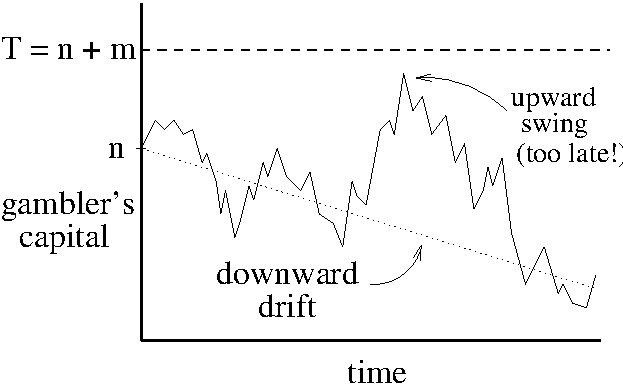
\includegraphics[height=2.5in]{figures/walk2}}
\caption{\em In an unfair game, the gambler's capital swings randomly up
and down, but steadily drifts downward.  If the gambler does not have
a winning swing early on, then his capital drifts downward, and later
upward swings are insufficient to make him a winner.}
\label{LN12:fig:walk2}
\end{figure}
%\end{nooutline}

\iffalse

We can quantify these drifts and swings.  After $k$ rounds for $k \le
\min(m,n)$, the number of wins by our player has a binomial distribution
with parameters $p < 1/2$ and $k$.  His expected win on any single bet is
$p-q = 2p-1$ dollars, so his expected capital is $n-k(1-2p)$.  Now to be a
winner, his actual number of wins must exceed the expected number by
$m+k(1-2p)$.  But we saw before that the binomial distribution has a
standard deviation of only $\sqrt{kp(1-p)}$.  So for the gambler to win,
he needs his number of wins to deviate by
\[
\frac{m+k(1-2p)}{\sqrt{kp(1-2p)}}=\Theta(\sqrt{k})
\]
times its standard deviation.  In our study of binomial tails we saw that
this was extremely unlikely.

In a fair game, there is no drift; swings are the only effect.  In the
absence of downward drift, our earlier intuition is correct.  If the
gambler starts with a trillion dollars then almost certainly there
will eventually be a lucky swing that puts him \$100 ahead.

If we start with \$10 and play to win only \$10 more, then the difference
between the fair and unfair games is relatively small. We saw that the
probability of winning is $1/2$ versus about $1/4$.  Since swings of \$10
are relatively common, the game usually ends before the gambler's capital
can drift very far.  That is, the game does not last long enough for drift
to dominate the swings.

\subsection{How Long a Walk?}

Now that we know the probability, $w_n$, that the gambler is a winner in
both fair and unfair games, we consider how many bets he needs on average
to either win or go broke.

\subsection{Duration of a Biased Walk}

Let $Q$ be the number of bets the gambler makes until the game ends.  Since
the gambler's expected win on any bet is $2p-1$, Wald's Theorem should tell
us that his game winnings, $G$, will have expectation $\expect{Q}(2p-1)$.
That is,
\begin{equation}\label{LN12:gw}
\expect{G} = (2p-1)\expect{Q},
\end{equation}

In an unbiased game~(\ref{LN12:gw}) is trivially true because both $2p-1$ and
the expected overall winnings, $\expect{G}$, are zero.  On the other hand,
in the unfair case, $2p-1 \neq 0$.  Also, we know that
\[
\expect{G} = w_n(T-n) - (1-w_n)n = w_nT-n.
\]
So assuming~(\ref{LN12:gw}), we conclude
\begin{theorem}\label{LN12:ExQthm}
In the biased Gambler's Ruin game with initial capital, $n$, target,
$T$, and probability, $p \neq 1/2$, of winning each bet,
\begin{equation}\label{LN12:ExQ}
\expect{\text{number of bets till game ends}} =
\frac{\pr{\text{gambler is a winner}}T-n}{2p-1}.
\end{equation}
\end{theorem}

The only problem is that~(\ref{LN12:gw}) is not a special case of Wald's
Theorem because $G = \sum_{i=1}^Q G_i$ is not a sum of \emph{nonnegative}
variables: when the gambler loses the $i$th bet, the random variable $G_i$
equals $-1$.  However, this is easily dealt with.\footnote{The random variable
$G_i+1$ is nonnegative, and $\expcond{G_i+1}{Q \geq i} =
\expcond{G_i}{Q\geq i}+1 = 2p$, so by Wald's Theorem
\begin{equation}\label{LN12:G1}
\expect{\sum_{i=1}^Q (G_i+1)}  = 2p\expect{Q}.
\end{equation}
But
\begin{eqnarray}
\expect{\sum_{i=1}^Q (G_i+1)} & = & \expect{\sum_{i=1}^Q G_i + \sum_{i=1}^Q 1}\notag\\
   & = & \expect{(\sum_{i=1}^Q G_i) + Q}\notag\\
   & = & \expect{\sum_{i=1}^Q G_i} + \expect{Q}\notag\\
   & = & \expect{G} + \expect{Q}\label{LN12:GQ}.
\end{eqnarray}
Now combining~(\ref{LN12:G1}) and~(\ref{LN12:GQ}) confirms the truth of our
assumption~(\ref{LN12:gw}).}

\begin{example}
If the gambler aims to profit \$100 playing roulette with $n$ dollars to
start, he can expect to make $((n+100)/37,648 - n)/(2(18/38) - 1) \approx
19n$ bets before the game ends.  So he can enjoy playing for a good while
before almost surely going broke.
\end{example}


\subsection{Duration of an Unbiased Walk}

This time, we need the more general approach of recurrences to handle the
unbiased case.  We consider the expected number of bets as a
function of the gambler's initial capital.  That is, for fixed $p$ and $T$,
let $e_n$ be the expected number of bets until the game ends when the
gambler's initial capital is $n$ dollars.  Since the game is over in no
steps if $n=0$ or $T$, the boundary conditions this time are $e_0=e_T=0$.

Otherwise, the gambler starts with $n$ dollars, where $0 < n < T$.
Now by the conditional expectation rule, the expected number of steps can
be broken down into the expected number of steps given the outcome of the
first bet weighted by the probability of that outcome.  That is,
\[
e_n = p\expcond{Q}{\text{gambler wins first bet}} +
q\expcond{Q}{\text{gambler loses first bet}}.
\]
But after the gambler wins the first bet, his capital is $n+1$, so
he can expect to make another $e_{n+1}$ bets.  That is,
\[
\expcond{Q}{\text{gambler wins first bet}} = 1 + e_{n+1},
\]
and similarly, 
\[
\expcond{Q}{\text{gambler loses first bet}} = 1 + e_{n-1}.
\]
So we have
\[
e_n =  p(1 + e_{n+1}) +  q(1 + e_{n-1}) =  pe_{n+1} + qe_{n-1} + 1, 
\]
which yields the linear recurrence
\[
e_{n+1} = \frac{e_n}{p} - \frac{q}{p} e_{n-1} - \frac{1}{p}.
\]
For $p = q = 1/2$, this equation simplifies to
\begin{equation}\label{LN12:en2}
e_{n+1} = 2e_n - e_{n-1} - 2.
\end{equation}
There is a general theory for solving linear recurrences like~(\ref{LN12:en2})
in which the value at $n+1$ is a linear combination of values at some
arguments $k<n+1$ plus another simple term---in this case plus the constant
$-2$.  This theory implies that
\begin{equation}\label{LN12:Tn}
e_n  = (T - n)n.
\end{equation}
Fortunately, we don't need the general theory to \emph{verify} this
solution.  Equation~(\ref{LN12:Tn}) can be verified routinely from the boundary
conditions and~(\ref{LN12:en2}) using strong induction on $n$.

So we have shown
\begin{theorem}\label{LN12:fairtime}
In the unbiased Gambler's Ruin game with initial capital, $n$, and target,
$T$, and probability, $p = 1/2$, of winning each bet,
\begin{equation}
\expect{\text{number of bets till game ends}} = n(T-n).
\end{equation}
\end{theorem}

Another way to phrase Theorem~\ref{LN12:fairtime} is
\begin{equation}\label{LN12:mn}
\expect{\text{number of bets till game ends}} = \text{initial capital}
\cdot \text{intended profit}.
\end{equation}

Now for example, we can conclude that if the gambler starts with \$10
dollars and plays until he is broke or ahead \$10, then $10 \cdot 10 = 100$
bets are required on average.  If he starts with \$500 and plays until he
is broke or ahead \$100, then the expected number of bets until the game is
over is $500 \times 100 = 50,000$.

Notice that~(\ref{LN12:mn}) is a very simple answer that cries out for an
intuitive proof, but we have not found one.
\fi

\iffalse

\textbf{Below is my try at the suggestion of Santosh and Adam Kalai for an
example requiring a Pairwise \Emph{Uncorrlelated} Sampling Theorem.  But I
don''t think this goes anywhere. }

\subsection{Fluctuations in an Unbiased Walk}

Let's consider the probability that the game ends within $k$ flips.  This
number is awkward to calculate explicitly, but we will be able to estimate
it using our methods for estimating expected deviation from the mean.

Let $C_k$ be the gamblers capital after $k$ flips.  That is,
\[
C_k \eqdef n + \sum_{i=1}^k G_i.
\]
In the unbiased case, the expected win on one flip is zero, so since $C_k$
is the sum of variables which have expectation 0, it follows that
$\expect{C_k} = 0$.  What about $\variance{C_k}$?  We will prove that
\begin{equation}\label{LN12:sumvarg}
\variance{C_k} = \sum_{i=1}^k \variance{G_i}.
\end{equation}

Note that for $i \neq j$, $G_i$ and $G_j$ are not independent, and so we
cannot appeal to pairwise independent additivity of variance to
prove~(\ref{LN12:sumvarg}).  For example, if $G_i = 0$, then the game has
stopped before the $i$th flip, so if $j > i$, then $G_j = 0$.  On the
other hand, the probability that $G_j = 0$ is less than one, because there
is some positive probability that the game will continue for more than $j$
flips (except for the degenerate case when $n=1 and T=2$).  That is,
\[
\prcond{G_j = 0}{G_i = 0} = 1 > \pr{G_j = 0},
\]
confirming nonindependence.

However, inspection of the proof of pairwise independent additivity of
variance shows that it didn't really require pairwise independence!  The
only property of the variables being added is that they be pairwise
\emph{uncorrelated}:

\begin{definition*}
Random variables $R$ and $S$ are \emph{uncorrelated} iff
\begin{equation}\label{LN12:uncor}
\expect{RS} = \expect{R}\expect{S}.
\end{equation}
\end{definition*}

\begin{lemma}\label{LN12:Guncor}
For $i \neq j$, $G_i$ and $G_j$ are uncorrelated.
\end{lemma}
\fi

\iffalse
\subsection{Quit While You Are Ahead}

Suppose that the gambler never quits while he is ahead.  That is, he
starts with $n>0$ dollars, ignores any target $T$, but plays until he is
flat broke.  Then it turns out that if the game is not favorable, \ie $p
\leq 1/2$, the gambler is sure to go broke.  In particular, he is even
sure to go broke in a ``fair'' game with $p = 1/2$.
\footnote{If the game is favorable to the gambler, \ie $p>1/2$, then we
could show that there is a positive probability that the gambler will play
forever, but we won't examine this case in these Notes.}
\begin{lemma}\label{LN12:go broke}
If the gambler starts with one or more dollars and plays a fair game until
he is broke, then he will go broke with probability 1.
\end{lemma}

\begin{proof}
If the gambler has initial capital $n$ and goes broke in a game without
reaching a target $T$, then he would also go broke if he were playing and
ignored the target.  So the probability that he will lose if he keeps
playing without stopping at any target $T$ must be at least as large as the
probability that he loses when he has a target $T>n$.

But we know that in a fair game, the probability that he loses is $1 -
n/T$.  This number can be made arbitrarily close to 1 by choosing a
sufficiently large value of $T$.  Hence, the probability of his losing
while playing without any target has a lower bound arbitrarily close to 1,
which means it must in fact be 1.
\end{proof}

So even if the gambler starts with a million dollars and plays a perfectly
fair game, he will eventually lose it all with probability 1.  In fact, if
the game is unfavorable, then Theorem~\ref{LN12:ExQthm} and
Corollary~\ref{LN12:biaswincor} imply that his expected time to go broke is
essentially proportional to his initial capital, \ie $\Theta(n)$.

But there is good news: if the game is fair, he can ``expect'' to play for
a very long time before going broke; in fact, he can expect to play
forever!

\begin{lemma}\label{LN12:play forever}
If the gambler starts with one or more dollars and plays a fair game until
he goes broke, then his expected number of plays is infinite.
\end{lemma}

\begin{proof}
Consider the gambler's ruin game where the gambler starts with initial
capital $n$, and let $u_n$ be the expected number of bets for
the \emph{unbounded} game to end.  Also, choose any $T \geq n$, and as
above, let $e_n$ be the expected number of bets for the game to end when
the gambler's target is $T$.

The unbounded game will have a larger expected number of bets compared to
the bounded game because, in addition to the possibility that the gambler
goes broke, in the bounded game there is also the possibility that the
game will end when the gambler reaches his target, $T$.  That is,
\[
u_n \geq e_n.
\]
So by~(\ref{LN12:Tn}), 
\[
u_n \geq n(T-n).
\]
But $n \geq 1$, and $T$ can be any number greater than or equal to $n$, so
this lower bound on $u_n$ can be arbitrarily large.  This implies that
$u_n$ must be infinite.

Now by Lemma~\ref{LN12:go broke}, with probability 1, the unbounded game ends
when the gambler goes broke.  So the expected time for the unbounded game
to \emph{end} is the \emph{same} as the expected time for the gambler to
\emph{go broke}.  Therefore, the expected time to go broke is infinite.
\end{proof}

In particular, even if the gambler starts with just one dollar, his
expected number of plays before going broke is infinite!  Of course, this
does not mean that it is likely he will play for long.  For example, there
is a 50\% chance he will lose the very first bet and go broke right away.

Lemma~\ref{LN12:play forever} says that the gambler can ``expect'' to play
forever, while Lemma~\ref{LN12:go broke} says that with probability 1 he will
go broke.  These Lemmas sound contradictory, but our analysis showed that
they are not.  A moral is that naive intuition about ``expectation'' is
misleading when we consider limiting behavior according to the technical
mathematical definition of expectation.
\fi

%% Gamblers' Ruin Problems %%%%%%%%%%%%%%%%%%%%%%%%%%%%%%%%%%%%%%%%%%%%%%%%%%%%
%\startclassproblems
%\pinput{CP_}


%% Random Walks on Graphs %%%%%%%%%%%%%%%%%%%%%%%%%%%%%%%%%%%%%%%%%%%%%%%%%%%%%
\section{Random Walks on Graphs}

\hyperdef{page}{rank}{Random walks on graphs arise in all sorts of
  applications.  One interesting example is Google and page rank, which
  we'll explore in this section.}

The hyperlink structure of the World Wide Web can be described as a
digraph. The nodes are the web pages or web-accessible files.  There is a
directed edge from node $x$ to node $y$ if the page associated with $x$
has a link to the page associated with $y$.  For example, in the following
graph the vertices $x_1, \ldots, x_n$ correspond to web pages and
$\diredge{x_i}{x_j}$ is a directed edge when page $x_i$ contains a
hyperlink to page $x_j$.

\mfigure{!}{2in}{figures/randomWalkFigs/webGraph}

The web graph is an enormous graph with many billions and probably even
trillions of nodes. At first glance, this graph wouldn't seem to be very
interesting. But in 1995, two students at Stanford, Larry Page and Sergey
Brin realized that the structure of this graph could be very useful in
building a search engine.  Traditional document searching programs had
been around for a long time and they worked in a fairly straightforward
way.  Basically, you would enter some search terms and the searching
program would return all documents containing those terms.  A relevance
score might also be returned for each document based on the frequency or
position that the search terms appeared in the document.  For example, if
the search term appeared in the title or appeared $100$ times in a
document, that document would get a higher score.  So if an author wanted
a document to get a higher score for certain keywords, he would put the
keywords in the title and make it appear in lots of places.  You can even
see this today with some bogus web sites.

This approach works fine if you only have a few documents that match a
search term.  But on the web, there are billions of documents and millions
of matches to a typical search.

For example, a few years ago a search on Google for ``math for computer
science notes'' gave 378,000 hits!  How does Google decide which 10 or 20
to show first?  It wouldn't be smart to pick a page that gets a high
keyword score because it has ``math math $\dots$ math'' across the front
of the document.

One way to get placed high on the list is to pay Google an advertising
fees ---and Google gets an enormous revenue stream from these fees.  Of
course an early listing is worth a fee only if an advertiser's target
audience is attracted to the listing.  But an audience does get attracted
to Google listings because its ranking method is really good at
determining the most important relevant web pages.  For example, Google
demonstrated its accuracy in our case by giving first rank to the Fall
2002 open courseware page for 6.042 \texttt{:-)} .  So how did Google know
to pick 6.042 to be first out of $378,000$?

Well back in 1995, Larry and Sergey got the idea to allow the digraph
structure of the web to determine which pages are likely to be the most
important.

\subsection{A First Crack at Page Rank}

Looking at the web graph, any idea which node/page might be the best to
rank $1$st?  Assume that all the pages match the search terms for now.
Well, intuitively, we should choose $x_2$, since lots of other pages point
to it.  This leads us to their first idea: try defining the \emph{page
  rank} of $x$ to be the number of links pointing to $x$, that is,
$\text{indegree}(x)$.  The idea is to think of web pages as voting for the
most important page ---the more votes, the better rank.

Of course, there are some problems with this idea. Suppose you wanted
to have your page get a high ranking.  One thing you could do is to
create lots of dummy pages with links to your page.

\mfigure{!}{1.5in}{figures/randomWalkFigs/dummy}

There is another problem ---a page could become unfairly influential by
having lots of links to other pages it wanted to hype.

\mfigure{!}{1.5in}{figures/randomWalkFigs/outDegree}

So this strategy for high ranking would amount to, ``vote early, vote
often,'' which is no good if you want to build a search engine that's
worth paying fees for.  So, admittedly, their original idea was not so
great.  It was better than nothing, but certainly not worth billions of
dollars.

\subsection{Random Walk on the Web Graph}

But then Sergey and Larry thought some more and came up with a couple of
improvements.  Instead of just counting the indegree of a node, they
considered the probability of being at each page after a long random walk
on the web graph.  In particular, they decided to model a user's web
experience as following each link on a page with uniform probability.
That is, they assigned each edge $x \rightarrow y$ of the web graph with a
probability conditioned on being on page $x$:
\[
\prcond{\text{follow link}\ \diredge{x}{y}}{ \text{at page $x$}} \eqdef
\frac{1}{\text{outdegree}(x)}.
\]
The user experience is then just a random walk on the web graph.

For example, if the user is at page $x$, and there are three links from
page $x$, then each link is followed with probability $1/3$.

We can also compute the probability of arriving at a particular page, $y$,
by summing over all edges pointing to $y$.  We thus have
\begin{eqnarray}
  \pr{\text{go to $y$}} &=&  \sum_{\text{edges}\ \diredge{x}{y}}
  \prcond{\text{follow link}\ \diredge{x}{y}}{\text{at page $x$}} \cdot
  \pr{\text{at page $x$}} \nonumber\\
  &=& \sum_{\text{edges}\ \diredge{x}{y}} \frac{\pr{\text{at
      $x$}}}{\text{outdegree}(x)} \label{LN12:stepprob}
\end{eqnarray}
For example, in our web graph, we have
\[ \pr{\text{go to $x_4$}} = \frac{\pr{\text{at $x_7$}}}{2} +
\frac{\pr{\text{at $x_2$}}}{1} \ .
\]
One can think of this equation as $x_7$ sending half its probability to
$x_2$ and the other half to $x_4$. The page $x_2$ sends all of its
probability to $x_4$.

There's one aspect of the web graph described thus far that doesn't mesh
with the user experience ---some pages have no hyperlinks out.  Under the
current model, the user cannot escape these pages.  In reality, however,
the user doesn't fall off the end of the web into a void of nothingness.
Instead, he restarts his web journey.

To model this aspect of the web, Sergey and Larry added a supernode to the
web graph and had every page with no hyperlinks point to it.  Moreover,
the supernode points to every other node in the graph, allowing you to
restart the walk from a random place.  For example, below left is a graph
and below right is the same graph after adding the supernode $x_{N+1}$.

\bigskip\centerline{
  \resizebox{!}{1.3in}{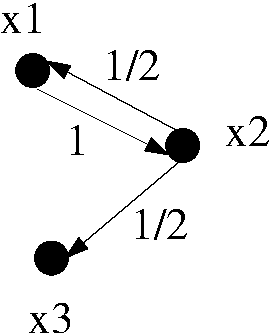
\includegraphics{figures/randomWalkFigs/adjMatrix2}}
  \hspace{2cm}
  \resizebox{!}{1.5in}{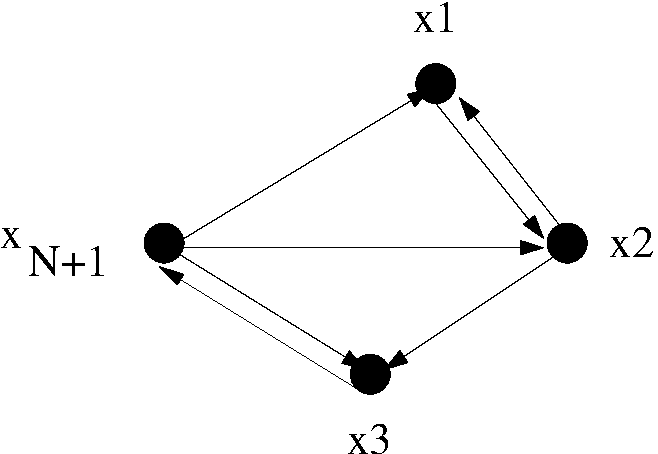
\includegraphics{figures/randomWalkFigs/sinkGraph}}
}\bigskip

The addition of the supernode also removes the possibility that the value
$1/\text{outdegree}(x)$ might involve a division by zero.

\subsection{Stationary Distribution \& Page Rank}

Page rank is basically just a stationary distribution over the web
graph (there are some more details, but this is the main idea), so
let's define a stationary distribution.

Suppose each node is assigned a probability that corresponds, intuitively,
to the likelihood that a random walker is at that node at a randomly
chosen time.  We assume that the walk never leaves the nodes in the graph,
so we require that
\begin{equation}\label{LN12:sum1}
\sum_{\text{nodes}\ x} \pr{\text{at $x$}} = 1.
\end{equation}

\begin{definition} An assignment of probabililties to nodes in a digraph
  is a \term{stationary distribution} if for all nodes $x$
\[
\pr{\text{at $x$}} = \pr{\text{go to $x$ at next step}}
\]
\end{definition}  

Sergey and Larry defined their page ranks to be a stationary distribution
They did this by solving the following system of linear equations: find a
nonnegative number, $\text{PR}(x)$, for each node, $x$, such that
\begin{equation}\label{LN12:PReqs}
\text{PR}(x) = \sum_{\text{edges}\ \diredge{y}{x}} \frac{\text{PR}(y)}{\text{outdegree}(y)},
\end{equation}
corresponding to the intuitive equations given in \eqref{LN12:stepprob}.  These
numbers must also satisfy the additional constraint corresponding
to~\eqref{LN12:sum1}:
\begin{equation}\label{LN12:sum1PR}
\sum_{\text{nodes}\ x} \text{PR}(x) = 1.
\end{equation}
So if there are $n$ nodes, then equations~\eqref{LN12:PReqs} and~\eqref{LN12:sum1PR}
provide a system of $n+1$ linear equations in the $n$ variables,
$\text{PR}(x)$.  Note that constraint~\eqref{LN12:sum1PR} is needed because the
remaining constraints~\eqref{LN12:PReqs} could be satisfied by letting
$\text{PR}(x)\eqdef 0$ for all $x$, which is useless.

Sergey and Larry were smart fellows, and they set up their page rank
algorithm so it would always have a meaningful solution.  Their addition
of a supernode ensures there is always a \emph{unique} stationary
distribution.  Moreover, starting from \emph{any} node and taking a
sufficiently long random walk on the graph, the probability of being at
each page will get closer and closer to the stationary distribution.  Note
that general digraphs without supernodes may have neither of these
properties: there may not be a unique stationary distribution, and even
when there is, there may be starting points from which the probabilities
of positions during a random walk do not converge to the stationary
distribution.  

\iffalse

\begin{optional}
Here's a note on solving the system of linear constraints, for the
interested reader.

Let $W$ be the $n \times n$ with the entry $w_{ij}$ (in row $i$ and
column $j$) having the value $w_{ij} = 1/\text{outdegree}(x_i)$ if edge
$x_i \rightarrow x_j$ exists, and $w_{ij} = 0$ otherwise.  For example, in
our last example with the 4-node graph (including the supernode), we have
$W$ given by:
\[
\left( \begin{array}{cccc}
    0 & 1 & 0 & 0 \\
    \frac{1}{2} & 0 & \frac{1}{2} & 0 \\
    0 & 0 & 0 & 1\\
    \frac{1}{3} & \frac{1}{3} & \frac{1}{3} & 0 \end{array} \right)
\]

The system of linear equations can now be described by a single matrix
vector product equation $W^T \vec{P} = \vec{P}$, where $W^T$ denotes the
transpose of $W$, and $\vec{P}$ is the column vector of page probabilities
(ranks):
\[\vec{P}\eqdef
\left( \begin{array}{c}
    \text{PR}(x_1) \\
    \text{PR}(x_2) \\
    \vdots \\
    \text{PR}(x_n) \end{array} \right)
\]
So the $j$th entry of the solultion vector, $\vec{P}$, is
\[
\sum_{1\leq i \leq n} w_{ij} \cdot \text{PR}(x_i) =
\sum_{i \mid x_i \rightarrow x_j} \frac{\text{PR}(x_i)}{\text{outdegree}(x_i)},
\]
which is exactly the constraint corresponding to node $x_j$
in~\eqref{LN12:PReqs}.

If you have taken a linear algebra or numerical analysis course, you
realize that the vector of page ranks is just the \emph{principle
  eigenvector} of the matrix, $W$, of the web graph!  Once you've had such
a course, these values are easy to compute.  Of course, when you are
dealing with matrices of this size, the problem gets a little more
interesting.
\end{optional}
\fi

Now just keeping track of the digraph whose nodes are billions of web
pages is a daunting task.  That's why Google is building power plants.
Indeed, Larry and Sergey named their system Google after the number
$10^{100}$ ---which called a ``googol'' ---to reflect the fact that the
web graph is so enormous.

Anyway, now you can see how 6.042 ranked first out of 378,000 matches.
Lots of other universities used our notes and presumably have links to the
6.042 open courseware site, and the university sites themselves are
legitimate, which ultimately leads to 6.042 getting a high page rank in
the web graph.

%% Random Walks on Graphs Problems %%%%%%%%%%%%%%%%%%%%%%%%%%%%%%%%%%%%%%%%%%%%
%\startclassproblems
%\pinput{CP_}


%% Conclusion %%%%%%%%%%%%%%%%%%%%%%%%%%%%%%%%%%%%%%%%%%%%%%%%%%%%%%%%%%%%%%%%%
\TBA{Conclusion...}

\endinput
 %walks on line & graphs, google rank % *Albert
\fi


\end{document}
